\documentclass[11pt]{report}
\usepackage[version=4]{mhchem}
\usepackage{graphicx}
\usepackage{subfigure}
\usepackage{lscape}
%\usepackage{exscale,relsize}
\usepackage{longtable}
\usepackage{supertabular}
\setlength\LTcapwidth{1\columnwidth}
\setlength\LTleft{0pt}
\setlength\LTright{0.1\columnwidth}
%\usepackage{supertabular}
\usepackage{tabularx}
\usepackage{listings}
\lstset{language=Matlab}
\usepackage{framed}
%\usepackage{mathtools}
\usepackage[numbered,autolinebreaks]{mcode}
\usepackage{booktabs}
\usepackage{multirow}
\usepackage{array}
\usepackage[left=1 in, right=2 in, top = 1 in, bottom=1 in]{geometry}
%\setcounter{secnumdepth}{1}
%\usepackage[colorlinks=false, citebordercolor = 0 0 0, linkbordercolor = 0 0 0, urlbordercolor = 0 0 0 ]{hyperref}
% Font packages
%\usepackage{mathpazo}
%\usepackage{helvet}
%\usepackage{mathptmx}
\usepackage[T1]{fontenc}
\usepackage{nameref}
\usepackage{framed}
\usepackage{fancyvrb}

\newdimen\tw \tw=\textwidth\advance\tw-10pt 

% Defining the look of the titles and section headings
\setcounter{secnumdepth}{3}
\newcommand{\chapterfont}{\Large{\textcolor{stanford}}}

\usepackage{titlesec}
\titleformat{\part}[display]{\color{stanford}\Large\rmfamily}{Part {\thepart}}{0.5em}{}
\titleformat{\chapter}[hang]{\color{stanford}\Large\rmfamily}{{\thechapter}}{0.5em}{\enskip}
%\titleformat{\chapter}[display]{\color{stanford}\large\rmfamily\bfseries}{\chaptertitlename \enskip {\thechapter}}{0.5em}{}
%\titleformat{\chapter}[hang]{\large\rmfamily\bfseries}{{\thesection}}{0.5em}{\enskip}
\titleformat{\section}[hang]{\color{stanford}\large\rmfamily}{{\thesection}}{0.5em}{\enskip}
\titleformat{\subsection}[hang]{\color{stanford}\rmfamily}{{\thesubsection}}{0.5em}{\enskip}
\titleformat{\subsubsection}[hang]{\color{stanford}\itshape\rmfamily}{{\thesubsubsection}}{0.5em}{\enskip}
\titleformat{\paragraph}[runin]{\color{stanford}\itshape\rmfamily}{}{0.5em}{\enskip}


% Use AMS math to get left-flush equations, with math indentention set to be equal to paragraph
% or no indentation
\usepackage[fleqn]{amsmath}
\setlength\mathindent{0.0cm}
%\setlength\mathindent{0.66cm}
\usepackage{exscale,relsize}
% Define the color that we want
\usepackage{xcolor}
\definecolor{light-gray}{gray}{0.95}
\definecolor{shadecolor}{gray}{0.95}
\definecolor{stanford}{RGB}{164,0,29}



% Use Paralist to make bullets in lists flush left
\usepackage{paralist}
\setdefaultleftmargin{1.1cm}{}{}{}{}{}

% Use font packages to change the mathematics font to times new roman.
\usepackage{mathpazo}
%\usepackage{helvet}
%\usepackage{mathptmx}

% Alter the captions to be consistent across all types of tables and figures
% IMPORTANT: Only turn this on for printed final runs, as it causes conflicts
\usepackage[font={color=stanford,rm,footnotesize},labelsep=colon,justification=justified,singlelinecheck=false]{caption}
\captionsetup[table]{position=below}
\captionsetup[figure]{position=above}

% Control the placement of captions above and below tables and figures
%\usepackage{floatrow}
%\floatsetup[table]{style=plaintop,justification=justified}
%\floatsetup[figure]{justification=justified}

% Allow better bibliography styles
\usepackage[sort&compress,numbers]{natbib}
%\usepackage{cite}
\usepackage{url}
\usepackage{hyperref}
\usepackage{fancyvrb}

\hyphenation{estimator}
\hyphenation{injection}

% Declaring definitions that are used throughout the ROMEO documentation
%\DeclareMathAlphabet{\mathsf}{T1}{cmss}{m}{n}
\newcommand{\prm}[1]{\textsf{#1}}
%\newcommand{\prm}[1]{\texttt{#1}}
\newcommand{\mprm}[1]{\mathrm{#1}}
%\newcommand{\mprm}[1]{\mathtt{#1}}
\newcommand{\file}[1]{\textrm{#1}}
\newcommand{\arbtitle}[1]{\textrm{\Large{#1}}}
\newcommand{\marg}[1]{{\footnotesize\textit{\textcolor{stanford}{'#1'}}}}
\newcommand{\xlname}[1]{\raisebox{1pt}{\fcolorbox{light-gray}{light-gray}{\texttt{\textcolor{stanford}{\footnotesize{#1}}}}}}
\newcommand{\cellref}[1]{\raisebox{1pt}{\fcolorbox{stanford}{light-gray}{\texttt{\textcolor{stanford}{\scriptsize{#1}}}}}}


%
%\def\UrlFont{}
\newcommand{\boxtitle}[1]{\textcolor{stanford}{#1}}
\newcommand{\marginnote}[1]{\marginpar{\marg{#1}}}
\newcommand{\margcellref}[1]{\marginpar{\cellref{#1}}}
\newcommand{\margcellrefsheet}[2]{\marginpar{\marg{#1}}\marginpar{\cellref{#2}}}

\newcommand{\version}{v3.0a}
\newcommand{\sheet}[1]{\textit{`{#1}'}}
\newcommand{\stream}[1]{\begin{footnotesize}{\textcolor{stanford}{$\overrightarrow{#1}$}}\end{footnotesize}}
\newcommand{\mstream}[1]{{\scriptscriptstyle{\textcolor{stanford}{\overrightarrow{#1}\!}}}}

\newcommand{\eqnunit}[1]{\quad\quad \scriptstyle{\left[\text{#1}\right]}}
\newcommand{\eqnunitfrac}[2]{\quad\quad \scriptstyle{\left[\frac{\text{#1}}{\text{#2}}\right]}}


\setcounter{tocdepth}{1}

%% Define a new 'leo' style for the package that will use a smaller font.
\makeatletter
\def\url@leostyle{%
\@ifundefined{selectfont}{\def\UrlFont{\sf}}{\def\UrlFont{\small\ttfamily}}}
\makeatother
%% Now actually use the newly defined style.
\urlstyle{leo}

%\hypersetup{
% pdfauthor = {},
% pdftitle = {},
% pdfsubject = {},
% pdfkeywords = {},
% pdfcreator = {LaTeX with hyperref package}
%}

\usepackage{fancyhdr}
\pagestyle{fancyplain}
\fancyhf{}
\lhead{\fancyplain{}{\footnotesize{\textrm{El-Houjeiri and Brandt}}}}
\chead{\fancyplain{}{\footnotesize{\textrm{OPGEE \version \; Documentation}}}}
\rhead{\fancyplain{}{\footnotesize{\textrm{\thepage}}}}

% Defining the spacing for the run-in heading on paragraphs.
\titlespacing{\paragraph}{-0.38cm}{0.5em}{0.5em}[0cm]

%Changing the look of the description environment
\renewcommand\descriptionlabel[1]{\hspace{\labelsep}\textbf{#1}}

\usepackage[ugly]{units}
\usepackage{amssymb}
\usepackage{marvosym}
\usepackage{longtable}
\usepackage{threeparttable}



\begin{document}

\thispagestyle{plain}
\noindent \arbtitle{\\
\\
\linethickness{0.6mm} \line(1,0){450}\\
\\
{{\textcolor{stanford}{Oil Production Greenhouse Gas Emissions Estimator \\
\\
OPGEE \version \;\\ 
\\
\large{User guide \& Technical documentation} }}}}
\\
\linethickness{0.6mm} \line(1,0){450}\\
\\
\\
\noindent 
\textrm{\\
\\
Hassan M. El-Houjeiri,$^{1,\star}$ Mohammad S. Masnadi,$^1$ Kourosh Vafi,$^{1,\star}$ Patrick Perrier,$^{1}$ James Duffy,$^2$ Adam R. Brandt$^{1,\dagger}$\\
\\
With technical contributions from:\\
Jingfan Wang$^1$, Sylvia Sleep,$^3$  Diana Pacheco,$^4$ Zainab Dashnadi,$^3$ Andrea Orellana,$^{4,\star}$ Jacob Englander,$^1$ Scott McNally,$^{1,\star}$ Heather MacLean,$^4$ Joule Bergerson$^3$\\
\\
$^1$ Department of Energy Resources Engineering, Stanford University \\
$^2$ California Air Resources Board, Alternative Fuels Section\\
$^3$ Department of Chemical and Petroleum Engineering, University of Calgary\\
$^4$ Department of Civil and Environmental Engineering, University of Toronto\\
$^\star$ Prior affiliation, now employed elsewhere
\\
\\
$^{\dagger}$Corresponding author: abrandt@stanford.edu, +1 (650) 724 8251
\\
\\
\\
\\
\\
\\
\\
\\
\\
\\
\\
\\
October 18th, 2018\\
\\
Funded by:\\
California Environmental Protection Agency, Air Resources Board}

\clearpage

\tableofcontents

\clearpage 

\listoffigures

\clearpage

\listoftables

\clearpage



%%%%%%%%%%%%%%%%%%%%%%%%%%%%%%%%%%%%%%%%%%%%%
%%%%%%%%%%%%%%%%%%%%%%%%%%%%%%%%%%%%%%%%%%%%%
%%%%%%%%%%%%%%%%%%%%%%%%%%%%%%%%%%%%%%%%%%%%%

\chapter{Acknowledgements}

The construction and improvement of OPGEE has benefitted from significant technical and financial support.  

\vspace{0.2in}
Because OPGEE is an open-source project, we would like to acknowledge technical support, feedback, error corrections, and other useful suggestions from the following individuals: Jessica Abella (ICF International), Joule Bergerson (University of Calgary), Kevin Cleary (California Air Resources Board), John Courtis (California Air Resources Board), Trevor Demayo (Chevron), Cheryl Dereniwski (IHS), Jacob Englander (Stanford University), Jackie Forrest (IHS), Sebastian Galarza (International Council on Clean Transportation), Deborah Gordon (Carnegie Endowment for Global Peace), Gary Howorth (Energy Redefined), Johnathan Lillien (Chevron), Ella Lowry (Stanford University), Christopher Malins (International Council on Clean Transportation), Jeremy Martin (Union of Concerned Scientists), Simon Mui (Natural Resources Defense Council), Don O'Connor (S\&T$^2$ Consultants), Jeff Rosenfeld (ICF International), Greg Schively (Booz Allen Hamilton), Timothy Skone (National Energy Technology Laboratory), Yuchi Sun (Stanford University), Luke Tonachel (Natural Resources Defense Council), Stefan Unnasch (Life Cycle Associates, LLC), Ann-Catarin Vaage (Statoil), Michael Wang (Argonne National Laboratory), Wojciech Winkler (European Commission, DG Climate). 

\vspace{0.2in}
\emph{Of course, all remaining errors and omissions remain the responsibility of the model authors.}

\vspace{0.2in}
We would like to acknowledge funding support for the development of OPGEE from the California Environmental Protection Agency, Air Resources Board (primary funder through research grants 10-418 and 13-408). We would like to acknowledge additional funding support for OPGEE development and application from: Carnegie Endowment for Global Peace; European Commission, Directorate General Climate; International Council on Clean Transportation; and Stanford University School of Earth Sciences.



%%%%%%%%%%%%%%%%%%%%%%%%%%%%%%%%%%%%%%%%%%%%%
%%%%%%%%%%%%%%%%%%%%%%%%%%%%%%%%%%%%%%%%%%%%%
%%%%%%%%%%%%%%%%%%%%%%%%%%%%%%%%%%%%%%%%%%%%%

\part{Introduction and user guide}

%%%%%%%%%%%%%%%%%%%%%%%%%%%%%%%%%%%%%%%%%%%%%
%%%%%%%%%%%%%%%%%%%%%%%%%%%%%%%%%%%%%%%%%%%%%
%%%%%%%%%%%%%%%%%%%%%%%%%%%%%%%%%%%%%%%%%%%%%



%%%%%%%%%%%%%%%%%%%%%%%%%%%%%%%%%%%%%%%%%%%%%
%%%%%%%%%%%%%%%%%%%%%%%%%%%%%%%%%%%%%%%%%%%%%
%%%%%%%%%%%%%%%%%%%%%%%%%%%%%%%%%%%%%%%%%%%%%

\chapter{Introduction}

The Oil Production Greenhouse gas Emissions Estimator (OPGEE) is an engineering-based life cycle assessment (LCA) tool that estimates greenhouse gas (GHG) emissions from the production, processing, and transport of crude petroleum. The system boundary of OPGEE extends from initial exploration to the refinery gate (see Figure \ref{fig:OPGEE_stages}).

This technical documentation introduces OPGEE and explains the calculations and data sources in the model. First, the overall goals and motivation for OPGEE are described. Then, the general structure of OPGEE is introduced with a brief explanation of the worksheets contained in the model. Next, each production stage is explained in detail, outlining the methods and assumptions used to generate estimates of energy use and emissions for that stage. Then supplemental calculation worksheets are outlined. Next, the gathering worksheets which collect and aggregate intermediate results are described. Lastly, we describe the worksheets that contain fundamental data inputs.


\clearpage

%%%%%%%%%%%%%%%%%%%%%%%%%%%%%%%%%%%%%
\section{Model motivation}

Current research suggests that GHG emissions from petroleum production can be quite variable \cite{Keesom2009, Rosenfeld2009, Howarth2010, Skone2008, Gerdes2009, Brandt2011b, Charpentier2009a, Charpentier2011}. Facilities will have low GHG emissions per unit of energy produced if they do not rely on energy intensive production methods and apply effective controls to fugitive emissions sources. In contrast, some crude oil sources can have higher GHG emissions if they rely on energy-intensive production methods. 

The variability in crude oil production emissions is partly due to the use of energy-intensive secondary and tertiary recovery technologies \cite{Brandt2010, Brandt2011b, ghgenius40}. Another major factor is significant variation in the control of venting, flaring and fugitive (VFF) emissions \cite{Johnson2008, Johnson2001, Elvidge2009}. Other emissions arise from increased pumping and separation work associated with increased fluid handling in depleted oil fields (i.e., fields with a high water-oil ratio). 

The existing set of general fuel cycle emissions models, exemplified by GREET and GHGenius \cite{Wang2010, ghgenius40}, cover a wide range of transport fuels, from biofuels to electric vehicles. These broad models have the advantage of being publicly available and transparent. Unfortunately, they lack process-level detail for any particular fuel cycle and only represent pathway averages. For example,  conventional crude oil production in GREET is modeled using a common default production pathway, fuel mix, and energy efficiency. While these LCA tools have been useful to date, future regulatory approaches will require a more specific method of assessing the differences between crude oil sources. 


\begin{figure}
\fcolorbox{black}{gray!20}{ 
\parbox{\tw}{\boxtitle{Box 1.1. Goals of OPGEE}
\begin{small}
\begin{enumerate}
\item Build a rigorous, engineering-based model of GHG emissions from oil production operations.
\item Use detailed data, where available, to provide maximum accuracy and flexibility.
\item Use public data wherever possible.
\item Document sources for all equations, parameters, and input assumptions.
\item Provide a model that is free to access, use, and modify by any interested party.
\item Build a model that easily integrates with existing fuel cycle models and could readily be extended to include additional functionality (e.g. refining)
\end{enumerate}
\end{small}
}} 
\end{figure}


\clearpage

%%%%%%%%%%%%%%%%%%%%%%%%%%%%%%%%%%%%%
\section{OPGEE model goals}

The goals of OPGEE development are listed in Box 1.1. 

First, OPGEE is built using engineering fundamentals of petroleum production and processing. This allows more flexible and accurate emissions estimations from a variety of emissions sources.

OPGEE is constructed using \emph{Microsoft Excel} to ensure transparency and maximum accessibility by stakeholders, including industry, governments, and members of the public. OPGEE will be available for download from Stanford University servers, and servers of future institutions in which Adam Brandt is employed. This will ensure its future availability. Regular updates of the model are expected in intervals of 1-2 years.

Another goal of OPGEE is the generation of comprehensive documentation. Model functions and input data are documented within the \emph{Excel} worksheet to allow effective use and modification of the tool by users. Additionally, this document serves to explain model calculations and assumptions and provides information on model data sources.




\clearpage

%%%%%%%%%%%%%%%%%%%%%%%%%%%%%%%%%%%%%
\section{OPGEE model construction}

\subsection{Model functional unit}

The functional unit of OPGEE is 1 MJ of crude petroleum delivered to the refinery entrance (a well-to-refinery, or WTR process boundary). This functional unit is held constant across different production and processing pathways included in OPGEE. This functional unit allows integration with other fuel cycle models that calculate refinery emissions per unit of crude oil processed, and to enable integration with refinery emissions models such as PRELIM \cite{Abella2012}. The heating value basis can be chosen as lower or higher heating value (LHV or HHV), depending on the desired basis for the emissions intensity. The model defaults to LHV basis for best integration with GREET.

\subsection{Model scope and focus}

OPGEE includes emissions from all production operations required to produce and transport crude hydrocarbons to the refinery gate (see Figure \ref{fig:OPGEE_stages} for model system boundaries). Included production technologies are: primary production (e.g. water injection), secondary production (e.g. water flooding), and major tertiary recovery technologies (also called enhanced oil recovery or EOR, e.g. CO$_2$ EOR). Bitumen mining and upgrading processes are also included. 

\begin{figure}[t]
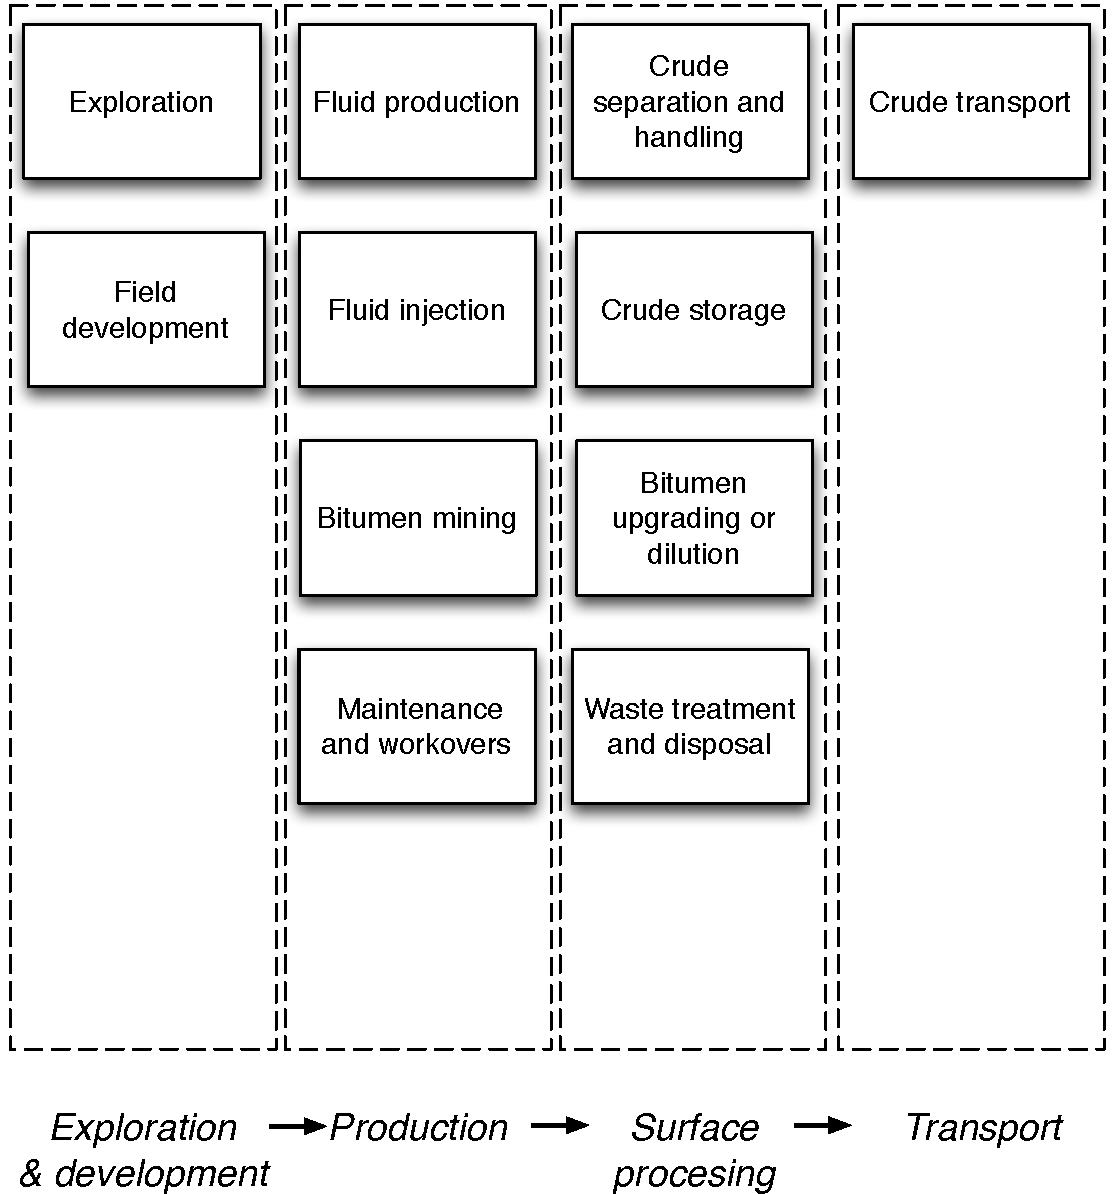
\includegraphics[width=0.85\columnwidth]{images/Flow_sheet_v4.pdf}
\caption{Schematic chart showing included stages within OPGEE.}
\label{fig:OPGEE_stages}
\end{figure}


\subsection{Spreadsheet structure}

OPGEE is modular in structure, with interlinked worksheets representing each production stage. Within each major production stage, a number of activities and processes occur (e.g., fluid production or fluid injection). Calculations take place sequentially and are numbered in a hierarchical fashion (see Box 2.1 for explanation of pointers to the model in this document). 

\subsection{Modeling detail and default specifications}

OPGEE models oil production emissions in more detail than previous LCA models. For example, the energy consumed in lifting produced fluids (oil, water, and associated gas) to the surface is computed using the fundamental physics of fluid lifting, accounting for friction and pump efficiencies. 

Increased modeling detail results in an increase in the number of model parameters. All required inputs to OPGEE are assigned default values that can be kept as is or changed to match the characteristics of a given oil field or marketable crude oil blend. If only a limited amount of information is available for a given facility, most input values will remain equal to defaults. In contrast, if detailed field-level data are available, a more accurate emissions estimate can be generated.

For some processes and sub-processes, correlations or relationships are developed for defaults, which we call "smart defaults". For example, the amount of water produced with oil (water-oil-ratio, or WOR) affects the energy consumed in lifting, handling, and separating fluids. If the WOR is known, it can be inputed directly. However, in some regions, water production is not reported, so OPGEE includes a statistical relationship for water production as a function of reservoir age (see Section \ref{WORSmartDefault} for a description of the analysis underlying this smart default).

A workflow for updating and improving the data basis and accuracy of an emissions estimate using OPGEE is shown in Figure \ref{fig:OPGEE_flow}. This workflow represents one possible way that OPGEE could be used.


\begin{figure}[t]
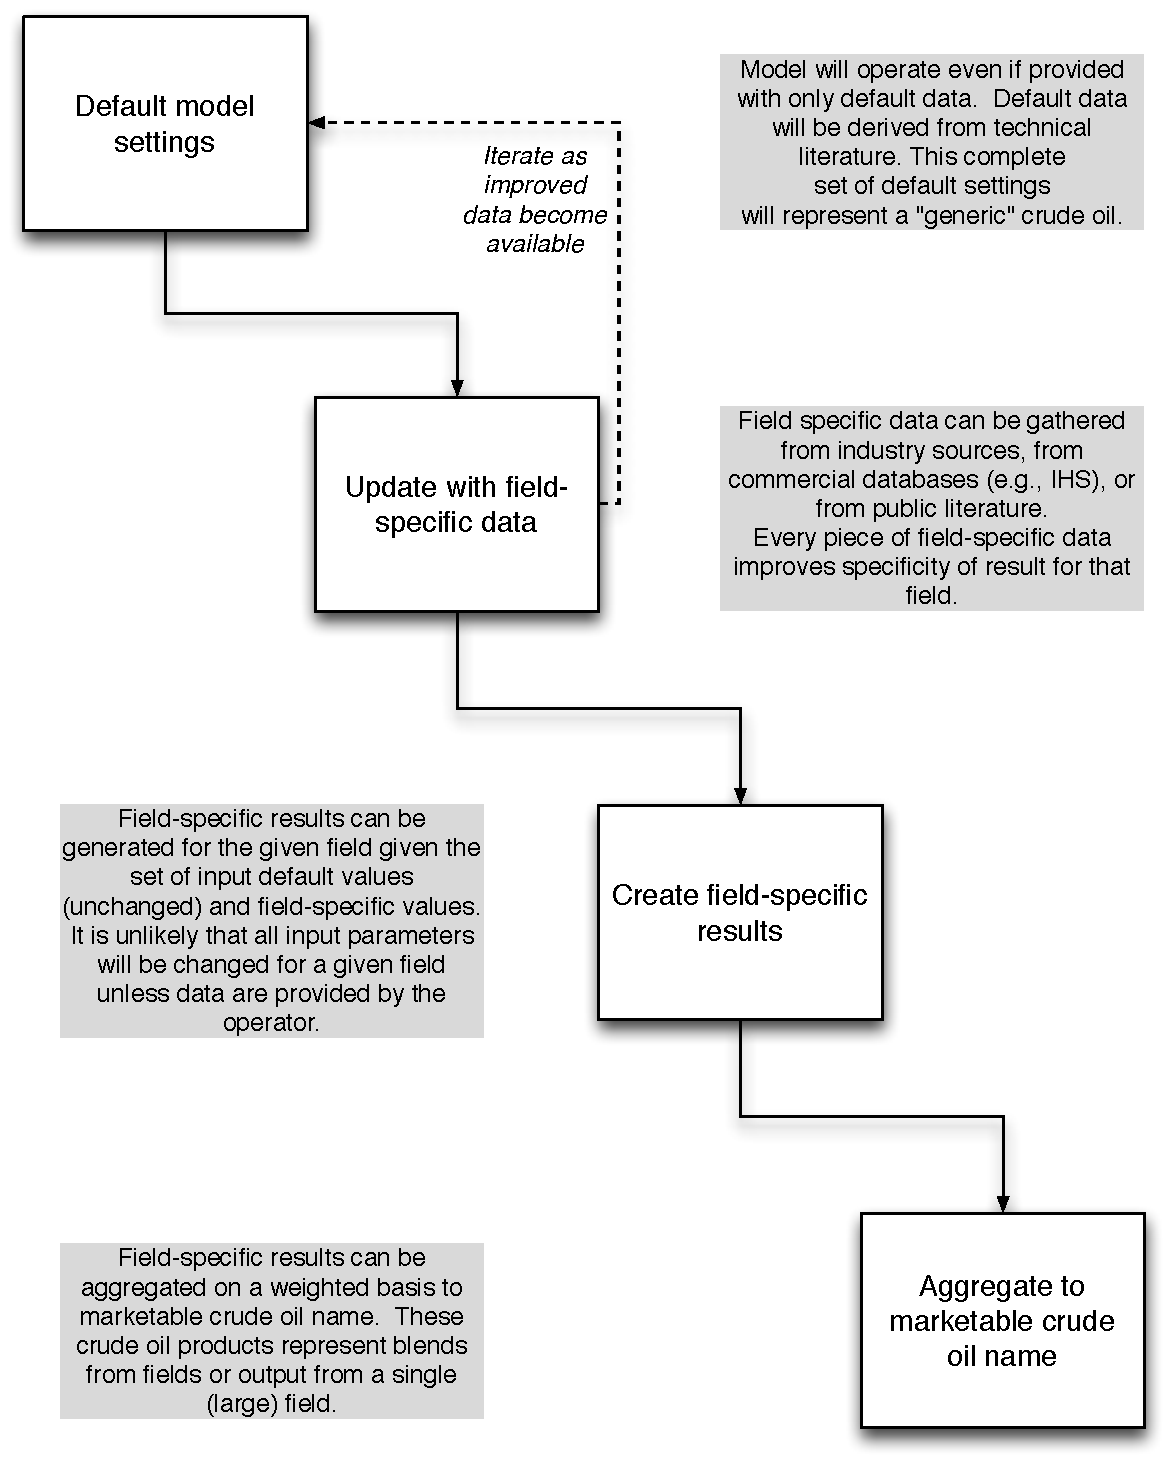
\includegraphics[width=0.8\columnwidth]{images/Flow_chart.pdf}
\caption{Proposed workflow for improving emissions estimates using OPGEE.}
\label{fig:OPGEE_flow}
\end{figure}




\subsection{Emissions sources classification}

Each process stage or sub-process in OPGEE can result in a variety of emissions sources. For example, the \sheet{Drilling \& Development} process stage includes the terrestrial drilling sub-process. Terrestrial drilling could include the following emissions sources:
\begin{itemize}
\item Combustion emissions from drilling rig prime mover;
\item Flaring emissions from drilling rig;
\item Vents and other upset emissions from drilling rig;
\item Combustion emissions from work performed in land clearing and site preparation;
\item Biogenic emissions from ecosystem disturbance during development;
\item Embodied emissions in cement and casing;
\item Embodied emissions in other consumable materials (e.g., fracturing sand)
\end{itemize}
Note that these emissions sources are of significantly different magnitude and have different causation and potential methods of mitigation. In total, over 100 emissions sources are classified in OPGEE \version \, across all process stages (e.g., all included processes and sub-processes). See Appendix \ref{sec:app_sources_classification} for a complete tabulation and classification of emissions sources.  Model coverage is also shown in the \sheet{Model Coverage} tab of OPGEE \version.



\subsection{Emissions source significance cutoffs}

It would be infeasible (and counter-productive) to attempt to estimate the magnitude of every emissions source listed in Appendix \ref{sec:app_sources_classification}. Fortunately, a small number of emissions sources will result in most of the emissions from petroleum production operations. 

For this reason, emissions sources included in the OPGEE system boundary are classified by estimated emissions magnitude. These emissions magnitudes are meant to represent \emph{possible} emissions magnitudes from a source, not the actual emissions that would result from that source for any particular field. An order-of-magnitude estimation approach is used, with each source assigned a rating in ``stars'' from one-star (*) to four-star (****) corresponding to 0.01 to 10 g CO$_2$ eq.\ per MJ of crude oil delivered to the refinery gate. These classifications are explained in Table \ref{tab:emissions_significance}.

Emissions estimated to be one-star emissions (*) are not modeled in OPGEE due to insignificant magnitude. Since these small sources are known to have non-zero emissions, they are included in the overall emissions estimate by including a ``small sources'' term. \marginnote{Results 2.8} Two-star (**) sources are included simply or are included in the small sources term. Often, two-star sources are minor in magnitude, but are modeled due to the need to model the physics and chemistry of crude oil production and processing.\footnote{No strict criteria exist to determine the inclusion or exclusion of two-star sources. Modeler judgement is applied to determine the need for modeling these sources.} Three-star (***) sources are explicitly modeled in OPGEE. Four-star sources (****) are modeled in detail with stand-alone modules to allow variation and uncertainty analysis. 

\begin{table}
\begin{scriptsize}
\caption{Emissions classification, order of magnitude emissions, and significance description.}
\label{tab:emissions_significance}
\begin{tabular}{p{0.07\columnwidth}p{0.12\columnwidth}p{0.74\columnwidth}}
\toprule
Class & Est. mag. [gCO$_2$/MJ] & Description \\
\midrule
* & 0.01 & Minor emissions sources not worthy of further study or estimation. This is the most common classification. One-star emissions are accounted for by adding a value for miscellaneous minor emissions.\\
** & 0.1 & Minor emissions sources that are often neglected but may be included for physical completeness.\\
*** & 1 & Sources that can have material impacts on the final GHG estimate, and therefore are explicitly modeled in OPGEE. \\
**** & 10 & Sources that are large in magnitude (though uncommon). Examples include steam production for thermal oil recovery and associated gas flaring. These sources are significant enough to require their own dedicated OPGEE modules.\\
\bottomrule 
\end{tabular}
\end{scriptsize}
\end{table}


\subsection{Data sources}

Because of the need for transparent data basis, OPGEE uses data from a variety of technical reference works. For example, emissions factors are derived from standard engineering references from the American Petroleum Institute (API) and Environmental Protection Agency (EPA) \cite{EPA1995, Shires2004}. A large number of technical references, journal articles, and fundamental data sources have been consulted during the construction of OPGEE, including: 
\begin{itemize}
\item Exploration and drilling \cite{Shires2004, Azar2007, Devereux1998, Gidley1989, Lapeyrouse2002, Mitchell2006, Mitchell2011, Wilson1999}
\item Production and surface separations \cite{Shires2004, EPA1995, API1991, API1993a, API1995a, API1996b, API1998a, API2003, API2006, API2008a, API2008b, API2009a, API2009b, API2009c, API2009d, Arnold2007, Chilingarian1987, Chilingarian1989, Cholet2000, Clegg2007, Fanchi2007, GPSA2004, Holstein2007a, Holstein2007b, Leffler2006, Manning1991, Manning1995, Stewart2008, Stewart2009, Stewart2011, Takacs1993, Takacs2003}
\item Secondary and tertiary recovery \cite{Craig1993, Jarrell2002, Prats1985, Rose1989, Warner2007, Green1998}
\item Water treatment and waste disposal \cite{Wilson1999, Manning1995, Stewart2011, Khatib2002, Neff2007, Reed1996, Veil2004}
\item Venting, flaring, and fugitive emissions \cite{API1991, API1993a, API1995a, API1996b, API1998a, API1998b, API1998c, API2003, API2006, API2008a, API2008b, API2008c, API2009a, API1993b, API1995a, API2009e}
\item Petroleum transport and storage \cite{API2006, GPSA2004, API1993b, API1995b, API1997, API2009a, Mcallister2009, Miesner2006, Szilas1985}
\end{itemize}

%%%%%%%%%%%%%%%%%%%%%%%%%%%%%%%%%%%%%%%%%%%%%%%%
\clearpage


%%%%%%%%%%%%%%%%%%%%%%%%%%%%%%%%%%%%%%%%%%%%%
%%%%%%%%%%%%%%%%%%%%%%%%%%%%%%%%%%%%%%%%%%%%%
%%%%%%%%%%%%%%%%%%%%%%%%%%%%%%%%%%%%%%%%%%%%%

\chapter{User guide}

OPGEE is divided into four types of worksheets: (1) input sheets, (2) process stage worksheets, (3) supplementary worksheets, and (4) output gathering worksheets.


\clearpage

%%%%%%%%%%%%%%%%%%%%%%%%%%%%%%%%%%%%%
\section{Input and output worksheets}

\paragraph{\sheet{Inputs} worksheet}

Data are entered on the input worksheet in OPGEE \version. This worksheet is labeled \sheet{Inputs} and is colored green.  The user  can input a simplified set of $\approx$ 50 data inputs on the \sheet{Inputs} worksheet. Data for hundreds of fields can be entered on the \sheet{Inputs} sheet. The data entered by the user are stored on the \sheet{Inputs} sheet without modification, so the \sheet{Inputs} sheet can be used to compile and store data for a variety of operations.

OPGEE \version\, is run from the \sheet{Inputs} sheet.  The user enters the starting field of analysis and the ending field of analysis and presses the ''Run Assessment'' button.  See more detail about using the model below.

\paragraph{\sheet{Results} worksheet}
Results generated by OPGEE are stored in the \sheet{Results} worksheet. \sheet{Results} compiles information for the analyzed crude oils, and represents the holding sheet for all changed parameters that are adjusted by OPGEE algorithms.  The \sheet{Results} sheet should be the place where the user obtains final results for runs of a particular field.

Note that the \sheet{Results} worksheet is the repository of all results for fields that are analyzed as part of a multi-field assessment.  


\clearpage

%%%%%%%%%%%%%%%%%%%%%%%%%%%%%%%%%%%%%
\section{Field summary worksheets}

Field summary worksheets present information about the field most recently analyzed. Flows for the field under analysis are presented and organized in the \sheet{Flow Sheet} worksheet. Process stage calculations are compiled into summed energy consumption (including energy co-production credits) and summed GHG emissions (including any offsets from co-produced energy).  Output worksheets have brown-colored tabs.


\paragraph{\sheet{Active Field} worksheet}
The \sheet{Active Field} worksheet presents summary inputs and results in tabular and graphical form for the most recently processed field. After a run involving multiple fields, \sheet{Active Field} retains the data from last field assessed and does not save results for prior fields. \sheet{Active Field} allows for detailed tracking and analysis of the results for an individual field. The \sheet{Active Field} worksheet is described in Section \ref{sec:active_field}.  

The \sheet{Active Field} worksheet serves as a holding place for information on the field currently under analysis during a particular OPGEE run, and logic on the sheet applies many of the ``smart defaults'' defined below.  For this reason, the \sheet{Active Field} worksheet should not be modified by the user (at least without great care). 

\paragraph{\sheet{Flow Sheet} worksheet}

The \sheet{Flow Sheet} worksheet tracks all flows into and out of each process unit. All flows for a set of tracked liquid, gas, and solid products are tracked from primary extraction from geologic deposits until final disposition.  The \sheet{Flow Sheet} is the key sheet for navigating to process level calculations.


\paragraph{\sheet{Energy Consumption} worksheet}
The \sheet{Energy Consumption} worksheet gathers data on energy consumption for sub-processes from all process worksheets. Each main process worksheet is included in the gathering table. All energy consumed is summed by type across all stages. This gross consumption is used to compute net consumption and energy imports and exports. The \sheet{Energy Consumption} worksheet is described in Section \ref{sec:energy_consumption} 

\paragraph{\sheet{GHG Emissions} worksheet}
The \sheet{GHG Emissions} worksheet takes the energy quantities consumed in each stage and converts them to emissions using emissions factors. It also gathers any emissions associated with land use change and VFF emissions. Emissions are computed as gCO$_2$eq./d. The \sheet{GHG Emissions} worksheet is described in Section \ref{sec:GHG_emissions}.



\clearpage

%%%%%%%%%%%%%%%%%%%%%%%%%%%%%%%%%%%%%
\section{Process stage worksheets}
Process stage worksheets form the core of OPGEE, and are where most model calculations occur. These worksheets have red-colored tabs.

Process stage worksheets are most easily accessed through the \sheet{Flow Sheet} tab, where each process unit or process stage is represented by a box with a ``go to'' button. Press the ``go to'' button for each process unit to jump to that process unit to examine calculations.

\clearpage

%%%%%%%%%%%%%%%%%%%%%%%%%%%%%%%%%%%%%
\section{Supplementary worksheets}

Supplementary worksheets support calculations throughout OPGEE, including: calculating intermediate outputs in the process stage worksheets, compiling output in the gathering worksheets, and calculating results in the \sheet{Active Field} worksheet. Supplementary worksheets have blue-colored tabs.

\paragraph{\sheet{Electricity} worksheet} This worksheet determines the offsite electricity mix and calculates the energy consumption in onsite electricity generation (other than electricity co-generated with steam). The \sheet{Electricity} worksheet is described in Section \ref{sec:electricity}.

\paragraph{\sheet{Drivers} worksheet} This worksheet provides a database of energy consumption for different types and sizes of prime movers (gas and diesel engines, gas turbines and electric motors). The \sheet{Drivers} worksheet is described in Section \ref{sec:drivers}.

\paragraph{\sheet{Fuel Cycle} worksheet} This worksheet retrieves and calculates the fuel cycle energy consumption and GHG emissions for the calculation of credits/debits from fuel exports/imports. The \sheet{Fuel Cycle} worksheet is described in Section \ref{sec:fuel_cycle}.

\paragraph{\sheet{Emission Factors} worksheet} This worksheet retrieves and builds emissions factors for the calculation of combustion and non-combustion GHG emissions from energy use and losses. The \sheet{Emissions Factors} worksheet is described in Section \ref{sec:emissions_factors}.

\paragraph{\sheet{Venting \& Fugitives} worksheet} This worksheet calculates in detail the GHG emissions associated with Venting and fugitives. The \sheet{Venting \& Fugitives} worksheet is described in Section \ref{sec:VF}.

\paragraph{\sheet{Fuel Specs} worksheet} This worksheet provides fuel specifications required for OPGEE calculations. The \sheet{Fuel Specs} worksheet is described in Section \ref{sec:data_inputs}.

\paragraph{\sheet{Inputs} worksheet} This worksheet provides other needed data inputs such as conversion factors and steam enthalpies. The \sheet{Input Data} worksheet is described in Section \ref{sec:data_inputs}.

\vspace{0.1in}


\clearpage

%%%%%%%%%%%%%%%%%%%%%%%%%%%%%%%%%%%%%
\section{Structure of process stage worksheet}
Most process stage worksheets are divided into four main sections: (1) Flows, (2) Inputs, (3) Calculations, (4) Outputs. 

\subsection{Flows} 
The flows section of each process stage worksheet tracks flows into the process and flows out of the process. Flows are denominated in tonnes per day (with the exception of electricity, denominated in MWh per day).

Flow cells are bold if directly computed in that sheet, and standard weight font if drawn directly from the flow table (for example, as an input to the process unit.

\begin{figure}[t]
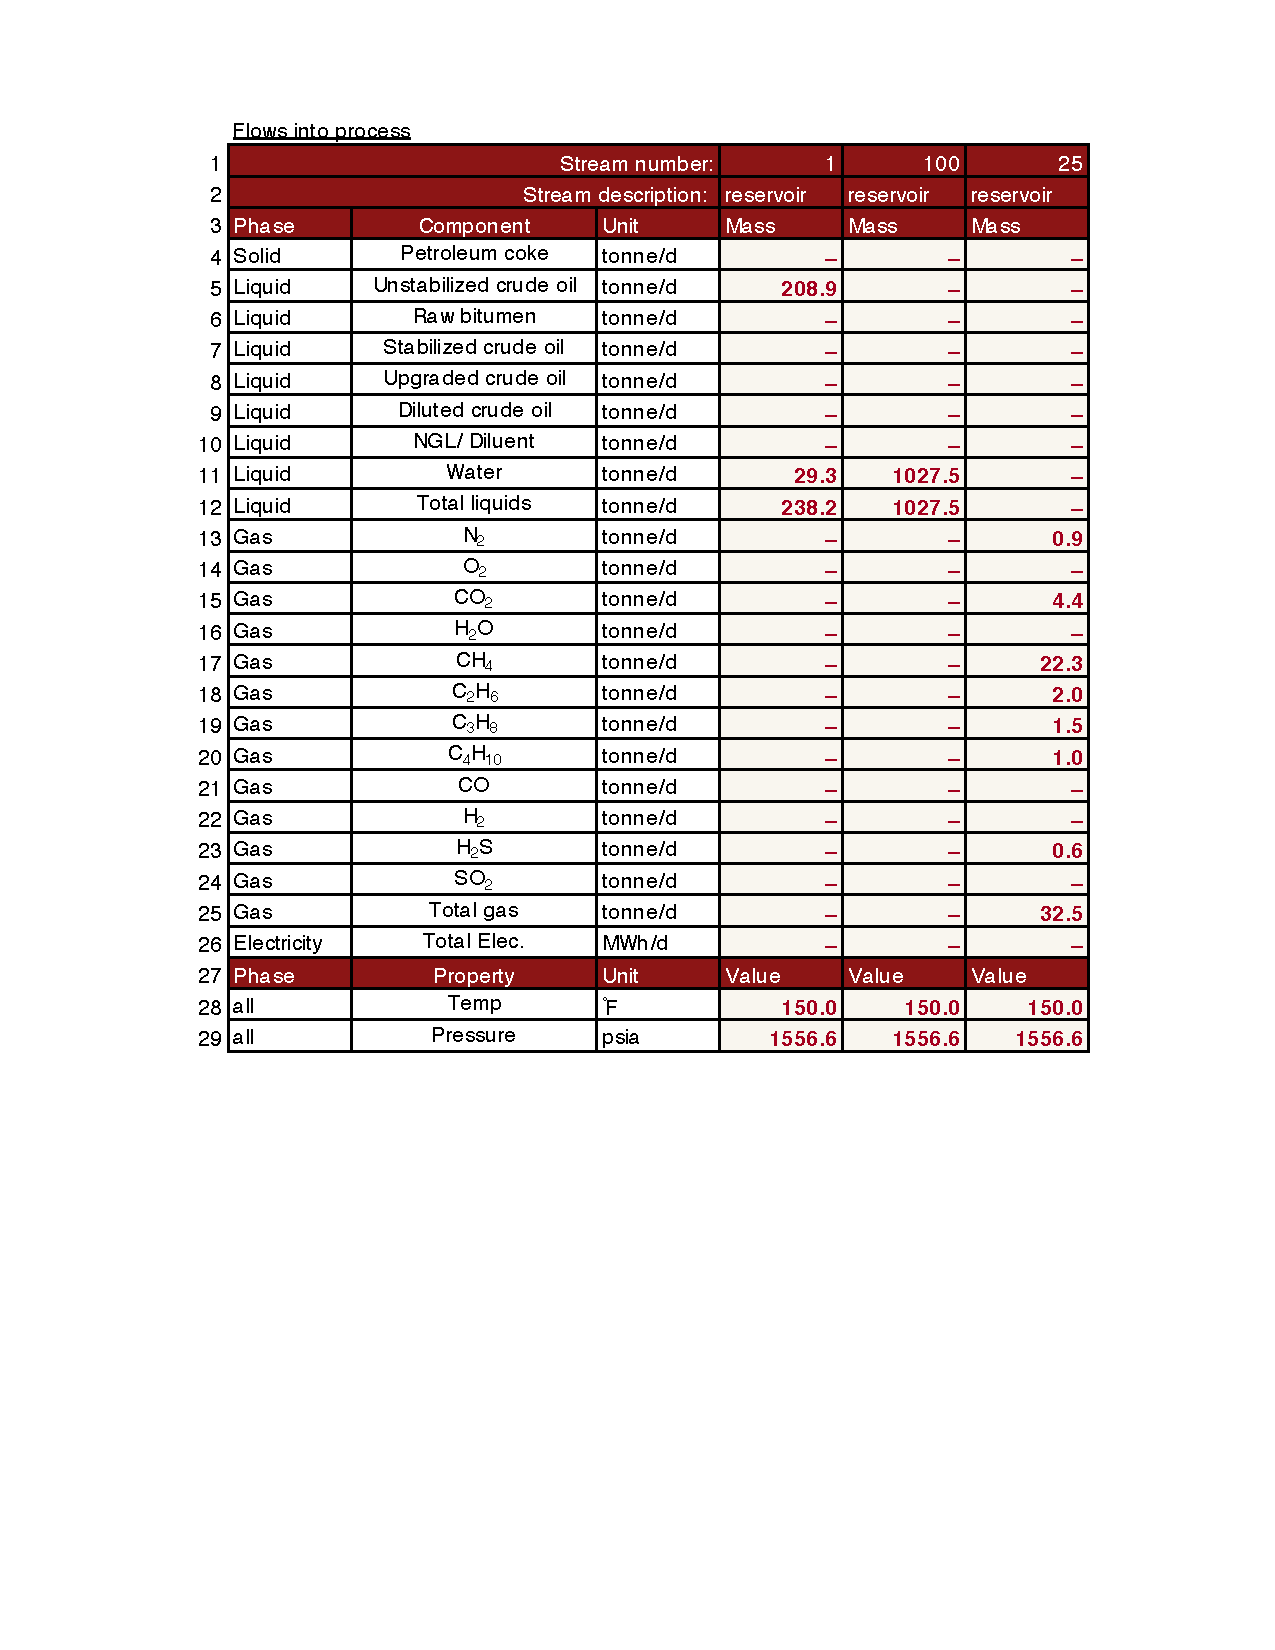
\includegraphics[width=0.8\columnwidth]{images/FlowTable.pdf}
\caption{Example flow table in OPGEE 3.0  Flows are segregated by phase (solid, liquid, gas) or type (electricity). Fundamental properties of each stream, including temperature and pressure, are recorded a the bottom of each flow.}
\label{fig:FlowTable}
\end{figure}

\subsection {Inputs}

The input data section is where the user enters the input parameters (e.g., API gravity, production volume). Inputs are divided into three types:
\begin{enumerate}
\item Key parameters
\item Secondary parameters
\item Parameters defined on other sheets
\end{enumerate}

Key parameters are drawn directly from the \sheet{Active Field} sheet.  Secondary parameters are parameters that are used in the calculations in a process stage sheet, but are not fundamental enough to warrant inclusion on the \sheet{Active Field} sheet.  Parameters defined on other sheets include anything previously defined, computed, or entered as a secondary parameters on another worksheet.

The input section of each worksheet has two data columns: \emph{User} and \emph{Default}, in columns M and N, respectively. The cells within the \emph{User} column are the active cells, used to generate results in the calculations section. The cells within the \emph{Default} column are used for reference, bookkeeping of default values, and generating defaults using correlations based on field data. 

\subsection{Calculations}
Below the input data section is the calculations section of a worksheet, where intermediate model outputs are calculated. These intermediate outputs are summarized and compiled by the gathering worksheets to provide the overall energy and emissions measures compiled in the \sheet{Outputs} worksheet.

\subsection{Outputs}
The outputs section holds the summary results in terms of energy use and emissions that are later collected in the summary sheets.


\subsection{Types of model cells}
Four main types of cells exist in the calculation columns M and N: \emph{User Free}, \emph{User Locked}, \emph{Default Free}, \emph{Default Locked} (See Figure \ref{fig:Cell_types_SS}). As might be expected, locked cells should not be changed.\footnote{Note: `locked' cells are not locked via \emph{Excel} password-protected locking mechanism, so they can be changed if desired by the user. However, this should be done with care, as the model can easily be rendered inoperable.} This is typically because locked cells contain formulas that draw on other cells and therefore should no t be changed. ``User Free'' cells are cells that allow entry of user data. 

\begin{figure}[t]
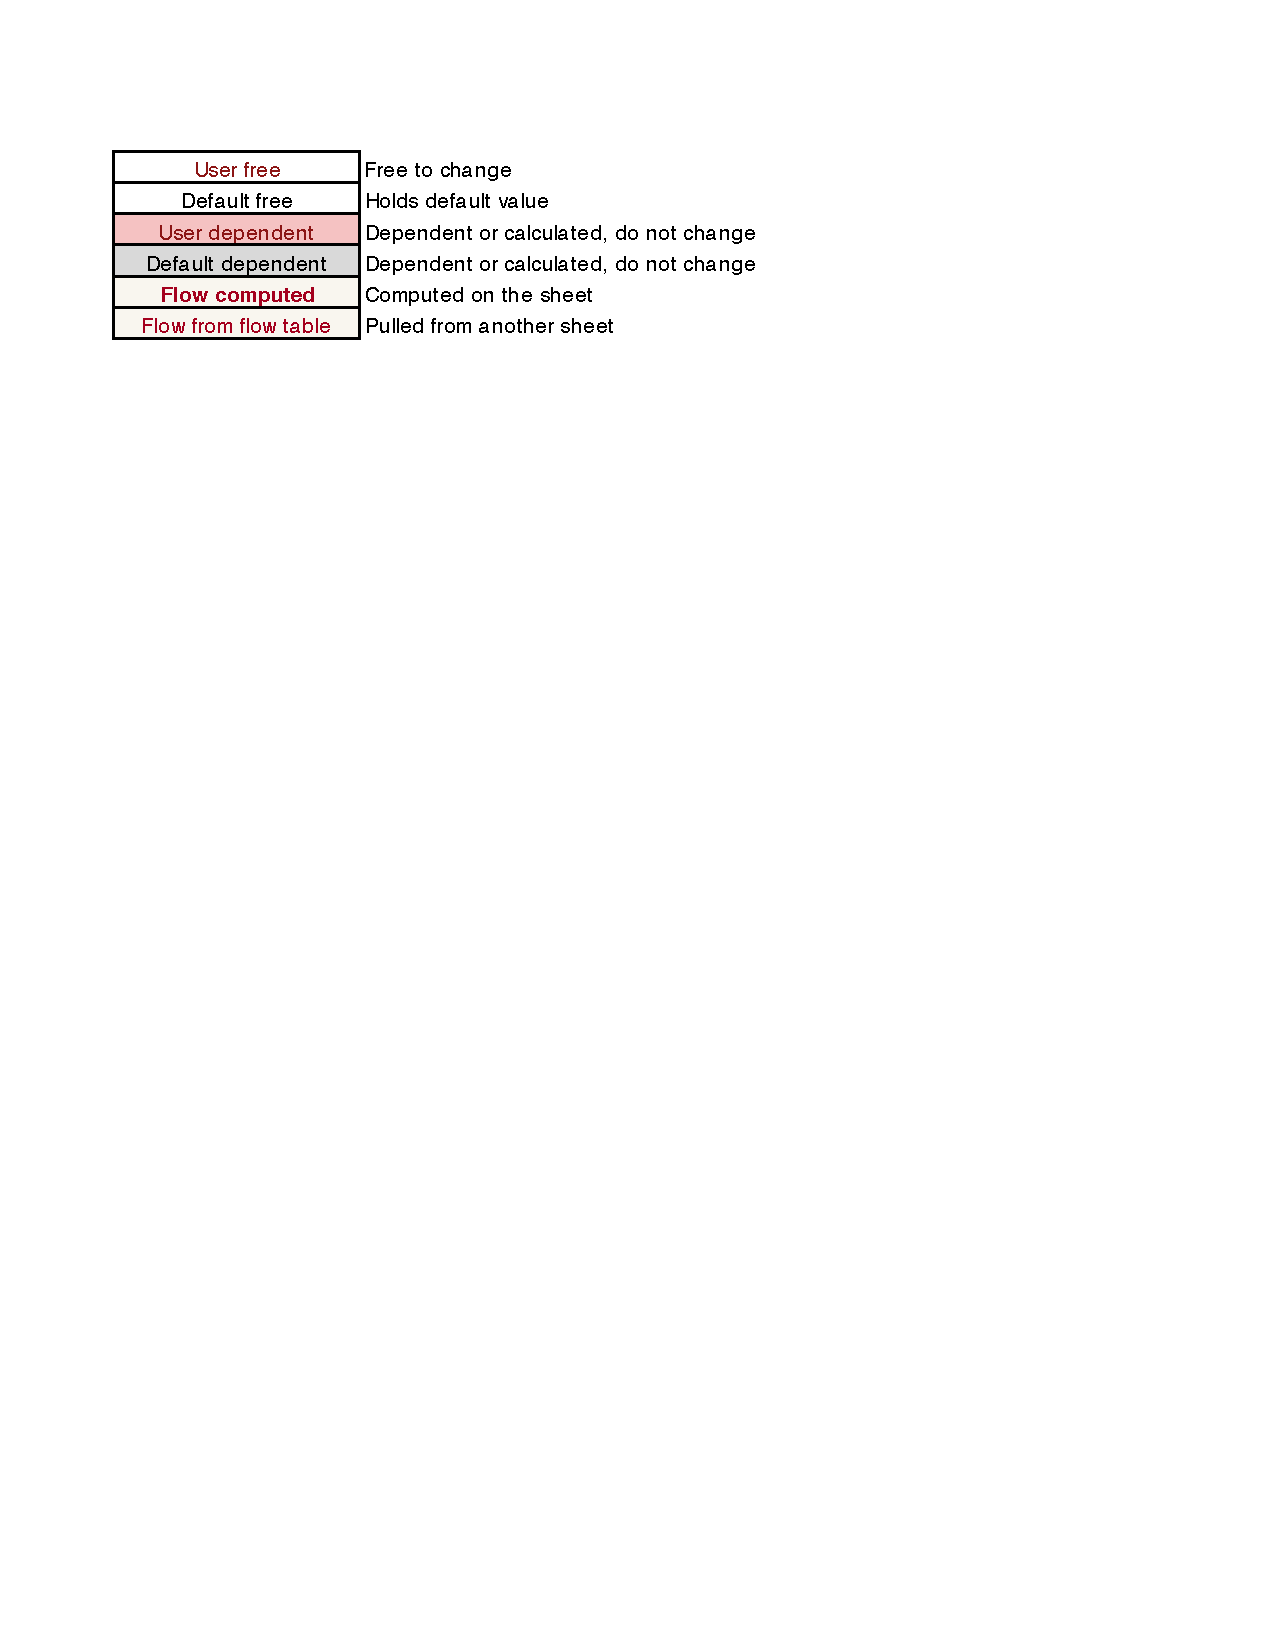
\includegraphics[width=0.8\columnwidth]{images/CellTypes.pdf}
\caption{Types of cells. \emph{User Free} and \emph{Default Free} cells can be changed, while \emph{Locked} cells should not be changed due to possibility of compromising model functionality. Flow sheet cells are either calculated in place or looked up from the large flow table.}
\label{fig:Cell_types_SS}
\end{figure}


\clearpage

%%%%%%%%%%%%%%%%%%%%%%%%%%%%%%%%%%%%%
\section{Working with OPGEE}

This section explains how to work with OPGEE. Box 2.1 shows how to best use this documentation in concert with the OPGEE model itself.

\subsection{Primary interaction}\label{sec:primary_interaction}

The easiest way to use OPGEE (which this document calls ``primary'' interaction) is to input key parameters for a field or set of fields to the \sheet{Inputs} sheet. These key parameters have the following characteristics:
\begin{itemize}
\item They have a significant effect on the GHG emissions from an oil and gas operation;
\item They vary significantly across different operations and therefore could cause variability between different fields or projects;
\item They are likely to be measured or are well-understood by operators.
\end{itemize}
The list of key inputs is a relatively small list of important factors. Other factors excluded from this list are left to process worksheets.


\begin{figure}
\fcolorbox{black}{gray!20}{ 
\parbox{\tw}{\boxtitle{Box 2.1: Using OPGEE documentation and model together \vspace{0.05in}} \\ 
\begin{small}
OPGEE model documentation aligns with the model itself. Pointers to the model are contained in the right-hand margin of the model documentation in red, italic text. For example, the bubblepoint solution gas oil ratio is computed in row 65 of the \sheet{Reservoir} worksheet, and would be referred to in the right-hand margin as \emph{\color{stanford}Reservoir Row 65}
\end{small}
}} 
\label{box:dochints}
\end{figure}

\subsubsection{Controls on the \sheet{Inputs} worksheet}

The \marginnote{Inputs 1.1 - 1.8} \sheet{Inputs} worksheet is where key field parameters are entered for each field to be analyzed (see Figure \ref{fig:Inputs}). These key parameters are explained below.

\paragraph{Production methods} Controls to turn on or off production methods \marginnote{Inputs 1.1} including downhole pump, water reinjection, gas reinjection, water flooding, gas lifting, gas flooding, steam flooding, oil sands mine (integrated with upgrader), and oil sands mine (non-integrated with upgrader).
\begin{itemize}
\item Downhole pump: This option is used to allow production when the naturally-occurring energy of the reservoir does not suffice to produce fluids at a desired wellhead pressure.
\item Water reinjection: This option is used when injecting a fraction of the produced water. This option does not apply if the amount of water injected is more than the amount of water produced after treatment.
\item Gas reinjection: This option is used when injecting a percentage of the amount of gas produced. This option does not apply if the amount of gas injected is more than the amount of gas remaining after processing and VFF losses. The remaining gas is shown in the \sheet{Gas Balance} worksheet.
\item Water flooding: This option is used when injecting an amount of water which is more than the amount of water produced. The amount of water injected is determined by the injection ratio (given in bbl water/bbl oil) and the fraction of water produced to reinjection/flooding must be set to 1.0. \textbf{The option of water reinjection must be turned OFF when the option of water flooding is turned ON.} 
\item Gas lifting: This option is used when gas is not injected into the reservoir, but injected into production string to reduce the pressure at the reservoir interface and induce production from the reservoir.
\item Gas flooding: This option is used when injecting an amount of natural gas which is more than the amount of gas remaining after processing. The amount of gas injected is determined by the injection ratio (given in scf/bbl oil) and the fraction of remaining natural gas to reinjection must be set to 1.0. Alternately, this option can also be used when modeling EOR by flooding of nitrogen and carbon dioxide. \textbf{The option of gas reinjection must be turned OFF when the option of gas flooding is turned ON AND natural gas is selected as the flood gas.}
\item Steam flooding: This EOR option is used when steam is injected to extract heavy crude oil. When this option is turned ON, steam-to-oil ratio (SOR) is needed to be entered or OPGEE will use its SOR default. The option of offshore field should be turned OFF when the option of steam flooding is turned ON.
\item Oil sands mine (integrated or non-integrated with upgrader): The mining projects are mostly related to the Canadian oil sands. see section \,\ref{sec:bitumen_mining} for more details. 
 
\end{itemize}

\paragraph{Field properties} Field properties, including field location, \marginnote{Inputs 1.2} field name, field age, field depth, oil production volume, number of producing wells, number of water injecting wells, production tubing diameter, productivity index, average reservoir pressure, average reservoir temperature, and whether the field is onshore (0) or offshore (1).

\paragraph{Fluid properties} A variety of fluid properties, including \marginnote{Inputs 1.3} API gravity of crude oil and composition of produced associated gas (N$_2$, CO$_2$, C$_1$, C$_2$, C$_3$, C$_4+$, and H$_2$S molar concentrations). 

\paragraph{Production practices} A variety of production practices or \marginnote{Inputs 1.4} operating ratios. These include gas-to-oil ratio (GOR), water-to-oil ratio (WOR), water-injection ratio, gas lifting injection ratio, gas flooding injection ratio, the choice of flood gas (natural gas, N$_2$, and CO$_2$), carbon dioxide enhanced oil recovery (CO$_2$-EOR) related parameters (the percentage of the total injected CO$_2$ that is newly acquired, the source of CO$_2$, and the percentage of the CO$_2$ sequestration credit assigned to the oilfield), steam-to-oil ratio (SOR), fraction of required electricity generated on site, fraction of remaining gas reinjected, fraction of water produced reinjected, fraction of steam generation via co-generation and volume fraction of diluent. WOR, GOR, and SOR are common parameters and self explanatory. Other less common parameters are explained below.
\begin{itemize}

\item Water injection ratio: The ratio of the amount of water injected in water flooding to the amount of oil produced. This is required only when the option of water flooding is turned ON.
\item Gas lifting injection ratio: The ratio of the amount of gas injected for lifting to the amount of liquid (water + oil) produced. The amount of gas injected for gas lifting \textbf{does not} include gas injected into the reservoir. This is required only when the option of gas lifting is turned ON. 
\item Gas flooding injection ratio: The ratio of the amount of gas injected in gas flooding to the amount of oil produced. This is required only when the option of gas flooding is turned ON.
\item Flood Gas: The choice flood gas (natural gas, N$_2$, CO$_2$). This is required only when the option of gas flooding is turned ON.
\item Percentage of total CO$_2$ injected that is newly acquired: The total amount of CO$_2$  injected consists of the sum of recycled CO$_2$ (that was previously injected, produced, and separated) and newly acquired CO$_2$ that is being injected for the first time. This is required only if the option of gas flooding is turned ON and CO$_2$ is the selected flood gas.
\item Source of CO$_2$: CO$_2$ can be acquired either from natural subsurface reservoirs or captured from anthropogenic sources such as power plants. This is required only if the option of gas flooding is turned ON and CO$_2$ is the selected flood gas.
\item Percentage of sequestration credit assigned to the oilfield: Greenhouse gas emissions-related legislation may allow the oilfield to claim a sequestration credit for CO$_2$ sequestered during CO$_2$-EOR operations. If such a credit applies, then this parameter controls the proportion assigned to the oilfield. This is required only if the option of gas flooding is turned ON and CO$_2$ is the selected flood gas.
\item Fraction of required electricity generated onsite: This parameter determines the fraction of the electricity required that is generated onsite not including electricity co-generation with steam generation. The fraction entered can be greater than 1.0, designating electricity export to the grid.
\item Fraction of remaining gas reinjected: This parameter determines the fraction of gas remaining that is reinjected into the reservoir. In the case of methane gas flooding this fraction must be equal to 1.0 (the amount of gas injected is more than the amount of gas remaining).
\item Fraction of water produced reinjected: This parameter determines the fraction of water produced after treatment that is reinjected into the reservoir. In the case of water flooding this fraction must be equal to 1.0 (the amount of water injected is more than the amount of water produced).
\item Fraction of steam generation via co-generation: OPGEE allows the modeling of steam generation for thermal EOR with or without electricity co-generation. This parameter determines the share of steam generation via co-generation of electricity. 

\end{itemize}


\paragraph{Processing practices} Variables which represent \marginnote{Inputs 1.5} the use of heater/treaters and stabilizer columns during oil phase separation, upgrader type, the choice of associated gas processing (AGR, dehydrator, demethanizer, and CO$_2$ EOR-related processing options), the ratio of gas flared to oil produced, and the ratio of gas vented to oil produced. Some parameters are explained below.

\begin{itemize}
\item Heater/treater: Binary variables (0 or 1) are used to determine the use of a heater/treater in the oil-water separation process. 1 is used to turn ON the heater/treater and 0 is used to turn OFF the heater/treater. More detailed choices for heater/treaters are made in the \sheet{Surface Processing} worksheet.
\item Stabilizer column: Binary variables (0 or 1) are used to determine the use of a stabilizer column in the oil-gas separation process. 1 is used to turn ON the stabilizer column and 0 is used to turn OFF the stabilizer column. The stabilizer column is defined in section \,\ref{sec:crude_stabilization}. 
\item Associated gas processing path: A set of 7 gas processing configurations are allowed to be chosen by setting value in this cell from 1 to 8. These options range from no gas processing (1) to extensive gas processing and CO$_2$ separation via cryogenic separation (8).  Significant detail is provided on these gas processing paths below.
\item Ratio of flaring to oil production: This is the ratio of gas flared to oil produced. 
\item Ratio of venting to oil production: This is the ratio of gas vented (not including operational venting or default leaks) to oil produced. \textbf{This ratio only includes venting used for gas disposal, as an alternative to flaring. It does not address normal operational vents and leaks}. Other default leaks are accounted in the \sheet{Venting \& Fugitives} worksheet.
\item Volume fraction of diluent: In some cases heavy crude is diluted after production using light hydrocarbons. This parameter determines the fraction of diluent or natural gas liquid (NGL) in diluted crude. The default case is the minimum NGL blend as determined by user inputs. The process model produces NGL in the demethanizer (if applicable), a fraction of which is blended as specified in the \sheet{Surface Processing} worksheet. 
\end{itemize} 

\paragraph{Land use impacts} Parameters that determine the \marginnote{Inputs 1.6} GHG emissions from land use change, including ecosystem carbon richness and relative disturbance intensity. 
\begin{itemize}
\item Ecosystem carbon richness: Ecosystem carbon richness controls the amount of carbon emissions per unit of disturbed land, and varies from semi-arid grasslands (low potential carbon emissions) to forested (high potential carbon emissions). 
\item Field development intensity: The intensity of development can be chosen to be low, medium, or high. High intensity development resembles California thermal EOR operations, well production and injection wells are drilled on tight spacing. Low intensity development resembles conventional natural gas development or directional drilling from centralized drill pads, where the land disturbed per well is small.
\end{itemize}

\paragraph{Crude oil transport} Parameters which determine transport \marginnote{Inputs 1.7} modes and distances. This includes the fraction of crude oil transported by each mode of transport and the transport distance (one way) of each mode. The total fraction of all modes may exceed 1.0 because more than one transportation leg may be involved for transporting the crude oil from field to refinery.


\paragraph{Small emissions sources} An added term to account for all \marginnote{Inputs 1.8} emissions sources that are not explicitly included in OPGEE through calculations. Tables \ref{tab:exploration_sources} through \ref{tab:transport_sources}, as well as the \sheet{Model Organization} worksheet in OPGEE, describe which sources are explicitly included in the model. All sources that are not explicitly included are deemed to small to model, and are included in the small emissions sources term.
\vspace{0.1in}

Parameters for multiple fields can be entered at a single time.
After entry into \sheet{Inputs}, values for key parameters are propagated to other worksheets as needed for calculations. Therefore, if a key parameter (such as API gravity) is to be changed, it \textbf{must} be changed on the front \sheet{Inputs} worksheet so that it is changed identically in all calculations. 



\begin{figure}[t]
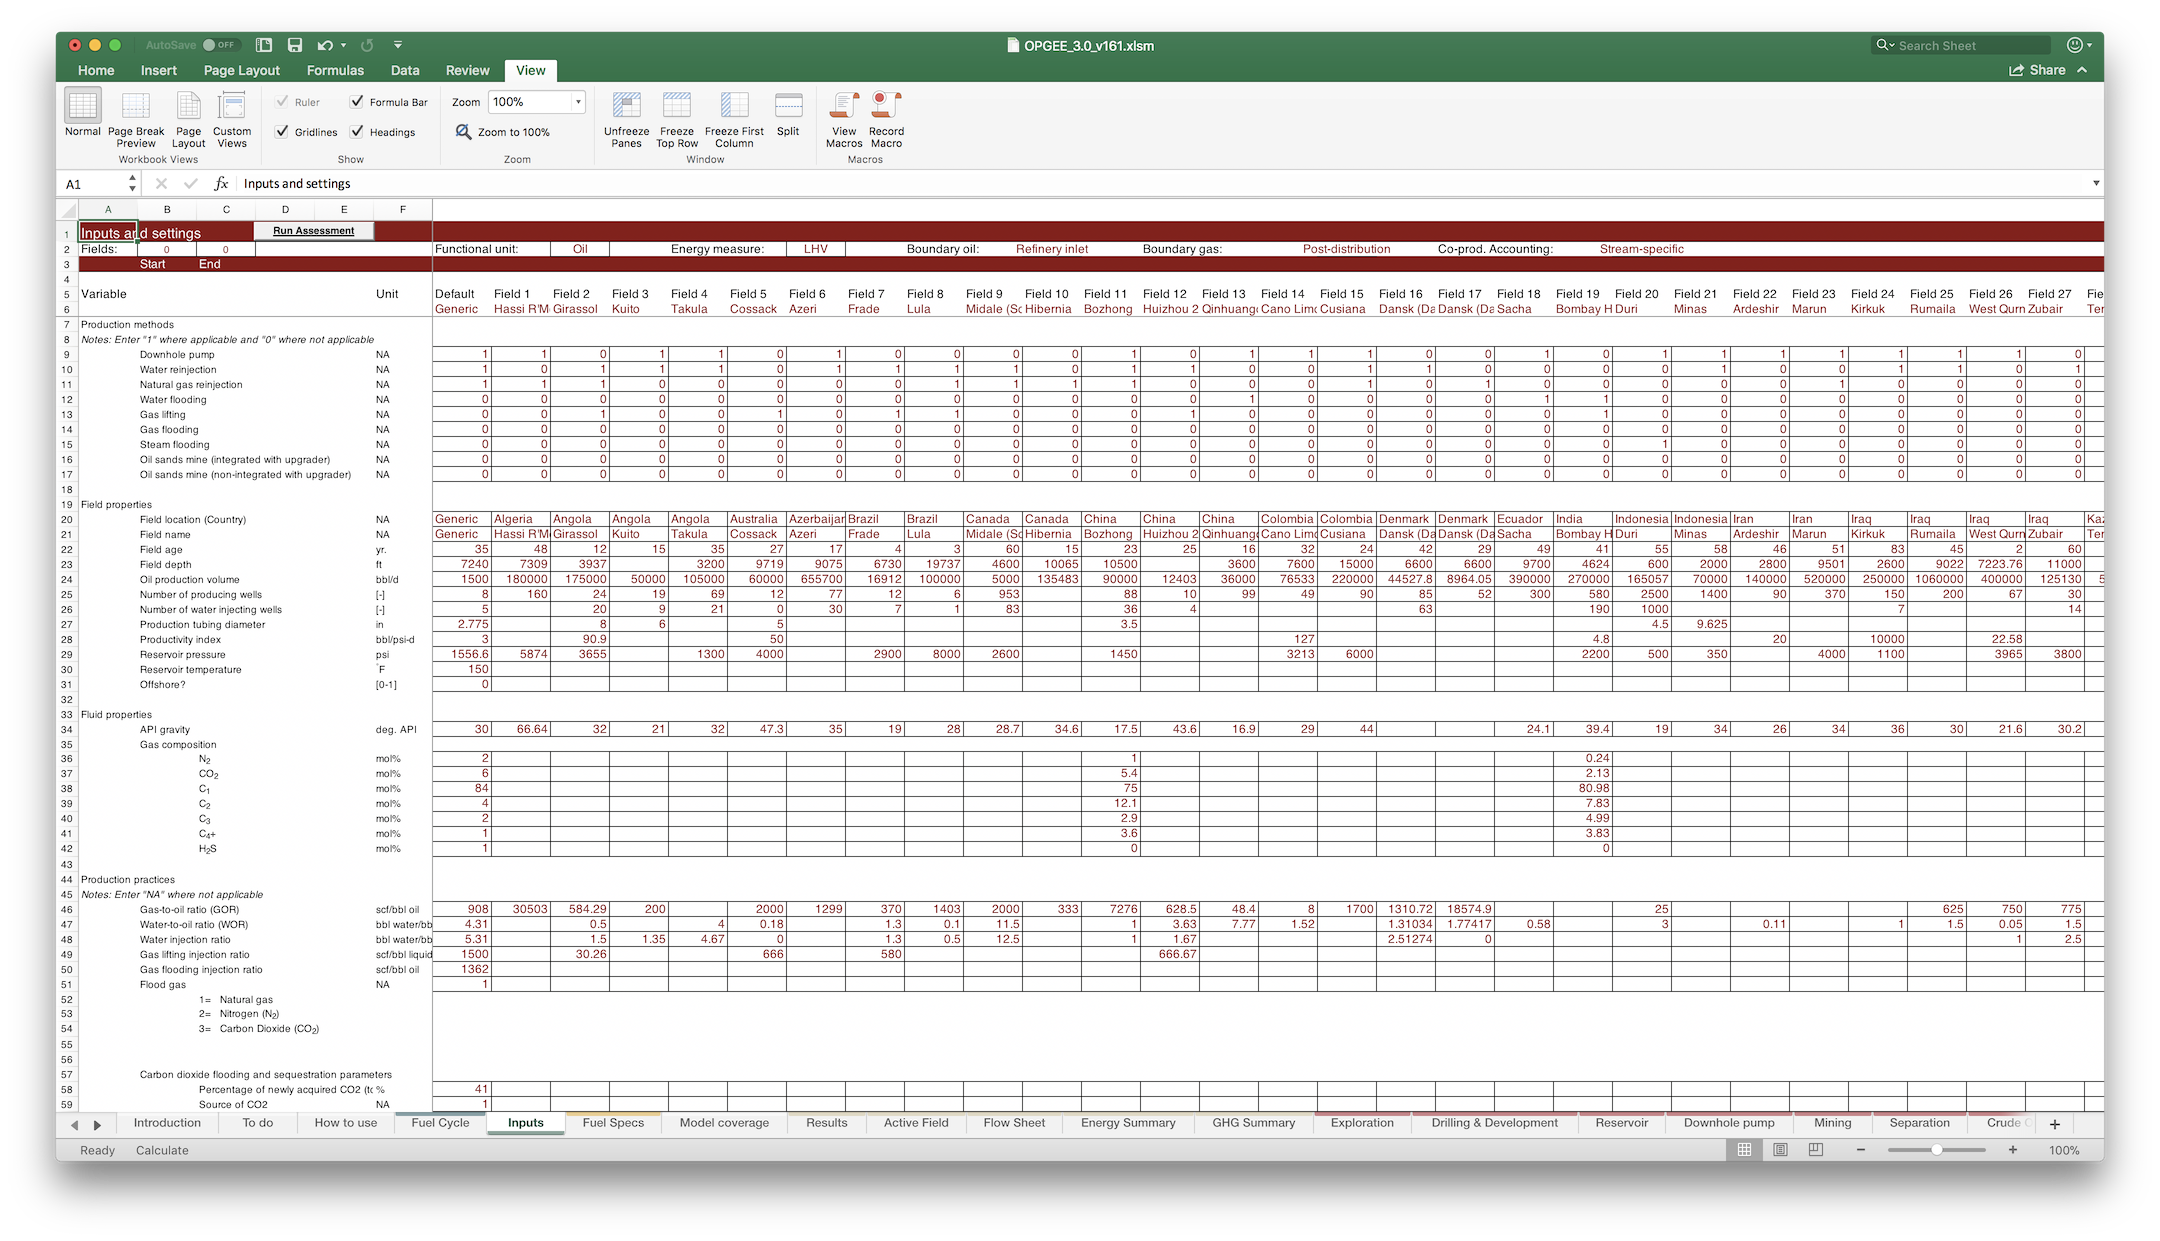
\includegraphics[width=1.2\columnwidth]{images/InputSheetSS.png}
\caption{Data input section of the \sheet{Inputs} worksheet.}
\label{fig:Inputs}
\end{figure}

OPGEE provides defaults for all required input parameters; these can be replaced with user inputs where data are available. In some cases, OPGEE calculates `smart default' values dynamically based on user inputs for other parameters. For instance, the default flaring volume is determined from NOAA data based on the specified field location \cite{Elvidge2009}. These smart defaults can also be overruled by user inputs. 

\clearpage

\subsection{Secondary interaction}
If more detailed data are available for a given oil production operation, and more specific estimates are desired, secondary interaction can be pursued by changing parameters on process-stage specific worksheets and supplementary worksheets.

It should not be necessary to change these secondary input parameters in basic use of OPGEE. The secondary parameters include parameters with less effect on the resulting emissions, that are not highly variable across operations, or that are less likely to be known by model users. Examples include compressor suction pressure and temperature, type of prime mover, or pump efficiency. Note that some of these parameters (e.g., pump efficiency) have significant effects on model results, but are not believed to be highly variable across fields. 

All secondary input parameters are free for the user to change in the input data sections of the process stage worksheets. Parameters that are classified as \emph{User Locked} (see Figure \ref{fig:Cell_types_SS} above) should not be changed because they are either calculated from other primary inputs or derived from the \sheet{Inputs} worksheet.

Figure \ref{fig:Production_Inputs} shows the input data section of the \sheet{Production \& Extraction} worksheet. Moving left to right across the screen, features of interest include:

\paragraph{Parameters and sub-parameters} In columns A through K, the names and descriptions of parameters and calculation results are numbered in a hierarchical fashion. Each parameter or calculation result has a unique number to allow ease of reference to the model. For example, the water specific gravity (2.1.2) is calculated using the concentration of dissolved solids (1.2.1.1).

\paragraph{User and default columns} Columns M and N include the user and default inputs for the production calculations. Column M is always used in the final calculations. Column N is included for reference, and includes default values. Before any user input is changed, all user values are equal to default values.

\paragraph{Free and locked cells} As shown in Figure \ref{fig:Cell_types_SS} above, \emph{User Free} and \emph{Default Free} cells are included with light tones, while \emph{User Locked} and \emph{Default Locked} cells are included with dark tones. For example, in Figure \ref{fig:Production_Inputs} the highlighted cell M37 represents the mol\% of methane (C$_1$) in the associated gas. Because this quantity is a key input parameter and is defined on the \sheet{Inputs} worksheet, it is marked here as \emph{User Locked}. Therefore, if the user wishes to change the gas composition, this should be done on the \sheet{Inputs} worksheet where gas composition is classified as \emph{User Free}.

\paragraph{Units} In column O, units are listed for all input parameters, variables, and calculation results (where applicable).

\paragraph{User and default reference} Columns Q and S are spaces to record the data sources of input parameters. Where applicable, the source of the default value is listed in the \emph{Default reference} column. If a user changes a parameter to a non-default value, they can place any desired information about the source (such as author, page, dataset, vintage, data quality, expected uncertainty, etc.) in the \emph{User reference} column.

\paragraph{Notes} To the right of the default reference column is the notes column (not shown, column Y). The \emph{Notes} column contains explanatory notes or other information that may be useful to the user.

\begin{figure}[t]
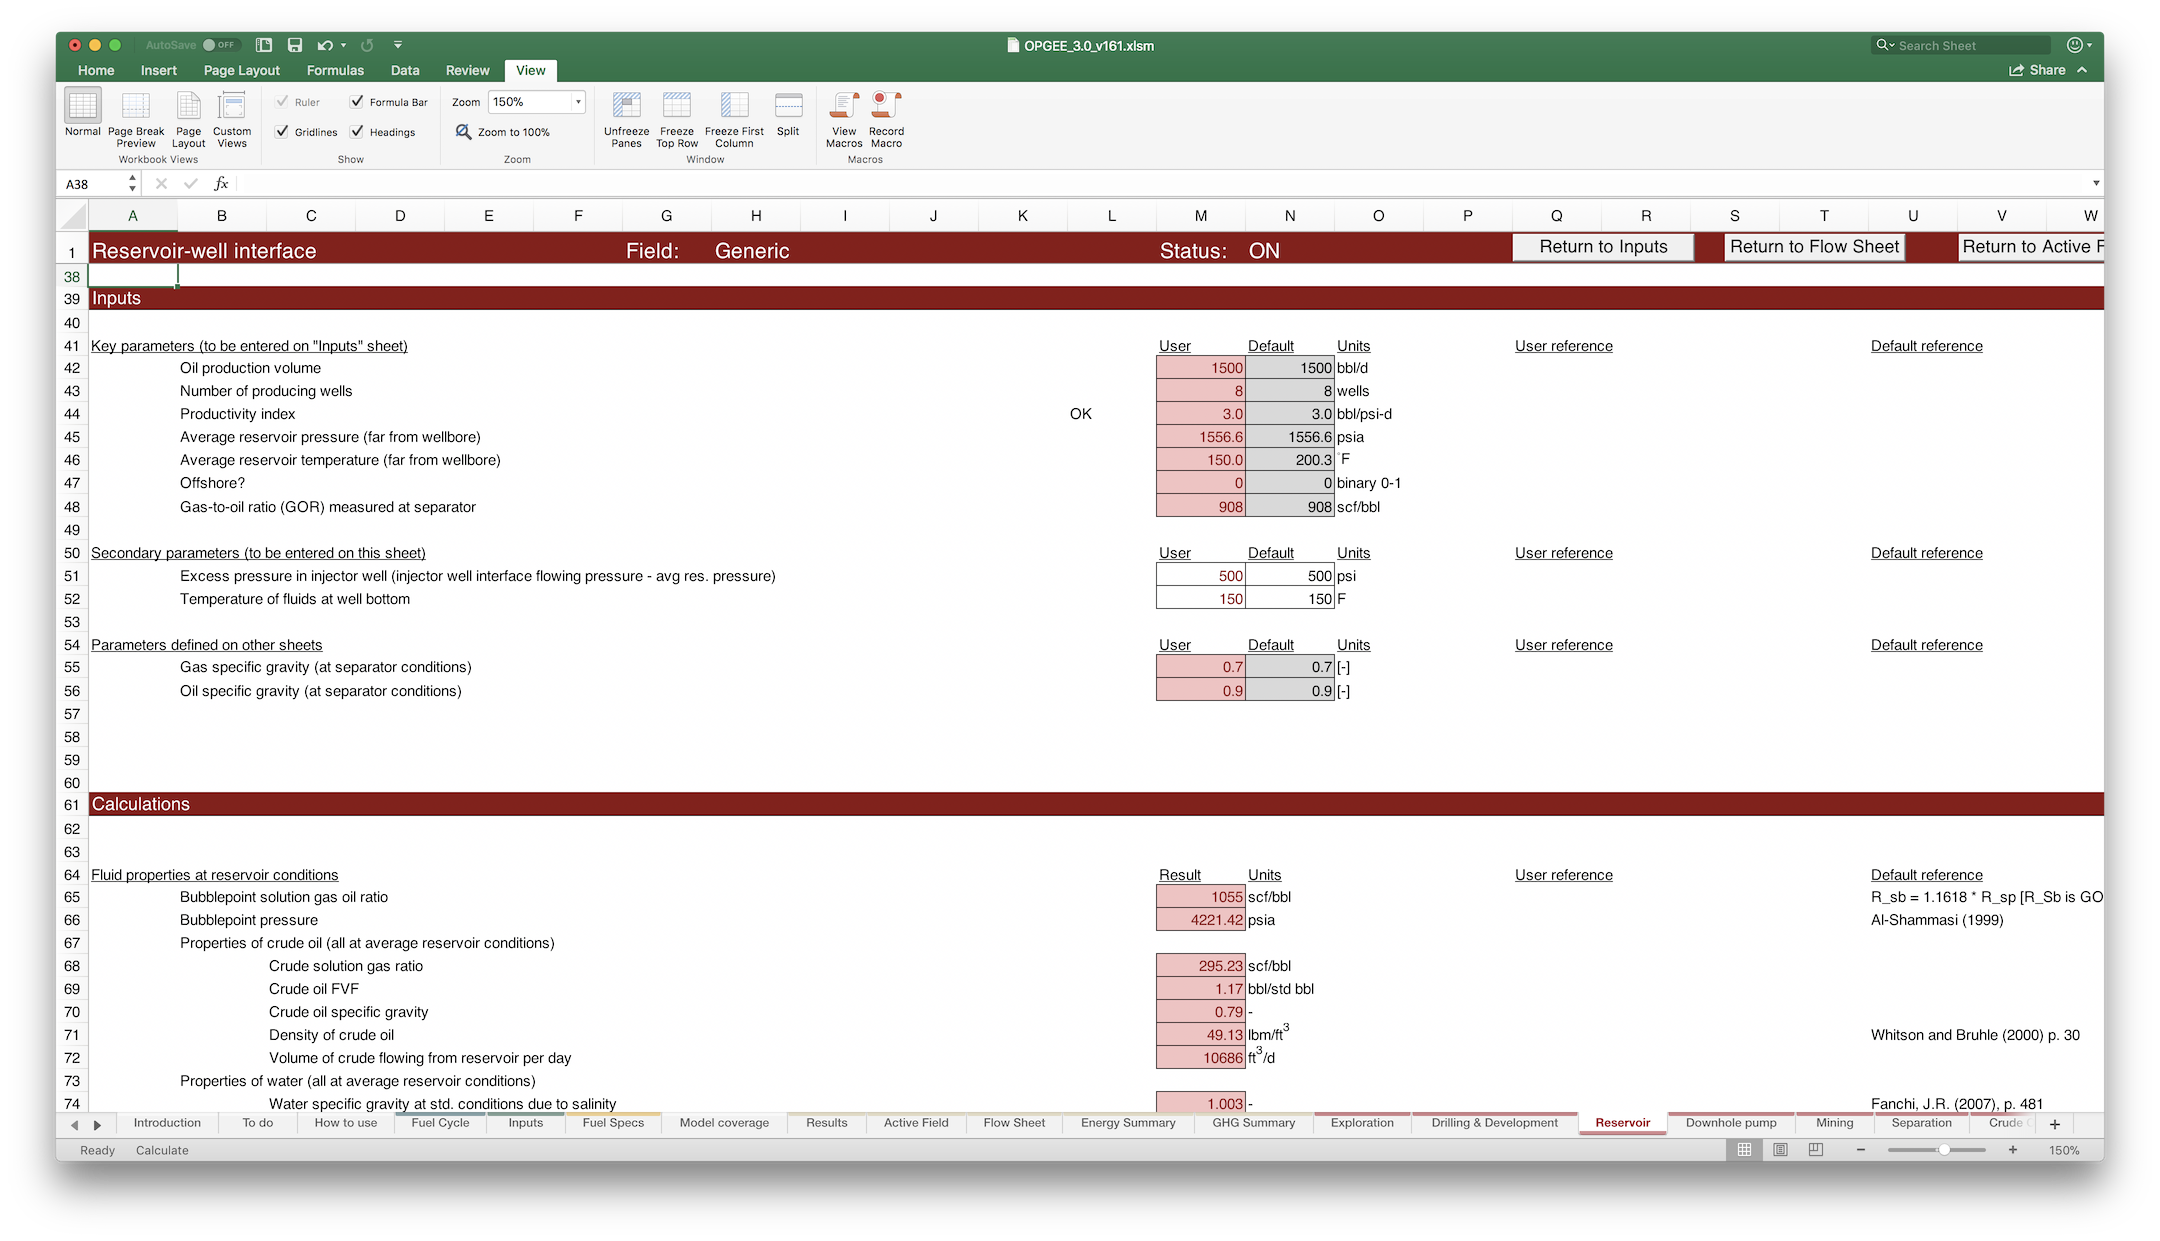
\includegraphics[width=1.2\columnwidth]{images/InputSS.png}
\caption{Input data section of \sheet{Reservoir} worksheet. User inputs are in column M, while defaults are kept as reference in column N.}
\label{fig:Production_Inputs}
\end{figure}

\subsection{Checking for errors}
It is possible to mistakenly enter data that are invalid, contradictory, or otherwise result in errors. 

A summary indicator for model errors appears in the \sheet{Results} worksheet as the "Overall Check." \marginnote{Results 2.14} An overall check error is the result of an error in any of the fields that included in the model run, which appears as an error in the "Field by Field Check." \marginnote{Results 2.13} To investigate an error in a specific field, the "End field" should be set equal to the field number of the field in question and the "Run Assessment" button should be clicked again. This will populate the \sheet{Active Field} worksheet with the calculations regarding the error-causing field. Here, the error can be traced to a particular worksheet and cell by examining the 'Specific error checks.' \marginnote{Active Field 4.1.1 - 7.1.29} Specific error checks can be debugged by moving to the worksheet and cell in question and tracing any logical or inputs errors that have flagged that error check. Common sources of errors include logical errors in pathway selection (e.g., more than one mutually exclusive technology selected) and input errors (e.g., gas composition sums to more than 100 mol\%).

Hints for using OPGEE without errors are given in Box 2.2.

\begin{figure}
\fcolorbox{black}{gray!20}{ 
\parbox{\tw}{\boxtitle{Box 2.2: Hints for using OPGEE without errors}
\begin{small}
\begin{enumerate}
\item Do not change formulas in \emph{User locked} or \emph{Default locked} cells, as these can result in mis-calculation;
\item Always check error reports in \sheet{Results} section 2.14 and, if necessary, section 2.13, for errors before considering results final;
\item Use care to collect physically realistic and consistent data where default values will be overwritten (e.g., if depth of field is greatly increased, operating pressure will often increase as well);
\item To ensure reproducibility of results, document any sources for user inputs in the `User Reference' column;
\item Save individual field assessments as separate worksheets to prevent incorrect propagation of changed cells.
\end{enumerate}
\end{small}
}} 
\end{figure}




\clearpage

\subsection{Results}

After the user enters data to the \sheet{Inputs} sheet and clicks the Run Assessment button, OPGEE computes the resulting GHG emissions. The results are for the last field (End field) analyzed are stored in the \sheet{Active Field} sheet, \marginnote{Active Field Table 1.1} while the results from all fields are stored in the \sheet{Results} in tabular form \marginnote{Results 2.1 - 2.14} in gCO$_2$ equivalent GHG emissions per MJ LHV crude oil delivered to the refinery gate.\footnote{The heating value basis of the denominator crude oil can be changed so that emissions are calculated per MJ HHV of refinery input. This can be changed on the \sheet{Fuel Specs} worksheet. See discussion below in Section \ref{sec:properties_fuels}.} Emissions are broken down by stage (generally) or by type, with fugitive emissions for all process stages summed together for convenient interpretation as `VFF' \marginnote{Active Field Fig. 1.1} emissions. Total energy consumed per unit of energy delivered to the refinery gate is also presented in tabular and graphical form. \marginnote{Active Field Table 1.2, Figure 1.2} These tabular and graphical results are illustrated in Figures \ref{fig:Results_example}.

\begin{figure}[t]
\includegraphics[width=1.2\columnwidth]{images/Results_Example.png}
\caption{Graphical results for an example crude oil. These results from \sheet{Active Field} Tables 1.1 and 1.2, Figures 1.1 and 1.2.}
\label{fig:Results_example}
\end{figure}


\clearpage




%%%%%%%%%%%%%%%%%%%%%%%%%%%%%%%%%%%%%
\section{Inputs} \label{sec:inputs}

\subsection{Further details regarding the Inputs sheet}
OPGEE has a built-in capability to analyze a number of fields or oil production projects and bookkeep the results for comparison and further analysis.

The capability to analyze multiple fields simultaneously is provided by a Microsoft VBA macro. In addition to running a number of fields in sequence, the macro programmatically resolves significant errors that arise from input data inconsistencies. It also automates iterative calculations such as the reconfiguration of gas composition in the case of gas lift or setting gas export to zero by incrementally increasing gas reinjection.

At the top of the \sheet{Inputs} worksheet the user enters the fields to be assessed by entering the starting field and the ending field. In the input data section\marginnote{Inputs 1.1-1.8} the user enters available data for each assessed field. When limited datasets are available, the assessment macro will complete the datasets by filling required inputs with defaults and smart defaults where applicable. The results are generated for all fields in one computational run. The macro is started by pressing the ``Run Assessment'' command button.


\subsection{Assessment macro description}
\begin{figure}[t]
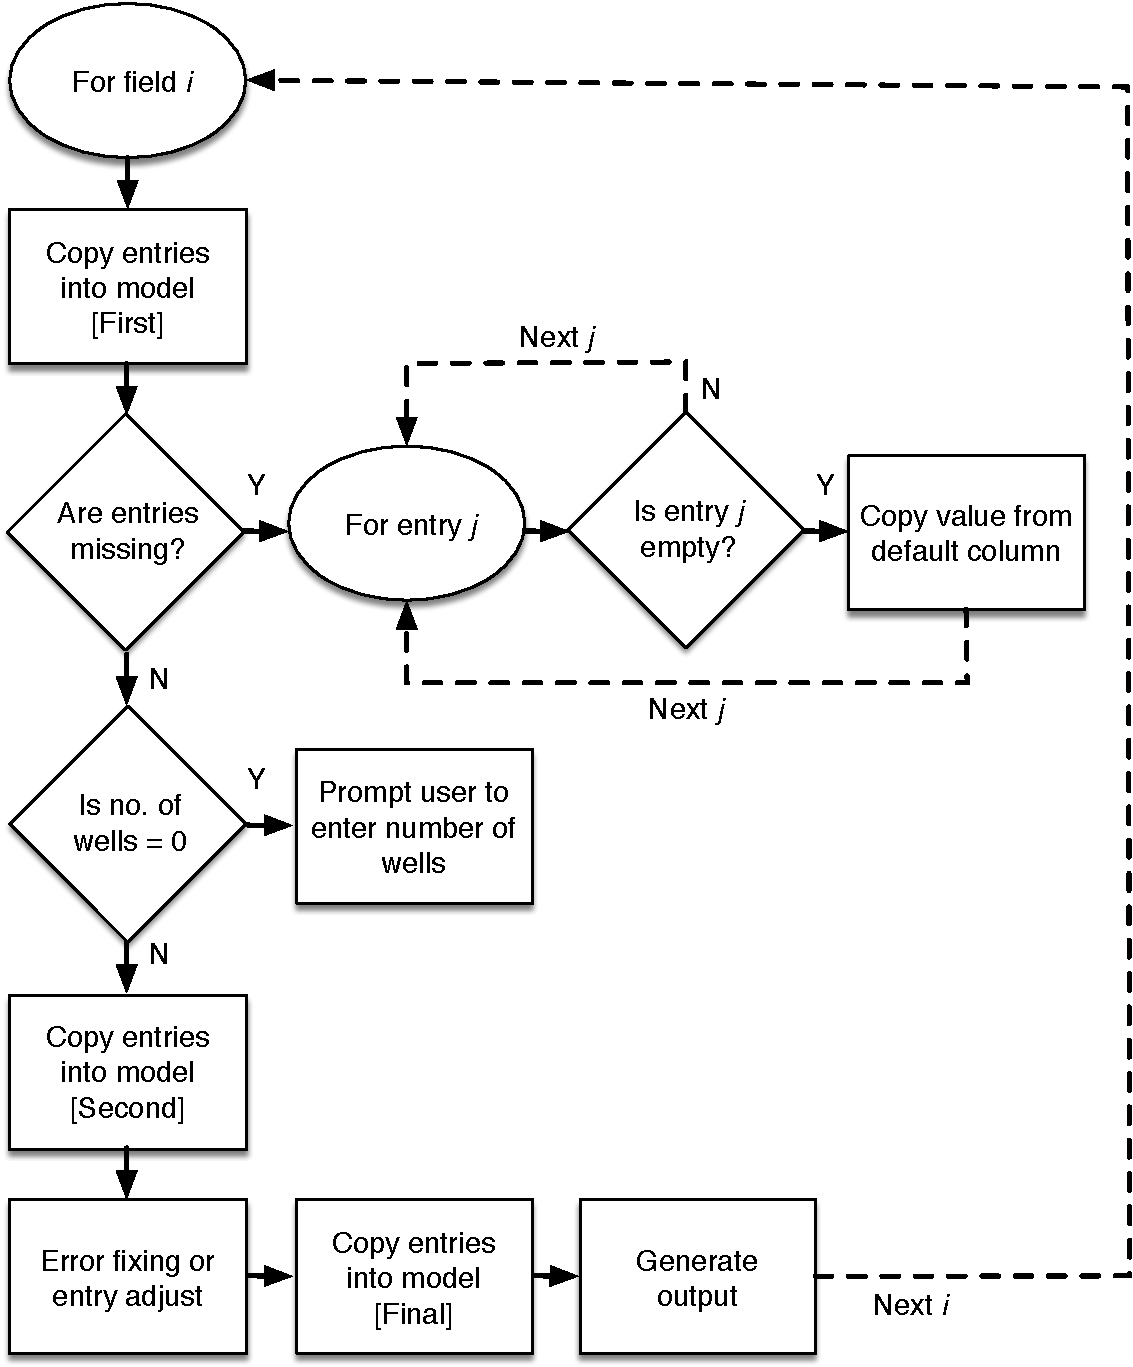
\includegraphics[width=0.75\columnwidth]{images/MacroLogic1.pdf}
\caption{Logical structure of the assessment macro.}
\label{fig:macro_logic_1}
\end{figure}

Figure\,\ref{fig:macro_logic_1} shows the outer structure of the assessment macro. For every field under study, the macro first copies user entries into the (\sheet{Active Field}) worksheet. It then checks for empty user entries. For every empty user input, the macro copies the default value from the (\sheet{Active Field}) worksheet. In the case of "0" entry for the number of producing wells, a warning appears and prompts the user to enter a valid number of producing wells. When the data set of the field under study is complete, the macro copies the complete set of data into the (\sheet{Active Field}) worksheet, initiates the error correction and entry adjustments procedure, and returns the completed and corrected/adjusted set of data into the (\sheet{Results}) worksheet. Finally the macro copies the full data set back into the (\sheet{Active Field}) worksheet and returns the results into the (\sheet{Results}) worksheet. The same process is repeated for each field under study.

The assessment macro is capable of fixing errors, performing iterative calculations and adjusting input parameters where necessary. It is not practical to perform these computational tasks manually when assessing a large number of projects (100+). The macro ensures consistent treatment across all fields. Errors that are addressed in the macro include:
\begin{itemize}
\item Discrepancies between country-average default flaring rate and entered GOR (e.g., flaring module predicts more flaring than field has gas available);
\item Discrepancies between default fugitive emissions of gaseous components and gas available from production;
\item Requirement to iteratively solve for the gas composition in the wellbore in the case of gas lift;
\item Error with productivity index resulting in negative bottomhole pressures;
\item Error resulting from very large frictional lifting penalties due to too-small default wellbore diameter;
\item Requirement to iteratively solve for gas reinjected to result in 0 gas export.
\end{itemize}
Appendix \ref{sec:macro_error} details the functioning of these error correction features.






%%%%%%%%%%%%%%%%%%%%%%%%%%%%%%%%%%%%%%%%%%%%%
%%%%%%%%%%%%%%%%%%%%%%%%%%%%%%%%%%%%%%%%%%%%%
%%%%%%%%%%%%%%%%%%%%%%%%%%%%%%%%%%%%%%%%%%%%%

\part{Technical documentation}

%%%%%%%%%%%%%%%%%%%%%%%%%%%%%%%%%%%%%%%%%%%%%
%%%%%%%%%%%%%%%%%%%%%%%%%%%%%%%%%%%%%%%%%%%%%
%%%%%%%%%%%%%%%%%%%%%%%%%%%%%%%%%%%%%%%%%%%%%





%%%%%%%%%%%%%%%%%%%%%%%%%%%%%%%%%%%%%%%%%%%%%
%%%%%%%%%%%%%%%%%%%%%%%%%%%%%%%%%%%%%%%%%%%%%
%%%%%%%%%%%%%%%%%%%%%%%%%%%%%%%%%%%%%%%%%%%%%

\chapter{\sheet{Active Field} gathering worksheet}
\label{sec:active_field}


\clearpage

%%%%%%%%%%%%%%%%%%%%%%%%%%%%%%%%%%%%%
\section{Introduction to the \sheet{Active Field} worksheet}



\clearpage

%%%%%%%%%%%%%%%%%%%%%%%%%%%%%%%%%%%%%
\section{GHG calculations on the \sheet{Active Field} worksheet}
In this worksheet the total energy consumption and GHG emissions for the most recently processed field are calculated and displayed in graphical form. Both the total energy consumption and total GHG emissions are calculated by process stage (e.g., Production \& Extraction). First the total energy consumption is calculated as: \marginnote{Active Field 3.1.1. - 3.7.1, Table 1}
%%%%%%%%%%%%%
\begin{equation} 
E_{tot} = \frac{E_{tot,dir} + E_{tot,ind} + EL_{VFF}}{E_{tot,out}} \quad\quad\footnotesize{\text{[MJ/MJ$_{out}$]}}
\end{equation}
%%%%%%%%%%%%%
where $E_{tot}$ = total energy consumption of the process [MJ/MJ$_{out}$]; $E_{tot,dir}$ = total direct energy consumption (calculated in the \sheet{Energy Consumption} worksheet as net energy consumption) [MMBtu/d]; $E_{tot,ind}$ = total indirect energy consumption (calculated in the \sheet{Energy Consumption} worksheet) [MMBtu/d]; $EL_{VFF}$ = total energy loss from VFF emissions [MMBtu/d]; and $E_{tot,out}$ = total process energy output [MMBtu/d]. The total process energy output is calculated as: \marginnote{Active Field 5.1.1. - 5.9.1}
%%%%%%%%%%%%%
\begin{equation}\label{eq:tot_process_output}
E_{tot,out} = Q_{o}\,\text{HV}_{o} + E_{ngl,blend} - E_{co,net} \quad\quad\footnotesize{\text{[MMBtu/d]}}
\end{equation}
%%%%%%%%%%%%%
where $E_{tot,out}$ = total process energy output [MMBtu/d]; $Q_{o}$ = volume of oil production [bbl/d]; HV$_{o}$ = heating value of crude oil [MMBtu/bbl]; \newline $E_{ngl,blend}$ = amount of produced NGL that is added to crude oil [MMBtu/d]; and $E_{co,net}$ = net crude oil consumption, if applicable [MMBtu/d]. The heating value HV for the denominator crude oil can be selected as LHV or HHV. \marginnote{Fuel Specs 1.1}\\
If the allocation of co-products is done by energy value and not displacement then eq.\,\eqref{eq:tot_process_output} becomes:
%%%%%%%%%%%%%%%%%%%
\begin{equation} 
E_{tot,out} = Q_{o}\,\text{HV}_{o} + E_{ngl,blend} - E_{co,net} + |\sum_k E_{k,exp}| \quad\text{and}\,\, E_{k,exp}< 0 
\end{equation}
%%%%%%%%%%%%%%%%%%
where $|\sum_k E_{k,exp}|$ = absolute sum of all energy exports [MMBtu/d].

Total energy consumption is allocated by process stage using the fraction of direct energy consumed in a stage (not including the energy consumption of electricity generation). The allocation of energy consumption to different process stages has no effect on the total energy consumption.

For each process stage, GHG emissions are broken down into three categories: (i) combustion/land use, (ii) VFF, and (iii) credit/debt. For combustion/land use emissions, the direct GHG emissions and land use GHG emissions associated with the process stage are summed \marginnote{GHG \\ Emissions Table 1} in the \sheet{GHG emissions} worksheet. The direct GHG emissions from electricity generation, if any, are divided between the production \& extraction and surface processing stages based on the shares of total direct energy consumption between these stages. 

VFF emissions associated with a process stage are summed from the \sheet{GHG emissions} \marginnote{GHG \\ Emissions Table 1} worksheet. Indirect GHG emissions calculated in the \sheet{GHG emissions} worksheet represent the total net credit/debt, which is \marginnote{GHG \\ Emissions Table 2} allocated by process stage using the same allocation method used for allocating the total energy consumption.

This sheet also includes CO$_2$ sequestration credited accruing to the oilfield, which are described in Section \ref{sec:Sequestration}.

Finally, the total energy consumption and GHG emissions from the process stages of crude oil extraction and surface processing of associated fluids are integrated with the total energy consumption and GHG emissions of crude oil transport to the refinery to calculate the life cycle energy consumption and GHG emissions on a well-to-refinery basis. The life cycle GHG emissions, for example, are calculated as:
\begin{equation}
EM_{LC} = EM_{PP,tot}\,\epsilon_{CT}+EM_{CT,tot} \quad\quad\footnotesize{\left[\frac{\text{gCO$_{2}$eq}}{\text{MJ$_{ref}$}}\right]}
\end{equation}
where $EM_{LC}$ = life cycle GHG emissions [gCO$_{2}$eq/MJ$_{F}$]; $EM_{PP,tot}$ = total GHG emissions from the process stages of crude oil production and processing [gCO$_{2}$eq/MJ$_{out}$]; $\epsilon_{CT}$ = crude oil transport loss factor (calculated based on the amount of crude oil lost in transportation) [-]; and $EM_{CT,tot}$ = total GHG emissions from transport [gCO$_{2}$eq/MJ$_{ref}$]. 1 MJ$_{out}$ is one MJ of energy output from crude oil production and processing; and 1 MJ$_{ref}$ is one MJ at refinery gate. 

The life cycle energy consumption and \marginnote{Active Field \\ Tables 1.1 - 1.2 \\ Figures 1.1 - 1.2 } GHG emissions are shown in tabular and graphical formats with full GHG emissions breakdown. The total GHG emissions has a separate category for VFF emissions. The energy content of fuels lost to VFF emissions is not tracked as a separate category of energy consumption. 


\clearpage

%%%%%%%%%%%%%%%%%%%%%%%%%%%%%%%%%%%%%
\section{Smart defaults and uncertainty distributions for missing key parameters}
\label{sec:smart_defaults}


\subsubsection{Default field age}

Field age data were collected for global oil fields. A total of 6,502 global oil fields were collected from the Oil \& Gas Journal \emph{2010 Worldwide Oil Field Production Survey} \cite{OGJ2009a}. A total of 4837 of these fields had reported discovery dates. No data are available on date of first production, although this will most commonly occurs less than 5 years after discovery.

The histogram of field discovery dates is shown in Figure \ref{fig:age_distribution_all}. Because the dataset has poor coverage of field-specific production data, a production-weighted average age figure was not thought to provide an accurate representation of the true production-weighted age distribution, so this was not calculated. The mean date of discovery in the dataset was 1972.1. \marginnote{Active Field 2.2.3} If a conservative 3 year development timeline is assumed, an average of 35 years has elapsed between 1975 and 2010.

However, many of these fields are likely small fields that do not supply large quantities of oil to the global export markets. It is known that giant oilfields are somewhat older on average than the general field population \cite{Simmons2005, Simmons2006, Deffeyes2001, Deffeyes2005}. A database of 116 giant oilfields was collected (defined as all producing over 100 kbbl/d in the year 2000) \cite[Appendix A]{Simmons2006}. In total, these 116 fields produced $\approx$32,000 kbbl/d, or some 43\% of global oil production in 2000.

These giant fields have a count distribution and production-weighted average age distribution that are somewhat older than the complete set of global fields. Figure \ref{fig:age_distribution_giant} shows these distributions. The production-weighted average discovery year of the sample was 1960.2, for an average age of 40 years since discovery at the time of production data collection (weighted by year 2000 production data). Data on giant oilfield production in 2010 are not available. Due to the general global slowdown in the discovery of giant fields since the 1970s, it is likely that the age distribution of giant oilfields has not shifted in step with advancing years. Therefore, the production-weighted average age for large fields is likely now greater than 40 years.

\begin{figure}[t]
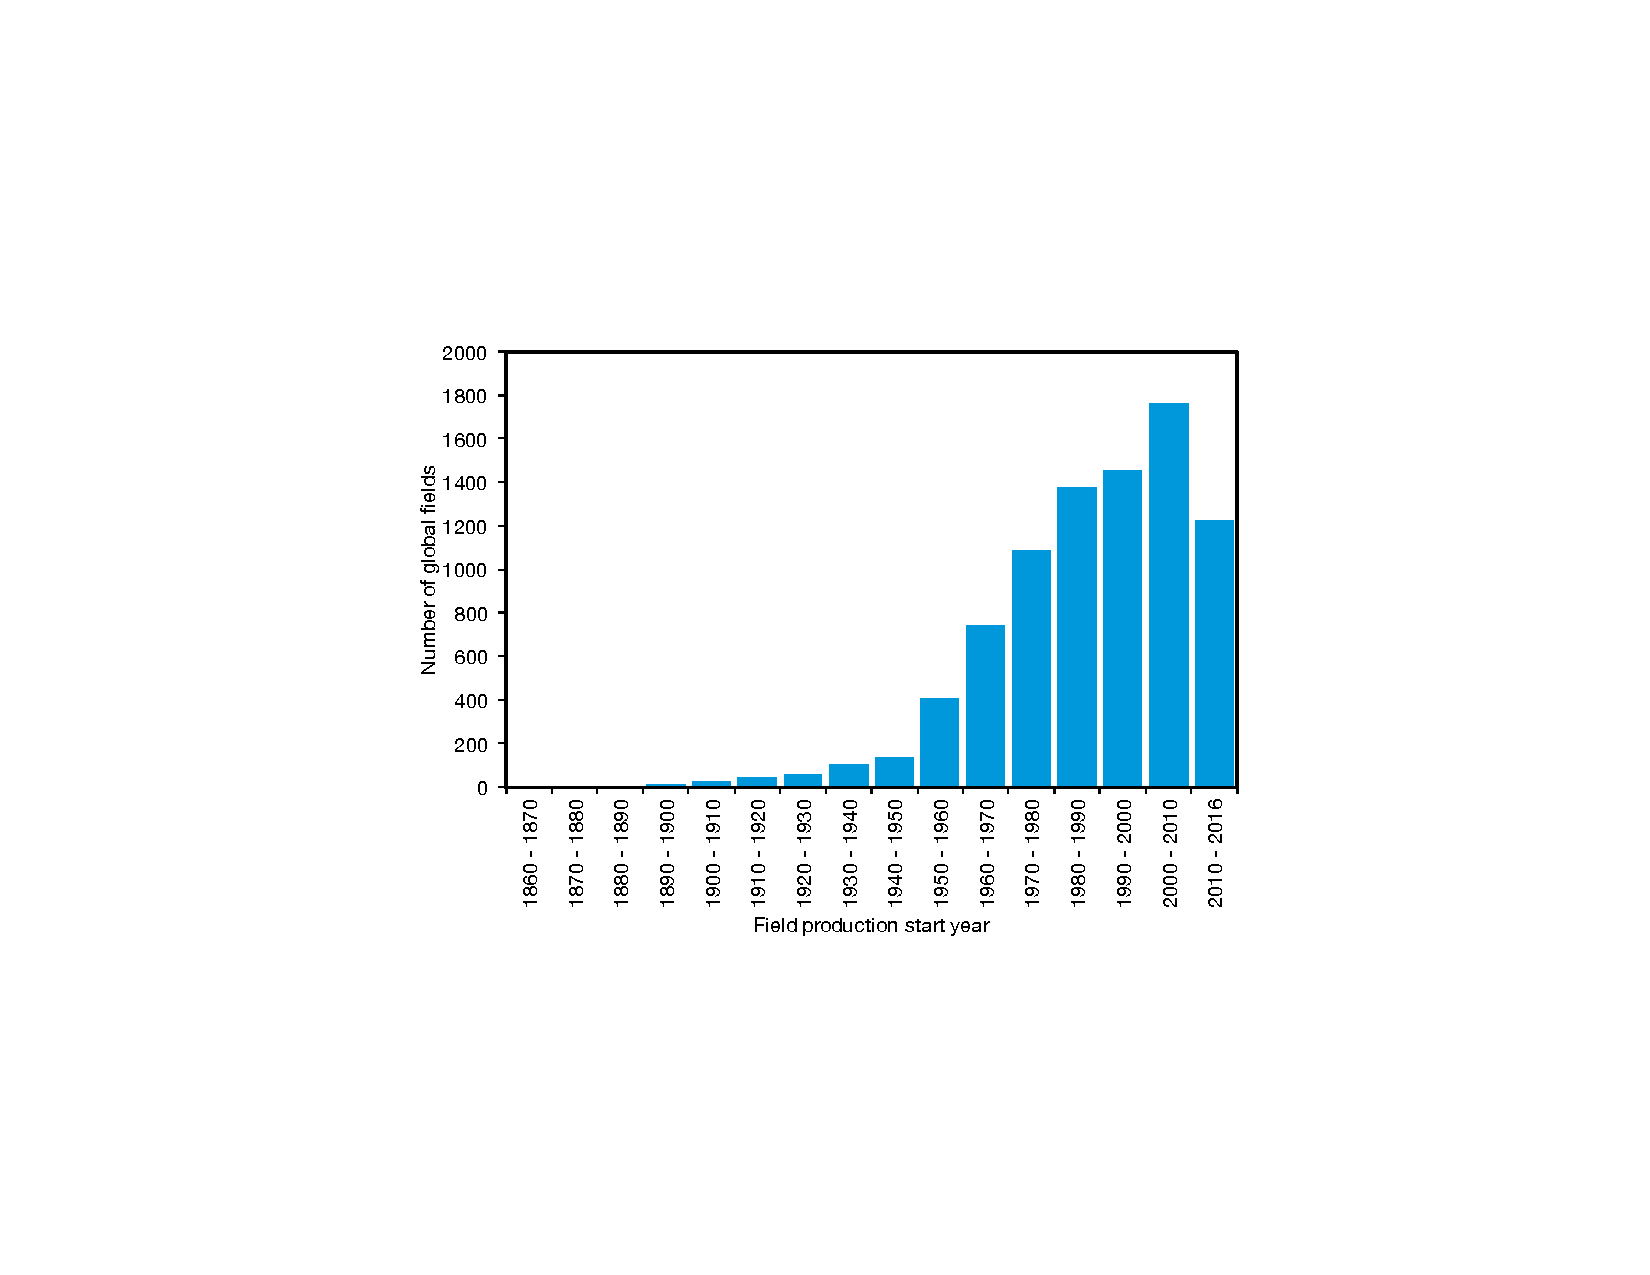
\includegraphics[width=0.85\columnwidth]{images/age_distribution_all.pdf}
\caption{Distributions of global oilfield ages. Mean date of discovery (by count not by production-weighted average) is 1978.4.}
\label{fig:age_distribution_all}
\end{figure}

\begin{figure}[t]
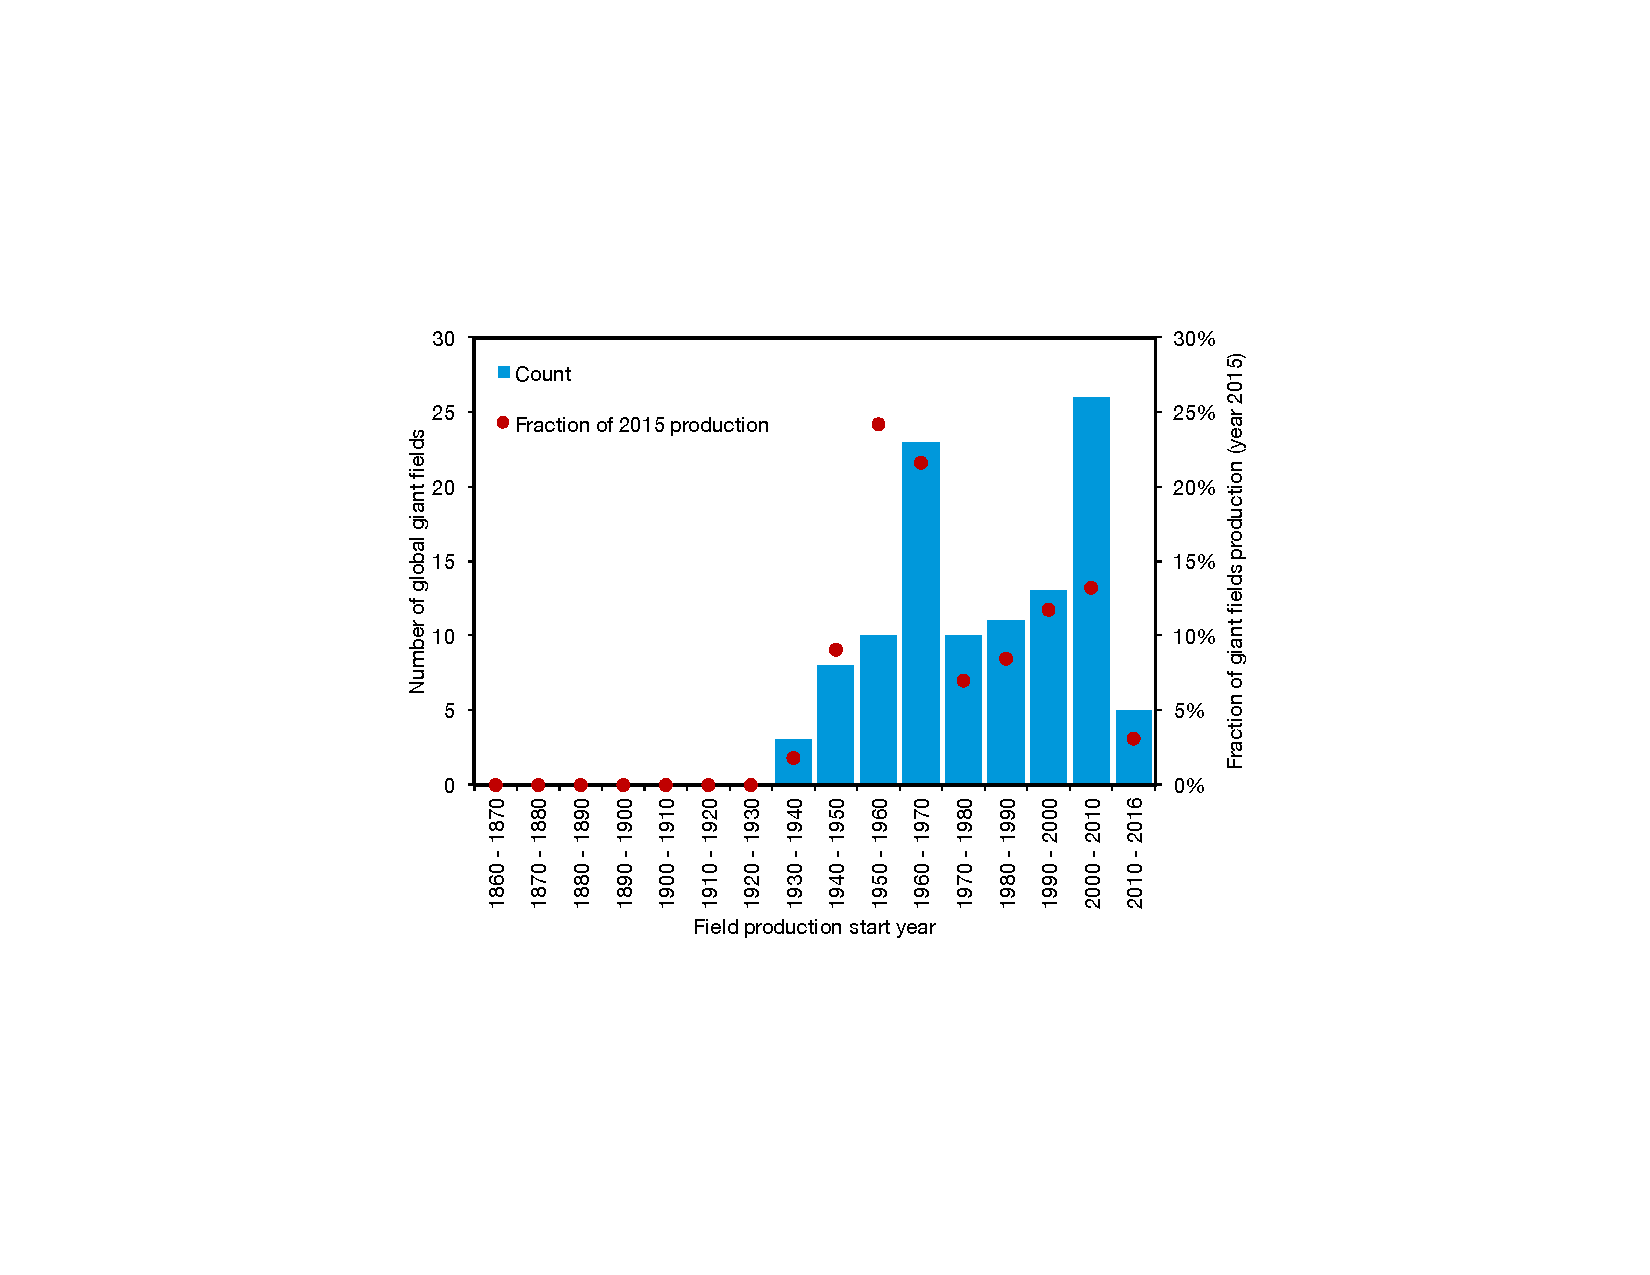
\includegraphics[width=0.85\columnwidth]{images/age_distribution_giant.pdf}
\caption{Distributions of giant oilfield ages. Mean date of discovery (by production-weighted average) is 1960.2.}
\label{fig:age_distribution_giant}
\end{figure}






\subsubsection{Default field depth}

Field depth data were collected for a large number of global oil fields \cite{OGJ2009a}. A total of 6,502 global oil fields were collected from the Oil \& Gas Journal \emph{2010 Worldwide Oil Field Production Survey}. Of these fields, 4,489 fields had depth data presented. For fields where a range of depths was presented, the deeper depth is used.

The distribution of depths by number of fields per depth range is presented in Figure \ref{fig:depth_distribution}. Because of sporadic reporting of production data in the same dataset, a production-weighted depth figure was not thought to provide an accurate representation. \marginnote{Active Field 2.2.4}The mean depth for these 4,489 fields is 7,238, or $\approx$ 7,240 ft. The standard deviation is 3,591 ft. The depth distribution has a longer right (deep) tail than left (shallow) tail, so the mean is somewhat larger than the median (median = 6,807 ft).

\begin{figure}[t]
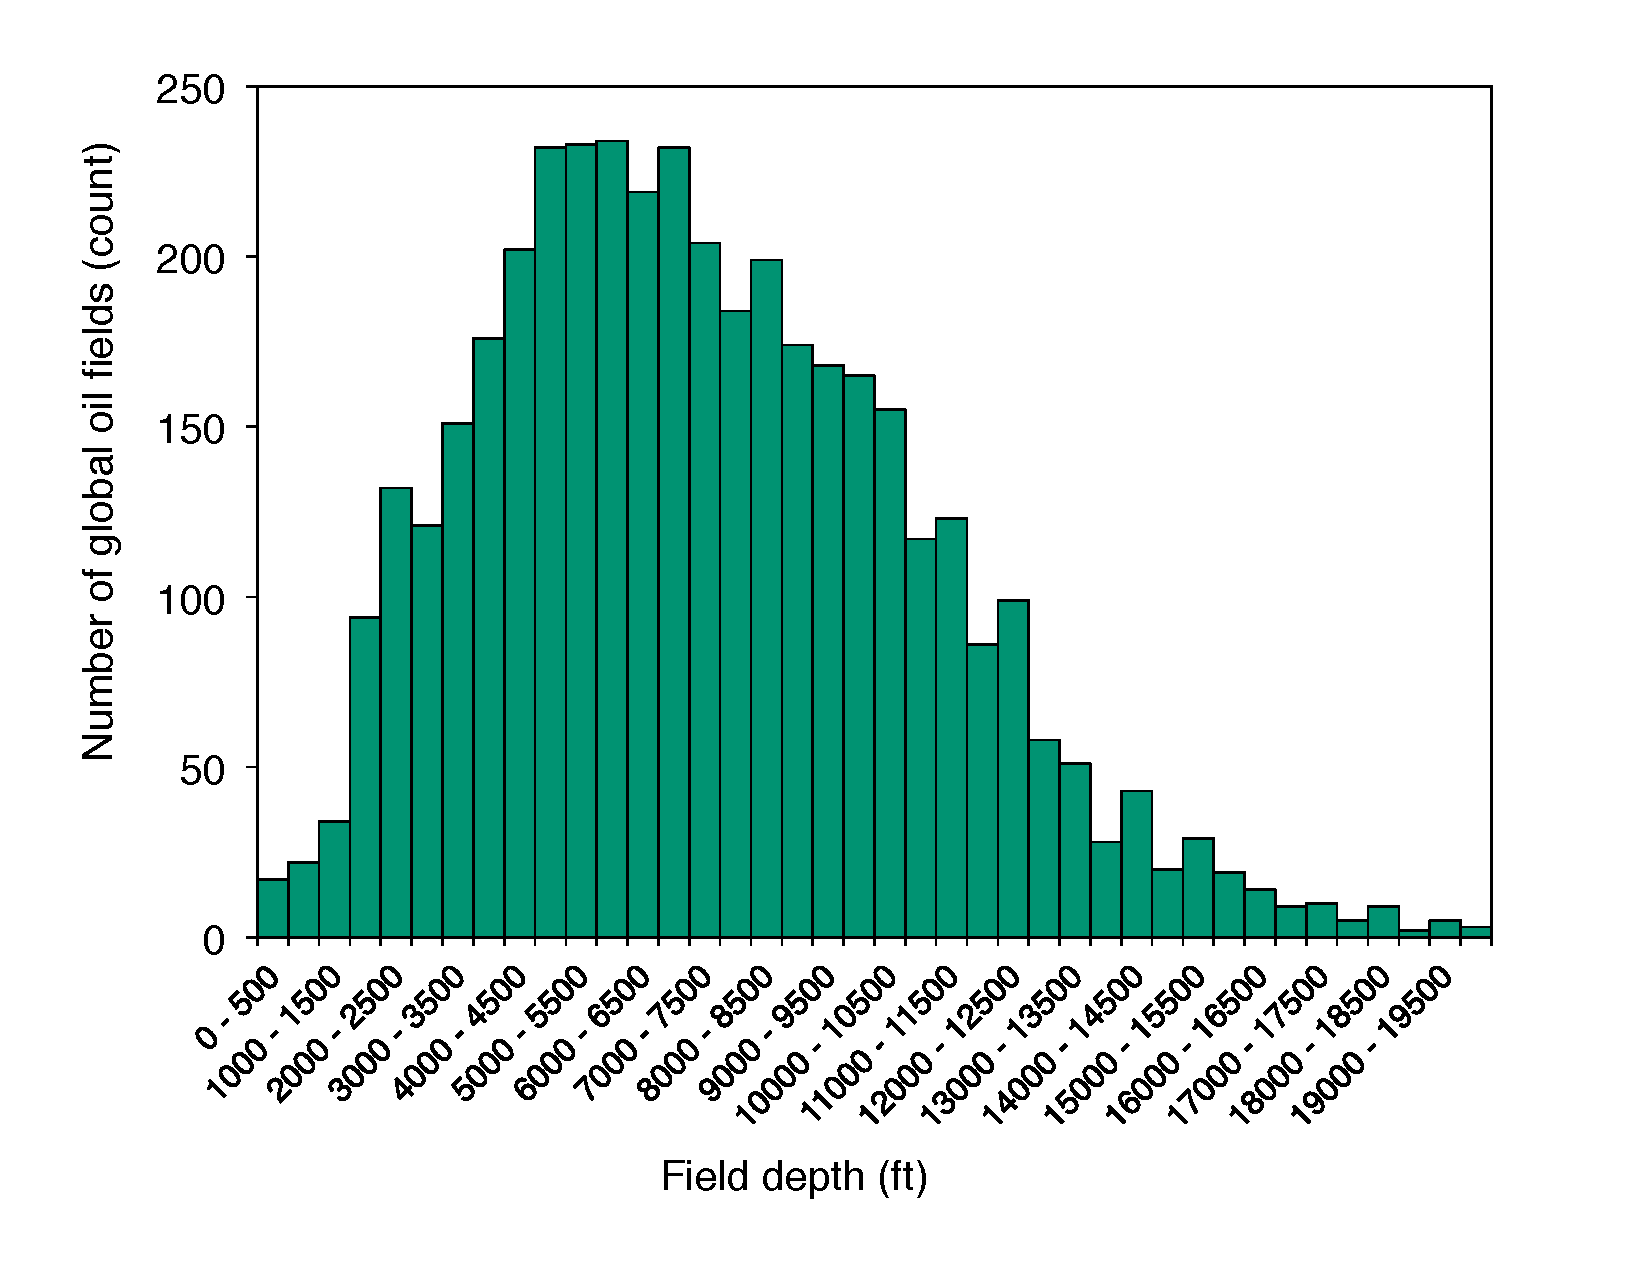
\includegraphics[width=0.8\columnwidth]{images/depth_distribution.pdf}
\caption{Distributions of global oilfield depths in bins of 500 ft depth. $N$ = 4489 fields, mean = 7238 ft, SD = 3591 ft, median = 6807 ft.}
\label{fig:depth_distribution}
\end{figure}



\subsubsection{Default production per well} \label{sec:well_production}

Country-level oil production data and numbers of producing wells were collected for a large number of oil producing countries. Data from a total of 107 oil producing countries were collected from the Oil \& Gas Journal \emph{2010 Worldwide Oil Field Production Survey} \cite{OGJ2009b}. Production data and operating well counts for 2008 were collected from 92 of these 107 countries. 

The distribution of per-well productivities for all countries is shown in Figure \ref{fig:productivity_distribution_all}. A majority of oil producing countries produced less than 500 bbl/well-d. Weighting these well productivities by country-level share of global production, we see a very similar distribution.

Because of the large number of countries producing less than 500 bbl/well-d, we plot the distribution for countries under 500 bbl/well-d (see Figure \ref{fig:productivity_distribution_low}). For the 55 countries with per-well productivity less than 500 bbl/well-d, the most common productivity by number of countries was the 0-25 bbl/well-d. However, when weighted by total production, the most common productivity bin is 75-100 bbl/well-d. 

In 2008, the world produced 72822 kbbl/d from 883691 wells, for an average per-well productivity of 82 bbl/well. \marginnote{Active Field 2.2.6} However, the very low productivity of the US oil industry (representing $\approx$512000 wells) pulls down this average significantly. Non-US producers averaged a per-well productivity of 183 bbl/well-d, which is used as default well productivity in OPGEE.

\begin{figure}[t]
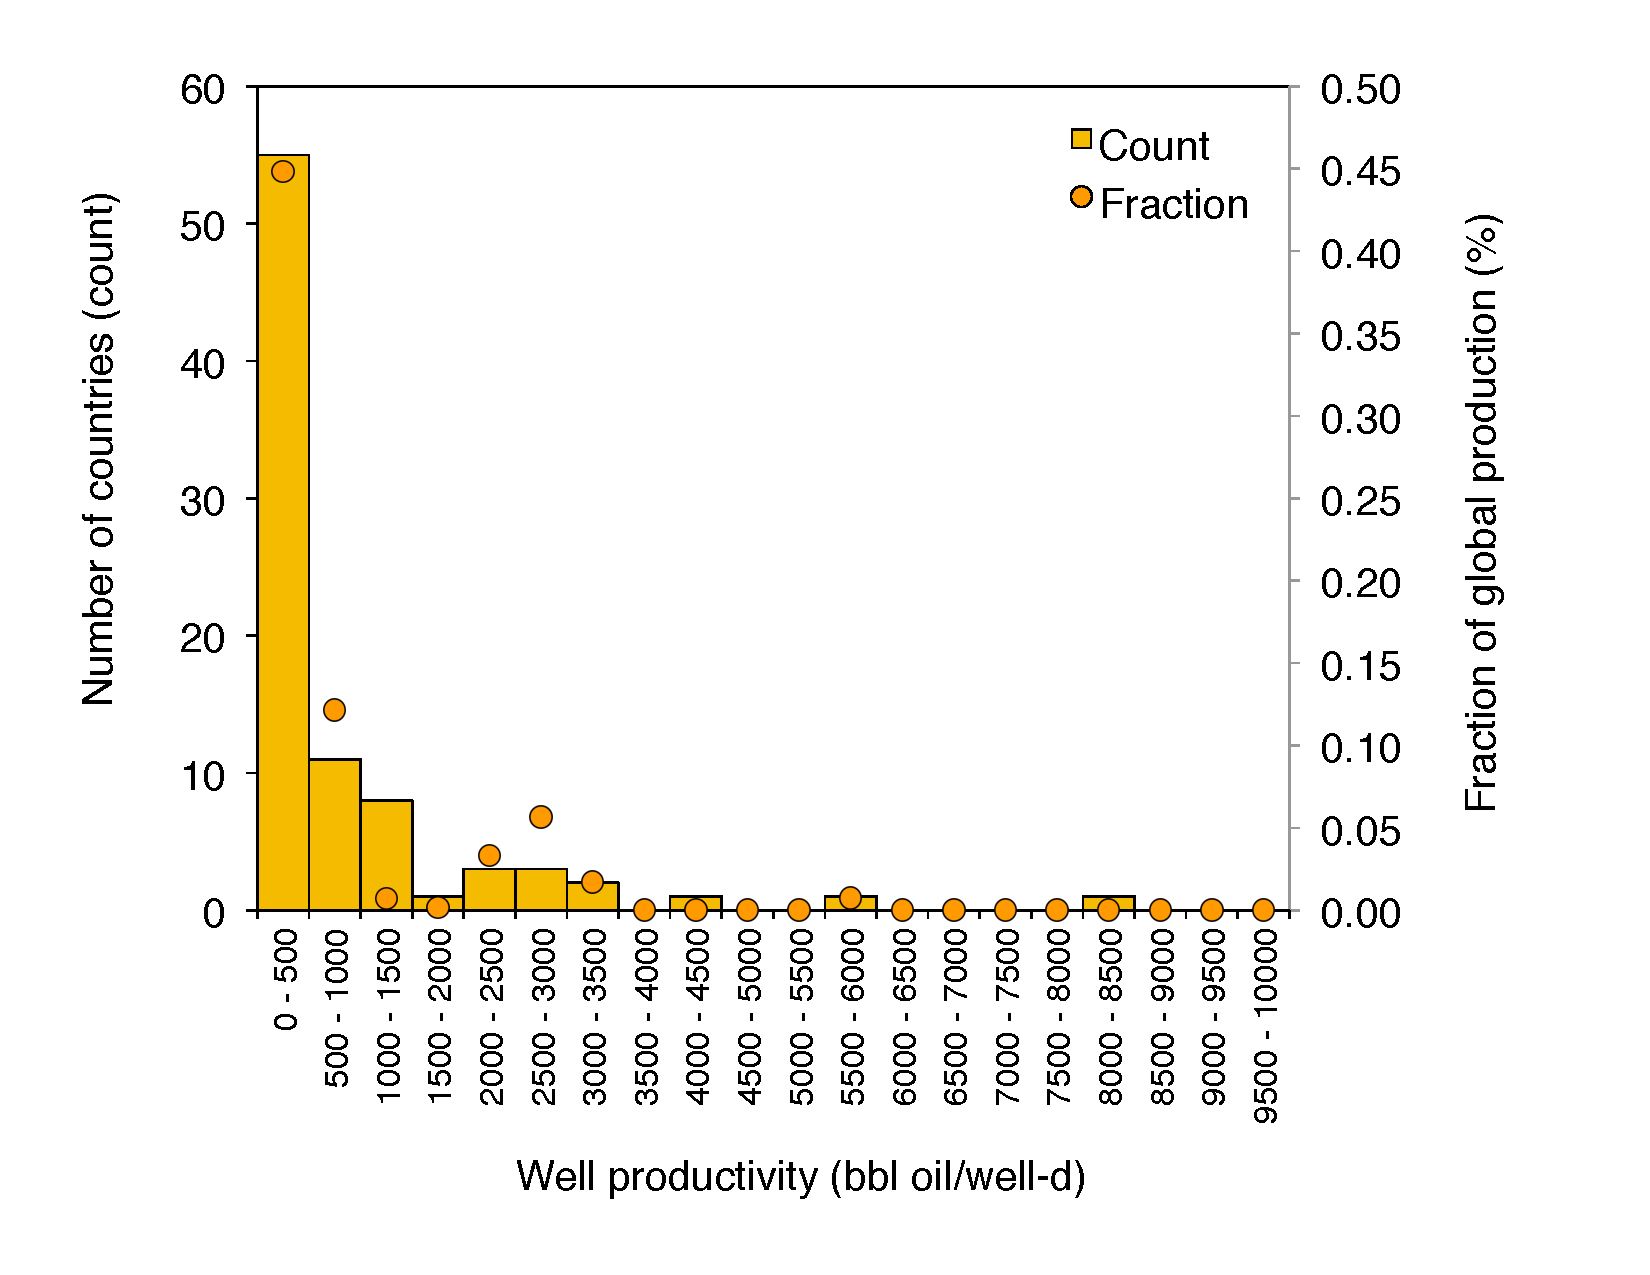
\includegraphics[width=0.8\columnwidth]{images/well_prod_all.pdf}
\caption{Distributions of oilfield per-well productivity (bbl oil/well-d) for bins of 500 bbl/d, counted by numbers of countries (bar) and by fraction of production (dot) $N$ = 92 countries.}
\label{fig:productivity_distribution_all}
\end{figure}

\begin{figure}[t]
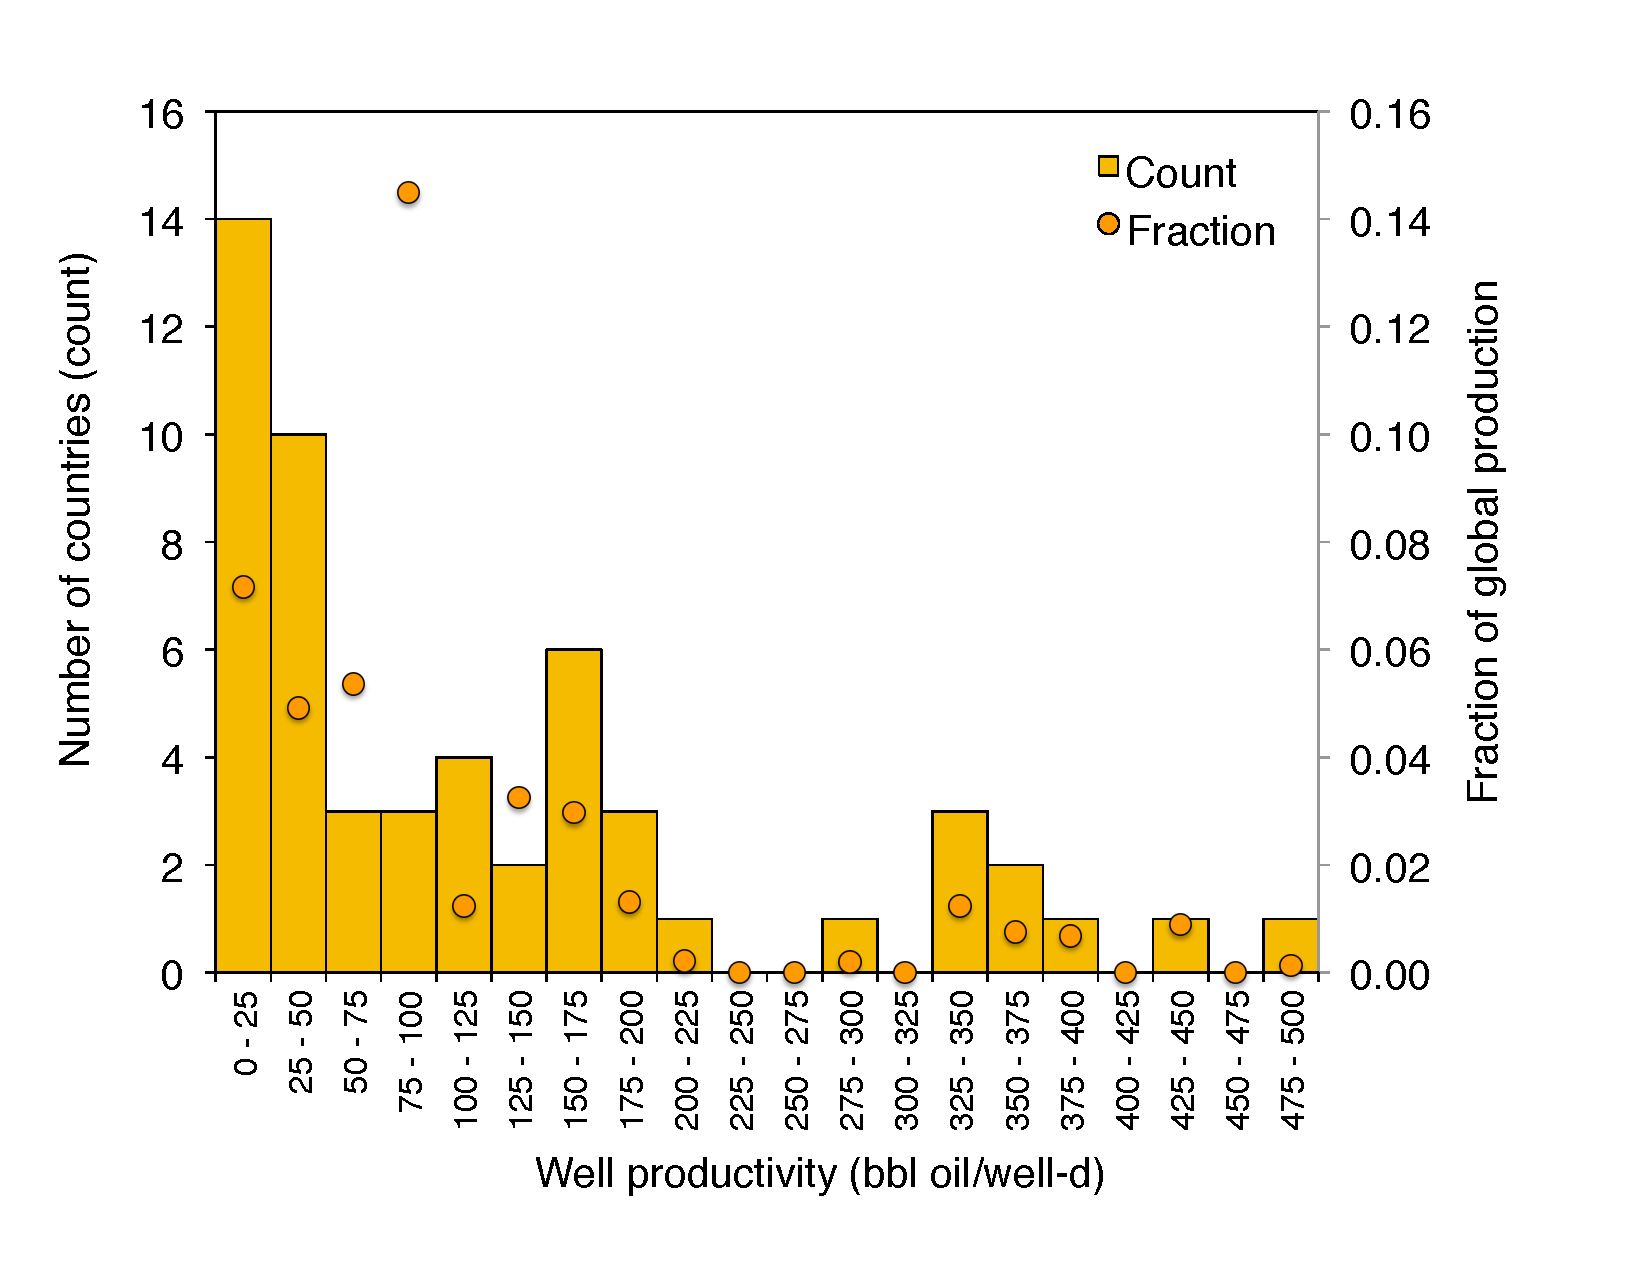
\includegraphics[width=0.8\columnwidth]{images/well_prod_low.pdf}
\caption{Distributions of oilfield per-well productivity (bbl oil/well-d) for all countries with per-well productivities lower than 500 bbl/well-d, counted by numbers of countries (bar) and by fraction of production (dot) $N$ = 55 countries.}
\label{fig:productivity_distribution_low}
\end{figure}

\subsubsection{Default number of injector wells}

The default number of injector wells is a smart default based on the number of producing wells. To model this relationship, data from California, Alaska, and a variety of offshore fields was collected \cite{DOGGR2011, AOGCC2012a}. Data from offshore fields is provided in Table \ref{tab:offshore_inj_prod} below. Per-well productivity across these fields ranges from less than 10 bbl/d to over 10,000 bbl/d.

A strong relationship is seen between the productivity of producing wells and the number of injection wells required. Highly productive wells require a significantly larger number of injectors. Figure \ref{fig:inj_prod} shows the relationship between the per-well productivity of a field and the ratio of injectors to producers.

From these data, a relationship was generated for the mean and median ratio for each logarithmic bin of production well productivity (see Table \ref{tab:inj_prod_ratios}). \marginnote{Active Field 2.2.7} Median values for each bin are used to define the smart default for the number of injector wells.

\begin{table}
\begin{scriptsize}
\caption{Mean and median injector to producer ratios.}
\label{tab:inj_prod_ratios}
\begin{tabular*}{0.75\columnwidth}{p{0.4\columnwidth}p{0.2\columnwidth}p{0.2\columnwidth}}
\toprule
Prod. well productivity & Mean & Median \\
\midrule
0-10 bbl/d & 0.193 & 0.143 \\
10 - 100 bbl/d & 0.326 & 0.254 \\
100 - 1000 bbl/d & 0.578 & 0.532 \\
$>$ 1000 bbl/d & 0.716 & 0.831 \\
\bottomrule
\end{tabular*}
\end{scriptsize}
\end{table}


\begin{figure}[t]
\includegraphics[width=0.8\columnwidth]{images/inj_prod.pdf}
\caption{Ratio of producers to injectors as a function of per-well productivity. Source: Various.}
\label{fig:inj_prod}
\end{figure}


\begin{landscape}
\begin{table}
\begin{scriptsize}
\caption{Data on production, number of production wells, and number of injection wells by offshore field.}
\label{tab:offshore_inj_prod}
\begin{tabular*}{1\columnwidth}{p{0.1\columnwidth}p{0.03\columnwidth}p{0.03\columnwidth}p{0.05\columnwidth}p{0.65\columnwidth}}
\toprule
Field & Prod. wells &Inj. wells & Prod. (bbl/d) &References \\
\midrule
Dalia &37 &31 &240000 &\url{http://www.offshore-technology.com/projects/dalia/} \\
Gimboa &3 &4 &14000 &\url{http://www.statoil.com/en/OurOperations/TradingProducts/CrudeOil/Crudeoilassays/PagPa/Gimboa.aspx}
\url{http://www.offshore-technology.com/projects/gimboa/} \\
Girassol &23 &13 &240000 &\url{http://www.offshore-technology.com/projects/girassol/} \\
Plutonio &20 &20 &240000 &\url{http://www.offshore-technology.com/projects/greater_plutonio/} \\
Hungo &30 &26 &130000 &\url{http://www.exxonmobil.com/crudeoil/about_crudes_hungo.aspx}
\url{http://www.fluor.com/projects/Pages/ProjectInfoPage.aspx?prjid=93} \\
Kissanje &25 &21 &150000 &\url{http://www.exxonmobil.com/crudeoil/about_crudes_kissanje.aspx} 
\url{http://www.ogj.com/articles/print/volume-103/issue-38/special-report/kizomba-b-attains-production-capacity-early.html} \\
Mondo &17 &17 &65000 &\url{http://www.exxonmobil.com/crudeoil/about_crudes_mondo.aspx}
\url{http://www.offshore-technology.com/projects/kizomba/} \\
Pazflor &25 &22 &220000 &\url{http://www.exxonmobil.com/crudeoil/about_crudes_pazflor.aspx}
\url{http://www.ship-technology.com/projects/pazflor-fpso/} \\
Azeri &58 &25 &823000 &\url{http://crudemarketing.chevron.com/crude/central_asian/azeri.aspx}
\url{http://www.bp.com/genericarticle.do?categoryId=9029616&contentId=7067613} \\
Albacora Leste &16 &14 &180000 &Albacora Leste Field Development Project, Offshore Technology Conference, 2006 (OTC 17925) \\
Bijupira &9 &6 &70000 &\url{http://www.offshore-technology.com/projects/bijupira/} \\
Frade &11 &4 &65000 &\url{http://www.offshore-technology.com/projects/fradefieldcamposbasi/} \\
Jubarte &20 &7 &180000 &\url{http://www.epcengineer.com/}
\url{http://subseaiq.com/data/Project.aspx?project_id=764&AspxAutoDetectCookieSupport=1} \\
Lula &5 &2 &100000 &\url{http://subseaiq.com/data/Project.aspx?project_id=274} \\
Marlim &102 &50 &390000 &\url{http://www.offshore-technology.com/projects/marlimpetro/} \\
Marlim Sul &41 &34 &300000 &\url{http://uk.reuters.com/article/2011/06/02/petrobras-platform-idUKN0227875420110602} 
\url{http://subseaiq.com/data/Project.aspx?project_id=371} \\
Polvo &10 &3 &30000 &\url{http://www.offshore-mag.com/articles/print/volume-68/issue-3/production-operations/devon-breaks-new-ground-at-polvo.html} \\
Roncador &40 &24 &460000 & \url{http://subseaiq.com/data/Project.aspx?project_id=348} \\
Sapinhoa &10 &10 &120000 & \url{http://www.offshore-technology.com/projects/guaraoilfield/} \\
\bottomrule
\end{tabular*}
\end{scriptsize}
\end{table}
\end{landscape}



\subsubsection{Default gas composition}

The default gas composition for associated gas from oil production is derived from reported gas composition data from 135 California oil fields \cite{Lee2011}. Species concentration distributions for major gas species is shown in Figure \ref{fig:gas_comp_major}. In order to remove outliers, all compositions with methane concentration less than 50\% were removed from the dataset (17 data points removed out of 135). \marginnote{Active Field 2.3.2}The resulting mean compositions were rounded and used in OPGEE for default gas composition.

\begin{figure}
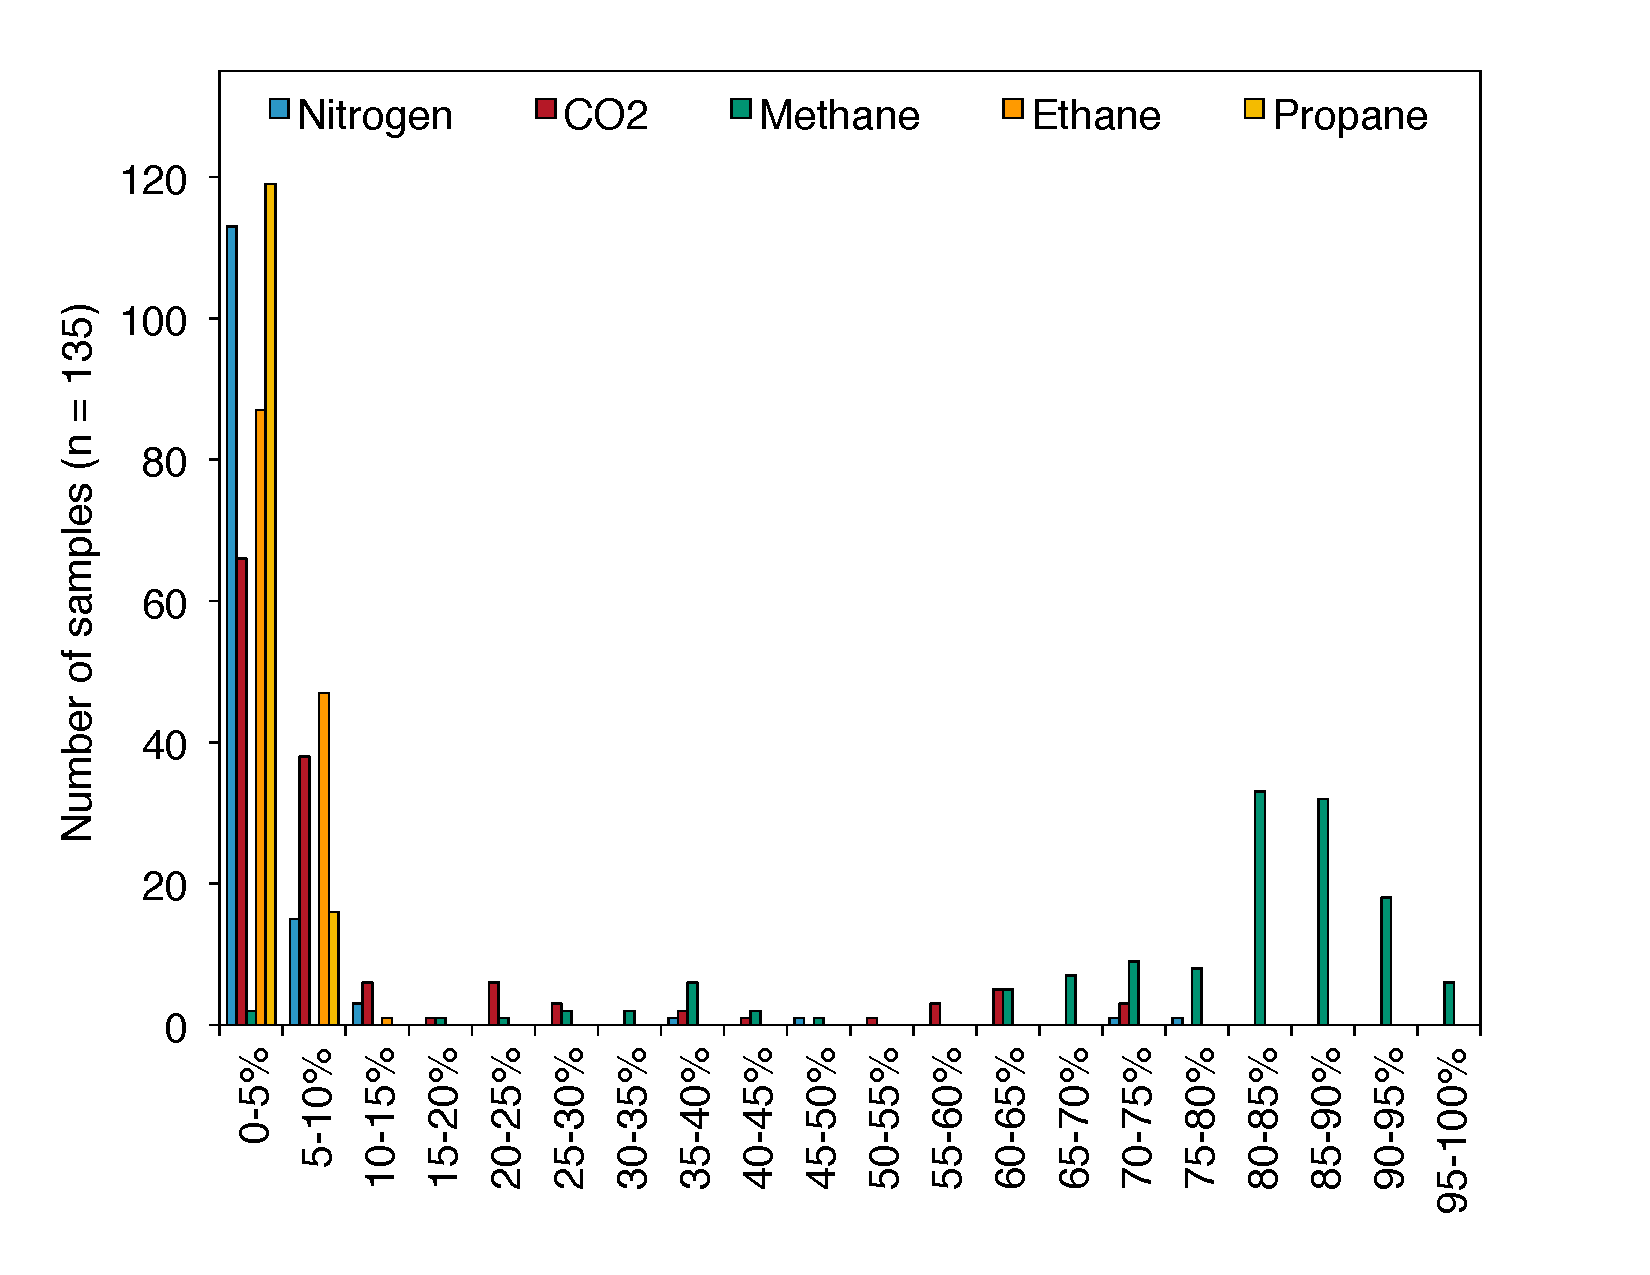
\includegraphics[width=0.8\columnwidth]{images/gas_comp_major.pdf}
\caption{Distributions of major gas species across 135 samples from California associated gas producers.}
\label{fig:gas_comp_major}
\end{figure}

\subsubsection{Smart default for GOR} \label{sec:GOR_default}

The gas-oil ratio (GOR) varies over the life of the field. The amount of gas able to be evolved from crude oil depends on its API gravity, the gas gravity, and the temperature and pressure of the crude oil \cite[p. 297]{Mccain1990}. As the reservoir pressure drops, increasing amounts of gas evolve from the liquid hydrocarbons (beginning at the bubble point pressure if the oil is initially undersaturated) \cite{Mccain1990}. This tends to result in increasing producing GOR over time. Also, lighter crude oils tend to have a higher GOR. 

Because of this complexity, a static single value for GOR is not desirable. However, all data required to use empirical correlations for GOR is not likely to be available for all crude oils modeled. \marginnote{Active Field 2.4.1} Therefore we use California producing GORs to generate average GORs for three crude oil bins. 

Crude oils are binned by API gravity into heavy ($<$ 20 $^\circ$API), medium ($\geq$ 20, $<$ 30 $^\circ$API), and light crude ($\geq$ 30 $^\circ$API). Each California oil field is assigned an average API gravity using the following procedure:
\begin{enumerate}
\item API gravity by pool is collected from DOGGR datasets \cite{DOGGR1982, DOGGR1992, DOGGR1998} and digitized.
\item If a range of API gravities is given for a single pool, the high and low specific gravities are averaged to obtain a single specific gravity value per pool, which is then converted back to API gravity.
\item The above steps give a set of single API values by pool. Each field has between 1 and 17 pools that have data in DOGGR field properties datasets.
\item Each field is assigned an average API gravity using the following method: a) if a single pool API value is given for the field, that is used; b) if multiple pool API gravities are given, and production data are available by pool, the pools are weighted by production level in 2009 DOGGR annual data (again by first converting to specific gravity then converting back to API gravity).
\item The above procedure results in a single API gravity for each field in California.
\end{enumerate}

The associated gas GOR for 179 California oil fields was compiled for 2009 \cite{DOGGRonline, DOGGRmonthly2010}. These data are binned as above based on their weighted average API gravity value. Outliters with GOR in excess of 10,000 scf/bbl were removed. The distributions, mean, and median values for each crude bin were generated (see Figure \ref{fig:API-GOR} for plot of distributions and Table \ref{tab:GOR_averages} for listing of mean and median GORs by bin).

The mean GORs are used to assign a smart default for each bin.

\begin{figure}
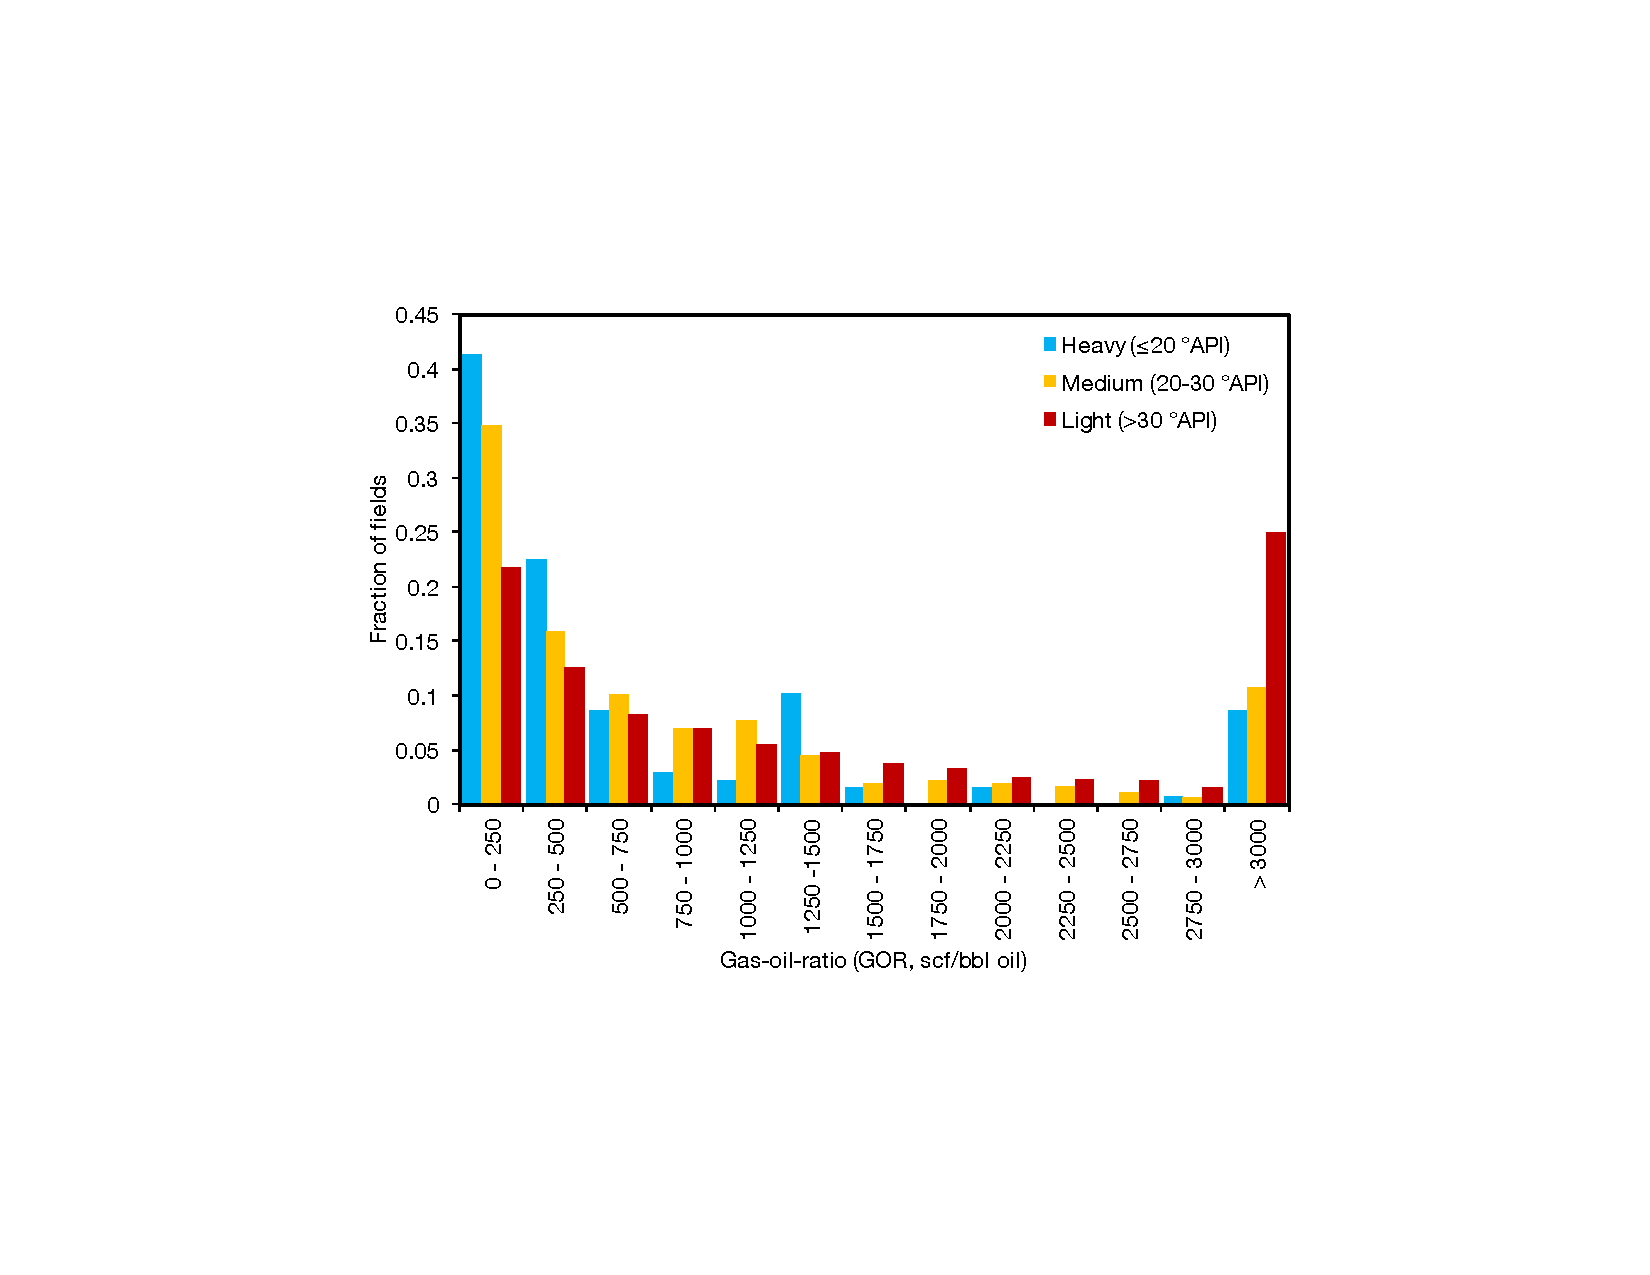
\includegraphics[width=0.8\columnwidth]{images/API-GOR.pdf}
\caption{Distributions of California GORs, binned by crude density.}
\label{fig:API-GOR}
\end{figure}


\begin{table}
\begin{scriptsize}
\caption{GOR values by crude oil API gravity bin.}
\label{tab:GOR_averages}
\begin{tabular*}{0.85\columnwidth}{p{0.15\columnwidth}p{0.08\columnwidth}p{0.15\columnwidth}p{0.1\columnwidth}p{0.1\columnwidth}p{0.1\columnwidth}}
\toprule
Crude bin & Num. fields & Gravity range & Avg. gravity & Mean GOR & Median GOR \\
& [\#] & [$^\circ$API] & [$^\circ$API] & [scf/bbl] & [scf/bbl] \\
\midrule
Heavy & 45 & $<$ 20 & 15.3 & 227 & 8 \\
Medium & 69 & $\geq$ 20, $\leq$ 30 & 24.3 & 908 & 621 \\
Light & 65 & $>$ 30 & 35.0 & 1297 & 877 \\
\bottomrule
\end{tabular*}
\end{scriptsize}
\end{table}


\subsubsection{Default water oil ratio (WOR)} \label{WORSmartDefault}

A smart default for the water oil ratio as a function of field age was generated using data from large fields in various world regions. \marginnote{Active Field 2.4.2}

Data on oil and water production were extracted from reports issued by California Division of Oil, Gas and Geothermal Resources (DOGGR), Alberta Energy Resources Conservation Board (ERCB), Alaska Oil and Gas Conservation Commission (AOGCC), United Kingdom Department of Energy and Climate Change (DECC), and the Norwegian Petroleum Directorate (NPD). For the Norwegian fields, water production data were not available prior to the year 2000. For Alberta fields, data were not available prior to 1962. Only data for the first 60 years of production were included. Only California fields contained data beyond 55 years, and therefore we excluded these years to avoid possibly atypical depleted field behavior in California from significantly affecting the least squares fit. 

Because the majority of crude oil that is marketed globally originates from larger oil fields, fields that have produced less than 100 million m$^3$ (630 million bbl) of crude oil were excluded. Also excluded from the analysis were fields that produce heavy crude using steam injection. 

Additionally, a small number of fields were excluded because of apparent data anomalies or unusual events that may have affected oil or water production. Both the Redwater field in Alberta and the Ninian field in UK North Sea were excluded for data anomalies. These fields have highly unusual water production data that can only be plausibly attributed to data entry error. Also, the Elk Hills field in California was excluded because it was part of the National Petroleum Reserve for many years and the Piper field in the UK was excluded because oil production was halted for several years. In total, data from 24 giant oil fields (10 onshore and 14 offshore) were included in the analysis. The largest and the only super-giant field to be included is Prudhoe Bay.


The default WOR is represented by an exponential function:
%%%%%%%%%%
\begin{equation}\label{eq:smart_default_WOR}
WOR(t) = a_{WOR} \exp [b_{WOR} ( t - t_0 )] - a_{WOR} \quad\quad \footnotesize{\left[\frac{\text{bbl water}}{\text{bbl oil}}\right]}
\end{equation}
%%%%%%%%%%
where $a_{WOR}$ = fitting constant for the initial WOR in time = $t_0$ [bbl water/bbl oil]; $b_{WOR}$ = exponential growth rate [1/y]; $t_0$ = initial year of production (or year of discovery if year of first production unavailable) [y]; and $t$ = year being modeled (independent variable) [y]. Note that the pre-exponential $a_{WOR}$ is subtracted to force WOR to start at 0 when $t = t_0$. This model was fit to the collected data using a nonlinear least-squares fit from multiple starting points to ensure robustness.
The results of fitting this model to the smart default fit values, compared to oil fields from a variety of world regions, is show in figure \ref{fig:exponenital_fit_WOR}. The resulting fit gives $a_{WOR} = 1.706$ and $b_{WOR} = 0.036$.

\begin{figure}
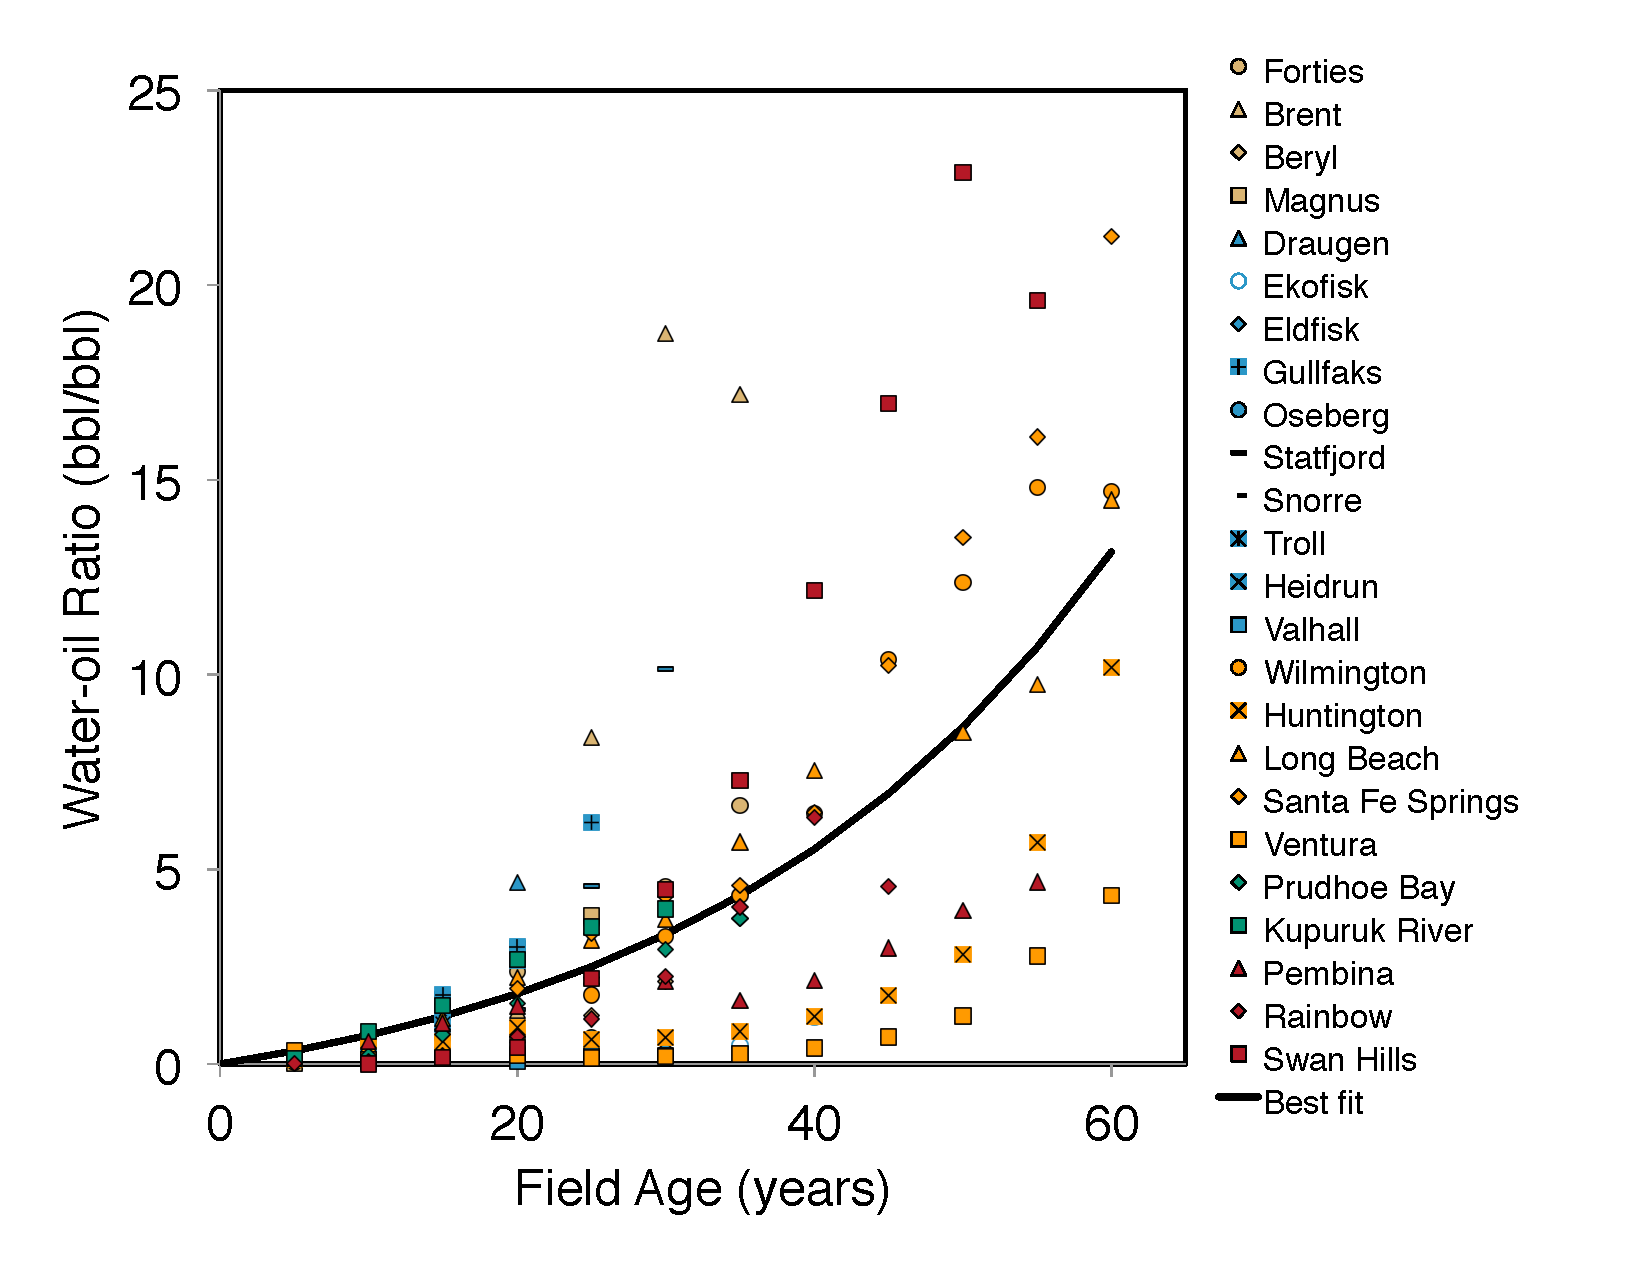
\includegraphics[width=1\columnwidth]{images/WOR_plot.pdf}
\caption{Exponential WOR model fit with smart default parameters. The best fit to data gives $a_{WOR} = 1.706$ and $b_{WOR} = 0.036$. Regions are colored as follows: Alberta (red), Alaska (green), California (orange), Norway (blue) and UK (beige).}
\label{fig:exponenital_fit_WOR}
\end{figure}

\subsubsection{Default waterflooding volume}

The volume of water injected in a waterflooding project is meant to maintain reservoir pressure. \marginnote{Active Field 2.4.3} As a default value, OPGEE assumes that the surface volume is replaced, such that the total oil produced plus the water produced is reinjected, or the injection per bbl = 1 + WOR.

\subsubsection{Default flood gas injection ratio}

This is the ratio of the volume of flood gas injected [scf] to the volume of oil produced [bbl]\marginnote{Active Field 2.4.5}. The volume of the oil is measured after bulk processing has removed the associated gas. The default flood gas injection ratio value depends on the choice of flood gas. If natural gas is selected as the flood gas, then the default ratio is calculated as follows:
%%%%%%%%%%
\begin{equation}\label{eq:NaturalGasAirOxygenFloodGasRatio}
R_{fl}=1.5\cdot GOR \quad\quad \footnotesize{\left[\frac{\text{scf gas}}{\text{bbl oil}}\right]}
\end{equation}
%%%%%%%%%%
where $R_{fl}$ = flood gas injection ratio [scf/bbl] and GOR is the gas-oil-ratio [scf/bbl].

If N$_2$ is selected as the flood gas, then $R_{fl}$ is 1,200 scf/bbl. This is based on the immiscible nitrogen flood operation at the Cantarell field in Mexico to maintain reservoir pressure. As described in the \nameref{GasFlooding} section, the field operating equipment is designed to inject 1,200 MMscf/d \cite{Kuo2001}. In 2008, the injection rate was approximately 1,200 MMscf/d and the field was producing approximately 1.2 million bbl/d, leading to a default ratio of 1,200 scf/bbl \cite{guzmann2014review}.

If CO$_2$ is selected as the flood gas, then default $R_{fl}$ is 10,000 scf/bbl. As with all injection ratios, $R_{fl}$  changes over the life cycle of the flood project. It can also vary based on the specific reservoir engineering strategies selected by the operator.  An example comes from DiPietro and Murrel (2013), who presented data from Kinder Morgan indicating that the injection ratio during the overall lifespan of an anonymous representative project was 6,000 scf/bbl. 

Another example is provided by Pyo et al. \cite{pyo2003co2}, who reviewed the performance of a CO$_2$ flood at the Joffre Viking Pool in Alberta, Canada that had been active for approximately 30 years. The overall flood gas injection ratio during the life of the project was 10,800 scf/bbl; the ratios for the individual injector-producer well patterns within the field varied from 3,500 to 24,900 scf/bbl. 

The OPGEE default flood gas injection ratios are presented only as representative values that provide an order-of-magnitude estimate. Actual field data should be obtained when possible.

\subsubsection{Proportion of injected CO$_2$ that is newly acquired}
The OPGEE default for the proportion of CO$_2$ that is newly acquired (not previously injected) is 41\%. This figure is from the Malone et al. \cite{NETL2014} discussion of an offshore CO$_2$ flood project at Weeks Island, Louisiana over an 9-year period (based on dates in the original reference by Johnston \cite{johnston1988weeks}). As with the flood gas injection ratio, actual data should be used if possible. 

\subsubsection{Default for steam-oil-ratio (SOR)}

Because the SOR is a key parameter driving GHG emissions from thermal oil production operations, we examine default values for SOR in more detail. 

SOR data are collected for California and Alberta thermal oil recovery operations for 2010 and 2011 \cite{DOGGR2010, DOGGR2011, DOGGRmonthly2010, ERCB2010, ERCB2011a}. 

For California operations, incremental SOR is calculated for 2009 using volumes of steam injected and reported incremental production due to steam injection. `Total' SOR is also calculated for 2009 using total production by field and total steam injection. For 2010, only monthly data are available, so incremental production data are not available. Therefore, only total SOR is reported.

For Alberta operations, data on bitumen produced and steam injected were collected for 24 thermal recovery projects (SAGD and CSS). No data were available on incremental rather than total production, and it is not clear what incremental production figures would represent bitumen operations where non-enhanced production would be very small.

Production volumes are binned by SOR for both regions and reported in Figure \ref{fig:SOR_dist}. Averages for SOR are presented in Table \ref{tab:SOR_stats}.  The default SOR in OPGEE \version \, is a conservative 3.0 bbl CWE per bbl oil. 

\begin{figure}[t]
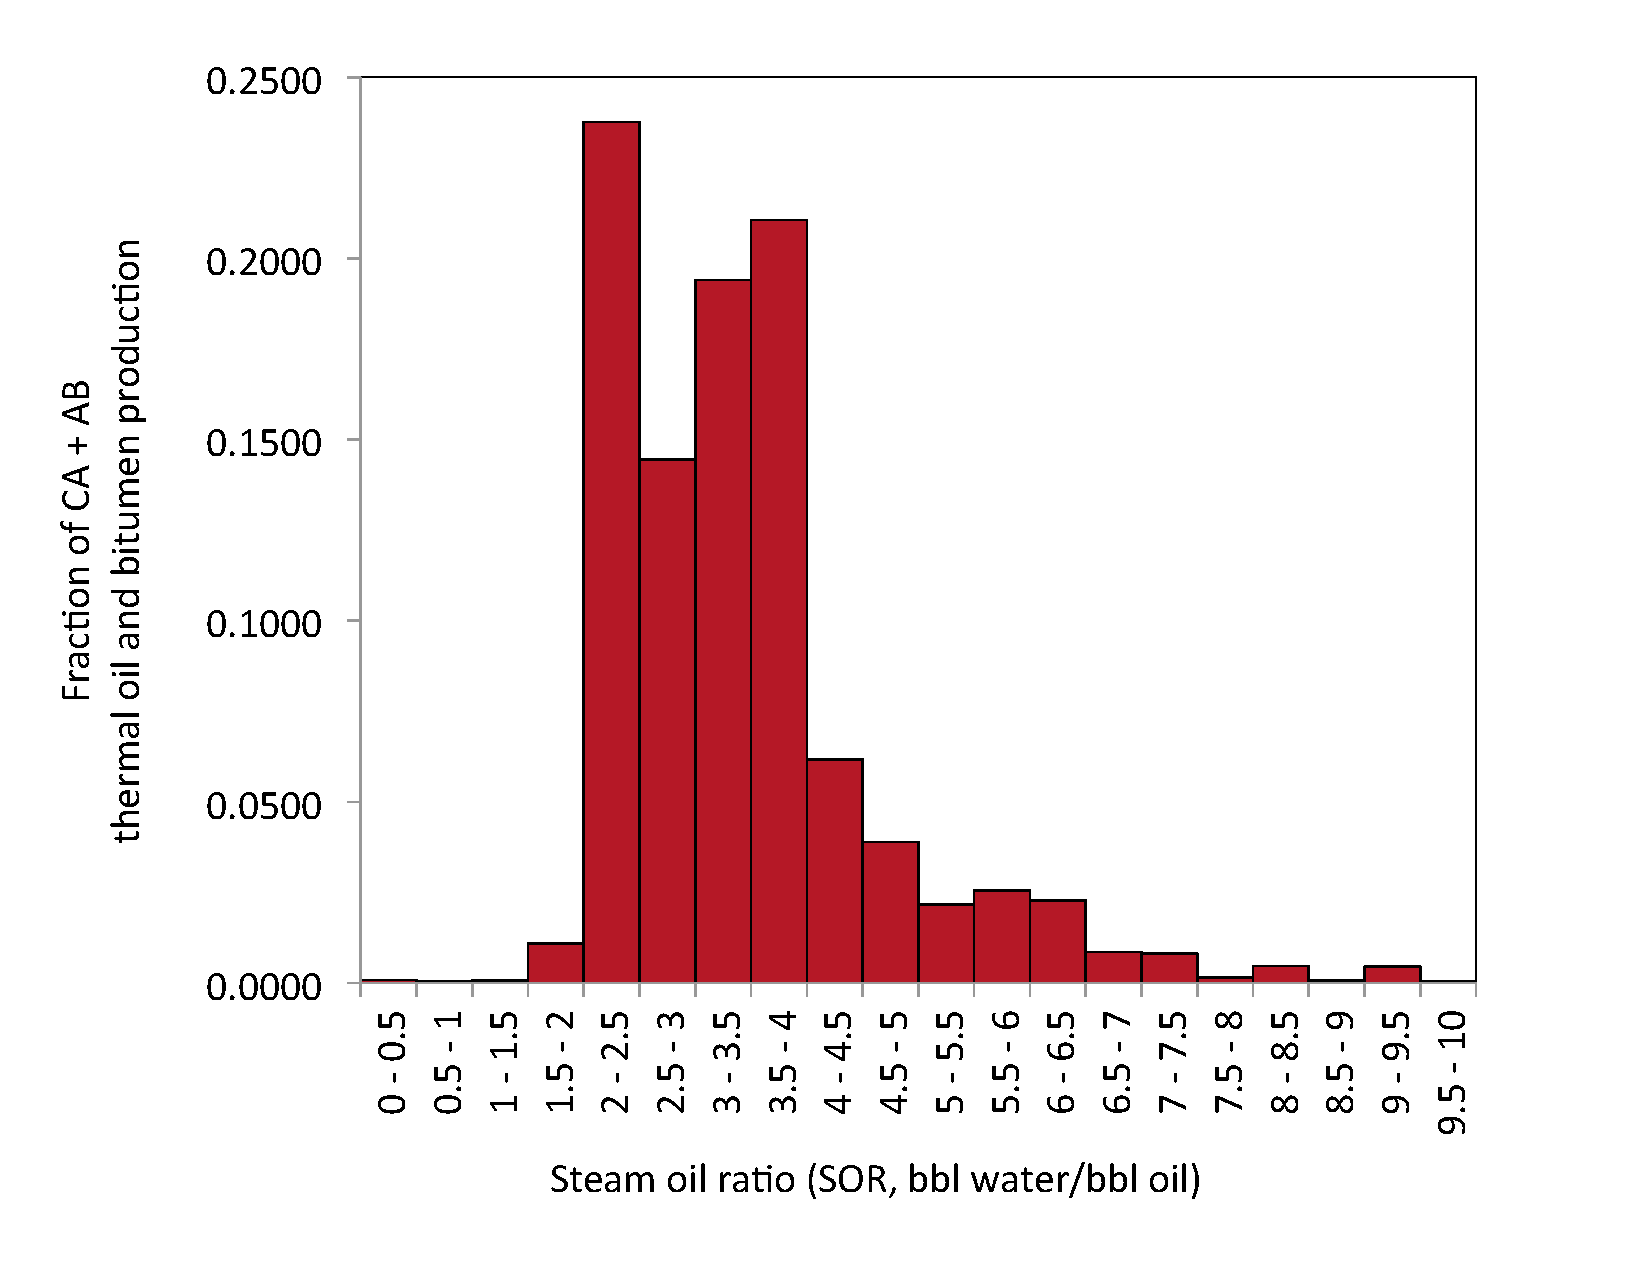
\includegraphics[width=0.85\columnwidth]{images/SOR_dist.pdf}
\caption{Distribution of SOR values for California and Alberta thermal EOR projects (steamflood, cyclic steam stimulation, steam-assisted gravity drainage).}
\label{fig:SOR_dist}
\end{figure}


\begin{table}
\caption{Indicators of SOR distributions for California and Alberta thermal EOR production. Units are bbl of cold water equivalent (CWE) per bbl of oil.}
\label{tab:SOR_stats}
\begin{scriptsize}
\begin{tabularx}{1\columnwidth}{p{0.3\columnwidth}p{0.15\columnwidth}p{0.15\columnwidth}}
\toprule
& Mean - SOR$_t$ & Mean - SOR$_i$ \\
\midrule
California - 2009 & 3.32 & 4.29 \\
California - 2010 & 3.41 & Unk. \\
Alberta - 2009 & 3.58 & NA \\
Alberta - 2010 & 3.32 & NA \\
\bottomrule
\end{tabularx}
\end{scriptsize}
\end{table}




%%%%%%%%%%%%%%%%%%%%%%%%%%%%%%%%%%%%%%%%%%%%%
%%%%%%%%%%%%%%%%%%%%%%%%%%%%%%%%%%%%%%%%%%%%%
%%%%%%%%%%%%%%%%%%%%%%%%%%%%%%%%%%%%%%%%%%%%%

\chapter{Flow sheet}


\clearpage

%%%%%%%%%%%%%%%%%%%%%%%%%%%%%%%%%%%%%
\section{Flow sheet introduction}\label{sec:gas_balance}

The flow sheet is the main organizing sheet for OPGEE. It includes graphical representation of the process flows and numerical results for all streams in all phases. The streams are numbered 1-300 (with gaps for forward compatability). At the top of the table, each stream contains a mass flow of a given set of possible substances.  In the lower section of the flow table, a variety of other characteristics of each stream are computed. These properties are computed for all streams using equivalent formulas.

To refer to a given stream property, the ``Index'' function in Excel is used. The syntax of the Index function is as follows:
\begin{verbatim}
Index([Table],[Row],[Column])
\end{verbatim}
where \verb+[Table]+ is the name of the table being accessed, and \verb+[Row]+ and \verb+[Column]+ are the row and column of the entry desired.

In order to call a quantity from the Flow table, the proper syntax would then be:
\begin{verbatim}
Index(FlowTable,PROP_NAME,STREAM_NUM)
\end{verbatim}
where \verb+PROP_NAME+ is the name of the property desired and \verb+STREAM_NUM+ is the number of the stream of interest.

The property names are defined as follows in Table \ref{tab:stream_properties}. After Table \ref{tab:stream_properties} the method of computing each property is given below.

\begin{table}
\begin{scriptsize}
\caption{Properties computed for each stream: Symbol, description, units, and source of relevant equation.}
\label{tab:stream_properties}
\begin{tabularx}{1\columnwidth}{p{0.1\columnwidth}p{0.35\columnwidth}p{0.1\columnwidth}p{0.1\columnwidth}p{0.1\columnwidth}}
\toprule
Symbol 		&	Description		& Units		& Source		& Notes \\
\midrule
\bottomrule
\end{tabularx}
\end{scriptsize}
\end{table}



\section{Computing properties of flows}

\subsection{Mass flows}

Mass flows per day are denominated  or \xlname{M\_X} where \xlname{X} is a place holder for a given stream component [tonne/d].  The following streams are recognized in OPGEE:
\begin{itemize}
\item \xlname{PC} -- Petroleum coke streams
\item  \xlname{O} -- Oil streams
\item  \xlname{LPG} -- Liquified petroleum gas streams
\item \xlname{W} -- Water stream
\item  \xlname{N2} -- Nitrogen stream
\item  \xlname{O2} -- Oxygen stream
\item  \xlname{CO2} -- Carbon dioxide stream
\item  \xlname{H2O} -- Water vapor stream
\item  \xlname{C1} -- Methane stream
\item  \xlname{C2} -- Ethane stream
\item  \xlname{C3} -- Propane stream
\item  \xlname{C4} -- Butane stream
\item  \xlname{CO} -- Carbon monoxide stream
\item  \xlname{H2} -- Hydrogen stream
\item  \xlname{H2S} -- Hydrogen sulfide stream
\item \xlname{SO2} -- Sulfur dioxide stream
\end{itemize}

The only solid component tracked in the \sheet{Flow sheet} is petroleum coke \xlname{PC}. Petroleum coke is a solid form of primarily carbon, generated at crude oil upgrading and refining facilities. 

Three liquid components are tracked in the \sheet{Flow sheet}.  Oil streams \xlname{O} are defined as hydrocarbon streams that are liquid at standard temperature and pressure. For simplicity, bitumen is considered a liquid oil stream. Oil streams vary from API gravity of 6 $^\circ$API (heavy bitumen) to 70 $^\circ$API (light condensate or diluent). Liquified petroleum gas (LPG) streams \xlname{LPG} is a stream that is gaseous at ambient temperature and pressure but will liquify at low pressures and therefore is commonly transported in dense form (commonly mixtures of mostly propane and butane). Water \xlname{W} can be brackish or fresh water.

Twelve gas components are tracked in the \sheet{Flow sheet}. These include consituents of air (\xlname{N2}, \xlname{O2}, \xlname{CO2}, and \xlname{H2O}). Note that water vapor is represented by \xlname{H2O} while liquid phase water is tracked as \xlname{W}.  Next are the four light hydrocarbons, \xlname{C1} - \xlname{C4}. Some sources distinguish a species in gas called ``pentanes plus''. Given that these are liquid a standard temperature and pressure, these would be considered a very light oil stream. Similarly, lease condensate and natural gas plant liquids are also tracked as oil \xlname{O}. Lastly, minor constituents are tracked: \xlname{CO}, \xlname{H2}, \xlname{H2S}, and \xlname{SO2}.


\subsection{Electricity flows}

Electricity is tracked by its energy flow rate per day [MWh/d] \xlname{E\_EL}. No distinction is made between high voltage or low voltage electricity, nor do we distinguish between DC and AC power.

\subsection{Properties of phases}

Certain properties are tracked for the composite of all phases in the stream.  These include temperature [$^\circ$F] \xlname{T}, absolute temperature  [$^\circ$R], \xlname{T\_ABS}, pressure [psia] \xlname{P}.

Each stream is also classified as containing oil \xlname{OIL\_01}, containing liquid phase water \xlname{WAT\_01}, and containing gases \xlname{GAS\_01}. These are 0-1 binary variables used in logical flows for computing properties of different streams.

\subsection{Properties of oil}

A number of properties of oil are tracked.  These properties are a function of oil chemistry (heating value) as well as the temperature and pressure of the stream (solution gas oil ratio).

\paragraph{API gravity of oil}

The API gravity of the oil is tracked as variable \xlname{API\_O}.  For conventional oil streams, this is defined as equal to the defined parameter \xlname{API\_grav} (streams given in Table \ref{tab:Source_API_Gravity}).  For bitumen streams it is equal to defined parameter \xlname{Bitumen\_API}.  For diluent streams it is equal to \xlname{Diluent\_API}. For LPG the API gravity is not computed as this parameter is not typically used to represent these products.

\begin{table}
\begin{scriptsize}
\caption{Source of API gravity for oil streams.}
\label{tab:Source_API_Gravity}
\begin{tabularx}{1\columnwidth}{p{0.05\columnwidth}p{0.35\columnwidth}p{0.2\columnwidth}p{0.1\columnwidth}p{0.1\columnwidth}}
\toprule
Stream num. & Stream name	&	Source of API gravity term		& Default		& Notes \\
\midrule
\stream{1}			& Crude oil in reservoir	& \xlname{API\_grav}				& 30$^\circ$ API &  \\
\stream{2}			& Bitumen in mine		& \xlname{API\_Bitumen}				& 30$^\circ$ API &  \\
\stream{3}			& Crude oil at well bottom	& \xlname{API\_grav}				& 30$^\circ$ API &  \\
\stream{4}			& Crude oil at wellhead	& \xlname{API\_grav}				& 30$^\circ$ API &  \\
\stream{5}			& Bitumen from mine to upgrader	& \xlname{API\_Bitumen}		& 30$^\circ$ API &  \\
\stream{6}			& Bitumen from mine to dilution	& \xlname{API\_Bitumen}			& 30$^\circ$ API &  \\
\stream{7}			& Crude oil after separator	& \xlname{API\_grav}			& 30$^\circ$ API &  \\
\stream{8}			& Crude oil to stabilizer	& \xlname{API\_grav}				& 30$^\circ$ API &  \\
\stream{9}			& Crude oil to storage	& \xlname{API\_grav}				& 30$^\circ$ API &  \\
\stream{10}		& Stabilized crude to storage	& \xlname{API\_grav}			& 30$^\circ$ API &  \\
\stream{11}		& Upgraded crude to storage	& \xlname{API\_grav}			& 30$^\circ$ API &  \\
\stream{12}		& Diluted bitumen to storage	& \xlname{API\_grav}			& 30$^\circ$ API &  \\
\stream{13}		& Crude oil to transport	& \xlname{API\_grav}				& 30$^\circ$ API &  \\
\stream{14}		& Transported crude oil at refinery	& \xlname{API\_grav}				& 30$^\circ$ API &  \\
\stream{15}		& Petcoke export from upgrader	& -				& - &  \\
\stream{16}		& NGL/diluent to dilution	& \xlname{API\_diluent}				& 30$^\circ$ API &  \\
\stream{17}		& LPG to blend with crude oil	& \xlname{API\_diluent}				& 30$^\circ$ API &  \\
\stream{18}		& LPG to direct sales	& \xlname{API\_diluent}				& 30$^\circ$ API &  \\
\stream{19}		& Crude oil to upgrader	& \xlname{API\_grav}				& 30$^\circ$ API &  \\
\stream{20}		& Crude oil in dilution	& \xlname{API\_grav}				& 30$^\circ$ API &  \\
\bottomrule
\end{tabularx}
\end{scriptsize}
\end{table}

\paragraph{Specific gravity of oil}

The specific gravity of the oil is tracked as variable \xlname{GAMMA\_O}. It is computed from the API gravity as follows:
\begin{equation}
\gamma_o = \frac{141.5}{131.5 + API} \eqnunitfrac{g}{g}.
\end{equation}
\begin{equation}
\xlname{GAMMA\_O} = \frac{141.5}{131.5 + \xlname{API\_O}} \eqnunitfrac{g}{g}.
\end{equation}

This equation holds for conventional oil, bitumen, and diluent. For LPG streams the density is assumed equal to 550 kg/$m^3$, or midway between the density of propane (504 kg/m$^3$ at 60 $^\circ$F) and butane (600 kg/m$^3$ at 60 $^\circ$F).

\paragraph{Solution gas oil ratio of oil}

The solution gas oil ratio $R_s$ \xlname{GOR\_OS} is the amount of gas in solution in a crude oil as a function of a number of properties. If there is more gas present than this amount, the gas will start to evolve from the oil into a separate gas phase (i.e., the gas will start to bubble out of the oil).  As recommended in Fanchi \cite{Fanchi2007}, we re-arrange the bubblepoint pressure relationship to solve for the amount of gas in solution at a given pressure. We use the bubblepoint pressure relationship of Al-Shammasi (1999), as reproduced in \cite[vol 1, Table 6.6]{Fanchi2007}:
\begin{equation}
R_{s} = \frac{p^{\left(\frac{1}{a_2}\right)} \gamma_{o}^{\left(-\frac{a_1}{a_2}\right)} e^{\left(\frac{a_3}{a_2} \gamma_o \gamma_g\right)}}{\gamma_g T_{abs}} \eqnunitfrac{scf}{bbl}
\label{eq:GOR_OS}
\end{equation}
If the resulting gas oil ratio is larger than the bubblepoint pressure gas oil ratio ($R_b$), then the equation defaults to the bubblepoint gas oil ratio. The equation for bubblepoint gas oil ratio is given below in Eq. \ref{}.


\paragraph{Oil formation volume factor}

The oil formation volume factor $B_o$ \xlname{OVF} is the ratio of the number of barrels that a barrel of oil will occupy in the reservoir over the number of stock tank (standard) barrels that the oil will occupy. The oil formation volume factor is a function of the solution gas oil ratio, the temperature, and the pressure of the fluid, with the gas in solution being the largest determinant. The oil FVF at the bubblepoint pressure is generated via bubblepoint oil FVF correlations \xlname{FVF\_SAT}. We use the bubblepoint oil formation volume factor correlation from Al-Shammasi \cite[Table A-3, p. 317]{Fanchi2007}\cite{Alshammasi1999}:
\begin{equation}
B_{ob} = a_1+ a_2 R_s (T_r - 60) + a_3\left( \frac{R_s }{\gamma_o}\right) + a_4  \left(\frac{T_r - 60}{\gamma_o}\right)+ a_5 R_s \left( \frac{\gamma_g}{\gamma_o}\right)  \eqnunitfrac{bbl}{STB}
\label{eq:BOB}
\end{equation}
this correlation is useful for saturated oil, or oil with its associated gas at the maximum amount (i.e., as pressure drops gas is evolved). 

For undersaturated oil, oil holds less gas in solution than it could at that temperature and pressure. In this case the pressure is above the bubblepoint pressure and the oil formation volume factor varies using a different functional form. The undersaturated oil FVF \xlname{FVF\_UNSAT} is:
\begin{equation}
B_o = B_{ob} e^{[c_o (p_b-p)]} \eqnunitfrac{bbl}{STB}
\label{eq:BO}
\end{equation}
where $c_o$ is the isothermal compressibility of oil, $p_b$ the bubblepoint pressure of oil, and $p$ the pressure of the stream.

We use the correlation of Al-Mahoun \cite{Almahoun1992} for the isothermal compressibility term \cite[Table A-5, p. 320]{Fanchi2007}. First, term $X$ is computed \xlname{ISO\_X}:
\begin{equation}
X = a_1R_s + a_2 R_s^2 + a_3 \gamma_g  + a_4 (T_{abs})^2  \eqnunit{-}
\label{eq:X_ISO}
\end{equation}
where $R_s$ is the solution gas oil ratio [scf/bbl], $\gamma_g$ is the gas specific gravity [-] and $T_{abs}$ is the absolute temperature [$^\circ$R]. From this term the isothermal compressibility $c_o$ \xlname{ISO\_CO} can be computed as:
\begin{equation}
c_o = \frac{X \, \ln\left(\frac{p}{p_b}\right)}{p_b-p} \eqnunitfrac{1}{psi}
\label{eq:CO_ISO}
\end{equation}
Finally, we can uses these two terms to compute the oil FVF \xlname{FVF\_UNSAT}. If $p<p_b$, $B_{ob}$ is used, while if $p \geq p_b$ then $B_o$ is used.


\paragraph{Density of oil}

Using the above terms, the density of crude \xlname{RHO\_O\_LB} can then be computed in using the following relation \cite[p. 277]{Fanchi2007}:
\begin{equation}
\rho_o = \frac{a_1 \gamma_{o}+ a_2 \gamma_{g} R_{s}}{B_o} \eqnunitfrac{lbm}{ft$^3$}
\label{eq:rho_o}
\end{equation}
where $\gamma_g$ is the specific gravity of gas (defined below in Eq. \ref{}) and $a_1$ and $a_2$ are the densities of water and air at standard conditions. This value is also converted to SI units [kg/m$^3$] \xlname{RHO\_O}. For LPG the density is assumed to be 550 kg/m$^3$.

\paragraph{Volumetric flow rate of oil}
The volumetric flow rate of oil is then given by the mass flow rate $m_o$ and the density of crude oil:
\begin{equation}
Q_o = \frac{m_o}{\rho_o}  \eqnunitfrac{m$^3$}{d}
\end{equation}

\paragraph{Energy density of oil}

The energy density (heating value per unit mass) of oil is computed using a polynomial correlation for LHV of crude as a function of crude API gravity from the API Technical Databook, eq. 14A1.3-3:
\begin{equation}
LHV_o = a_1 + a_2 API - a_3 API^2 - a_4 API^3  \eqnunitfrac{btu LHV}{lbm}
\label{eq:LHVO}
\end{equation}
This is then converted to SI units [MJ/kg]. A similar polynomial function can be used to compute the HHV of oil as a function of API gravity:
\begin{equation}
HHV_o = a_1 + a_2 API - a_3 API^2 - a_4 API^3  \eqnunitfrac{btu HHV}{lbm}
\label{eq:HHVO}
\end{equation}
For LPG streams the energy density is assumed equal to 50 MJ/kg.

\paragraph{Energetic flow rate of oil}

The energetic flow rate of oil can then be computed using the above terms:
\begin{equation}
F_{LHV,o} = Q_o  LHV_o
\end{equation}




\begin{table}
\begin{scriptsize}
\caption{Constants in equations for liquid stream properties.}
\label{tab:ConstantsLiquidFlowSheet}
\begin{tabularx}{1\columnwidth}{p{0.05\columnwidth}p{0.35\columnwidth}p{0.05\columnwidth}p{0.1\columnwidth}p{0.2\columnwidth}p{0.1\columnwidth}}
\toprule
Eq. num. 			& Description	 			& Term		& Value  		& Units		& Source \\
\midrule
\ref{eq:GOR_OS}	& Solution gas oil ratio		& $a_1$		& 5.527215	& -			& \cite{Alshammasi1999} \\
\ref{eq:GOR_OS}	& Solution gas oil ratio		& $a_2$		& 0.783716	& -			& \cite{Alshammasi1999} \\
\ref{eq:GOR_OS}	& Solution gas oil ratio		& $a_3$		& 1.841408	& -			& \cite{Alshammasi1999} \\
\midrule
\ref{eq:BOB}		& Bubblepoint oil FVF		& $a_1$		& 1			& -			& \cite{Alshammasi1999} \\
\ref{eq:BOB}		& Bubblepoint oil FVF		& $a_2$		& 5.25E-07	& -			& \cite{Alshammasi1999} \\
\ref{eq:BOB}		& Bubblepoint oil FVF		& $a_3$		& 1.81E-04	& -			& \cite{Alshammasi1999} \\
\ref{eq:BOB}		& Bubblepoint oil FVF		& $a_4$		& 4.49E-04	& -			& \cite{Alshammasi1999} \\
\ref{eq:BOB}		& Bubblepoint oil FVF		& $a_5$		& 2.06E-04	& -			& \cite{Alshammasi1999} \\
\midrule
\ref{eq:X_ISO}		& Isothermal compressibility	& $a_1$		& -1.37E-05	& [bbl/scf]			& \cite{Almahoun1992} \\
\ref{eq:X_ISO}		& Isothermal compressibility	& $a_2$		& -1.93E-08	& [bbl$^2$/scf$^2$]			& \cite{Almahoun1992} \\
\ref{eq:X_ISO}		& Isothermal compressibility	& $a_3$		& 2.41E-02	& [-]			& \cite{Almahoun1992} \\
\ref{eq:X_ISO}		& Isothermal compressibility	& $a_4$		& -9.26E-03	& [1/$^\circ$R$^2$]			& \cite{Almahoun1992} \\
\midrule
\ref{eq:rho_o}		& Density of oil				& $a_1$		& 62.428		& [lbm/ft$^3$]			& \cite{Fanchi2007} \\
\ref{eq:rho_o}		& Density of oil				& $a_2$		& 0.0136		& [lbm-bbl/ft$^3$-scf]			& \cite{Fanchi2007} \\
\midrule
\ref{eq:LHVO}		& Lower heating value of oil	& $a_1$		& 16796		& [btu LHV/lbm]	 & \cite{APITechDatabook} \\
\ref{eq:LHVO}		& Lower heating value of oil	& $a_2$		& 54.4		& [btu LHV/lbm-$^\circ$API]	 & \cite{APITechDatabook} \\
\ref{eq:LHVO}		& Lower heating value of oil	& $a_3$		& 0.217		& [btu LHV/lbm-$^\circ$API$^2$] & \cite{APITechDatabook} \\
\ref{eq:LHVO}		& Lower heating value of oil	& $a_4$		& 0.0019		& [btu LHV/lbm-$^\circ$API$^3$]& \cite{APITechDatabook} \\
\midrule
\ref{eq:HHVO}		& Higher heating value of oil	& $a_1$		& 17672		& [btu LHV/lbm]	 & \cite{APITechDatabook} \\
\ref{eq:HHVO}		& Higher heating value of oil	& $a_2$		& 66.6		& [btu LHV/lbm-$^\circ$API]	 & \cite{APITechDatabook} \\
\ref{eq:HHVO}		& Higher heating value of oil	& $a_3$		& 0.316		& [btu LHV/lbm-$^\circ$API$^2$] & \cite{APITechDatabook} \\
\ref{eq:HHVO}		& Higher heating value of oil	& $a_4$		& 0.0014		& [btu LHV/lbm-$^\circ$API$^3$]& \cite{APITechDatabook} \\
\bottomrule
\end{tabularx}
\end{scriptsize}
\end{table}


\subsection{Properties of gas}

Properties of the gas phase components of each stream are computed below the oil properties.

\paragraph{Total moles of gas}

The total number of moles of gas in a stream \xlname{TOTMOLGAS} is given by:
\begin{equation}
n_{tot} = \sum_{i}^{n} \left( \frac{m_i}{MW_i} \right)  \eqnunitfrac{mol}{d}
\end{equation}
where $i$ is the species index for gas species noted above, $m_i$ is the mass of gas flow for species $i$ [g] and $MW_i$ is the molecular weight of gas species $i$ [g/mol].

\paragraph{Molar fraction species}

The mole fraction $x_i$ for each species $i$ -- \xlname{MOL\_FRAC\_N2} $\ldots$ \xlname{MOL\_FRAC\_SO2} -- is given by:
\begin{equation}
x_i = \frac{m_i}{MW_i} \frac{1}{n_{tot}} \eqnunit{mol fraction}
\end{equation}
where $n_{tot}$ is the total molar flow [mol/d], $m_i$ is the mass flow of each gas species $i$ [g/d], and $MW_i$ is the molecular weight of species $i$ [g/mol].

\paragraph{Gas specific gravity}

Gas specific gravity $\gamma_g$ is the density of gas compared to the density of air, measured at standard conditions \xlname{GAMMA\_G}. Gas specific gravity is computed as:
\begin{equation}
\gamma_g = \frac{\sum_{i} x_i MW_i }{MW_{air}} \eqnunit{-}
\label{eq:gamma_g}
\end{equation}

\paragraph{Total flow rate in standard cubic feet}
Gas flow rate in units of millions of standard cubic feet \xlname{TOTMMSCF} is given by $n_{tot}$ multiplied by the moles per standard cubic foot \xlname{mol\_per\_scf}.

\paragraph{Ratio of specific heats}

Ratio of the constant-pressure specific heat capacity $C_p$ [J/g-K] and the constant volume specific heat capacity $C_v$ [J/g-K] is needed in compressor equations. For a mixture of gases we compute $C_p/C_v$ as follows \xlname{CpCvRatio}:
\begin{equation}
\gamma = \frac{\sum_{i} m_i C_{p,i}}{\sum_{i} m_i C_{v,i}} \eqnunit{-}
\end{equation}
where $C_p$ and $C_v$ are the mass-specific (not mole-specific) heat capacities.

\paragraph{Psuedocritical temperature}

The pseudocritical temperature and pressure of a gas mixture are easily determinable approximations of the true critical parameters \cite[p. 111]{Mccain1990}. OPGEE uses a mixing rule to calculate the pseudocritical parameters based on the critical temperatures and pressures of the components of the gas mixture, weighted according to the specific composition of the mixture \cite{StewartBurkhardtVoo1959}. The uncorrected pseudocricial temperature is computed in a macro as \xlname{PsuedoCricialTemperature()}:
\begin{equation}
a = \sum_i x_i \left( \frac{T_{c,i}}{p_{c,i}} \right)
\end{equation}
\begin{equation}
b = \sum_i x_i \left(\frac{T_{c,i}}{p_{c,i}} \right)^{0.5}
\end{equation}
\begin{equation}
J = \frac{1}{3}a + \frac{2}{3}b^2
\end{equation}
\begin{equation}
K = \sum_i x_i \left( \frac{T_{c,i}}{p_{c,i}^{0.5}}  \right)
\end{equation}
\begin{equation}
T_{pc} = \frac{K^2}{J}
\end{equation}
\begin{equation}
p_{pc} = \frac{K^2}{J^2}
\end{equation}
where $x_i$ are the mole fractions of gases in the mixture, $T_{c,i}$ is the critical temperature of species $i$, $p_{c,i}$ is the critical pressure of species $i$.  $T_{pc}$ is the uncorrected psuedocritical temperature of the gas mixture [$^\circ$R] and $p_{pc}$ is the uncorrected pseudocritical pressure of the gas mixture [psia].

The presence of carbon dioxide (CO$_2$) or hydrogen sulfide (H$_2$S) in a hydrocarbon gas mixture impart acidic (sour) qualities that alter the psuedocritical parameters and must be accounted for. OPGEE accounts for the presence of hydrogen sulfide (up to 74\% of the gas composition) or carbon dioxide (up to 54\% of the gas composition) using a correction factor to adjust the pseudocritical temperature and pressure \cite{WichertAziz1972}, adapted from Fanchi et al. \cite[p. 229]{Fanchi2007}. 

The corrected pseudocritical temperature is given by first computing the deviation parameter $\epsilon$:
\begin{equation}
\epsilon =  120\left[(x_{CO2} + x_{H2S})^{0.9} - (x_{CO2} + x_{H2S})^{1.6}\right] + 15 \left[ x_{H2S}^{0.5} - x_{H2S}^4 \right]. \eqnunit{$^\circ$R}
\end{equation}
Using $\epsilon$ the corrected pseudocritical temperature is given by:
\begin{equation}
T_{pc}^{'} = T_{pc} - \epsilon \eqnunit{$^\circ$R}
\end{equation}
and the corrected pseudocritical pressure is given by:
\begin{equation}
p_c = \frac{ p_{cu}T_{pc}^{'}}{T_{pc} - x_{H2S}(1-x_{H2S})(T_{pc}-T_{pc}^{'})}  \eqnunit{psia}
\end{equation}


\paragraph{Pseudoreduced temperature and pressure}

The pseudoreduced parameters of a gas mixture are calculated using methods from McCain \cite[p. 111]{Mccain1990}. The psuedroreduced temperature \xlname{T\_R} is given by:
%%%%%%%%%%
\begin{equation} \label{eq:pseudoreduced_temperature}
T_{pr} = \frac{T}{T_{pc}^{'}}
\end{equation}
where $T_{pc}^{'}$ is the corrected pseudocritical temperature from above. The pseudoreduced pressure \xlname{P\_R} is given by:
%%%%%%%%%%
\begin{equation} \label{eq:pseudoreduced_pressure}
p_{pr} = \frac{p}{p_{pc}^{'}}
\end{equation}
where $p_{pc}^{'}$ is the corrected pseudocritical pressure.

\paragraph{Gas compressibility factor (Z-factor)}\label{sec:zfactor}

Compression-related calculations account for the compressibility factor (Z-factor) of the gas being compressed \xlname{Z\_FACTOR}. The Z-factor of a gas measures the degree to which its properties differ from ideal gas behavior and is dependent on pressure and temperature conditions. 

For compression of nitrogen (N$_2$) \cite{SpanLemmon2000}, carbon dioxide (CO$_2$) \cite{SpanWagner1996}, air \cite{LemmonJacobsen2000}, or oxygen (O$_2$) \cite{SchmidtWagner1985}, OPGEE refers to z-factor data generated using the National Institute of Standards and Technology's REFPROP \marginnote{Input data Table 2.7} thermodynamic software package, which uses equations of state to generate compressibility factors \cite{REFPROP}.  

The experimentally-determined Standing and Katz hydrocarbon Z-factor correlation chart (Figure\,\ref{fig:StandingKatzZFactors} \cite{StandingKatz1942}) presents compressibility factors for a hydrocarbon gas mixture based on its pseudoreduced temperature and psudoreduced pressure \cite{StandingKatz1942}.  When hydrocarbon gas mixtures are compressed, OPGEE uses a correlation generated from the Standing and Katz chart to calculate an approximate Z-factor for each stage of compression \cite{Standing1977}. The correlations for the upper and lower portions of the chart are presented in Figure \ref{fig:SBBCorrelationUpper} and Figure \ref{fig:SBBCorrelationLower}, respectively. These correlations are implemented in a VBA user-defined formula \xlname{zfactor(T\_R, P\_R)}.

\begin{figure}[t]
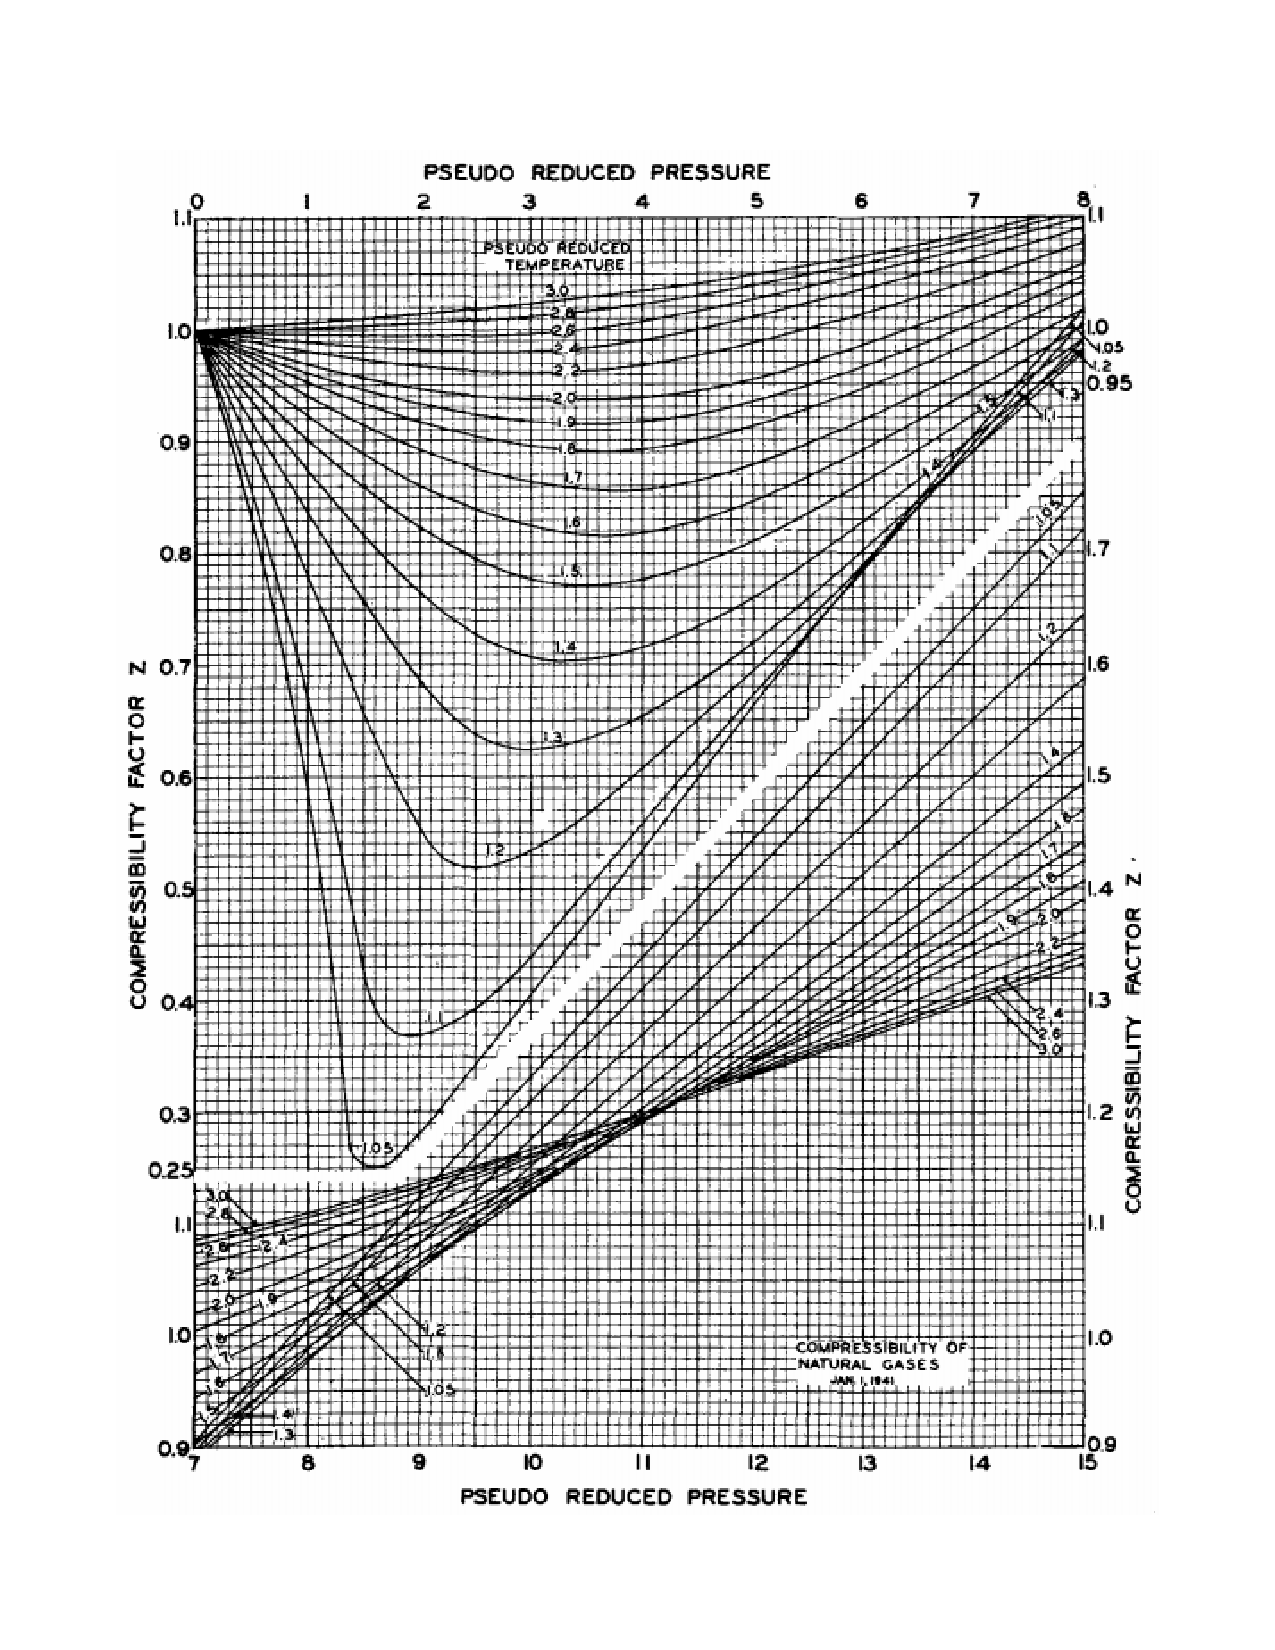
\includegraphics[width=0.70\columnwidth]{images/StandingKatzOriginal.pdf}
\caption{Standing and Katz \cite{StandingKatz1942} Natural Gas Mixture Z-Factor Chart.}
\label{fig:StandingKatzZFactors}
\end{figure}

\begin{figure}[!h]
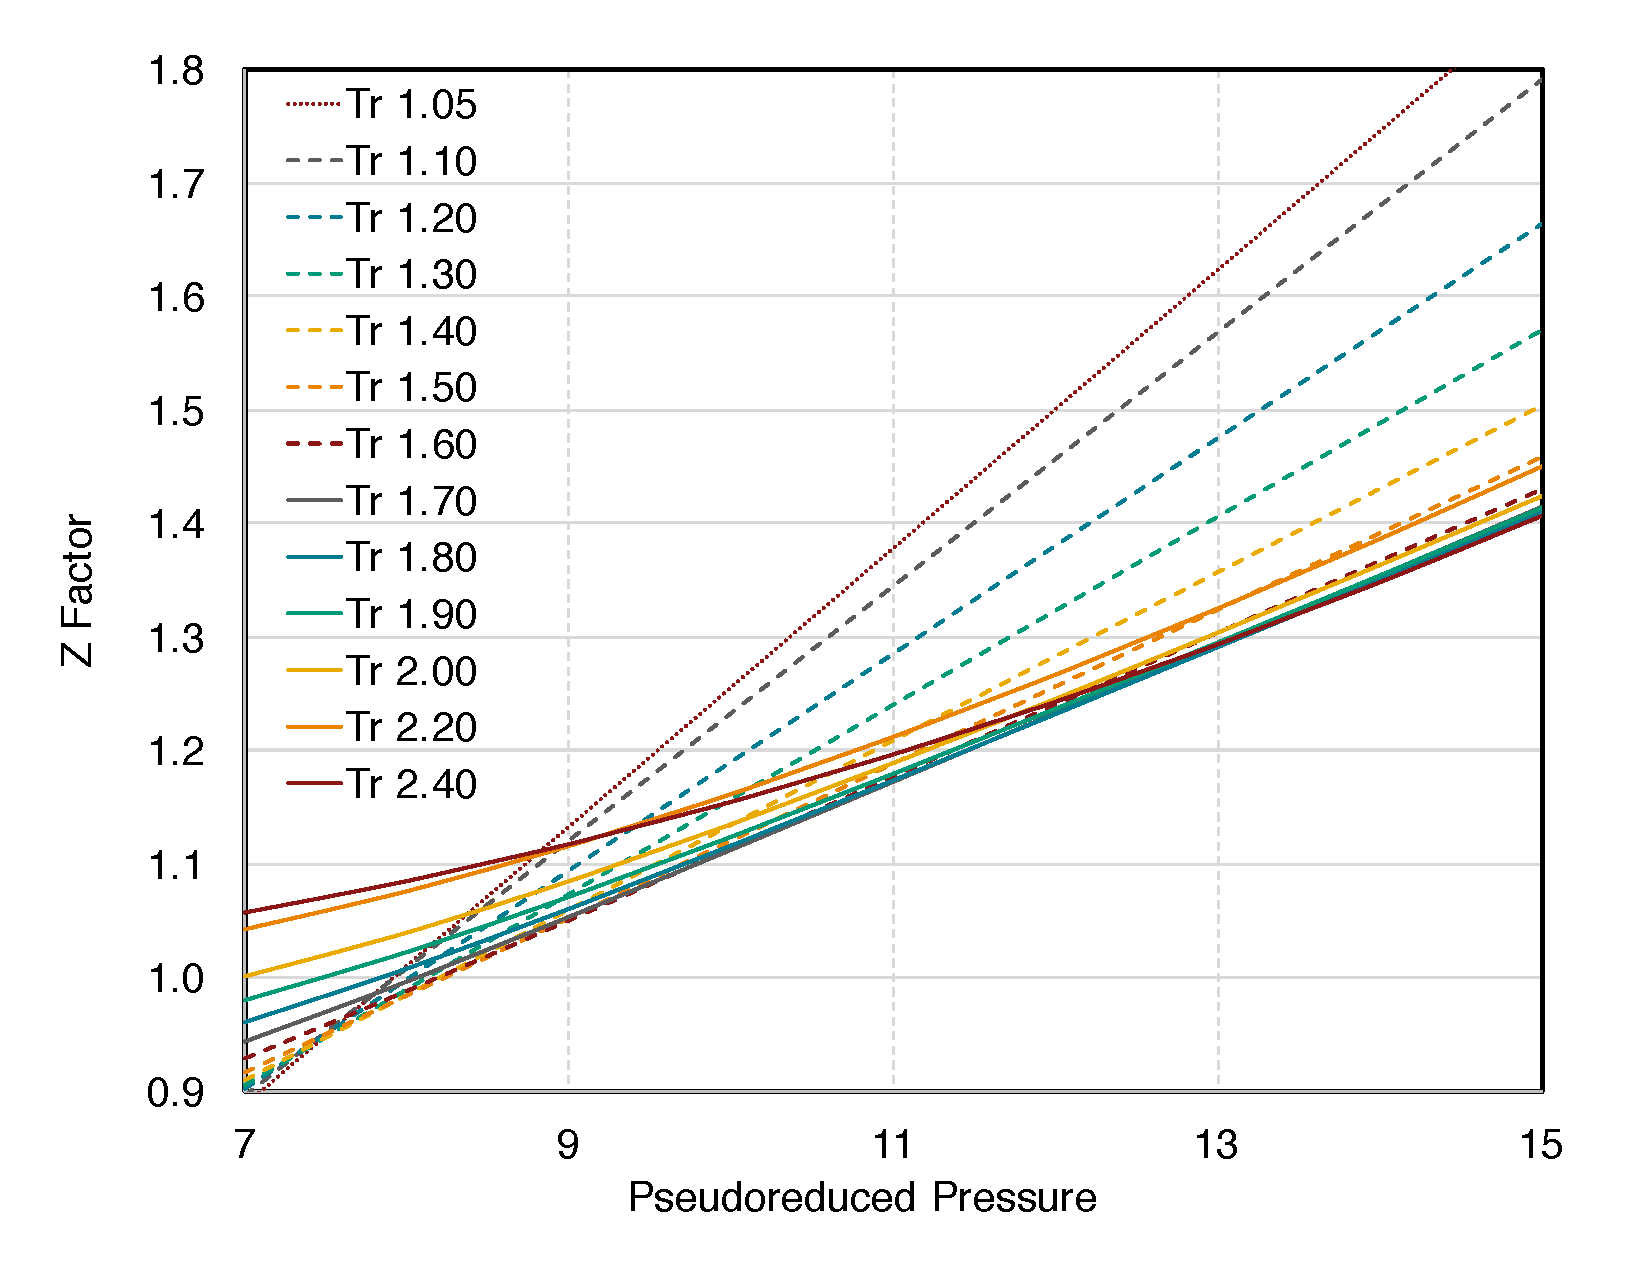
\includegraphics[width=0.70\columnwidth]{images/StandingKatzCorrelationUpper.pdf}
\caption{Correlation of Upper Portion of Standing and Katz Z-Factor Chart. Source: \cite{Standing1977}.}
\label{fig:SBBCorrelationUpper}
\end{figure}

\begin{figure}[!h]
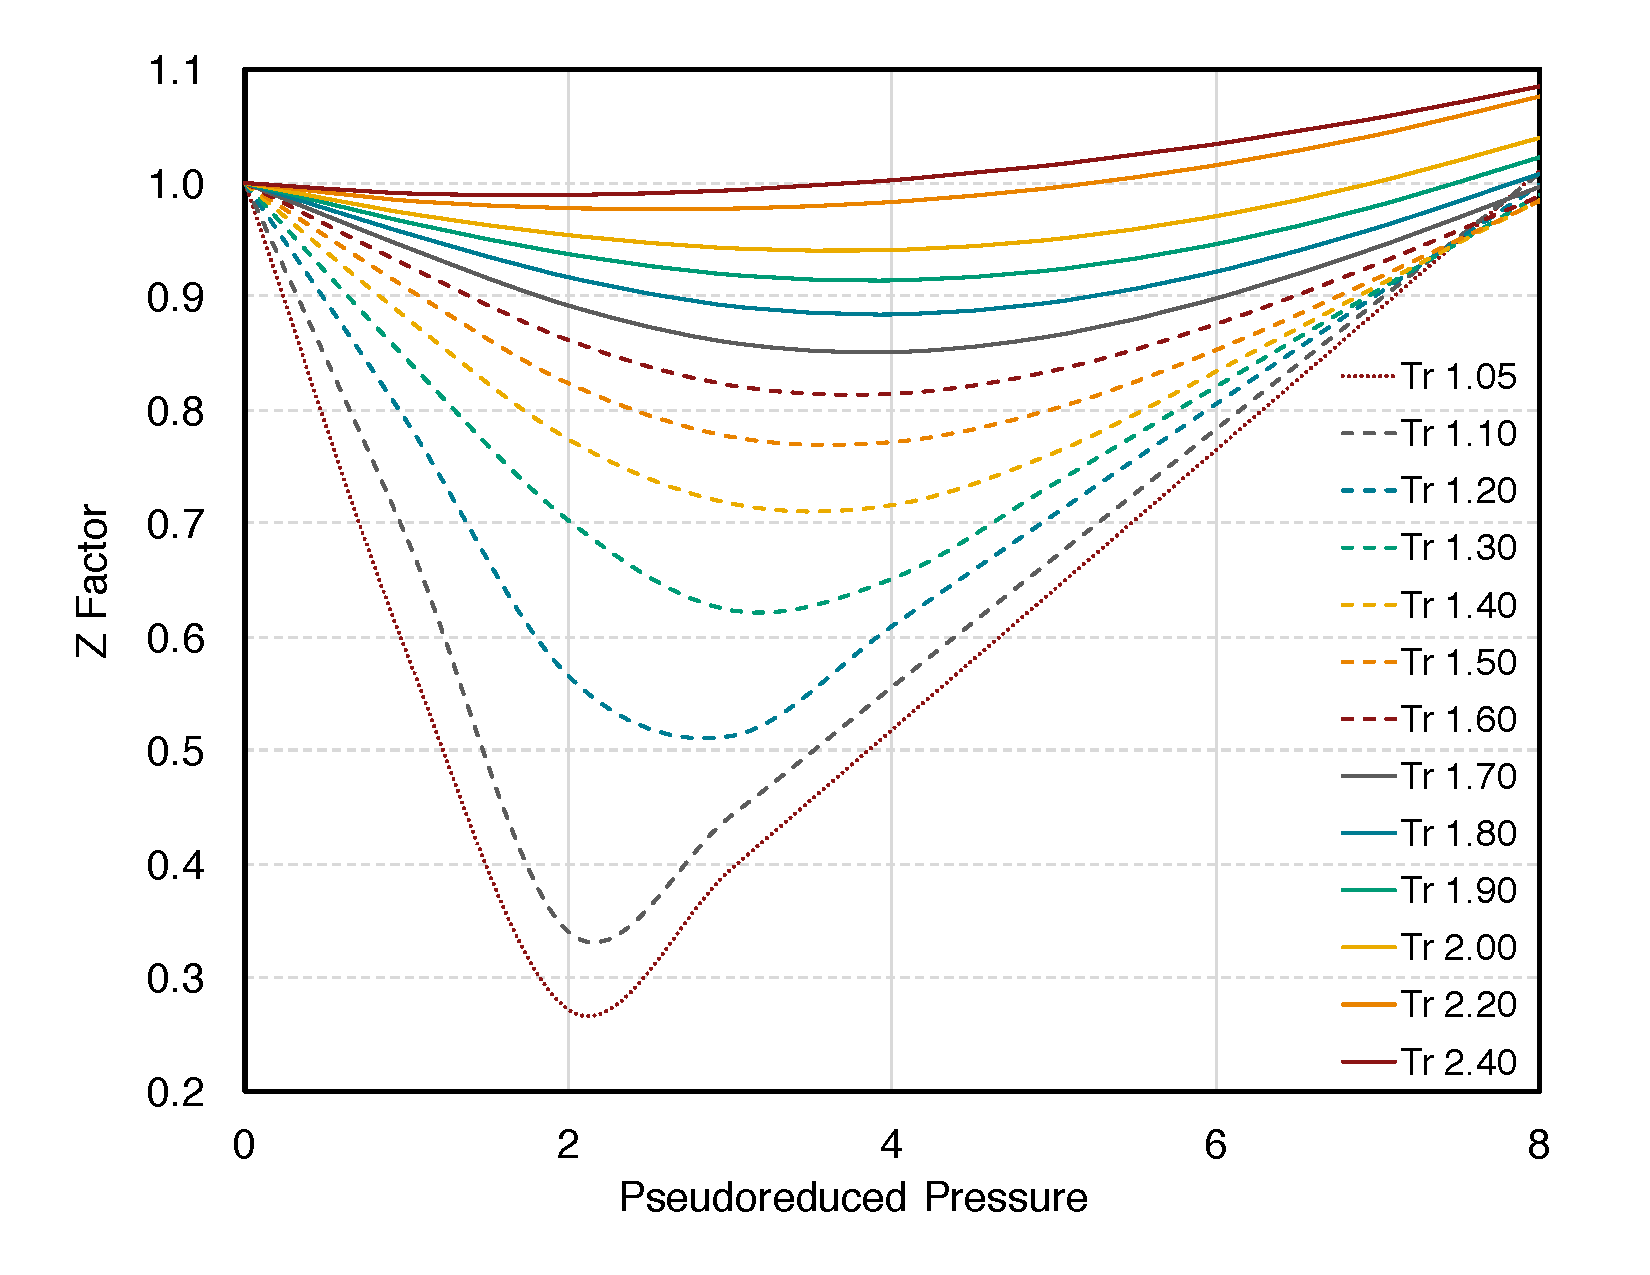
\includegraphics[width=0.70\columnwidth]{images//StandingKatzCorrelationLower.pdf}
\caption{Correlation of Lower Portion of Standing and Katz Z-Factor Chart. Source: \cite{Standing1977}.}
\label{fig:SBBCorrelationLower}
\end{figure}



\paragraph{Gas formation volume factor}

The gas formation volume factor \xlname{GVF} is the ratio of the volume of gas at the temperature and pressure of the stream in question to the volume of the same amount (moles) of gas at standard conditions.

Given the Z-factor computed above \xlname{Z\_FACTOR}, the gas volume ratio can be computed as:
\begin{equation}
FVF_g= \frac{Z p_{0} T}{p T_{0}} \eqnunitfrac{m$^3$}{std m$^3$}
\end{equation}

where $T$ is the absolute temperature of the stream [$^\circ$R], $T_0$ is the ambient absolute temperature \xlname{Amb\_temp} [$^\circ$R], $p$ is the pressure of the stream [psia] and $p_0$ is ambient pressure [psia] \xlname{Amb\_press}.

\paragraph{Gas density}

Gas density \xlname{RHO\_G} is given by the MW of gas relative to air, the density of air at standard conditions, and the gas formation volume factor:
\begin{equation}
\rho_g = \frac{\rho_{air}\gamma_g}{FVF_g}  \eqnunitfrac{tonne}{m$^3$}
\end{equation}

\paragraph{Gas molecular weight}

The molecular weight of the gas in a particular stream \xlname{MW\_G} is given by the mole-fraction-weighted molecular weight of species in the stream:
\begin{equation}
MW_g = \sum_i x_i MW_i
\end{equation} 
where $x_i$ is the mole fraction of species $i$ -- \xlname{MOL\_FRAC\_N2} $\ldots$ \xlname{MOL\_FRAC\_SO2} -- and $MW_i$ is the molecular weight of species $i$ [g/mol].

\paragraph{Gas volumetric flow rate}
The volumetric flow rate of gas per day \xlname{Q\_G} [m$^3$/d] is given by:
\begin{equation}
Q_g = \frac{m_{tot,g}}{\rho_g} 	\eqnunitfrac{m$^3$}{d}
\end{equation}


\paragraph{Gas energy density}

The energy density of the gas \xlname{LHV\_G} \xlname{LHV\_G\_lb} is given by the mass-fraction weighted energy densities of the species:
 [ADD EQUATION]
 
 \paragraph{Total gas energetic flow rate}
 
 The total gas energetic flow rate for a given stream is given by:
 \begin{equation}
 Q_{LHV,g} = m_{tot,g} LHV_g
 \end{equation}
 
 \subsection{Properties of water}
 
 \paragraph{Specific gravity of water}

The specific gravity of produced water \xlname{GAMMA\_W} at standard conditions is calculated using \cite[p. 481]{Fanchi2007}: \marginnote{Production \& Extraction 2.1.2} 
%%%%%%%%%%
\begin{equation} \label{eq:water_gravity}
\gamma _{w}=1+C _{sd} 0.695 \times 10^{-6} \eqnunit{-}
\end{equation}
%%%%%%%%%% 
where $C _{sd}$ = concentration of dissolved solids (also known as TDS) [\unitfrac{mg}{L}]. The constant 0.695 $\times$ 10$^{-6}$ has units of [L/mg].


\paragraph{Water formation volume factor}

The water formation volume factor \xlname{WVF} is assumed to be 1.0 for all streams. Because water is nearly incompressible, equations for $B_w$ nearly always produce values near 1 (i.e., 1.03), so reduce model complexity and possible requirements for iterative calculations by fixing $B_w$ to 1.0.

\paragraph{Water density}
Water density \xlname{RHO\_W} is given by the specific gravity of water and the water formation volume factor:
\begin{equation}
\rho_w = \frac{\gamma_w \rho_{w,0}}{B_w} \eqnunitfrac{tonne}{m$^3$}.
\end{equation}
where $\rho_{w,0}$ is the density of pure water [1000 kg/m$^3$]. Because we assume $B_w$ = 1 for simplicity, $\rho_w = \gamma_w \rho_{w,0}$. 

\paragraph{Water flow rate}
Water flow rate is computed from mass flow rate of water $m_w$ for a given stream and the density of water $\rho_w$ for that stream:
\begin{equation}
Q_w = \frac{m_w}{\rho_w} \eqnunitfrac{m$^3$}{d}
\end{equation}
[CHANGE FLOWS IN EXCEL TO BE Q RATHER THAN F].


%%%%%%%%%%%%%%%%%%%%%%%%%%%%%%%%%%%%%%%%%%%%%
%%%%%%%%%%%%%%%%%%%%%%%%%%%%%%%%%%%%%%%%%%%%%
%%%%%%%%%%%%%%%%%%%%%%%%%%%%%%%%%%%%%%%%%%%%%

\chapter{Gathering worksheets}

This section explains three worksheets in OPGEE which are used to collect output from intermediate calculations in process stage and supplemental worksheets. This collected output is used to calculate the overall WTR energy consumption and GHG emissions of the study crude. These gathering worksheets are the \sheet{Energy Consumption}, \sheet{GHG Emissions}, and \sheet{Active Field} worksheets. 


\clearpage

%%%%%%%%%%%%%%%%%%%%%%%%%%%%%%%%%%%%%
\section{\sheet{Energy Consumption} gathering worksheet}\label{sec:energy_consumption}

In the \sheet{Energy Consumption} gathering worksheet, energy use is summed in order of process stages, from Exploration to Waste disposal. For consistency, all energy inputs are summed on a daily basis, either as thermal energy (MMBtu/d) or as electrical energy (kWh/d). All energy types are classified using a fuel code. The primary energy types included are: 1A) Natural gas; 1B) Natural gas liquids; 2) Diesel fuel; 3) Electricity; 4) Crude oil.

First, \marginnote{Energy \\ Consumption \\ Table 1} the amount and type of fuel consumed by each process stage (e.g., Exploration, Drilling \& Development, etc) is collected using nested if then statements. Second, \marginnote{Energy \\ Consumption \\ Table 2} the fuel consumption is summed by fuel type (e.g., natural gas, diesel) to calculate the gross energy consumption. 

The gross energy consumption can include double counted energy. For example, the electricity consumed to drive a pump may be generated onsite and the energy consumed to generate that electricity would also be counted as natural gas or diesel, resulting in double counting. 

The net energy consumption is calculated by \marginnote{Energy \\ Consumption \\ Table 1} fuel type. The net energy consumption is equal to the gross energy consumption for all fuels except for electricity. The net energy consumption of electricity is calculated as:
%%%%%%%%%%%%%
\begin{equation}\label{net_elec}
E_{el,net}= E_{el,gr} - E_{el,gen} \quad\quad \footnotesize{\text{[MMBtu]}}
\end{equation}
%%%%%%%%%%%%%
where $ E_{el,net}$ = net electricity consumption [MMBtu/d]; $E_{el,gr}$ = gross electricity consumption [MMBtu/d]; and $E_{el,gen}$ = total electricity generated onsite [MMBtu/d]. The total electricity generated onsite includes electricity generated using an onsite generator or simple turbine and electricity co-generated in the steam generation system, if applicable. In other words, the net electricity consumption is equal to the electricity imported from the grid, if any.

Once the \marginnote{Energy \\ Consumption \\ Table 3} net energy consumption is calculated by fuel type the energy exports/imports are calculated by fuel type. Energy exports/imports are used to calculate indirect (offsite) energy consumption and GHG emissions by fuel type. Indirect energy consumption and GHG emissions are associated with the production and transport (production only in case of exports) of the fuel consumed directly. The exports/imports of natural gas are calculated as: 
\begin{equation}
E_{ng,exp} = E_{ng,gr} - E_{ng,fuel} + E_{ng,mu} - E_{ng,rec} \quad\quad\footnotesize{\left[\frac{\text{MMBtu}}{\text{d}}\right]}
\end{equation}
where $E_{ng,exp}$ = natural gas export/import [MMBtu/d]; $E_{ng,gr}$ = gross natural gas consumption [MMBtu/d]; $E_{ng,fuel}$ = natural gas produced as fuel after gas lifting/re-injection [MMBtu/d]; $E_{ng,mu}$ = make up natural gas for gas flooding [MMBtu/d], if applicable; and $E_{ng,rec}$ = natural gas recovered from venting and fugitives. The produced gas remaining to be used as a process fuel is equal to 0 MMBtu/d in the case of gas flooding where 100\% of produced gas is re-injected. Negative $E_{ng,exp}$ represents gas exports. Positive $E_{ng,exp}$ represents gas imports.

The exports/imports of natural gas liquid (NGL) is calculated as:
\begin{equation}
E_{ngl,exp} = E_{ngl,gr} - E_{ngl,fuel} \quad\quad\footnotesize{\left[\frac{\text{MMBtu}}{\text{d}}\right]}
\end{equation}
where $E_{ngl,exp}$ = NGL export/import [MMBtu/d]; $E_{ngl,gr}$ = gross NGL consumption [MMBtu/d]; and $E_{ngl,fuel}$ = amount of NGL produced as fuel [MMBtu/d]. 

The import of diesel is equal to gross diesel consumption. The export of diesel does not apply because diesel is not produced in upstream operations. The export/import of electricity is equal to electricity net consumption as calculated in eq.\,\eqref{net_elec}. Positive net electricity consumption is equal to electricity imported from the grid and negative net electricity consumption is equal to electricity exported to the grid. Crude oil export/import does not apply because crude oil is the main product. Any crude oil used as a process fuel on site is subtracted from the amount produced and shipped (see Section\,\ref{sec:active_field}).

Finally, \marginnote{Energy \\ Consumption \\ Table 4} the indirect energy consumption by fuel type is calculated. The indirect energy consumption is calculated as:
\begin{equation}
\begin{split}
& E_{k,ind} = E_{k,exp} \, E_{k,FC} \quad\quad \text{for}\,\, E_{k,exp} > 0\\
& E_{k,ind} = E_{k,exp} \, E_{k,DS} \quad\quad \text{for}\,\, E_{k,exp} < 0 \,\,\text{and displacement}\\
& E_{k,ind} = 0 \quad\quad\quad\quad\quad\quad\,\, \text{for}\,\, E_{k,exp} < 0 \,\,\text{and allocation by energy value}\\
\end{split}
\end{equation}
where $k$ refers to the fuel type; $E_{k,ind}$ = indirect energy consumption [MMBtu/d]; $E_{k,exp}$ = fuel export/import [MMBtu/d]; $E_{k,FC}$ = fuel cycle energy consumption [MMBtu/MMBtu]; and $E_{k,DS}$ = energy consumption of displaced system in case of fuel export [MMBtu/MMBtu]. For details on the energy consumption of fuel cycles and displaced systems, see Section \ref{sec:fuel_cycle}.


\clearpage

%%%%%%%%%%%%%%%%%%%%%%%%%%%%%%%%%%%%%
\section{\sheet{GHG Emissions} gathering worksheet}\label{sec:GHG_emissions}

The GHG emissions gathering worksheet compiles and computes emissions of all emissions types across all process stages. The first step \marginnote{GHG \\ Emissions Table 1}is the calculation of direct GHG emissions from the different components of the model. Direct GHG emissions are calculated as: 
%%%%%%%%%%%%
\begin{equation}
EM_{s,k} = E_{s,k,gr} \, EF_{s,k} \quad\quad\footnotesize{\left[\frac{\text{gCO$_{2}$eq}}{\text{d}}\right]} \label{direct_emissions}
\end{equation}
%%%%%%%%%%%%
where $s$ = emissions source (e.g., downhole pump driver); $k$ = fuel type;\newline $EM_{s,k}$ = direct GHG emissions from the consumption of fuel $k$ in source $s$ [gCO$_{2}$eq/d]; and $E_{s,k,gr}$ = gross energy consumption of fuel $k$ in source $s$ [MMBtu/d]; and $EF_{s,k}$ = emissions factor of source $s$ using fuel $k$ [g CO$_2$ eq./MMBtu]. This equation does not apply to electricity, where direct GHG emissions are equal to 0 gCO$_{2}$eq./d.

Next, \marginnote{GHG \\ Emissions Table 1} the GHG emissions from land use, flaring, and venting/fugitives are calculated by process stage. This includes gathering emissions calculated in each process stage and supplemental worksheets.

The next step \marginnote{GHG \\ Emissions Table 2} is the calculation of indirect GHG emissions by fuel import type. The indirect GHG emissions are calculated as:
\begin{equation}
\begin{split}
& EM_{k,ind} = E_{k,exp} \, EM_{k,FC} \quad\quad \text{for}\,\, E_{k,exp} > 0\\
& EM_{k,ind} = E_{k,exp} \, EM_{k,DS} \quad\quad \text{for}\,\, E_{k,exp} < 0 \,\,\text{and displacement}\\
& EM_{k,ind} = 0 \quad\quad\quad\quad\quad\quad \text{for}\,\, E_{k,exp} < 0 \,\,\text{and allocation by energy value}\\
\end{split}
\end{equation} 
where $k$ refers to the fuel type; $EM_{k,ind}$ = indirect GHG emissions from fuel consumption [gCO$_{2}$eq/d]; $E_{k,exp}$ = fuel export/import [MMBtu/d]; $EM_{k,FC}$ = fuel cycle GHG emissions [gCO$_{2}$eq/MMBtu]; and $EM_{k,DS}$ = GHG emissions from displaced system in case of fuel export [gCO$_{2}$eq/MMBtu]. For details on the GHG emissions of fuel cycles and displaced systems, see section \ref{sec:fuel_cycle}.

Finally, the GHG emissions gathering worksheet considers the impact \marginnote{GHG \\ Emissions Table 3} of CO$_2$ sequestration. Sequestration-related calculations are applicable only if gas flooding is selected as a production practice and CO$_2$ is selected as the flood gas. Table 3 is an overview of system-level calculations related to CO$_2$ sequestration. 

The CO$_2$ sequestration credited to the oilfield is included in the overall calculations in the \sheet{Results} worksheet. It is calculated by first considering the source of the CO$_2$. \marginnote{Active Field 2.4.7.2} If the CO$_2$ was acquired from a naturally occurring subterranean source then no sequestration credit accrues because this CO$_2$ was already sequestered. A sequestration credit is applicable only if the CO$_2$ originated from an anthropogenic source --- it must have been captured during industrial process such as coal combustion. 

Furthermore, depending on the specific regulations and laws governing CO$_2$ sequestration, the credit may accrue either to the CO$_2$ capturing facility or to the oilfield operator injecting it into a reservoir. OPGEE also deducts CO$_2$ that is released due to long-term reservoir leakage and an oilfield operator's decision to conduct terminal phase blow-down operations. OPGEE's consideration of long-term leakage and operator blow-down is described in Section \ref{sec:Sequestration}\marginnote{Production \& Extraction 1.2.9.2, 1.2.9.3}.

If the carbon dioxide used for EOR is anthropogenic, then the overall CO$_2$ sequestration credit accruing to the oilfield is calculated as:
%%%%%%%%%%
\begin{equation} \label{eq:SequestrationCredit}
CR_{CO_{2}} = P_{oilfield} \cdot (Seq_{CO_{2}} - Blow_{CO_{2}} - Leakage_{CO_{2}}) \quad \quad \begin{footnotesize}\left[ \frac{\text{gCO$_2$}}{\text{d}} \right] \end{footnotesize}
\end{equation}
%%%%%%%%%%
 where $CR_{CO_{2}}$ = CO$_2$ sequestration credit assigned to the oilfield [gCO$_2$/d]; $P_{oilfield}$ = proportion of the overall sequestration credit assigned to the oilfield [-]; $Seq_{CO_{2}}$ = CO$_2$ sequestration rate [gCO$_2$/d]; $Blow_{CO_{2}}$ = CO$_2$ lost from the reservoir from terminal blow-down operations [gCO$_2$/d]; and $Leakage_{CO_{2}}$ = the amount of CO$_2$ leaving the reservoir from long-term leakage [gCO$_2$/d].




%%%%%%%%%%%%%%%%%%%%%%%%%%%%%%%%%%%%%%%%%%%%%
%%%%%%%%%%%%%%%%%%%%%%%%%%%%%%%%%%%%%%%%%%%%%
%%%%%%%%%%%%%%%%%%%%%%%%%%%%%%%%%%%%%%%%%%%%%

\chapter{Process worksheets}

This section explains the main assumptions and calculations for each process worksheet. Items discussed include user assumptions and choices, process calculation assumptions, calculations of input parameters, and calculations of intermediate outputs.


\clearpage
%%%%%%%%%%%%%%%%%%%%%%%%%%%%%%%%%%%%%%%%%%%%%
\section{Exploration}\label{sec:exploration}

Emissions from petroleum exploration occur during clearing of land for seismic surveys, operation of seismic survey equipment, drilling of exploratory wells, and from fugitive emissions during drilling operations. Offsite emissions occur due to other materials and services consumed during drilling (e.g., computing energy consumed during seismic data processing). A complete list of emissions sources, along with their categorization and estimated magnitude, is shown in Table \ref{tab:exploration_sources}.

Required inputs for exploration emissions include the following terms gathered from the \sheet{Active Field} worksheet:\marginnote{Exploration 1.1}
\begin{itemize}
\item Field depth [ft]
\item Is field offshore [0-1]
\item Field production rate [bbl/d]
\end{itemize}

Required inputs to be entered for secondary interaction on the \sheet{Exploration Emissions} worksheet include:\marginnote{Exploration 1.2.1 - 1.2.5}
\begin{itemize}
\item Distance of travel for survey
\item Weight of land survey vehicle
\item Weight of ocean survey vehicle
\item Dry holes drilled per field found
\item Exploratory or scientific wells drilled after field discovery (non-producing)
\end{itemize}
The default values for these inputs are noted in Table \ref{tab:exploration}.

\subsection{Calculations for petroleum exploration}

The survey vehicle energy consumption (e.g., seismic survey ship or seismic survey trucks) are calculated as:
%%%%%%%%%%%%%%%%
\begin{equation}\label{eq:trans_Etr}
\begin{split}
& E_{EXP} = \sum_{j} y_j m_j D_{j} UE_{j} \quad\quad (j \in S,T) \\
& \begin{footnotesize} \left[ \text{mmBtu} \right] =\left[- \right]  \left[\text{ton} \right]  \left[ \text{mi} \right] \left[ \frac{\text{Btu}}{\text{ton-mi}} \right] 
\end{footnotesize}
\end{split}
\end{equation}
%%%%%%%%%%%%%%%%
where $y_j$ is a binary variable representing whether exploration mode $S$ (ship-based exploration) or $T$ (truck-based exploration) is performed [-]; $m_j$ is the weight of exploration vehicle $j$ [ton], $D_j$ is the distance traveled by exploration vehicle $j$ [mi], and $UE_{j}$ is the energy-specific effectiveness of transport type $j$ [Btu/ton-mi], as computed on the \sheet{Transport} worksheet.\marginnote{Transport 2.2}

Energy consumed in drilling exploratory wells is computed using drilling energy intensity computed on the \sheet{Drilling \& Development} sheet.

Energy consumed in exploration is computed as a fraction of the total lifetime energy production assumed produced from the field.  This quantity is derived in the \sheet{Drilling \& Development} sheet, as described below.



\subsection{Defaults for petroleum exploration}

Table \ref{tab:exploration} shows the default settings for petroleum exploration.


\begin{landscape}
\begin{table}
\begin{scriptsize}
\tablefirsthead{\toprule Param. & Description & Eq. no. & Default & Literature range & Unit & Sources & Notes\\
\midrule}
\tablehead{ \multicolumn{5}{p{1\columnwidth}}{\textit{Continued from previous page}}\\ \toprule Param. &Description & Eq. no. &Default & Literature range & Unit & Sources & Notes \\ 
\midrule }
\tabletail{\bottomrule \multicolumn{5}{p{1\columnwidth}}{\textit{Continued on next page...}}\\}
\tablelasttail{\bottomrule}
\tablecaption{Default inputs for exploration emissions}
\label{tab:exploration}
\begin{threeparttable}
\begin{supertabular*}{1\columnwidth}{p{0.05\columnwidth}p{0.4\columnwidth}p{0.05\columnwidth}p{0.05\columnwidth}p{0.07\columnwidth}p{0.1\columnwidth}p{0.05\columnwidth}p{0.05\columnwidth}}
$D_{j} $ & Distance exploration mode $j$ travels  (same for $S$ and $T$)	& - 	& 10,000& - &[mi] & & a\\ 
$m_{S} $ & Weight of exploration ship 	& - 	& 100 & - &[ton] & & b\\ 
$m_{T}$ & Weight of exploration truck 	& - 	& 25  & - & [ton] & & c \\
$UE_{S}$ & Effectiveness of exploration ship 	& - & 27 	& & [Btu/ton-mi] & \cite{Wang2009}&  \\
$UE_{T}$ & Effectiveness of exploration truck 	& - & 969 	& & [Btu/ton-mi] & \cite{Wang2009}&  \\
\end{supertabular*}
\begin{tablenotes}
\item[a] Simple assumption for distance of travel to remote exploration site. Distance traveled during actual survey is assumed by default to be small compared to distance to field location.
\item[b] Simple assumption for weight of exploration ship
\item[c] Simple assumption for weight of exploration truck
\end{tablenotes}
\end{threeparttable}
\end{scriptsize}
\end{table}


\end{landscape}



%%%%%%%%%%%%%%%%%%%%%%%%%%%%%%%%%%%%%%%%%%%%%%%%
\clearpage
\section{Drilling \& development}\label{sec:drilling}

\subsection{Introduction to drilling \& development}

Drilling and development operations result in a variety of emissions. Well drilling and installation of production equipment results in on-site energy use (e.g., for rigs and other construction equipment) as well as indirect offsite energy use (e.g., embodied energy consumed to manufacture well casing). Drilling and development also results in land use impacts, which can release biogenic carbon from disturbed ecosystems and soils \cite{Yeh2010}. In addition, fugitive emissions can occur during the drilling process. A list of emissions sources, along with their categorization and estimated magnitude, is shown in Table \ref{tab:drilling_sources}.


\subsection{Calculations for drilling \& development}

Three aspects of field drilling and development are modeled in OPGEE \version: drilling energy consumption, hydraulic fracturing energy consumption, and land use impacts. \marginnote{Active Field 3.8} Other emissions from drilling and development are not explicitly modeled and therefore would be accounted for in the small sources term. The parameters and variables used in the drilling and development model equations are listed in Table \ref{tab:defaults_drilling}. 

\subsubsection{Emissions from drilling}

Drilling oil wells consumes fuel. This fuel is consumed on site in prime movers (generally diesel engines) for a variety of purposes: to power mud pumps; apply torque to drill string; pull drill string; raise, lower and retrieve subsurface monitoring equipment; and pump cement. 

Relationships for these functions are derived from the open-source drilling energy intensity model \emph{GHGfrack} \cite{Vafi2016a, Vafi2016b, Vafi2016c}. The GHGfrack model is developed with extensive documentation and validation efforts \cite{Vafi2016a, Vafi2016b}.  

In order to develop correlations for use in OPGEE \version, we ran a number of cases in GHGfrack.  First, three well complexity settings are designed in GHGfrack (see Figure \ref{fig:hole_diam}).  These well complexity designs are also used in the \sheet{Embodied Emissions} worksheet, as described below.  \marginnote{Drilling \& Development 1.2}The \emph{Simple} well design has one string of surface casing and one string of production casing.  The \emph{Moderate} well design has one string of surface casing, one string of intermediate casing, and one string of production casing.  The \emph{Complex} well design has one string of surface casing, two strings of intermediate casing, and one string of production casing.  These wellbore designs are derived from examples in industry texts \cite{Mitchell2006}. For each casing design an appropriate set of true vertical depth (TVD) values is chosen based on well complexity. \emph{Simple} wells are assumed to range between 0 ft and 12,000 ft deep, \emph{Moderate} wells are between 4,000 and 16,000 feet deep, while \emph{Complex} wells are between 12,000 and 20,000 feet deep.  Each TVD is incremented in segments of 1000 ft.  

Each well casing design plan is designed for four wellbore diameters, called \emph{Small}, \emph{Medium}, \emph{Large} and \emph{Extra-large}.  The diameters (hole diameter not casing diameter) for each of these cases is listed for each well complexity in Table \ref{tab:drilling_diam}.  These hole diameters are chosen from API casing-hole size charts \cite[Figure 11.22]{Mitchell2006}.   The resulting depth ranges for each casing string section are given in Table \ref{tab:drilling_length}.  

\begin{landscape}
\begin{table}
\begin{scriptsize}
\tablefirsthead{\toprule String & Simple &        &        &   & Moderate &        &        &   & Complex &        &        &   \\
\midrule
 & Small  & Med    & Large  & Extra-large & Small    & Med    & Large  & Extra-large & Small   & Med    & Large  & Extra-large \\
\midrule}
\tablehead{ \multicolumn{5}{p{1\columnwidth}}{\textit{Continued from previous page}}\\ \toprule Param. &Description & Eq. no. &Default & Literature range & Unit & Sources & Notes \\ 
\midrule }
\tabletail{\bottomrule \multicolumn{5}{p{1\columnwidth}}{\textit{Continued on next page...}}\\}
\tablelasttail{\bottomrule}
\tablecaption{Hole diameters for different casing sections under three wellbore designs (in.)}
\label{tab:drilling_diam}
\begin{threeparttable}
\begin{supertabular*}{1\columnwidth}{p{0.1\columnwidth}|p{0.05\columnwidth}p{0.05\columnwidth}p{0.05\columnwidth}p{0.05\columnwidth}|p{0.05\columnwidth}p{0.05\columnwidth}p{0.05\columnwidth}p{0.05\columnwidth}|p{0.05\columnwidth}p{0.05\columnwidth}p{0.05\columnwidth}p{0.05\columnwidth}}
Conductor 	& -      & -      & -      & - & -        & -      & -      & - & -       & -      & -      & - \\
Surface 		&12.250 & 12.250 & 14.750 & 14.750      & 12.250   & 14.750 & 14.750 & 14.750      & 17.500  & 14.375 & 17.500 & 17.500      \\
Intermediate 1 	&5.875  & 6.125  & 6.500  & 7.875       & 8.750    & 10.625 & 10.625 & 12.250      & 14.750  & 10.625 & 12.250 & 14.750      \\
Intermediate 2 	&5.875  & 6.125  & 6.500  & 7.875       & 5.875    & 5.875  & 6.125  & 7.875       & 12.250  & 7.875  & 9.500  & 12.250      \\
Production 	&5.875  & 6.125  & 6.500  & 7.875       & 5.875    & 5.875  & 6.125  & 7.875       & 9.500   & 6.500  & 7.875  & 9.500      \\
\end{supertabular*}
\end{threeparttable}
\end{scriptsize}
\end{table}

\begin{table}
\begin{scriptsize}
\tablefirsthead{\toprule String  & Simple & Moderate & Complex        \\
\midrule}
\tablehead{\toprule String  & Simple & Moderate & Complex        \\
\midrule}
\tabletail{}
\tablelasttail{\bottomrule}
\tablecaption{Bottomhole depth for different segments (ft.)}
\label{tab:drilling_length}
\begin{threeparttable}
\begin{supertabular*}{0.6\columnwidth}{p{0.12\columnwidth}p{0.12\columnwidth}p{0.12\columnwidth}p{0.12\columnwidth}}
Conductor 	& 50      			& 50      			& 50      		  	\\
Surface 		&250 - 2,000		& 1,000 - 2,000 		& 2,000 		  	\\
Intermediate 1 	& -  				& 2,000 - 4,000  		& 6,000       		\\
Intermediate 2 	& -  				& -  				& 9,000-12,000  	 \\
Production 	& 1,000 - 12,000 	& 4000 - 16,000  	& 12,000-20,000        \\
\end{supertabular*}
\end{threeparttable}
\end{scriptsize}
\end{table}

\end{landscape}


\begin{figure}[t]
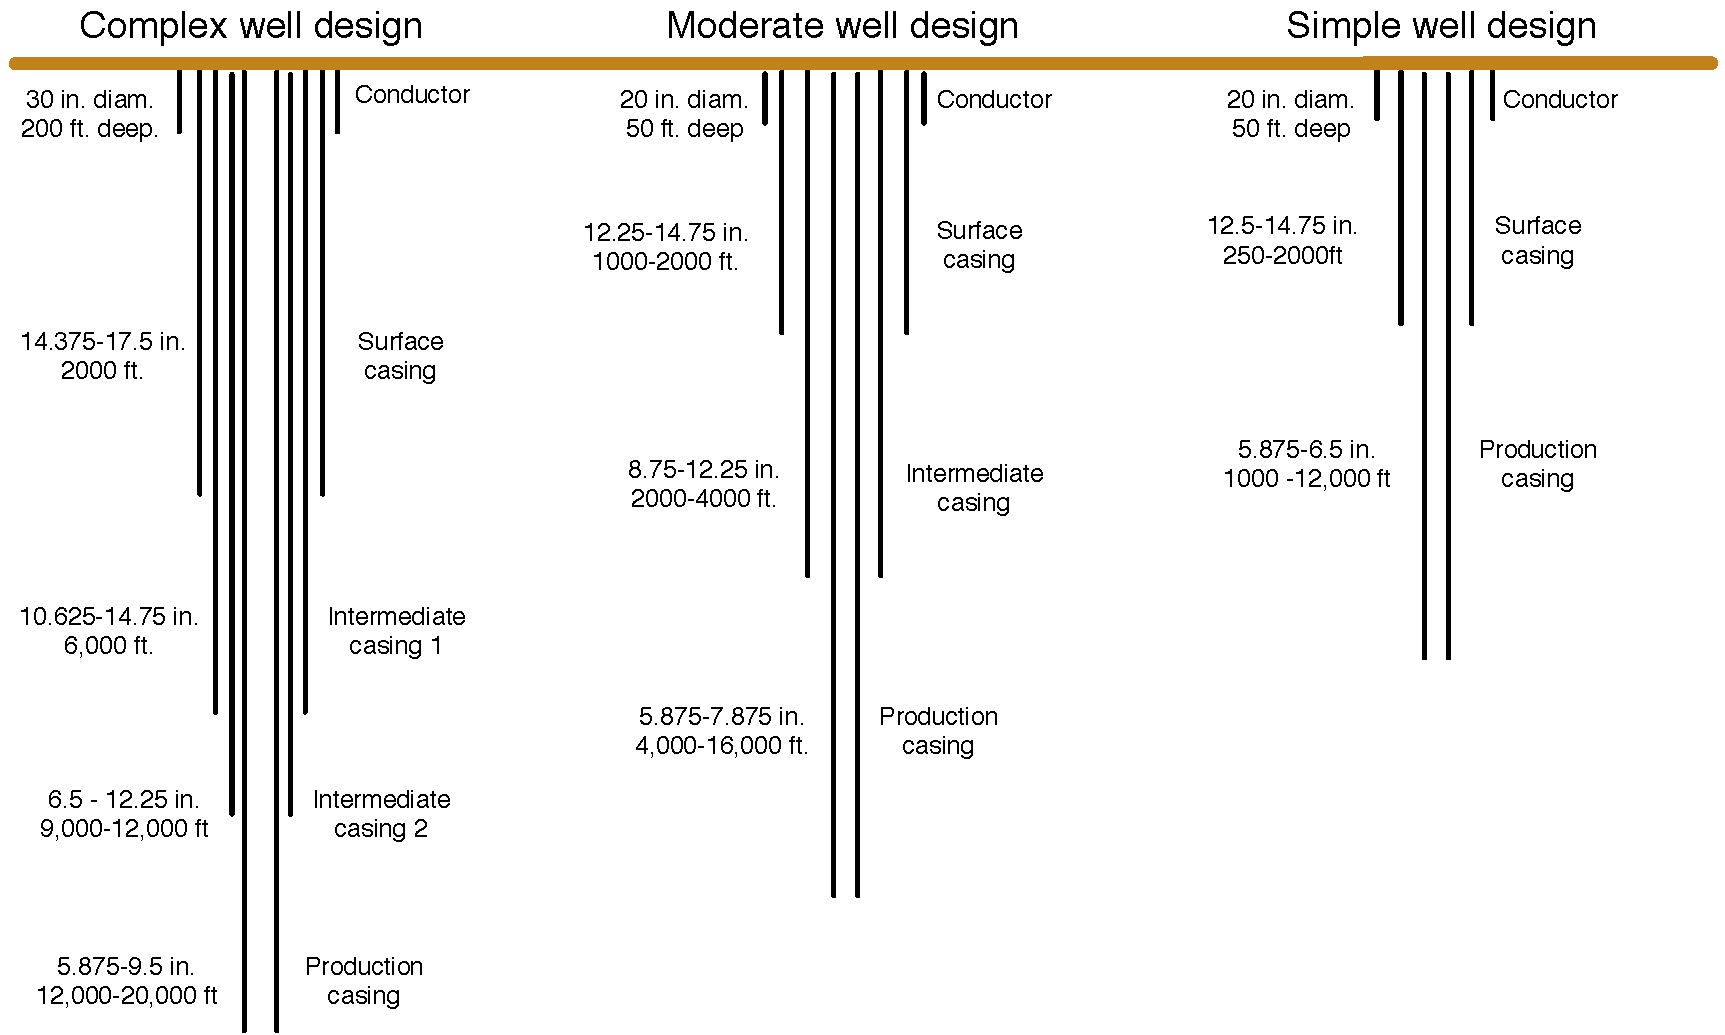
\includegraphics[width=1\columnwidth]{images/all_well_hole_diam.pdf}
\caption{Drilling hole diameters for simple, moderate and complex well construction.}
\label{fig:hole_diam}
\end{figure}

In addition, the energy efficiencies of rotary table/drill string torque provision and mud pump work are varied. The moderate efficiency settings for these terms are 45\% and 65\% respectively \cite{Vafi2016b}.  The low and high efficiency settings are 40\% and 50\% for the rotary table and 60\% and 70\% for the mud pumps, respectively.

The resulting energy consumption for rotary table and mud circulation uses are therefore modeled as:
\begin{equation}
E_{D} = E_{D}^{rt} + E_{D}^{mp}
\end{equation}
Where $E_{D}^{rt}$ is the energy consumed in rotary table work provision and $E_{D}^{mp}$ is the energy consumed in mud circulation pumps.

The energy consumption for rotary table work $E_{D}^{rt}$ is computed using the torque and torque factors as noted in GHGfrack documentation \cite{Vafi2016b}:
\begin{equation}
E_{D}^{rt} = BHP^{rt} \times t,
\end{equation}
or,
\begin{equation}
E_{D}^{rt} = \frac{2 \pi T N}{33,000 \eta} \times t,
\end{equation}
where $BHP^{rt}$, is the brake horsepower required by the rotary table [hp], and $t$ is the amount of time that the rotary table is operating [h]. $BHP$ is computed using the torque $T$ [ft-lb$_f$], rotational speed $N$ [rpm], and overall electro-mechanical efficiency of the rotary table drive system $\eta$ [-]. The value 33,000 is a unit conversion factor.  These values are set equal to \emph{GHGfrack} defaults in all results presented below. If the user wishes to change torque or other rotary table inputs, please use the \emph{GHGfrack} model directly. 

The energy consumption for mud circulation is computed using the overall pressure drop in the mud circulation system \cite{Vafi2016b}:
\begin{equation}
E_{D}^{mp} = BHP^{mp} \times t,
\end{equation}
or,
\begin{equation}
E_{D}^{mp} = \frac{\Delta P_{mp} Q}{1714 \eta} \times t,
\end{equation}
where $\Delta P_{mp}$ is the pressure drop that must be overcome by the mud pump [psi], $Q$ is the mud flowrate [gal. per min.], $t$ is the time of mud pump operation [h] and 1714 is a conversion factor.

This pressure drop $\Delta P_{mp}$ is made up of a series of terms, including:
\begin{equation}
\Delta P_{mp} = \Delta P_{fric} + \Delta P_{dynamic} + \Delta P_{dm} - \Delta P_{hydrostatic} + \Delta P_{other}
\end{equation}
where subscripts refer to different pressure drop terms.  The $fric$ pressure drop is due to friction in drill string and annulus, modeled using a set of laminar and turbulent pipe and annulus flow models using different assumptions regarding non-Newtonian nature of drilling fluids (see \emph{GHGfrack} documentation \cite{Vafi2016a, Vafi2016b}).  The $dm$ term cooresponds to energy imparted on the mud motor and converted to rotational motion of the bit.  In developing results for OPGEE, all \emph{GHGfrack} mud circulation settings are left at \emph{GHGfrack} defaults. If the user wishes to mud circulation inputs, please use the \emph{GHGfrack} model directly. 

Given overall energy term $E_{D}$, we can compute fuel use in drilling as follows:
\begin{equation}
F_{D} = \frac{E_{D} \eta_{gs}}{LHV_{di}}
\end{equation}
where $F_{DD}$ is the fuel use in drilling and development [gal], $\eta_{gs}$ is the efficiency of the drilling prime mover (diesel engine) [-], and $LHV_{di}$ is the lower heating value of diesel fuel [mmBtu/gal].

A number of other \emph{GHGfrack} settings are required. For simplicity, in each model run, the drill pipe outer diameter (OD) [in] is set equal to 2.5 in. smaller than the smallest casing string inner diameter (ID).  In all cases, the drill pipe ID is set equal 0.5 in. smaller than the drill pipe OD.  The drill collar OD is set equal to 1.5 in. smaller than the smallest casing string ID.  The drill collar ID is set equal 0.5 in. smaller than the drill collar OD.  Also, in each well design, the last segment is set to an inclination angle of either 0$^\circ$ (vertical) or 90$^\circ$ (horizontal).  We do not apply a slanted transition zone (i.e., a 45 $^\circ$ zone).   

Given all of the above variables, a total of 816 \emph{GHGfrack} model runs are computed using an automated macro.  The resulting depths and fuel consumption quantities for all runs are illustrated in Figure \ref{fig:drilling1}.  

\begin{figure}[tb]
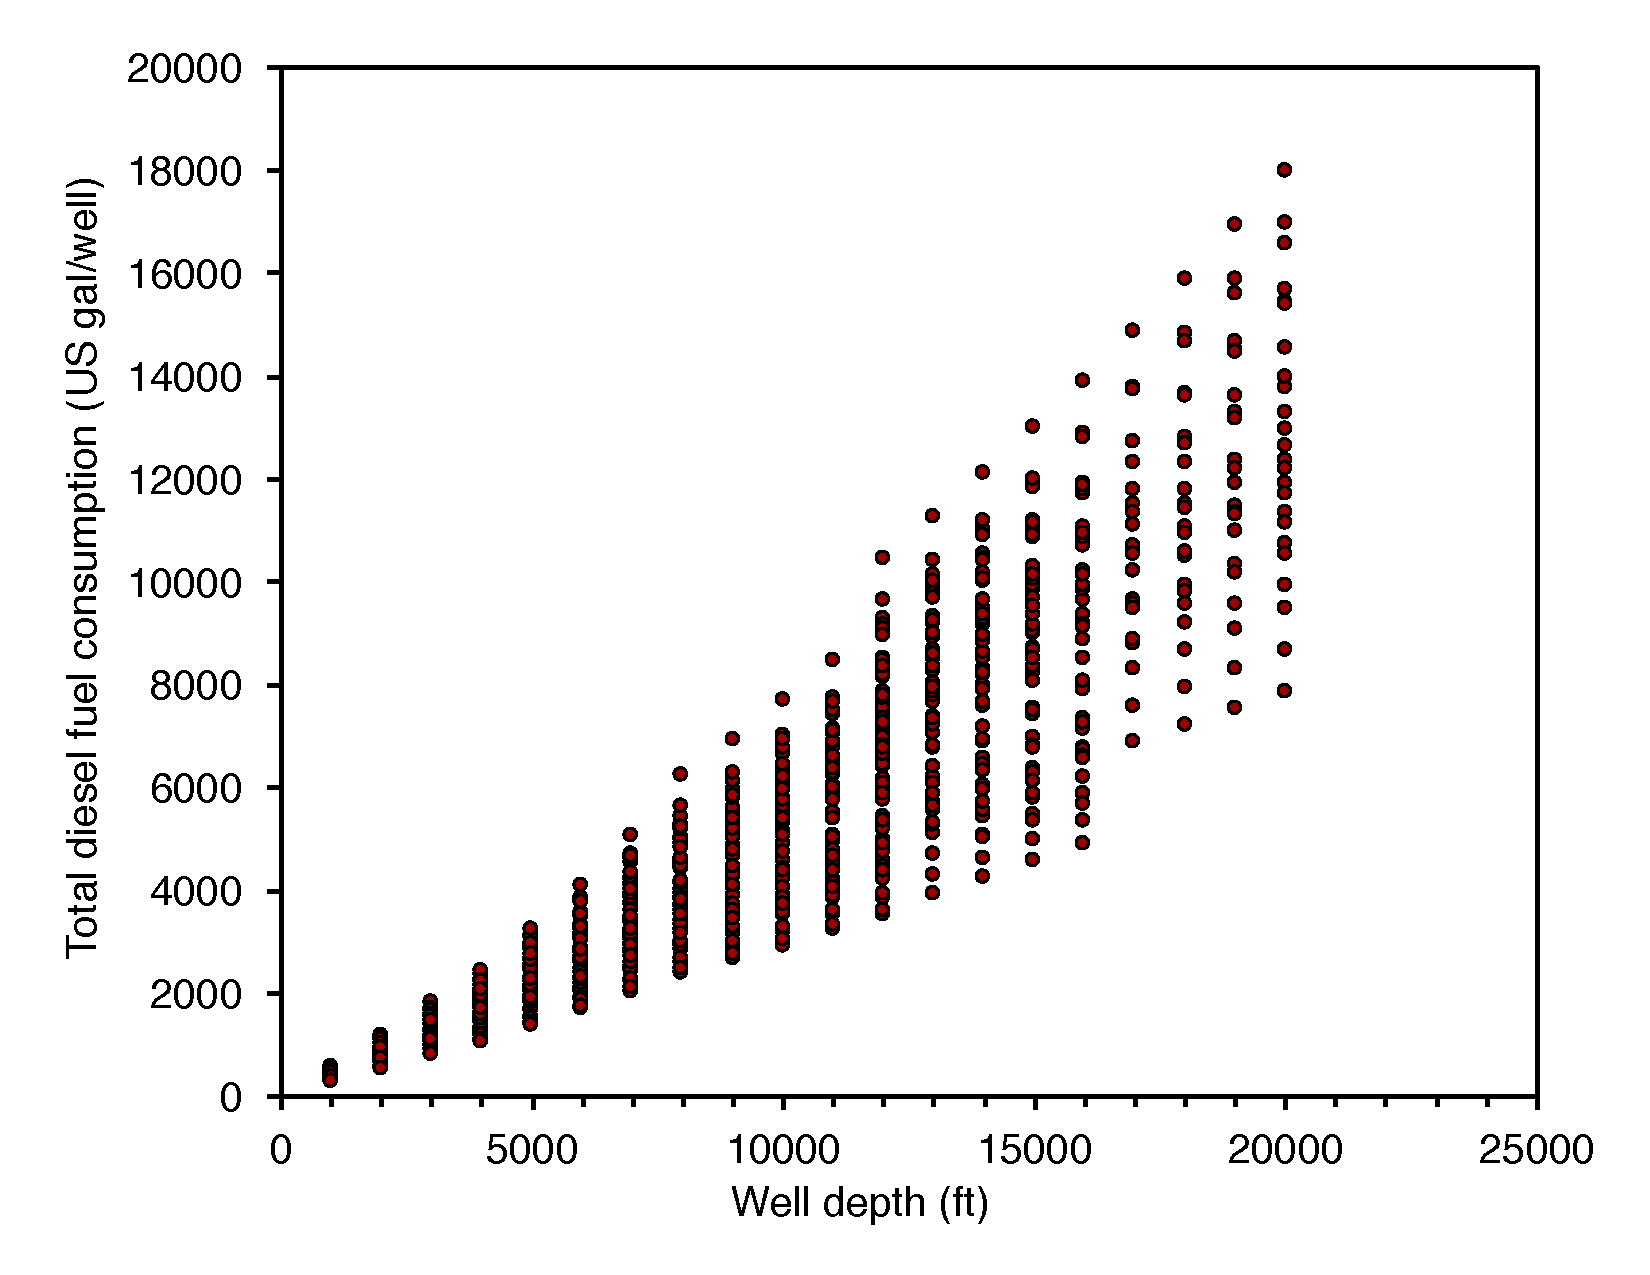
\includegraphics[width=0.8\columnwidth]{images/Drilling1.pdf}
\caption{All GHGfrack results for drilling fuel consumption in US gallons of diesel (includes both rotary table + mud circulation).}
\label{fig:drilling1}
\end{figure}

As can be seen, there is a wide range of energy consumption values for each depth.  To further understand drivers of emissions, we then segment these results into results from simple, moderate, and complex wells (Figure \ref{fig:drilling2}).

\begin{figure}[tb]
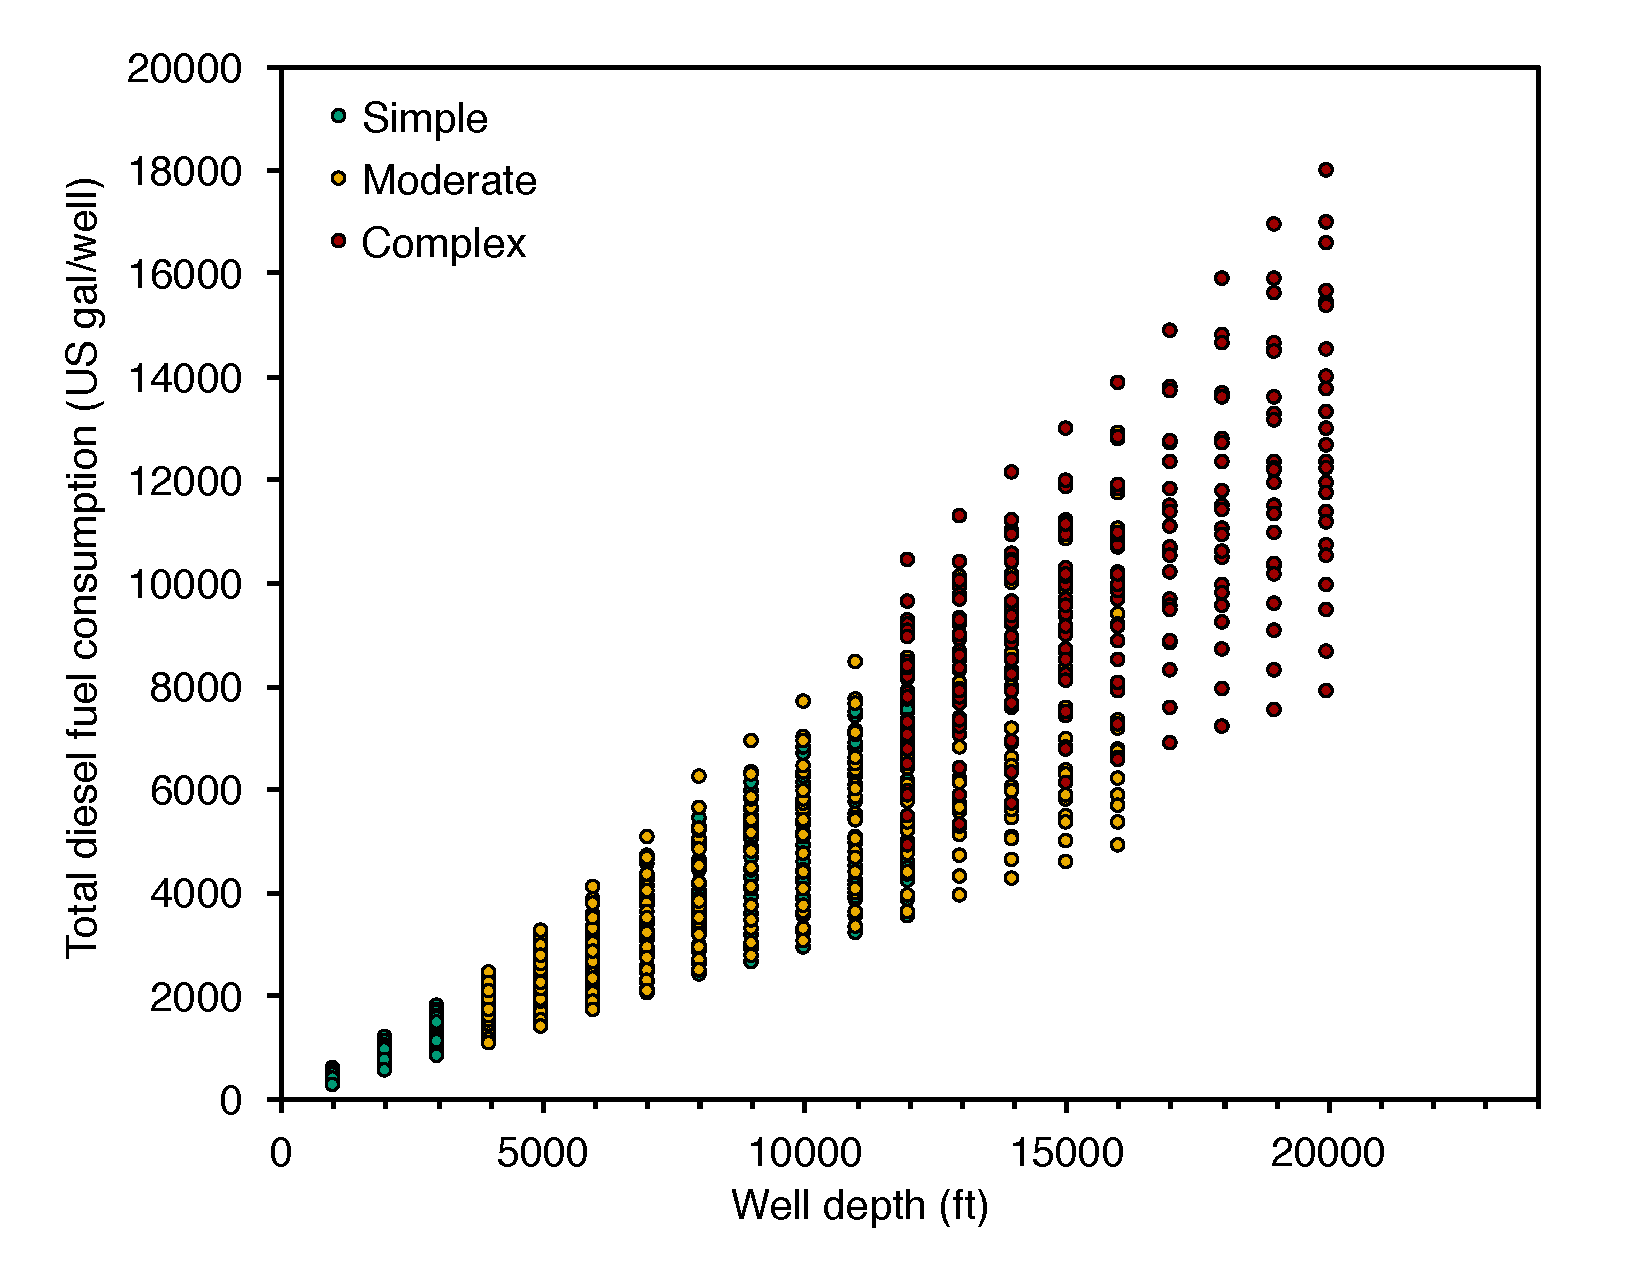
\includegraphics[width=0.8\columnwidth]{images/Drilling2.pdf}
\caption{GHGfrack results for drilling fuel consumption segmented by well complexity. Fuel consumption reported in US gallons of diesel (includes both rotary table + mud circulation).}
\label{fig:drilling2}
\end{figure}

We can further segment these results by separating vertical and horizontal wells and by noting the effect of rotary table and mud pump efficiency. This process is illustrated in Figure \ref{fig:drilling3} for the case of simple wells only.

\begin{figure}[tb]
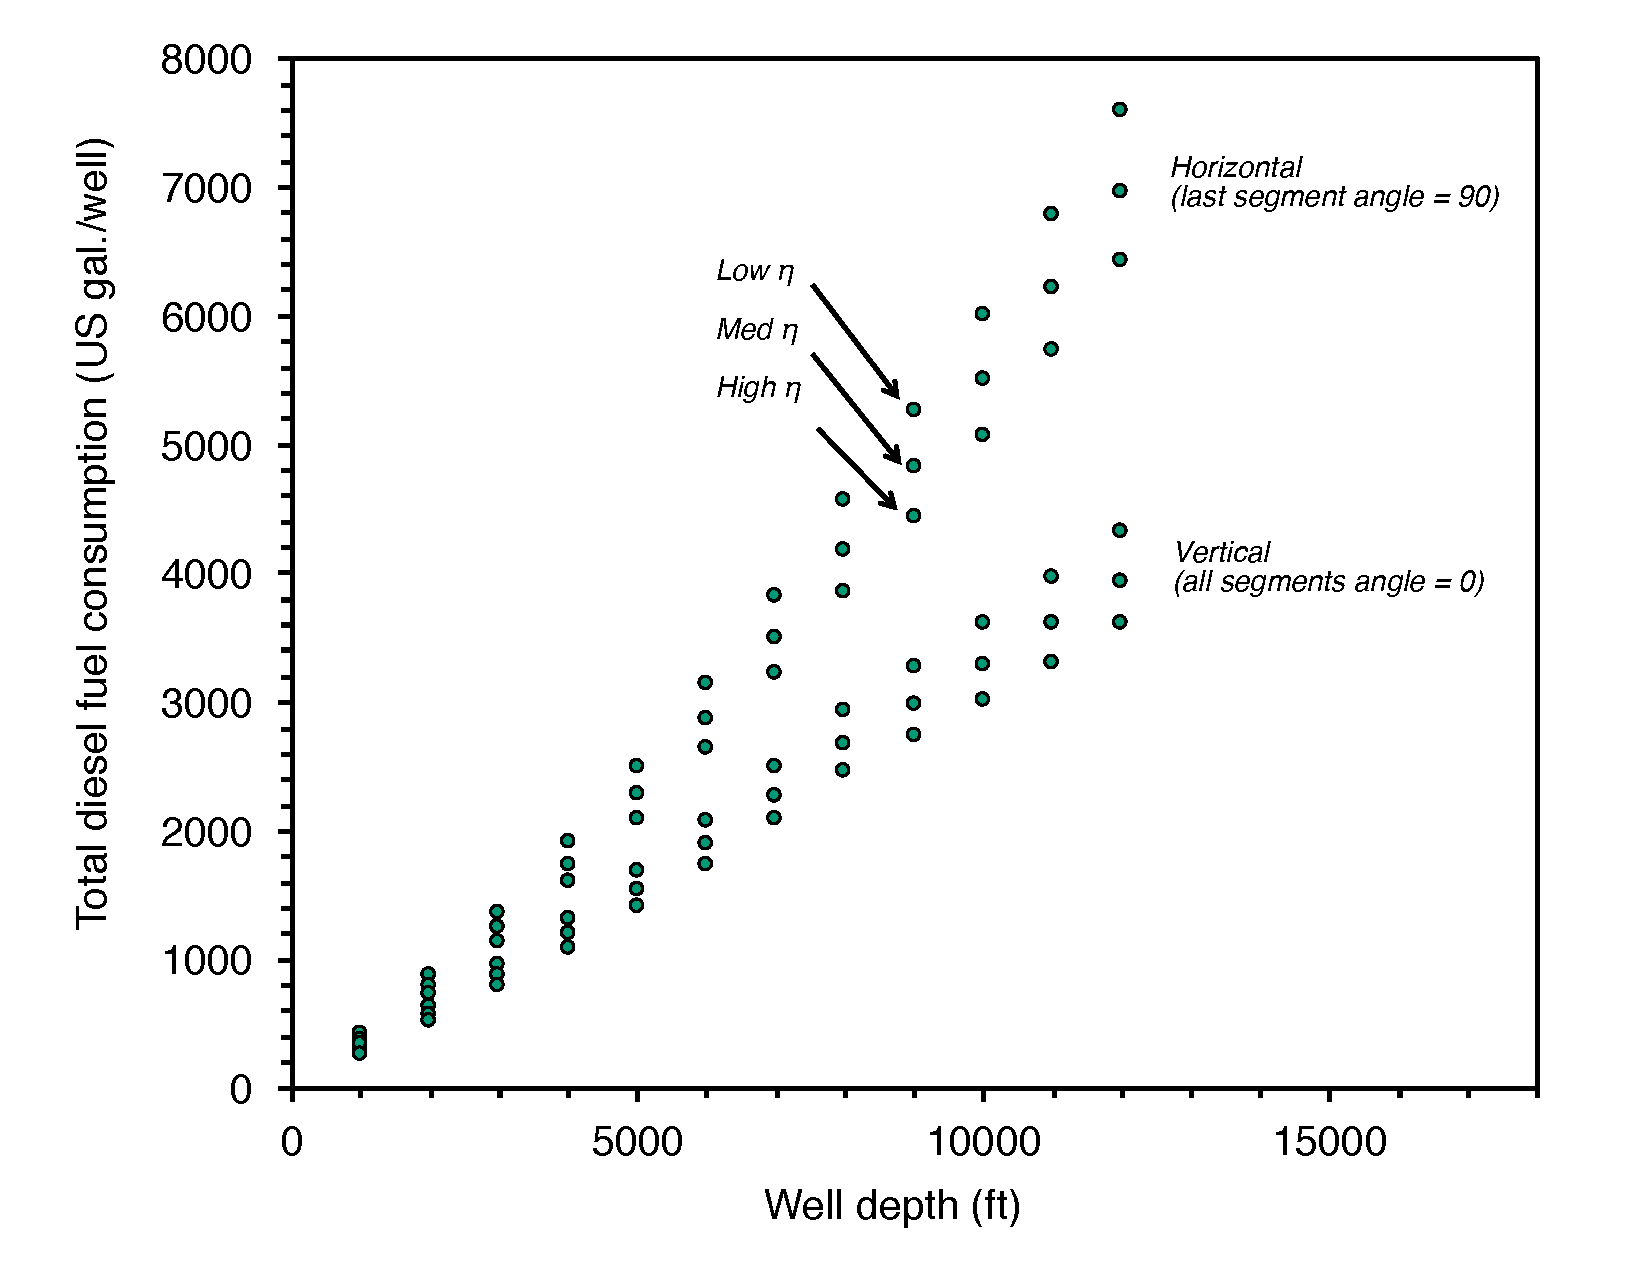
\includegraphics[width=0.8\columnwidth]{images/Drilling3.pdf}
\caption{GHGfrack results for drilling fuel consumption. Only simple wells are represented, and the results are segmented by efficiency and wellbore orientation. Fuel consumption reported in US gallons of diesel (includes both rotary table + mud circulation).}
\label{fig:drilling3}
\end{figure}

Using these segmented results, we construct a drilling intensity factor per-foot of drilled well for vertical wells.  Because the results in Figure \ref{fig:drilling3} are largely linear within a given efficiency setting and well geometry, we can use a linear model segmented by well category. Fuel intensity factors $FI$ [gal diesel fuel/ft.] are constructed separate for each ``line'' in Figure \ref{fig:drilling3} as follows: vertical wells are segmented by well-complexity, well diameter, and assumed efficiency setting.  A linear slope is computed to estimate the fuel intensity factor $FI$ by summing the total fuel use across all wells in a given well complexity-well size category and summing the total distance drilled across all wells in that category:
\begin{equation}
FI_{D}^{v,cat} = \frac{\sum_{i \in cat} F_{D}^{i}}{\sum_{i \in cat} D_{v}^{i}}
\end{equation}
where $i$ is the index for wells, $i \in cat$ represents the subset of all wells $i$ that are included in a given well-complexity, well diameter, and efficiency setting category.  $D_{v}^{i}$ is the vertical distance drilled (TVD) for each vertical well in the particular category.  These tabulated fuel intensity factors $FI$ are included in OPGEE and selected using logic for each field depending on field well construction practices.

To compute the excess fuel required to drill horizontal wells, we compare each horizontal well to the vertical well of the same total drilling distance and compute the additional fuel use associated with making each well have a horizontal segment.  This additional fuel use can then be divided for each well by the length of the horizontal segment. This gives a horizontal well fuel intensity factor $FI$:
\begin{equation}
FI_{D}^{h,cat} = \frac{\sum_{i \in cat} \left(F_{D}^{i,h} - F_{D}^{i,v} \right)}{\sum_{i \in cat} D_{h}^{i}}
\end{equation}
Where $F_{D}^{i,h}$ is the fuel consumed in the horizontal version of well $i$ and $F_{D}^{i,v}$ is the fuel consumed in the vertical version of the same well $i$ [gal diesel].  The horizontal distance $D_{h}$ for a given well is the distance of the terminal well segment (horizontal).  This computation results in an incremental fuel consumption per ft. of horizontal well drilled [gal/ft. horizontal]. 

Using these two factors, we can compute the total fuel required to drill a horizontal or vertical well $i$ using a single expression:
\begin{equation}
F_{D}^{i} =  D_{v}^{i}\left( FI_{D}^{v,i} \right)+ f_h D_{h}^{i} \left(FI_{D}^{v,i} + FI_{D}^{h,i}  \right)
\end{equation}
where $f_h$ is the fraction of wells [0-1] with horizontal segment of length $D_h$ [ft].

Drilling energy consumption must be amortized over the producing life of a well. Also, drilling and development energy must account for drilling of water injection wells. The lifetime productivity of wells varies by orders of magnitude, depending on the quality of the oil reservoir and its size. We include three cases for the productivity of wells from prior studies of embodied energy in oilfield operations \cite{Brandt2015}.  Three options are allowed, corresponding to ``low'', ``medium'', and ``high'' per-well cumulative productivity. These settings correspond approximately to average production in the US, global average, and OPEC average productivity. Numerical values are 150 kbbl/well, 800 kbbl/well and 7,000 kbbl/well, respectively \cite[Supporting Information Table S1]{Brandt2015}.

The energy intensity of drilling per unit of energy produced is therefore calculated as follows: \marginnote{Drilling \& Development 2.3}
%%%%%%%%%%
\begin{equation}
ei_{D} = \frac{F_{D} N_{W}LHV_{di}}{Q_{o,tot} LHV_o} \quad\quad \footnotesize{\text{[mmBtu/mmBtu]}}
\end{equation}
%%%%%%%%%%
where $ei_{DR}$ = energy intensity of drilling [mmBtu/1000 ft]; $h_W$ = average well depth [1000 ft]; $Q_{o,tot}$ = total lifetime productivity per well drilled [bbl oil/well]; and $LHV_o$ = lower heating value of the crude produced [mmBtu LHV/bbl].

The energy intensity of drilling tends to be small when amortized over total well productivity, with values on order 10$^{-6}$ to 10$^{-2}$ mmBtu/mmBtu.

\subsubsection{Emissions from hydraulic fracturing}

The practice of hydraulic fracturing can consume large amounts of energy. This is because modern high-volume multi-stage hydraulic fracturing requires injecting large amounts of fluid at high pressures.  \emph{GHGfrack} models the injection of hydraulic fracturing fluids by accounting for the pressure required for fracturing:
\begin{equation}
\Delta P_{hf} = \Delta P_{fracture} + \Delta P_{fric} - \Delta P_{hydrostatic},
\end{equation}
where $\Delta P_{fracture}$ is the fracturing pressure required to overcome the fracturing gradient [psi], $ \Delta P_{fric}$ is the frictional pressure drop during injection [psi], and $\Delta P_{hydrostatic}$ is the contribution from the hydrostatic head of water in the wellbore [psi].

As in the case of mud pump injection energy, the energy requirements of hydraulic fracturing are calculated from the pressure drop as follows:
\begin{equation}
E_{D}^{hf} = \frac{\Delta P_{hf} Q_{hf}}{1714 \eta} \times t,
\end{equation}
and the fuel consumption due to hydraulic fracturing is computed similarly to the fuel consumption due to drilling:
\begin{equation}
F_{D}^{hf} = \frac{E_{D}^{hf} \eta_{gs}}{LHV_{di}}.
\end{equation}
We compute the fuel consumption due to hydraulic fracturing using \emph{GHGfrack} for numerous cases and use the results to create simple correlations for use in OPGEE.  We use a number of default \emph{GHGfrack} assumptions during the runs, including:
\begin{itemize}
\item Injection string ID = 5 in.
\item Horizontal lateral length = 5000 ft.
\item Fracturing fluid density = 9.0 lbm/gal.
\item Viscosity = 1 cp
\item Pipe roughness = 0.00008 in
\item Length of fracturing stage = 300 ft
\item Number of computational segments = 10
\item Pump efficiency = 65\%
\item Injection time = 48 hr
\end{itemize}
In order to generate the relationships used in OPGEE, we vary two key inputs to the \emph{GHGfrack} hydraulic fracturing module: (1) amount of fracturing fluid injected, and (2) fracturing gradient.  In these runs, the fracturing gradient is varied from 0.6 psi/ft to 1.0 psi/ft in increments of 0.05 psi/ft.  Also, in these runs the amount of fluid injected is varied from 1 to 5 $\times 10^6$ gallons in increments of 1$\times 10^6$ gallons.  Therefore, a total of 45 \emph{GHGfrack} fracturing simulations are performed.

The results from these \emph{GHGfrack} simulations are shown in Figure \ref{fig:fracturing1}.  We fit quadratic functions to each set of results from the same fracturing gradient value.  In each case, the r$^2$ value is $\geq$0.999.  The resulting quadratic function coefficients are used in OPGEE to predict hydraulic fracturing energy use in a particular field based on the volume of fracturing fluid injected.  The equation used is:
\begin{equation}
F_{D}^{hf}=  a V_{hf}^2 + b V_{hf} + c \text{ [gal diesel]}
\end{equation}
where $a$, $b$ and $c$ are fitting constants unique to each fracturing gradient.  The results for the fitting constants $a$, $b$ and $c$ are shown in Table \ref{tab:fracturing_fit}.

\begin{table}
\begin{scriptsize}
\tablefirsthead{\toprule Fracturing gradient [psi/ft]  & $a$ & $b$ & $c$        \\
\midrule}
\tablehead{}
\tabletail{}
\tablelasttail{\bottomrule}
\tablecaption{Constants for quadratic fit of fracturing fuel consumption equation}
\label{tab:fracturing_fit}
\begin{threeparttable}
\begin{supertabular*}{0.6\columnwidth}{p{0.12\columnwidth}p{0.12\columnwidth}p{0.12\columnwidth}p{0.12\columnwidth}}
0.60 & 588.55 & -488.77 & 1184.50 \\
0.65 & 599.49 & -246.27 & 1349.20 \\
0.70 & 511.30 & 575.63  & 964.32  \\
0.75 & 499.47 & 924.06  & 1012.50 \\
0.80 & 566.77 & 1090.40 & 1101.60 \\
0.85 & 570.18 & 1378.20 & 1162.60 \\
0.90 & 523.67 & 1882.70 & 1233.90 \\
0.95 & 664.49 & 1512.60 & 1922.70 \\
1.00 & 477.57 & 3025.40 & 752.02 \\
\end{supertabular*}
\end{threeparttable}
\end{scriptsize}
\end{table}

\begin{figure}[tb]
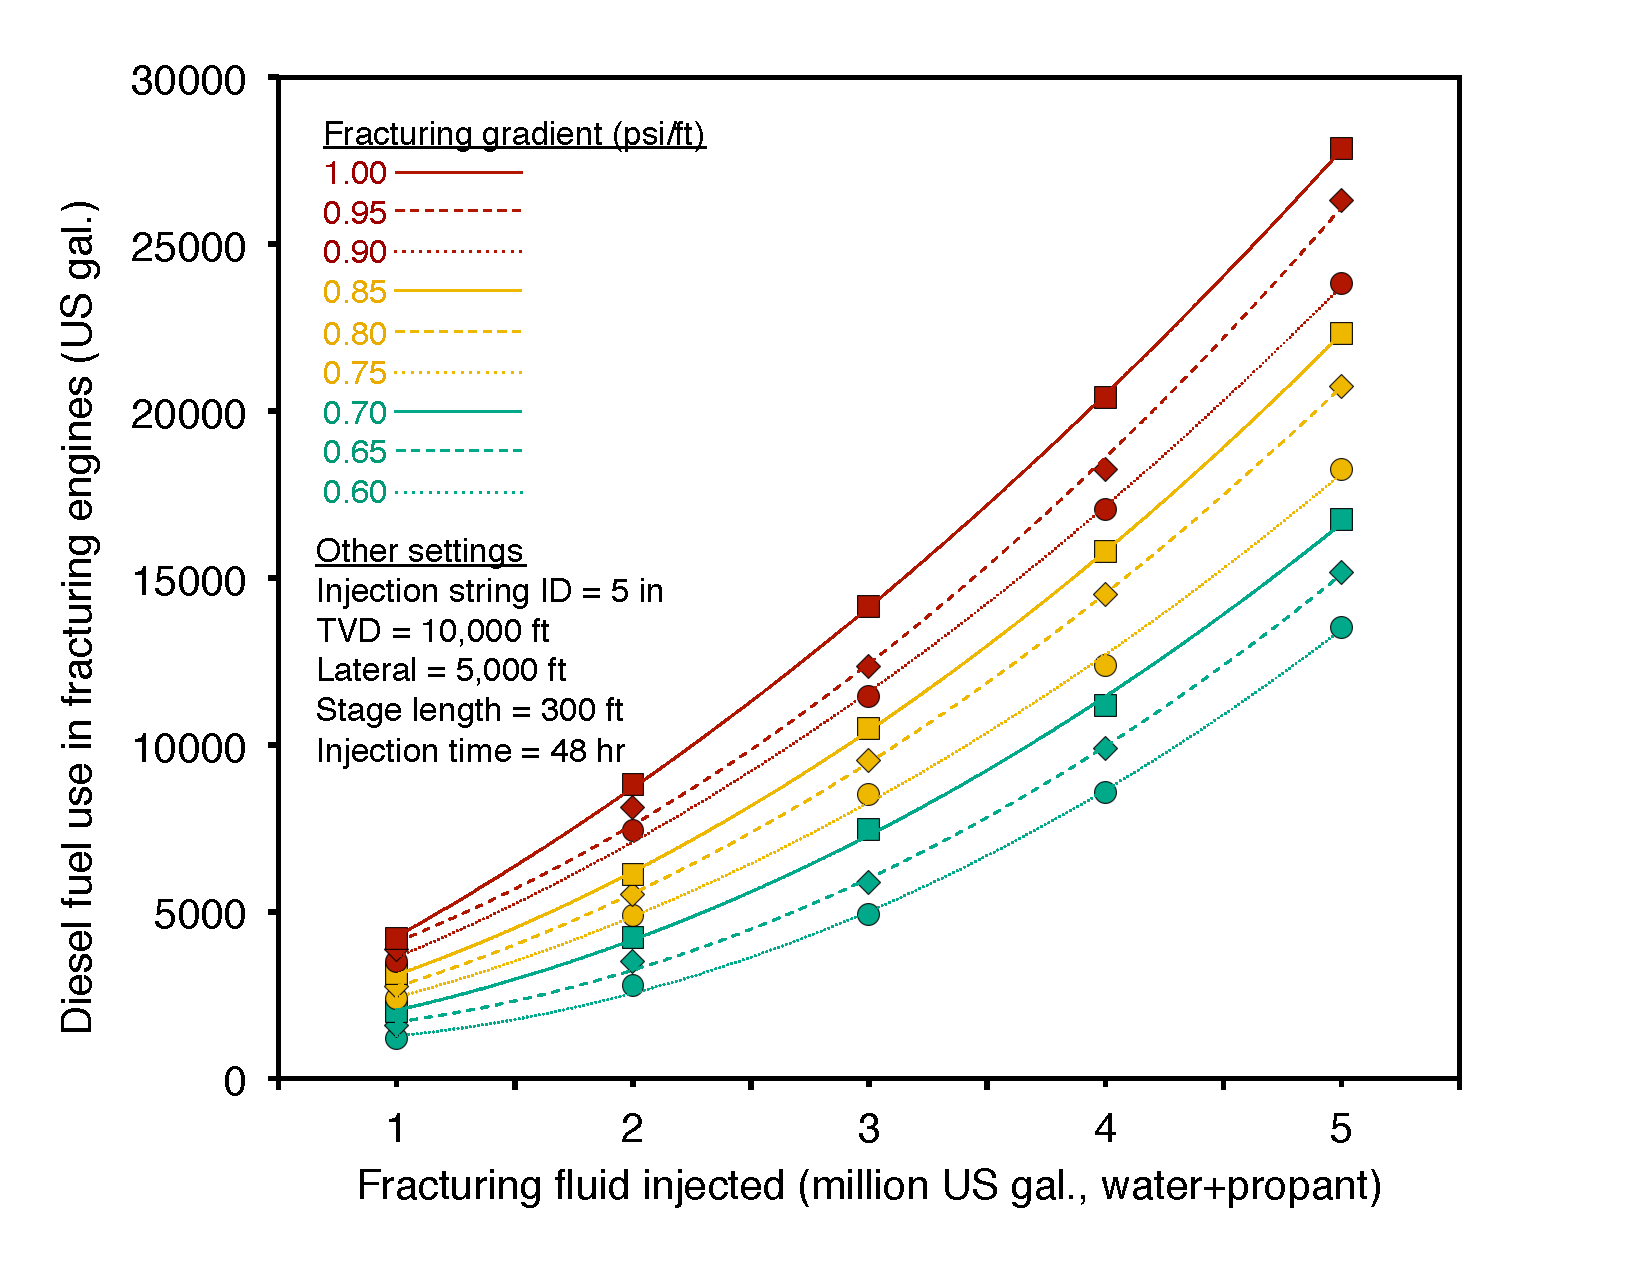
\includegraphics[width=0.8\columnwidth]{images/Fracturing1.pdf}
\caption{Fuel use in hydraulic fracturing as a function of fracturing volume. Each curve represents a different fracturing gradient value, ranging from 0.6 psi/ft to 1.0 psi/ft.}
\label{fig:fracturing1}
\end{figure}

\clearpage

\subsubsection{Emissions from land use impacts}

Land use \marginnote{Drilling \& Development 1.3,2.3} impacts during drilling and field development are included in OPGEE for three categories: soil carbon that is oxidized upon disturbance of land, biomass carbon that is oxidized due to biomass disturbance, and emissions from foregone sequestration, due to the fact that biomass carbon sequestration is slowed on cleared land. For each of these impacts, emissions estimates from Yeh et al. \cite{Yeh2010} are included. Yeh et al. measured impacts over a 150 year \marginnote{Emissions Factors Tables 1.6,1.7} period, which is not in alignment with other analyses that use 30 year land use impact calculations. For this reason, calculations from Yeh et al. were modified to reduce the timeframe for analysis to 30 years, reducing the amount of regrowth possible \cite{Yeh2012}. 

The user has the option to choose a 30 year \marginnote{Drilling \& Development 1.2.13} or 150 year analysis timeframe. The default analysis timeframe is set to 30 years.

In order to estimate land use GHG emissions, three settings are required. \marginnote{Drilling \& Development 1.1.3,1.1.4} First, the crude production method must be chosen. The options for crude production method include conventional production via wellbore (primary, secondary, and tertiary recovery of conventional and heavy hydrocarbons, including in situ recovery of bitumen) and mining-based production of bitumen. 

Next, the carbon richness of the ecosystem is specified. \marginnote{Drilling \& Development 1.1.10} Options include low, moderate, and high carbon richness. Low carbon richness estimates are derived from California production in the semi-arid to arid central valley of California \cite{Yeh2010}. The high carbon richness estimates are derived from forested regions in Alberta (e.g., rocky mountain foothills) \cite{Yeh2010}. Moderate carbon richness is considered a mixed ecosystem with carbon richness between these ecosystems.

Lastly, the intensity of field development must be specified. \marginnote{Drilling \& Development 1.1.11} High intensity field development corresponds to high fractional disturbance, such as in a field drilled on tight spacing. Low intensity field development corresponds to a sparsely developed field with little fractional disturbance. Moderate field development occurs between these two extremes. Work by Yeh et al. \cite{Yeh2010} can be consulted for satellite images of low and high field development intensity.

Emissions associated with each choice \marginnote{Emissions Factors Tables 1.6,1.7} are shown in Table \ref{tab:default_land_use_emissions} in units of gCO$_2$eq GHGs per MJ of crude oil produced.

\subsection{Defaults for drilling \& development}

Default values for drilling \& development calculations are shown in Tables \ref{tab:defaults_drilling} and \ref{tab:default_land_use_emissions}. 

\begin{table}
\begin{scriptsize}
\caption{Land use GHG emissions for 30 year analysis period from field drilling and development in OPGEE for conventional oil operations [g CO$_2$ eq./MJ of crude oil produced]. Data from Yeh et al \cite{Yeh2010}.}
\label{tab:default_land_use_emissions}
\begin{tabular}{p{0.13\columnwidth}p{0.06\columnwidth}p{0.06\columnwidth}p{0.06\columnwidth}p{0.06\columnwidth}p{0.06\columnwidth}p{0.06\columnwidth}p{0.06\columnwidth}p{0.06\columnwidth}p{0.06\columnwidth}}
\toprule
& \multicolumn{3}{p{0.25\columnwidth}}{Low carbon stock } & \multicolumn{3}{p{0.25\columnwidth}}{Moderate carbon stock } & \multicolumn{3}{p{0.25\columnwidth}}{High carbon stock}\\
& \multicolumn{3}{p{0.25\columnwidth}}{(semi-arid grasslands)} & \multicolumn{3}{p{0.25\columnwidth}}{(mixed)} & \multicolumn{3}{p{0.25\columnwidth}}{(forested)}\\
\cmidrule{2-4} \cmidrule{5-7} \cmidrule{8-10}
& Low int. & Med. int. & High int. & Low int. & Med. int. & High int. & Low int. & Med. int. & High int.\\
\midrule
Soil carbon & 0.03 & 0.13 & 0.35 & 0.22 & 0.57 & 1.93 & 0.40 & 1.01 & 3.51\\
Biomass & 0.00 & 0.00 & 0.00 & 0.34 & 0.68 & 1.47 & 0.68 & 1.36 & 2.94\\
Foregone seq.\ & 0.00 & 0.00 & 0.00 & 0.01 & 0.01 & 0.01 & 0.01 & 0.01 & 0.02\\
\bottomrule
\end{tabular}
\end{scriptsize}
\end{table}



\begin{table}
\begin{scriptsize}
\caption{Land use GHG emissions for 150 year analysis period from field drilling and development in OPGEE for conventional oil operations [g CO$_2$ eq./MJ of crude oil produced]. Data from Yeh et al \cite{Yeh2010}.}
\label{tab:default_land_use_emissions}
\begin{tabular}{p{0.13\columnwidth}p{0.06\columnwidth}p{0.06\columnwidth}p{0.06\columnwidth}p{0.06\columnwidth}p{0.06\columnwidth}p{0.06\columnwidth}p{0.06\columnwidth}p{0.06\columnwidth}p{0.06\columnwidth}}
\toprule
& \multicolumn{3}{p{0.25\columnwidth}}{Low carbon stock } & \multicolumn{3}{p{0.25\columnwidth}}{Moderate carbon stock } & \multicolumn{3}{p{0.25\columnwidth}}{High carbon stock}\\
& \multicolumn{3}{p{0.25\columnwidth}}{(semi-arid grasslands)} & \multicolumn{3}{p{0.25\columnwidth}}{(mixed)} & \multicolumn{3}{p{0.25\columnwidth}}{(forested)}\\
\cmidrule{2-4} \cmidrule{5-7} \cmidrule{8-10}
& Low int. & Med. int. & High int. & Low int. & Med. int. & High int. & Low int. & Med. int. & High int.\\
\midrule
Soil carbon & 0.03 & 0.13 & 0.35 & 0.10 & 0.35 & 1.50 & 0.16 & 0.57 & 2.65\\
Biomass & 0.00 & 0.00 & 0.00 & 0.01 & 0.09 & 0.33 & 0.02 & 0.17 & 0.65\\
Foregone seq.\ & 0.00 & 0.00 & 0.00 & 0.02 & 0.03 & 0.05 & 0.03 & 0.05 & 0.09\\
\bottomrule
\end{tabular}
\end{scriptsize}
\end{table}

\begin{landscape}
\begin{scriptsize}
\tablefirsthead{\toprule Param. & Description & Eq. no. & Default & Literature range & Unit & Sources & Notes\\
\midrule}
\tablehead{ \multicolumn{5}{p{1\columnwidth}}{\textit{Continued from previous page}}\\ \toprule Param. &Description & Eq. no. &Default & Literature range & Unit & Sources & Notes \\ 
\midrule }
\tabletail{\bottomrule \multicolumn{5}{p{1\columnwidth}}{\textit{Continued on next page...}}\\}
\tablelasttail{\bottomrule}
\tablecaption{Default inputs for drilling calculations.}
\label{tab:defaults_drilling}
\begin{threeparttable}
\begin{supertabular*}{1\columnwidth}{p{0.05\columnwidth}p{0.3\columnwidth}p{0.05\columnwidth}p{0.05\columnwidth}p{0.15\columnwidth}p{0.15\columnwidth}p{0.05\columnwidth}p{0.05\columnwidth}}
$D_{v}$ 		& Vertical depth of wells						&  & 7240 		& 100-20,000 	&[ft] &  & a\\ 
$D_{h}$ 		& Length of horizontal segment of well			& - & 5000 	& 1000-10,000 	&[ft] &  & a\\ 
$f_h$		& Fraction of wells with horizontal segment		& - & 0		& 0 - 1		& [fraction horizontal] & & \\
$FI_{D}^{h} $ 	& Horizontal drilling incremental fuel intensity		& - &0.380 	& 0.218 - 0.459 & [gal/ft. horizontal] & \cite{Vafi2016b} & b \\
$FI_{D}^{v} $ 	& Vertical drilling fuel intensity			 		& - &0.404 	& 0.226 - 0.724 & [gal/ft.] & \cite{Vafi2016b} & b \\
$N_W$ 		& Number of total wells, prod. and inj.			& - & 13 		& - & [Wells] 	& - & c \\
$Q_{o,tot}$ 	& Cumulative production per well over life of well 	& - & 800 		& 150 - 7,000 & [kbbl/well] &\cite{Brandt2015} & d\\
$LHV_{di}$ 	& Lower heating value of diesel fuel				& - & 128.5 	& 128.5 		& [mBtu/gal] & \cite{Wang2009} & e \\
$LHV_{o}$ 	& Lower heating value of crude oil 				& - & 5.51 	& 5.15 - 6.18 	& [mmBtu/bbl] & \cite{Schmidt1985} & e \\
\end{supertabular*}
\begin{tablenotes}
\item[a] Low and high drilling efficiency constants found from fitting data. Default set to low intensity.
\item[b] Exponential increase with drilling depth. Low intensity drilling actually has slightly higher growth rate.
\item[c] Default well depth chosen to be depth of field $h$. Range of field depths is large in practice.
\item[d]Cumulative production per well from Brandt \cite{Brandt2015}. 
\item[e] Lower heating value of crude depends on density and composition, we use relationship from Schmidt \cite{Schmidt1985}.
\end{tablenotes}
\end{threeparttable}
\end{scriptsize}

\end{landscape}



\clearpage



%%%%%%%%%%%%%%%%%%%%%%%%%%%%%%%%%%%%%%%%%%%%%%%%%%%%%%%%%%%%%%
\section {Reservoir}\label{sec:reservoir}


Pressure in the reservoir drives fluids toward the (lower pressure) wellbore bottom. The amount of flow depends on the pressure differential and the properties of the rock.  At the wellbore bottom the fluids have some bottomhole flowing pressure that serves as the baseline pressure in artificial lifting calculations (see below). In addition to artificial lifting, water can be injected into the reservoir to support reservoir pressure and increase oil recovery \cite[p. 1]{Rose1989}. 

The streams flowing into and out of the reservoir-well interface process are shown in Figure \ref{fig:reservoir_PF} and are listed in Table \ref{tab:reservoir_PF}.  
The secondary inputs to the reservoir sheet are listed in Table \ref{tab:reservoir_SI}.

\clearpage

%%%%%%%%%%%
\begin{table}
\caption{Streams flowing into and out of the reservoir-well interface process. I/O denotes input or output stream}
\label{tab:reservoir_PF}
\begin{scriptsize}
\begin{tabularx}{1\columnwidth}{p{0.32\columnwidth}p{0.05\columnwidth}p{0.04\columnwidth}p{0.32\columnwidth}p{0.05\columnwidth}p{0.05\columnwidth}}
\toprule
Flow name							& Stream   			& I/O 	& Source/Destination       			& Units 			&  Notes\\ 
\midrule
Oil from reservoir						& \stream{1}			& I		& Reservoir					& [t/d]			& 			\\
Water from reservoir						& \stream{100}			& I		& Reservoir					& [t/d]			& 			\\
Gas from reservoir						& \stream{25}			& I		& Reservoir					& [t/d]			&			\\
\midrule
Oil at well bottom						& \stream{3}			& O		& Well/downhole pump			& [t/d]			&			\\
Water at well bottom						& \stream{101}			& O		& Well/downhole pump			& [t/d]			&			\\
Gas at well bottom						& \stream{26}			& O		& Well/downhole pump			& [t/d]			&			\\
\bottomrule
\end{tabularx}
\end{scriptsize}
\end{table}
%%%%%%%%%%%



%%%%%%%%%%%
\begin{figure}
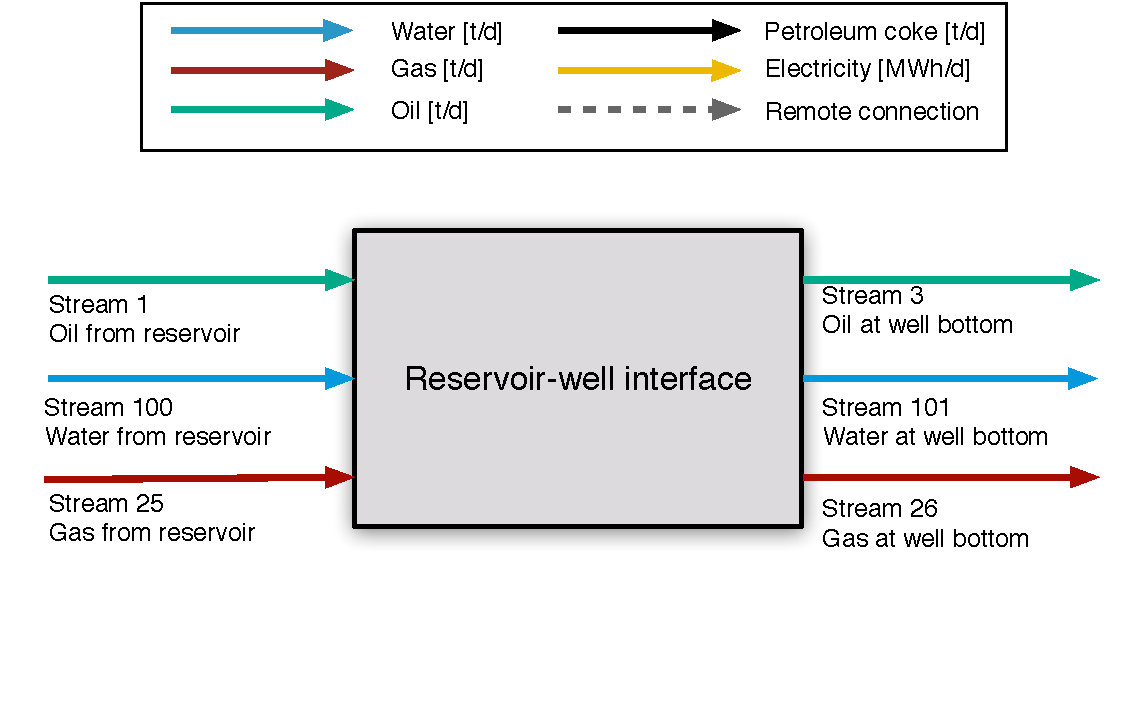
\includegraphics[width=0.85\columnwidth]{images/Reservoir_PF.pdf}
\caption{Streams flowing into and out of reservoir-well interface. All streams measured in tonnes per day excepting electricity which is measured in MWh/d.}
\label{fig:reservoir_PF}
\end{figure}
%%%%%%%%%%%





\clearpage

An important part of the reservoir flow problem is to understand the nature of flow and in what phases the hydrocarbon material will be flowing to the wellbore.

The bubblepoint pressure is the pressure at which the solution gas will start to evolve from the oil into a separate gas phase (i.e., the gas will start to bubble out of the oil).  We use the  \marginnote{Reservoir \\ M68} bubblepoint pressure relationship of Al-Shammasi (1999), as reproduced in \cite[vol 1, Table 6.6]{Fanchi2007}:
\begin{equation}
P_{b} =\gamma_{o}^{a_1}\times\left[R_b \gamma_g (T_r+459.67)\right]^{a_2}\times e^{(-a_3 \gamma_o \gamma_g)} \eqnunit{psi}
\label{eq:BPP}
\end{equation}

where $P_b$ is the bubblepoint pressure of the oil, $\gamma_o$ is the oil specific gravity (water = 1), $\gamma_g$ is the gas specific gravity (air = 1), $T_r$ is the reservoir temperature [$^\circ$F], and $a_1$, $a_2$, and $a_3$ are fitting constants.  $R_b$ is the bubblepoint solution gas oil ratio [scf/bb], discussed below. At a given pressure, this equation can be re-arranged to find the amount of gas in solution, so it is used to compute the solution GOR for various conditions as well \cite[p. 273]{Fanchi2007}

The average reservoir  \marginnote{Active Field \\ K69} temperature $T_r$ is either given as a data input or filled with an OPGEE smart default given the reservoir depth. The default relationship is: 
\begin{equation}
T_r = 70 + 1.8 \frac{h}{100}  \eqnunit{$^\circ$F}
\label{eq:Tr}
\end{equation}
where 70 $^\circ$F is the default yearly average surface temperature, $h$ is the reservoir depth [ft], and 1.8 is the geothermal gradient in $^\circ$F per 100 ft.

The amount of gas in solution at the bubblepoint is important for modeling flow. Valko and McCain (2003) give a means to estimate the bubble point gas-oil ratio from the separator gas oil ratio \cite{Valko2003}. Since OPGEE takes separator gas oil ratio $GOR$ as an input, we use this correlation \cite[eq. 3-3]{Valko2003}: \marginnote{Reservoir \\ M67}
\begin{equation}
R_b = 1.1618 \times GOR \eqnunitfrac{scf}{bbl} 
\label{eq:GORb}
\end{equation}
where $GOR$ is the separator GOR, which is most commonly reported in the literature, and as drawn from the \sheet{Active Field} working sheet.

The equation given above for bubblepoint pressure \ref{eq:BPP} can be rearranged to solve for the solution gas oil ratio. Given an actual reservoir pressure below the bubblepoint, the amount of gas in solution at reservoir conditions can be solved for \cite[Vol. 1, sec 6.5]{Fanchi2007}. \marginnote{Reservoir \\ M70}



The water formation volume factor, $B_w$, or the ratio of bbl of water in the reservoir to bbl of water at stock tank conditions [bbl/STB] is given by a correlation from McCain, reproduced in Fanchi 2007 \cite[p. 483]{Fanchi2007}:\marginnote{Reservoir \\ M79}
\begin{equation}
B_w = (1+\Delta V_{wp})(1+ \Delta V_{wT})  \eqnunitfrac{bbl}{STB}
\end{equation}
where the first term is the change in volume due to pressure and the second is the change in volume due to temperature. These are computed as follows:
\begin{equation}
\Delta V_{wp} = a_1+ a_2 T_r + a_3 T_r^2
\end{equation}
\begin{equation}
\Delta V_{wT} = a_4 p_r T_r+ a_5 p_r^2 T_r + a_6 p_r + a_7 p_r^2
\end{equation}
These correlations must be applied to the \marginnote{Reservoir \\ M78}density of water at standard conditions, which varies with the salinity of the water.

The productivity index, PI, is defined as \cite[p. 23]{Takacs2005}:
%%%%%%%%%%
\begin{equation} \label{eq:pressure_drawdown}
\text{PI} = \frac{Q_{l,W}}{(p_{r}-p_{wf})} \eqnunitfrac{bbl}{psi-d}
\end{equation}
%%%%%%%%%%
where PI = well productivity index [bbl liquid/psi-d]; $Q_{l,W}$ = liquid production per well [bbl liquid/d]; $p_{r}$ = average reservior pressure [psi]; and $p_{wf}$ = wellbore pressure [psi]. The increase in production requires an increase in pressure drawdown at a constant productivity index. In OPGEE a default productivity index of 3.0 [bbl liquid/psi-d] is assumed to calculate the pressure drawdown. The user has to control the inputs to satisfy the condition of $p_{wf}$ $\geq$ 0.
The pressure for lifting can either be applied by a downhole pump or by gas lift; in OPGEE these methods may be used individually or simultaneously. \newline


[JEFF: ADD DESCRIPTION OF GAS PHASE PRESSURE DROP]




\begin{table}
\caption{Streams flowing into and out of the wellbore/downhole pump process. I/O denotes input or output stream}
\label{tab:wellbore_PF}
\begin{scriptsize}
\begin{tabularx}{1\columnwidth}{p{0.3\columnwidth}p{0.05\columnwidth}p{0.1\columnwidth}p{0.1\columnwidth}p{0.15\columnwidth}p{0.05\columnwidth}p{0.05\columnwidth}}
\toprule
Parameter name					& Eq. term			& Default value   & Range		& Units 	& Source			      			& Notes 		\\ 
\midrule
Excess pressure in injection well		&					& 500		&			& [psi]	& Assumption					& \\
Temperature of fluids at well bottom		&					& 150		&			& [$^\circ$F] & Assumption				& \\
Reservoir permeability				&					& 100		&			& [mD]	& Assumption					& \\
Reservoir pay thickness				&					& 500		&			& [ft]		& Assumption					& \\
Bubblepoint pressure constant 1		&	$a_1$			& 5.527215 	& - 			&  [-] 	& \cite{AlShammasi1999} 			& \\
Bubblepoint pressure constant 2		&	$a_2$			& 0.783716 	& - 			&  [-] 	& \cite{AlShammasi1999} 			& \\
Bubblepoint pressure constant 3		&	$a_3$			& 1.841408 	& - 			&  [-] 	& \cite{AlShammasi1999} 			& \\
Oil FVF constant 1					&	$a_1$			& 1 		  	& - 			&  [-] 	& \cite{AlShammasi1999} 			& \\
Oil FVF constant 2					&	$a_2$			& 5.253E-07 	& - 			&  [-] 	& \cite{AlShammasi1999} 			& \\
Oil FVF constant 3					&	$a_3$			& 0.000181 	& - 			&  [-] 	& \cite{AlShammasi1999} 			& \\
Oil FVF constant 4					&	$a_4$			& 0.000449 	& - 			&  [-] 	& \cite{AlShammasi1999} 			& \\
Oil FVF constant 5					&	$a_5$			& 0.000206 	& - 			&  [-] 	& \cite{AlShammasi1999} 			& \\
Water FVF constant 1				&	$a_1$			& -0.010001 	& - 			&  [-] 	& \cite{AlShammasi1999} 			& \\
Water FVF constant 2				&	$a_2$			& 0.0001334 	& - 			&  [-] 	& \cite{McCain1990} 				& \\
Water FVF constant 3				&	$a_3$			& 5.507e-7	& - 			&  [-] 	& \cite{McCain1990} 				& \\
Water FVF constant 4				&	$a_4$			& -1.95e-9		& - 			&  [-] 	& \cite{McCain1990}				& \\
Water FVF constant 5				&	$a_5$			& -1.73e-13	& - 			&  [-] 	& \cite{McCain1990} 				& \\
Water FVF constant 6				&	$a_6$			& -3.59e-7 	& - 			&  [-] 	& \cite{McCain1990} 				& \\
Water FVF constant 7				&	$a_7$			& -2.25e-10 	& - 			&  [-] 	& \cite{McCain1990} 				& \\
Bubblepoint gas-oil-ratio 				&	$GOR_b$			& 1055 		& -			& [scf/bbl] & \cite{Valko2003} 				& \\
Reservoir temperature				& 	$T_r$			& 200 		& -			& [$^\circ$F] & 							& \\
Specific gravity of gas				&	$\gamma_g$ 	 	& 0.69		& 0.6-0.8 		& [g/g] 	&  & 							a \\
Specific gravity of oil					&	$\gamma_o$ 	 	& 0.88 		& 0.75-1.05	& [g/g] 	& \cite{Scmidth1985} 			& b \\
\midrule
\multicolumn{7}{p{1\columnwidth}}{\emph{a} - Computed from gas properties using MW of gases and gas composition. At OPGEE defaults, gas sg = 0.69.}\\
\multicolumn{7}{p{1\columnwidth}}{\emph{b} - Specific gravity of oil is a function of reported oil API gravity. Lookup from \cite{Schmidt1985} in \sheet{Fuel Specs} sheet.}\\
\bottomrule
\end{tabularx}
\end{scriptsize}
\end{table}









\clearpage

%%%%%%%%%%%%%%%%%%%%%%%%%%%%%%%%%%%%%
\section{Wellbore/Downhole Pump}

As production from a field proceeds the reservoir pressure will decrease. To maintain economic viability, artificial lift equipment is used to enhance production rates. Most commonly, energy is added to the reservoir fluids through the use of a downhole pump \cite[p. 2]{Takacs2005}. Another method is gas lifting, which entails injecting gas into the production string to decrease the density of the column of oil and water in the production tubing. 

The streams flowing into and out of the wellbore/downhole pump process are shown in Figure \ref{fig:wellbore_PF} and are listed in Table \ref{tab:reservoir_PF}.


\clearpage

%%%%%%%%%%%
\begin{table}
\caption{Streams flowing into and out of the wellbore/downhole pump process. I/O denotes input or output stream}
\label{tab:wellbore_PF}
\begin{scriptsize}
\begin{tabularx}{1\columnwidth}{p{0.32\columnwidth}p{0.05\columnwidth}p{0.04\columnwidth}p{0.32\columnwidth}p{0.05\columnwidth}p{0.05\columnwidth}}
\toprule
Flow name							& Stream   			& I/O 	& Source/Destination       			& Units 			&  Notes\\ 
\midrule
Oil at well bottom						& \stream{3}			& I		& Reservoir/well interface			& [t/d]			&			\\
Water at well bottom						& \stream{101}			& I		& Reservoir/well interface			& [t/d]			&			\\
Gas at well bottom						& \stream{26}			& I		& Reservoir/well interface			& [t/d]			&			\\
Fuel gas - Downhole pump				& \stream{150}			& I		& Fuel gas system				& [t/d]			&			\\
Electricity - Downhole pump				& \stream{175}			& I		& Electricity generation and imports	& [MWh/d]			& 			\\
Lifting gas to wellbore					&\stream{42}			& I		& Lifting gas compressor			& [t/d]			&			\\
\midrule
Oil at wellhead							& \stream{4}			& O		& Separation					& [t/d]			&			\\
Water at wellhead						& \stream{102}			& O		& Separation					& [t/d]			&			\\
Gas at wellhead						& \stream{27}			& O		& Separation					& [t/d]			&			\\
Wellhead leaks to air						& \stream{250}			& O		& Environment - Atmosphere		& [t/d]			&			\\	
\bottomrule
\end{tabularx}
\end{scriptsize}
\end{table}
%%%%%%%%%%%


%%%%%%%%%%%
\begin{figure}
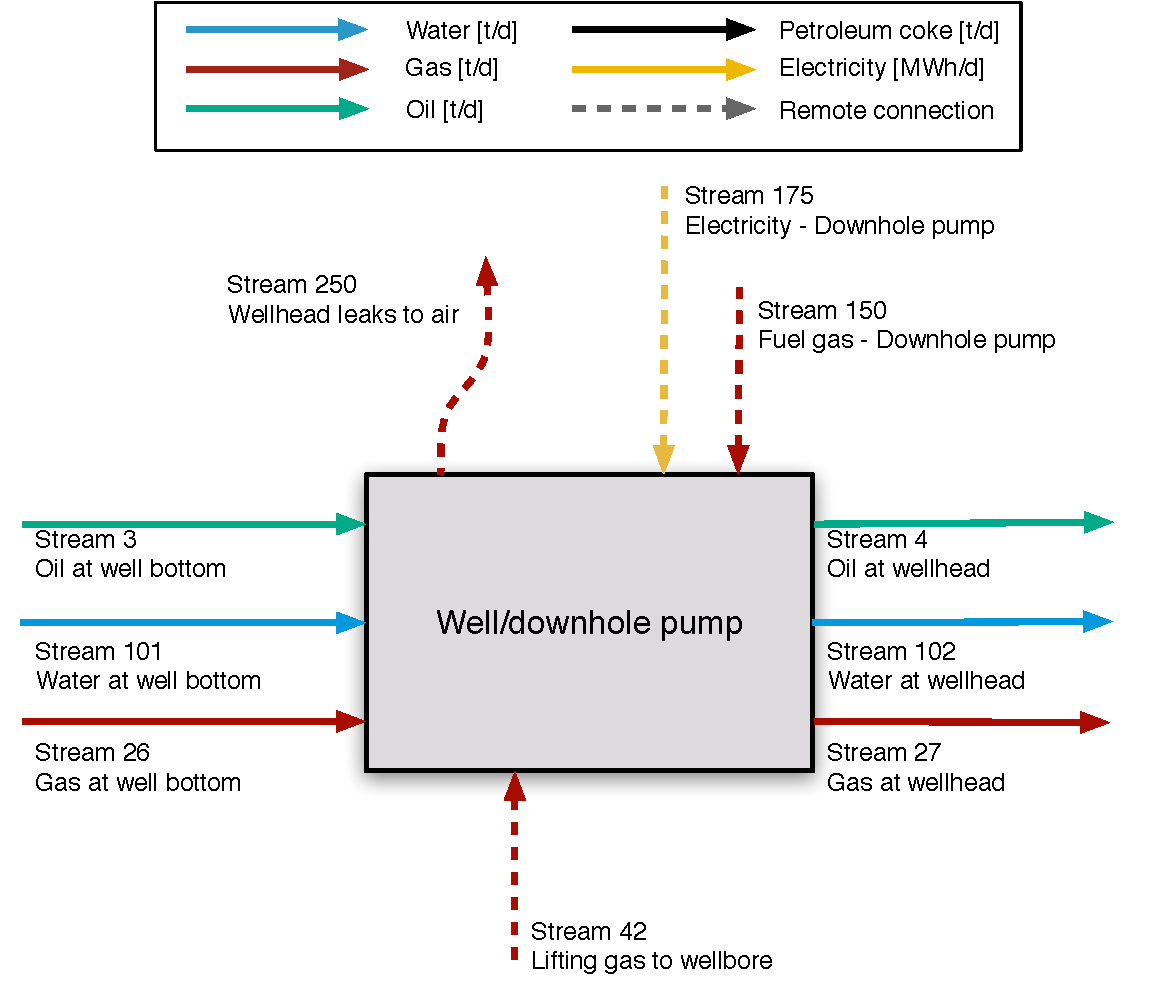
\includegraphics[width=0.85\columnwidth]{images/Wellbore_downhole_pump_PF.pdf}
\caption{Streams flowing into and out of the wellbore/downhole pump process. All streams measured in tonnes per day excepting electricity which is measured in MWh/d.}
\label{fig:wellbore_PF}
\end{figure}
%%%%%%%%%%%


%%%%%%%%%%%
\begin{table}
\caption{Secondary parameter inputs to the wellbore/downhole pump worksheet}
\label{tab:wellbore_SI}
\begin{scriptsize}
\begin{tabularx}{1\columnwidth}{p{0.5\columnwidth}p{0.05\columnwidth}p{0.1\columnwidth}p{0.1\columnwidth}p{0.05\columnwidth}}
\toprule
Parameter name						& Default value   		& Units 	& Source			      			& Notes 		\\ 
\midrule
Concentration of dissolved solids 			& 5000				& [mg/l]	& \cite{Vlasopoulous2006}			& -			\\
Wellhead pressure						& 1000				& [psi] 	& \cite{Manning1991}			& -			\\
Wellhead temperature					& 150				& [$^\circ$F]	& Assumption				& -			\\
Friction factor							& 0.02				& [-]		& \cite{Lake?}					& -			\\
\bottomrule
\end{tabularx}
\end{scriptsize}
\end{table}
%%%%%%%%%%%

\clearpage


Most common artificial lifting and improved oil recovery techniques are included in OPGEE. These include: downhole pump, gas lift, water flooding, gas flooding, and steam injection. In the \sheet{Inputs} worksheet the user is prompted to choose a combination of techniques applicable to the modeled operation. 

A complete list of emissions sources from production, along with their estimated magnitude, is shown in Table \ref{tab:production_sources}. A list of all of the equation parameters, including their default values and sources, is included in Table \ref{tab:defaults_production}.

Energy for lifting is required to overcome the pressure traverse, i.e., the pressure drop between the subsurface reservoir and the surface wellhead. The pressure traverse arises due to two factors: (i) flow against gravity, and (ii) frictional losses. The pressure required for lifting is calculated by adding the wellhead pressure to the pressure traverse and subtracting the wellbore pressure. The artificial lifting methods that can be chosen in OPGEE are: (i) downhole pump, and (ii) gas lift. The pressure required for lifting is equal to the discharge pressure of the downhole pump. The power required to generate the required discharge pressure depends on the discharge flow rate and pump efficiency. Finally the energy required to drive the pump is calculated based on the power requirement (expressed as brake horsepower). 

The calculation of the energy required in water injection- and gas injection- based EOR uses the user inputs for injection volume and discharge pressure. Smart defaults are in place to help assign the discharge pressure taking into account the well depth and frictional losses. 

The energy required for steam flooding requires rigorous modeling of steam generation. An additional complexity is caused by the modeling of electricity co-generation at steam projects. These calculations are explained in Section\,\ref{sec:steam_injection}, which covers steam generation emissions.

In the case of gas lift, if the user enters the volume of gas injected and the discharge pressure, OPGEE will compute the compression energy. However, OPGEE is not sensitive to changes in the gas lift, i.e. the dynamics between the volume of gas lift and the lifting head are not considered. The calculation of these dynamics is beyond the scope of a linear GHG estimator. This requires a two phase flow model, which is not included in OPGEE \version.

% list of the parameters used is shown in Table\,\ref{tab:production_calculations_parameters}. 

Default values for production and extraction calculations are shown in Table \ref{tab:defaults_production}. 


\subsubsection{Oil specific gravity}

The specific gravity of crude oil is usually reported as API gravity, measured at $60\,^{\circ}\mathrm{F}$. The API gravity is related to the specific gravity $\gamma_o$ by: \marginnote{Production \& Extraction 2.1.1} 
%%%%%%%%%%
\begin{equation}\label{eq:production_API_gravity}
^{\circ}\text{API}=\frac{141.5}{\gamma _{o}}-131.5 \begin{footnotesize}\quad\quad\text{[-]}\end{footnotesize} 
\end{equation}
%%%%%%%%%%
where API gravity and $\gamma_o$ are dimensionless measures. The specific gravity is the ratio of the oil density to the density of water \cite[p. 478]{Mcallister2009}.

\subsubsection{Gas specific gravity}

The specific gravity of associated gas is calculated as \cite[p. 10]{Takacs2005}: \marginnote{Production \& Extraction 2.1.4} 
%%%%%%%%%%
\begin{equation} \label{eq:gas_gravity}
\gamma _{g}=\frac{\rho _{gsc}}{\rho _{asc}} \begin{footnotesize} \quad\quad\text{[-]} \end{footnotesize}
\end{equation}
%%%%%%%%%%
where $\rho _{gsc}$ = gas density at standard conditions [\unitfrac{lbm}{ft$^3$}]; and $\rho _{asc}$ = air density at standard conditions [\unitfrac{lbm}{ft$^3$}]. Standard temperature is 60 $^{\circ}${F}; standard pressure is 14.7 psia \cite[p. 35]{Manning1991}. The gas density at standard conditions is calculated using:
%%%%%%%%%%
\begin{equation} \label{eq:gas_density}
\rho _{gsc}=\frac{p_{b} \text{MW$_{g}$}}{\text{R} T_{b}} \begin{footnotesize} \quad\quad \left[\frac{\text{lbm}}{\text{ft$^3$}}\right] \end{footnotesize}
\end{equation}
%%%%%%%%%%
where MW$_{g}$ = molecular weight of the associated gas mixture [\unitfrac{lbm}{lbmol}]; $p_{b}$ = base pressure [psia]; and $T_{b}$ = base temperature [$^{\circ}$R]; R = gas constant [\unitfrac{ft$^3$-psia}{lbmol-$^{\circ}$R}]. The molecular weight is calculated from the molecular weights and molar fractions of the gas constituents.




\subsubsection{Well pressure traverse}

The pressure traverse is the total pressure required to lift the crude oil mixture against gravity and overcome friction and kinetic losses. This is equal to the pressure drop along the well tubing from the wellbore to the wellhead. This pressure drop has two main components: (i) the elevation component, which is the pressure drop due to gravity; and (ii) the friction component, which is the pressure drop due to liquid contact with the inner walls of the well tubing.


The first step in the estimation of the pressure traverse is the calculation of the total head as: \marginnote{Production \& Extraction 1.2.2,2.2.1} 
%%%%%%%%%%
\begin{equation} \label{eq:total_head}
h_{tot}= h_{el} + h_{f} \begin{footnotesize} \quad\quad\text{[ft]} \end{footnotesize}
\end{equation}
%%%%%%%%%%
where $h_{tot}$ = total head [\unit{ft}]; $h_{el}$ = well depth [\unit{ft}]; and $h_{f}$ = friction head [\unit{ft}]. The friction head is calculated using the Darcy formula \cite[p. 447]{Mcallister2009}:
%%%%%%%%%%
\begin{equation} \label{eq:friction_head}
h_{f}=\frac{fh_{el}{v_{l,W}^2}}{2D_{P}{g_{c}}} \begin{footnotesize} \quad\quad\text{[ft]} \end{footnotesize}
\end{equation}
%%%%%%%%%%
where $f$ = Moody friction factor [-]; $h_{el}$ = well depth [\unit{ft}]; $v_{l,W}$ = pipeline flow velocity [\unitfrac{ft}{s}]; $D_{P}$ = pipeline diameter [\unit{ft}]; and $g_{c}$ = gravitational constant, 32.2 [\unitfrac{lbm-ft}{lbf-$s^2$}]. A major determinant of friction losses is the pipeline diameter or production tubing diameter ($D_{P}$). API production tubing diameters range from 1.05 to 4.5 inches ID; the API system is a petroleum industry standardized measuring system \cite[p. 106]{Clegg2007}.


A Moody friction factor chart is shown in Figure\,\ref{fig:Moody_chart} \cite{Moody2008}. $f$ varies with the Reynold's Number (Re) and/or pipeline roughness, depending on whether the flow regime is laminar or turbulent \cite[p. 481]{Mcallister2009}. Table\,\ref{tab:NRe_ranges} shows the Re ranges of different flow patterns. 

The Moody friction factor is estimated using simplifications for the default case as follows: Water and oil are assigned viscosities of 1 and 10 cP, respectively. The viscosity of the oil-water mixture is assigned the volume-weighted viscosity of the two fluids.\footnote{This simplification does not account for the complexity of oil-water mixture viscosity, but is used as a first-order approximation. Heavy oil can have very high viscosities as well.} 

The Reynolds number, Re, is calculated as follows \cite[p. 46]{Guo2007}:
\begin{equation}\label{eq:Nre}
\textrm{Re} = \frac{1.48 Q_l \rho_l}{D_P \mu_l}
\end{equation} 

where $Q_l$ is the total liquid production rate [bbl/d]; $\rho_l$ is the liquid density (oil-water mixture) [lbm/ft$^3$]; $D_P$ is the wellbore production diameter [in], and $\mu_l$ is the fluid viscosity [cP]. Roughness of commercial steel of 0.0018 in is assumed \cite{Cengel2005}, for a relative roughness $r$ of 0.0006. The approximate friction factor is calculated as follows \cite[p. 625]{Cengel2005}:
\begin{equation}\label{eq:fric_factor}
f = \left( \frac{-1}{1.8\log\left(\left[ \frac{6.9}{\textrm{Nre}}\right] + \left[ \frac{r}{3.7} \right]^{1.11} \right) } \right)^{2}
\end{equation} 

This equation gives a friction factor $f$ of 0.02 for default conditions. The friction factor is a user input on the \sheet{Production \& Extraction} worksheet and can be adjusted by the user. 

\begin{figure}
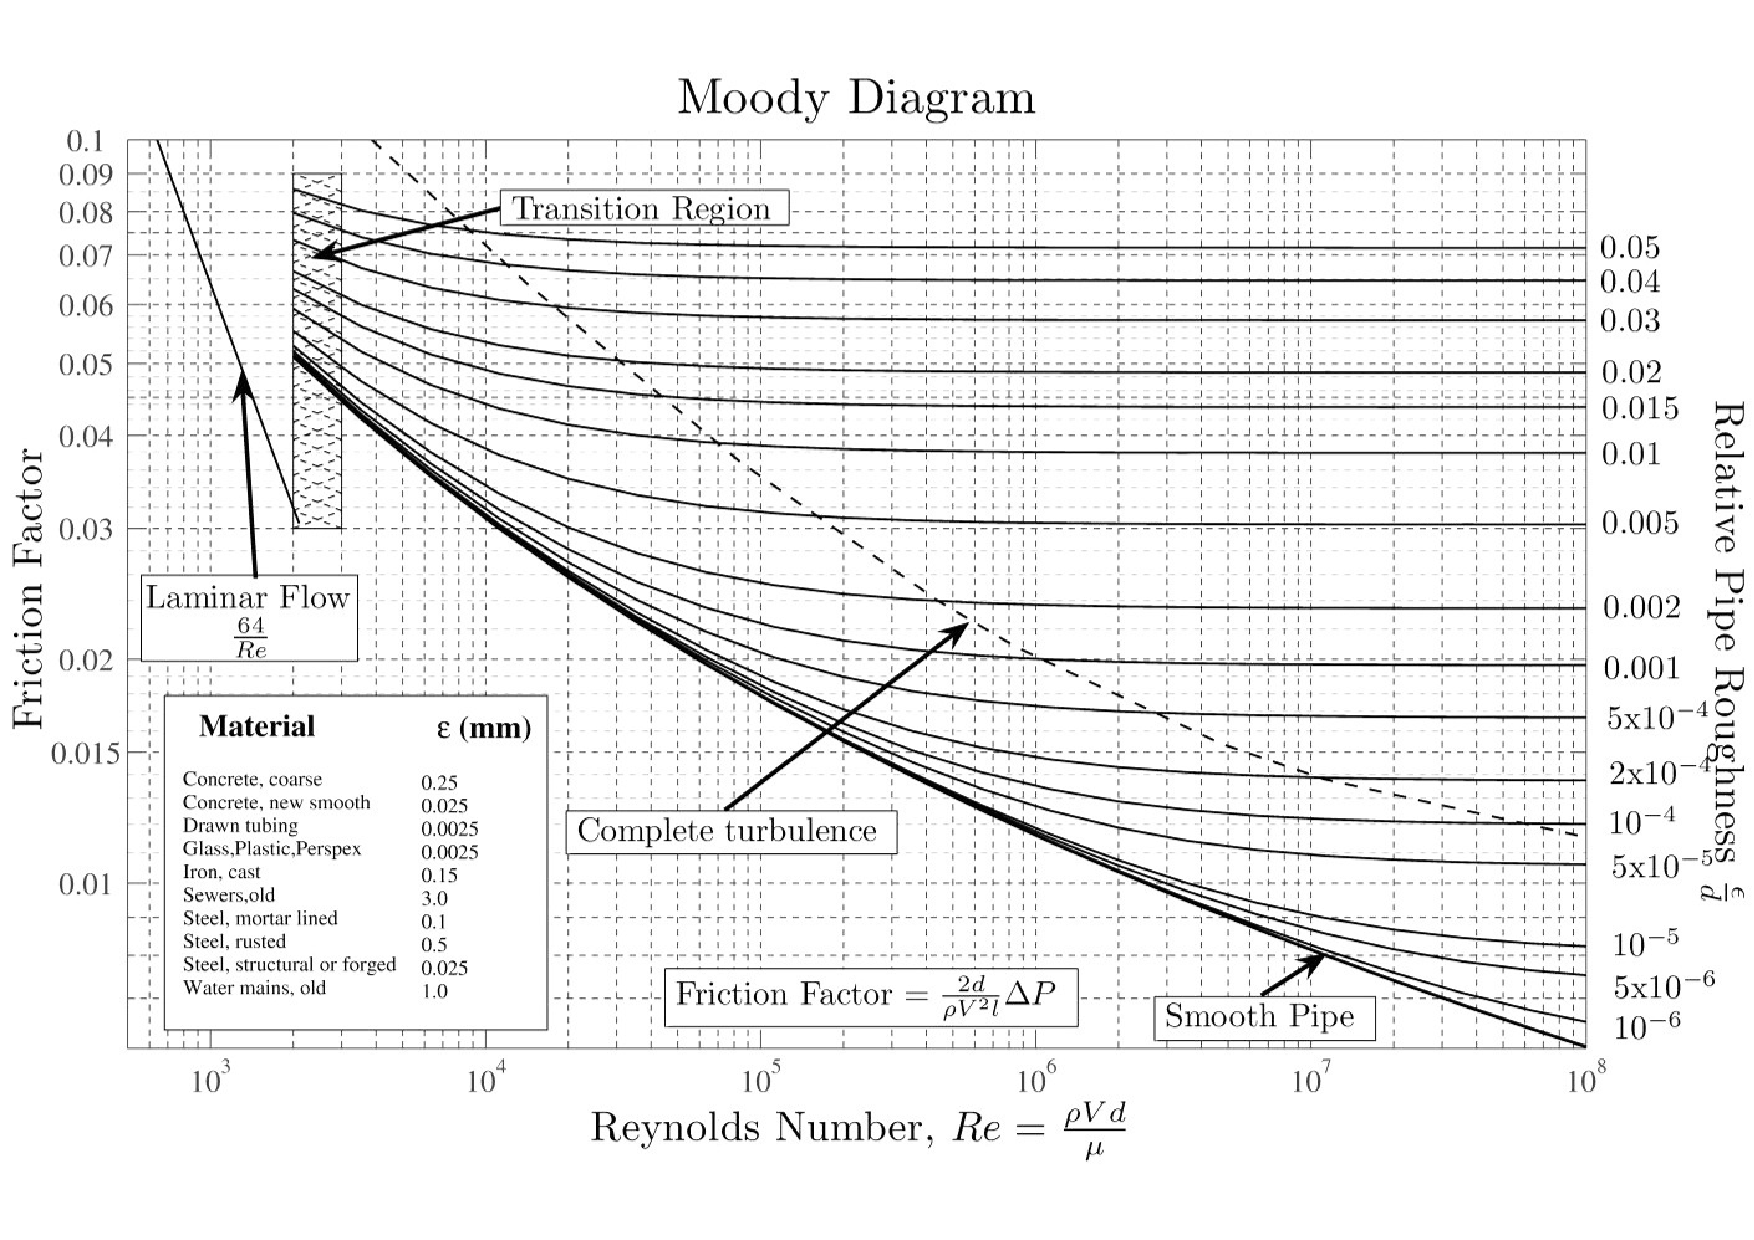
\includegraphics[width=0.85\columnwidth]{images/Moody_chart.pdf}
\caption{Moody friction factor chart. Source: \cite{Moody2008}.}
\label{fig:Moody_chart}
\end{figure}

\begin{table}
\begin{scriptsize}
\caption{Reynold's number (Re) ranges of different flow patterns. Data from McAllister \cite{Mcallister2009}.}
\label{tab:NRe_ranges}
\begin{tabular*}{0.75\columnwidth}{p{0.4\columnwidth}p{0.35\columnwidth}}
\toprule
Flow pattern & NRe [-] \\
\midrule
Laminar flow & Re$<$2000 \\
Transition flow & 2000$\leq$Re$\leq$4000 \\
Turbulent flow & Re$>$ 4000 \\
\bottomrule
\end{tabular*}
\end{scriptsize}
\end{table}

The pipeline flow velocity is calculated as:
%%%%%%%%%%
\begin{equation} \label{eq:flow_velocity}
v_{l,W}=\frac{Q_{l,W}}{A_{P}} \begin{footnotesize} \quad\quad\text{[ft/s]} \end{footnotesize}
\end{equation}
%%%%%%%%%%
where $Q_{l,W}$ = wellbore flow rate or liquid production per well [\unitfrac{ft$^3$}{s}]; and \newline $A_{P}$ = the cross sectional area of the pipe [\unit{ft$^2$}]. The wellbore flow rate is calculated as: 
%%%%%%%%%%
\begin{equation} \label{eq:well_flow_rate}
Q_{l,W} = \frac{Q_{l}}{N_{W}} \begin{footnotesize} \quad\quad[\text{ft}^3/\text{s}] \end{footnotesize}
\end{equation}
%%%%%%%%%%
where $Q_{l}$ = total rate of liquid production [\unitfrac{ft$^3$}{s}]; and $N_{W}$ = number of producing wells. The total rate of liquid production is calculated as: 
%%%%%%%%%%
\begin{equation} \label{eq:total_flow_rate}
Q_{l}=Q_{o} (1+ \text{WOR}) \begin{footnotesize} \quad\quad[\text{ft}^3/\text{s}] \end{footnotesize}
\end{equation}
%%%%%%%%%%
where $Q_{o}$ = total rate of oil production [\unitfrac{bbl}{d}]; WOR= water-to-oil ratio [\unitfrac{bbl}{bbl}]. The total rate of liquid production is converted from [\unitfrac{bbl}{d}] to [\unitfrac{ft$^3$}{s}]. 

The pressure traverse is estimated using the total head as \cite[Table 1, p. 455]{Mcallister2009}:
%%%%%%%%%%
\begin{equation} \label{eq:pressure_traverse}
p_{trav,tot} = 0.43 h_{tot} \gamma_{l} \begin{footnotesize} \quad\quad\text{[psi]} \end{footnotesize}
\end{equation}
%%%%%%%%%%
where $p_{trav,tot}$ = total pressure traverse [psi]; 0.43 = fresh water gradient at 60 $^{\circ}${F} [psi/ft] \cite[p. 25]{Rose1989}; $h_{tav,tot}$ = total head [ft]; and $\gamma_{l}$ = the specific gravity of the crude oil mixture [-], calculated as:
%%%%%%%%%%
\begin{equation} \label{eq:mixture_gravity}
\gamma_{l}= \gamma_{o}\lambda _{o} + \gamma_{w} \lambda _{w} \begin{footnotesize} \quad\quad\text{[-]} \end{footnotesize}
\end{equation}
%%%%%%%%%%
where $\gamma_{o}$ = the specific gravity of oil [-]; $\gamma_{w}$ = the specific gravity of water [-]; $\lambda _{o}$ = fraction of oil [fraction]; and $\lambda _{w}$ = fraction of water [fraction]. The fraction of oil is calculated as:
%%%%%%%%%%
\begin{equation} \label{eq:oil_fraction}
\lambda _{o}= \frac{Q_{o}}{Q_{o}(1+\text{WOR})} \begin{footnotesize} \quad\quad\text{[-]} \end{footnotesize}
\end{equation}
%%%%%%%%%%
The elevation component of the pressure traverse is estimated using a linear one phase flow model where the gas-to-liquid ratio is equal to zero (GLR= 0) and the temperature and pressure effects are ignored. Figure\,\ref{fig:phase_comparison} shows an example of a linear pressure-traverse curve for a particular production rate and fluid properties. The slope of the curve is the relative density of the flowing oil-water mixture. For GLR$>$0 the relationship becomes non-linear and the pressure traverse becomes less sensitive to changes in the well depth with increasing GLR \cite[p. 27]{Clegg2007}. However, the generation of a non-linear relationship requires the application of the multi-phase flow correlations which requires an iterative, trial-and-error solution to account for the changes in flow parameters as a function of pressure. Due to the complexity of this approach, we do not implement multi-phase flow in OPGEE \version. 

\begin{figure}[t]
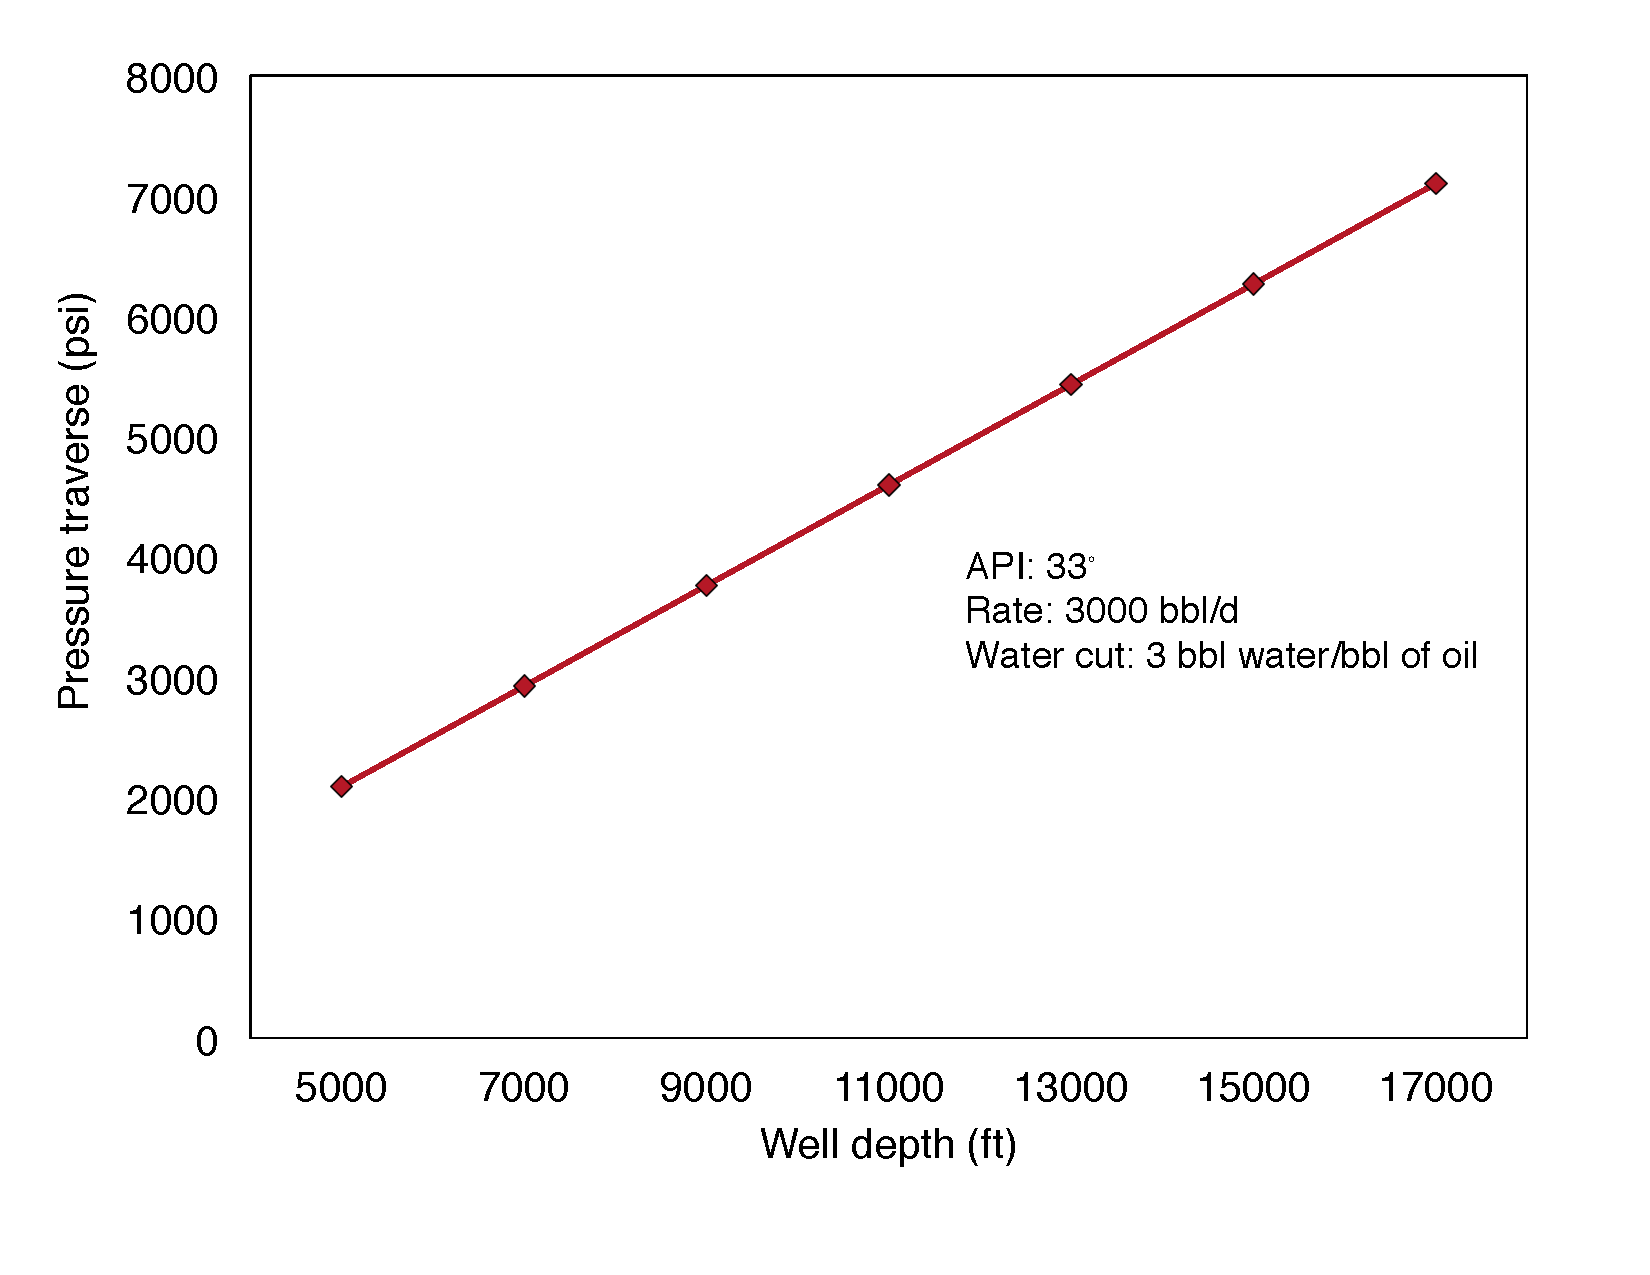
\includegraphics[width=0.8\columnwidth]{images/phase_flow_study.pdf}
\caption{An example of a linear pressure traverse curve (GLR= 0).}
\label{fig:phase_comparison}
\end{figure}

\subsubsection{Pressure for lifting}

The second step after estimating pressure traverse is the calculation of the pressure for lifting which is the pressure required by artificial means (e.g., pump) to lift the oil-water mixture to the surface at the desired wellhead pressure. The pressure for lifting is calculated as: \marginnote{Production \& Extraction 2.2.2} 
%%%%%%%%%%
\begin{equation} \label{eq:pressure_lifting}
p_{lift}=(p_{trav,tot}+p_{wh})-p_{wf} \begin{footnotesize} \quad\quad\text{[psi]} \end{footnotesize}
\end{equation}
%%%%%%%%%%
where $p_{lift}$ = pressure for lifting [psi]; $p_{tav,tot}$ = total pressure traverse [psi]; $p_{wh}$ = wellhead pressure [psi]; and $p_{wf}$ = bottomhole pressure [psi]. The wellbore pressure is calculated from the average reservoir pressure by subtracting the pressure drawdown. The pressure drawdown is the difference between the reservoir pressure and the bottomhole pressure \cite[p. 22]{Takacs2005}.

\subsubsection{Pump brake horsepower}

The brake horsepower (BHP) is calculated using the pump discharge flow rate and the pumping pressure as \cite[p. 27]{Rose1989}: \marginnote{Production \& Extraction 2.2.3} 
%%%%%%%%%%
\begin{equation} \label{eq:pump_BHP}
\begin{split}
&\text{BHP$_{P}$}=\frac{1.701 \times 10^{-5} Q_{d} \Delta p}{\eta_P} \begin{footnotesize} \quad\quad\text{[hp]} \end{footnotesize}\\
&\text{This is equivalently expressed as:}\\
&\text{BHP$_{P}$ [hp]}=\frac{\frac{1 [\text{hp}]}{1714 [\text{gpm-psi}]} \frac{42\left[\frac{\text{gal}}{\text{bbl}}\right]}{24\left[\frac{\text{hr}}{\text{d}}\right] 60\left[\frac{\text{min}}{\text{hr}}\right]} Q_{d} \left[\frac{\text{bbl}}{\text{d}}\right] \Delta p [\text{psi}]}{\eta_P} 
\end{split}
\end{equation}
%%%%%%%%%%
where BHP$_{P}$ = brake horsepower [hp]; $Q_{d}$ = pump discharge rate [bbl/d]; \newline $\Delta p$ = pumping pressure [psi]; and $\eta_P$ = pump efficiency [\%]. The term 1714 is a dimensionless factor that converts between [hp] and [gpm-psi]. The pumping pressure is the difference between pump discharge and suction pressures. The default suction pressure is 0 psi. In the case of a downhole pump the pumping pressure is equal to the pressure for lifting as calculated in eq.\ \eqref{eq:pressure_lifting}. 


\clearpage

%%%%%%%%%%%%%%%%%%%%%%%%%%%%%%
\section{Bitumen mining}
\label{sec:bitumen_mining}

Bitumen mining takes in raw bitumen ore (containing sand, bitumen, and water) and produces cleaned and separated bitumen ready for upgrading or dilution.

The streams flowing into and out of the bitumen mining process are shown in Figure \ref{fig:mining_PF} and are listed in Table \ref{tab:mining_PF}.


\clearpage

%%%%%%%%%%%
\begin{table}
\caption{Streams flowing into and out of the bitumen mining process. I/O denotes input or output stream}
\label{tab:mining_PF}
\begin{scriptsize}
\begin{tabularx}{1\columnwidth}{p{0.32\columnwidth}p{0.05\columnwidth}p{0.04\columnwidth}p{0.32\columnwidth}p{0.05\columnwidth}p{0.05\columnwidth}}
\toprule
Flow name							& Stream   			& I/O 	& Source/Destination       			& Units 			&  Notes\\ 
\midrule
Bitumen at mine						& \stream{2}			& I		& Bitumen mine				& [t/d]			&			\\
Fuel gas - Mining						& \stream{167}			& I		& Fuel gas system				& [t/d]			&			\\
Electricity - Mining						& \stream{193}			& I		& Electricity generation and imports	& [MWh/d]			& 			\\
\midrule
Bitumen from mine to upgrader				& \stream{5}			& O		& Separation					& [t/d]			&			\\
Bitumen from mine to dilution				& \stream{6}			& O		& Separation					& [t/d]			&			\\
Mine offgas to flare						& \stream{84}			& O		& Environment - Atmosphere		& [t/d]			&			\\
Mine face fugitives and tailings pond emissions			& \stream{281}			& O	& Environment - Atmosphere		& [t/d]			&			\\	
\bottomrule
\end{tabularx}
\end{scriptsize}
\end{table}
%%%%%%%%%%%


%%%%%%%%%%%
\begin{figure}
\includegraphics[width=0.85\columnwidth]{images/Bitumen_mining_PF.pdf}
\caption{Streams flowing into and out of the bitumen mining process. All streams measured in tonnes per day excepting electricity which is measured in MWh/d.}
\label{fig:mining_PF}
\end{figure}
%%%%%%%%%%%


%%%%%%%%%%%
\begin{table}
\caption{Secondary parameter inputs to the bitumen mining worksheet}
\label{tab:bitumen_mining_SI}
\begin{scriptsize}
\begin{tabularx}{1\columnwidth}{p{0.5\columnwidth}p{0.05\columnwidth}p{0.1\columnwidth}p{0.1\columnwidth}p{0.05\columnwidth}}
\toprule
Parameter name						& Default value   		& Units 	& Source			      			& Notes 		\\ 
\midrule
Mined bitumen temperature	 			& 80					& [$^\circ$F]	& Assumption				& -			\\
Mined bitumen pressure					& 14.7				& [psi] 		& Assumption				& -			\\
Mined bitumen API gravity					& 8					& [$^\circ$API]	& Assumption				& -			\\
Fraction of gas consumed in equip			& [0-1]				& [-]			& Assumption				& -			\\
\bottomrule
\end{tabularx}
\end{scriptsize}
\end{table}
%%%%%%%%%%%


\clearpage


There are seven mining projects currently operating in the Canadian oil sands as of late 2015. The characteristics of each mining operation are summarized in Table \ref{tab:mining_projects}. One of the main differences between oil sands mines is the bitumen froth treatment technology used. Once oil sands material is mined it is transported to a separation facility where hot water is added to produce an oil sands slurry. The slurry is brought to an extraction facility where gravity drainage is used to remove larger solids and produce a bitumen froth, a mixture of bitumen, fine solids, and water. This bitumen froth undergoes froth treatment, in which a light hydrocarbon (either naphthenes or paraffins) acts as a solvent and separates bitumen from other material contained in the bitumen froth.  Older projects (those constructed prior to 2002) all employ naphthenic froth treatment (NFT), while projects constructed from 2002 onwards (with the exception of the CNRL Horizon project which employs NFT) employ paraffinic froth treatment (PFT).  

The bitumen produced at NFT facilities is of lower quality, containing a higher percentage of asphaltenes and more residual water and solids. Bitumen produced at NFT mines must therefore go through upgrading to synthetic crude oil (SCO) and cannot be diluted and sent directly to refineries, as is the case for bitumen produced at PFT facilities. Generally NFT mines include an upgrader located at the mine site. Because natural gas and electricity consumed for the mine and the upgrader are delivered to the site altogether, the facilities share a common cogeneration system and a significant amount of waste heat from the upgrader is used in the bitumen separation process. 

Disentangling use by mining operations alone is challenging given the complex nature of operations. Importantly, the Alberta Energy Regulator (AER) reports natural gas and electricity consumption for integrated mining and upgrading facilities together without specifying the quantities of natural gas and electricity consumed for mining alone. The exception to this is the Syncrude Aurora (NFT) project, as bitumen produced at that site is transported to the Syncrude Mildred Lake (NFT) project for upgrading at the Mildred Lake upgrading facility.  Also, the Suncor upgrader located at the mine site also upgrades bitumen produced at Suncor's Firebag in situ project.  Bitumen produced by the stand-alone Shell Muskeg River and Jackpine (PFT) mines is upgraded at the stand-alone Shell Scotford upgrader, however as the upgrader is located off-site the energy consumption for the mines is reported separately from the upgrading process. The Imperial Kearl project is the only mining project that produces diluted bitumen (known as dilbit) that is sent directly to refineries without undergoing any intermediate upgrading.  Of all the mining projects, the Suncor upgrader produces some diesel fuel that is combusted as a fuel on-site.

\begin{table}
\caption{Characteristics of operating mining projects}
\label{tab:bitumen_mining_data}
\begin{scriptsize}
\begin{tabularx}{1\columnwidth}{p{0.2\columnwidth}p{0.05\columnwidth}p{0.05\columnwidth}p{0.05\columnwidth}p{0.05\columnwidth}p{0.4\columnwidth}}
\toprule
Mine						& Year & Cap. (bbl/d) & Sep. & Int. upgr.? & Notes \\
\midrule
Suncor					& 1967	& 490,000		& NFT	& Yes	&Upgrader also processes bitumen produced from Suncor Firebag in situ project. \\
Syncrude Mildred Lake		& 1978	& 150,000		& NFT	&Yes		& Upgrader also processes bitumen produced at Syncrude Aurora mine. \\
Syncrude Aurora			& 2001	& 200,000		& NFT	& No		& Waste heat from Syncrude Mildred Lake upgrader used in Syncrude Aurora mine. \\
CNRL Horizon				& 2008	& 250,000		& NFT	& Yes	& \\				
Shell Muskeg River			&2002	& 155,000		& PFT	& No		& Bitumen transported to stand-alone Shell Scotford upgrader. \\
Shell Jackpine				& 2010	& 100,000		& PFT	& No		& Bitumen transported to stand-alone Shell Scotford upgrader. \\
Imperial Kearl				& 2013	& 220,000		& PFT	& No		& Only mine that produces diluted bitumen. \\
\bottomrule
\end{tabularx}
\end{scriptsize}
\end{table}

\paragraph{Public Data Available}

Data are available from a number of public sources.  First, the AER publishes monthly Statistical Reports on oil sands operations. Most useful are ST39: \emph{Alberta Mineable Oil Sands Plant Statistics}, which was published from 1970-2002 and 2008-2014 \cite{AERvar}; as well as ST43: \emph{Alberta Oil Mineable Oil Sands Plant Statistics - Annual}, which was published in years 2003-2007 \cite{AERvarSt43}. These statistical reports tabulate monthly energy consumption, flared/wasted fuels, and electricity, bitumen, and SCO production for each oil sands project. Some projects operated by the same company receive fuel at one mine and then deliver fuel to the other mine and so report the total fuel consumption under the mine that receives the fuel (e.g., Syncrude's Mildred Lake and Aurora projects) rather than reporting the fuel consumption for each project separately \cite{AER2016}.
 
Definitions provided by AER for energy consumption reported in the AER's ST39 and ST43 reports include definitions of some potentially ambiguous data \cite{AER2016}:
\begin{itemize}
\item SCO Fuel Use: The total volume of SCO combusted as fuel at the facility.
\item SCO Plant Use: The total volume of SCO used at the facility for uses other than fuel.
\item Bitumen Flared/Wasted: The total volume of unrecovered crude bitumen from spills, upgrading slops, tanks dewatering etc.
\end{itemize}
Note that diesel fuel consumption for each project is collected by the AER but not reported in any of the AER's reports \cite{AER2016}. One project, Suncor, does report that the upgrader produces diesel fuel that is used as fuel on site for mining operations. This use is reported under the AER as SCO fuel consumption \cite{AERvar}.

Another important data source are engineering ``templates'' generated by the Canada's Oil Sands Innovation Alliance (COSIA). COSIA has published two mine templates that contain material and energy flow diagrams for the two froth treatment technologies (naphthenic froth treatment and paraffinic froth treatment) employed in the oil sands \cite{COSIA2015a, COSIA2015b}. For each froth treatment technology, energy and material flows are presented for two possible oil sands ore qualities: low grade ore at 9 wt.\% bitumen, and high grade ore at 12 wt.\%. The COSIA Mine Templates provide approximate energy consumption values for a representative mining project based on existing oil sands operations but not representative of any currently operating oil sands project.

A last source of data is the Alberta Environmental Monitoring, Evaluation, and Reporting Agency (AEMERA), which has published estimates of fugitive GHG emissions from mine face, tailings ponds, and `other' (e.g., emissions from pipe fitting and equipment leaks, releases from pressure relief valves, tanks, and sewage lagoons) for each oil sands company operating a mining project from January 1st, 2011 to December 31st, 2014 \cite{AEMERA2015}. The fugitive GHG emissions generated by AEMERA are developed from figures reported by companies to the Government of Alberta under the Specified Gas Emitters Regulation (AB, 2007). The estimated fugitive CH$_4$ emissions from oil sands mine face and tailings ponds reported by AEMERA are close to the numbers reported elsewhere \cite{Johnson2016, GHGenius4.03}.

In order to capture the range of mining projects, OPGEE models two template mining operations: 
\begin{itemize}
\item an upgrader-integrated mine using naphthenic froth treatment (NFT) separation technology;
\item A stand-alone mine using paraffinic froth treatment (PFT) separation technology.
\end{itemize}

As can be seen in Table \ref{tab:mining_projects} above, the integrated mine and upgrader using NPT separation is more indicative of older large-scale mining projects developed in the 1970s and 1980s, such as the Suncor and Syncrude operations.  Additionally, the more recently developed CNRL Horizon project is an integrated NFT mine.  The non-integrated mine with PFT separation is more representative of modern developments such as Albian Sands (Shell), Aurora (Syncrude), Jackpine (Shell), and Kearl (Imperial). 

Public natural gas and electricity consumption literature data available, AER facility-reported data and COSIA Mine Template ranges, is presented in Figures \ref{fig:mining_ng} and \ref{fig:mining_elec}, respectively, below. Production-weighted average energy consumption is reported for both 2014 and over the project life based on the AER data reported for each facility. The shaded regions represent the natural gas consumption for NFT and PFT mines presented in the COSIA Mine Template for low grade and high grade ore. Note that no corresponding graph can be created for diesel consumption due to lack of consistent reporting of diesel use in AER datasets.

There is some challenge in interpreting reported public data. First, note that natural gas consumption reported by AER for Suncor, Syncrude Mildred Lake, and CNRL Horizon mines includes natural gas consumed in on-site upgraders. Similarly, electricity consumption reported by AER for Suncor, Syncrude Mildred Lake, and CNRL Horizon mines include electricity consumed in on-site upgraders. Lastly, the Shell Muskeg River mine receives the majority of natural gas that is consumed at Shell Jackpine mine, meaning that per-mine consumption at each Shell mine is between the two reported values (high for Muskeg River and very low for Jackpine).  The separation of stand-alone vs.\ integrated upgrading mines, is discussed more fully below.


\begin{figure}[t]
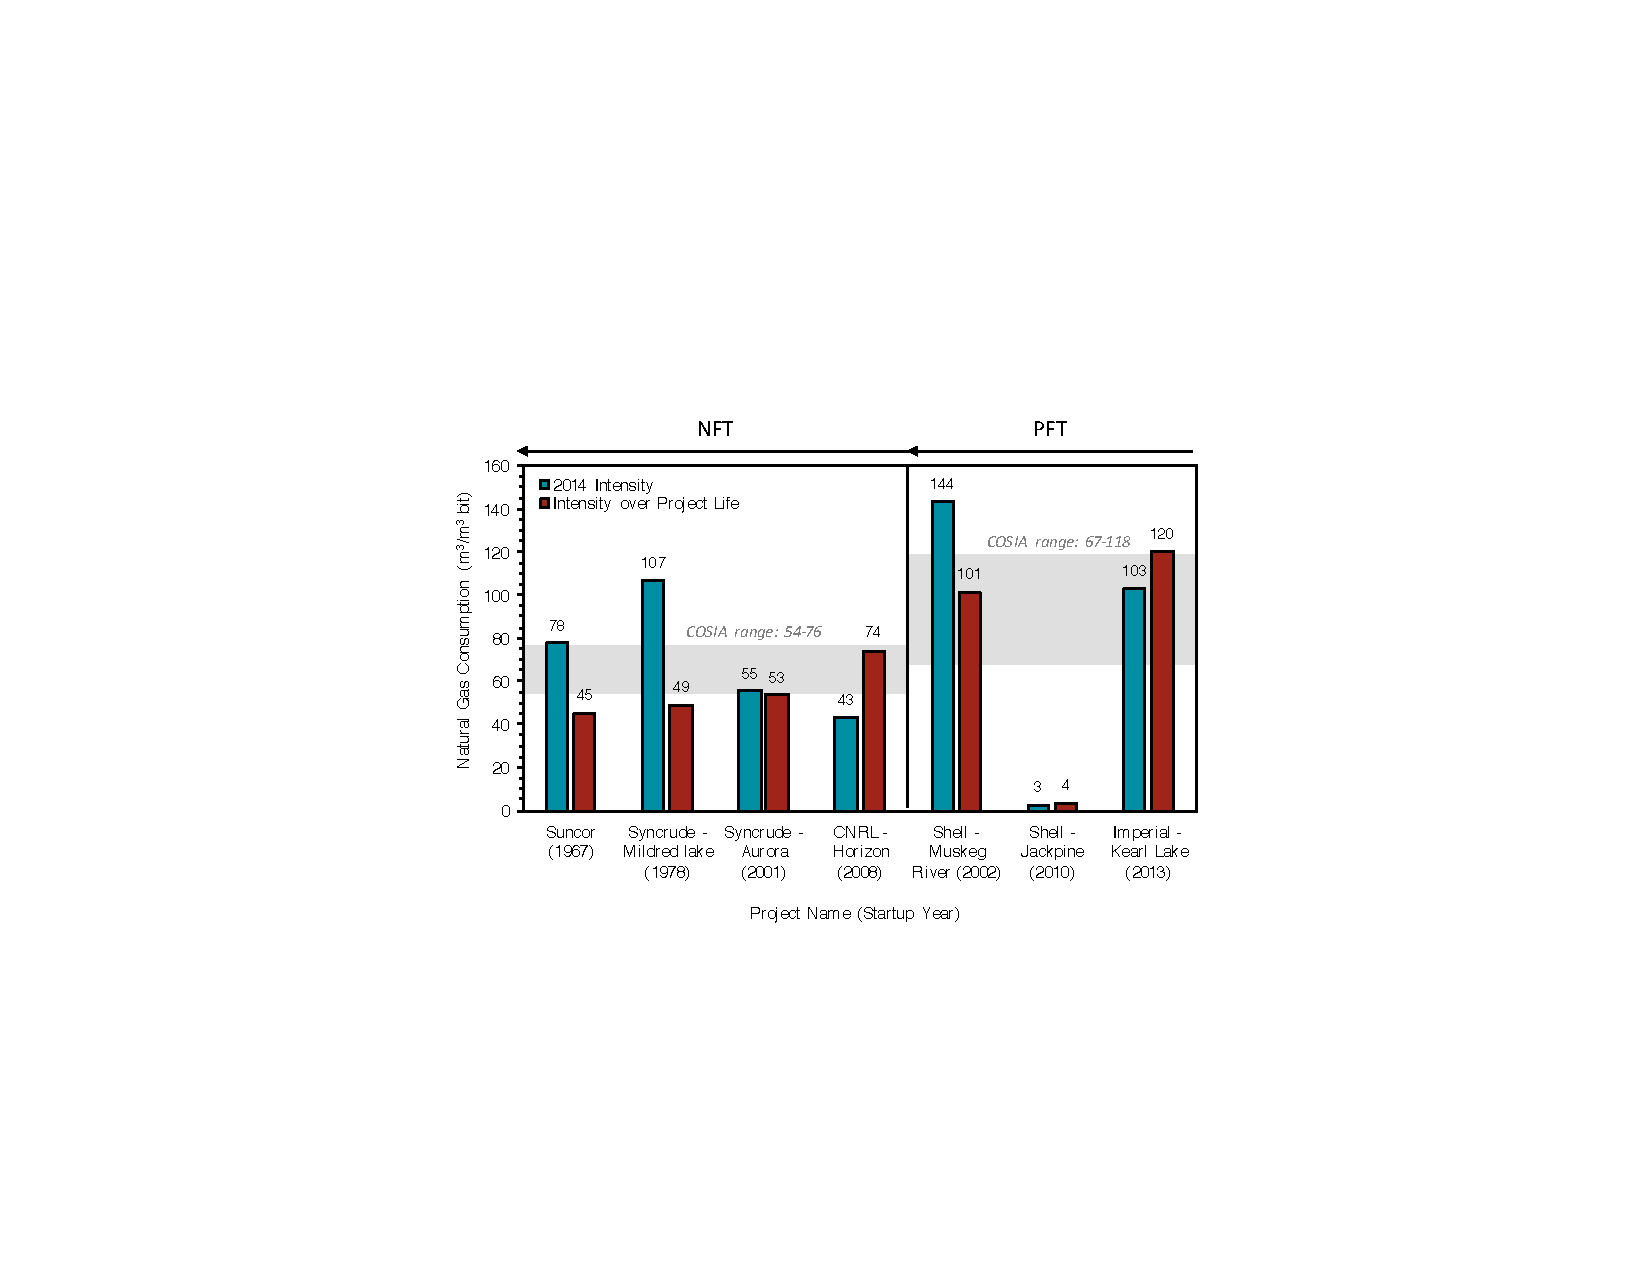
\includegraphics[width=1\columnwidth]{images/mining_ng.pdf}
\caption{Natural gas use in mining operations}
\label{fig:mining_ng}
\end{figure}


\begin{figure}[t]
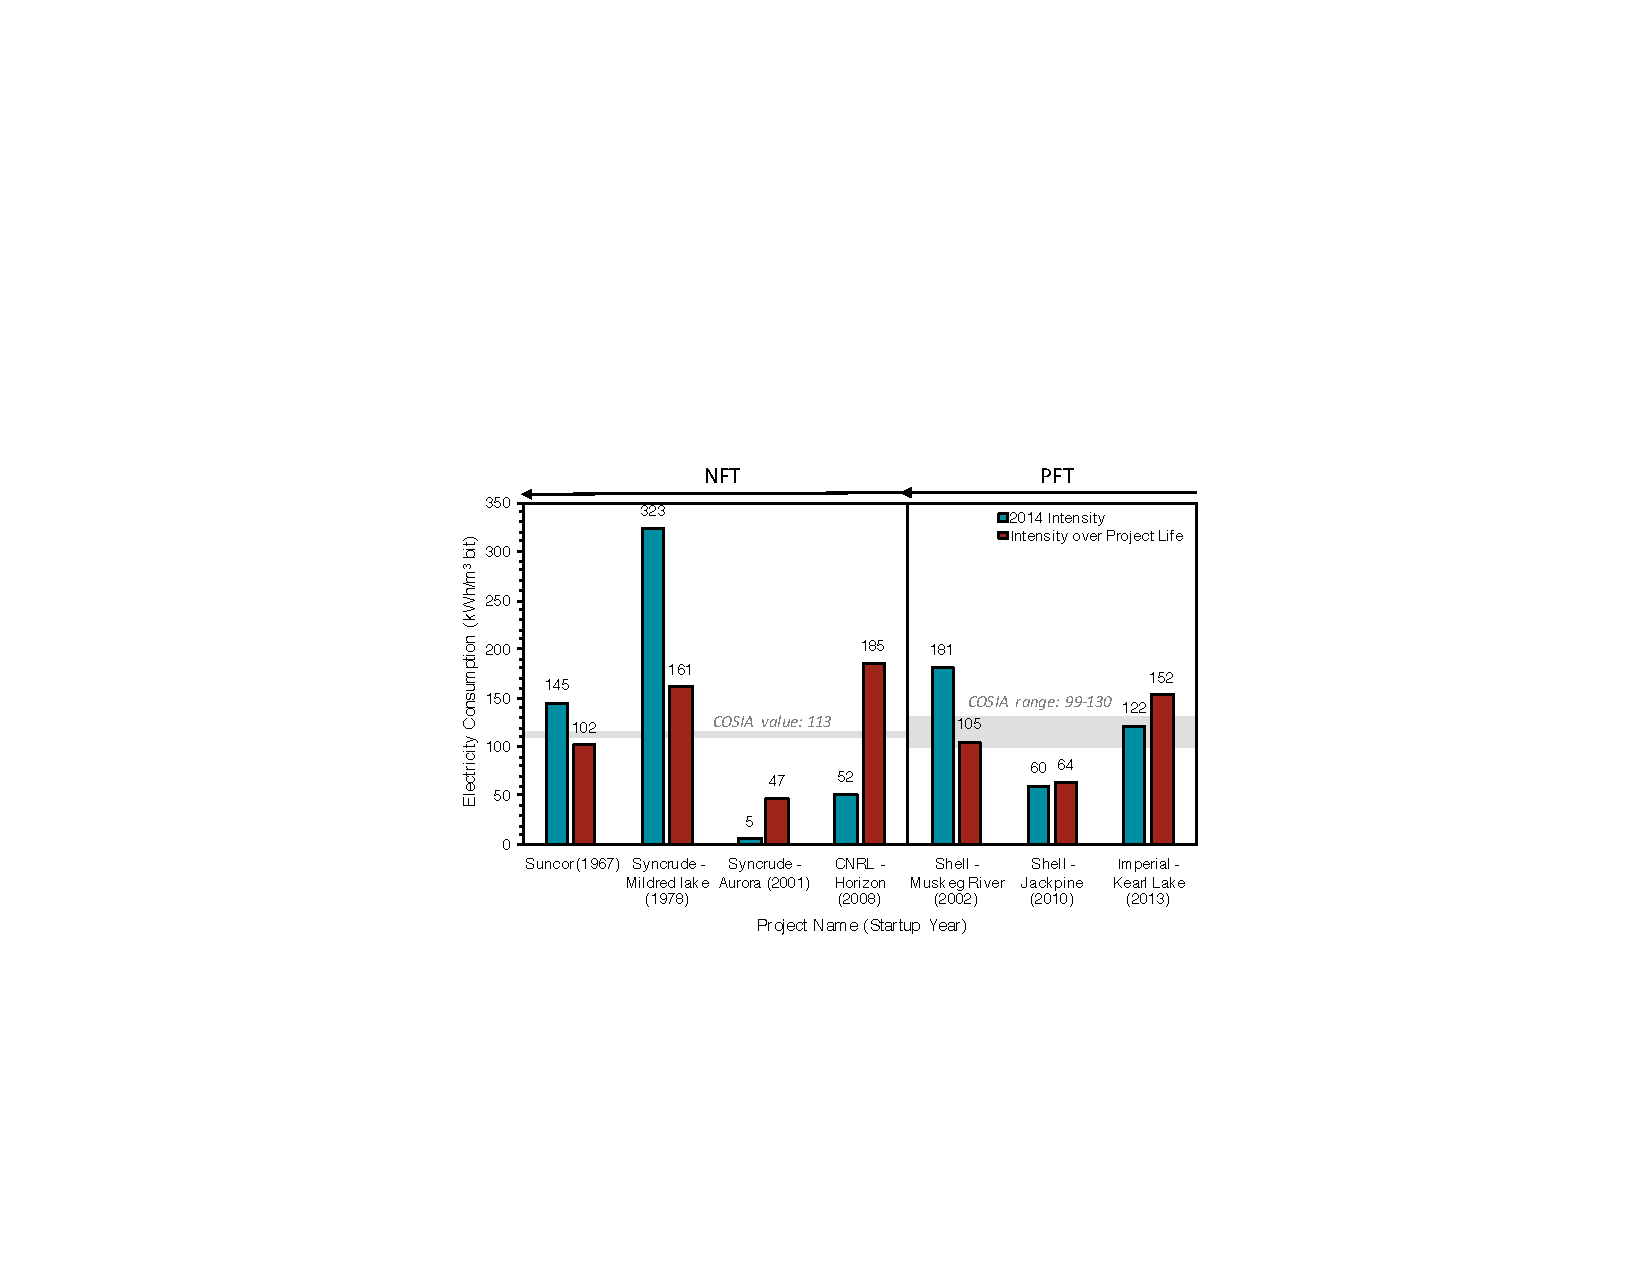
\includegraphics[width=1\columnwidth]{images/mining_elec.pdf}
\caption{Electricity use in mining operations}
\label{fig:mining_elec}
\end{figure}

\paragraph{Modeling of non-integrated PFT mining operations}

The non-integrated mining operation is illustrated in Figure \ref{fig:pfd_mining_nint}.  The energy imports to the stand-alone mining operation include diesel imports, electricity imports, and natural gas imports. Some mining operations co-generate power on site and may also export power. The mine takes in raw bitumen ore and exports diluted bitumen for shipment to upgraders or direct shipment to refineries.

The default values for energy use in non-integrated PFT mining operations are computed as follows:
\begin{itemize}
\item Natural gas consumption is modeled using the AER 2014 production-weighted average for three stand-alone PFT projects (Shell Muskeg River, Shell Jackpine, and Imperial Kearl).
\item Electricity consumption is modeled using the AER 2014 production-weighted average for three stand-alone PFT projects (Shell Muskeg River, Shell Jackpine, and Imperial Kearl).
\item Diesel consumption is estimated as the average of COSIA reported high and low ranges of diesel consumption, as reported for low-grade (9 wt.\% and high-grade (12 wt.\%) ores respectively. The range from the COSIA templates is used as the range of diesel consumption rate.
\item Diluent blending rates are modeled using AER 2014 production-weighted averages from the stand-alone PFT projects (Shell Muskeg River, Shell Jackpine, and Imperial Kearl). Volumetric blending rates over all months averaged 25.4\% diluent in dilbit. The range over 2014 was from 24.3\% to 26.5\% Although Kearl dilutes bitumen with SCO (creating ``syn-bit'') the dilution fraction was nearly identical to those of Muskeg River and Jackpine.
\end{itemize}

Table \ref{tab:mining_nonint_energy} gives results as used in OPGEE, results for the AER production-weighted average, COSIA template average, and COSIA template range.


\begin{table}
\begin{scriptsize}
\tablefirsthead{\toprule Fuel & OPGEE value & AER PW avg. & COSIA avg. & COSIA range & Notes\\
\midrule}
\tablehead{ \multicolumn{6}{p{1\columnwidth}}{\textit{Continued from previous page}}\\ \toprule Fuel & AER prod-weighted avg. & COSIA avg. & COSIA range & Notes \\ 
\midrule }
\tabletail{\bottomrule \multicolumn{6}{p{1\columnwidth}}{\textit{Continued on next page...}}\\}
\tablelasttail{\bottomrule}
\tablecaption{Non-integrated PFT mining energy intensities}
\label{tab:mining_nonint_energy}
\begin{threeparttable}
\begin{supertabular*}{1\columnwidth}{p{0.2\columnwidth}p{0.1\columnwidth}p{0.1\columnwidth}p{0.1\columnwidth}p{0.1\columnwidth} p{0.1\columnwidth}}
		
Natural gas		& 85		& 85		& 93		& 67 -- 118 		& \\
Electricity	cons.	& 125	& 125	& 114	& 99 -- 130		& \\
Electricity gen.		& 77		& 77		& 114	& 96 -- 132		& \\
Frac. elect. gen. onsite	& 0.6 	& 0.6		& 1.0		& 1.0 -- 1.0	& \\
Diesel			& 12.5	& -		& 12.5	& 9 -- 16			& a \\	
Diluent			& 25.4\%	& 25.4\%	& -		& -				& \\
\end{supertabular*}
\begin{tablenotes}
\item[a] COSIA Mine Template ranges presented for low (9\%) and high (12\%) grade ore.
\end{tablenotes}
\end{threeparttable}
\end{scriptsize}
\end{table}



\paragraph{Proposed modeling of integrated NFT mining operations}


The integrated mining operation is illustrated in Figure \ref{fig:pfd_mining_int}.  The net flows across the process boundary are roughly equivalent to the stand-alone mining operation, with some exceptions. First, large volumes of diluent are not used to reduce the viscosity of bitumen, as upgrading the bitumen to SCO renders it ready for pipeline transport.  Also, two new co-products can be exported from the system: process gas and coke.  Therefore, emissions credits should be given for these fuels if they are exported.  Lastly, new internal flows between upgrader and mine include heat recovered from upgrader operations that is used in mine ore separations, as well as upgrader product streams (distillate fuels) that are consumed in mining trucks.  New internal consumption at the upgrader can include coke and process gas.

Due to sharing of waste heat at integrated mining and upgrading projects, some efficiency is gained through process integration.  Suncor and Jacobs (2012) estimate that 30 percent of total natural gas required at a project can be reduced by using low-grade waste heat from an integrated upgrader for the bitumen extraction process.

Updated OPGEE default values for stand-alone NFT mines are taken directly from the COSIA NFT Mine Template \cite{COSIA2015b}. The efficiency factor from Suncor and Jacobs \cite{Jacobs2012} is multiplied by the COSIA stand-alone mining natural gas consumption to approximate the natural gas consumed solely by the mine at an integrated mining and upgrading facility. These values are compared to the energy consumption for integrated mining and upgrading projects in Table \ref{tab:mining_comp_integration}. The remaining energy for integrated projects not attributed to mining is approximately that consumed in the upgrading process.  For example, if we compare Suncor and Syncrude natural gas consumption (total) less that estimated used in upgrading, we get values approximately equalto the COSIA stand-alone NFT mine less a 30\% integration benefit (40-45 m$^3$ per $m^3$) .  

\begin{landscape}
\begin{table}
\begin{scriptsize}
\tablefirsthead{\toprule Fuel & OPGEE value$^{a}$ & COSIA SA NFT$^{b}$ & AER reported$^{c}$ & & Upgrading est.$^{d}$ & \\ \midrule}
\tabletail{\bottomrule \multicolumn{7}{p{1\columnwidth}}{\textit{Continued on next page...}}\\}
\tablelasttail{\bottomrule}
\tablecaption{Comparison between stand-alone mine energy consumption estimates based on COSIA mine template to integrated NFT mining and upgrading energy consumption reported by AER}
\label{tab:mining_comp_integration}
\begin{threeparttable}
\begin{supertabular*}{1\columnwidth}{p{0.2\columnwidth}p{0.1\columnwidth}p{0.1\columnwidth}p{0.1\columnwidth}p{0.1\columnwidth} p{0.1\columnwidth}p{0.1\columnwidth}}
				&		&				& Suncor	& Syncrude	& Suncor	& Syncrude \\	
				\midrule
Natural gas cons.	& 45		& 65 (54 -- 76)		& 78		& 77			&	30 	& 37  \\
Electricity	cons.	& 113	& 113			& 145	& 166		& 	30	& 63 \\
\end{supertabular*}
\begin{tablenotes}
\item[a] Natural gas consumption for mining portion of an integrated mining and upgrading project calculated by subtracting the percentage of natural gas Suncor and Jacobs \cite{Jacobs2012} estimate will be saved through sharing of waste heat. 
\item[b] Includes mining energy consumption estimates provided in COSIA Mine Templates for a representative stand-alone NFT mine.
\item[c] 2014 operating data reported in AER Statistical Report ST39. Suncor and Syncrude projects have on-site upgraders so AER data is reported for both mining and upgrading.
\item[d] Estimate of energy consumed from upgrading calculated by subtracting the estimated energy consumed for mining in integrated projects from the mining and upgrading energy consumption reported to the AER. The values presented in the table for upgrading are per m$^3$ of SCO produced by the on-site upgrader (17,200,000 m$^3$ and 15,200,000 m$^3$ for Suncor and Syncrude upgraders, respectively), whereas the energy consumption values for mined bitumen presented in the table are per m$^3$ of bitumen produced.
\item[e] The range presented in the table for natural gas consumption from the COSIA Mine Template for NFT projects is based on the low and high estimates for natural gas consumption for high grade and low grade oil sands ore, respectively. The same values for electricity consumption are reported for low and high grade ore in the NFT COSIA Mine Template (113 kWh/m$^3$ bitumen).
\end{tablenotes}
\end{threeparttable}
\end{scriptsize}
\end{table}
\end{landscape}


In order to enable self-consistent treatment of integrated mining and upgrading, the following conventions are applied:
\begin{itemize}
\item Integrated mining and upgrading operations use the same upgrading models described below in Section \ref{sec:upgrading}.
\item Any benefits associated with upgrading integration result in less net consumption of mining consumables that flow across conventional mine boundary (i.e., diesel, electricity, natural gas).
\item Emissions associated with on-site use of fuels by upgrader are calculated on the upgrading sheet.
\end{itemize}
These conventions allow for computation of the benefits of integrated mining and upgrading operations, while also maintaining computations of emissions impacts of operations.

The default values for energy use in upgrader-integrated NFT mining operations are therefore computed as follows:
\begin{itemize}
\item Natural gas consumption is modeled using COSIA stand-alone NFT mine less a 30\% integration benefit. This is approximately equal to the reported values of Suncor and Syncrude less estimated upgrading consumption.
\item Electricity consumption is modeled using COSIA electricity use at a stand-alone NFT mine.  No integration benefit applicable.
\item Diesel consumption is estimated as the average of COSIA reported high and low ranges of diesel consumption, as reported for low-grade (9 wt.\% and high-grade (12 wt.\%) ores respectively.
\end{itemize}



\begin{table}
\begin{scriptsize}
\tablefirsthead{\toprule Fuel & OPGEE value & AER PW avg. & COSIA avg. & COSIA range & Notes\\
\midrule}
\tablehead{ \multicolumn{6}{p{1\columnwidth}}{\textit{Continued from previous page}}\\ \toprule Fuel & AER prod-weighted avg. & COSIA avg. & COSIA range & Notes \\ 
\midrule }
\tabletail{\bottomrule \multicolumn{6}{p{1\columnwidth}}{\textit{Continued on next page...}}\\}
\tablelasttail{\bottomrule}
\tablecaption{Integrated NFT mining energy intensities}
\label{tab:mining_int_energy}
\begin{threeparttable}[t]
\begin{supertabular*}{1\columnwidth}{p{0.2\columnwidth}p{0.1\columnwidth}p{0.1\columnwidth}p{0.1\columnwidth}p{0.1\columnwidth} p{0.1\columnwidth}}
Natural gas		& 45		& -		& 65		& 54 -- 76		& $a$\\
Electricity	cons.	& 113	& -		& 113	& 113 -- 113		& \\
Electricity gen.		& 114	& -		& 114	& 96 -- 132		& \\
Frac. elect. gen. onsite	& 1 	& -		& 1.0 	& 0.8-- 1.2	& \\
Diesel			& 11	& -		& 11	& 9 -- 13			& $b$ \\	
\end{supertabular*}
\begin{tablenotes}
\item[a] Note from Table \ref{tab:mining_comp_integration} above that the COSIA stand-alone NFT mine consumption must be reduced by the heat integration benefit. That is, OPGEE value of 45 m$^3$ per m$^3$ bitumen should be compared to 65$\times (1.0-0.3)$) \cite{COSIA2015b}
\item[b] COSIA Mine Template ranges presented for low (9\%) and high (12\%) grade ore.
\end{tablenotes}
\end{threeparttable}
\end{scriptsize}
\end{table}


\begin{figure}[t]
\includegraphics[width=0.9\columnwidth]{images/mining_nint.pdf}
\caption{Non-integrated bitumen mining operation}
\label{fig:pfd_mining_nint}
\end{figure}


\begin{figure}[t]
\includegraphics[width=1\columnwidth]{images/mining_int.pdf}
\caption{Upgrader-integrated bitumen mining operation}
\label{fig:pfd_mining_int}
\end{figure}

For both integrated and non-integrated mining operations, the emissions and energy use are tracked simply.  For example, diesel fuel use in non-integrated mining operations is computed as:
\begin{equation}\label{eq:dieselmine}
Q_{di}^{MN} = Q_{db}^{MN} I_{di}^{MN}
\end{equation}
where $Q_{di}^{MN}$ is diesel consumed in non-integrated mining operations [gal/d], $Q_{db}^{MN}$ is diluted bitumen output from the non-integrated mining operation [bbl/d], and $I_{di}^{MN}$ is the diesel fuel intensity of non-integrated mining operations [gal/bbl].  This quantity of diesel fuel consumed can then be converted into an energy consumption rate:
\begin{equation}
E_{di}^{MN} = Q_{di}^{MN} LHV_{di}
\end{equation}
where $LHV_{di}$ is the lower heating value of diesel fuel [mBtu LHV/gallon].  This quantity can then be gathered on the \sheet{Energy Consumption} gathering sheet and used to compute emissions on the \sheet{GHG Emissions} gathering sheet.

Similar quantities are computed for all main inputs to non-integrated mining operations by using intensities of electricity use ($I_{el}^{MN}$) and natural gas ($I_{ng}^{MN}$).  For the case of integrated mining and upgrading operations, the relevant intensities for diesel, electricity, and natural gas are similarly named ($I_{di}^{MI}$, $I_{el}^{MI}$, and $I_{ng}^{MI}$ respectively). Recall via convention above that consumption of coke or refinery process gas is computed as part of upgrading operations in Section \ref{sec:upgrading}.

After these mine-type-specific calculations are performed, the overall consumption due to mining is then computed using binary variables from the \sheet{Active Field} sheet. For the case of diesel energy consumption:
\begin{equation}\label{eq:minesum}
E_{di} = y^{MN}E_{di}^{MN}  + y^{MI}E_{di}^{MI}
\end{equation}
where $y^{MN}$ and $y^{MI}$ represent binary variables for mining-non-integrated and mining-integrated, respectively.

\clearpage



%%%%%%%%%%%%%%%%%%%%%%%%%%%%
\section{Separation}
\label{sec:Separation}

The streams flowing into and out of the separation process are shown in Figure \ref{fig:separation_PF} and are listed in Table \ref{tab:separation_PF}.

[TBD: ADD WHOLE SECTION ON SEPARATION, INCLUDING THE COMPRESSION FOR STAGE 2 AND STAGE 3]


\clearpage

%%%%%%%%%%%
\begin{table}
\caption{Streams flowing into and out of the separation process. I/O denotes input or output stream}
\label{tab:separation_PF}
\begin{scriptsize}
\begin{tabularx}{1\columnwidth}{p{0.32\columnwidth}p{0.05\columnwidth}p{0.04\columnwidth}p{0.32\columnwidth}p{0.05\columnwidth}p{0.05\columnwidth}}
\toprule
Flow name							& Stream   			& I/O 	& Source/Destination       			& Units 			&  Notes\\ 
\midrule
Oil at wellhead							& \stream{4}			& I		& Wellbore/downhole pump		& [t/d]			&			\\
Water at wellhead						& \stream{102}			& I		& Wellbore/downhole pump		& [t/d]			&			\\
Gas at wellhead						& \stream{27}			& I		& Wellbore/downhole pump		& [t/d]			&			\\
\midrule
Oil after separator						& \stream{7}			& O		& Crude oil dewatering			& [t/d]			&			\\
Water after separator 					& \stream{103}			& O		& Produced water treatment		& [t/d]			&			\\
Gas after separator						& \stream{28}			& O		& Flaring						& [t/d]			&			\\
Separator leaks to air					& \stream{251}			& O		& Environment - Atmosphere		& [t/d]			&			\\	
\bottomrule
\end{tabularx}
\end{scriptsize}
\end{table}
%%%%%%%%%%%


%%%%%%%%%%%
\begin{figure}
\includegraphics[width=0.85\columnwidth]{images/separation_PF.pdf}
\caption{Streams flowing into and out of the separation process. All streams measured in tonnes per day excepting electricity which is measured in MWh/d.}
\label{fig:separation_PF}
\end{figure}
%%%%%%%%%%%



%%%%%%%%%%%
\begin{table}
\caption{Secondary parameter inputs to the separator worksheet}
\label{tab:separator_SI}
\begin{scriptsize}
\begin{tabularx}{1\columnwidth}{p{0.4\columnwidth}p{0.05\columnwidth}p{0.1\columnwidth}p{0.1\columnwidth}p{0.15\columnwidth}}
\toprule
Parameter name						& Default value   		& Units 	& Source			      							& Notes 		\\ 
\midrule
Amount of water in inlet gas	 			& 52					& [lb/mmscf]	&  \cite[p. 160]{Manning1991}				& -			\\
Entrained water as a fraction of oil emulsion	& 14					& [wt\%]			& \cite{Manning1991}					& -			\\
Number of separator stages				& 3					& [stages] 		& Assumption							& -			\\
Final separator pressure					& 150				& [psi]			& Assumption							& -			\\
Final separator temperature				& 90					& [$^\circ$F]		& Assumption							& -			\\
Separator compressor - Ratio of specific heats	& 1.28				& [-]				& \cite{McAllister2009}					& -			\\
Separator compressor - Compressor eff.		& 0.75				& [\%]			& Assumption							& -			\\
Separator compressor - Prime mover		& 2					& [option]			& Assumption							& 1=e$^-$, 2=NG \\
Wells per separator						& 10					& [wells]			& Assumption							& -			\\
\bottomrule
\end{tabularx}
\end{scriptsize}
\end{table}
%%%%%%%%%%%


\clearpage





%%%%%%%%%%%%%%%%%%%%%%%%%%%%
\section{Heater-treater (dewatering)}
\label{sec:Dewatering}

Removing free water from crude oil can be accomplished by passive chemical and gravitational methods that do not use heat. Because no fuel is used in passive gravitational separation techniques, they do not cause significant GHG emissions. However, based on the properties of the oil, gravity separation techniques may not be sufficient to produce crude oil with the desired water content required for transport and sales. Additional separation may be provided by a crude oil heater-treater, which may be turned ON or OFF in OPGEE, \cellref{Active Field J109} to remove entrained water remaining after passive separation. 

The streams flowing into and out of the \sheet{Heater-Treater} sheet are shown in Figure \ref{fig:crude_oil_dewatering_PF} and are listed in Table \ref{tab:Heater-treater_SI}.

To model heat capacity differences between water and oil \cite[p. 303]{Manning1995}, OPGEE assumes that oil entering a heater-treater contains only entrained water. The free water proportion that was not separated prior to the application of heat is assumed to be negligible (1-2\%)  \cite[Section 5.4.2]{Abdelaal2003}. 

The mass flow of incoming oil and water are given by the constituents of \stream{7} which leaves the separator: $m_{\mstream{7},o}$ and $m_{\mstream{7},w}$. The enthalpy change required is calculated using:
%%%%%%%%%%
\begin{equation} \label{eq:crude_dehyd_heat}
\cellref{M58} \quad \Delta H_{HT}= \Delta T_{HT} \left( m_{\mstream{7},o} C_{p_{o}} + m_{\mstream{7},w} C_{p_{w}} \right) (1+\epsilon_{HT}) \left( \frac{1}{10^6} \right) \eqnunitfrac{MMBtu}{d}
\end{equation}
%%%%%%%%%%
where $\Delta H_{CD}$ = heat duty [MMBtu/d]; $C_{p_{o}}$ = specific heat of oil [Btu/lb-$^{\circ}${F}]; $C_{p_{w}}$ = specific heat of water [Btu/lb-$^{\circ}${F}]; $\Delta T_{HT}$ = difference between treating and feed temperatures, $T_{HT} - T_{\mstream{7}}$ [$^{\circ}${F}]; and $\epsilon_{CD}$ = heat loss [fraction]. 
The specific heat capacity of oil is a function of the temperature of the oil and its API gravity. From the Campbell equation, presented in Manning and Thompson \cite{Manning1991}:
\begin{equation}
\cellref{M57} \quad C_{p_o} = a_1 T_{o,ave} API + a_2 API + a_3 T_{o,ave} + a_4  \eqnunitfrac{Btu}{lb-$^\circ$F}
\label{eq:CampbellCpOil}
\end{equation}
where the values of constants $a_1 \ldots a_4$ are given in Table \ref{tab:Heater-treater_SI}.  $T_{o,ave}$ is the average temperature of oil, taken as the straight average of the feed oil temperature $T_{\mstream{7}}$ and the treating temperature $T_{HT}$:
\begin{equation}
\cellref{M56} \quad T_{o,ave} = \frac{T_{\mstream{7}}+T_{HT}}{2}  \eqnunitfrac{Btu}{lb-$^\circ$F}
\end{equation}
Default values are:  \cellref{M42} 165 $^{\circ}${F} for treating temperature $T_{HT}$;  \margcellref{M51} 1 Btu/lb-$^{\circ}${F} for specific heats of water; and 0.02 \margcellref{M43} for heat loss \cite[p. 136 and 303]{Manning1995}.Lastly, the enthalpy change of the fluids is multiplied by an efficiency factor:
%%%%%%%%%%
\begin{equation} \label{eq:EHT}
\cellref{M59} \quad E_{HT} = \Delta H_{HT} \times \eta_{HT}  \eqnunitfrac{MMBtu}{d}
\end{equation}
%%%%%%%%%%


\clearpage

%%%%%%%%%%%
\begin{table}
\caption{Streams flowing into and out of the crude oil dewatering process. I/O denotes input or output stream}
\label{tab:crude_oil_dewatering_PF}
\begin{scriptsize}
\begin{tabularx}{1\columnwidth}{p{0.32\columnwidth}p{0.05\columnwidth}p{0.04\columnwidth}p{0.32\columnwidth}p{0.05\columnwidth}p{0.05\columnwidth}}
\toprule
Flow name							& Stream   			& I/O 	& Source/Destination       			& Units 			&  Notes\\ 
\midrule
Oil after separator						& \stream{7}			& I		& Separation					& [t/d]			&			\\
Fuel gas - Dewatering					& \stream{160}			& I		& Fuel gas system				& [t/d]			&			\\
Electricity - Dewatering					& \stream{184}			& I		& Electricity generation and imports	& [MWh/d]			&			\\
\midrule
Crude to stabilizer						& \stream{8}			& O		& Stabilizer					& [t/d]			&			\\
Crude to storage		 				& \stream{9}			& O		& Crude oil storage				& [t/d]			&			\\
Crude to upgrading						& \stream{19}			& O		& Heavy oil upgrading			& [t/d]			&			\\
Crude to dilution						& \stream{20}			& O		& Heavy oil dilution				& [t/d]			&			\\	
Water from dewatering					& \stream{115}			& O		& Produced water treatment		& [t/d]			&			\\
\bottomrule
\end{tabularx}
\end{scriptsize}
\end{table}
%%%%%%%%%%%


%%%%%%%%%%%
\begin{figure}
\includegraphics[width=0.85\columnwidth]{images/crude_oil_dewatering_PF.pdf}
\caption{Streams flowing into and out of the crude oil dewatering process. All streams measured in tonnes per day excepting electricity which is measured in MWh/d.}
\label{fig:crude_oil_dewatering_PF}
\end{figure}
%%%%%%%%%%%

%%%%%%%%%%%
\begin{table}
\caption{Secondary parameter inputs to the crude oil dewatering worksheet.}
\label{tab:Heater-treater_SI}
\begin{scriptsize}
\begin{tabularx}{1\columnwidth}{p{0.3\columnwidth}p{0.05\columnwidth}p{0.05\columnwidth}p{0.1\columnwidth}p{0.15\columnwidth}p{0.1\columnwidth}p{0.15\columnwidth}}
\toprule
Parameter name			& Cell	& Eqn. term		& Default value   		& Units 	& Source			      			& Notes 		\\ 
\midrule
Treating temperature			& \cellref{M42}	& $T_{HT}$		& 165				& [$^\circ$F]	& \cite{Manning1991}		& -			\\
Heat loss					& \cellref{M43}	& $\epsilon_{HT}$	& 2					& [\%] 		& \cite{Manning1991}		& -			\\
Type of heater				& \cellref{M44}	& -				& 1					& [option]		& Assumption				& 1=NG, 2=e$^-$			\\
Heater fuel use	factor		& \cellref{M45}	& $\eta_{HT}$		& 1.3					& [J/J]		& \cite{EPA2008}			& -			\\
Campbell eq. - a1			& \cellref{M47}	&$a_1$			& 1.390e-6			& -			& \cite{Manning1991}		& -			\\
Campbell eq. - a2			& \cellref{M48}	&$a_2$			& 1.847e-3			& - 			& \cite{Manning1991}		& -			\\
Campbell eq. - a3			& \cellref{M49}	&$a_3$			& 6.320e-4			& -			& \cite{Manning1991}		& -			\\
Campbell eq. - a4			& \cellref{M50}	&$a_4$			& 3.520e-1			& -			& \cite{Manning1991}		& -			\\
Specific heat capacity water	& \cellref{M51}	& $C_{p_w}$		& 1					& [Btu/lb-$^\circ$F] & \cite{Manning1991}		& -			\\
\bottomrule
\end{tabularx}
\end{scriptsize}
\end{table}
%%%%%%%%%%%





\clearpage





%%%%%%%%%%%%%%%%%%%%%%%%%%%%%%%
\section{\sheet{Crude oil stabilization} worksheet}
\label{sec:crude_stabilization}

Following the removal of water content, stabilization is the next phase of the bulk separation process, and is most commonly applied to gas-rich light crude. This involves the removal of dissolved natural gas \cite[p. 159]{Manning1995}. 

The streams flowing into and out of the crude oil stabilization process are shown in Figure \ref{fig:crude_oil_stabilization_PF} and are listed in Table \ref{tab:crude_oil_stabilization_PF}.

The default type of stabilizer in OPGEE is a high-pressure stabilizer (100 psi) which requires a higher reboiler temperature compared to a low-pressure stabilizer. The use of a stabilizer column is an important assumption because a heat source is required to provide the required temperature. OPGEE assumes a direct-fired heater. 

The stabilizer column heat duty is calculated as:
%%%%%%%%%%
\begin{equation} \label{eq:crude_stabilizer_heat}
\cellref{M70} \quad  \Delta H_{S}= \Delta T_{S} m_{\mstream{8},o} C_{p_{o}} \left(1+\epsilon_{S} \right) \left(\frac{1}{10^6} \right) \eqnunitfrac{MMBtu}{d}
\end{equation}
%%%%%%%%%%
where $\Delta H_{S}$ = heat duty [MMBtu/d]; $\Delta T_{S}$ = difference between reboiler and feed temperatures ($T_S - T_{\mstream{8},o}$) [$^{\circ}${F}]; $m_{\mstream{8},o}$ is the mass of oil flowing into the stabilizer as stream \stream{8} [lb/d]; $C_{p_{o}}$ = specific heat capacity of oil [Btu/lb-$^{\circ}${F}]; ; and $\epsilon_S$ = heat loss [fraction]. The default stabilizer temperature is 344 $^{\circ}${F} for the reboiler. 

The specific heat capacity of oil is calculated using the Campbell equation \cite{Manning1991}, shown above in Eq. \ref{eq:CampbellCpOil} \cellref{M62}. 

Fractional heat loss is 0.02 \cellref{M44}\cite[p. 136, 161, 163]{Manning1995} and boiler energy consumption to enthalpy ratio is 1.25 \cellref{M46} for natural gas and 0.37 kWh/Btu for electricity. \cellref{M47} 

The amount of gas evolved in the stabilizer is calculated as the difference between the solution gas oil ratio at the inlet pressure and temperature \cellref{M64} and at the outlet pressure and temperature \cellref{M65} using the equation of Al-Shammasi, described above in Eq. \ref{eq:BPP}.

\clearpage


%%%%%%%%%%%
\begin{table}
\caption{Streams flowing into and out of the \sheet{Crude oil stabilization} process. I/O denotes input or output stream}
\label{tab:crude_oil_stabilization_PF}
\begin{scriptsize}
\begin{tabularx}{1\columnwidth}{p{0.32\columnwidth}p{0.05\columnwidth}p{0.04\columnwidth}p{0.32\columnwidth}p{0.05\columnwidth}p{0.05\columnwidth}}
\toprule
Flow name							& Stream   			& I/O 	& Source/Destination       			& Units 			&  Notes\\ 
\midrule
Crude to stabilizer						& \stream{8}			& I		& Crude oil dewatering			& [t/d]			&			\\
Fuel gas - Stabilizer						& \stream{161}			& I		& Fuel gas system				& [t/d]			&			\\
Electricity - Stabilizer						& \stream{185}			& I		& Electricity generation and imports	& [MWh/d]			&			\\
\midrule
Stabilized crude to storage		 		& \stream{10}			& O		& Crude oil storage				& [t/d]			&			\\
Stabilizer gas							& \stream{32}			& O		& Gas gathering				& [t/d]			&			\\
\bottomrule
\end{tabularx}
\end{scriptsize}
\end{table}
%%%%%%%%%%%


%%%%%%%%%%%
\begin{figure}
\includegraphics[width=0.85\columnwidth]{images/crude_oil_stabilization_PF.pdf}
\caption{Streams flowing into and out of the \sheet{Crude oil stabilization} worksheeet. All streams measured in tonnes per day excepting electricity which is measured in MWh/d.}
\label{fig:crude_oil_stabilization_PF}
\end{figure}
%%%%%%%%%%%

%%%%%%%%%%%
\begin{table}
\caption{Secondary parameter inputs to the \sheet{Crude oil stabilization} worksheet.}
\label{tab:Heater-treater_SI}
\begin{scriptsize}
\begin{tabularx}{1\columnwidth}{p{0.3\columnwidth}p{0.05\columnwidth}p{0.05\columnwidth}p{0.1\columnwidth}p{0.15\columnwidth}p{0.1\columnwidth}p{0.15\columnwidth}}
\toprule
Parameter name			& Cell	& Eqn. term		& Default value   		& Units 	& Source			      			& Notes 		\\ 
\midrule
Stabilizer pressure			& \cellref{M42}	& $p_{S}$			& 100				& [psi]		& \cite{Manning1991}		& -			\\
Stabilizer temperature		& \cellref{M43}	& $T_S$			& 344				& [$^\circ$F]	& \cite{Manning1991}		& -			\\
Heat loss					& \cellref{M44}	& $\epsilon_{S}$	& 2					& [\%]		& \cite{Manning1991}		& -			\\
Type of heater				& \cellref{M45}	& -				& 1					& [option]		& Assumption				& 1=NG, 2=e$^-$			\\
Heater fuel use	factor - Gas	& \cellref{M46}	& $\eta_{S}$		& 1.25				& [Btu/Btu]	& Assumption				& -			\\
Heater fuel use factor - Elec.	& \cellref{M47}	& $\eta_{S}$		& 0.37				& [kWh/Btu]	& Assumption				& -			\\
Campbell eq. - a1			& \cellref{M49}	&$a_1$			& 1.390e-6			& -			& \cite{Manning1991}		& -			\\
Campbell eq. - a2			& \cellref{M50}	&$a_2$			& 1.847e-3			& - 			& \cite{Manning1991}		& -			\\
Campbell eq. - a3			& \cellref{M51}	&$a_3$			& 6.320e-4			& -			& \cite{Manning1991}		& -			\\
Campbell eq. - a4			& \cellref{M52}	&$a_4$			& 3.520e-1			& -			& \cite{Manning1991}		& -			\\
Solution GOR eq. - a1		& \cellref{M54}	&$a_4$			& 5.527				& -			& \cite{Fanchi2007,AlShammasi1999}		& -			\\
Solution GOR eq. - a2		& \cellref{M55}	&$a_4$			& -1.841				& -			& \cite{Fanchi2007,AlShammasi1999}		& -			\\
Solution GOR eq. - a3		& \cellref{M56}	&$a_4$			& 0.784				& -			& \cite{Fanchi2007,AlShammasi1999}		& -			\\
\bottomrule
\end{tabularx}
\end{scriptsize}
\end{table}
%%%%%%%%%%%

\clearpage



%%%%%%%%%%%%%%%%%%%%%%%%%%%%%%%
\section{Heavy oil upgrading}
\label{sec:upgrading}


Very heavy crude oils (API$^\circ \leq$12) are often upgraded before transport. This is due to the heavy, viscous character of the crude which prevents flow at ambient conditions. This also results from the need to align heavy crude characteristics more closely to refinery input specifications. As a result, significant capacity in crude heavy oil and bitumen upgrading exists.  Approximately 1 million bbl/d of bitumen upgrading capacity exists in Canada, while $\approx$ 0.5 million bbl per day of upgrading capacity exists in Venezuela.

The streams flowing into and out of the heavy oil upgrading are shown in Figure \ref{fig:heavy_oil_upgrading_PF} and are listed in Table \ref{tab:heavy_oil_upgrading_PF}.


%%%%%%%%%%%
\begin{table}
\caption{Streams flowing into and out of the heavy oil upgrading process. I/O denotes input or output stream}
\label{tab:heavy_oil_upgrading_PF}
\begin{scriptsize}
\begin{tabularx}{1\columnwidth}{p{0.32\columnwidth}p{0.05\columnwidth}p{0.04\columnwidth}p{0.32\columnwidth}p{0.05\columnwidth}p{0.05\columnwidth}}
\toprule
Flow name							& Stream   			& I/O 	& Source/Destination       			& Units 			&  Notes\\ 
\midrule
Bitumen from mine to upgrader				& \stream{5}			& I		& Mining						& [t/d]			&			\\
Crude to upgrading						& \stream{19}			& I		& Crude oil dewatering			& [t/d]			&			\\
Fuel gas - Heavy oil upgrading				& \stream{164}			& I		& Fuel gas system				& [t/d]			&			\\
Electricity - Heavy oil upgrading				& \stream{190}			& I		& Electricity generation and imports	& [MWh/d]			&			\\
\midrule
Upgraded crude to storage		 		& \stream{11}			& O		& Crude oil storage				& [t/d]			&			\\
Process gas export from upgrader			& \stream{83}			& O		& Sales product				& [t/d]			&			\\
Petcoke from upgrader					& \stream{15}			& O		& Petcoke handling and transport	& [t/d]			&			\\
\bottomrule
\end{tabularx}
\end{scriptsize}
\end{table}
%%%%%%%%%%%


%%%%%%%%%%%
\begin{figure}
\includegraphics[width=0.85\columnwidth]{images/heavy_oil_upgrading_PF.pdf}
\caption{Streams flowing into and out of the heavy oil upgrading process. All streams measured in tonnes per day excepting electricity which is measured in MWh/d.}
\label{fig:heavy_oil_upgrading_PF}
\end{figure}
%%%%%%%%%%%


Heavy crude oil and bitumen upgrading is modeled OPGEE using results from the OSTUM model, supplemented with reported data from Canadian regulators \cite{OSTUM2016}. The results for crude upgrading in OPGEE are most applicable to the case of Canadian bitumen upgrading, as data from these operations was used in the development of OSTUM. Applying the OPGEE upgrading module to other heavy crude upgrading operations is subject to greater uncertainty.

Crude oil upgrading operations are illustrated in process flow form in Figure \ref{fig:upgrading}
\begin{landscape}
\begin{figure}[t]
\includegraphics[width=0.85\columnwidth]{images/upgrading.pdf}
\caption{Process flow diagram for OPGEE upgrading module}
\label{fig:upgrading}
\end{figure}
\end{landscape}

The quantity ``SCO out'', or $Q_{sco}$ is given by user in the inputs sheet.  The required bitumen input rate $Q_{bit}^{in}$ is determined using the SCO yield factor:
\begin{equation}
Q_{bit}^{in} = \frac{Q_{sco}}{Y_{sco}}
\end{equation}
where $Y_{sco}$ is the volumetric yield of SCO per volume of bitumen input [bbl SCO/bbl bitumen].

In addition to SCO, two other by-products are generated during upgrading of bitumen: process gas and coke.  The generation of process gas is given by a process gas yield factor:
\begin{equation}
Q_{pg} = Q_{sco}Y_{pg}
\end{equation}
where $Y_{pg}$ is the process gas yield factor [scf process gas per bbl of SCO output]. The generation of coke is given by a coke yield factor:
\begin{equation}
Q_{ck} = Q_{sco}Y_{ck}
\end{equation}
where $Y_{ck}$ is the coke yield factor [kg coke per bbl of SCO output]. 

These two byproducts can be handled in one of three ways:
\begin{itemize}
\item Self-use in processing and upgrading facilities
\item Disposal or rejection on site (flaring of process gas and stockpiling or landfilling of coke)
\item Sales on secondary fuels markets
\end{itemize}

These uses are computed using three disposition fractions. Terms $f_{pg}^{su}$, $f_{pg}^{fl}$, and $f_{pg}^{sl}$ for the case of process gas self-use, flaring, and sales, respectively. For coke, the equivalent terms are $f_{ck}^{su}$, $f_{ck}^{sp}$, and $f_{ck}^{sl}$, corresponding to self-use, stockpiling, and sales, respectively. For each by-product these terms must sum to 1.  

Hydrogen consumption by the upgrader is given by a hydrogen intensity factor:
\begin{equation}
Q_{H2} = Q_{sco}I_{H2}
\end{equation}
where $I_{H2}$ is the H$_2$ intensity [scf H$_2$ per bbl of SCO].  The natural gas consumption associated with generating H$_2$ is therefore given by:
\begin{equation}
Q_{ng,H2} = \frac{Q_{H2} LHV_{H2}}{\eta_{H2} LHV_{ng}}
\end{equation}
where $LHV_{H2}$ is the lower heating value of hydrogen [Btu LHV/scf H$_2$], $\eta_{H2}$ is the lower-heating-value-basis efficiency of H$_2$ generation [Btu LHV H$_2$/Btu LHV NG], and $LHV_{ng}$ is the lower heating value of natural gas [Btu LHV/scf NG].

Similarly, the electricity requirement of upgrading is given by an electricity intensity factor:
\begin{equation}
Q_{el} = Q_{sco}I_{el}
\end{equation}
where $I_{el}$ is the electricity intensity [Btu e- per bbl of SCO].  This electricity is either generated on site using cogeneration, or purchased externally. The fraction of electricity generated on site $f_{el}$ is entered by the user on the \sheet{Inputs} sheet.  

The need for process steam for upgrading is met by a combination of heat generated during co-generation of electricity (if used) and through a steam boiler.  The need for steam is given by a steam intensity factor:
\begin{equation}
Q_{ws} = Q_{sco}I_{ws}
\end{equation}
where $I_{ws}$ is the steam intensity [Btu steam enthalpy per bbl of SCO produced].  This steam need is therefore met by steam cogeneration and conventional steam boilers:
\begin{equation}
Q_{ws} = Q_{el}f_{el}\frac{\eta_{HRSG}}{\eta_{GT}} + Q_{ng,ws}\eta_{ws}
\end{equation}
where $\eta_{HRSG}$ is the efficiency of steam generation from cogeneration HRSG [Btu steam enthalpy per Btu LHV NG input to turbine], $\eta_{GT}$ is the efficiency of gas turbine [Btu e- per Btu LHV NG input to turbine], and $\eta_{ws}$ is the efficiency of a supplemental steam boiler [Btu steam enthalpy per Btu LHV of NG input].

The inputs for these values, derived from the OSTUM model and public data sources, are described below in the discussion of the \sheet{Upgrading} worksheet.
The \sheet{Upgrading} supplemental worksheet contains tabulated data on upgrading operations that are used in the \sheet{Surface Processing} worksheet to compute the energy use and emissions from crude hydrocarbon upgrading.  The values of energy consumption for upgrading are estimated using the Oil Sands Technology Upgrading Model (OSTUM) produced by the University of Toronto and University of Calgary \cite{OSTUM2016}.

The OSTUM model is run for three different upgrading configurations.  These three refinery configurations include:
\begin{itemize}
\item Delayed coking
\item Hydroconversion
\item Hydroconversion and fluid coking
\end{itemize}
These three refinery configurations resemble real-world refinery configurations used at the Suncor, Scotford, and Syncrude upgraders respectively.

In each upgrading configuration, a bitumen blend modeled as the Borealis Heavy Blend (BHB) is modeled as the input hydrocarbon feedstock.  In each upgrading configuration, a light-sweet synthetic crude oil is produced, with characteristics similar to the premium SCO product produced by real-world upgraders.  The properties of the output SCO blends are as follows:
\begin{itemize}
\item Delayed coking: Sweet SCO with API gravity = 33.2 $^\circ$API, S = 0.18 wt\%, and N = 692.3 ppm by mass. This SCO is similar to Suncor Synthetic A.
\item Hydroconversion: Sweet SCO with API gravity = 31.1 $^\circ$API, S = 0.03 wt\%, and N = 77.6 ppm by mass. This SCO is similar to Premium Albian Synthetic.
\item Hydroconversion and fluid coking: Sweet SCO with API gravity = 31.1 $^\circ$API, S = 0.11 wt\%, and N = 623.2 ppm by mass. This SCO is similar to Syncrude Sweet Premium.
\end{itemize}

The assumed heating value of process gas in OSTUM is nearly identical to the heating value of natural gas assumed by default in OPGEE (982 Btu/ft$^3$ LHV).  

The resulting intensities in OSTUM are given below in Table \ref{tab:upgrading_data}

\begin{landscape}
\begin{table}
\caption{Inputs to OPGEE upgrading module from the Oil Sands Technology Upgrading Model (OSTUM)}
\label{tab:upgrading_data}
\begin{scriptsize}
\begin{tabularx}{1\columnwidth}{p{0.3\columnwidth}p{0.12\columnwidth}p{0.12\columnwidth}p{0.12\columnwidth}p{0.25\columnwidth}}
\toprule
							&Delayed coking     & Hydroconversion & Hydroconversion and fluid coking &      Units \\ 
\midrule
Process gas (PG) yield per bbl SCO output       & 501   	& 341   & 650   		& [scf/bbl SCO]   \\
\quad - Fraction PG to self use  	& 0.650 	& 0.800& 0.943 		& {[}0-1{]}     \\
\quad - Fraction PG exported     	& 0.300 	& 0.190& 0.032 		& {[}0-1{]}     \\
\quad - Fraction PG flared       	& 0.050 	& 0.01  & 0.025 		& {[}0-1{]}     \\
Coke yield per bbl SCO output        		& 43   	& 0       & 30  			& [kg/bbl SCO]    \\
\quad - Fraction coke to self use	& 0.106 	& 0.000& 0.207 		& {[}0-1{]}     \\
\quad - Fraction coke exported   	& 0.000 	& 0.000& 0.000 		& {[}0-1{]}     \\
\quad - Fraction coke stockpiled 	& 0.894 	& 1.000& 0.793 		& {[}0-1{]}     \\
Electricity intensity      			& 5.451 	& 17.25& 19.98 		& [kWh/bbl SCO]   \\
\quad - Fraction electricity self generated w/ cogen 	& -     	& -        & -     		& {[}0-1{]}     \\
Hydrogen (H2) intensity    		& 845   	& 1644 & 1283   		& [scf H2/bbl SCO]\\
\quad- H2 generation efficiency 	& 0.7   	& 0.7    & 0.7   		& [LHV H2/LHV NG]     \\
\quad- NG requirements for H2   	& 323.6 	& 629.6& 491.2 		& [scf NG/bbl SCO]         \\
Cogen turbine efficiency   		& 0.31  	& 0.31  & 0.31  		& [Btu e- per Btu NG LHV]   \\
Cogeneration steam efficiency       		& 0.40  	& 0.40  & 0.40  		& [Btu steam enthalpy per Btu NG LHV] \\
Steam requirements of upgrading      	& 113.8 	& 247.1& 240.8 		& [mBtu steam enthalpy/bbl SCO]       \\
Steam boiler efficiency    		& 0.8   	& 0.8    & 0.8   		& [Btu steam enthalpy/Btu NG LHV]     \\
SCO/bitumen ratio		& 0.834         	& 1.02  & 0.865 		& [bbl SCO/bbl bitumen]     \\ 
\bottomrule
\end{tabularx}
\end{scriptsize}
\end{table}
\end{landscape}


\clearpage

%%%%%%%%%%%%%%%%%%%%%%%%%%%%%%%%%%%%%
\section{Heavy oil dilution}
\label{sec:Dilution}

The streams flowing into and out of the heavy oil dilution process are shown in Figure \ref{fig:heavy_oil_dilution_PF} and are listed in Table \ref{tab:heavy_oil_dilution_PF}.  The secondary input parameters are listed in Table \ref{tab:HO_dilution_SI}.

The API gravities of bitumen and diluent are used to compute the specific gravities of the products. For raw bitumen:
\begin{equation}
\cellref{M59} \quad \gamma_{RB} = \frac{141.5}{131.5+API_{RB}} \eqnunitfrac{kg}{l}
\end{equation}
with a similar equation for diluent \cellref{M60}. The volume fraction of dilbit as diluent $f_{DI}$ is taken from the \sheet{Active Field} worksheet \cellref{M62}.  

The mass inflow of heavy oil and bitumen are summed, $m_{\mstream{6},RB} + m_{\mstream{20},SO}$, and this total mass is converted to volume in ($Q_{SO}$ or $Q_{RB}$ [bbl/d]) using specific gravities of heavy oil and bitumen, depending on the source of the diluted heavy feedstock \cellref{M67}. 

The total volume of diluent to be required is then computed using the expected final volume of diluted bitumen or crude oil:
\begin{equation}
\cellref{M68} \quad Q_{DO} = \frac{Q_{RB}}{f_{DI}} \eqnunitfrac{bbl}{d}
\end{equation}
which is then used to compute required volumes of diluent \cellref{M69}. Diluent specific gravity is used to convert diluent volume to diluent mass ($m_{\mstream{16},DI}$) \cellref{M70}. Diluent mass plus heavy crude or bitumen mass equals the total mass outflow of diluted bitumen of heavy oil or bitumen ($m_{\mstream{12},DO}$) \cellref{M71}.


\clearpage

%%%%%%%%%%%
\begin{table}
\caption{Streams flowing into and out of the \sheet{Heavy oil dilution} module. I/O denotes input or output stream}
\label{tab:heavy_oil_dilution_PF}
\begin{scriptsize}
\begin{tabularx}{1\columnwidth}{p{0.32\columnwidth}p{0.05\columnwidth}p{0.04\columnwidth}p{0.32\columnwidth}p{0.05\columnwidth}p{0.05\columnwidth}}
\toprule
Flow name							& Stream   			& I/O 	& Source/Destination       			& Units 			&  Notes\\ 
\midrule
NGL/diluent to dilution					& \stream{16}			& I		& NGL production and imports	& [t/d]			& 			\\
Bitumen from mine to dilution				& \stream{6}			& I		& Mining					& [t/d]			& 			\\
Crude to dilution						& \stream{20}			& I		& Crude oil dewatering		& [t/d]			&			\\
\midrule
Diluted crude or bitumen to storage			& \stream{12}			& O		& Crude oil storage			& [t/d]			&			\\
\bottomrule
\end{tabularx}
\end{scriptsize}
\end{table}
%%%%%%%%%%%


%%%%%%%%%%%
\begin{figure}
\includegraphics[width=0.85\columnwidth]{images/heavy_oil_dilution_PF.pdf}
\caption{Streams flowing into and out of \sheet{Heavy oil dilution} worksheet. All streams measured in tonnes per day excepting electricity which is measured in MWh/d.}
\label{fig:heavy_oil_dilution_PF}
\end{figure}
%%%%%%%%%%%

%%%%%%%%%%%
\begin{table}
\caption{Secondary parameter inputs to the \sheet{Heavy oil dilution} worksheet.}
\label{tab:HO_dilution_SI}
\begin{scriptsize}
\begin{tabularx}{1\columnwidth}{p{0.3\columnwidth}p{0.05\columnwidth}p{0.05\columnwidth}p{0.1\columnwidth}p{0.15\columnwidth}p{0.1\columnwidth}p{0.15\columnwidth}}
\toprule
Parameter name			& Cell	& Eqn. term		& Default value   		& Units 	& Source			      			& Notes 		\\ 
\midrule
Crude bitumen API grav.		& \cellref{M43}	& $API_{RB}$		& 8					& [$^\circ$API]		& Assumption		& -			\\
Diluent API grav.			& \cellref{M44}	& $API_{DI}$		& 55.2				& [$^\circ$API]		& Assumption		& -			\\
Diluent temperature			& \cellref{M47}	& $T_{DI}$		& 80					& [$^\circ$F]		& Assumption		& -			\\
Diluent pressure			& \cellref{M48}	& $p_{DI}$		& 14.7				& [psi]			& Assumption		& -			\\
Final diluted crude mix temp.	& \cellref{M49}	& $T_{DO}$		& 60					& [$^\circ$F]		& Assumption		& -			\\
Final diluted crude mix pressire	& \cellref{M50}	& $p_{DO}$		& 14.7				& [psi]			& Assumption		& -			\\
\bottomrule
\end{tabularx}
\end{scriptsize}
\end{table}
%%%%%%%%%%%



\clearpage



%%%%%%%%%%%%%%%%%%%%%%%%%%%%%%%%%%%%%
\section{Crude oil storage}
\label{sec:Storage}
The streams flowing into and out of the heavy oil dilution process are shown in Figure \ref{fig:heavy_oil_dilution_PF} and are listed in Table \ref{tab:crude_oil_storage_PF}.  The secondary inputs entered on the \sheet{Crude oil storage} worksheet are given in Table \ref{tab:crude_storage_SI}.

%%%%%%%%%%%
\begin{table}
\caption{Streams flowing into and out of the crude oil storage module. I/O denotes input or output stream}
\label{tab:crude_oil_storage_PF}
\begin{scriptsize}
\begin{tabularx}{1\columnwidth}{p{0.32\columnwidth}p{0.05\columnwidth}p{0.04\columnwidth}p{0.32\columnwidth}p{0.05\columnwidth}p{0.05\columnwidth}}
\toprule
Flow name							& Stream   			& I/O 	& Source/Destination       			& Units 			&  Notes\\ 
\midrule
Crude oil to storage						& \stream{9}			& I		& Crude oil dewatering			& [t/d]			& 			\\
Stabilized crude oil to storage				& \stream{10}			& I		& Crude oil stabilization			& [t/d]			& 			\\
Upgraded crude oil to storage				& \stream{11}			& I		& Heavy oil upgrading			& [t/d]			&			\\
Diluted bitumen to storage					& \stream{12}			& I		& Heavy oil dilution				& [t/d]			&			\\
NGL to blend with crude					& \stream{17}			& I		& NGL production and imports		& [t/d]			&			\\
\midrule
Storage vapors to flare					& \stream{81}			& O		& Storage vapor destruction flare	& [t/d]			&			\\
Storage vapors to VRU					& \stream{82}			& O		& VRU compressor				& [t/d]			&			\\
Fugitives from HC storage tank				& \stream{279}			& O		& Emitted to atmosphere			& [t/d]			&			\\
\bottomrule
\end{tabularx}
\end{scriptsize}
\end{table}
%%%%%%%%%%%


%%%%%%%%%%%
\begin{figure}
\includegraphics[width=0.85\columnwidth]{images/crude_oil_storage_PF.pdf}
\caption{Streams flowing into and out of crude oil storage module. All streams measured in tonnes per day excepting electricity which is measured in MWh/d.}
\label{fig:crude_oil_storage_PF}
\end{figure}
%%%%%%%%%%%

The amount of vapor leaving solution into the tank headspace (the gas ``flashed'') is a key driver of emissions from tank storage of crude oil. For crude oils that are not stabilized, the solution GOR at storage tank input conditions is drawn from the value computed in the \sheet{Separation} worksheet. \marginnote{M68}  For crude oils that are stabilized, the minimum solution GOR is taken from the \sheet{Stabilization} worksheet or the \sheet{Separation} worksheet.  \marginnote{M68} 

The crude oil in the storage tank has lower temperature and pressure than crude oil entering the tank. The new solution GOR is computed at these new conditions, \marginnote{M69} using the methods described above in section \ref{}.  The difference in the solution GOR at inlet conditions and the solution GOR at tank conditions is the amount of gas flashed from the crude oil [scf/bbl].  Multiplying this difference in solution GOR by the crude oil flow rate, we compute the amount of flashed gas. \marginnote{M70}  This flashing mass is converted to tonnes per day using the gas composition \marginnote{M71} and divided between flaring, recovery, and venting using the following relationship:
\begin{align*}
f_{vn} & = 100 - f_{fl} - f_{VRU} \quad\quad \textrm{[mass \%]} \\
\marg{M71} & = 100 - \marg{M68} - \marg{M69}
\end{align*}



%%%%%%%%%%%
\begin{landscape}
\begin{scriptsize}
\tablefirsthead{\toprule Param. & Description & Eq. no. & Cell & Default & Lit. range & Unit & Sources & Notes\\
\midrule}
\tablehead{ \multicolumn{8}{p{1\columnwidth}}{\textit{Continued from previous page}}\\ \toprule Param. &Description & Eq. no. & Cell & Default & Literature range & Unit & Sources & Notes \\ 
\midrule }
\tabletail{\bottomrule \multicolumn{8}{p{1\columnwidth}}{\textit{Continued on next page...}}\\}
\tablelasttail{\bottomrule}
\tablecaption{Secondary inputs for crude oil storage.}
\label{tab:crude_stroage_SI}
\begin{supertabular*}{1\columnwidth}
{p{0.05\columnwidth}p{0.2\columnwidth}p{0.05\columnwidth}p{0.06\columnwidth}p{0.06\columnwidth}p{0.06\columnwidth}p{0.1\columnwidth}p{0.11\columnwidth}p{0.05\columnwidth}}
$f_{fl}$ 			& Fraction of tank vapor flared 		 & -	& \cellref{M44}	& 0.0 & 0.0 -- 1.0 & [tonne/tonne] & & $a$ \\ 
$f_{VRU}$ 		& Fraction of tank vapor sent to VRU & -	& \cellref{M45}	& 0.0 & 0.0 -- 0.95 & [tonne/tonne] & & $a$ \\ 
\midrule
\multicolumn{9}{p{1\columnwidth}}{\emph{a} - This is a user input. No defaults are available and empirical practice at the field should be included if data are available.}\\
\end{supertabular*}
\end{scriptsize}
\end{landscape}
%%%%%%%%%%%

\clearpage



%%%%%%%%%%%%%%%%%%%%%%%%%%%%%%%%%%%%%
\section{Produced water treatment}
\label{sec:produced_water_treatment}

Oil production generates a significant amount of produced water, which can be contaminated with hydrocarbons, salts, and other undesirable constituents; Table\,\ref{tab:water_quality} \cite[p. 59]{Vlasopoulos2006} presents a typical profile. The pollutant profile varies with factors such as reservoir geology \cite{Vlasopoulos2006}. The fraction of water produced is determined by the WOR. After cleaning, produced water is reinjected, discharged to the local environment, or injected into aquifers.  Streams flowing into and out of the \sheet{Produced water treatment} worksheet are outlined in Table \ref{}

%%%%%%%%%%%
\begin{table}
\caption{Streams flowing into and out of the produced water treatment process. I/O denotes input or output stream}
\label{tab:produced_water_treatment_PF}
\begin{scriptsize}
\begin{tabularx}{1\columnwidth}{p{0.32\columnwidth}p{0.05\columnwidth}p{0.04\columnwidth}p{0.32\columnwidth}p{0.05\columnwidth}p{0.05\columnwidth}}
\toprule
Flow name							& Stream   			& I/O 	& Source/Destination       			& Units 			&  Notes\\ 
\midrule
Water after separator to produced water treatment		& \stream{103}			& I		& Separator			& [t/d]			& 			\\
Water from crude oil dewatering to produced water treatment & \stream{115}		& I		& Crude oil dewatering	& [t/d]			&			\\
Electricity - Produced water treatment				& \stream{186}			& I		& Electricity generation and imports	& [MWh/d]	&			\\
\midrule
Treated produced water to steam generation			& \stream{111}			& O		& Steam generation	& [t/d]			&			\\
Treated produced water to reinjection				& \stream{113}			& O		& Water reinjection	& [t/d]			&			\\
Produced water to surface disposal					& \stream{112}			& O		& Environment		& [t/d]			& 			\\
Produced water to sub-surface disposal				& \stream{114}			& O		& Environment		& [t/d]			&			\\
\bottomrule
\end{tabularx}
\end{scriptsize}
\end{table}
%%%%%%%%%%%


%%%%%%%%%%%
\begin{figure}
\includegraphics[width=0.8\columnwidth]{images/produced_water_treatment_PF.pdf}
\caption{Streams flowing into and out of produced water treatment process. All streams measured in tonnes per day excepting electricity which is measured in MWh/d.}
\label{fig:produced_water_treatment_PF}
\end{figure}
%%%%%%%%%%%



\begin{table}
\begin{scriptsize}
\caption{Typical concentrations of process water pollutants. Table from Vlasopoulos et al \cite{Vlasopoulos2006}.}
\label{tab:water_quality}
\begin{tabular*}{0.75\columnwidth}{p{0.4\columnwidth}p{0.35\columnwidth}}
\toprule
Pollutants & Concentration (mg/l) \\
\midrule
Oil and grease & 200 \\
Boron & 5 \\
Total dissolved solids (TDS) & 5000 \\
Sodium & 2100 \\
\bottomrule
\end{tabular*}
\end{scriptsize}
\end{table}

Process water from oil production can be treated in a variety of different ways. The technologies in OPGEE are grouped into 4 different treatment stages according to the categorization of water treatment technologies as shown in Table\,\ref{tab:stages} \cite{Dillon2003}. This categorization and the energy consumption of each technology in kWh per m$^3$ of water \textit{input} (converted to kWh per bbl of water) was adopted from Vlasopoulos et al. \cite{Vlasopoulos2006}.


The user can set up a water treatment system composed of 1-4 stages of treatment with one option from each treatment stage as shown in Table\,\ref{tab:stages}, which also describes the pollutants targeted by each stage. The technology combinations are selected according to the target water qualities that must be achieved.

The model scheme has two treatment trains: (i) one for the treatment of process water generated from oil production and (ii) another for the treatment of imported water, such as sea water, if applicable. 

\begin{table}
\begin{scriptsize}
\caption{Categorization of water treatment technologies. Table based on table from Vlasopoulos et al. \cite{Vlasopoulos2006}, with minor modifications}
\label{tab:stages}
\begin{tabular*}{0.75\columnwidth}{p{0.5\columnwidth}p{0.2\columnwidth}}
\toprule
Name & Signifier \\
\midrule
Stage 1 & \\
\midrule
Dissolved air flotation & DAF \\
Hydrocyclones & HYDRO \\ 
& \\
Stage 2 & \\
\midrule
Rotating biological contactors & RBC \\
Absorbents & ABS \\ 
Activated sludge & AS \\
Trickling filters & TF \\
Air stripping & AIR \\
Aerated lagoons & AL \\
Wetlands & CWL \\ 
Microfiltration & MF \\
& \\
Stage 3 & \\
\midrule
Dual media filtration & DMF \\ 
Granular activated carbon & GAC \\
Slow sand filtration & SSF \\
Ozone & OZO \\ 
Organoclay & ORG \\ 
Ultrafiltration & UF\\ 
Nanofiltration & NF \\ 
& \\
Stage 4 & \\ 
\midrule
Reverse osmosis & RO \\ 
Electrodialysis reversal & EDR \\ 
Warm lime softening & WLS \\
\bottomrule
\end{tabular*}
\end{scriptsize}
\end{table}

The user can set up a treatment train by switching on/off the treatment technologies listed under each treatment stage. One option is allowed for each treatment stage. Based on the user selections, OPGEE retrieves the corresponding electricity consumption and calculates the total electricity consumption: \marginnote{Surface \\ Processing 2.3.1}
%%%%%%%%%%
\begin{equation} \label{eq:water_treat_elec_consumption}
E_{tot} = e_{s1}Q_{w1}+e_{s2}Q_{w2}+e_{s3}Q_{w3}+e_{s4}Q_{w4} \quad\quad \begin{footnotesize}\left[ \frac{\text{ kWh}}{\text{d}} \right] \end{footnotesize}
\end{equation}
%%%%%%%%%%
where $E_{tot}$ = total electricity consumption [kWh/d]; $e_{s,N}$ = electricity consumption of stage $N$ [kWh/ bbl of water input]; and $Q_{w,N}$ = water feed into stage $N$ [bbl of water/d].

For the produced water treatment train the water feed of stage 1 is equal to the water flow in the well stream as calculated in eq.\ \eqref{eq:water_feed_subsequent_stages}. The default volume losses are assumed 0\% for all treatment technologies except for wetlands which is assumed to be 26\% \cite{Vlasopoulos2006}. The water feed of stages 2-4 is calculated as: \marginnote{Surface \\ Processing 2.3.1 Figure}
%%%%%%%%%%
\begin{equation} \label{eq:water_feed_subsequent_stages}
Q_{w,N} = Q_{w,(N-1)}[1-\epsilon_{V,(N-1)}] \quad\quad \begin{footnotesize}\left[ \frac{\text{ bbl of water}}{\text{d}} \right] \end{footnotesize}
\end{equation}
%%%%%%%%%%
where $\epsilon_{V,(N-1)}$ = volume loss in stage $N-1$ [fraction].

For the imported water treatment train, if applicable, the same calculations apply but the water feed is calculated backwards starting from stage 4 where the output is equal to the amount of water supplied to the process in excess of the output from the produced water train. The volume losses are set to be direct user inputs in the mass balance to avoid circular references. 

The energy consumption value for warm lime softening (WLS) is taken from documents outlining the processing configurations for Canadian SAGD operations \cite{COSIA2014}.  


[TBD: CONSIDER HOW EQUATIONS LINE UP WITH FLOWS AND CELLS. NEED TO FINALIZE AND STANDARDIZE]


\subsection{Defaults for water treatment}

Defaults for surface operations are shown in Table \ref{tab:defaults_water_treatment}.

\begin{landscape}
\begin{scriptsize}
\tablefirsthead{\toprule Param. & Description & Eq. no. & Default & Literature range & Unit & Sources & Notes\\
\midrule}
\tablehead{ \multicolumn{8}{p{1\columnwidth}}{\textit{Continued from previous page}}\\ \toprule Param. &Description & Eq. no. &Default & Literature range & Unit & Sources & Notes \\ 
\midrule }
\tabletail{\bottomrule \multicolumn{8}{p{1\columnwidth}}{\textit{Continued on next page...}}\\}
\tablelasttail{\bottomrule}
\tablecaption{Default inputs for surface processing.}
\label{tab:defaults_water_treatment}
\begin{supertabular*}{1\columnwidth}
{p{0.08\columnwidth}p{0.26\columnwidth}p{0.05\columnwidth}p{0.1\columnwidth}p{0.06\columnwidth}p{0.15\columnwidth}p{0.11\columnwidth}p{0.05\columnwidth}}
$E_{tot}$ & Total electricity consumption & \eqref{eq:water_treat_elec_consumption} & - & - & [Kwh/d] & & \\ 
$e_{s1} \ldots e_{s4}$ & Electricity consumption by stage & - & - & - & [Kwh/d] & & \\ 
$\epsilon_{V,(N-1)}$ & Fraction of volume loss in stage $N-1$ & - & var. & - & [-] & \cite{Vlasopoulos2006} & a \\ 
$Q_{w}$ & Volume of produced water & \eqref{eq:water_feed_subsequent_stages} & - & - & [bbl/d] & & \\
*$Q_{w1} \ldots Q_{w4}$ & Water feed by stage & \eqref{eq:water_feed_subsequent_stages} & - & - & [bbl water/d] & & \\  
\midrule
\multicolumn{8}{p{1\columnwidth}}{\emph{a} - This is a user input. No defaults are available for most of the treatment technologies. The default for wetlands (CWL) where volume losses are significant is 26\% \cite{Vlasopoulos2006}.}\\
\end{supertabular*}
\end{scriptsize}
\end{landscape}







\clearpage

%%%%%%%%%%%%%%%%%%%%%%%%%%%%%%%%%%%%%
\section{Makeup water treatment}
\label{sec:makeup_water_treatment}

Makeup water treatment is modeled identically to produced water treatment.  See Section \ref{sec:produced_water_treatment} for calculation details.  Table \ref{tab:makeup_water_treatment_PF} gives the streams flowing into and out of the makeup water treatment process.  Figure \ref{fig:makeup_water_treament_PF} illustrates these flows.

%%%%%%%%%%%
\begin{table}
\caption{Streams flowing into and out of the makeup water treatment process. I/O denotes input or output stream}
\label{tab:makeup_water_treatment_PF}
\begin{scriptsize}
\begin{tabularx}{1\columnwidth}{p{0.32\columnwidth}p{0.05\columnwidth}p{0.04\columnwidth}p{0.32\columnwidth}p{0.05\columnwidth}p{0.05\columnwidth}}
\toprule
Flow name									& Stream   			& I/O 	& Source/Destination       			& Units 			&  Notes\\ 
\midrule
Makeup water to treatment						& \stream{104}			& I		& Makeup water source			& [t/d]			& 			\\
Electricity - Makeup water treatment					& \stream{188}			& I		& Electricity generation and imports	& [MWh/d]	&			\\
\midrule
Treated makeup water to steam generation			& \stream{105}			& O		& Steam generation	& [t/d]			&			\\
Treated makeup water to reinjection					& \stream{106}			& O		& Water reinjection	& [t/d]			&			\\
Makeup water waste to disposal					& \stream{107}			& O		& Environment		& [t/d]			& 			\\
\bottomrule
\end{tabularx}
\end{scriptsize}
\end{table}
%%%%%%%%%%%


%%%%%%%%%%%
\begin{figure}
\includegraphics[width=0.8\columnwidth]{images/produced_water_treatment_PF.pdf}
\caption{Streams flowing into and out of makeup water treatment process. All streams measured in tonnes per day excepting electricity which is measured in MWh/d.}
\label{fig:makeup_water_treatment_PF}
\end{figure}
%%%%%%%%%%%

\clearpage



%%%%%%%%%%%%%%%%%%%%%%%%%%%%%%%%%%%%%
\section{Water injection}
\label{sec:water_injection}

Water injection requires energy if the pressure of the water to be injected is not sufficient to induce it to flow into the injection reservoir.  For example, if the reservoir pressure is high, energy will be required to induce the water to flow into the reservoir.

The streams flowing into and out of the water injection process are outlined in Table \ref{tab:water_injection_PF} and Figure \ref{fig:water_injection_PF}.

%%%%%%%%%%%
\begin{table}
\caption{Streams flowing into and out of the water injection process. I/O denotes input or output stream}
\label{tab:water_injection_PF}
\begin{scriptsize}
\begin{tabularx}{1\columnwidth}{p{0.32\columnwidth}p{0.05\columnwidth}p{0.04\columnwidth}p{0.32\columnwidth}p{0.05\columnwidth}p{0.05\columnwidth}}
\toprule
Flow name									& Stream   			& I/O 	& Source/Destination       			& Units 			&  Notes\\ 
\midrule
Treated makeup water to reinjection					& \stream{106}			& I		& Makeup water treatment			& [t/d]			& 			\\
Water from produced water treatment to reinjection		& \stream{113}			& I		& Produced water treatment			& [t/d]			& 			\\
Electricity - Water injection						& \stream{189}			& I		& Electricity generation and imports		& [MWh/d]			&			\\
\midrule
Water to reinjection wells							& \stream{116}			& O		& Reservoir						& [t/d]			&			\\
\bottomrule
\end{tabularx}
\end{scriptsize}
\end{table}
%%%%%%%%%%%


%%%%%%%%%%%
\begin{figure}
\includegraphics[width=0.8\columnwidth]{images/water_injection_PF.pdf}
\caption{Streams flowing into and out of water injection process. All streams measured in tonnes per day excepting electricity which is measured in MWh/d.}
\label{fig:water_injection_PF}
\end{figure}
%%%%%%%%%%%

[TBD: ADD WATER TREATMENT EQUATIONS]


\clearpage


%%%%%%%%%%%%%%%%%%%%%%%%%%%%%%%%%%%%%
\section{Steam generation}
\label{sec:steamgeneration}

The steam generation module is used to estimate energy use in generating steam for heavy projects.

The streams flowing into and out of the steam generation process are shown in Figure \ref{fig:steam_generation_PF} and are listed in Table \ref{tab:steam_generation_PF}.


%%%%%%%%%%%
\begin{table}
\caption{Streams flowing into and out of the steam generation process. I/O denotes input or output stream}
\label{tab:steam_generation_PF}
\begin{scriptsize}
\begin{tabularx}{1\columnwidth}{p{0.32\columnwidth}p{0.05\columnwidth}p{0.04\columnwidth}p{0.32\columnwidth}p{0.05\columnwidth}p{0.05\columnwidth}}
\toprule
Flow name							& Stream   			& I/O 	& Source/Destination       			& Units 			&  Notes\\ 
\midrule
Treated makeup water to steam generation	& \stream{105}			& I		& Makeup water treatment		& [t/d]			&			\\
Treated produced water to steam generation	& \stream{111}			& I		& Produced water treatment		& [t/d]			&			\\
Fuel gas - Steam generation				& \stream{162}			& I		& Fuel gas system				& [t/d]			&			\\
Electricity - Steam generation				& \stream{187}			& I		& Electricity generation and imports	& [MWh/d]			&			\\
\midrule
Steam to steam injection wells		 		& \stream{108}			& O		& Steam injection wells			& [t/d]			&			\\
Steam gen. waste to waste rejection			& \stream{109}			& O		& Environment					& [t/d]			&			\\
Electricity co-generated with steam			& \stream{198}			& O		& Electricity generation and imports	& [MWh/d]			&			\\
\bottomrule
\end{tabularx}
\end{scriptsize}
\end{table}
%%%%%%%%%%%


%%%%%%%%%%%
\begin{figure}
\includegraphics[width=0.85\columnwidth]{images/steam_generation_PF.pdf}
\caption{Streams flowing into and out of the steam generation process. All streams measured in tonnes per day excepting electricity which is measured in MWh/d.}
\label{fig:steam_generation_PF}
\end{figure}
%%%%%%%%%%%


\subsection{Introduction to steam generation}

Steam injection for thermal enhanced oil recovery (TEOR) is practiced globally, with significant operations in California, Alberta, Indonesia, and Venezuela \cite{Moritis2010}. Steam injection reduces the viscosity of heavy crude oils by multiple orders of magnitude, even with relatively small temperature increases \cite{Baibakov1989, Brandt2010, Donaldson1989, Prats1985, Green1998}. This viscosity reduction results in improved flow characteristics and improved reservoir sweep \cite{Green1998}. Many fields that would not produce economic volumes of hydrocarbons without steam injection become large producers after steam injection.


\subsection{Calculations for steam generation}

Steam generation for thermal oil recovery is modeled using \marginnote{Steam Generation 1.1.6} three technologies: steam generation via once-through steam generators (OTSG) (Figure \ref{fig:OTSG}), and steam and electricity co-production via gas turbine and heat recovery steam generator (HRSG) combination (\ref{fig:GT-HRSG}), and steam generation via solar thermal technology. 

\subsubsection{Steam system properties}

The quantity of steam required is given by the oil production rate and the steam oil ratio:
\marginnote{Steam Generation 2.1.1}
%%%%%%%%%%%%%%
\begin{equation}\label{eq:steam_qs}
Q_{ws} = SOR \rho_w Q_{o} \quad\quad \footnotesize{\left[\frac{\text{lbm water}}{\text{d}}\right]} 
\end{equation}
%%%%%%%%%%%%%%

Where $Q_{ws}$ = steam required to be generated per day [lbm water/d]; $SOR$ = steam oil ratio [bbl steam as cold water equivalent/bbl oil]; $\rho_w$ = density of water [lbm/bbl]; and $Q_o$ = quantity of oil produced [bbl/d]. Steam quantities are measured as volume of cold water equivalent.

The enthalpy of steam generated ($h_{ws} = h_{ws}(p_{ws},T_{ws})$) at steam quality $X_{ws}$, steam pressure $p_{ws}$, saturated steam temperature $T_{ws}$ is given by:
\marginnote{Steam Generation 2.1.11}
%%%%%%%%%%%%%%
\begin{equation}\label{eq:steam_hs}
h_{ws} = h_{ws,g}X_{ws} + h_{ws,f}(1-X_{ws}) \quad \text{where}\quad h_{ws} = h_{ws}(p_{ws},T_{ws}) \quad\quad \footnotesize{\left[\frac{\text{Btu}}{\text{lbm}}\right]} 
\end{equation}
%%%%%%%%%%%%%%
Steam temperature $T_{ws}$ [$^\circ$F] is tabulated for \marginnote{Input Data Table 5.3} saturated steam as a function of saturation pressure $p_{ws}$ [psia] (assuming that pressure is the controlled variable) \cite{Knovel2006}. Because we are using steam tables rather than direct computation, steam pressure is rounded before lookup. $h_{ws,g}$ = enthalpy of vapor phase water at $p_{ws}$ [Btu/lbm] while $h_{ws,f}$ = enthalpy of saturated water at $p_{ws}$ [Btu/lbm].

Steam is generated at sufficient pressure to ensure that it will flow into the subsurface (eliminating the need for wellhead compressors). Due to friction and thermal losses in piping and wellbore, the steam pressure drops before reaching the reservoir: \marginnote{Steam Generation 1.2.8}
%%%%%%%%%%%%%%
\begin{equation}\label{eq:steam_ps}
p_{ws} = p_{res} \epsilon_{p} \quad\quad \footnotesize{\left[\text{psia}\right]} 
\end{equation}
%%%%%%%%%%%%%%
where $\epsilon_p$ = pressure loss factor which is $\geq 1$ [psia generator/psia reservoir]. Chilingarian et al. \cite[p. 228]{Chilingarian1987} note that 10-50\% of the pressure in the steam at steam generator outlet can be lost by the time the steam reaches the reservoir.  The default assumption is loss of 10\% of steam pressure, so $\epsilon_{p}$ = 1.1.  In addition, DOE guidebooks on practical implementation of EOR suggest that chokes are used at the wellhead to control steam flow-rate, and that the choke upstream pressure is about 1.7 times the choke downstream pressure.  Both of these losses are incorporated in computing steam generator outlet pressure.\marginnote{Steam Generation 2.1.7}

Pressure is provided by reciprocating positive displacement pumps with 90\% mechanical efficiency and 97\% volumetric efficiency (compressibility and slip through seals). \cite[Fig. 27]{Tackett2008}. Thus, overall pressure provision has a default efficiency of 87.3\%.

Steam quality $X_{ws}$ [lbm vapor/lbm steam] is governed by the needs of the project. Higher steam qualities impart more energy into the formation, but steam quality is limited by the steam generator configuration. OTSGs cannot generate 100\% quality steam because of deposition of solids in boiler tubes. In practice, $\approx$20\% of water mass is left in fluid state to carry solutes ($X_{ws} \approx 0.8$) \cite{Ganapathy2003}. 

The enthalpy increase of water is given by the difference between water inlet enthalpy and exit enthalpy:
\marginnote{Steam Generation 2.1.12}
%%%%%%%%%%%%%%
\begin{equation}\label{eq:steam_hw}
\Delta h_{ws} = h_{ws} - h_{w,in} \quad\quad \footnotesize{\left[\frac{\text{Btu}}{\text{lbm water}}\right]} 
\end{equation}
%%%%%%%%%%%%%%
Where $h_{w,in}$ is water inlet enthalpy [Btu/lbm] for \marginnote{Input Data Table 5.4} compressed water enthalpy at inlet water pressure $p_{w,in}$ and inlet water temperature $T_{w,in}$ \cite{Knovel2006}. Inlet pressure is assumed equal to required steam outlet pressure (e.g., no pressure drop in boiler). 




%%%%%%%%%%%%%%%%%%%%%%%%%%%%%%%%%%%

\subsubsection{Once-through steam generator modeling (OTSG)}
Once-through steam generators are modeled \cite{Ganapathy2003, Brandt2010}, as shown in Figure \ref{fig:OTSG}. \marginnote{Steam Generation 2.2}
Fuel inputs include pipeline quality natural gas, produced gas, or produced crude oil. A binary choice is required for gaseous or liquid fuels. For gaseous fuels, a mixture of produced gas and purchased gas is allowed.

\begin{figure}[t]
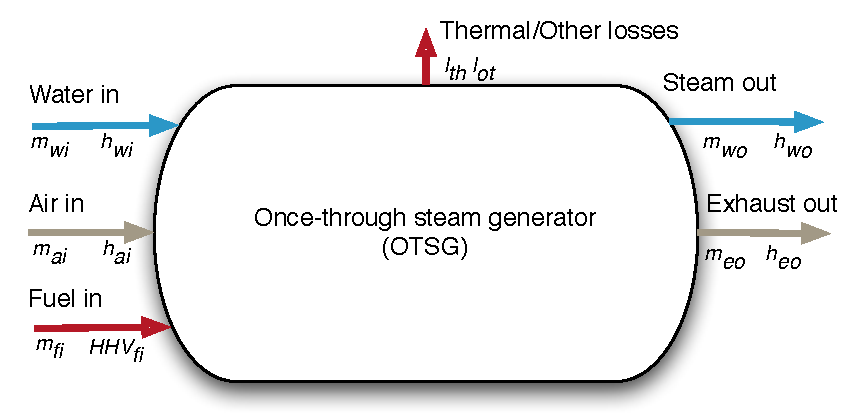
\includegraphics[width=0.65\columnwidth]{images/OTSG.pdf}
\caption{Once-through steam generator with mass and energy balance terms. Lower case terms are defined per lbmol of input fuel.}
\label{fig:OTSG}
\end{figure}

The operating conditions of combustion must be specified. These include the inlet air temperature $T_{a,in}$ [$^\circ$F], the outlet exhaust temperature $T_{e,out}$ [$^\circ$F] and the excess air in combustion $R_{a,comb}$ [mol O$_2$/ mol stoichiometric O$_2$].


\paragraph{Gaseous fuel combustion for steam generation}

The gas species tracked in the OTSG are described below in Section \ref{sec:properties_fuels}. \marginnote{Steam Generation 2.2.3} For an arbitrary fuel makeup, the composition, average molar mass, and lower heating value (LHV) are calculated.

OTSG inlet air composition, combustion stoichiometry, and excess air ratio are used to compute the mass of air required per lbmol of fuel consumed. For each reactive species, the reactants needed per mol of input fuel are computed: \marginnote{Fuel \\ Specs \\ Table 2.3}
%%%%%%%%%%%%%%
\begin{equation}\label{eq:steam_N_stoich_comb}
N_i = \frac{x_{a,i}}{x_{a,O2}}\left({x_{f,C} +\frac{x_{f,H}}{4}}\right) \quad\quad \footnotesize{\left[\frac{\text{lbmol}}{\text{lbmol fuel}}\right]}
\end{equation}
%%%%%%%%%%%%%%
where $N_i$ = number of moles of air species $i$ [mol]; $x_a,i$ = mole fraction of species $i$ in air [mol/mol]; $x_{f,C}$ = mol of carbon per mol of fuel (e.g., 2 for C$_2$H$_6$) [mol/mol]; and $x_{f,H}$ = mol of hydrogen per mol of fuel [mol/mol]. The sum over all species $i$ gives air required for stoichiometric combustion, which is multiplied by the excess air ratio $R_{a,comb}$ to get real air requirements:
\marginnote{Steam Generation 2.2.3}
%%%%%%%%%%%%%%
\begin{equation}\label{eq:steam_N_real_comb}
N_{a} = R_{a,comb}\sum_{i=1}^{n} N_i \quad\quad \footnotesize{\left[\frac{\text{lbmol air}}{\text{lbmol fuel}}\right]} 
\end{equation}
%%%%%%%%%%%%%%
Where $R_{a,comb}$ = ratio of combustion air to stoichiometric air [lbmol air / min lbmol air for combustion]. In this case there are $n$ species present in air.

At constant pressure the change in enthalpy with temperature is given as:
%%%%%%%%%%%%%%
\begin{equation}\label{eq:steam_dh}
\delta h = C_p \delta T \quad\quad \footnotesize{\left[\frac{\text{Btu}}{\text{lbmol}}\right]}
\end{equation}
%%%%%%%%%%%%%%
Specific heat capacity $C_p$ as a function of $T$ can be defined for gas species $i$ as \cite[Table A-2E]{Cengel2006}:
%%%%%%%%%%%%%%
\begin{equation}\label{eq:steam_cp}
C_{p,i}= a_i+b_iT + c_iT^2 + d_iT^3 \quad\quad \footnotesize{\left[\frac{\text{Btu}}{\text{bmol-$^\circ$R}}\right]} 
\end{equation}
%%%%%%%%%%%%%%
Which can be integrated between outlet and inlet temperatures
%%%%%%%%%%%%%%
\begin{equation}\label{eq:steam_hx}
h_i = \int_{T_{ref}=300}^{T} C_{p,i} dT = a_iT+\frac{b_i}{2}T^2 + \frac{c_i}{3}T^3 + \frac{d_i}{4}T^4 + e_i \quad \footnotesize{\left[\frac{\text{Btu}}{\text{lbmol}}\right]} 
\end{equation}
%%%%%%%%%%%%%%
where $e_i$ is a constant of integration. OPGEE sets $h$ = 0 at $T_{ref}$ = 300 K to solve for $e_i$. Terms $a$ through $d$ are given in OPGEE for N$_2$, O$_2$, CO$_2$, SO$_2$, air, H$_2$O$_{(v)}$ and fuel inputs (approximated as CH$_4$) \cite{Cengel2006}. \marginnote{Steam Generation 2.2.4}

For example, inlet air enthalpy is computed using the inlet air temperature:
\marginnote{Input Data \\ Table 4.1 - 4.6}
%%%%%%%%%%%%%%
\begin{equation}\label{eq:steam_h_gas}
h_{a,in} = \sum_{i=1}^{n}\left( a_i T_{a,in} +\frac{b_i}{2}T_{a,in}^2 + \frac{c_i}{3}T_{a,in}^3 + \frac{d_i}{4}T_{a,in}^4 + e_i \right) \quad\quad \footnotesize{\left[\frac{\text{Btu}}{\text{lbmol air}}\right]} 
\end{equation}
%%%%%%%%%%%%%%
where again we have $i \in 1 \ldots n$ components in air.

The outlet lbmol of \marginnote{Steam Generation 2.2.3} all gases per lbmol of fuel consumed are computed assuming complete combustion (e.g., no unburned hydrocarbons, no CO produced), and no reactions with nitrogen. 

The enthalpy of OTSG outlet exhaust $h_{e,out}$ is computed with eq.\ \marginnote{Steam Generation 2.5.1.4} \eqref{eq:steam_h_gas}, using user input OTSG exhaust outlet temperature $T_{e,out}$. In practice, efficient steam generation is achieved by reducing $T_{e,out}$ to as low as practicable, thus removing as much heat as possible from OTSG combustion products. $T_{e,out}$ has a lower limit due to the need to avoid condensing corrosive flue gas moisture onto heat transfer tubes \cite{Ganapathy2003}. 

A wide range of exhaust gas temperatures is cited. Buchanan et al. cite ideal (minimum) exhaust gas temperatures of 266 $^\circ$F [130 $^\circ$C] or higher \cite[p. 78]{Buchanan2009}. Other sources cite temperatures of 350 $^\circ$F \cite[p. 36]{Donaldson1989}, 400 $^\circ$F \cite[p. 227]{Chilingarian1987} and even greater than 550 $^\circ$F for older Russian units \cite[p. 181]{Baibakov1989} 

In some cases, the exhaust gas temperature is limited by the approach to the inlet water temperature. In SAGD operations hot produced water is used as inlet water, and $T_{e,out}$ comes to within 15 $^\circ$C of the inlet water temperature. An air preheater would allow utilization of this excess energy if hot produced fluids are used for water source \cite{Buchanan2009}.

In addition to \marginnote{Steam Generation 2.2.7.2} losses from flue gas exhaust, other losses occur in an OTSG. We lump all thermal losses into a thermal shell loss term. For simplicity, it is assumed that 4\% of fuel enthalpy is lost as thermal shell loss $\epsilon_{th}$ [Btu/lbmol fuel consumed]. Other losses (start up inefficiencies, fouling, etc.) $\epsilon_{ot}$ are assumed $\approx$1\% of the fuel LHV [Btu/lbmol fuel consumed]. These total losses are supported by references, which cite losses of approximately 4\% \cite{Ganapathy2003}.

The enthalpy available for transfer to the incoming water is given by the difference between incoming enthalpy sources (incoming combustion air, fuel inputs) and outgoing enthalpy sources (hot exhaust, shell losses, other losses):
%%%%%%%%%%%%%%
\marginnote{Steam Generation 2.6.3}
\begin{equation}\label{eq:steam_hcomb}
\Delta h_{comb} = LHV+ h_{a,in} - h_{e,out} - \epsilon_{th} - \epsilon_{ot} \quad\quad \footnotesize{\left[\frac{\text{Btu to water}}{\text{lbmol fuel}}\right]}
\end{equation}
%%%%%%%%%%%%%%
The efficiency of steam generation $\eta_{OTSG}$ (LHV basis) can be computed by comparing the enthalpy imparted on steam to the higher heating value of the fuel inputs:
%%%%%%%%%%%%%%
\marginnote{Steam Generation 2.2.7.4}
\begin{equation}\label{eq:steam_OTSG_eff}
\eta_{OTSG} = \frac{\Delta h_{comb}}{LHV} \quad\quad \footnotesize{\left[\frac{\text{Btu to steam}}{\text{Btu fuel}}\right]}
\end{equation}
%%%%%%%%%%%%%%

Using the enthalpy provided to steam and $\Delta h_{comb}$, the total fuel consumption rate required per day can be computed.
%%%%%%%%%%%%%%
\marginnote{Steam Generation 2.2.8.1}
\begin{equation}\label{eq:steam_mfuel}
m_{f} = \frac{Q_{ws} \Delta h_{ws}}{\Delta h_{comb}} \quad\quad \footnotesize{\left[\frac{\text{lbmol fuel}}{\text{d}}\right]}
\end{equation}
%%%%%%%%%%%%%%

\paragraph{Liquid fuels for steam generation}
Liquid fuels can be used for steam generation. In general, these are produced heavy crude oils that are consumed on site for steam generation. This was common practice in California TEOR developments until the 1980s, when air quality impacts stopped the practice.

Because liquid fuels do not have consistent molar compositions, computations generate lbm of fuel consumed. The heating value of crude oil as a function of \marginnote{Fuel Specs \\Table 1.1} API gravity is tabulated \cite{Schmidt1985}. The bulk chemical composition of crude oil is calculated \cite[p. 41]{Schmidt1985}. The mass fraction hydrogen $w_H$ as a function of crude specific gravity $sg$ is given as:
%%%%%%%%%%%%%%
\marginnote{Fuel Specs \\ Table 1.2}
\begin{equation}\label{eq:steam_wh}
w_H = a_H - 15 \gamma_o \quad\quad \footnotesize{\left[ \text{mass frac. H}\right]}
\end{equation}
%%%%%%%%%%%%%%
Where $a_H$ is a constant that varies with crude API gravity (and therefore specific gravity) as show in Table \ref{tab:hydrogen_const}.

\begin{table}
\caption{Hydrogen constant $a_H$ as a function of API gravity.}
\label{tab:hydrogen_const}
\begin{scriptsize}
\begin{tabular*}{0.5\columnwidth}{p{0.25\columnwidth}p{0.2\columnwidth}}
\toprule
API gravity & $a_H$ \\
\midrule
0 - 9 & 24.50\\
10 - 20 & 25.00\\
21 - 30 & 25.20 \\
31 - 45 & 25.45 \\
\bottomrule
\end{tabular*}
\end{scriptsize}
\end{table}


The mass fraction of \marginnote{Fuel Specs \\ Table 1.2} sulfur and other contaminants decreases with increasing API gravity, as seen in Figure \ref{fig:crude_contaminants} \cite[Ch. 8, tables 3, 4]{speight1994} \cite[Ch. 7, tables 2, 3, and 19]{speight1994} \cite{swafford2009}. We therefore include default values of $w_S$ that vary with API gravity from 5 wt.\% (API gravity 4-5) to 0.5 wt.\% (API gravity greater than 35). Nitrogen and oxygen content $w_N + w_O$ is assumed constant at 0.2 wt.\% and in element balance it is assumed to be entirely made up of N. Mass fraction carbon $w_C$ is calculated by difference using above mass fractions. Using the relative molar proportions of C, H, S, and N, the stoichiometric oxygen demand per carbon atom is computed assuming complete combustion. 

Using the oxygen requirement for combustion and the excess air ratio \marginnote{Steam Generation 2.2.3}$R_{a,comb}$, the lbmol of air required is computed similarly to eq.\ \eqref{eq:steam_N_real_comb} above. The inlet air enthalpy for combustion is computed using eq.\ \eqref{eq:steam_h_gas} above. The outlet exhaust composition is computed via element balance assuming complete oxidation (including S to SO$_2$). The outlet exhaust enthalpy is computed as in eq.\ \eqref{eq:steam_h_gas} for gaseous fuels combustion. The energy balance for combustion of liquid fuels is computed as in eq.\ \eqref{eq:steam_hcomb}.

\begin{figure}[t]
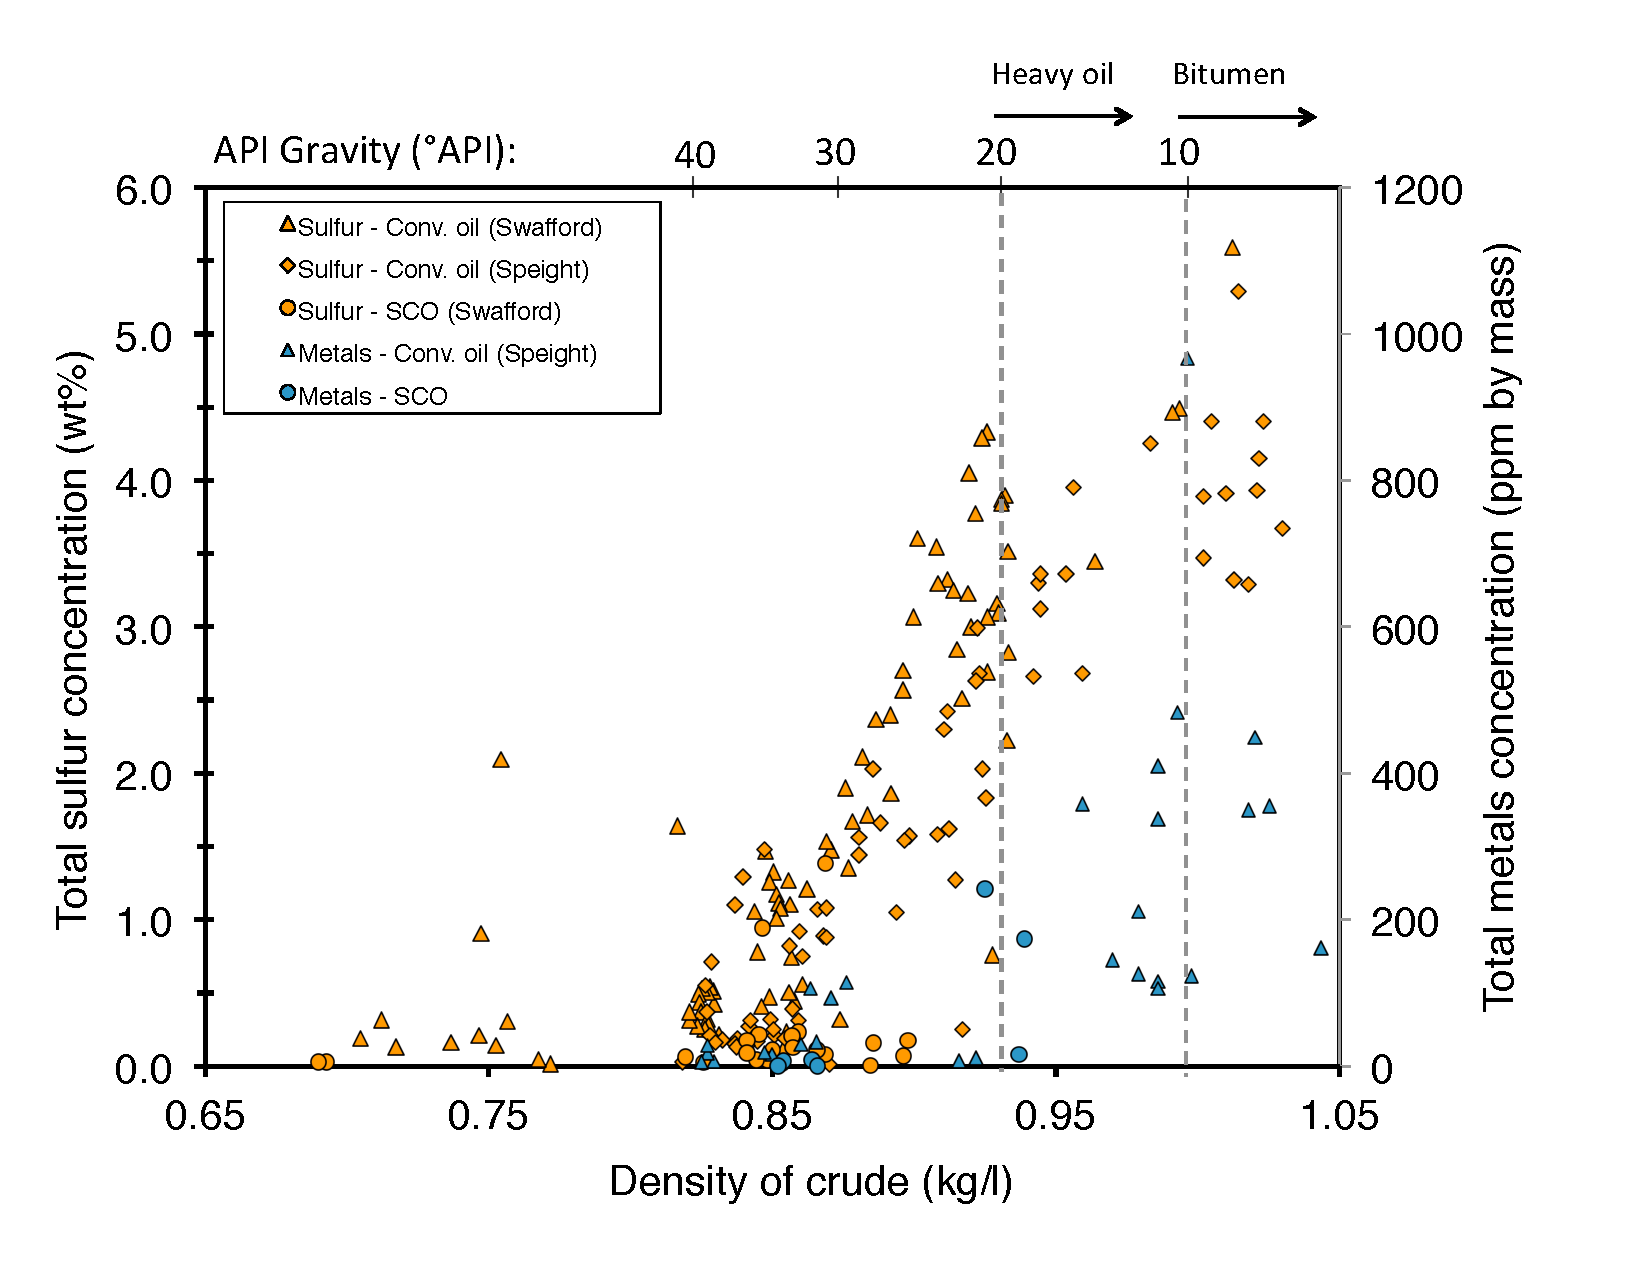
\includegraphics[width=0.8\columnwidth]{images/crude_contaminants.pdf}
\caption{Increase of crude contaminant load with increase in crude specific gravity (decrease in API gravity). Data from: Speight (1994) and Swafford (2009).}
\label{fig:crude_contaminants}
\end{figure}

\paragraph{Forced air blower in OTSG}

Combustion air is forced through the OTSG unit with a blower.\marginnote{Steam Generation 2.2.8.3} The power rating of the default OTSG blower is taken from COSIA documents outlining energy consumption and mass balances of a moderate-sized Steam-Assisted Gravity Drainage (SAGD) facility.  The COSIA OTSG has a combustion duty rating of 1488 mmBtu/h and an air blower power consumption rate of 3.7 MW.  This results in a consumption intensity of 0.139 bhp per mmBtu/d of OTSG consumption capacity.

\paragraph{High and medium pressure boiler feedwater pump}

The OTSG boiler must generate steam at pressures high enough to overcome frictional loss in the surface and subsurface piping as well as to allow flow into the reservoir.  The required pressure is supplied to the recycled produced water and makeup water depending on the mass fraction of each water stream.  This pressure is assumed supplied by an electrically-driven pump of large capacity.  For fields with low producing pressure, this consumption term is small.


\subsubsection{Gas turbine with heat recovery steam generator}

Cogeneration is used to co-produce electricity and steam for thermal oil recovery. \marginnote{Steam Generation 2.3} These systems combine a gas turbine (GT) with a heat recovery steam generator (HRSG) to produce steam from the exhaust gas of the gas turbine (see Figure \ref{fig:GT-HRSG}).  OPGEE allows the usage of supplemental gas firing in the post-turbine exhaust stream, sometimes called ``duct firing'', to allow for increased steam generation per unit of power output.

\begin{figure}[t]
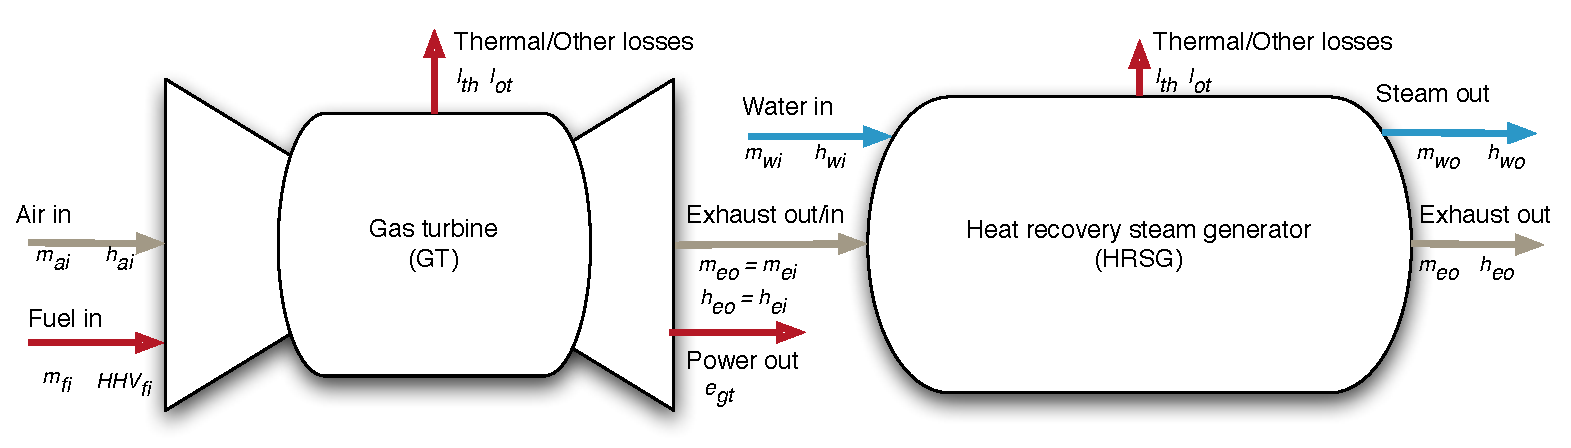
\includegraphics[width=1\columnwidth]{images/GT+HRSG.pdf}
\caption{Gas turbine plus heat recovery steam generator model. Mass flows represented by $m$ and energy flows represented by fuel lower heating value ($LHV$), electric power out ($e$) and enthalpy of gases ($h$).}
\label{fig:GT-HRSG}
\end{figure}

\paragraph{Gas turbine modeling} 

The chemical kinetics software tool Cantera \cite{Cantera2012} is used with MATLAB to compute the efficiency, losses, and turbine exit temperature for four hypothetical gas turbines labeled A, B, C, and D. The general method is as follows:
\begin{itemize}
\item Fuel and air compositions are specified in OPGEE for purchased natural gas (95\% CH$_4$, 3\% C$_2$H$_6$, 1.5\% C$_3$H$_8$, and 0.5\% inert) and air (dry air with 2\% moisture). 
\item The LHV of the fuel is computed assuming complete combustion.
\item Using the excess air fraction for a given turbine, the amount of O$_2$ (and therefore air) required relative to stoichiometric air requirements is used to compute relative air and fuel inputs into a mixture. The masses of fuel inputs $m_{f,in}$ and air inputs $m_{a,in}$ are normalized to a 1 kg mixture, as is default in Cantera.
\item The fuel and air mixture is equilibrated using the assumption of adiabatic combustion.
\item The enthalpy of products of adiabatic combustion is recorded as $h_{e}$, or the mass-specific exhaust enthalpy after combustion.
\item The enthalpy of products of combustion is computed when returned to initial conditions (300 K, 101.325 kPa) to compute the reference enthalpy $h_{e,atm}$.
\item The difference between the enthalpy of hot combustion products and the reference enthalpy of completely cool exhaust is partitioned into losses (pressure and temperature losses due to real machine imperfections), work provided by turbine ($W_{GT}$), and enthalpy of hot exhaust ($h_{e,out}$).
\item The resulting temperature of hot exhaust gases is computed.
\end{itemize}

The gas turbine model was tested against reported gas turbine data. Data for turbine heat rate, power output, turbine exhaust mass flow rate, and turbine exhaust temperature were collected for commercial turbines from Siemens, GE, and Hitachi \cite{Siemens2012, Badeer2012, Farmer2010}. The code assumes consistent 4\% thermal and other losses ($\epsilon_{th} + \epsilon_{ot}$) for each turbine. Results show excellent agreement between predicted turbine exhaust temperature and manufacturer-reported turbine exhaust temperatures (Figure \ref{fig:GT_predictions}).

\begin{figure}[t]
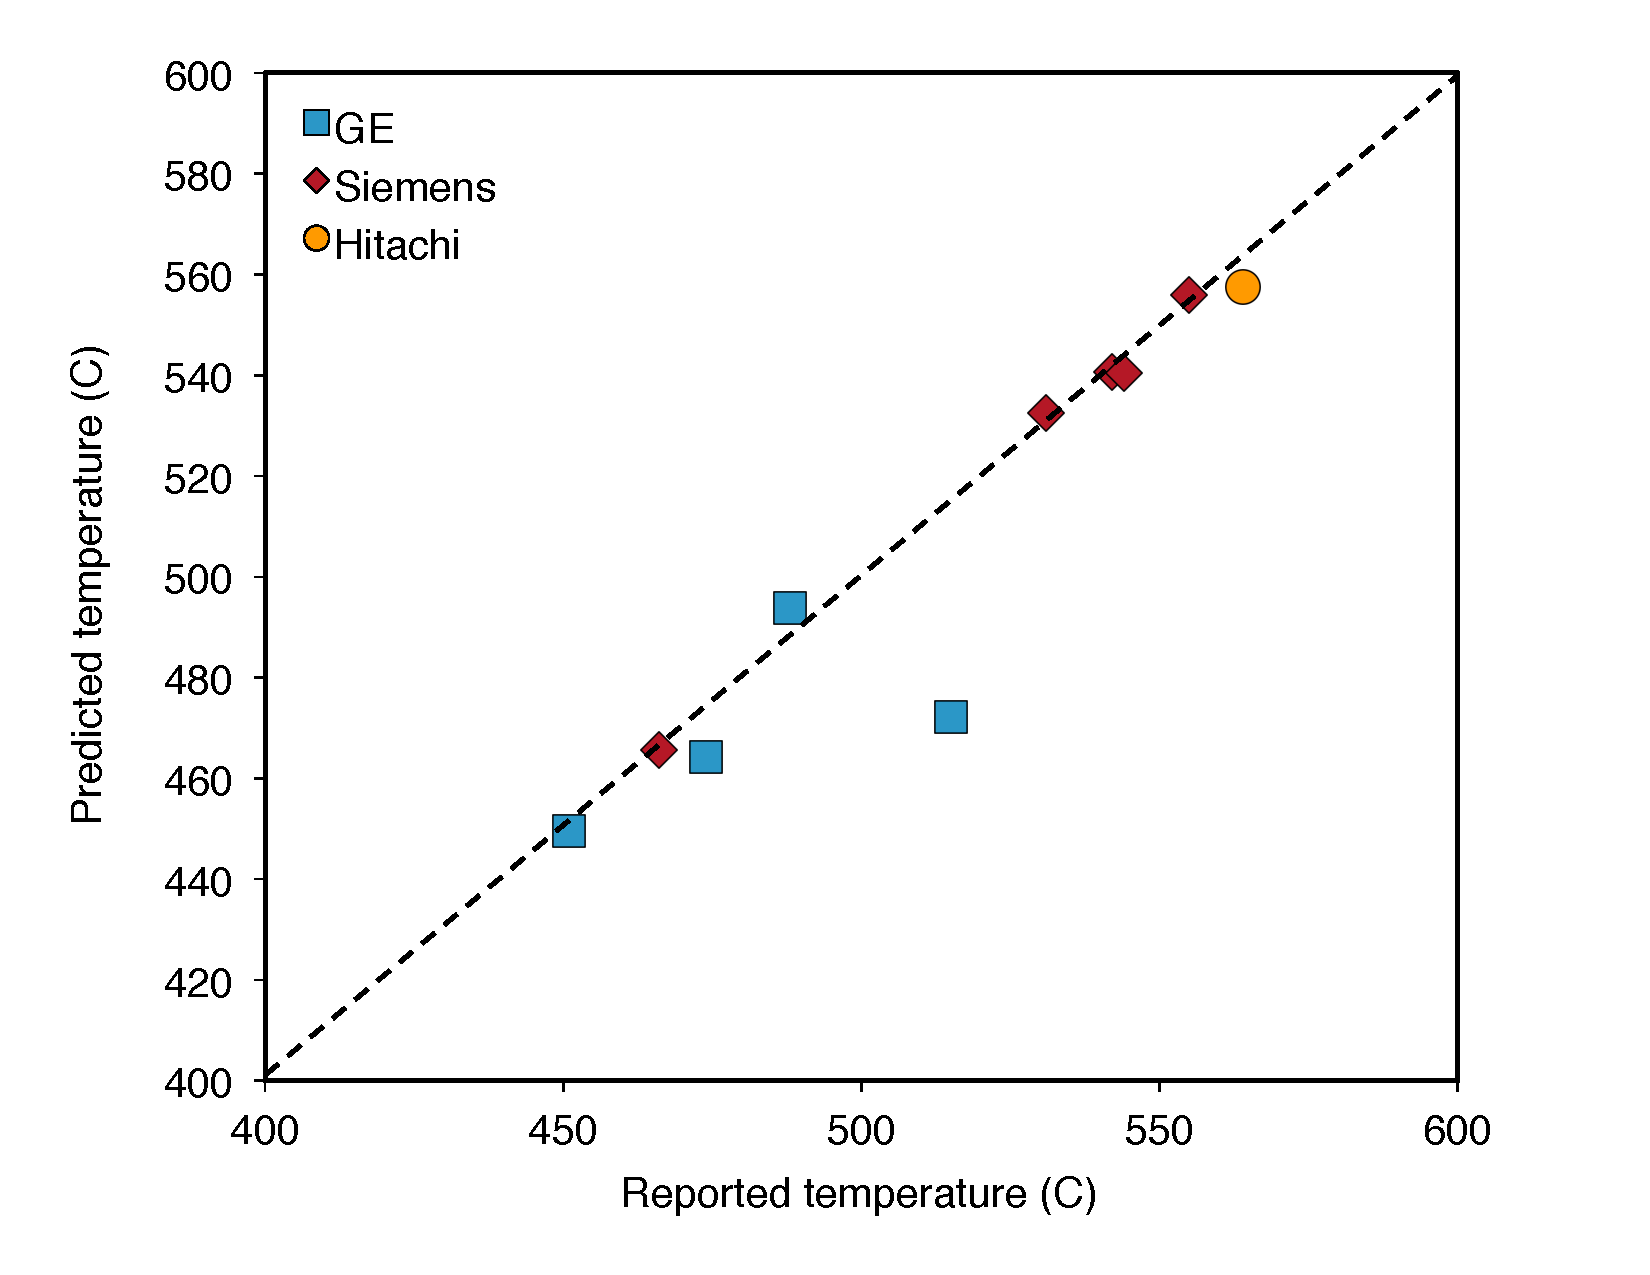
\includegraphics[width=0.8\columnwidth]{images/GT_predictions.pdf}
\caption{Predicted turbine exit temperatures for variety of turbines from literature (\emph{y-axis}) as compared to reported value from the literature (\emph{x-axis}). }
\label{fig:GT_predictions}
\end{figure}

The GT model is used to model four hypothetical turbines A - D, using characteristics similar to those specified by Kim \cite{Kim2004}. \marginnote{Input data \\ Table 3.1} The results from our code are used to generate required inputs for turbines A-D including turbine exhaust temperature [F], turbine efficiency [Btu e- per Btu LHV fuel input], turbine specific power [Btu e-/lb exhaust], turbine excess air [lbmol O$_2$ / lbmol stoichiometric O$_2$], and turbine loss factor [Btu/Btu LHV fuel input]. These results are shown in Table \ref{tab:GT_inputs}.

Using turbine efficiency and turbine loss from Table \ref{tab:GT_inputs}, \marginnote{Steam Generation 2.3.1} energy balances for each turbine are computed. Using turbine excess air ratios from Table \ref{tab:GT_inputs}, total air requirements per lbmol of fuel input to gas turbine are computed. \marginnote{Steam Generation 2.3.5} Inlet air enthalpy is computed as shown in eq.\ \eqref{eq:steam_h_gas}. Moles of combustion products are computed via stoichiometric relationships. \marginnote{Steam Generation 3.3.5.1} Using turbine exhaust temperature, turbine exhaust composition, and relationships from eq.\ \eqref{eq:steam_h_gas}, the enthalpy of gas turbine exhaust is computed.

The enthalpy of the gas turbine exhaust is the useful energy input to the HRSG. \marginnote{Steam Generation 2.3.5} Steam production via the HRSG is modeled analogously to that of the OTSG.


\begin{table}
\caption{Gas turbine model results for hypothetical turbines A-D. These results serve as input data to OPGEE GT model.}
\label{tab:GT_inputs}
\begin{scriptsize}
\begin{tabularx}{1\columnwidth}{p{0.3\columnwidth}p{0.2\columnwidth}p{0.08\columnwidth}p{0.08\columnwidth}p{0.08\columnwidth}p{0.08\columnwidth}}
\toprule
Parameter & Unit & Turb. A & Turb. B & Turb. C & Turb. D \\
\midrule
Turbine exhaust temp. &[$^\circ$F] & 932.0 & 947.9 & 950.0 & 1074.1\\
Turbine efficiency &$\left[\frac{\textrm{Btu e-}}{\textrm{Btu LHV}}\right]$ & 0.205 & 0.237 & 0.280 & 0.324\\ 
Turbine specific power & $\left[\frac{\textrm{Btu e-}}{\textrm{lb exhaust}}\right]$& 69.5 & 85.4 & 108.0 & 155.7\\ 
Turbine excess air & $\left[\frac{\textrm{Mol O$_2$ real}}{\textrm{Mol O$_2$ stoich.}}\right]$& 4.00 & 3.75 & 3.50 & 2.80\\
Turbine loss & $\left[\frac{\textrm{Btu loss}}{\textrm{Btu LHV}}\right]$& 0.041 & 0.036 & 0.032 & 0.027\\ 
\bottomrule
\end{tabularx}
\end{scriptsize}
\end{table}

\paragraph{Forced air blower in HRSG}

It is assumed that no forced air blower is required in an HRSG due to the high exit velocities of turbine exhaust.

\paragraph{Duct firing}

Duct firing increases the amount of steam generated from the gas turbine exhaust stream by heating the exhaust stream through supplemental combustion in the inlet of the HRSG. Because GTs operate with large amounts of excess air (air input = 2-3 times stoichiometric requirement), large amounts of residual oxygen remain the GT exhaust.

Duct firing is turned on at the top of the steam generation sheet.\marginnote{Steam Generation 1.2.7.2.3}.  If duct firing is selected, the GT exhaust temperature remains as selected from input data, but the effective HRSG inlet temperature is assumed to increase to 1300 $^\circ$F \cite[Table 5, Case 2]{Ganapathy1996}.  The computed additional fuel required to duct fire to the desired temperature is computed using the composition of HRSG inlet gas to compute the effective heat capacity of the gas, which gives an approximate additional fuel needed to raise temperature (thus avoiding an iterative calculation). \marginnote{Steam Generation 2.3.8.4} If very different conditions are selected (e.g., turbine or post-duct firing temperature), this approximate fuel consumption factor should be adjusted by the user.

Duct firing increases the efficiency of the HRSG, but this efficiency gain is somewhat offset by the loss of exported electricity per unit of steam generated. This reduces the co-production credit received by the cogeneration system and negates some of the potential GHG intensity reductions associated with duct firing.


\subsubsection{Solar thermal steam generation}

\marginnote{Steam Generation 2.4}  Solar thermal steam generation is modeled to allow for partial displacement of natural gas in steam generation thermal needs.  The fraction of steam generated using solar thermal is provided by the user on the \sheet{Inputs} sheet. \marginnote{Inputs 1.4.13}  That fraction of steam is then provided by the solar thermal system at no cost of natural gas. Solar thermal pumping work for solar HTF circulation is calculated assuming that HTF pumping scales similarly to air blower work for OTSG steam generation (personal communication, John O'Donnell GlassPoint energy).\marginnote{Steam Generation 2.4.2.2}

Reasonable fractions of energy displaced by solar thermal are around 15-25\% in the absence of thermal storage or modification of steam injection schedule \cite{Wang2016, Sandler2014, Palmer2015}. If steam injection schedule is modified to only inject steam during daytime solar hours, then the fraction of steam generated with solar thermal can approach complete NG displacement.

\subsection{Defaults for steam injection}

\subsubsection{General default parameters}

Parameters and variables in the steam injection model are listed below in Table \ref{tab:defaults_steam}.


\subsubsection{Defaults for SAGD operations}

Default data for Canadian SAGD operations are taken from a variety of public sources.  The overall approached to collecting data inputs for OPGEE is use the COSIA template (Base case, warm lime softening- OTSG) \cite{COSIA2014} wherever possible to provide default input data to OPGEE to estimate emissions for SAGD operations \cite{COSIA2014}. When the template does provide the required data, we supplement that data with AER company reported data including statistical reports \cite{AERvar} and in situ performance presentations \cite{AERvarISPP} and expert feedback when no public data is available.

\paragraph{Production method}
SAGD and CSS projects use gas lift or mechanical lift (downhole pump) and steam flooding for oil production. In mechanical lift, electric submersible pump (ESP), progressive cavity pump (PCP) and rod pump are used. OPGEE calculations can be modified based on the characteristics of these pump types.
In the COSIA SAGD reference facility, mechanical lift via ESP, with downhole pressure of 2.2 MPa, is used \cite{COSIA2014}.

\paragraph{Gas handling properties: GOR, flaring, and venting}
These gas volume parameters are reported as a dimensionless value in AER statistical reports \cite{AERvar}. We assume that the value is in m$^3$ gas per m$^3$ bitumen, and convert to the desired unit (scf/bbl bitumen). The resulting values for all three gas volumes are much lower than conventional defaults, which is expected due to small quantities of associated gas in bitumen deposits.

\paragraph{Field properties: productivity index, pressure, depth}
The difference between reservoir pressure and the injection downhole pressure is reported around 350 kPa for the Firebag project \cite{AERvarISPP}. Using this value and other Firebag project data, productivity index (PI) is calculated around 22 bbl/(psi-d). This default is reasonable for SAGD projects in general due to the fact that at SAGD conditions, even large changes in PI do not affect the results significantly.   The default high pressure steam system operates at 1400 psia \cite{COSIA2014}.  Field depth of in situ extraction in current SAGD operations is 1300-2000 ft \cite{COSIA2014}.

\paragraph{Steam generation technology}
Default steam generation technology from the COSIA template is a once-through-steam generator fired with (primarily) purchased gas.  The OTSG requires forced air blowers and boiler feedwater pumps to increase pressure of both produced water and makeup water.  The water is treated before boiling in a warm lime softener/evaporator.








\begin{landscape}
\begin{scriptsize}
\tablefirsthead{\toprule Param. & Description & Eq. no. & Default & Lit. range & Unit & Sources & Notes\\
\midrule}
\tablehead{ \multicolumn{8}{p{1\columnwidth}}{\textit{Continued from previous page}}\\ \toprule Param. &Description & Eq. no. &Default & Lit. range & Unit & Sources & Notes \\ 
\midrule }
\tabletail{\bottomrule \multicolumn{8}{p{1\columnwidth}}{\textit{Continued on next page...}}\\}
\tablelasttail{\bottomrule}
\tablecaption{Default inputs for steam injection calculations.}
\label{tab:defaults_steam}
\begin{supertabular*}{1\columnwidth}{p{0.05\columnwidth}p{0.3\columnwidth}p{0.05\columnwidth}p{0.05\columnwidth}p{0.1\columnwidth}p{0.17\columnwidth}p{0.1\columnwidth}p{0.04\columnwidth}}
$a_H$ & Crude hydrogen fraction constant & - & Table \ref{tab:hydrogen_const} & - & [lbm H / lbm crude oil] & \cite{Schmidt1985} & \\
$a_i \ldots e_i $ & Species-specific heat capacity constants & - & var. & - & [various] & \cite{Cengel2006} &\\
$C_{p} $ & Heat capacity at constant pressure & \eqref{eq:steam_cp} & - & - & [Btu/lbmol-$^\circ$R] & &\\
$\eta_{OTSG}$ & OTSG efficiency & \eqref{eq:steam_OTSG_eff} & - & - & [Btu steam / Btu LHV fuel] & & \\
$\epsilon_{th}$ & Thermal losses from OTSG & - & 0.04 & - & [Btu/Btul fuel] & \cite{Ganapathy2003} & \\
$\epsilon_{ot,ng}$ & Other losses from OTSG fueled with natural gas & - & 5000 & - & [Btu/lbmol fuel] & \cite{Ganapathy2003} & c \\
$\epsilon_{ot,co}$ & Other losses from OTSG fueled with crude oil & - & 250 & - & [Btu/lbml fuel] & \cite{Ganapathy2003} & c \\
$\epsilon_{ws}$ & Steam pressure loss factor & - & 1.25 & 0.1 - 0.5 & [frac.] & \cite{Chilingarian1987} & d \\
$\lambda_{ng}$ & Fraction natural gas & - & 1 & 0 - 1 & [frac] & - & b \\
$\lambda_{pg}$ & Fraction processed associated gas & - & 0 & 0 - 1 & [frac] & - & b \\
$h_{a,in} $ & Inlet air enthalpy & \eqref{eq:steam_h_gas} & - & - & [Btu/lbmol] & & \\
$h_{e,out} $ & Enthalpy of OTSG exhaust & \eqref{eq:steam_h_gas} & - & - & [Btu/lbmol] & & \\
$h_{ws,f}$ & Enthalpy of liquid phase water in steam & - & var. & 180 - 730 & [Btu/lbm] & & \\
$h_{ws,g}$ & Enthalpy of vapor phase water in steam & - & var. & 1090 - 1205 & [Btu/lbm] & & \\
$h_{ws}$ & Enthalpy of injected steam ($<$ 100\% quality) & \eqref{eq:steam_hs} & - & - & [Btu/lbm] & &\\
$h_{w,in}$ & Inlet water enthalpy & - & 9.8 & - & [Btu/lbm] & &\\
$\Delta h_{ws}$ & Change in water enthalpy upon boiling & \eqref{eq:steam_hw} & - & - & [Btu/lbm] & &\\
$\Delta h_{comb} $ & Heat available from combustion to water & \eqref{eq:steam_hcomb} & - & - & [Btu / lbmol fuel] & &\\
$h_i $ & Enthalpy of species $i$ & \eqref{eq:steam_hx} & - & - & [Btu/lbmol] & & \\
$LHV$ & Lower heating value of fuel & - & var. & - & [Btu LHV / lbmol fuel] & & \\
$N_i$ & Number of moles of air species $i$ & \eqref{eq:steam_N_stoich_comb}& - & - & [lbmol] & & \\
$N_{a}$ & Number of moles of air for real (non-stoichiometric) combustion & \eqref{eq:steam_N_real_comb} & - & - & [lbmol] & &\\
$p_{w,in}$ & Inlet water pressure & - & = $p_s$ & - & [psia] & &\\
$p_{ws}$ & Steam pressure & \eqref{eq:steam_ps} & - & - & [psia] & &\\
$Q_o$ & Quantity of oil produced & - &1000 & - & [bbl oil/d] & & \\
$Q_{ws}$ & Steam required & \eqref{eq:steam_qs} & - & - & [lbm water/d] & - & \\
$R_{a,comb} $ & Excess air combustion ratio & - & 1.2 & 1.075 - 1.25 & [lbmol air/lbmol air stoich.] & & e \\
$\rho_{w}$ & Density of water & - & 350.4 & - & [lbm/ft$^3$] & \cite{EngToolbox} & f \\
$\gamma_o$ &Crude specific gravity &\eqref{eq:production_API_gravity}& - & - & [-] & & \\
$SOR$ & Ratio of steam injected to oil produced & - & 3.0 & 2.5 - 6 & [bbl water/bbl oil] & \cite{DOGGR2011, ERCB2011a} &g \\ 
$T_{a,in} $ & Inlet air temperature & - & 540 & 500 - 560 & [$^\circ$R] & & h \\
$T_{e,out}$ & Temperature of OTSG exhaust & - & 810 & 725 - 910 & [$^\circ$R] & [various] & i \\
$T_{w,in}$ & Inlet water temperature & - & 40 & - & [$^\circ$F] & & j \\
$T_{ws}$ & Steam temperature & - & var. & - & [$^\circ$F] & & \\
$w_H$ & Mass fraction hydrogen in crude & \eqref{eq:steam_wh} & - & - & [lbm H / lbm oil] & & \\
$x_{a,i}$ & Mole fraction of species $i$ in air & - & var. & - & [lbmol/lbmol] & & m \\
$x_C$ & Moles of carbon per mole of fuel & - & var. & - & [lbmol/lbmol] & & a \\
$x_H$ & Moles of hydrogen per mole of fuel & - & var. & - & [lbmol/lbmol] & & a \\
$X_s$ & Steam quality & - & 0.8 & - & [lbm vap./lbm steam] & \cite{Green1998} & k \\
$y_{ng}$ & Binary variable: gaseous fuel in OTSG& - & 1 & 0 or 1 & [y/n] & - & l \\
$y_{co}$ & Binary variable: crude oil in OTSG & - & 0 & 0 or 1 & [y/n] & - & l \\
\midrule
\multicolumn{8}{p{1\columnwidth}}{\emph{a} - See \sheet{Fuel specs} Table 2.3 for combustion factors for gas inputs.}\\
\multicolumn{8}{p{1\columnwidth}}{\emph{b} - Assumption: Gas is purchased due to typical low GORs for heavy crudes.}\\
\multicolumn{8}{p{1\columnwidth}}{\emph{c} - Assumption to account for incomplete combustion, fouling, warm up and cool-down, and other real-world inefficiencies.} \\
\multicolumn{8}{p{1\columnwidth}}{\emph{d} - Piping friction losses can represent 10-50\% of the steam pressure developed at the outlet of the steam generator." \cite[p. 228]{Chilingarian1987}} \\
\multicolumn{8}{p{1\columnwidth}}{\emph{e} - Conservative assumption for input excess air. Can be lower with special combustion equipment. } \\
\multicolumn{8}{p{1\columnwidth}}{\emph{f} - Fresh water input} \\
\multicolumn{8}{p{1\columnwidth}}{\emph{g} - Common SOR for efficient TEOR project. Range is quite variable, especially in early years of steam injection.} \\
\multicolumn{8}{p{1\columnwidth}}{\emph{h} - Equal to 300 K. Chosen for ease of gas turbine modeling. } \\
\multicolumn{8}{p{1\columnwidth}}{\emph{i} - Equal to 350 $^\circ$F. Reported range is wide in literature. See \cite{Buchanan2009, Donaldson1989, Chilingarian1987, Baibakov1989}.} \\
\multicolumn{8}{p{1\columnwidth}}{\emph{j} - Assumption for cool water inlet. }\\
\multicolumn{8}{p{1\columnwidth}}{\emph{k} - Most commonly cited steam quality. Other qualities cited include 75\%.} \\
\multicolumn{8}{p{1\columnwidth}}{\emph{l} - Assumption: Most steam generation in California and Alberta is natural gas fired.}\\
\multicolumn{8}{p{1\columnwidth}}{\emph{m} - See \sheet{Input Data} Table 2.4 for air composition.}\\
\end{supertabular*}
\end{scriptsize}
\end{landscape}



\clearpage



%%%%%%%%%%%%%%%%%%%%%%%%%%%%%%%%%%%%%
\section{Flaring}
\label{sec:flaring}



Flaring is used to dispose of associated natural gas produced during bulk separation (see Section \ref{sec:surface_processing}) when it cannot be used economically. Gas flaring resulted in emissions of 0.28 Gt CO$_2$ eq.\ in 2008, or about 1\% of global GHG emissions \cite{Elvidge2009}.  Since 1994, NOAA National Geophysical Data Center has estimated flaring volume using satellite imagery \cite{Elvidge2009}. The distribution of estimate flaring volume by country is highly skewed; in 2008 Russia, Nigeria, Iran, and Iraq were the country with the highest flaring volumes \cite{Elvidge2009}.


The streams flowing into and out of the flaring process are shown in Figure \ref{fig:flaring_PF} and are listed in Table \ref{tab:flaring_PF}.


%%%%%%%%%%%
\begin{table}
\caption{Streams flowing into and out of the flaring process. I/O denotes input or output stream}
\label{tab:flaring_PF}
\begin{scriptsize}
\begin{tabularx}{1\columnwidth}{p{0.32\columnwidth}p{0.05\columnwidth}p{0.04\columnwidth}p{0.32\columnwidth}p{0.05\columnwidth}p{0.05\columnwidth}}
\toprule
Flow name							& Stream   			& I/O 	& Source/Destination       			& Units 			&  Notes\\ 
\midrule
Gas after separator						& \stream{28}			& I		& Separator					& [t/d]			&			\\
Mine offgas to flare						& \stream{84}			& I		& Mining						& [t/d]			&			\\
\midrule
Gas consumed in flare		 			& \stream{29}			& O		& Environment					& [t/d]			&			\\
Post-flare gas to vent					& \stream{30}			& O		& Venting						& [t/d]			&			\\
\bottomrule
\end{tabularx}
\end{scriptsize}
\end{table}
%%%%%%%%%%%


%%%%%%%%%%%
\begin{figure}
\includegraphics[width=0.85\columnwidth]{images/flaring_PF.pdf}
\caption{Streams flowing into and out of the flaring process. All streams measured in tonnes per day excepting electricity which is measured in MWh/d.}
\label{fig:flaring_PF}
\end{figure}
%%%%%%%%%%%



\subsection{Calculation of flaring emissions} \label{sec:flaring_emissions}


For the calculation of flaring emissions, the key input parameter is the flaring-to-oil ratio, or FOR [scf/bbl]. The FOR is converted into flaring volume using the volume of oil produced: \marginnote{Flaring \\ 1.3}
%%%%%%%%%%
\begin{equation} \label{eq:flaring_volume}
Q_{F}= \frac{FOR \cdot Q_{o}}{10^6} \quad \footnotesize{\text{[MMscf/d]}}
\end{equation}
%%%%%%%%%%
where $Q_{F}$ = flaring volume [MMscf/d]; $FOR$ = flaring-to-oil ratio [scf/bbl of oil]; and $Q_{o}$ = volume of oil produced [bbl/d].

The OPGEE default FOR is given by country-level flaring data \cite{NOAA2010} and production volumes \cite{EIA2010} for the years 2010 to 2015. \marginnote{Flaring \\ Table 4.1}  A detailed listing of sources and compilation notes for flaring data is given in Table \ref{tab:flaringdata}. The default flaring rate is retrieved from the \sheet{Flaring} worksheet based on the field location specified in the \sheet{Active Field} worksheet. The flaring rate in a specific oil field could be significantly higher or lower than the country-average. In the case no default is available for the specified field location, the world average is taken as the default value.

\begin{table}
\begin{scriptsize}
\caption{Sources of flaring data and construction notes}
\label{tab:flaringdata}
\begin{tabular*}{1\columnwidth}{p{0.03\columnwidth}p{0.45\columnwidth}p{0.45\columnwidth}}
\toprule
	 & Flaring volumes & Oil production volumes \\
\midrule
2010 & OPGEE 1.1e, \sheet{Flaring} worksheet & BP 2016 Statistical Review of World Energy. If unavailable, EIA International Petroleum Production, data series ``Total Petroleum and Other Liquids'' \\
2011 & OPGEE 1.1e, \sheet{Flaring} worksheet & \emph{ibid.} \\
2012 & Dataset obtained from Chris Elvidge via Jim Duffy, California Air Resources Board, July 21st, 2015. Contains country-level totals from NOAA analysis & \emph{ibid.} \\
2013 & World Bank Global Gas Flaring Reduction Partnership, website accessed 5/30/2017 & \emph{ibid.} \\
2014 & \emph{ibid.} &\emph{ibid.} \\
2015 & \emph{ibid.} &\emph{ibid.} \\
\bottomrule
\end{tabular*}
\end{scriptsize}
\end{table}

Carbon-dioxide-equivalent flaring emissions are calculated from the flaring volume using the flare efficiency $\eta_F$. \marginnote{Flaring \\ 3.1}The flare efficiency is the fraction of flared gas that is combusted. The remaining gas undergoes fuel stripping and is emitted as unburned hydrocarbons. 

Flare efficiency varies with flare exit velocities and diameters, cross wind speed, and gas composition \cite{Johnson2001, Johnson2008}. For example, flare efficiencies in Alberta were estimated to range from 55\% to $\geq 99$\%, with a median value of 95\%, adjusted for wind speed distributions \cite{Johnson2008}. 

If the user does not have field specific information about the flare system design and average ambient wind conditions,\marginnote{Flaring \\ 1.1} then OPGEE populates the model with a default flare efficiency of 95\%. If the user has the full amount of required data (see Table \ref{tab:flaring_data_reqs}) then the user can determine the field-specific flaring efficiency.

The logical progression of the flaring worksheet is shown as a flow-chart in Figure \ref{fig:flaring_logic}.

\begin{figure}[t]
\includegraphics[width=1\columnwidth]{images/flaring_logic.pdf}
\caption{Flowchart illustrating the logic of the flaring computation worksheet.}
\label{fig:flaring_logic}
\end{figure}

\begin{table}
\begin{scriptsize}
\caption{Data requirements for utilizing field-specific flaring calculation.}
\label{tab:flaring_data_reqs}
\begin{tabular*}{1\columnwidth}{p{0.4\columnwidth}p{0.3\columnwidth}}
\toprule
Data requirement & Units \\
\midrule
Oil production & [bbl/d]\\
Flaring intensity & [scf/bbl] \\
Number of flares & [\#]\\
Number of flare tips per flare & [\#]\\
Flare tip diameter & [in]\\
Lower heating value of gas (LHV) & [MJ/kg] or [Btu/scf]\\
Average wind speed & [mph]\\
\bottomrule
\end{tabular*}
\end{scriptsize}
\end{table}



OPGEE uses a flare efficiency equation developed by Johnson and Kostiuk \cite{Johnson2002}: \marginnote{Flaring 3.1}
\begin{equation}\label{eq:flare_eta}
\eta_F =1-\frac{A \,\textrm{exp}\left[{\frac{BU_{\infty}}{\left(gVd\right)^\frac{1}{3}}}\right]}{LHV^3}
\end{equation}
Where $A$ = 156.4 [MJ/kg], $B$ = 0.318 [dimensionless], $U_{\infty}$ is the wind velocity [m/s], $g$ is the gravitational constant [m/s$^2$], $V$ is flare gas exit velocity [m/s], $d$ is flare pipe exit diameter [m], and $LHV$ is the lower heating value of the flare gas [MJ/kg]. The most impactful parameters on flare efficiency are wind speed, gas exit velocity, and LHV. For completeness, all parameters are discussed below.

A second parametric model by Gogolek was explored \cite{Gogolek2012}, but for ease of integration into OPGEE, the Johnson model was selected.
\subsubsection{Constants}
The Johnson and Kostiuk model, contains different values for $A$ and $B$ given for methane flares and propane flares (the two flare gasses tested in the experiments). We implement the constants for methane flares for two reasons: first, the primary gas component in most flares is methane, and second, there is no simple direct linear relationship that can be used to interpolate the $A$ and $B$ values when non-pure gas mixtures are flared.
\subsubsection{Lower heating value}
The flare gas LHV is calculated by multiplying the LHV for each component of the gas by that component's mass fraction. \marginnote{Flaring \\ 1.4} The mass fraction of each gas species is taken from the \sheet{Gas Balance} worksheet, and the LHV for each species is taken from the \sheet{Fuel Specs} worksheet. If the flare gas has significant non-combustibles like N$_2$ and CO$_2$, the LHV of the gas, and thus the flare efficiency, will be reduced.
\subsubsection{Flare gas exit velocity and diameter}

There are cases where multiple wells feed to a single flare. There are also cases where each flare stack has multiple openings (flare tips) out of which gas exits. To calculate an efficiency, we are interested in the velocity of the gas coming out of each individual flare tip. As such, the user is asked to enter the number of wells per flare \marginnote{Flaring \\ 2.1.2} and the number of flare tips per flare. \marginnote{Flaring \\ 2.1.4} The volumetric flowrate of gas exiting through each opening is found by dividing the total flowrate for the field by the number of flare tips in the field.

Some flare tips have a variable orifice diameter, to allow for more even combustion properties under varying flow conditions. The user therefore first chooses whether they have a fixed diameter flare or a variable diameter flare.\marginnote{Flaring \\ 2.2.1} If the user chooses a variable tip diameter, then they choose a flow rate to size the flare to. Suggested maximum regulated flare exit velocity are given in the notes section of this entry. A US EPA regulatory standard is used. For onshore U.S. production, the EPA 60.18 40 CFR Ch.1 \cite{EPA2010} regulation states that for flares with a LHV of between 200 and 1,000 btu/scf, the maximum allowable gas exit velocity is 122 feet/sec. For flares with a LHV above 1,000 btu/scf, the maximum allowable gas exit velocity is 400 feet/sec \cite{EPA2010}. \marginnote{Flaring \\ 2.2.2.1} 

Users with pipe diameter information can enter that information. \marginnote{Flaring \\ 2.2.3.2} The flare pipe exit diameter is used directly in the Johnson and Kostiuk model, and is also used to calculate the flare gas exit velocity. Flare gas exit velocity is calculated by dividing the mass flux of gas by the cross sectional area of the pipe. \marginnote{Flaring \\ 2.2.3.3}

\subsubsection{Volume of gas flared}
If the user knows the volume of gas that is flared in their field, they can input these data. \marginnote{Flaring \\ 1.3} Otherwise, OPGEE estimates this number based on what country the user selected on the \sheet{Active Field} worksheet. \marginnote{Flaring \\ Table 4.1}

\subsubsection{Wind Speed}
The user must enter an average wind speed for their field. \marginnote{Flaring \\ 2.3} If the user is onshore in the United States, the user can select a local area from the dropdown list, and this will populate the wind speed cell with an average local wind speed. National Oceanic and Atmospheric Administration data on the average wind speed for hundreds of locations across the United States. \marginnote{Flaring \\ Table 4.2}

Because the efficiency of combustion \eqref{eq:flare_eta} has an exponential dependence on wind speed, a seemingly small increase in wind speed can significantly alter flare efficiency and thus emissions as well. As such, using a yearly average wind speed to calculate flaring efficiency can yield an inaccurate result. To resolve this, the Rayleigh probability distribution method has been adapted and applied from da Rossa \cite{daRosa2012}. Figure \ref{fig:wind_fits} illustrates the fit of the Rayleigh distribution to National Renewable Energy Laboratory wind data for 6 randomly chosen wind sites in the western United States.

\begin{figure}[tb]
\begin{center}
\subfigure[]{\label{fig:winda}\includegraphics[width=0.48\columnwidth]{images/wind1.pdf}}
\hfill
\subfigure[]{\label{fig:winda}\includegraphics[width=0.48\columnwidth]{images/wind2.pdf}}
\hfill
\subfigure[]{\label{fig:winda}\includegraphics[width=0.48\columnwidth]{images/wind3.pdf}}
\hfill
\subfigure[]{\label{fig:winda}\includegraphics[width=0.48\columnwidth]{images/wind4.pdf}} 
\hfill
\subfigure[]{\label{fig:winda}\includegraphics[width=0.48\columnwidth]{images/wind5.pdf}} 
\hfill
\subfigure[]{\label{fig:winda}\includegraphics[width=0.48\columnwidth]{images/wind6.pdf}}
\caption{Rayleigh distribution fit to 6 wind speed datasets from western United States. Data source: NREL Western Wind Integration Dataset.}
\label{fig:wind_fits}
\end{center}
\end{figure}

The Rayleigh method estimates a wind velocity probability distribution based on what is known about wind speeds. In this case, the user input average (mean) wind speed. This method estimates a mode (most frequently occurring wind speed) using the relationship: 
\begin{equation}
m_U = \frac{\mu_U}{\sqrt{\frac{\pi}{2}}}
\end{equation}
where $m_U$ is the mode of the windspeed [mph], and $\mu_U$ is the average (mean) windspeed [mph].

The probability density curve for the Rayleigh distribution is calculated from the mode using the expression: 
\begin{equation}
p(U) = \frac{U}{m_{U}} \textrm{exp}\left[-\frac{1}{2}\left(\frac{U^2}{m_U^2}\right)\right]
\end{equation}
where $p(U)$ is the probability of finding wind speeds of velocity $U$ [mph].

To calculate an overall flaring efficiency, the efficiency of combustion at each wind speed along the probability density curve is calculated using \eqref{eq:flare_eta}, and efficiencies are summed by their fractional probability. Figure \ref{fig:wind_example} shows the probability distribution for an average wind speed of 30 mph.
Using the Johnson and Kostiuk (2002) model with these data, OPGEE calculates the flaring combustion efficiency. \marginnote{Flaring \\ 3.1}

\begin{figure}[t]
\includegraphics[width=1\columnwidth]{images/wind30mph.pdf}
\caption{Example of OPGEE wind speed distribution for a 30 mph average windspeed input.}
\label{fig:wind_example}
\end{figure}


\subsection{Emissions from flares}

Emissions from non-combusted gas are calculated using the composition of associated gas from the \sheet{Gas Balance} worksheet: \marginnote{Flaring \\ 3.2.2.1}
%%%%%%%%%%
\begin{equation} \label{eq:flare_emissions_stripping}
EM_{F,str} = Q_{F}(1-\eta_{F}) \sum_i x_i \rho _{i} GWP_{i} \quad \quad \footnotesize{\text{[tCO$_{2}$eq/d]}}
\end{equation}
%%%%%%%%%%
where $EM_{F,str}$ = flaring emissions from stripped, non-combusted gas [tCO$_{2}$eq/d]; $\eta_{F}$ = flaring efficiency [\%]; $Q_{F}$ = flaring volume [MMscf/d]; $i$ = index of gas species CO$_{2}$, CH$_{4}$, and volatile organic compounds C$_{2}$H$_{6}$, C$_{3}$H$_{8}$ and C$_{4}$H$_{10}$; $x_i$ = molar fraction of gas component $i$ [mol/mol]; $\rho _{i}$ = density of gas component $i$ [g/ft$^{3}$]; and $GWP_{i}$ = GWP of gas component $i$ [g CO$_2$ eq.\ /g gas]. 

Emissions from flare combustion products assume complete combustion: \marginnote{Flaring \\ 3.2.1.1}
%%%%%%%%%%
\begin{equation} \label{eq:flare_emissions_combustion}
EM_{F,comb} = Q_{F} \eta_{F} \sum_i x_i \rho _{i} \Pi_{i} \quad \quad \footnotesize{\text{[tCO$_{2}$eq/d]}}
\end{equation}
%%%%%%%%%%
where $EM_{F,comb}$ = flaring emissions from combusted gas [tCO$_{2}$eq./d]; $\Pi_{i}$ = stoichiometric relationship between component $i$ and product CO$_{2}$ for complete combustion [g CO$_2$/g gas]. Combustion factors are listed in Table\,\ref{tab:stoichiometric_relationships}. 



\begin{table}
\begin{scriptsize}
\caption{Stoichiometric relationships for complete combustion.}
\label{tab:stoichiometric_relationships}
\begin{tabular*}{0.75\columnwidth}{p{0.3\columnwidth}p{0.45\columnwidth}}
\toprule
Fuel & Stoichiometric factor $\Pi$ \\
\midrule
CO$_2$ & 1 \\
CH$_{4}$ & 44/16 \\
C$_{2}$H$_{6}$ & 88/30 \\
C$_{3}$H$_{8}$ & 132/44 \\
C$_{4}$H$_{10}$ & 176/58 \\
\bottomrule
\end{tabular*}
\end{scriptsize}
\end{table}

Total flaring emissions are the sum of stripped and combustion emissions: \marginnote{Flaring \\ 3.2}
%%%%%%%%%%
\begin{equation} \label{eq:flare_emissions_total}
EM_{F,tot} = EM_{F,str} + EM_{F,comb} \quad \quad \footnotesize{\text{[tCO$_{2}$eq/d]}}
\end{equation}
%%%%%%%%%%



\begin{landscape}
\begin{scriptsize}
\tablefirsthead{\toprule Param. & Description & Eq. no. & Default & Literature range & Unit & Sources & Notes\\
\midrule}
\tablehead{ \multicolumn{8}{p{1\columnwidth}}{\textit{Continued from previous page}}\\ \toprule Param. &Description & Eq. no. &Default & Literature range & Unit & Sources & Notes \\ 
\midrule }
\tabletail{\bottomrule \multicolumn{8}{p{1\columnwidth}}{\textit{Continued on next page...}}\\}
\tablelasttail{\bottomrule}
\tablecaption{Default inputs for venting, flaring, and fugitive emissions.}
\label{tab:defaults_flaring}
\begin{supertabular*}{1.01\columnwidth}{p{0.05\columnwidth}p{0.3\columnwidth}p{0.03\columnwidth}p{0.15\columnwidth}p{0.1\columnwidth}p{0.09\columnwidth}p{0.1\columnwidth}p{0.05\columnwidth}}
$A$ & Flaring eff. pre-exponential constant & - & 156.4 & NA & [MJ/kg] & \cite{Johnson2002} & \\ 
$B$ & Flaring eff. growth constant & - & 0.318 & NA & [-] & \cite{Johnson2002} & \\ 
$d$ & Flare diameter & - & 3 & 0.25-24 & [in] & & \\ 
$EM_{F,comb} $ & Flare combustion emissions & \eqref{eq:flare_emissions_combustion} & - & & [tCO$_{2}$eq/d] & & \\ 
$EM_{F,str} $ & Flare stripping emissions & \eqref{eq:flare_emissions_stripping} & - & - & [tCO$_{2}$eq/d] & & \\ 
$\eta_F $ & Flaring efficiency & - & 0.95 & 0.54 - $\geq 0.99$ & [-] & \cite{Johnson2000, Johnson2001, Johnson2008} & a \\ 
$FOR $ & Flaring-to-oil ratio & - & 177 & 11-3010 & [scf/bbl] & & \\ 
$g $ & Gravitational constant & - & 9.8 & - & [m/sec$^2$] & & \\ 
$GWP_i$ & Global warming potential for species $i$ & - & \sheet{Input data} Table 2.1 & - & [gCO$_2$eq./g] & \cite{IPCC2007} & b \\
$LHV$ & Lower heating value of associated gas & - & & - & [MJ/kg] & & b \\
$\Pi_i$ & Stoichiometric combustion ratios & - & Table \ref{tab:stoichiometric_relationships} & - & [gCO$_2$/g] & - & c \\
$Q_F$ & Flaring volume & \eqref{eq:flaring_volume} & - & - & [MMscf/d] & & \\ 
$Q_o$ & Volume of oil production & - & 1500 & - & [bbl/d] & & \\ 
$\rho_i$ & Gas density for species $i$ & - & \sheet{Input Data} Table 2.2 & - & [g/ft$^3$] & - & d \\
$U_{\infty}$ & Wind speed & - & NA & 0-100 & [mph] & & e \\ 
$V$ & Flare exit velocity & - & NA & 0-100 & [m/s] & & f \\ 
$x_i$ & Mole fraction of gas composition & - & \sheet{Gas Balance} Table 1.1 & - & [-] & \cite{Lee2011} & g \\
\midrule
\multicolumn{8}{p{1\columnwidth}}{\emph{a} - Average efficiency for Alberta found to be $\approx$0.95 across 4 years of data using known wind distributions and flaring volumes \cite{Johnson2008}. Very low efficiencies are seen in high cross winds and with high fractions of non-combustible gas components (e.g., CO$_2$, N$_2$).}\\
\multicolumn{8}{p{1\columnwidth}}{\emph{b} - 100-year GWPs from the IPCC Fourth Assessment Report \cite{IPCC2007}.}\\
\multicolumn{8}{p{1\columnwidth}}{\emph{c} - Standard combustion stoichiometry assuming complete combustion.}\\
\multicolumn{8}{p{1\columnwidth}}{\emph{d} - Standard gas densities \cite{EngToolbox}}\\
\multicolumn{8}{p{1\columnwidth}}{\emph{e} - The experimental wind conditions in the Johnson (2002) study only ranged from 4 to 38 mph. OPGEE presents a warning if a wind speed outside of this range is entered.} \\
\multicolumn{8}{p{1\columnwidth}}{\emph{f} - The flare exit velocities in the Johnson (2002) study only ranged from 0.5 to 4 m/s (low momentum flares). OPGEE presents a warning if a wind speed outside of this range is entered. For most flare design conditions, flare exit velocities (and momentum ratios) will be higher than this range, and flare efficiency will be at upper end of model results. Johnson suggest (pers. comm. 2012) that for conditions with momentum ratios above the experimental conditions, a default flaring efficiency of 99.8\% be used. } \\
\multicolumn{8}{p{1\columnwidth}}{\emph{g} - Gas composition can vary. Default gas composition given from \cite{Lee2011}.}\\
\end{supertabular*}
\end{scriptsize}
\end{landscape}






\clearpage

%%%%%%%%%%%%%%%%%%%%%%%%%%%%%%%%%%%%%
\section{Venting}
\label{sec:venting}

The streams flowing into and out of the venting process are shown in Figure \ref{fig:venting_PF} and are listed in Table \ref{tab:venting_PF}.


%%%%%%%%%%%
\begin{table}
\caption{Streams flowing into and out of the venting process. I/O denotes input or output stream}
\label{tab:venting_PF}
\begin{scriptsize}
\begin{tabularx}{1\columnwidth}{p{0.32\columnwidth}p{0.05\columnwidth}p{0.04\columnwidth}p{0.32\columnwidth}p{0.05\columnwidth}p{0.05\columnwidth}}
\toprule
Flow name							& Stream   			& I/O 	& Source/Destination       			& Units 			&  Notes\\ 
\midrule
Post-flare gas to vent					& \stream{30}			& I		& Flaring						& [t/d]			&			\\
\midrule
Gas to misc. venting and fugitives		 	& \stream{253}			& O		& Environment					& [t/d]			&			\\
Gas to purposeful vent					& \stream{252}			& O		& Environment					& [t/d]			&			\\
\bottomrule
\end{tabularx}
\end{scriptsize}
\end{table}
%%%%%%%%%%%


%%%%%%%%%%%
\begin{figure}
\includegraphics[width=0.85\columnwidth]{images/venting_PF.pdf}
\caption{Streams flowing into and out of the venting process. All streams measured in tonnes per day excepting electricity which is measured in MWh/d.}
\label{fig:venting_PF}
\end{figure}
%%%%%%%%%%%

\clearpage




%%%%%%%%%%%%%%%%%%%%%%%%%%%%%%%%%%%%%
\section{Gas gathering}
\label{sec:gas_gathering}

The streams flowing into and out of the gas gathering process are shown in Figure \ref{fig:gas_gathering_PF} and are listed in Table \ref{tab:gas_gathering_PF}.


%%%%%%%%%%%
\begin{table}
\caption{Streams flowing into and out of the gas gathering process. I/O denotes input or output stream}
\label{tab:gas_gathering_PF}
\begin{scriptsize}
\begin{tabularx}{1\columnwidth}{p{0.32\columnwidth}p{0.05\columnwidth}p{0.04\columnwidth}p{0.32\columnwidth}p{0.05\columnwidth}p{0.05\columnwidth}}
\toprule
Flow name							& Stream   			& I/O 	& Source/Destination       			& Units 			&  Notes\\ 
\midrule
Post-vent gas to gas gathering				& \stream{31}			& I		& Venting						& [t/d]			&			\\
Stabilizer gas							& \stream{32}			& I		& Stabilizer					& [t/d]			&			\\
VRU gas to gathering					& \stream{33}			& I		& VRU compressor				& [t/d]			&			\\
\midrule
Gathered gas to dehydration			 	& \stream{34}			& O		& Glycol dehydrator				& [t/d]			&			\\
Fugitives from gathering					& \stream{254}			& O		& Environment					& [t/d]			&			\\
\bottomrule
\end{tabularx}
\end{scriptsize}
\end{table}
%%%%%%%%%%%


%%%%%%%%%%%
\begin{figure}
\includegraphics[width=0.85\columnwidth]{images/gas_gathering_PF.pdf}
\caption{Streams flowing into and out of the gas gathering process. All streams measured in tonnes per day excepting electricity which is measured in MWh/d.}
\label{fig:gas_gathering_PF}
\end{figure}
%%%%%%%%%%%

\clearpage




%%%%%%%%%%%%%%%%%%%%%%%%%%%%%%%%%%%%%
\section{Glycol dehydrator}
\label{sec:glycol_dehydrator}

In addition to the sweetening process, natural gas often must be dehydrated to prevent issues such as condensation and hydrate formation that could negatively affect the gas processing and distribution process \cite[p. 139]{Manning1991}.  This section discusses thermal and electrical energy demands from gas dehydration. The dehydration process also involves operational venting of some natural gas and water \cite[p. 140]{Manning1991}; dehydrator venting is discussed in the Venting \& Fugitives section (see Section \ref{sec:VF}). 

The streams flowing into and out of the glycol dehydrator process are shown in Figure \ref{fig:gycol_dehydrator_PF} and are listed in Table \ref{tab:glycol_dehydrator_PF}.


%%%%%%%%%%%
\begin{table}
\caption{Streams flowing into and out of the glycol dehydrator process. I/O denotes input or output stream}
\label{tab:glycol_dehydrator_PF}
\begin{scriptsize}
\begin{tabularx}{1\columnwidth}{p{0.32\columnwidth}p{0.05\columnwidth}p{0.04\columnwidth}p{0.32\columnwidth}p{0.05\columnwidth}p{0.05\columnwidth}}
\toprule
Flow name							& Stream   			& I/O 	& Source/Destination       			& Units 			&  Notes\\ 
\midrule
Gathered gas to dehydrator				& \stream{34}			& I		& Gas gathering				& [t/d]			&			\\
Electricity - Dehydrator					& \stream{176}			& I		& Electricity generation and imports	& [MWh/d]			&			\\
Fuel gas - Dehydrator					& \stream{151}			& I		& Fuel gas system				& [t/d]			&			\\
\midrule
Dehydrated gas to AGR				 	& \stream{36}			& O		& Acid gas removal				& [t/d]			&			\\
Dehydrated gas to CO2-EOR pathways		& \stream{35}			& O		& Varies						& [t/d]			&			\\
\bottomrule
\end{tabularx}
\end{scriptsize}
\end{table}
%%%%%%%%%%%


%%%%%%%%%%%
\begin{figure}
\includegraphics[width=0.85\columnwidth]{images/glycol_dehydrator_PF.pdf}
\caption{Streams flowing into and out of the glycol dehydrator process. All streams measured in tonnes per day excepting electricity which is measured in MWh/d.}
\label{fig:glycol_dehydrator_PF}
\end{figure}
%%%%%%%%%%%


The default dehydration method in OPGEE is liquid triethylene glycol (TEG) desiccant, which contacts the natural gas and absorbs water from it; heat is then applied to separate the water from the TEG \cite[p. 140]{Manning1991}. Two methods of modeling TEG units are used in OPGEE: (1) A method based on statistical analysis of results from process simulation software; and (2) A method based on methods from gas processing handbook. We strongly recommend use of method (1), while method (2) remains in OPGEE \version \, primarily in order to maintain backward compatibility with earlier versions of OPGEE.  We describe these two methods below.

\subsection{TEG dehydration modeling using result from process simulation software}

The simulations, and consequently OPGEE, model dehydration through the use of triethylene glycol (TEG). TEG is selected because of its ability to cheaply and easily regenerate to a concentration of 98--99.5\% in an atmospheric separation unit \cite{Manning1991}. Figure \ref{fig:dehyPFDaspen} illustrates the process flow diagram of a TEG dehydration process in Aspen HYSYS.


\begin{figure}[t]
\includegraphics[width=1.1\columnwidth]{images/DehydrationPFD.pdf}
\caption{Glycol dehydrator process flow diagram from Aspen HYSYS model.}
\label{fig:dehyPFDaspen}
\end{figure}

The modeled system works by combing the sweet gas and water in a mixer to create a wet natural gas entering the separator unit with moisture in equilibrium with the gas. The separator removes all liquid and solid impurities from the gas and sends it to a contact tower. In the contactor, the natural gas counter-currently flows against incoming TEG. The dries the gas, which then gets passed through a heat exchanger and passed into the sales line. Meanwhile, the rich TEG leaves the contactor and passes into the regenerator. The gas rich TEG flows through the reboiler. Water is stripped, and the water vapor is vented from the top of the regenerator. The lean TEG is then passed through a make-up unit to be supplemented with fresh TEG. Finally, the lean TEG is pumped back to the contactor \cite{Manning1991}. 

The goal of this research is to vary several different decision variables within the Aspen simulations in order to determine a model for energy consumption that can be utilized in OPGEE. The model will be used to adequately predict reboiler energy use, pump energy use, and cooler energy use. Meanwhile, the Aspen HYSYS simulations also allow for an ability to predict final water load in the sales gas, as long as it meets the 7 lb water / MMSCF or less standard. The variables that are adjusted are:
\begin{enumerate}
\item Pressure of the water and gas mixture entering the separator. 
\item Temperature of the water and gas mixture entering the separator.
\item Water mass load of the water and gas mixture entering the separator.
\item Reflux ratio
\item Regenerator feed temp
\end{enumerate}

The goal of the dehydration system will be to dry the sweet gas to a standard of 7 lb water/MMSCF, minimize required energy, and require minimal maintenance \cite{Manning1991}. To be consistent with the OPGEE model, input parameters not being varied in the model are set to match parameters generated from OPGEE. Any parameters not generated from OPGEE are acquired from Manning and Thompson \cite{Manning1991}.  Non-variable process operating conditions are outlined in Table \ref{tab:TEG_Aspen_Settings}.

\begin{table}
\begin{scriptsize}
\caption{Settings for non-varying operating parameters in Aspen HYSYS TEG dehydration unit simulations. Source ``def.'' is OPGEE assumed default from prior model versions.}
\label{tab:TEG_Aspen_Settings}
\begin{tabular*}{1\columnwidth}{p{0.15\columnwidth}p{0.25\columnwidth}p{0.1\columnwidth}p{0.15\columnwidth}p{0.1\columnwidth}p{0.05\columnwidth}}
\toprule
Process unit & Parameter & Value & Unit & Source & Notes \\
\midrule
Contactor &	Operating pressure 		&	800 		& 	psia					& def.	 			&\\
Contactor &	TEG concentration 		&	99	 	&	wt.\% 				& def.	 			& \\
Contactor &	TEG-to-water ratio 		&	2 		&	gal TEG/lb H$_2$O 		& def. 				&  \\
Contactor &	TEG pressure 			&	800 		&	psia 					& \cite{Manning1991} 	&\\
Contactor &	Inlet moist gas flow rate 	&	1.0897	&	MMscf/d 				& def.				& \\
Contactor &	Stages 				&	2		&	stages 				& def.				& \\
\midrule
Pump 	&	Discharge pressure		&	800 		&	psia 					& def.		&\\
Pump 	&	Pump efficiency 		&	75 		&	\%					& def.	& \\
\midrule
Reboiler 	&	Temperature 			&	400 		&	$^\circ$F 				&	\cite{Manning1991}	& \\
\bottomrule
\end{tabular*}
\end{scriptsize}
\end{table}

The number of stages in the contactor is selected as 2 based on exploration of model settings: additional trays do not contribute to the energy cost or final water content beyond a negligible amount. Therefore, the number of effective stages is not considered an independent variable in the models. 

The independent variables explored in the model are listed in Table \ref{tab:TEG_Aspen_Variables}.

\begin{table}
\begin{scriptsize}
\caption{Ranges of independent variables explored in TEG dehydration Aspen HYSYS modeling.}
\label{tab:TEG_Aspen_Variables}
\begin{tabular*}{1\columnwidth}{p{0.10\columnwidth}p{0.25\columnwidth}p{0.15\columnwidth}p{0.15\columnwidth}p{0.1\columnwidth}p{0.05\columnwidth}}
\toprule
Proc. unit & Variable 				& Low range 	& High range 				& Unit 		& Notes \\
\midrule
Contactor &	Inlet gas pressure 		&	814.7 	& 1014.7				& psia	 	&\\
Contactor &	Inlet gas temperature 	&	80	 	&	100 				& $^\circ$F	 			& \\
Contactor &	Inlet water flow rate 		&	5$\times 10^{-4}$ 		& 5$\times 10^{-3}$  	& MMSCFD 	&\\
Reboiler 	&	Reflux ratio 			&	1.5		&	3 				& -				& \\
Reboiler 	&	Reboiler feed temperature &	190		&	220 				& $^\circ$F				& \\
\bottomrule
\end{tabular*}
\end{scriptsize}
\end{table}

In Aspen HYSYS a Box-Behnken sampling of 117 points are tested using the ranges shown in Table 2 for the inlet pressure, inlet temperature, inlet molar water flow rate, reflux ratio, and regenerator feed temperature. The values for TEG recirculation rate and TEG-to-contactor temperature are calculated from those 117 points as well. Those points are supplemented by a set of 10000 combinations generated from latin hypercube samplings in the same ranges. That combines to a total of 10117 different combinations. This set of randomly-selected settings of temperatures and flow rates is not likely to -- in general -- meet the required gas quality specifications. Therefore, after simulation, all points are vetted to ensure that they meet the 7 lb H$_2$O per MMSCF moisture content maximum, and samples that do not meet this standard are rejected. This leaves 1962 sampled points to be used to generate the prediction models. 

Using these results, predictive equations are generated using MATLAB curve fitting toolbox \cite{Mathworks2016}.  A set of four predictive equations were generated for the TEG dehydration unit. These equations predict (1) reboiler heat input, (2) pump work, (3) condenser cooling electrical load, and (4) residual moisture in lbs H$_2$O/MMSCF. Each dataset is split into a training dataset and a testing dataset. The testing set is a randomly selected subset of $\approx$10\% of the observations which is removed from the dataset and held aside (i.e., not used to generate the statistical fit). The training set includes the remainder of the results ($\approx$\%90\% of simulation runs). The training and testing sets are drawn independently for each predictive equation, so training $n$ and testing $n$ will vary for each predictive model. Each training dataset is fitted to a quadratic equation of all five independent variables. The quadratic equation includes all linear terms, interaction terms, and square terms. The quadratic model fits are of the general form:
\begin{equation}
P 	= \beta_0 + \sum_{i=1}^{5} \beta_a x_i + \sum_{i=1}^{5} \sum_{j=i+1}^{5} \beta_b \left(x_i \times x_j\right) + \sum_{i=1}^{5} \beta_c x_i^2
\end{equation}
where the coefficient $\beta_0$ is the intercept, $\beta_a$ are linear coefficients, $\beta_b$ are coefficients on interaction terms, and $\beta_c$ are quadratic coefficients on squared terms.  Each model is fit to the full quadratic model (21 $\beta$ terms). 

Terms without statistically significant coefficients are retained in the models due to the desire to avoid arbitrary ``over-fitting'' our models to simulated data. The raw fitting results are presented in OPGEE as a data appendix, which includes statistical fit and significance results for each term.

After the model is fit, the fitted model is fed the independent variables from the test dataset and asked to predict the dependent variables from the test dataset. The results from these testing runs are shown as parity charts in Figure \ref{fig:DehydrationParity}. A perfect statistical model would exactly predict the results of Aspen HYSYS, and all test points would fall along 45-degree parity line. With one exception, the resulting models have extremely high adjusted-R$^2$ values of $\approx$ 1, suggesting that these models accurately capture the physics and chemistry modeled in Aspen HYSYS. The mean absolute deviation (MAD) for each model equation is the mean of the absolute values of the differences between model and data, and gives a sense of the quantitative magnitude of error in kW. The case of DGA pump power has a lower quality fit (R$^2$ = 0.954) and some visible residual artifacts, but no quadratic model resulted in a better quality fit. For simplicity and consistency, we keep the same quadratic functional form for DGA pump power, despite this somewhat poorer fit.

\begin{figure}
\includegraphics[width=1\columnwidth]{images/DehydrationParity.pdf}
\caption{TEG dehydration energy use prediction parity chart. (a) Reboiler thermal inputs [kW]; (b) Pump work [kW]; (c) reflux condenser electrical load [kW]; (d) amine cooler thermal load [kW]. $x$-axis represents Aspen HYSYS simulation results, $y$-axis represents OPGEE statistical model predictions. MAD = mean absolute deviation.}
\label{fig:DehydrationParity}
\end{figure}



\subsection{TEG dehydration modeling using gas handbook methods}

A schematic of the glycol dehydrator is shown in Figure\,\ref{fig:glycol_dehydrator_process}.

The first step in the estimation of the TEG reboiler duty is the calculation of the rate of water removed using the assumed weight of water vapor in the inlet and exit gases as: \marginnote{Surface \\ Processing 2.2.2.1.3}
%%%%%%%%%%
\begin{equation} \label{eq:water_removed}
\Delta M_{w,rem}= M_{w,in} - M_{w,out} \quad\quad \begin{footnotesize}\left[ \frac{\text{[lb H$_{2}$O}}{\text{MMscf}} \right] \end{footnotesize} 
\end{equation}
%%%%%%%%%%
where $\Delta M_{w,rem}$ = water removed [lb H$_{2}$O/MMscf]; $M_{w,in}$ = water in inlet gas [lb H$_{2}$O/MMscf]; $M_{w,out}$ = water in outlet gas [lb H$_{2}$O/MMscf]. The weights of water vapor in the inlet and exist gases are user inputs. The default values are 52 and 7 lb H$_{2}$O/MMscf, respectively \cite[p. 160]{Manning1991}. The weight of water removed is converted to rate of water removal ($\Delta Q_{w,rem}$) in lb H$_{2}$O/d by multiplying with the gas flow rate, MMscf/d.

The reboiler duty per weight of water removed is calculated as \cite[p. 158]{Manning1991}: \marginnote{Surface \\ Processing 2.2.2.2.1}
%%%%%%%%%%
\begin{equation} \label{eq:gas_dehyd_heat}
\Delta H_{GD}= 900+966\,q_{TEG} \left( \frac{1}{10^6} \right) \quad\quad \begin{footnotesize}\left[ \frac{\text{MMBtu}}{\text{lb H$_{2}$O}} \right] \end{footnotesize}
\end{equation}
%%%%%%%%%%
where $\Delta H_{GD}$ = specific reboiler heat duty [MMBtu/lb H$_{2}$O]; and $q_{TEG}$ = TEG circulation rate [gal TEG/lb H$_{2}$O] removed. The heat duty is converted to MMBtu/d by multiplying by the rate of water removed, lb H$_{2}$O/d, as calculated in eq.\ \eqref{eq:water_removed}.

The default TEG concentration assumed is 99 wt\% \cite[p. 155]{Manning1991} and the default TEG circulation rate $q_{TEG}$ is 2 gal TEG/lb H$_{2}$O removed \cite[p. 147]{Manning1991}.

\begin{landscape}
\begin{figure}[t]
\includegraphics[width=0.85\columnwidth]{images/glycol_dehydrator_process.pdf}
\caption{Glycol dehydrator simple process flow diagram \cite[p. 141]{Manning1991}.}
\label{fig:glycol_dehydrator_process}
\end{figure}
\end{landscape}

The glycol pump in the gas dehydration process is assumed to be electric by default. The horsepower is calculated using the conventional brake horsepower equation: \marginnote{Surface \\ Processing 2.2.2.3}
%%%%%%%%%%
\begin{equation} \label{eq:BHP_glycol_pump}
\text{BHP}_{TEG}=\frac{Q_{TEG}\cdot \Delta p}{1714 \eta_{TEG}} \quad\quad \begin{footnotesize}\text{[hp]} \end{footnotesize}
\end{equation}
%%%%%%%%%%
where BHP$_{TEG}$ = TEG pump brake horsepower [hp]; $Q_{TEG}$ = TEG circulation rate [gpm]; $\Delta p$ = pumping pressure [psi]; and $\eta_{TEG}$ = TEG pump efficiency [-]. The pumping pressure is the difference between pump discharge and suction pressures. The default pump suction pressure is 0 psi. The TEG pump discharge pressure is equal to contactor operating pressure. The default contactor operating pressure is 786 psi \cite[p. 160]{Manning1991}. The TEG circulation rate in gpm is calculated as: \marginnote{Surface \\ Processing 2.2.2.1.5}
%%%%%%%%%%
\begin{equation} \label{eq:glycol_circulation_rate}
Q_{TEG}= q_{TEG} \Delta Q_{w,rem} \left( \frac{1}{24\cdot60} \right) \quad
\quad \begin{footnotesize}\text{[gpm]} \end{footnotesize}
\end{equation}
%%%%%%%%%%
where $q_{TEG}$ = TEG circulation rate [gal TEG/lb H$_{2}$O removed]; and $\Delta Q_{w,rem}$ = rate of water removal [lb H$_{2}$O/d]. The calculation of the rate of water removal is shown in eq.\ \eqref{eq:water_removed}.


\subsection{Defaults for surface processing}

Defaults for surface operations are shown in Table \ref{tab:defaults_surface_processing}.


\begin{landscape}
\begin{scriptsize}
\tablefirsthead{\toprule Param. & Description & Eq. no. & Default & Literature range & Unit & Sources & Notes\\
\midrule}
\tablehead{ \multicolumn{8}{p{1\columnwidth}}{\textit{Continued from previous page}}\\ \toprule Param. &Description & Eq. no. &Default & Literature range & Unit & Sources & Notes \\ 
\midrule }
\tabletail{\bottomrule \multicolumn{8}{p{1\columnwidth}}{\textit{Continued on next page...}}\\}
\tablelasttail{\bottomrule}
\tablecaption{Default inputs for surface processing.}
\label{tab:defaults_surface_processing}
\begin{supertabular*}{1\columnwidth}
{p{0.08\columnwidth}p{0.26\columnwidth}p{0.05\columnwidth}p{0.1\columnwidth}p{0.06\columnwidth}p{0.15\columnwidth}p{0.11\columnwidth}p{0.05\columnwidth}}
BHP$_{F}$ & Fan brakehorse power & \eqref{eq:BHP_fan} & - & - & [hp] & \cite[p. 118]{Manning1991} & \\ 
BHP$_{RP}$ & Reflux pump brakehorse power & \eqref{eq:BHP_reflux} & - & - & [hp] & \cite[p. 118]{Manning1991} & \\ 
BHP$_{BP}$ & Booster pump brakehorse power & \eqref{eq:BHP_booster} & - & - & [hp] & \cite[p. 118]{Manning1991} & \\ 
BHP$_{CP}$ & Circulation pump brakehorse power & \eqref{eq:BHP_circulation} & - & - & [hp] & \cite[p. 118]{Manning1991} & \\ 
BHP$_{TEG}$ & TEG pump brakehorse power & \eqref{eq:BHP_glycol_pump} & - & - & [hp] & \cite[p. 455]{Mcallister2009} & \\
BHP$_{RS}$ & Refrigeration brakehorse power & \eqref{eq:BHP_refrigeration} & - & - & [hp] & \cite{Nawaz2010} & \\
$C_{p_{o}}$ & Specific heat of oil & - & 150 & - & [Btu/bbl-$^{\circ}${F}] & \cite[p. 136]{Manning1995} & \\ 
$C_{p_{w}}$ & Specific heat of water & - & 350 & - & [Btu/bbl-$^{\circ}${F}] & \cite[p. 136]{Manning1995} & \\ 
$E_{tot}$ & Total electricity consumption & \eqref{eq:water_treat_elec_consumption} & - & - & [Kwh/d] & & \\ 
$e_{s1} \ldots e_{s4}$ & Electricity consumption by stage & - & - & - & [Kwh/d] & & \\ 
$\epsilon_j$ & Fraction of heat loss in unit j & - & 0.02 & - & [-] & \cite[p. 136]{Manning1995} & \\ 
$\epsilon_{V,(N-1)}$ & Fraction of volume loss in stage $N-1$ & - & var. & - & [-] & \cite{Vlasopoulos2006} & a \\ 
$\eta_{P}$ & Pump efficiency & - & 0.65 & - & [-] & & \\ 
$\lambda_{w,rem}$ & Fraction of water removed below fire tube & - & 0.4 & - & [-] & \cite[p.136]{Manning1995} & \\ 
GOR & Gas-to-oil ratio & - & Section\,\ref{sec:GOR_default} & - & [scf/bbl] & & \\
$\Delta H_{R}$ & Amine process reboiler heat duty & \eqref{eq:gas_AGR_heat} & - & - & [MMBtu/d] & \cite[p. 119]{Manning1991} & \\
$\Delta H_{GD}$ & Glycol dehydrator reboiler heat duty & \eqref{eq:gas_dehyd_heat} & - & - & [MMBtu/d] & \cite[p. 158]{Manning1991} & \\
$\Delta H_{FR}$ & Fractionation reboiler heat duty & - & 0 & - & [MMBtu/d] & \cite{Nawaz2010} & b\\
$K$ & Amine solution K value & - & 2.05 & 0.95-2.05 & [gpm-d/100MMscf] & \cite[p. 115]{Manning1991} & c\\
$\lambda_{w,ent}$ & Fraction of water entrained in oil & - & 0.14 & - & [-] & \cite[p. 136]{Manning1995} & \\ 
$q_{TEG}$ & TEG circulation rate & - & 2 & - & [gal TEG/lb H$_{2}$O] & \cite[p. 147]{Manning1991} & \\ 
$p_{d}$ & Pump discharge pressure & - & 786 & - & [psi] & \cite[p. 160]{Manning1991} & \\ 
$\Delta Q_{w,rem}$ & Rate of water removal & - & $Q_{g}$ $\Delta M_{w,rem}$ & - & [lb H$_{2}$O/d] & & \\ 
$Q_{amine}$ & Amine flow rate & \eqref{eq:amine_flow_rate} & - & - & [gpm] & \cite[p. 115]{Manning1991} & \\ 
$Q_{CO_{2}}$ & Volume of CO$_{2}$ removed & - & var. & - & [MMscf/d] & \sheet{Gas Balance} & \\ 
$Q_{w,ent}$ & Volume of entrained water & \eqref{eq:entrained_water} & - & - & [bbl/d] & \cite[p. 136]{Manning1995} & \\ 
$Q_{F}$ & Flaring volume & - & Section\,\ref{sec:flaring_emissions} & - & [MMscf/d] & & \\
$Q_{g}$ & Inlet gas flow rate & \eqref{eq:AGR_inlet_gas} & - & - & [MMscf/d] & \sheet{Gas Balance} & \\
$Q_{H_{2}S}$ & Volume of H$_{2}$S removed & - & var. & - & [MMscf/d] & \sheet{Gas Balance} & \\ 
$Q_{w,heat}$ & Volume of heated water & \eqref{eq:heated_water} & - & - & [bbl/d] & \cite[p. 136]{Manning1995} & \\ 
$Q_{o}$ & Volume of oil production & - & 1500 & - & [bbl/d] & & \\ 
$Q_{TEG}$ & TEG circulation rate in gpm & \eqref{eq:glycol_circulation_rate} & - & - & [gpm] & & \\ 
$Q_{w}$ & Volume of produced water & \eqref{eq:water_feed_subsequent_stages} & - & - & [bbl/d] & & \\
$Q_{w1} \ldots Q_{w4}$ & Water feed by stage & \eqref{eq:water_feed_subsequent_stages} & - & - & [bbl water/d] & & \\ 
$\Delta T_{CD}$ & Crude dehyd. temp. difference & - & 75 & - & [$^{\circ}${F}] & \cite[p. 136]{Manning1995} & \\
$\Delta T_{S}$ & Crude stabilizer temp. difference & - & 224 & - & [$^{\circ}${F}] & \cite[p. 161, 163]{Manning1995} & \\
$\Delta M_{w,rem}$ & Weight of water removed & \eqref{eq:water_removed} & - & - & [lb H$_{2}$O/MMscf] & & \\
$M_{w,in}$ & Weight of water in inlet gas & - & 52 & - & [lb H$_{2}$O/MMscf] & \cite[p. 160]{Manning1991} & \\ 
$M_{w,out}$ & Weight of water in outlet gas & - & 7 & - & [lb H$_{2}$O/MMscf] & \cite[p. 160]{Manning1991} & \\ 
$WOR$ & Water-to-oil ratio & \eqref{eq:smart_default_WOR} & - & - & [bbl water/bbl oil] & & \\ 
$Chiller_{IN}$ & Temperature of feedstream entering chiller unit & - & 59 & - & [$^{\circ}${F}] & \cite{NETLChillerModel} & \\ 
$Chiller_{OUT}$ & Temperature of feedstream exiting chiller unit & - & 35 & - & [$^{\circ}${F}] & \cite{NETLChillerModel} & \\ 
$RH_{IN}$ & Temperature of feedstream entering Ryan-Holmes process & - & 81 & - & [$^{\circ}${F}] & \cite{NETLRyanHolmesModel} & \\ 
$RH_{backup}$ & Usage rate of Ryan-Holmes backup engine & - & 2.63 & - & [hrs/d] & \cite{NETLRyanHolmesModel} & \\ 
\midrule
\multicolumn{8}{p{1\columnwidth}}{\emph{a} - This is a user input. No defaults are available for most of the treatment technologies. The default for wetlands (CWL) where volume losses are significant is 26\% \cite{Vlasopoulos2006}.}\\
\multicolumn{8}{p{1\columnwidth}}{\emph{b} - It is assumed that heat exchange with the inlet stream provides the heat duty.}\\
\multicolumn{8}{p{1\columnwidth}}{\emph{c} - The default is monoethanolamine (MEA).}\\
\end{supertabular*}
\end{scriptsize}
\end{landscape}


\clearpage

%%%%%%%%%%%%%%%%%%%%%%
\section{Acid gas removal}
\label{sec:AGR}

A major element of associated gas treatment is acid gas removal (AGR). Associated gas from petroleum may naturally contain CO$_{2}$ and H$_{2}$S, which are acidic gases. Their concentrations are limited by regulations and thus they must be removed if necessary \cite[p. 211-213]{FundNatGasProcessing}.



In addition to containing naturally-occurring acid gases, associated gas may contain additional CO$_{2}$ injected during carbon dioxide enhanced oil recovery operations. In the period immediately following commencement of carbon dioxide flooding, the produced fluids will not contain any additional, non-native carbon dioxide. But as CO$_{2}$ mixes with the reservoir fluids and proceeds away from injector wells it will eventually begin to be produced along with the other reservoir fluids. Associated gas from a mature CO$_{2}$ flood project may contain very high levels of carbon dioxide. An example of this process is provided by the flood at the SACROC unit in Texas' Permian Basin, which commenced in 1972. Based on the specifications of the initial acid gas processing units installed in 1973 and 1974, the associated gas contained approximately 24\% CO$_{2}$. The CO$_{2}$ content of the associated gas stream rose to 40\% twelve years after carbon dioxide flooding began \cite{Parro1984}. By 2002 the carbon dioxide content had risen to 85\% \cite{Guntis2002}.

The large variation in the percentage of CO$_{2}$ and the overall volume of gas over the course of a carbon dioxide enhanced recovery project may require modifications to the separation process. The initial SACROC gas treatment facilities used monoethanolamine or potassium carbonate chemical separation processes \cite{Guntis2002}. As CO$_{2}$ percentage and gas volumes increased, the operators adopted a dual treatment process that added filtration through a selectively permeable membrane in addition to the chemical separation unit \cite{Parro1984}.

Besides chemical-based and membrane separation technologies, a refrigerated distillation method known as the Ryan-Holmes process is another means of removing CO$_{2}$ from associated gas streams. OPGEE incorporates three different acid gas separation modules: an amine-based process, a membrane-amine dual process, and the Ryan-Holmes refrigerative process. 

The second step after the separation of individual phases is the treatment of associated gas. Treatment of associated gas starts with acid gas removal (AGR, also called gas sweetening). There are more than 30 natural gas sweetening processes. OPGEE assumes that the amine process is used. The batch and amine processes are used for over 90\% of all onshore wellhead applications with amines being preferred when lower operating costs justifies the higher equipment cost. The chemical cost of batch processes may be prohibitive \cite[p. 99]{Manning1991}. 

Two methods of modeling AGR units are used in OPGEE: (1) A method based on statistical analysis of results from process simulation software; and (2) A method based on methods from gas processing handbook. We strongly recommend use of method (1), while method (2) remains in OPGEE \version primarily in order to maintain backward compatibility with earlier versions of OPGEE.

The streams flowing into and out of the acid gas removal process are shown in Figure \ref{fig:acid_gas_removal_PF} and are listed in Table \ref{tab:acid_gas_removal_PF}.


%%%%%%%%%%%
\begin{table}
\caption{Streams flowing into and out of the acid gas removal process. I/O denotes input or output stream}
\label{tab:acid_gas_removal_PF}
\begin{scriptsize}
\begin{tabularx}{1\columnwidth}{p{0.32\columnwidth}p{0.05\columnwidth}p{0.04\columnwidth}p{0.32\columnwidth}p{0.05\columnwidth}p{0.05\columnwidth}}
\toprule
Flow name							& Stream   			& I/O 	& Source/Destination       			& Units 			&  Notes\\ 
\midrule
Dehydrated gas to AGR					& \stream{36}			& I		& Glycol dehydration				& [t/d]			&			\\
Hydrocarbon rich gas to AGR				& \stream{64}			& I		& CO2 membrane				& [t/d]			&			\\
Fuel gas - Dehydrator					& \stream{152}			& I		& Fuel gas system				& [t/d]			&			\\
Electricity - Dehydrator					& \stream{177}			& I		& Electricity generation and imports	& [MWh/d]			&			\\
\midrule
Gas to demethanizer					 	& \stream{37}			& O		& Demethanizer				& [t/d]			&			\\
AGR CO$_2$ to reinjection				& \stream{73}			& O		& CO$_2$ reinjection compressor	& [t/d]			&			\\
AGR venting and fugitives					& \stream{256}			& O		& Atmosphere					& [t/d]			& 			\\
\bottomrule
\end{tabularx}
\end{scriptsize}
\end{table}
%%%%%%%%%%%


%%%%%%%%%%%
\begin{figure}
\includegraphics[width=0.85\columnwidth]{images/acid_gas_removal_PF.pdf}
\caption{Streams flowing into and out of the acid gas removal process. All streams measured in tonnes per day excepting electricity which is measured in MWh/d.}
\label{fig:acid_gas_removal_PF}
\end{figure}
%%%%%%%%%%%


\subsection{AGR modeling using result from process simulation software} \label{AGRaspen}


In order to generate accurate results for AGR energy consumption under a wide variety of operating conditions, commercial chemical process simulation software is used to simulate thousands of operating conditions, and statistical models are fit to the results. The resulting statistical models allow OPGEE to predict the results of chemical engineering software without the expense and challenge of running full AGR system simulations. OPGEE \version \, uses Aspen HYSYS v.8.8, a commercial chemical simulation software, to model a total of 5 different AGR systems with differing solvents and solvent loadings \cite{Aspentech2016}. 

AGR systems were modeled in Aspen HYSYS starting with default AGR template flowsheets. Some minor modifications to the default AGR flowsheet were made where necessary (described below). The AGR flowsheets used in Aspen HYSYS are generally modeled using the same connection patterns for absorption columns, regeneration units, pumps, and coolers. The major difference between AGR units is the selection of an alkanolamine to be used in the absorption columns. OPGEE \version \, allows users to select one of five different amines for the AGR process:
\begin{itemize}
 \item Diethanolamine (DEA) (30\% wt.)
\item Diethanolamine (DEA) High Load (35\% wt.)
 \item Methyldiethanolamine (MDEA)
\item Diglycolamine (DGA)
\item Monoethanolamine (MEA)
\end{itemize}
Most of these amines utilize the same process flowsheet in Aspen HYSYS. Figure \ref{fig:Aspen_AGR_general} shows the process flowsheet in Aspen HYSYS for the DGE, DEA, DEA High Load, and MDEA simulations.  The process flowsheet used in Aspen HYSYS for the MEA system is very similar to the flowsheet utilized by the other amines. The only difference is the addition of a second makeup unit that inputs a pure water stream into the absorber unit along with the lean amine coming from the primary makeup unit. Simulations of MEA-based systems without this secondary makeup system often fail to converge. Figure \ref{fig:Aspen_AGR_MEA} illustrates the process flowsheet in Aspen HYSYS for an AGR unit that utilizes MEA.

The primary differences in the AGR solvent choices in OPGEE result from differing work of regeneration and differing usefulness for certain acid gas species. DEA is the most commonly used amine in current hydrocarbon processing, and therefore is the OPGEE default \cite{Manning1991}. High-load DEA is favored when the partial pressures of acid gas are high.  MDEA is favored in situations where recovery of H$_2$S is desired.  DGA is very suitable for cold climates.  MEA is a traditional choice in gas processing applications but has fallen out of favor due to its high corrosive potential and high regeneration energy requirements. It is still used in cases with dilute acid gas streams (i.e. low partial pressure) \cite{Manning1991}.

\begin{figure}
\includegraphics[width=1.2\columnwidth]{images/Aspen_AGR_general.png}
\caption{Amine process flow diagram from Aspen HYSYS as used in modeling DGA, DEA, DEA-High-Load, and MDEA \cite{Aspentech2016}.}
\label{fig:Aspen_AGR_general}
\end{figure}

\begin{figure}
\includegraphics[width=1.2\columnwidth]{images/Aspen_AGR_MEA.png}
\caption{Amine process flow diagram from Aspen HYSYS as used in modeling MEA \cite{Aspentech2016}.}
\label{fig:Aspen_AGR_MEA}
\end{figure}

The flowsheets for all five AGR options contain the same fundamental units: an absorption unit and a regeneration unit. The absorption unit consists of an absorption tower and a separator. The absorption tower utilizes counter-current flow of amine solution against the acid gas, allowing reaction with CO$_2$ and H$_2$S with amines. The adsorption tower is modeled in Aspen HYSYS using sufficient number of theoretical trays to ensure converged simulations. From the absorption unit, two products are generated: sweetened gas and a rich amine solution loaded with CO$_2$ and H$_2$S. The sweetened gas is exported as product from the process, and the rich amine solution is circulated to the regeneration unit. After leaving the absorption unit the rich amine solution enters a separator which removes any residual gases carryover, preventing gas-phase H$_2$S and CO$_2$ from contaminating downstream systems.

The regeneration unit includes the heat exchanger, still, condenser, reboiler, primary make-up unit, cooler, and pumps.   The rich amine is pre-heated using a heat exchanger crossed with outgoing hot-lean amine leaving the regeneration column. In the reboiler, acid gases are driven from the rich amine as it passes through the regeneration tower. The condenser cools the overhead stream of H$_2$S, CO$_2$, water vapor, and amine vapor, returning condensed water and amine back to the regeneration column. The lean amine is then supplemented by the amine makeup unit. Pumps and a cooler bring the lean amine back to the absorption tower at a specified temperature and pressure to be used again.  

We use Aspen HYSYS to run thousands of cases for each amine across 5 different independent variables: 
\begin{enumerate}
\item Carbon dioxide concentration [mol. fraction] ($x_1$)
\item Hydrogen sulfide concentration [mol. fraction] (presented as $x_2$ in equations and tables below)
\item Reflux ratio of the regeneration system [-] ($x_3$)
\item Temperature of regeneration feed from the heat exchanger into the still tower [$^\circ$F] ($x_4$)
\item Pressure of the acid gas entering the absorption tower [psi] ($x_5$).
\end{enumerate}

\begin{table}
\begin{scriptsize}
\caption{Settings for non-varying operating parameters in Aspen HYSYS AGR unit simulations. Source ``def.'' is OPGEE assumed default from prior model versions.}
\label{tab:AGR_Aspen_Settings}
\begin{tabular*}{0.95\columnwidth}{p{0.15\columnwidth}p{0.25\columnwidth}p{0.1\columnwidth}p{0.1\columnwidth}p{0.1\columnwidth}p{0.1\columnwidth}}
\toprule
Process unit & Parameter & Value & Unit & Source & Notes \\
\midrule
Absorber &	Stages 				&	20 		& 	[-]		&	 	&\\
Absorber &	Operating Pressure 		&	364.7 	&	psia 		& def.	 	& \\
Absorber &	Acid Gas Temperature 	&	90 		&	$^\circ$F 		&	\cite{Manning1991} 	& $a$ \\
Absorber &	Lean Amine Temperature 	&	105.2 	&	$^\circ$F 		& 	\cite{Manning1991} 	& $b$\\
Absorber &	Lean Amine Pressure 	&	414.7 	&	psia 		&	\cite{Manning1991}	& $c$ \\
Absorber &	Acid Gas Flow Rate 		&	1.0897 	&	MMscf/d 	&	def.	& \\
\midrule
Regenerator &	Stages 				&	20 		&	[-] 		&		&\\
Regenerator &	Booster Pump Discharge 	&	50 		&	psia 		&	\cite{Manning1991}	& \\
Regenerator &	Charge Pump Discharge 	&	414.7 	&	psia 		&	\cite{Manning1991}	& $c$ \\
\bottomrule
\multicolumn{6}{p{0.95\columnwidth}}{\emph{a} - Sweet gas temperature is 15-30 $^\circ$F higher than acid gas temperature and/or 0-15 $^\circ$F above lean amine temperature}\\
\multicolumn{6}{p{0.95\columnwidth}}{\emph{b} - Lean amine temperature is 100 ? 130 $^\circ$F.}\\
\multicolumn{6}{p{0.95\columnwidth}}{\emph{c} - Lean amine pressure is 50 psi over absorber operating pressure}\\
\end{tabular*}
\end{scriptsize}
\end{table}

Settings for other non-varying operating parameters are given in Table \ref{tab:AGR_Aspen_Settings}. In the simulation, the temperature of the sweet gas is identical to the lean amine temperature; therefore, the acid gas temperature is selected to be 90 $^\circ$F, since the sweet gas temperature is at least 15 $^\circ$F hotter than the acid gas temperature. In OPGEE, the operating pressure of the absorber is 364.7 psia, so the 414.7 psia is selected as the lean amine pressure because the lean amine pressure is generally set 50 psi over the absorber pressure. Each unit has 20 separation trays to allow separation to achieve H$_2$S constraints. It was determined that the number of trays has a negligible effect on the total energy cost after the value is large enough to ensure convergence, so it is not considered as a decision variable in the linear models. 

The independent variables are varied over ranges that are reasonable for the solvent of choice.  The ranges of independent variables chosen are listed in Table \ref{tab:AGR_Aspen_Variable_Ranges}.

\begin{table}
\begin{scriptsize}
\caption{Ranges of independent variables explored in generating predictive equations for AGR energy use. DEA-HL = DEA-high-load}
\label{tab:AGR_Aspen_Variable_Ranges}
\begin{tabular*}{1\columnwidth}{p{0.25\columnwidth}p{0.12\columnwidth}p{0.12\columnwidth}p{0.12\columnwidth}p{0.12\columnwidth}p{0.12\columnwidth}}
\toprule
Variable & MEA & DGA & DEA & DEA-HL & MDEA\\
\midrule
Reflux ratio [-]				&	1.5 -- 3.0				&	1.5 -- 3.0				& 	1.5 -- 3.0				&	1.5 -- 3.0 			& 6.5 -- 8.0  		 \\
Regen. feed temp. [$^\circ$F ] 	&	190 -- 220 	 		&	190 -- 220 	 		&	190 -- 220 	 		& 190 -- 220 		 	& 190 -- 220 	 	\\
Feed gas pressure  [psia]		&	14.7 -- 514.7 	 		&	14.7 -- 514.7 	 		&	14.7 -- 514.7 	  		& 14.7 -- 514.7 	  		& 14.7 -- 514.7 	 	 \\
Amine loading 	[wt.\%]		&	20 					&	60 	 				&	30 					& 35 	 				& 50 				 \\
Amine circ. rate$^a$ 			&	Var. 					&	Var. 				 	&	Var. 			 		& Var. 				& Var. 			 \\
H$_2$S conc. [mol.\%]		&	1 -- 20 				&	1 -- 20 	 			&	1 -- 20 				& 1 -- 20 				& 1 -- 20 			 \\
CO$_2$ conc. [mol.\% ] 		&	1 -- 15 	 			&	1 -- 15 	 			&	1 -- 15 	  			& 1 -- 15 	 			& 1 -- 15 	 		 \\
\bottomrule
\multicolumn{6}{p{0.9\columnwidth}}{\emph{a} - Amine circulation rate is dependent on the concentration of the acid gas. The starting value is acquired from Manning and Thompson \cite{Manning1991} based on the acid gas composition, and Aspen HYSYS varies the circulation rate to achieve convergance.}\\
\end{tabular*}
\end{scriptsize}
\end{table}


As different mole fractions H$_2$S and CO$_2$ are explored, the remaining species are scaled proportionately by the OPGEE default molar ratios after removing N$_2$: 6.12\% CO$_2$, 1.02\% H$_2$S, 85.72\% CH$_4$, 4.08\% C$_2$H$_6$, 2.04 \% C$_3$H$_8$, 1.02\% C$_4$H$_10$.  

The sampling strategy used combines deterministic and random sampling across our five independent variables $x_1$ to $x_5$. Within each amine case, 16 different gas compositions are modeled, as the cross product of 4 H$_2$S concentrations (1 mol\%, 5 mol\%, 10 mol\% and 20 mol\%) and 4 CO$_2$ concentrations ((1 mol\%, 5 mol\%, 10 mol\% and 15 mol\%). For each gas composition, deterministic sampling is performed using Box-Behnken sampling across the remaining three variables (reflux ratio, regenerator feed temperature, and feed gas pressure). Box-Behnken sampling is a deterministic sampling strategy that explores a central point and extremal points in high variable space (e.g., corners and faces of high-dimensional variable bounds). Box-Behnken sampling returns 13 combinations of variables. Additionally, a random sampling of 100 additional points for each amine and gas composition is also performed using latin hypercube sampling methodology. Thus, per gas composition we have 113 samples, or 1808 samples for each amine. Therefore a total of $\approx$ 9000 simulations of AGR systems were performed across all amine systems. All samples are generated using MATLAB \cite{Mathworks2016} and run in bulk through Aspen HYSYS.  

All points are required to meet the sweet gas specification of 4 ppmv H$_2$S in order to have a converged result (CO$_2$ concentrations are reduced to very low values in meeting this H$_2$S specification).  For some solvents, all possible combinations did not converge, resulting in a smaller number of sample points.
 
A total of five outputs (dependent variables) for each run are recorded. These include (1) reboiler thermal load [kW], (2) booster pump horsepower [hp], (3) charge pump horsepower [hp], (4) reflux condenser thermal load [kW], and (5) amine cooler thermal load [kW]. Additionally mole fractions of CO$_2$ and H$_2$S in sweet gas product stream are recorded for each simulation to ensure constraints are met.

Using these results, predictive equations are generated using MATLAB curve fitting toolbox \cite{Mathworks2016}.  A set of four predictive equations were generated for each amine. These equations predict (1) reboiler heat input, (2) total pump work (sum of booster and charge pumps), (3) reboiler reflux condenser cooling thermal load, and (4) amine cooling thermal load. Each dataset (i.e., for each amine) is split into a training dataset and a testing dataset. The testing set is a randomly selected subset of $\approx$10\% of the observations which is removed from the dataset and held aside (i.e., not used to generate the statistical fit). The training set includes the remainder of the results ($\approx$\%90\% of simulation runs). The training and testing sets are drawn independently for each predictive equation. Each training dataset is fitted to a quadratic equation of all five independent variables. The quadratic equation includes all linear terms, interaction terms, and square terms. The quadratic model fits are of the general form:
\begin{equation} \label{eq:proxymodel}
P 	= \beta_0 + \sum_{i=1}^{5} \beta_a x_i + \sum_{i=1}^{5} \sum_{j=i+1}^{5} \beta_b \left(x_i \times x_j\right) + \sum_{i=1}^{5} \beta_c x_i^2
\end{equation}
where the coefficient $\beta_0$ is the intercept, $\beta_a$ are linear coefficients, $\beta_b$ are coefficients on interaction terms, and $\beta_c$ are quadratic coefficients on squared terms.  Each model is fit to the full quadratic model (21 $\beta$ terms). 

Terms without statistically significant coefficients are retained in the models due to the desire to avoid arbitrary ``over-fitting'' our models to simulated data. The raw fitting results are presented in OPGEE as a data appendix, \marginnote{Acid Gas Removal 4.1} which includes statistical fit and significance results for each term.

After the model is fit, the fitted model is fed the independent variables from the test dataset and asked to predict the dependent variables from the test dataset. The results from these testing runs are shown as parity charts in Figures \ref{fig:AGR_resid_MEA} to \ref{fig:AGR_resid_MDEA}. A perfect statistical model would exactly predict the results of Aspen HYSYS, and all test points would fall along 45-degree parity line. With one exception, the resulting models have extremely high adjusted-R$^2$ values of $\approx$ 1, suggesting that these models accurately capture the physics and chemistry modeled in Aspen HYSYS. The mean absolute deviation (MAD) for each model equation is the mean of the absolute values of the differences between model and data, and gives a sense of the quantitative magnitude of error in kW. The case of DGA pump power has a lower quality fit (R$^2$ = 0.954) and some visible residual artifacts, but no quadratic model resulted in a better quality fit. For simplicity and consistency, we keep the same quadratic functional form for DGA pump power, despite this somewhat poorer fit.

The model coefficients are included in predictive equations in OPGEE. \marginnote{Acid Gas Removal 1.2.9}. 

\begin{figure}
\includegraphics[width=1\columnwidth]{images/MEA_comb.pdf}
\caption{MEA-based AGR energy use prediction parity chart. (a) Reboiler thermal inputs [kW]; (b) Total pump work (charge+booster) [kW]; (c) reflux condenser thermal load [kW]; (d) amine cooler thermal load [kW]. $x$-axis represents Aspen HYSYS simulation results, $y$-axis represents OPGEE statistical model predictions. MAD = mean absolute deviation.}
\label{fig:AGR_resid_MEA}
\end{figure}

\begin{figure}
\includegraphics[width=1\columnwidth]{images/DGA_comb.pdf}
\caption{DGA-based AGR energy use prediction parity chart. (a) Reboiler thermal inputs [kW]; (b) Total pump work (charge+booster) [kW]; (c) reflux condenser thermal load [kW]; (d) amine cooler thermal load [kW]. $x$-axis represents Aspen HYSYS simulation results, $y$-axis represents OPGEE statistical model predictions. MAD = mean absolute deviation.}
\label{fig:AGR_resid_DGA}
\end{figure}

\begin{figure}
\includegraphics[width=1\columnwidth]{images/DEA_comb.pdf}
\caption{DEA-based AGR energy use prediction parity chart. (a) Reboiler thermal inputs [kW]; (b) Total pump work (charge+booster) [kW]; (c) reflux condenser thermal load [kW]; (d) amine cooler thermal load [kW]. $x$-axis represents Aspen HYSYS simulation results, $y$-axis represents OPGEE statistical model predictions. MAD = mean absolute deviation.}
\label{fig:AGR_resid_DEA}
\end{figure}

\begin{figure}
\includegraphics[width=1\columnwidth]{images/DEA_high_comb.pdf}
\caption{DEA-high-load-based AGR energy use prediction parity chart. (a) Reboiler thermal inputs [kW]; (b) Total pump work (charge+booster) [kW]; (c) reflux condenser thermal load [kW]; (d) amine cooler thermal load [kW]. $x$-axis represents Aspen HYSYS simulation results, $y$-axis represents OPGEE statistical model predictions. MAD = mean absolute deviation.}
\label{fig:AGR_resid_DEA-HL}
\end{figure}

\begin{figure}
\includegraphics[width=1\columnwidth]{images/MDEA_comb.pdf}
\caption{MDEA-based AGR energy use prediction parity chart. (a) Reboiler thermal inputs [kW]; (b) Total pump work (charge+booster) [kW]; (c) reflux condenser thermal load [kW]; (d) amine cooler thermal load [kW]. $x$-axis represents Aspen HYSYS simulation results, $y$-axis represents OPGEE statistical model predictions. MAD = mean absolute deviation.}
\label{fig:AGR_resid_MDEA}
\end{figure}

\clearpage

Estimated thermal load for the reboiler is increased by a factor of 1.25 to account for boiler inefficiencies.\marginnote{Acid Gas Removal 1.2.8} Pump work is converted directly from reported kW in predictive equations. \marginnote{Acid Gas Removal 2.1.8} 

Estimating the work of cooling systems from Aspen HYSYS outputs requires more effort. The two cooling loads for reflux condenser and amine cooler are presented by Aspen HYSYS as thermal loads to be removed from hot streams, in kW thermal load.  We model cooling as performed via forced-draft air-cooled heat exchangers \cite{Manning1991, GPSA2004}.  The method from the Gas Processors Supplier's Association (GPSA) electronic databook is used to estimate blower electrical load. The load on fan in brake horsepower (bhp) is given as \cite[p. 10-17]{GPSA2004}:
\begin{equation}
bhp = \frac{ACFM \times PF}{6356 \times 0.7 \times 0.92}
\end{equation}
where $ACFM$ is the actual cubic feet per minute of air flow over the exchangers [ft.$^3$ per min], $PF$ is the total fan back-pressure [in. H$_2$O], 6356 is a conversion factor from inches of water back pressure to horsepower, and 0.7 represents 70\% fan efficiency.  Additionally, the factor of 0.92 represents the efficiency of the motor-to-fan speed reducer.

For this work, air-cooler pressure drop is chosen to be conservative value of 0.6 in. of water. Detailed methods are available in GPSA handbook to compute pressure drop from heat exchanger geometry and surface area, as well as tube and fin geometry \cite[Ch. 10]{GPSA2004}. $ACFM$ is estimated using the formula:
\begin{equation}
ACFM = \frac{W_a}{D \times 60 \times 0.0749} \quad [\textrm{ft}^3/\textrm{min}]
\end{equation}
Where $W_a$ is the air quantity in lbs. air, D is a air-density correction factor, and 60 and 0.0749 are conversion factors \cite[p. 10-16]{GPSA2004}.  OPGEE assumes standard conditions (70 $^\circ$F), so D=1. The quantity of air needed for heat exchange is equal to:
\begin{equation}
W_a = \frac{Q}{0.24 \times \Delta T_a} \quad [\textrm{lb}/\textrm{h}]
\end{equation}
where Q is the thermal load (Btu/h), 0.24 is a conversion factor, and $\Delta T_a$ is the temperature increase of cooling air across the heat exchanger. OPGEE assumes for simplicity that $\Delta T_a$ = 40$^\circ$F, while users can consult GPSA handbook for detailed methods of computing $\Delta T_a$ given geometry and temperatures of streams \cite[Ch. 10]{GPSA2004}.

\subsection{AGR modeling using gas handbook methods}

This method uses AGR modeling methods from a well-known gas processing handbook \cite{Manning1991}. The user is advised to preferentially use the above method based on process simulation software.

In the amine process an aqueous \textit{alkanolamine} solution is regenerated and used to remove large amounts of sulfur and CO$_{2}$ when needed. The model scheme allows the user to choose between the commonly used amine solutions (MEA, DEA, DGA, etc.). Each amine solution is characterized by a K value which is inversely proportional to both the acid gas removal rate (pick up) and amine concentration \cite[p. 115]{Manning1991}. When choosing an "other" amine solution, the user must enter a K value. The default contactor operating pressure is the median value of the pressures reported in the calculation of the contact tower diameter \cite{Khan1985} \cite[p. 117]{Manning1991}. A schematic of the amine process is shown in Figure\,\ref{fig:amine_process}. The user has the option of turning OFF the AGR unit in the gas processing scheme.  

\begin{landscape}
\begin{figure}[t]
\includegraphics[width=0.85\columnwidth]{images/Amine_process.pdf}
\caption{Amine simple process flow diagram \cite[p. 112]{Manning1991}.}
\label{fig:amine_process}
\end{figure}
\end{landscape}
   

The inlet gas flow rate of the gas processing stage in the gas balance (see \sheet{Gas Balance} worksheet) is calculated as:  \marginnote{Surface \\ Processing 2.2.1 Figure}
%%%%%%%%%%
\begin{equation} \label{eq:AGR_inlet_gas}
Q_{g}= Q_{o} \cdot \text{GOR}  \left( \frac{1}{10^6} \right) - Q_{F} \quad \quad \begin{footnotesize}\left[  \frac{\text{MMscf}}{\text{d}} \right] \end{footnotesize}
\end{equation}
%%%%%%%%%%
where $Q_{g}$ = inlet gas flow rate [MMscf/d]; $Q_{o}$ = rate of oil production [bbl/d]; $Q_{F}$ = flaring rate [MMscf/d]; and GOR = gas-to-oil ratio [scf/bbl]. The inlet gas flow rate is used in the calculation of the amine circulation rate in eq.\,\eqref{eq:amine_flow_rate}. Although the accumulation of gases to flare likely occurs at various points throughout the process, OPGEE assumes that the gas flared is removed before gas processing occurs. This allows for OPGEE to account for ``early field production" or production in locations without a gas market. For these situations, no surface processing exists and all produced gas is flared.  

The amine reboiler in OPGEE is a direct fired heater that uses natural gas. The reboiler duty is: (i) the heat to bring the acid amine solution to the boiling point, (ii) the heat to break the chemical bonds between the amine and acid gases, (iii) the heat to vaporize the reflux, (iv) the heat load for the makeup water, and (v) the heat losses from the reboiler and still \cite[p. 117]{Manning1991}.


The heat duty of the amine reboiler can be estimated from the circulation rate of the amine solution as \cite[p. 119---originally Jones and Perry, 1973]{Manning1991}:  \marginnote{Surface \\ Processing 2.2.1.4}
%%%%%%%%%%
\begin{equation} \label{eq:gas_AGR_heat}
\Delta H_{R}= \frac{24\cdot72000 \cdot Q_{amine}}{10^6}  1.15  \quad\quad \begin{footnotesize}\left[ \frac{\text{MMBtu}}{\text{d}} \right] \end{footnotesize}
\end{equation}
%%%%%%%%%%
where $\Delta H_{R}$ = heat duty [MMBtu/d]; and $Q_{amine}$ = amine flow rate [gpm].   A gallon of amine solution requires approximately 72000 Btu for regeneration \cite{Jones1973}. A safety factor of 15\% is added for start up heat losses and other inefficiencies. The flow rate of the amine solution can be estimated using the following equation \cite[p. 115]{Manning1991}:  \marginnote{Surface \\ Processing 2.2.1.1.1}
%%%%%%%%%%
\begin{equation} \label{eq:amine_flow_rate}
Q_{amine}=100\,K (Q_{ H_{2}S}+  Q_{CO2}) \quad\quad \begin{footnotesize}\text{[gpm]} \end{footnotesize}
\end{equation}
%%%%%%%%%%
where $Q_{amine}$ = amine flow rate [gpm]; $K$ = amine solution K value [gpm-d/100MMscf]; $Q_{H_{2}S}$ = H$_{2}$S removal [MMscf/d]; and $Q_{CO2}$ = CO$_{2}$ venting from AGR unit [MMscf/d]. The venting of CO$_{2}$ from the AGR unit is calculated in the \sheet{Gas Balance} worksheet. The rate of H$_{2}$S removal is calculated as:
%%%%%%%%%%
\begin{equation} \label{eq:hydrogen_sulfide_removal}
Q_{ H_{2}S} = x_{H_{2}S}\cdot Q_{g} \quad\quad \begin{footnotesize}\left[ \frac{\text{MMscf}}{\text{d}} \right] \end{footnotesize}
\end{equation}
%%%%%%%%%%
where $x_{H_{2}S}$ = molar fraction of H$_{2}$S [-]; and $Q_{g}$ = inlet gas flow rate [MMscf/d]. The calculation of the inlet gas flow rate is shown in eq.\ \eqref{eq:AGR_inlet_gas}. The molar fraction of H$_{2}$S is determined from the composition of associated gas.

In OPGEE all H$_{2}S$ remaining in the associated gas is removed in the AGR unit. Removed H$_2$S is calculated in eq.\ \eqref{eq:hydrogen_sulfide_removal} by multiplying the inlet gas flow rate with the molar percent of H$_{2}$S. Also all the CO$_{2}$ removed is vented and that is calculated in the \sheet{Gas Balance} worksheet.

Other equipment in the amine regeneration system that consume power and energy include the reflux condenser and the amine cooler. There also are reflux, booster, and circulation pumps. The reflux condenser and the amine cooler are air-cooled, forced-draft heat exchangers. In OPGEE both services are combined into one structure with a common fan.

The motor size of the amine cooler fan can be estimated from the amine circulation rate as \cite[p. 118]{Manning1991}:
 \marginnote{Surface \\ Processing 2.2.1.3.1}
%%%%%%%%%%
\begin{equation} \label{eq:BHP_fan}
\text{BHP}_{F} = 0.36\cdot Q_{amine}    \quad\quad \begin{footnotesize}\text{[hp]} \end{footnotesize}
\end{equation}
%%%%%%%%%%
where BHP$_{F}$ = fan brake horsepower [hp]; and  $Q_{amine}$ = amine circulation rate [gpm].

The heat duty of the reflux condenser is approximately twice the heat duty of the amine cooler \cite[p. 117]{Manning1991}. Therefore the motor size of the 'common' fan is estimated by multiplying the brake horsepower of the amine cooler by 3.

Similarly motor sizes of pumps can also be estimated from the amine circulation rate as \cite[p. 118]{Manning1991}: 
 \marginnote{Surface \\ Processing 2.2.1.2}
%%%%%%%%%%
\begin{equation} \label{eq:BHP_reflux}
\text{BHP}_{RP}= 0.06 \cdot Q_{amine}   \quad\quad \begin{footnotesize}\text{[hp]} \end{footnotesize}
\end{equation}
%%%%%%%%%%
\begin{equation} \label{eq:BHP_booster}
\text{BHP}_{BP}= 0.06 \cdot Q_{amine}   \quad\quad \begin{footnotesize}\text{[hp]} \end{footnotesize}
\end{equation}
%%%%%%%%%%
\begin{equation} \label{eq:BHP_circulation}
\text{BHP}_{CP}=0.00065 \cdot Q_{amine} \cdot p_{d}   \quad\quad \begin{footnotesize}\text{[hp]} \end{footnotesize}
\end{equation}
%%%%%%%%%%
where BHP$_{RP}$ = reflux pump brake horsepower [hp]; BHP$_{BP}$ = booster pump brake horsepower [hp];  BHP$_{CP}$ = circulation pump brake horsepower [hp]; and $p_{d}$ = pump discharge pressure [psi]. The circulation pump discharge pressure = 50 psi over contactor operating pressure \cite[p. 121]{Manning1991}. The default contactor operating pressure as mentioned earlier is 350 psi. 

\subsection{Gas desulfurization modeling using result from process simulation software}

Sulfur emission environmental regulations against H$_2$S toxicity are becoming increasingly stringent. Properly managing sulfur recovery units also improves the monetization of the unit. Thus, the acid gas out from the AGR regenerator unit (see Figure \ref{fig:Aspen_AGR_general}) needs to get desulfurized before tail gas treatment and final vent/incineration. 

The Claus process is the most famous and well-stablished gas desulfurizing process, capturing elemental sulfur from gaseous hydrogen sulfide, carbonyl sulfide, carbon disulfide, sulfur dioxide, and other sulfur-containing species in a series of thermal and chemical reactions \cite{ClausAspen}. The majority of sulfur produced is byproduct sulfur from petrochemical plants. The elemental sulfur (S) is used for manufacturing sulfuric acid, medicine, cosmetics, fertilizers, pesticide, and rubber products.

In a Claus process, acid gases from the AGR unit (see Figure \ref{fig:Aspen_AGR_general}) is sent to a reaction furnace with air at high temperature. Rapid reactions at 1000-1400$^\circ$C take place to convert one third of the total inlet H$_2$S to SO$_2$ at the outlet. Following heat recovery, elemental sulfur produced in the furnace is drawn out of the system using a low temperature condenser at about 130$^\circ$C. The remaining gaseous effluent is sent through several (typically 2 or 3) catalytic sections in series operating at 170-370$^\circ$C, which continue to convert the remaining SO$_2$ and H$_2$S to elemental sulfur and water (see below reactions). A cumulative sulfur recovery of >98\%\ is typically targeted \cite{ClausAspen}. The gaseous effluent from the last catalytic stage condenser is low in sulfur compounds, but may require some additional treating to meet flare gas specifications. This gas is sent to tail gas treating processing, which can contain process units such as a hydrogenation bed, reducing gas generator, quench tower, amine absorber, incinerator and flare.
\begin{align*}

\ce{3H2S + 1.5O2 -> SO2 + 2H2S + H2O}

\ce{SO2 + 2H2S ->[Catalyst] \left\frac{3}{x} \right S_x + 2H2O}

\end{align*}

As shown in Figure \ref{fig:Clausaspen}, a modified version of Aspen HYSYS default template flowsheet of \emph{Sulsim (Sulfur Recovery) - 3 stage Claus process} is used for this analysis. Empirical models based on hundreds of sulfur plant test results are used by Aspen HYSYS to model the Reaction Furnace and predict the unit conversion efficiency, as well as quantities of COS, CS$_2$, H$_2$, CO, and H$_2$S at the outlet of the furnace. The concentrations of H$_2$S and CO$_2$ in the acid gas are the largest influencing factors upon the design and configuration of the Claus plant and have significant effects on the net reactions in the furnace, and thus, are the major independent variables of our system. For the cases with > 40\%\ H$_2$S mole concentration in Acid Gas (Dry) stream, \emph{Straight Through Amine Acid Gas} is selected as the Reaction Furnace empirical model, whereas for low H$_2$S concentration acid gas streams, \emph{Lean Feed Acid Gas (Legacy)} model is utilized. Alumina catalyst bed is used for the Catalytic Converters. In all simulations, the Liq. Sulfur Out (Cond. #1) stream mass flow rate is adjusted and the Condenser #1 thermodynamic models are solved iteratively in order to obtain 99\%\ sulfur recovery efficiency out of Condenser #1. 

\begin{figure}
\includegraphics[width=1\columnwidth]{images/Clausaspen.pdf}
\caption{Claus unit modified process flow diagram from Aspen HYSYS as used in developing statistical proxy models.}
\label{fig:Clausaspen}
\end{figure}

The fixed operating parameters are given in Table  \ref{tab:Claus_aspen1}. 

\clearpage

\begin{table}
\begin{scriptsize}
\caption{Settings for fixed operating parameters in Aspen HYSYS desulfurization plant simulations.}
\label{tab:Claus_aspen1}
\begin{tabular*}{1\columnwidth}{p{0.5\columnwidth}p{0.45\columnwidth}}
\toprule
Fixed variables & Value\\
\midrule
Acid gas C$_1$, C$_2$, and C$_3$ mole concentrations {[}mol. fraction{]} & 0.005, 0.002, 0.001   \\
Acid gas inlet temperature {[}$^\circ$F{]}                                               & 95       \\
Acid gas inlet pressure {[}psig{]}                                 & 10    \\
H$_2$O saturation temperature {[}$^\circ$F{]}                                                           & 77   \\
H$_2$O saturation pressure {[}psig{]}                                                  & 0  \\
Air dry temperature {[}$^\circ$F{]}                                            & 95    \\
Air dry pressure {[}psig{]}                                  & 10    \\
Acid gas (wet) molar flow {[}kgmole/h{]}                                 & 100   \\
Air (wet) {[}kgmole/h{]}                    & 227.3  \\
Furnace model {[}-{]}                      &     Empirical: \\
						&	     \emph{Straight Through Amine Acid Gas} \\
					          &            \emph{Lean Feed Acid Gas (Legacy)}   \\
Furnace, waste heat exchanger (WHE), condensers, catalytic converters, and incinerator pressure drop {[}bar{]}      &   0.03   \\
Furnace residence time {[}s{]}        &   1\\
WHE type {[}-{]}                              &  Single pass\\
WHE vapor out temperature {[}$^\circ$F{]}  &     572  	  \\ 
Condensers vapor out temperature {[}$^\circ$F{]}         &      275    \\
Sulfur recovery efficiency specified target value {[}\%\{]}            &    99\\
Catalytic converter catalyst {[}-{]}                 &              Alumina \\
Catalytic converter space velocity {[}1/h{]}                     &      1000    \\
Incinerator fuel gas C$_1$, C$_2$, and C$_3$ mole concentrations {[}mol. fraction{]}         &        0.95, 0.04, 0.01    \\
Incinerator target outlet O$_2$ mole concentration {[}mol. fraction{]}                 &      0.02    \\
Stack effluent temperature {[}$^\circ$F{]}                &       1112    \\
Stack effluent pressure {[}psig{]}                        &        0.2905     \\
\bottomrule
\end{tabular*}
\end{scriptsize}
\end{table}

Figure \ref{fig:Claus_duty1} shows the kJ energy duty per kg of sulfur produced as a function of the acid gas H$_2$S mole concentration for the condensers (1 to 4), heaters (1 to 3) and WHE. The corresponding best fit equations and R$^2$ are also shown in \ref{fig:Claus_duty1}. In addition, other important output parameters trends versus the acid gas H$_2$S mole concentration are presented below (Figures \ref{fig:Claus_concent1} to \ref{fig:Claus_flowrates}). It should be noted that as $\approx$99\% of total mole fractions of the Tail Gas and Stack Effluent streams are associated with H$_2$O, H$_2$, N$_2$, and CO$_2$ components, the other ultra-low concentration elements (i.e., Ar, CO, COS, CS$_2$, HCN, O$_2$, SO$_2$, and S$_1$-S$_8$) are excluded. Thus, the H$_2$O, H$_2$, N$_2$, and CO$_2$ concentrations are scaled to 100\%\, and the scaled data are shown in Figures \ref{fig:Claus_concent1} and \ref{fig:Claus_concent2}. The predictive best fit equations obtained in this analysis are used in OPGEE for estimating the energy consumptions and specification of different streams of the Claus unit.         

\begin{figure}
\includegraphics[width=1\columnwidth]{images/Claus_duty1.pdf}
\caption{Desulfurization condensers, heaters, and waste heat exchanger heat duties per kilogram of sulfur produced in different acid gas H$_2$S concentrations.}
\label{fig:Claus_duty1}
\end{figure}

\begin{figure}
\includegraphics[width=1\columnwidth]{images/Claus_concent1.pdf}
\caption{Tail gas H$_2$O, H$_2$, N$_2$, and CO$_2$ mole concentrations in different acid gas H$_2$S concentrations.}
\label{fig:Claus_concent1}
\end{figure}

\begin{figure}
\includegraphics[width=1\columnwidth]{images/Claus_concent2.pdf}
\caption{Stack gas H$_2$O, H$_2$, N$_2$, and CO$_2$ mole concentrations in different acid gas H$_2$S concentrations.}
\label{fig:Claus_concent2}
\end{figure}

\begin{figure}
\includegraphics[width=1\columnwidth]{images/Claus_flowrates.pdf}
\caption{Desulfurization plant downstream mass flow rates vs. different acid gas H$_2$S concentrations (a) Stack effluent mass flow rate (b) Incinerator fuel gas consumption.}
\label{fig:Claus_flowrates}
\end{figure}

\clearpage

\subsection{Defaults for surface processing}

Defaults for surface operations are shown in Table \ref{tab:defaults_surface_processing}.


\begin{landscape}
\begin{scriptsize}
\tablefirsthead{\toprule Param. & Description & Eq. no. & Default & Literature range & Unit & Sources & Notes\\
\midrule}
\tablehead{ \multicolumn{8}{p{1\columnwidth}}{\textit{Continued from previous page}}\\ \toprule Param. &Description & Eq. no. &Default & Literature range & Unit & Sources & Notes \\ 
\midrule }
\tabletail{\bottomrule \multicolumn{8}{p{1\columnwidth}}{\textit{Continued on next page...}}\\}
\tablelasttail{\bottomrule}
\tablecaption{Default inputs for surface processing.}
\label{tab:defaults_surface_processing}
\begin{supertabular*}{1\columnwidth}
{p{0.08\columnwidth}p{0.26\columnwidth}p{0.05\columnwidth}p{0.1\columnwidth}p{0.06\columnwidth}p{0.15\columnwidth}p{0.11\columnwidth}p{0.05\columnwidth}}
BHP$_{F}$ & Fan brakehorse power & \eqref{eq:BHP_fan} & - & - & [hp] & \cite[p. 118]{Manning1991} & \\ 
BHP$_{RP}$ & Reflux pump brakehorse power & \eqref{eq:BHP_reflux} & - & - & [hp] & \cite[p. 118]{Manning1991} & \\ 
BHP$_{BP}$ & Booster pump brakehorse power & \eqref{eq:BHP_booster} & - & - & [hp] & \cite[p. 118]{Manning1991} & \\ 
BHP$_{CP}$ & Circulation pump brakehorse power & \eqref{eq:BHP_circulation} & - & - & [hp] & \cite[p. 118]{Manning1991} & \\ 
BHP$_{TEG}$ & TEG pump brakehorse power & \eqref{eq:BHP_glycol_pump} & - & - & [hp] & \cite[p. 455]{Mcallister2009} & \\
BHP$_{RS}$ & Refrigeration brakehorse power & \eqref{eq:BHP_refrigeration} & - & - & [hp] & \cite{Nawaz2010} & \\
$C_{p_{o}}$ & Specific heat of oil & - & 150 & - & [Btu/bbl-$^{\circ}${F}] & \cite[p. 136]{Manning1995} & \\ 
$C_{p_{w}}$ & Specific heat of water & - & 350 & - & [Btu/bbl-$^{\circ}${F}] & \cite[p. 136]{Manning1995} & \\ 
$E_{tot}$ & Total electricity consumption & \eqref{eq:water_treat_elec_consumption} & - & - & [Kwh/d] & & \\ 
$e_{s1} \ldots e_{s4}$ & Electricity consumption by stage & - & - & - & [Kwh/d] & & \\ 
$\epsilon_j$ & Fraction of heat loss in unit j & - & 0.02 & - & [-] & \cite[p. 136]{Manning1995} & \\ 
$\epsilon_{V,(N-1)}$ & Fraction of volume loss in stage $N-1$ & - & var. & - & [-] & \cite{Vlasopoulos2006} & a \\ 
$\eta_{P}$ & Pump efficiency & - & 0.65 & - & [-] & & \\ 
$\lambda_{w,rem}$ & Fraction of water removed below fire tube & - & 0.4 & - & [-] & \cite[p.136]{Manning1995} & \\ 
GOR & Gas-to-oil ratio & - & Section\,\ref{sec:GOR_default} & - & [scf/bbl] & & \\
$\Delta H_{R}$ & Amine process reboiler heat duty & \eqref{eq:gas_AGR_heat} & - & - & [MMBtu/d] & \cite[p. 119]{Manning1991} & \\
$\Delta H_{GD}$ & Glycol dehydrator reboiler heat duty & \eqref{eq:gas_dehyd_heat} & - & - & [MMBtu/d] & \cite[p. 158]{Manning1991} & \\
$\Delta H_{FR}$ & Fractionation reboiler heat duty & - & 0 & - & [MMBtu/d] & \cite{Nawaz2010} & b\\
$K$ & Amine solution K value & - & 2.05 & 0.95-2.05 & [gpm-d/100MMscf] & \cite[p. 115]{Manning1991} & c\\
$\lambda_{w,ent}$ & Fraction of water entrained in oil & - & 0.14 & - & [-] & \cite[p. 136]{Manning1995} & \\ 
$q_{TEG}$ & TEG circulation rate & - & 2 & - & [gal TEG/lb H$_{2}$O] & \cite[p. 147]{Manning1991} & \\ 
$p_{d}$ & Pump discharge pressure & - & 786 & - & [psi] & \cite[p. 160]{Manning1991} & \\ 
$\Delta Q_{w,rem}$ & Rate of water removal & - & $Q_{g}$ $\Delta M_{w,rem}$ & - & [lb H$_{2}$O/d] & & \\ 
$Q_{amine}$ & Amine flow rate & \eqref{eq:amine_flow_rate} & - & - & [gpm] & \cite[p. 115]{Manning1991} & \\ 
$Q_{CO_{2}}$ & Volume of CO$_{2}$ removed & - & var. & - & [MMscf/d] & \sheet{Gas Balance} & \\ 
$Q_{w,ent}$ & Volume of entrained water & \eqref{eq:entrained_water} & - & - & [bbl/d] & \cite[p. 136]{Manning1995} & \\ 
$Q_{F}$ & Flaring volume & - & Section\,\ref{sec:flaring_emissions} & - & [MMscf/d] & & \\
$Q_{g}$ & Inlet gas flow rate & \eqref{eq:AGR_inlet_gas} & - & - & [MMscf/d] & \sheet{Gas Balance} & \\
$Q_{H_{2}S}$ & Volume of H$_{2}$S removed & - & var. & - & [MMscf/d] & \sheet{Gas Balance} & \\ 
$Q_{w,heat}$ & Volume of heated water & \eqref{eq:heated_water} & - & - & [bbl/d] & \cite[p. 136]{Manning1995} & \\ 
$Q_{o}$ & Volume of oil production & - & 1500 & - & [bbl/d] & & \\ 
$Q_{TEG}$ & TEG circulation rate in gpm & \eqref{eq:glycol_circulation_rate} & - & - & [gpm] & & \\ 
$Q_{w}$ & Volume of produced water & \eqref{eq:water_feed_subsequent_stages} & - & - & [bbl/d] & & \\
$Q_{w1} \ldots Q_{w4}$ & Water feed by stage & \eqref{eq:water_feed_subsequent_stages} & - & - & [bbl water/d] & & \\ 
$\Delta T_{CD}$ & Crude dehyd. temp. difference & - & 75 & - & [$^{\circ}${F}] & \cite[p. 136]{Manning1995} & \\
$\Delta T_{S}$ & Crude stabilizer temp. difference & - & 224 & - & [$^{\circ}${F}] & \cite[p. 161, 163]{Manning1995} & \\
$\Delta M_{w,rem}$ & Weight of water removed & \eqref{eq:water_removed} & - & - & [lb H$_{2}$O/MMscf] & & \\
$M_{w,in}$ & Weight of water in inlet gas & - & 52 & - & [lb H$_{2}$O/MMscf] & \cite[p. 160]{Manning1991} & \\ 
$M_{w,out}$ & Weight of water in outlet gas & - & 7 & - & [lb H$_{2}$O/MMscf] & \cite[p. 160]{Manning1991} & \\ 
$WOR$ & Water-to-oil ratio & \eqref{eq:smart_default_WOR} & - & - & [bbl water/bbl oil] & & \\ 
$Chiller_{IN}$ & Temperature of feedstream entering chiller unit & - & 59 & - & [$^{\circ}${F}] & \cite{NETLChillerModel} & \\ 
$Chiller_{OUT}$ & Temperature of feedstream exiting chiller unit & - & 35 & - & [$^{\circ}${F}] & \cite{NETLChillerModel} & \\ 
$RH_{IN}$ & Temperature of feedstream entering Ryan-Holmes process & - & 81 & - & [$^{\circ}${F}] & \cite{NETLRyanHolmesModel} & \\ 
$RH_{backup}$ & Usage rate of Ryan-Holmes backup engine & - & 2.63 & - & [hrs/d] & \cite{NETLRyanHolmesModel} & \\ 
\midrule
\multicolumn{8}{p{1\columnwidth}}{\emph{a} - This is a user input. No defaults are available for most of the treatment technologies. The default for wetlands (CWL) where volume losses are significant is 26\% \cite{Vlasopoulos2006}.}\\
\multicolumn{8}{p{1\columnwidth}}{\emph{b} - It is assumed that heat exchange with the inlet stream provides the heat duty.}\\
\multicolumn{8}{p{1\columnwidth}}{\emph{c} - The default is monoethanolamine (MEA).}\\
\end{supertabular*}
\end{scriptsize}
\end{landscape}



\clearpage

%%%%%%%%%%%%%%%%%%%%%%%%%%%%%%%%%%%%%
\section{Demethanizer}
\label{sec:demethanizer}

Recovery of natural gas liquids (NGL) from natural gas stream is a quite common practice in gas processing and has great economic importance. High volumes of associated gas produced from crude oil used to be flared routinely, and phasing out this wasteful and high emitting practice \cite{masnadi2018global} has required greatly increased NGL recovery. The demethanizer splits the natural gas stream into a pipeline quality natural gas stream and a NGL stream. NGL recovery is however not totally an economic matter and regardless of economics, production of gas that meets stringent sales specifications may require NGL extraction. In addition, it may be desirable to produce a gas that can be pipelined without HC condensate formation which NGL unit becomes necessary \cite{Manning1991}. 

The main sources of GHG emissions from the demethanizer unit are the refrigeration system and compressor shaft power and the heat duty of the fractionation column reboiler, if supplemental heat is required. These are calculated using energy factors which are generated from a default configuration \cite{Nawaz2010}. The independent demethanizer unit described below is included in Gas Processing Paths 4 and 5. Gas Processing Path 7 (Ryan-Holmes) includes an integrated demethanizer. 

The streams flowing into and out of the demethanizer process are shown in Figure \ref{fig:demethanizer_PF} and are listed in Table \ref{tab:demethanizer_PF}.

%%%%%%%%%%%
\begin{table}
\caption{Streams flowing into and out of the demethanizer process. I/O denotes input or output stream}
\label{tab:demethanizer_PF}
\begin{scriptsize}
\begin{tabularx}{1\columnwidth}{p{0.32\columnwidth}p{0.05\columnwidth}p{0.04\columnwidth}p{0.32\columnwidth}p{0.05\columnwidth}p{0.05\columnwidth}}
\toprule
Flow name							& Stream   			& I/O 	& Source/Destination       			& Units 			&  Notes\\ 
\midrule
Gas to demethanizer						&  \stream{37}			& I		& Acid gas removal			& [t/d]			&			\\
Fuel gas - Demethanizer					& \stream{153}			& I		& Fuel gas system				& [t/d]			&			\\
\midrule
Demethanizer light product				 & \stream{38}			& O		& Gas partition A			& [t/d]			&			\\
Demethanizer heavy product				& \stream{39}			& O		& NGL production and imports	& [t/d]			&			\\
Demethanizer fugitives					& \stream{257}			& O		& Atmosphere					& [t/d]			& 			\\
\bottomrule
\end{tabularx}
\end{scriptsize}
\end{table}
%%%%%%%%%%%


%%%%%%%%%%%
\begin{figure}
\includegraphics[width=0.85\columnwidth]{images/demethanizer_PF.pdf}
\caption{Streams flowing into and out of the demethanizer process. All streams measured in tonnes per day excepting electricity which is measured in MWh/d.}
\label{fig:demethanizer_PF}
\end{figure}
%%%%%%%%%%%

\subsection{Demethanizer modeling using result from process simulation software} \label{Demethanizer_aspen}

Cryogenic processing and absorption methods are some of the ways to separate methane from NGLs. The cryogenic method is better at extraction of the lighter liquids, such as ethane, than is the alternative absorption method \cite{roy2011aspen}. 

Similar to the AGR unit (see Section \ref{AGRaspen}), in order to generate statistical proxy models to estimate energy consumption of the demethanizer plant under a wide variety of operating conditions, Aspen HYSYS commercial process simulation software is used to simulate thousands of conditions using different ranges of independent variables. The resulting open-source statistical models allow OPGEE to predict the results of commercial software without the expense and challenge of running full NGL simulations. Here Aspen HYSYS V10 is used to train the statistical proxy models. 

A modified version of Aspen HYSYS default template flowsheet of \emph{Deep Cut Turbo-Expander} plant is used for this analysis. As shown in Figure \ref{fig:demethanizer_aspen}, in the cryogenic or turbo-expander NGL plant, the chiller is replaced by an expansion turbine (E-100) where the high pressure entering gas expands and supplies shaft work (energy steam 70) to the downstream turbine (K-100), thus reducing the gas enthalpy and large temperature drop. The quick drop in temperature that the expander is capable of producing condenses the hydrocarbons in the gas stream, but maintains methane in its gaseous form. 

%%%%%%%%%%%
\begin{figure}
\includegraphics[width=0.85\columnwidth]{images/demethanizer_aspen.pdf}
\caption{Demethanizer modified process flow diagram from Aspen HYSYS as used in developing statistical proxy models.}
\label{fig:demethanizer_aspen}
\end{figure}
%%%%%%%%%%%

Feed gas is cooled first in the high-temperature, gas-to-gas heat exchangers. Condensate liquids then are removed in a separator (V-100). Gas from the cold separator expands through the expansion turbine to the pressure at top of the demethanizer. The demethanizer column (T-100) stabilizes the raw liquid product by reducing the methane content to a suitably low level. The molar ratio of methane to ethane in the bottom product of the column is typically 0.02-0.03 \cite{Manning1991}. The demethanizer tower is modeled in Aspen HYSYS using sufficient number of theoretical trays (11 trays) to ensure converged simulations. The number of trays has a negligible effect on the total energy cost of the system. Horizontal cylindrical reboiler design is used for all simulations. All of the heat duty required for the demethanizer trays and reboiler (energy stream 80-82) are supplied from the cooler duty (stream Q-100) through a network of heat exchangers. From the demethanizer unit, two products are generated: methane gas (fuel gas) and a NGL product. The methane-rich fuel gas is exported as product from the process, and the NGL is exported for sale or to fractionation plant for further recovery. 

As the gas is first processed with AGR unit (see Section \ref{sec:AGR}), it is assumed that the inlet gas to the demethanizer plant is a H$_2$S and CO$_2$ free stream. High pressure gas is needed to pass through the turbo-expander. Here, the compressor and its energy duty needed to pressurize the inlet gas is excluded from the demethanizer plant. 

In this analysis, the heat exchanger network of the default template is simplified in order to be able to simulate the process under the variety of operating conditions. For each simulation, \emph{Set} control blocks (Set-1 and Set-2 in Figure \ref{fig:demethanizer_aspen}) are added to the flowsheet in order to dynamically set the outlet pressure of the expander and VLV-100 valve based on the determined pressure of the demethanizer column (T-100). 

One of the major challenges of NGL simulation across range of operating conditions corresponds to the heat exchanger optimal design and performance. In particular, as the NGL column top outlet stream (i.e., stream 22 in Figure \ref{fig:demethanizer_aspen}) temperature varies with different NGL column pressures, stream 2 temperature should also get adjusted in order to keep the heat exchanger (E-102) running at efficient condition. The total heat transferred between the tube and shell sides (heat exchanger duty) can be defined in terms of the overall heat transfer coefficient, the area available for heat exchange, and the log mean temperature difference (LMTD):
%%%%%%%%%%
\begin{equation} \label{eq:shell_and_tube_HE}
Q=UA\Delta T_{LM}F_{t} \begin{footnotesize} \quad\quad\left[\frac{\text{MMBtu}}{\text{h}}\right] \end{footnotesize}
\end{equation}
%%%%%%%%%%

where $U$ is overall heat transfer coefficient, $A$ is surface area available for heat transfer, \Delta$T_{LM}$ is the LMTD, and $F_{t}$ is the LMTD correction factor. The heat exchanger correction factor ($F_{t}$) is selected as a design performance criterion. A $F_{t}$ value lower than 75\%\ generally corresponds to inefficient design in terms of the use of heat transfer surface. Thus, \emph{Adjust} control block (ADJ-1) is added to the flowsheet in order to iteratively adjust stream 2 temperature to reach $F_{t}$ target of >77\%\ for each simulation.       

We use Aspen HYSYS to run thousands of cases across 5 different independent variables that are considered to be the major operating parameters in demethanizer plant:
\begin{enumerate}
\item Inlet gas pressure [psi] ($x_1$)
\item Demethanizer column (T-100) pressure [psi] ($x_2$)
\item Methane to ethane NGL composition molar ratio at NGL product stream [-] ($x_3$)
\item Methane mole concentration at the inlet gas stream [mol. fraction] ($x_4$)
\item Ethane mole concentration at the inlet gas stream [mol. fraction] ($x_5$).
\end{enumerate}

As different mole fractions of methane and ethane are explored, the remaining species (N$_2$, C$_3$, C$_4$+) are scaled proportionately by the OPGEE default molar ratios. Settings for other fixed operating parameters are given in Table \ref{tab:demethanizer_aspen1}. 

\begin{table}
\begin{scriptsize}
\caption{Settings for fixed operating parameters in Aspen HYSYS demethanizer plant simulations.}
\label{tab:demethanizer_aspen1}
\begin{tabular*}{0.75\columnwidth}{p{0.4\columnwidth}p{0.35\columnwidth}}
\toprule
Fixed variables & Value\\
\midrule
H$_2$S concentration {[}mol. fraction{]} & 0   \\
CO$_2$ concentration {[}mol. fraction{]}                                             & 0       \\
Column pressure drop per tray {[}psi{]}                                 & 0.5    \\
Number of trays {[}-{]}                                                           & 11   \\
Inlet gas temperature {[}$^\circ$F{]}                                                    & 100  \\
Inlet gas flow rate {[}MMscf/d{]}                                                 & 99.8    \\
Expander (E-100) isentropic efficiency {[}\%{]}                                   & 80    \\
Compressor (K-100) adiabatic efficiency {[}\%{]}                                  & 75   \\
\bottomrule
\end{tabular*}
\end{scriptsize}
\end{table}

The ranges of independent variables selected based on literature \cite{Manning1991, luyben2013ngl, nawaz2010synthesis} are listed in Table \ref{tab:demethanizer_aspen2}.

\begin{table}
\begin{scriptsize}
\caption{Ranges of independent variables explored in generating predictive proxy models using Aspen HYSYS for demethanizer plant.}
\label{tab:demethanizer_aspen2}
\begin{tabular*}{0.75\columnwidth}{p{0.4\columnwidth}p{0.35\columnwidth}}
\toprule
Fixed variables & Value\\
\midrule
Inlet gas pressure {[}psi{]} & 600-1000   \\
Demethanizer column (T-100) pressure {[}psi{]}                                             & 155-325      \\
Methane to ethane NGL composition molar ratio at NGL product stream {[}-{]}                                 & 0.01-0.05    \\
Methane mole concentration at the inlet gas stream {[}mol. fraction{]}                                                           & 0.5-0.95   \\
Ethane mole concentration at the inlet gas stream {[}mol. fraction{]}                                                    & 0.05-0.2  \\
\bottomrule
\end{tabular*}
\end{scriptsize}
\end{table}

Similar to the AGR predictive modeling approach (see Section \ref{AGRaspen}), a combination of deterministic and random sampling strategy across the five independent variables $x_1$ to $x_5$ are used. In total 37 different gas compositions (C$_1$, C$_2$, C$_3$, C$_4$+, and N$_2$) are modeled. For each gas composition, deterministic sampling is performed using Box-Behnken sampling across the remaining three variables (inlet gas pressure, column pressure, methane to ethane composition ratio). Box-Behnken sampling returns 15 combinations of variables. Additionally, Latin hypercube sampling methodology is employed for a random sampling of 100 additional points for each gas composition. In summary, per gas composition, we have 115 samples. Therefore, a total of 4,255 simulations of demethanizer systems were performed. All samples are generated using MATLAB \cite{Mathworks2016} and run in through Aspen HYSYS 10 using \emph{Case study} platform.

A total of 15 dependent variables as outputs for each run are recorded. These include (1) demethanizer reboiler thermal load (stream 80) [kW], (2) & (3) demethanizer column trays 6 and 9 thermal loads (streams 81 and 82) [kW], (4) available thermal load from the heat exchanger E-101 (stream Q-100), (5) turbo-expander shaft work (stream 70) [kW], (6-10) NGL product N$_2$, C$_1$, C$_2$, C$_3$, and C$_4$+ mole concentrations [mol. fraction], (11-15) Fuel gas N$_2$, C$_1$, C$_2$, C$_3$, and C$_4$+ mole concentrations (steam 20) [mol. fraction].

Using these results, predictive equations are generated using MATLAB curve fitting toolbox \cite{Mathworks2016}. A set of 15 predictive quadratic equations were generated. Similar to the AGR unit (see Section \ref{AGRaspen}), each dataset is split into a training dataset and a testing dataset. The testing set is a randomly selected subset of ~10\%\ of the observations which is removed from the dataset and held aside (i.e., not used to generate the statistical fit). The training set includes the remainder of the results (~90\%\ of simulation runs). The training and testing sets are drawn independently for each predictive equation. Each training dataset is fitted to a quadratic equation of all five independent variables. The quadratic equation (similar to eq.\,\eqref{eq:proxymodel}) includes all linear terms, interaction terms, and square terms. The raw fitting results are presented in OPGEE as a data appendix, which includes demethanizer fit and significance results for each term. 

\clearpage

%%%%%%%%%%%
\begin{figure}
\includegraphics[width=0.85\columnwidth]{images/demethanizer_duty.pdf}
\caption{Demethanizer energy use prediction parity chart (a) Reboiler thermal inputs [kW]; (b) Demethanizer tray 6 duty [kW]; (c) Demethanizer tray 9 duty [kW]; (d) Demethanizer cooler Q-100 duty [kW].}
\label{fig:demethanizer_duty}
\end{figure}
%%%%%%%%%%%
\begin{figure}
\includegraphics[width=0.85\columnwidth]{images/demethanizer_turboepander.pdf}
\caption{Demethanizer energy use prediction parity chart (a) Reboiler thermal inputs [kW]; (b) Demethanizer tray 6 duty [kW]; (c) Demethanizer tray 9 duty [kW]; (d) Demethanizer cooler Q-100 duty [kW].}
\label{fig:demethanizer_turboexpander}
\end{figure}
%%%%%%%%%%%
\begin{figure}
\includegraphics[width=0.85\columnwidth]{images/demethanizer_NGL.pdf}
\caption{Demethanizer NGL stream mole concentration parity chart (a) C$_1$ [mol. frac.]; (b) C$_2$ [mol. frac.]; (c) C$_3$ [mol. frac.]; (d) C$_4$ [mol. frac.].}
\label{fig:demethanizer_NGL}
\end{figure}
%%%%%%%%%%%
\begin{figure}
\includegraphics[width=0.85\columnwidth]{images/demethanizer_Fuelgas.pdf}
\caption{Demethanizer Fuel gas stream mole concentration parity chart (a) C$_1$ [mol. frac.]; (b) C$_2$ [mol. frac.]; (c) C$_3$ [mol. frac.]; (d) C$_4$ [mol. frac.].}
\label{fig:demethanizer_Fuelgas}
\end{figure}
%%%%%%%%%%%

\clearpage

\begin{figure}
\includegraphics[width=0.85\columnwidth]{images/demethanizer_Fuelgasp.pdf}
\caption{Demethanizer Fuel gas stream pressure parity chart.}
\label{fig:demethanizer_Fuelgasp}
\end{figure}
%%%%%%%%%%%


After the model is fit, the fitted model is fed the independent variables from the test dataset and asked to predict the dependent variables from the test dataset. The results from these testing runs are shown as parity charts below (Figures \ref{fig:demethanizer_duty} to \ref{fig:demethanizer_Fuelgasp}). Almost all of the resulting models have extremely high adjusted-R$^2$ values of close to 1, suggesting that these models accurately capture what modeled in Aspen HYSYS. The Fuel gas C$_4$+ concentration (Figure \ref{fig:demethanizer_Fuelgas} (d)) resulted in adjusted-R$^2$ lower than 90\%\, but the C$_4$+ concentration is almost zero in the Fuel gas stream and the proxy model is not very important for this output component. 

The model coefficients obtained in this analysis are incorprated in predictive equations in OPGEE and the fitting results are presented in OPGEE as a data appendix, which includes statistical fit and significance results for each term. In Aspen Hysys, the cooling load for E-101 cooler (see Figure \ref{fig:demethanizer_aspen}) is presented as thermal duty (in kW) to be removed from stream 2 hot stream. Here similar to Section \ref{AGRaspen}, forced-draft air-cooled heat exchanger is used to model the cooling system.   

\subsection{Demethanizer modeling using gas handbook methods}

In the default OPGEE demethanizer configuration, the compressor system is assumed to operate upstream of the demethanizer; the resulting feedstream pressure is 60 bar \cite{Nawaz2010}. The refrigeration duty is assumed to be proportional to the amount of gas condensed. A heat recovery system allows the cold gas that remains to be warmed back up in exchange with incoming gas. The energy factors of the compressor and refrigeration system are 0.58 [bhp-hr/kmol$_{FEED}$] and 3.6 [bhp-hr/kmol$_{COND}$], respectively\marginnote{Surface Processing 1.2.2.3.2}. As seen in the demethanizer literature, OPGEE assumes that the reboiler heat duty is provided by heat exchangers from the incoming feed stream. Under this configuration the demethanizer is assumed to condense 90.2\% of ethane and 100\% of propane and butane \cite{Nawaz2010}, which is then assumed to be exported as LPG. These fractions can be changed on the \sheet{Surface Processing} worksheet\marginnote{Surface \\ Processing 1.2.2.3.1}. The gas feed measure is in gram moles as reported in the demethanizer unit synthesis report. The gas feed moles is calculated from the \sheet{Gas Balance} worksheet using the gas composition of the demethanizer feed. The refrigeration brake horse power is calculated as:
\begin{equation} \label{eq:BHP_refrigeration}
\text{BHP}_{RS} = \frac{1}{24}\cdot e_{RS} \cdot Q_{g_{in}} \quad
\quad \begin{footnotesize}\text{[hp]} \end{footnotesize}
\end{equation}
where BHP$_{RS}$ = refrigeration system shaft brakehorse power [hp]; $e_{RS}$ = energy factor [bhp-hr/kmol$_{COND}$]; and $Q_{g_{in}}$ = demethanizer gas condensed [kmol/d]. The compressor work is calculated similarly. The molar amount of the gas feed and gas condensed is calculated in the \sheet{Surface Processing} worksheet \marginnote{Surface \\ Processing 2.2.3.1}. \par
The energy consumption of the compression and refrigeration system is calculated using the fuel consumption of an appropriate NG turbine as determined by the power demand. GHG emissions are calculated using emissions factors of NG turbine from the \sheet{Emissions Factors} worksheet.\par
OPGEE allows flexibility in the gas processing scheme; the demethanizer unit can be turned OFF in fields with dry associated gas or where NGL recovery is not economic by selecting Gas Processing Paths 1, 2, or 3.

\subsection{Defaults for surface processing}

Defaults for surface operations are shown in Table \ref{tab:defaults_surface_processing}.


\begin{landscape}
\begin{scriptsize}
\tablefirsthead{\toprule Param. & Description & Eq. no. & Default & Literature range & Unit & Sources & Notes\\
\midrule}
\tablehead{ \multicolumn{8}{p{1\columnwidth}}{\textit{Continued from previous page}}\\ \toprule Param. &Description & Eq. no. &Default & Literature range & Unit & Sources & Notes \\ 
\midrule }
\tabletail{\bottomrule \multicolumn{8}{p{1\columnwidth}}{\textit{Continued on next page...}}\\}
\tablelasttail{\bottomrule}
\tablecaption{Default inputs for surface processing.}
\label{tab:defaults_surface_processing}
\begin{supertabular*}{1\columnwidth}
{p{0.08\columnwidth}p{0.26\columnwidth}p{0.05\columnwidth}p{0.1\columnwidth}p{0.06\columnwidth}p{0.15\columnwidth}p{0.11\columnwidth}p{0.05\columnwidth}}
BHP$_{F}$ & Fan brakehorse power & \eqref{eq:BHP_fan} & - & - & [hp] & \cite[p. 118]{Manning1991} & \\ 
BHP$_{RP}$ & Reflux pump brakehorse power & \eqref{eq:BHP_reflux} & - & - & [hp] & \cite[p. 118]{Manning1991} & \\ 
BHP$_{BP}$ & Booster pump brakehorse power & \eqref{eq:BHP_booster} & - & - & [hp] & \cite[p. 118]{Manning1991} & \\ 
BHP$_{CP}$ & Circulation pump brakehorse power & \eqref{eq:BHP_circulation} & - & - & [hp] & \cite[p. 118]{Manning1991} & \\ 
BHP$_{TEG}$ & TEG pump brakehorse power & \eqref{eq:BHP_glycol_pump} & - & - & [hp] & \cite[p. 455]{Mcallister2009} & \\
BHP$_{RS}$ & Refrigeration brakehorse power & \eqref{eq:BHP_refrigeration} & - & - & [hp] & \cite{Nawaz2010} & \\
$C_{p_{o}}$ & Specific heat of oil & - & 150 & - & [Btu/bbl-$^{\circ}${F}] & \cite[p. 136]{Manning1995} & \\ 
$C_{p_{w}}$ & Specific heat of water & - & 350 & - & [Btu/bbl-$^{\circ}${F}] & \cite[p. 136]{Manning1995} & \\ 
$E_{tot}$ & Total electricity consumption & \eqref{eq:water_treat_elec_consumption} & - & - & [Kwh/d] & & \\ 
$e_{s1} \ldots e_{s4}$ & Electricity consumption by stage & - & - & - & [Kwh/d] & & \\ 
$\epsilon_j$ & Fraction of heat loss in unit j & - & 0.02 & - & [-] & \cite[p. 136]{Manning1995} & \\ 
$\epsilon_{V,(N-1)}$ & Fraction of volume loss in stage $N-1$ & - & var. & - & [-] & \cite{Vlasopoulos2006} & a \\ 
$\eta_{P}$ & Pump efficiency & - & 0.65 & - & [-] & & \\ 
$\lambda_{w,rem}$ & Fraction of water removed below fire tube & - & 0.4 & - & [-] & \cite[p.136]{Manning1995} & \\ 
GOR & Gas-to-oil ratio & - & Section\,\ref{sec:GOR_default} & - & [scf/bbl] & & \\
$\Delta H_{R}$ & Amine process reboiler heat duty & \eqref{eq:gas_AGR_heat} & - & - & [MMBtu/d] & \cite[p. 119]{Manning1991} & \\
$\Delta H_{GD}$ & Glycol dehydrator reboiler heat duty & \eqref{eq:gas_dehyd_heat} & - & - & [MMBtu/d] & \cite[p. 158]{Manning1991} & \\
$\Delta H_{FR}$ & Fractionation reboiler heat duty & - & 0 & - & [MMBtu/d] & \cite{Nawaz2010} & b\\
$K$ & Amine solution K value & - & 2.05 & 0.95-2.05 & [gpm-d/100MMscf] & \cite[p. 115]{Manning1991} & c\\
$\lambda_{w,ent}$ & Fraction of water entrained in oil & - & 0.14 & - & [-] & \cite[p. 136]{Manning1995} & \\ 
$q_{TEG}$ & TEG circulation rate & - & 2 & - & [gal TEG/lb H$_{2}$O] & \cite[p. 147]{Manning1991} & \\ 
$p_{d}$ & Pump discharge pressure & - & 786 & - & [psi] & \cite[p. 160]{Manning1991} & \\ 
$\Delta Q_{w,rem}$ & Rate of water removal & - & $Q_{g}$ $\Delta M_{w,rem}$ & - & [lb H$_{2}$O/d] & & \\ 
$Q_{amine}$ & Amine flow rate & \eqref{eq:amine_flow_rate} & - & - & [gpm] & \cite[p. 115]{Manning1991} & \\ 
$Q_{CO_{2}}$ & Volume of CO$_{2}$ removed & - & var. & - & [MMscf/d] & \sheet{Gas Balance} & \\ 
$Q_{w,ent}$ & Volume of entrained water & \eqref{eq:entrained_water} & - & - & [bbl/d] & \cite[p. 136]{Manning1995} & \\ 
$Q_{F}$ & Flaring volume & - & Section\,\ref{sec:flaring_emissions} & - & [MMscf/d] & & \\
$Q_{g}$ & Inlet gas flow rate & \eqref{eq:AGR_inlet_gas} & - & - & [MMscf/d] & \sheet{Gas Balance} & \\
$Q_{H_{2}S}$ & Volume of H$_{2}$S removed & - & var. & - & [MMscf/d] & \sheet{Gas Balance} & \\ 
$Q_{w,heat}$ & Volume of heated water & \eqref{eq:heated_water} & - & - & [bbl/d] & \cite[p. 136]{Manning1995} & \\ 
$Q_{o}$ & Volume of oil production & - & 1500 & - & [bbl/d] & & \\ 
$Q_{TEG}$ & TEG circulation rate in gpm & \eqref{eq:glycol_circulation_rate} & - & - & [gpm] & & \\ 
$Q_{w}$ & Volume of produced water & \eqref{eq:water_feed_subsequent_stages} & - & - & [bbl/d] & & \\
$Q_{w1} \ldots Q_{w4}$ & Water feed by stage & \eqref{eq:water_feed_subsequent_stages} & - & - & [bbl water/d] & & \\ 
$\Delta T_{CD}$ & Crude dehyd. temp. difference & - & 75 & - & [$^{\circ}${F}] & \cite[p. 136]{Manning1995} & \\
$\Delta T_{S}$ & Crude stabilizer temp. difference & - & 224 & - & [$^{\circ}${F}] & \cite[p. 161, 163]{Manning1995} & \\
$\Delta M_{w,rem}$ & Weight of water removed & \eqref{eq:water_removed} & - & - & [lb H$_{2}$O/MMscf] & & \\
$M_{w,in}$ & Weight of water in inlet gas & - & 52 & - & [lb H$_{2}$O/MMscf] & \cite[p. 160]{Manning1991} & \\ 
$M_{w,out}$ & Weight of water in outlet gas & - & 7 & - & [lb H$_{2}$O/MMscf] & \cite[p. 160]{Manning1991} & \\ 
$WOR$ & Water-to-oil ratio & \eqref{eq:smart_default_WOR} & - & - & [bbl water/bbl oil] & & \\ 
$Chiller_{IN}$ & Temperature of feedstream entering chiller unit & - & 59 & - & [$^{\circ}${F}] & \cite{NETLChillerModel} & \\ 
$Chiller_{OUT}$ & Temperature of feedstream exiting chiller unit & - & 35 & - & [$^{\circ}${F}] & \cite{NETLChillerModel} & \\ 
$RH_{IN}$ & Temperature of feedstream entering Ryan-Holmes process & - & 81 & - & [$^{\circ}${F}] & \cite{NETLRyanHolmesModel} & \\ 
$RH_{backup}$ & Usage rate of Ryan-Holmes backup engine & - & 2.63 & - & [hrs/d] & \cite{NETLRyanHolmesModel} & \\ 
\midrule
\multicolumn{8}{p{1\columnwidth}}{\emph{a} - This is a user input. No defaults are available for most of the treatment technologies. The default for wetlands (CWL) where volume losses are significant is 26\% \cite{Vlasopoulos2006}.}\\
\multicolumn{8}{p{1\columnwidth}}{\emph{b} - It is assumed that heat exchange with the inlet stream provides the heat duty.}\\
\multicolumn{8}{p{1\columnwidth}}{\emph{c} - The default is monoethanolamine (MEA).}\\
\end{supertabular*}
\end{scriptsize}
\end{landscape}




\clearpage

%%%%%%%%%%%%%%%%%%%%%%%%%%%%%%%%%%%%%
\section{Chiller}
\label{sec:chiller}

For the CO$_2$-EOR path based on membrane separation of CO$_2$, the incoming gas must be dehydrated before passing through the membrane system. In addition treatment in the glycol dehydrator, the associated gas stream is cooled in an electric chiller to preserve the functionality of the membrane \cite{NETL2013}. 

The streams flowing into and out of the pre-membrane chiller are shown in Figure \ref{fig:chiller_PF} and are listed in Table \ref{tab:chiller_PF}.


%%%%%%%%%%%
\begin{table}
\caption{Streams flowing into and out of the pre-membrane chiller process. I/O denotes input or output stream}
\label{tab:chiller_PF}
\begin{scriptsize}
\begin{tabularx}{1\columnwidth}{p{0.32\columnwidth}p{0.05\columnwidth}p{0.04\columnwidth}p{0.32\columnwidth}p{0.05\columnwidth}p{0.05\columnwidth}}
\toprule
Flow name							& Stream   			& I/O 	& Source/Destination       			& Units 			&  Notes\\ 
\midrule
Gas to pre-membrane chiller				&  \stream{61}			& I		& Glycol dehydrator					& [t/d]			&			\\
Electricity - pre-membrane chiller			& \stream{180}			& I		& Electricity generation and imports		& [t/d]			&			\\
\midrule
Gas to pre-membrane compressor			& \stream{62}			& O		& Pre-membrane compressor			& [t/d]			&			\\
Fugitives - Pre-membrane chiller			& \stream{271}			& O		& Atmosphere						& [t/d]			&			\\
\bottomrule
\end{tabularx}
\end{scriptsize}
\end{table}
%%%%%%%%%%%


%%%%%%%%%%%
\begin{figure}
\includegraphics[width=0.85\columnwidth]{images/Pre-membrane_chiller_PF.pdf}
\caption{Streams flowing into and out of the pre-membrane chiller process. All streams measured in tonnes per day excepting electricity which is measured in MWh/d.}
\label{fig:chiller_PF}
\end{figure}
%%%%%%%%%%%



The default temperatures of the gas streams entering and exiting the chiller are 59 $^{\circ}${F} and 35 $^{\circ}${F}, respectively \cite{NETLChillerModel}.



The electricity consumption rate of the chiller is calculated as \cite{NETLChillerModel}: \marginnote{Surface \\ Processing 2.2.6}
%%%%%%%%%%
\begin{equation} \label{eq:ChillerEnergy}
E_{c}=3.44\cdot\left(\frac{Q_{c}}{6.11}\right)\cdot\frac{\left(T_{I}-T_{O}\right)}{56} \quad \quad \begin{footnotesize}[{\text{MW}}] \end{footnotesize}
\end{equation}
%%%%%%%%%%
where $E_{c}$ = chiller electricity consumption rate [kWh/d]; $Q_{c}$ = mass flow rate of the chiller feed stream [mmkg/d]; $T_{I}$ = temperature of the chiller feed stream [{K}]; and $T_{O}$ = temperature of the chiller exit stream [{K}]. 

Equation \ref{eq:ChillerEnergy} linearly scales the refrigeration compressor load in a gas separation process in the NETL chiller module \cite{NETLChillerModel} in which 6.11 mmkg/d is the mass flow rate of the feed stream, 56 {K} is the temperature drop resulting from the refrigeration process, and 3.44 [MW] is the compressor load.

Defaults for surface operations are shown in Table \ref{tab:defaults_surface_processing}.


\begin{landscape}
\begin{scriptsize}
\tablefirsthead{\toprule Param. & Description & Eq. no. & Default & Literature range & Unit & Sources & Notes\\
\midrule}
\tablehead{ \multicolumn{8}{p{1\columnwidth}}{\textit{Continued from previous page}}\\ \toprule Param. &Description & Eq. no. &Default & Literature range & Unit & Sources & Notes \\ 
\midrule }
\tabletail{\bottomrule \multicolumn{8}{p{1\columnwidth}}{\textit{Continued on next page...}}\\}
\tablelasttail{\bottomrule}
\tablecaption{Default inputs for surface processing.}
\label{tab:defaults_surface_processing}
\begin{supertabular*}{1\columnwidth}
{p{0.08\columnwidth}p{0.26\columnwidth}p{0.05\columnwidth}p{0.1\columnwidth}p{0.06\columnwidth}p{0.15\columnwidth}p{0.11\columnwidth}p{0.05\columnwidth}}
$Q_{c}$ & Mass flow rate into chiller & - & - & - & [mmkg/d] & - & \\ 
*$T_{I}$ & Temperature of feedstream entering chiller unit & - & 59 & - & [$^{\circ}${F}] & \cite{NETLChillerModel} & \\ 
*$T_{O}$ & Temperature of feedstream exiting chiller unit & - & 35 & - & [$^{\circ}${F}] & \cite{NETLChillerModel} & \\ 
\midrule
\multicolumn{8}{p{1\columnwidth}}{\emph{a} - This is a user input. No defaults are available for most of the treatment technologies. The default for wetlands (CWL) where volume losses are significant is 26\% \cite{Vlasopoulos2006}.}\\
\multicolumn{8}{p{1\columnwidth}}{\emph{b} - It is assumed that heat exchange with the inlet stream provides the heat duty.}\\
\multicolumn{8}{p{1\columnwidth}}{\emph{c} - The default is monoethanolamine (MEA).}\\
\end{supertabular*}
\end{scriptsize}
\end{landscape}




\clearpage

%%%%%%%%%%%%%%%%%%%%%%%%%%%%%%%%%%%%%
\section{Membrane}
\label{sec:membrane}

\subsection{Defaults for membrane}



The streams flowing into and out of the CO$_2$ separation membrane are shown in Figure \ref{fig:membrane_PF} and are listed in Table \ref{tab:membrane_PF}.


%%%%%%%%%%%
\begin{table}
\caption{Streams flowing into and out of the CO$_2$ separation membrane process. I/O denotes input or output stream}
\label{tab:membrane_PF}
\begin{scriptsize}
\begin{tabularx}{1\columnwidth}{p{0.32\columnwidth}p{0.05\columnwidth}p{0.04\columnwidth}p{0.32\columnwidth}p{0.05\columnwidth}p{0.05\columnwidth}}
\toprule
Flow name							& Stream   			& I/O 	& Source/Destination       			& Units 			&  Notes\\ 
\midrule
Gas to CO$_2$ separation membrane		&  \stream{63}			& I		& Pre-membrane compressor					& [t/d]			&			\\
\midrule
Hydrocarbon rich gas to AGR				& \stream{64}			& O		& Acid gas removal			& [t/d]			&			\\
CO2 rich stream from membrane 			& \stream{65}			& O		& CO$_2$ reinjection compressor					& [t/d]			&			\\
\bottomrule
\end{tabularx}
\end{scriptsize}
\end{table}
%%%%%%%%%%%


%%%%%%%%%%%
\begin{figure}
\includegraphics[width=0.85\columnwidth]{images/CO2_membrane_PF.pdf}
\caption{Streams flowing into and out of the CO$_2$ separation membrane process. All streams measured in tonnes per day excepting electricity which is measured in MWh/d.}
\label{fig:membrane_PF}
\end{figure}
%%%%%%%%%%%


Defaults for the CO2 separation membrane are shown in Table \ref{}.


\begin{landscape}
\begin{scriptsize}
\tablefirsthead{\toprule Param. & Description & Eq. no. & Default & Literature range & Unit & Sources & Notes\\
\midrule}
\tablehead{ \multicolumn{8}{p{1\columnwidth}}{\textit{Continued from previous page}}\\ \toprule Param. &Description & Eq. no. &Default & Literature range & Unit & Sources & Notes \\ 
\midrule }
\tabletail{\bottomrule \multicolumn{8}{p{1\columnwidth}}{\textit{Continued on next page...}}\\}
\tablelasttail{\bottomrule}
\tablecaption{Default inputs for surface processing.}
\label{tab:defaults_surface_processing}
\begin{supertabular*}{1\columnwidth}
{p{0.08\columnwidth}p{0.26\columnwidth}p{0.05\columnwidth}p{0.1\columnwidth}p{0.06\columnwidth}p{0.15\columnwidth}p{0.11\columnwidth}p{0.05\columnwidth}}
\midrule
\multicolumn{8}{p{1\columnwidth}}{\emph{a} - This is a user input. No defaults are available for most of the treatment technologies. The default for wetlands (CWL) where volume losses are }\\
\end{supertabular*}
\end{scriptsize}
\end{landscape}

\clearpage


%%%%%%%%%%%%%%%%%%%%%%%%%%%%%%%%
\section{Ryan-Holmes}
\label{sec:RyanHolmes}

Gas Processing Path 8 models the Ryan-Holmes separation process, which uses controlled compression and refrigeration to take advantage of the differing boiling points of the components of the feed gas stream; it includes a demethanizer. The process splits the feed stream into a {CO$_{2}$ stream (assumed to be 100\% pure), a natural gas stream, and a heavy product NGL stream \cite{rojey1997natural}. OPGEE incorporates NETL's Ryan-Holmes process module which includes energy consumption for natural gas-fired compressors,  a natural gas-fired oil heater, and a diesel-fired backup engine \cite{NETLRyanHolmesModel}. 

The streams flowing into and out of the Ryan-Holmes process are shown in Figure \ref{fig:ryan_holmes_PF} and are listed in Table \ref{tab:ryan_holmes_PF}.


%%%%%%%%%%%
\begin{table}
\caption{Streams flowing into and out of the Ryan-Holmes separation process. I/O denotes input or output stream}
\label{tab:ryan_holmes_PF}
\begin{scriptsize}
\begin{tabularx}{1\columnwidth}{p{0.32\columnwidth}p{0.05\columnwidth}p{0.04\columnwidth}p{0.32\columnwidth}p{0.05\columnwidth}p{0.05\columnwidth}}
\toprule
Flow name							& Stream   			& I/O 	& Source/Destination       			& Units 			&  Notes\\ 
\midrule
Gas to Ryan-Holmes process				&  \stream{66}			& I		& Glycol dehydrator				& [t/d]			&			\\
Fuel gas - Ryan-Holmes process			& \stream{157}			& I		& Fuel gas system				& [t/d]			&			\\
\midrule
Light HC stream from Ryan-Holmes process	& \stream{67}			& O		& Gas partition A				& [t/d]			&			\\
Heavy HC stream from Ryan-Holmes process	& \stream{68}			& O		& NGL production and imports		& [t/d]			&			\\
CO$_2$ from Ryan-Holmes process			& \stream{69}			& O		& CO$_2$ re-injection compressor	& [t/d]			&			\\
\bottomrule
\end{tabularx}
\end{scriptsize}
\end{table}
%%%%%%%%%%%


%%%%%%%%%%%
\begin{figure}
\includegraphics[width=0.85\columnwidth]{images/ryan_holmes_PF.pdf}
\caption{Streams flowing into and out of the Ryan-Holmes separation process. All streams measured in tonnes per day excepting electricity which is measured in MWh/d.}
\label{fig:ryan_holmes_PF}
\end{figure}
%%%%%%%%%%%


The default temperature of the feed stream entering the Ryan-Holmes process is 81 $^{\circ}${F} \cite{NETLRyanHolmesModel}. The energy consumption of each component of the Ryan-Holmes process is calculated as follows: \marginnote{Surface \\ Processing 2.2.5} 

The natural gas consumption rate of the turbines is calculated as \cite{NETLRyanHolmesModel}:
\begin{equation} \label{eq:RyanHolmesTurbine}
E_{t}=\frac{Q_{RH}}{45} \cdot 25,800 \cdot \frac{24 [\text{hrs}]}{1 [\text{d}]} \cdot \frac{1 [\text{Mscf}]}{1,000 [\text{scf}]} \quad \quad \begin{footnotesize}\left[ \frac{\text{Mscf}}{\text{d}} \right] \end{footnotesize}
\end{equation}
%%%%%%%%%%
where $E_{t}$ = turbine natural gas consumption rate [Mscf/d] and $Q_{RH}$ = volumetric flow rate of the Ryan-Holmes feed stream [MMscf/d]. Equation \ref{eq:RyanHolmesTurbine} linearly scales the turbine natural gas consumption rate based on the 45 MMscf/d feed stream throughput in the NETL Ryan-Holmes model, in which the turbines consume a total of 25,800 scf/hr \cite{NETLRyanHolmesModel}.

The natural gas consumption rate of the compressors is calculated as \cite{NETLRyanHolmesModel}:
\begin{equation} \label{eq:RyanHolmesCompressor}
E_{c}= \frac{Q_{RH}}{45} \cdot 110,519 \cdot \frac{24 [\text{hrs}]}{1 [\text{d}]} \cdot \frac{1 [\text{Mscf}]}{1,000 [\text{scf}]} \quad \quad \begin{footnotesize}\left[ \frac{\text{Mscf}}{\text{d}} \right] \end{footnotesize}
\end{equation}
%%%%%%%%%%
where $E_{c}$ = compressor natural gas consumption rate [Mscf/d]; $Q_{RH}$ = volumetric flow rate of the Ryan-Holmes feed stream [MMscf/d]. Equation \ref{eq:RyanHolmesCompressor} linearly scales the compressor natural gas consumption rate based on the 45 MMscf/d feed stream throughput in the NETL Ryan-Holmes model, in which the compressors consume a total of 110,519 scf/hr \cite{NETLRyanHolmesModel}, \cite{MilliganRyanHolmesPermit}. 

The natural gas consumption rate of the oil heater is calculated as \cite{NETLRyanHolmesModel}:
\begin{equation} \label{eq:RyanHolmesOilHeater}
E_{h}= \frac{Q_{RH}}{45} \cdot 14,589 \cdot \frac{24 [\text{hrs}]}{1 [\text{d}]} \cdot \frac{1 [\text{Mscf}]}{1,000 [\text{scf}]} \quad \quad \begin{footnotesize}\left[ \frac{\text{Mscf}}{\text{d}} \right] \end{footnotesize}
\end{equation}
%%%%%%%%%%
where $E_{h}$ = oil heater natural gas consumption rate [Mscf/d]; $Q_{RH}$ = volumetric flow rate of the Ryan-Holmes feed stream [MMscf/d]. Equation \ref{eq:RyanHolmesOilHeater} linearly scales the oil heater natural gas consumption rate based on the 45 MMscf/d feed stream throughput in the NETL Ryan-Holmes model, in which the hot oil heater consumes 14,589 scf/hr \cite{NETLRyanHolmesModel}. 

The diesel consumption rate of the backup engine is calculated as \cite{NETLRyanHolmesModel}:
\begin{equation} \label{eq:RyanHolmesBackupEngine}
E_{e}=\frac{Q_{RH}}{45}\cdot57\cdot\frac{2.63}{24} \quad \quad \begin{footnotesize}\left[ \frac{\text{gal}}{\text{d}} \right] \end{footnotesize}
\end{equation}
%%%%%%%%%%
where $E_{e}$ = backup engine consumption rate [gal/d]and $Q_{RH}$ = volumetric flow rate of the Ryan-Holmes feed stream [MMscf/d]. Equation \ref{eq:RyanHolmesOilHeater} linearly scales the oil heater natural gas consumption rate based on the 45 MMscf/d feed stream throughput in the NETL Ryan-Holmes model in which the hot oil heater consumes diesel at a rate of 57 gal/d. The default usage rate rate of the backup engine is 2.63 hr/d  \cite{NETLRyanHolmesModel}. 

\subsection{Defaults for Ryan-Holmes unit}

Defaults for the Ryan Holmes process are shown in Table \ref{tab:defaults_ryan_holmes}.

\begin{landscape}
\begin{scriptsize}
\tablefirsthead{\toprule Param. & Description & Eq. no. & Default & Literature range & Unit & Sources & Notes\\
\midrule}
\tablehead{ \multicolumn{8}{p{1\columnwidth}}{\textit{Continued from previous page}}\\ \toprule Param. &Description & Eq. no. &Default & Literature range & Unit & Sources & Notes \\ 
\midrule }
\tabletail{\bottomrule \multicolumn{8}{p{1\columnwidth}}{\textit{Continued on next page...}}\\}
\tablelasttail{\bottomrule}
\tablecaption{Default inputs for Ryan-Holmes process.}
\label{tab:defaults_ryan_holmes}
\begin{supertabular*}{1\columnwidth}
{p{0.08\columnwidth}p{0.26\columnwidth}p{0.05\columnwidth}p{0.1\columnwidth}p{0.06\columnwidth}p{0.15\columnwidth}p{0.11\columnwidth}p{0.05\columnwidth}}
$Q_{RH}$ & Volumetric flow rate into Ryan-Holmes  & - & var. & - & [MMscf/d] & \sheet{Flow sheet} & \\ 
$RH_{IN}$ & Temperature of feedstream entering Ryan-Holmes process & - & 81 & - & [$^{\circ}${F}] & \cite{NETLRyanHolmesModel} & \\ 
$RH_{backup}$ & Usage rate of Ryan-Holmes backup engine & - & 2.63 & - & [hrs/d] & \cite{NETLRyanHolmesModel} & \\ 
\midrule
\end{supertabular*}
\end{scriptsize}
\end{landscape}


\clearpage

%%%%%%%%%%%%%%%%%%%%%%%%%%%%%%%%%%%
\section{Gas flooding compressor}
\label{sec:gas_flooding_compressor}


The streams flowing into and out of the gas flooding compressor are shown in Figure \ref{fig:gas_flooding_compressor_PF} and are listed in Table \ref{tab:gas_flooding_compressor_PF}.


%%%%%%%%%%%
\begin{table}
\caption{Streams flowing into and out of the gas flooding compressor. I/O denotes input or output stream}
\label{tab:gas_flooding_compressor_PF}
\begin{scriptsize}
\begin{tabularx}{1\columnwidth}{p{0.32\columnwidth}p{0.05\columnwidth}p{0.04\columnwidth}p{0.32\columnwidth}p{0.05\columnwidth}p{0.05\columnwidth}}
\toprule
Flow name							& Stream   			& I/O 	& Source/Destination       			& Units 			&  Notes\\ 
\midrule
CO2 from offsite for gas flooding			&  \stream{77}			& I		& Offsite						& [t/d]			&			\\
Hydrocarbon gas from offsite for gas flooding	&  \stream{78}			& I		& Offsite						& [t/d]			&			\\
N2 from offsite for gas flooding				&  \stream{79}			& I		& Offsite						& [t/d]			&			\\
Fuel gas - Gas flooding compressor			& \stream{157}			& I		& Fuel gas system				& [t/d]			&			\\
Electricity - Gas flooding compressor			& \stream{191}			& I		& Electricity generation and imports	& [t/d]			&			\\
\midrule
Gas to gas flooding wells					& \stream{80}			& O		& Reservoir					& [t/d]			&			\\
Fugitives - Gas flooding compressor			& \stream{278}			& O		& Atmosphere					& [t/d]			&			\\
\bottomrule
\end{tabularx}
\end{scriptsize}
\end{table}
%%%%%%%%%%%


%%%%%%%%%%%
\begin{figure}
\includegraphics[width=0.85\columnwidth]{images/gas_flooding_compressor_PF.pdf}
\caption{Streams flowing into and out of the gas flooding compressor. All streams measured in tonnes per day excepting electricity which is measured in MWh/d.}
\label{fig:gas_flooding_compressor_PF}
\end{figure}
%%%%%%%%%%%


The energy consumed by gas flooding compressors is a function of the compression ratio between the compressor inlet pressure and the compressor outlet pressure, the volumetric gas flow rate, and the compressor efficiency. 



\subsubsection{Gas compression ratio}

The total gas compression ratio is calculated using: 
%%%%%%%%%%
\begin{equation} \label{eq:compression_ratio}
R_{C} = \frac{p_{d}}{p_{s}} \begin{footnotesize} \quad\quad\text{[-]} \end{footnotesize}
\end{equation}
%%%%%%%%%%
where $P_{d}$ = discharge pressure [psia]; and $P_{s}$ = suction pressure [psia]. 

Multi-stage compression applies when \textit{R$_C$} > 5 \cite[p. 295]{Mcallister2009}. The compression of gas generates significant amount of heat, but compressors can only handle a limited temperature change. Multiple stage compressors allow cooling between stages making compression less adiabatic and more isothermal. OPGEE sets the compression ratio for each of the $N$ stages equal to the $N^{th}$ root of the total compression ratio \cite[p. 295]{Mcallister2009}: \marginnote{Production \& Extraction 2.5.1} 
%%%%%%%%%%
\begin{equation} \label{eq:compression_stages}
\text{If} \,\,\frac{p_{d}}{p_{s}}\, \textless \, 5, \,\, \text{then}\,\, R_C=\frac{p_{d}}{p_{s}},\,\, \text{otherwise if}\,\,\left(\frac{p_{d}}{p_{s}}\right)^{\frac{1}{2}}\, \textless \,5,\,\,\text{then}\,\, R_C=\left(\frac{p_{d}}{p_{s}}\right)^{\frac{1}{2}},\,\,... 
\end{equation}
%%%%%%%%%%
where $p_{d}$ = discharge pressure [psia]; and $p_{s}$ = suction pressure [psia].

The number of stages is determined from the calculation of the compression ratio, as shown in eq.\ \eqref{eq:compression_stages}. OPGEE allows a maximum of 5 stages of compression. 


\subsubsection{Gas compressor suction temperature}

When multiple stage compressors are used the gas must be cooled between stages to reduce the adiabatic work of compression. The discharge temperature at a given compressor stage is calculated using \cite[p. 105]{Jarrell2002}: 
%%%%%%%%%%
\begin{equation} \label{eq:compressor_discharge_temp}
\frac{T_{d}}{T_{s}}=\left(\frac{p_{d}}{p_{s}}\right)^{\left[\frac{z_{s}\left(C_{p/v}-1\right)}{C_{p/v}}\right]} \begin{footnotesize} \quad\quad\text{[-]} \end{footnotesize}
\end{equation}
%%%%%%%%%% 
where $T_{d}$ = discharge temperature [$^{\circ}$R]; $T_{s}$ = suction temperature [$^{\circ}${R}]; $C_{p/v}$ = ratio of specific heats at suction conditions; and $z_{s}$ = suction z-factor.

The suction temperature of the subsequent compressor is estimated assuming 80\% interstage cooling (imperfect cooling) so that: \marginnote{Production \& Extraction 2.5.3} 
%%%%%%%%%%
\begin{equation} \label{eq:compressor2_suction_temp}
T_{s2}= \lambda_{\Delta T}\left(T_{d}-T_{s}\right) +T_{s} \begin{footnotesize} \quad\quad[^{\circ}\text{R}] \end{footnotesize}
\end{equation}
%%%%%%%%%%
where $T_{s2}$ = suction temperature of stage 2 compressor [$^{\circ}${R}]; and $\lambda_{\Delta T}$ = fraction of temperature increase remaining after cooling, 0.2 [fraction]. The default of $\approx$80\% interstage cooling is taken from an example of imperfect cooling in \cite[Table 7]{UNEP2006}.


\subsubsection{Compressor brake horsepower} \marginnote{Production \& Extraction 2.5.6,2.6.5,2.7.6}

OPGEE assumes use of a reciprocating compressor. The ideal isentropic horsepower is calculated using \cite[p. 105]{Jarrell2002}:  
%%%%%%%%%%
\begin{equation} \label{eq:compressor_work}
-W_{N}=\left\{{\frac{C_{p/v}}{\left(C_{p/v}-1\right)}}\right\} \left(3.027 \cdot \frac{14.7}{520}\right) T_{s}\left\{\left(\frac{p_{d}}{p_{s}}\right)^\frac{z_{s}\left(C_{p/v}-1\right)}{C_{p/v}}-1\right\} \begin{footnotesize} \quad\quad\left[\frac{\text{hp-d}}{\text{MMscf}}\right] \end{footnotesize}
\end{equation}
%%%%%%%%%%
where $W_{N}$ = adiabatic work of compression of $N^{th}$ stage [hp-d/MMscf] (-$W$ denotes work output); $C_{p/v}$ = ratio of specific heats [-]; $T_{s}$ = suction temperature [$^{\circ}${R}]; $p_{s}$ = suction pressure [psia]; $p_{d}$ = discharge pressure [psia]; and $z_{s}$ = suction z-factor. The constant 3.027 has a unit of [hp-d/MMscf-psia]. Standard temperature (520 [$^{\circ}${R}]) and pressure (14.7 [psia]) are used as the initial values. 

The total work of compression of the multiple stage compressor is multiplied by the compressor discharge rate and divided by the compressor efficiency to calculate the brake horsepower requirement as: \marginnote{Production \& Extraction 2.5.8,2.6.7,2.7.8} 
%%%%%%%%%%
\begin{equation} \label{eq:compressor_BHP}
\text{BHP$_{C}$}= \sum_{N=1}^S \frac{{W_{N}} Q_{d}}{\eta_C} \begin{footnotesize} \quad\quad\text{[hp]} \end{footnotesize}
\end{equation}
%%%%%%%%%%
where $Q_{d}$ = compressor discharge rate [MMscf/d]; $\eta_C$ = compressor efficiency [fraction]; and $S$ = number of compressor stages.


[TBD: INSERT DEFAULTS TABLE]

\clearpage

%%%%%%%%%%%%%%%%%%%%%%%%%%%%%%
\section{Gas lifting compressor}
\label{sec:gas_lifting_compressor}


The streams flowing into and out of the gas lifting compressor are shown in Figure \ref{fig:gas_lifting_compressor_PF} and are listed in Table \ref{tab:gas_lifting_compressor_PF}.


%%%%%%%%%%%
\begin{table}
\caption{Streams flowing into and out of the gas lifting compressor. I/O denotes input or output stream}
\label{tab:gas_lifting_compressor_PF}
\begin{scriptsize}
\begin{tabularx}{1\columnwidth}{p{0.32\columnwidth}p{0.05\columnwidth}p{0.04\columnwidth}p{0.32\columnwidth}p{0.05\columnwidth}p{0.05\columnwidth}}
\toprule
Flow name							& Stream   			& I/O 	& Source/Destination       			& Units 			&  Notes\\ 
\midrule
Lifting gas to compressor					& \stream{40}			& I		& Gas partition A				& [t/d]			&			\\
Electricity - Lifting gas compressor			& \stream{178}			& I		& Electricity generation and imports	& [t/d]			&			\\
\midrule
Fuel gas - Lifting gas compressor			& \stream{154}			& O		& Consumed in process			& [t/d]			&			\\
Lifting gas to wellbore					& \stream{42}			& O		& Well/Downhole pump			& [t/d]			&			\\
Fugitives - Lifting gas compressor			& \stream{258}			& O		& Atmosphere					& [t/d]			&			\\
\bottomrule
\end{tabularx}
\end{scriptsize}
\end{table}
%%%%%%%%%%%


%%%%%%%%%%%
\begin{figure}
\includegraphics[width=0.85\columnwidth]{images/Lifting_gas_compressor_PF.pdf}
\caption{Streams flowing into and out of the gas lifting compressor. All streams measured in tonnes per day excepting electricity which is measured in MWh/d.}
\label{fig:gas_lifting_compressor_PF}
\end{figure}
%%%%%%%%%%%


The treatment of gas lifting compressors uses a similar worksheet for the gas flooding compressor, described in detail in Section \ref{sec:GasFloodingCompressor}.

Differences in treatment of the gas lifting compressor include:

[TBD: EXAMINE ANY DIFFERENCES COMPARED TO GAS FLOODING COMPRESSOR SHEET]




\clearpage

%%%%%%%%%%%%%%%%%%%%%%%%%%%%%%
\section{Gas reinjection compressor}
\label{sec:gas_reinjection_compressor}

The treatment of gas reinjection compressors uses a similar worksheet for the gas flooding compressor, described in detail in Section \ref{sec:GasFloodingCompressor}.

Differences in treatment of the gas lifting compressor include:

[TBD: EXAMINE ANY DIFFERENCES COMPARED TO GAS FLOODING COMPRESSOR SHEET]

The streams flowing into and out of the gas reinjection compressor are shown in Figure \ref{fig:gas_reinjection_compressor_PF} and are listed in Table \ref{tab:gas_reinjection_compressor_PF}.


%%%%%%%%%%%
\begin{table}
\caption{Streams flowing into and out of the gas reinjection compressor. I/O denotes input or output stream}
\label{tab:gas_reinjection_compressor_PF}
\begin{scriptsize}
\begin{tabularx}{1\columnwidth}{p{0.32\columnwidth}p{0.05\columnwidth}p{0.04\columnwidth}p{0.32\columnwidth}p{0.05\columnwidth}p{0.05\columnwidth}}
\toprule
Flow name							& Stream   			& I/O 	& Source/Destination       			& Units 			&  Notes\\ 
\midrule
Gas to reinjection						& \stream{46}			& I		& Gas partition B				& [t/d]			&			\\
Electricity - Lifting gas compressor			& \stream{179}			& I		& Electricity generation and imports	& [t/d]			&			\\
\midrule
Fuel gas - Lifting gas compressor			& \stream{155}			& O		& Consumed in process			& [t/d]			&			\\
Gas to reinjection wells					& \stream{47}			& O		& HC gas reinjection wells			& [t/d]			&			\\
Fugitives - Reinjection compressor			& \stream{259}			& O		& Atmosphere					& [t/d]			&			\\
\bottomrule
\end{tabularx}
\end{scriptsize}
\end{table}
%%%%%%%%%%%


%%%%%%%%%%%
\begin{figure}
\includegraphics[width=0.85\columnwidth]{images/gas_reinjection_compressor_PF.pdf}
\caption{Streams flowing into and out of the gas reinjection compressor. All streams measured in tonnes per day excepting electricity which is measured in MWh/d.}
\label{fig:gas_reinjection_compressor_PF}
\end{figure}
%%%%%%%%%%%


\clearpage

%%%%%%%%%%%%%%%%%%%%%%%%%%%%%%
\section{CO2 reinjection compressor}
\label{sec:CO2_reinjection_compressor}

The treatment of CO$_2$ reinjection compressors uses a similar worksheet for the gas flooding compressor, described in detail in Section \ref{sec:GasFloodingCompressor}.

Differences in treatment of the gas lifting compressor include:

[TBD: EXAMINE ANY DIFFERENCES COMPARED TO GAS FLOODING COMPRESSOR SHEET]

The streams flowing into and out of the CO2 reinjection compressor are shown in Figure \ref{fig:CO2_reinjection_compressor_PF} and are listed in Table \ref{tab:CO2_reinjection_compressor_PF}.


%%%%%%%%%%%
\begin{table}
\caption{Streams flowing into and out of the CO2 reinjection compressor. I/O denotes input or output stream}
\label{tab:CO2_reinjection_compressor_PF}
\begin{scriptsize}
\begin{tabularx}{1\columnwidth}{p{0.32\columnwidth}p{0.05\columnwidth}p{0.04\columnwidth}p{0.32\columnwidth}p{0.05\columnwidth}p{0.05\columnwidth}}
\toprule
Flow name							& Stream   			& I/O 	& Source/Destination       			& Units 			&  Notes\\ 
\midrule
AGR CO2 to reinjection					& \stream{73}			& I		& Acid gas removal				& [t/d]			&			\\
CO2-rich stream from membrane			& \stream{65}			& I		& CO2 separation membrane				& [t/d]			&			\\
CO2 stream from Ryan-Holmes				& \stream{69}			& I		& Ryan-Holmes process				& [t/d]			&			\\
Fuel gas - CO2 reinjection compressor		& \stream{155}			& I		& Fuel gas system			& [t/d]			&			\\
Electricity - CO2 reinjection compressor		& \stream{179}			& I		& Electricity generation and imports	& [t/d]			&			\\
\midrule
CO2 to reinjection wells					& \stream{47}			& O		& CO2 reinjection wells			& [t/d]			&			\\
Fugitives - CO2 reinjection compressor		& \stream{259}			& O		& Atmosphere					& [t/d]			&			\\
\bottomrule
\end{tabularx}
\end{scriptsize}
\end{table}
%%%%%%%%%%%


%%%%%%%%%%%
\begin{figure}
\includegraphics[width=0.85\columnwidth]{images/CO2_reinjection_compressor_PF.pdf}
\caption{Streams flowing into and out of the CO2 reinjection compressor. All streams measured in tonnes per day excepting electricity which is measured in MWh/d.}
\label{fig:CO2_reinjection_compressor_PF}
\end{figure}
%%%%%%%%%%%




\clearpage

%%%%%%%%%%%%%%%%%%%%%%%%%%%%%%
\section{Sour gas reinjection compressor}
\label{sec:sour_gas_reinjection_compressor}

The treatment of sour gas reinjection compressors uses a similar worksheet for the gas flooding compressor, described in detail in Section \ref{sec:GasFloodingCompressor}.

Differences in treatment of the gas lifting compressor include:

[TBD: EXAMINE ANY DIFFERENCES COMPARED TO GAS FLOODING COMPRESSOR SHEET]

The streams flowing into and out of the sour gas reinjection compressor are shown in Figure \ref{fig:sour_gas_reinjection_compressor_PF} and are listed in Table \ref{tab:sour_gas_reinjection_compressor_PF}.


%%%%%%%%%%%
\begin{table}
\caption{Streams flowing into and out of the sour gas reinjection compressor. I/O denotes input or output stream}
\label{tab:sour_gas_reinjection_compressor_PF}
\begin{scriptsize}
\begin{tabularx}{1\columnwidth}{p{0.32\columnwidth}p{0.05\columnwidth}p{0.04\columnwidth}p{0.32\columnwidth}p{0.05\columnwidth}p{0.05\columnwidth}}
\toprule
Flow name							& Stream   			& I/O 	& Source/Destination       			& Units 			&  Notes\\ 
\midrule
Gas to sour gas reinjection compressor		& \stream{70}			& I		& Glycol dehydrator				& [t/d]			&			\\
Fuel gas - Sour gas reinjection compressor	& \stream{158}			& I		& Fuel gas system				& [t/d]			&			\\
Electricity - Sour gas reinjection compressor	& \stream{182}			& I		& Electricity generation and imports	& [t/d]			&			\\
\midrule
Sour gas to sour gas reinjection wells		& \stream{71}			& O		& Sour gas reinjection wells		& [t/d]			&			\\
Fugitives - Sour gas reinjection compressor	& \stream{274}			& O		& Atmosphere					& [t/d]			&			\\
\bottomrule
\end{tabularx}
\end{scriptsize}
\end{table}
%%%%%%%%%%%


%%%%%%%%%%%
\begin{figure}
\includegraphics[width=0.85\columnwidth]{images/sour_gas_reinjection_compressor_PF.pdf}
\caption{Streams flowing into and out of the sour gas reinjection compressor. All streams measured in tonnes per day excepting electricity which is measured in MWh/d.}
\label{fig:sour_gas_reinjection_compressor_PF}
\end{figure}
%%%%%%%%%%%




\clearpage

%%%%%%%%%%%%%%%%%%%%%%%%%%%%%%
\section{VRU compressor}
\label{sec:VRU_compressor}

The treatment of vapor recovery unit (VRU) compressors uses a similar worksheet for the gas flooding compressor, described in detail in Section \ref{sec:GasFloodingCompressor}.

Differences in treatment of the gas lifting compressor include:

[TBD: EXAMINE ANY DIFFERENCES COMPARED TO GAS FLOODING COMPRESSOR SHEET]


The streams flowing into and out of the VRU compressor are shown in Figure \ref{fig:VRU_compressor_PF} and are listed in Table \ref{tab:VRU_compressor_PF}.
 

%%%%%%%%%%%
\begin{table}
\caption{Streams flowing into and out of the VRU compressor. I/O denotes input or output stream}
\label{tab:VRU_compressor_PF}
\begin{scriptsize}
\begin{tabularx}{1\columnwidth}{p{0.32\columnwidth}p{0.05\columnwidth}p{0.04\columnwidth}p{0.32\columnwidth}p{0.05\columnwidth}p{0.05\columnwidth}}
\toprule
Flow name							& Stream   			& I/O 	& Source/Destination       			& Units 			&  Notes\\ 
\midrule
Storage vapors to VRU compressor			& \stream{82}			& I		& Crude oil storage				& [t/d]			&			\\
Fuel gas - VRU compressor				& \stream{166}			& I		& Fuel gas system				& [t/d]			&			\\
Electricity - VRU compressor				& \stream{192}			& I		& Electricity generation and imports	& [t/d]			&			\\
\midrule
VRU gas to gathering system				& \stream{33}			& O		& Gas gathering				& [t/d]			&			\\
Fugitives - VRU compressor				& \stream{280}			& O		& Atmosphere					& [t/d]			&			\\
\bottomrule
\end{tabularx}
\end{scriptsize}
\end{table}
%%%%%%%%%%%


%%%%%%%%%%%
\begin{figure}
\includegraphics[width=0.85\columnwidth]{images/VRU_compressor_PF.pdf}
\caption{Streams flowing into and out of the VRU compressor. All streams measured in tonnes per day excepting electricity which is measured in MWh/d.}
\label{fig:VRU_compressor_PF}
\end{figure}
%%%%%%%%%%%




\clearpage

%%%%%%%%%%%%%%%%%%%%%%%%%%%%%%
\section{Pre-membrane compressor}
\label{sec:pre_membrane_compressor}


The treatment of pre-membrane compressors uses a similar worksheet for the gas flooding compressor, described in detail in Section \ref{sec:GasFloodingCompressor}.

Differences in treatment of the gas lifting compressor include:

[TBD: EXAMINE ANY DIFFERENCES COMPARED TO GAS FLOODING COMPRESSOR SHEET]





\clearpage

%%%%%%%%%%%%%%%%%%%%%%%%%%%%%%
\section{Transmission compressor}
\label{sec:transmission_compressor}

The treatment of transmission compressors uses a similar worksheet for the gas flooding compressor, described in detail in Section \ref{sec:GasFloodingCompressor}.

Differences in treatment of the gas lifting compressor include:

[TBD: EXAMINE ANY DIFFERENCES COMPARED TO GAS FLOODING COMPRESSOR SHEET]






\clearpage

%%%%%%%%%%%%%%%%%%%%%%%%%%%%%%
\section{LNG liquefaction}
\label{sec:lng_liquefaction}






\clearpage

%%%%%%%%%%%%%%%%%%%%%%%%%%%%%%
\section{LNG Regasification}
\label{sec:lng_regassification}






\clearpage

%%%%%%%%%%%%%%%%%%%%%%%%%%%%%%
\section{LNG transport}
\label{sec:lng_transport}









\clearpage

%%%%%%%%%%%%%%%%%%%%%%%%%%%%%%
\section{Storage compressor}
\label{sec:storage_compressor}

The treatment of gas storage compressors uses a similar worksheet for the gas flooding compressor, described in detail in Section \ref{sec:GasFloodingCompressor}.

Differences in treatment of the gas lifting compressor include:

[TBD: EXAMINE ANY DIFFERENCES COMPARED TO GAS FLOODING COMPRESSOR SHEET]







\clearpage

%%%%%%%%%%%%%%%%%%%%%%%%%%%%%%
\section{Post-storage compressor}
\label{sec:post_storage_compressor}

The treatment of post-storage compressors uses a similar worksheet for the gas flooding compressor, described in detail in Section \ref{sec:GasFloodingCompressor}.

Differences in treatment of the gas lifting compressor include:

[TBD: EXAMINE ANY DIFFERENCES COMPARED TO GAS FLOODING COMPRESSOR SHEET]






\clearpage

%%%%%%%%%%%%%%%%%%%%%%%%%%%%%%
\section{HC gas injection wells}
\label{sec:hc_gas_injection_wells}





\clearpage

%%%%%%%%%%%%%%%%%%%%%%%%%%%%%%
\section{CO2 injection wells}
\label{sec:co2_gas_injection_wells}





\clearpage

%%%%%%%%%%%%%%%%%%%%%%%%%%%%%%
\section{Sour gas injection wells}
\label{sec:sour_gas_injection_wells}






\clearpage

%%%%%%%%%%%%%%%%%%%%%%%%%%%%%%
\section{Steam injection wells}
\label{sec:steam_injection_wells}





\clearpage

%%%%%%%%%%%%%%%%%%%%%%%%%%%%%%
\section{Gas storage wells}
\label{sec:gas_storage_wells}






\clearpage

%%%%%%%%%%%%%%%%%%%%%%%%%%%%%%
\section{Storage separator}
\label{sec:storage_separator}





\clearpage

%%%%%%%%%%%%%%%%%%%%%%%%%%%%%%
\section{Gas partition A}
\label{sec:gas_partition_a}






\clearpage

%%%%%%%%%%%%%%%%%%%%%%%%%%%%%%
\section{Gas partition B}
\label{sec:gas_partition_b}









\clearpage

%%%%%%%%%%%%%%%%%%%%%%%%%%%%%%
\section{Fuel gas consumed}
\label{sec:fuel_gas_consumed}








\clearpage

%%%%%%%%%%%%%%%%%%%%%%%%%%%%%%
\section{Maintenance}
\label{sec:maintenance}

\subsection{Introduction to maintenance operations}

Emissions from maintenance include venting and fugitives associated with compressor blowdowns, well workovers and cleanups, separator cleaning and repair, and gathering pipeline maintenance and pigging. Other maintenance emissions are believed to be below the significance cut-off and are not included.

\subsection{Calculations for maintenance operations}

Emissions from maintenance operations are classified in Table \ref{tab:maintenance_sources}. Emissions from maintenance operations are either very small (e.g., embodied energy consumed in maintenance parts) or are tracked in the \sheet{Venting \& Fugitives} worksheet (see Section \ref{sec:VF}). For this reason, OPGEE does not perform specific maintenance emissions calculations in the separate \sheet{Maintenance} worksheet.

\subsection{Defaults for maintenance operations}

Defaults used in the calculation of emissions from maintenance operations are discussed in Section \ref{sec:VF}.


\clearpage

%%%%%%%%%%%%%%%%%%%%%%%%%%%%%%
\section{Waste treatment and disposal}
\label{sec:waste}

\subsection{Introduction to waste treatment and disposal}

Emissions from waste disposal occur during routine oilfield maintenance operations (e.g., disposal of residual hazardous waste products) due to clean up operations, or due to one-time events such as decommissioning of oilfield equipment. Emissions occur offsite due to the energy demands of waste disposal and the transport requirements for moving waste to waste treatment or disposal sites. A complete list of emissions sources, along with their categorization and estimated magnitude, is shown in Table \ref{tab:waste_sources}.


\subsection{Calculations for waste treatment and disposal}

Because waste treatment emissions only occur sporadically, they are likely to be small when amortized over the producing life of an oil field. For this reason, emissions from waste treatment are considered below the significance cutoff in OPGEE \version.

Possible exceptions could be the treatment and disposal of fracturing fluids and fracturing flow-back water, due to the large volumes produced. Future versions of the model may include these factors.

\subsection{Defaults for waste treatment}

Waste treatment emissions default to 0 gCO$_2$/MJ. \marginnote{Active Field 3.6} Any waste treatment emissions are assumed to be captured in the small sources emissions default parameter. 



\clearpage

%%%%%%%%%%%%%%%%%%%%%%%%%%%%%%
\section{Crude oil transport}
 \label{sec:transport}

\subsection{Introduction to crude oil transport}

Crude oil transport includes all activities associated with moving crude oil from a production facility to a refinery. In the case of land transport, this generally involves transport via pipeline to the refinery. Pipelines are powered by natural gas, oil, or electric-powered drivers. In some instances, rail transport is used for overland transport. In the case of inter-continental trade, crude oil is transported to a loading dock, loaded onto a tanker or barge, transported via ship over water, unloaded at the destination, and finally transported to a refinery.
Transport emissions occur due to energy consumption by transport equipment and due to fugitive emissions from loading and unloading operations. In OPGEE, transport emissions are modeled using methods and data from CA-GREET \cite{Wang2009}. Transport emissions calculations allow for variations in transport modes, distance travelled, and fuel mix in each mode. 


\subsection{Calculations for crude oil transport}

OPGEE crude oil transport calculations use sets of transport modes, transport propulsion technologies in each mode (most commonly one technology per mode), and transport fuels. Emissions are tracked per species of GHG. Transport modes include tanker ($T$), barge ($B$), pipeline ($P$), rail ($R$), and truck ($TR$). Pipelines include two propulsion technologies: turbines ($GT$) and reciprocating engines ($RE$). Fuels used in transport include diesel fuel ($di$), residual oil ($ro$), natural gas ($ng$), and electricity ($el$). 

The effectiveness crude oil transport [Btu/ton-mi] is calculated for a variety of modes using a similar general form. Each mode has an effectiveness $U$. For example, tanker transport effectiveness $U_{T}$ is calculated as: \marginnote{Crude \\ Transport \\ 2.2}
%%%%%%%%%%%%%%
\begin{equation}\label{eq:trans_ek}
U_T = \frac{\eta_T l_T P_T}{v_T C_T} \quad\quad \begin{footnotesize} \left[\frac{\text{Btu}}{\text{ton-mi}}\right] = \frac{\left[\frac{\text{Btu}}{\text{hp-hr}}\right] [-] [\text{hp}]}{\left[ \frac{\text{mi}}{\text{hr}} \right] [\text{ton}]} \end{footnotesize},
\end{equation}
%%%%%%%%%%%%%%
where $U_T$ = specific energy intensity of crude oil transport via tanker [Btu/ton-mi]; $\eta_T$ = efficiency of tanker transport [Btu/hp-hr]; $l_T$ = load factor of tanker (different on outbound and return trip) [-]; $P_T$ = tanker power requirements [hp]; $v_T$ = tanker velocity [mi/hr]; and $C_T$ is tanker capacity [ton/tanker]. Barge and truck transport effectiveness $U_{B}$ and $U_{TR}$ are calculated in an analogous fashion.

For the case of pipeline and rail transport, the calculation is simpler. For pipeline transport the effectiveness is calculated as follows: \marginnote{Crude \\ Transport \\ 2.2}
%%%%%%%%%%%%%%
\begin{equation}\label{eq:trans_ep}
U_P = \sum_{j \in GT, RE} \lambda_{Pj} U_{Pj} \quad\quad \begin{footnotesize} \left[ \frac{\text{Btu}}{\text{ton-mi}} \right] = [-]\left[ \frac{\text{Btu}}{\text{ton-mi}} \right] \end{footnotesize}
\end{equation}
%%%%%%%%%%%%%%
where $\lambda_{Pj}$ = fraction of each pipeline pumping technology $j$ [-]; and $U_{Pj}$ = effectiveness of pipeline transport for technology $j$ [Btu/ton-mi]. For rail transport, only one technology exists, so no summation is required.

Back haul trips are calculated using GREET factors for the energy intensity of return trips \cite{Wang2010}

The energy-specific transport energy intensity is calculated from the transport effectiveness using the energy density of crude oil. For example, in the case of tanker transport: \marginnote{Crude \\ Transport \\ 2.4}
%%%%%%%%%%%%%%%%%%
\begin{flalign}\label{eq:trans_eek}
& e_{T} = U_T \frac{1}{LHV_o} \rho_w \gamma_o \frac{1}{2000} \\[0.3in]
&\begin{footnotesize} \left[ \frac{\text{Btu}}{\text{MMBtu-mi}} \right] \end{footnotesize} = \begin{footnotesize} \left[ \frac{\text{Btu}}{\text{ton-mi}} \right] \left[ \frac{\text{bbl}}{\text{MMBtu}} \right] \left[ \frac{\text{lb}}{\text{bbl water}} \right] \left[ \frac{\text{lb/bbl oil}}{\text{lb/bbl water}} \right] \left[ \frac{\text{lb}}{\text{ton}} \right] \end{footnotesize}
\end{flalign}
%%%%%%%%%%%%%%%%%%
where $UE_{T}$ = crude oil transport intensity per unit of energy transported [Btu/MMBtu-mi], $LHV_o$ = crude lower heating value [MMBtu/bbl]; $\rho_w$ = density of water [lb/bbl]; $\gamma_o$ = crude specific gravity [-]; and 1/2000 = conversion factor between lb and ton.

Calculating emissions of GHG species associated with the consumption of a given energy type in a given device is performed via multiplication with the appropriate emissions factor. For example, in the case of tanker emissions: \marginnote{Crude \\ Transport \\ Table 2.4}
%%%%%%%%%%%%%%%%
\begin{equation}\label{eq:trans_emik}
\begin{split}
& EM_{Ti} = e_{T}\sum_{k}\lambda_{Tk} EF_{Tki}, \quad\quad (k \in di,ro,ng) \\ & \begin{footnotesize} \left[ \frac{\text{g}}{\text{MMBtu-mi}} \right] = \left[ \frac{\text{Btu}}{\text{MMBtu-mi}} \right] [-] \left[ \frac{\text{g}}{\text{Btu}} \right] \end{footnotesize}
\end{split}
\end{equation}
%%%%%%%%%%%%%%%%
where $EM_{Ti}$ = emissions of species $i$ from tankers [g/MMBtu-mi]; $\lambda_{Tk}$ = fraction of fuel $k$ used in tankers [-]; and $EF_{Tki}$ = emissions factor for fuel $k$, species $i$ consumed in tankers [g/Btu]. Other modes are calculated similarly.

The total CO$_2$ equivalent emissions are then computed by weighting by gas global warming potential (GWP). Again, for the case of tanker transport: \marginnote{Crude \\ Transport \\ Table 2.4}
%%%%%%%%%%%%%%%%
\begin{equation}\label{eq:trans_emtotk}
EM_{T} = \sum_i EM_{Ti} GWP_i, \quad \quad \quad \quad \begin{footnotesize} \left[ \frac{\text{g CO$_2$ eq.}}{\text{MMBtu-mi}} \right] = \left[ \frac{\text{g}}{\text{MMBtu-mi}} \right] \left[ \frac{\text{g CO$_2$ eq.}}{\text{g}} \right] \end{footnotesize}
\end{equation}
%%%%%%%%%%%%%%%%
where $GWP_i$ = GWP of species $i$.

The total energy consumption from transport is computed using the distances and fractions of transport, along with the mode-specific energy intensity of transport: \marginnote{Crude \\ Transport \\ 3.1}
%%%%%%%%%%%%%%%%
\begin{equation}\label{eq:trans_Etr}
\begin{split}
& E_{TR} = \sum_{j} \lambda_j D_{j} UE_{j} \quad\quad (j \in T,B,P,R) \\
& \begin{footnotesize} \left[ \frac{\text{Btu}}{\text{MMBtu}} \right] = \left[ \text{mi} \right] \left[ \frac{\text{Btu}}{\text{MMBtu-mi}} \right] [-] 
\end{footnotesize}
\end{split}
\end{equation}
%%%%%%%%%%%%%%%%
where $D_j$ = distance of crude oil transport in mode $j$ [mi]; $UE_{j}$ = energy-specific transport effectiveness for mode $j$ [Btu/MMBtu-mi]; and $\lambda_j$ = fraction of crude oil transported in mode $j$. The sum of fractional transport shares $\lambda_{j}$ can be greater than 1, because some crude may be transported via both pipeline and tanker, for example.

The total emissions are calculated identically: \marginnote{Crude \\ Transport \\ 3.2}
%%%%%%%%%%%%%%%%
\begin{equation}\label{eq:trans_Emtr}
\begin{split}
&EM_{TR} = \sum_{j} \lambda_j D_{j} EM_{j} \quad\quad (j \in T,B,P,R) \\
& \begin{footnotesize} \left[ \frac{\text{g CO$_2$ eq.}}{\text{MMBtu}} \right] = \left[ \text{mi} \right] \left[ \frac{\text{g CO$_2$ eq.\ }}{\text{MMBtu-mi}} \right] [-] \end{footnotesize}
\end{split}
\end{equation}
%%%%%%%%%%%%%%%%
where $EM_{j}$ are the emissions from mode $j$ on a CO$_2$-equivalent basis.


\subsection{Defaults for crude oil transport}

Defaults for crude oil transport are generally taken from the CA-GREET model, with some modifications and simplifications applied. Defaults for surface operations are given below in Table \ref{tab:defaults_crude_transport}.


\begin{landscape}
\begin{scriptsize}
\tablefirsthead{\toprule Param. & Description & Eq. no. & Default & Literature range & Unit & Sources & Notes\\
\midrule}
\tablehead{ \multicolumn{5}{p{1\columnwidth}}{\textit{Continued from previous page}}\\ \toprule Param. &Description & Eq. no. &Default & Literature range & Unit & Sources & Notes \\ 
\midrule }
\tabletail{\bottomrule \multicolumn{5}{p{1\columnwidth}}{\textit{Continued on next page...}}\\}
\tablelasttail{\bottomrule}
\tablecaption{Default inputs for Transport.}
\label{tab:defaults_crude_transport}
\begin{threeparttable}
\begin{supertabular*}{1.02\columnwidth}{p{0.05\columnwidth}p{0.3\columnwidth}p{0.09\columnwidth}p{0.05\columnwidth}p{0.10\columnwidth}p{0.15\columnwidth}p{0.07\columnwidth}p{0.05\columnwidth}}
$C_j$ & Transport capacity of mode $j$ & - & \multicolumn{2}{l}{\sheet{Transport} Table 2.1} &[ton] & \cite{Wang2010} & \\
$e_{m}$ & Energy intensity of transport in mode $j$ by energy unit transported & \eqref{eq:trans_eek} & - & - &[Btu/MMBtu-mi] & & \\
$EF_{jki}$ & Emissions factor for fuel $k$, species $i$, mode $j$ & - & \multicolumn{2}{l}{\sheet{Emissions Factors} Table 1.5} &[g/MMBtu] & & a\\ 
$EM_{ji}$ & Emissions of species $i$ by mode $j$ & \eqref{eq:trans_emik} & - & - &[g/MMBtu-mi] & & \\ 
$EM_{j}$ & Emissions of all GHGs in CO$_2$ eq. units by mode $j$ & \eqref{eq:trans_emtotk} & - & - &[g CO$_2$ eq./MMBtu-mi] & & \\ 
$E_{TR}$ & Total energy use in transport & \eqref{eq:trans_Etr} & - & - &[Btu/MMBtu] & & a\\ 
$EM_{TR}$ & Total emissions from in transport & \eqref{eq:trans_Emtr} & - & - &[g/MMBtu] & & a\\ 
$\eta_j$ & Efficiency of transport mode $j$ & - & \multicolumn{2}{l}{\sheet{Transport} Table 2.3} &[Btu/hp-hr] & \cite{Wang2010} & \\
$GWP_{i}$ & Global warming potential for species $i$ & - & \multicolumn{2}{l}{\sheet{Input data} Table 2.1} &[gCO$_2$eq./g] & & \\ 
$\gamma_o$ & Specific gravity of crude oil & - & 0.876 & 0.8-1.05 &[-] & \cite{Schmidt1985} & \\ 
$l_j$ & Load factor of mode $j$ & - & \multicolumn{2}{l}{\sheet{Transport} Table 2.3} &[\%] & \cite{Wang2010} & \\
$\lambda_{j_1J_2}$ & Fraction of technology $j_2$ used in mode $j_1$ & - & \multicolumn{2}{l}{\sheet{Transport} Table 2.6} &[\%] & \cite{Wang2010}, Est. & \\ 
$\lambda_{jk}$ & Fraction of fuel $k$ used in mode $j$ & - & \multicolumn{2}{l}{\sheet{Transport} Table 2.7} &[-] & Est. & a\\ 
$P_j$ & Power consumption of mode $j$ & - & \multicolumn{2}{l}{\sheet{Transport} Table 2.2} &[hp] & \cite{Wang2010} & \\
$\rho_{w}$ & Density of fresh water & - & 350.4 & - &[lb/bbl] & \cite{EngToolbox} & \\ 
$U_{j}$ & Transport effectiveness in mode $m$ &\eqref{eq:trans_ep}; \eqref{eq:trans_ek} & - & - &[Btu/ton-mi] & & \\ 
$U_{j_1 j_2}$ & Transport effectiveness of propulsion tech $j_2$ used in mode $j_1$ & - & \multicolumn{2}{l}{\sheet{Transport} Table 2.5} &[Btu/ton-mi] & \cite{Wang2010} & \\ 
$v_j$ & Velocity of mode $j$ & - & \multicolumn{2}{l}{\sheet{Transport} Table 2.3} &[mi-hr] & \cite{Wang2010} & \\
\end{supertabular*}
\begin{tablenotes}
\item[a] Default crude oil shipment distance in CA-GREET is 750 mi for a one-way trip \cite{Wang2010}.
\end{tablenotes}
\end{threeparttable}
\end{scriptsize}
\end{landscape}


\clearpage

%%%%%%%%%%%%%%%%%%%%%%%%%%%%%%
\section{Petcoke transport}
\ref{sec:petcoke_transport}

[TBD: CHECK HOW PETCOKE TRANSPORT MODEL DIFFERS FROM OTHER TRANSPORT SHEETS]





\clearpage

%%%%%%%%%%%%%%%%%%%%%%%%%%%%%%
\section{Gas distribution}
\ref{sec:GasDistribution}







\clearpage

%%%%%%%%%%%%%%%%%%%%%%%%%%%%%%
\section{Fuel gas inputs}
\ref{sec:FuelGasInputs}








\clearpage

%%%%%%%%%%%%%%%%%%%%%%%%%%%%%%
\section{Electricity generation and imports}
\ref{sec:ElectricityGeneration}


The \sheet{Electricity} supplemental worksheet calculates the energy consumption of onsite electricity generation. The \sheet{Electricity} worksheet does not include electricity co-generation in steam generation system. Available generation technologies include natural gas generator set, natural gas turbine, and diesel generator set. The user enters the capacity of onsite electricity generation as a fraction of the electricity required. The fraction of electricity above 1.0 is exported. In the \sheet{Electricity} worksheet the amount of electricity generated onsite is calculated as:
%%%%%%%%%%
\begin{equation} \label{eq:calc_elec_gn_onsite}
E_{el,gen} = f_{el} \cdot E_{el,req} \footnotesize{ \quad\quad\left[\frac{\text{MMBtu}}{\text{d}}\right]}
\end{equation}
%%%%%%%%%%
where $E_{el,gen}$ = onsite electricity generation [MMBtu/d]; $f_{el}$ = fraction of required electricity generated onsite; and $E_{el,req}$ = electricity required. The electricity required is calculated in the \sheet{Energy Consumption} worksheet.

The energy consumption of the generator is calculated from the appropriate driver in the \sheet{Drivers} worksheet as:
%%%%%%%%%%
\begin{equation}
e_{GS} = \frac{e_{D}}{0.75 \eta_{G} } \quad\quad \footnotesize{\left[\frac{\text{Btu}}{\text{kWh}}\right] = \frac{\left[\frac{\text{Btu}}{\text{bhp-hr}}\right]}{\left[\frac{\text{bkW}}{\text{bhp}}\right] \text{[-]}}}
\end{equation}
%%%%%%%%%%
where $e_{GS}$ = energy consumption of generator set [Btu/kWh]; $\eta_{G}$ = efficiency of the electricity generator (not including driver) [-]; and $e_{D}$ = driver energy consumption [Btu/bhp-hr]. The appropriate driver is determined by the required size based on the electricity generation capacity as calculated in eq.\ \eqref{eq:calc_elec_gn_onsite}.


Once the onsite electricity generation, $E_{el,gen}$, and the energy consumption of the electricity generator, $e_{GS}$, are calculated the total energy consumption of onsite electricity generation is calculated as:
%%%%%%%%%%
\begin{equation}
E_{EG} = E_{el,gen} \cdot 0.000293 \cdot e_{GS} \quad\quad \footnotesize{\left[\frac{\text{MMBtu}}{\text{d}}\right] = \left[\frac{\text{MMBtu}}{\text{d}}\right] \left[\frac{\text{kWh}}{\text{Btu}}\right] \left[\frac{\text{Btu}}{\text{kWh}}\right]}
\end{equation}
%%%%%%%%%%
where $E_{EG}$ = energy consumption of onsite electricity generation [MMBtu/d].

In addition to calculating the energy consumption of onsite electricity generation, this worksheet determines the grid electricity mix and the allocation method of credits from electricity export (see Section \ref{sec:fuel_cycle} on the \sheet{Fuel Cycle} worksheet). The user is allowed to choose between two allocation methods for credit from electricity export: (i) allocation by substitution of grid electricity, and (ii) allocation by substitution of natural-gas-based electricity. The default allocation method is the substitution of natural-gas-based electricity. This method prevents achieving unreasonably large credits from operations with significant power generation. 



\clearpage

%%%%%%%%%%%%%%%%%%%%%%%%%%%%%%
\section{NGL or diluent production or imports}
\ref{sec:NGL_diluent}






\clearpage

%%%%%%%%%%%%%%%%%%%%%%%%%%%%%%
\section{Gas flooding}
\label{GasFlooding}


\paragraph{Introduction to gas flooding}\label{par:IntroGasFlooding}

Gas flooding can be performed with natural gas, molecular nitrogen (N$_2$), carbon dioxide (CO$_2$), air, or oxygen (O$_2$). Note that OPGEE \version \, does not include air or oxygen flooding, so any parameters there are included for reference only.\marginnote{Production \& Extraction 2.8} If gas flooding via N$_2$ injection is chosen, the work of air separation must be accounted for. Industrial capacity N$_2$ plants have specific work on the order of 0.25 kWh/Nm$^3$ \cite{Bocker2013}. The largest N$_2$ separation plant in the world serves to provide N$_2$ for injection into the Cantarell field in Mexico \cite{Kuo2001}. This facility has compression horsepower of 500,500 hp to supply 1,200 MMSCF/d of N$_2$ at $\approx$ 1700 psia.

OPGEE computes gas flooding work to take gas from 125 psia to reservoir injection pressure. \marginnote{Production \& Extraction 2.7.4} 

 Subtracting this work from the reported consumption at Cantarell, we arrive at specific work of $\approx$0.15 kWh/Nm$^3$ for only the air separation component. Depending on the reservoir pressure, OPGEE will then add to this separation work the work to compress N$_2$ to required pressure. The work for gas injection compressors is modeled as noted above. If reinjected produced natural gas is assumed, then no separation work for N$_2$ production is required.

OPGEE calculates the reservoir injection pressure based on the choice of the flood gas. If a gas other than CO$_2$ is the flood gas, then the reservoir injection pressure is calculated as:
%%%%%%%%%%
\begin{equation} \label{eq:NONCO2ReservoirInjectionPressure}
P_{inj} = P_{res} + 500 + 14.7 \begin{footnotesize} \quad\quad\text{[psia]} \end{footnotesize}
\end{equation}
%%%%%%%%%%
where $P_{inj}$ = reservoir injection pressure [psia] and $P_{res}$ = reservoir pressure [psig]. The term 14.7 converts [psig] to [psia].



\paragraph{CO$_2$ flooding and minimum miscibility pressure}\label{par:CarbonDioxideMMP}
OPGEE assumes that CO$_2$ injection is performed to achieve a miscible gas flood. If CO$_2$ is the flood gas, then the reservoir injection pressure must reach the minimum miscibility pressure (MMP). The MMP is the minimum pressure necessary for CO$_2$ and oil to form a single fluid phase, which increases recovery rates and is the basis of miscible gas flooding. Many factors influence the MMP, such as reservoir temperature, the presence of other chemical species such as H$_2$S, and the density and composition of the oil  \cite{orr1987effect}. 

The default MMP value \marginnote{Production \& Extraction 1.2.9} is estimated using a correlation from the NPC (National Petroleum Council) based on the API gravity and reservoir temperature \cite{NPC1976}. However, actual MMP values are usually available for miscible CO$_2$ flood projects and the actual data should be used whenever possible. 

The API gravity of the oil is used to generate an initial estimate, as shown in Table \ref{tab:InitialMMPCorrelation}. The reservoir temperature adjustment is then applied to the initial estimate as shown in table \ref{tab:MMPCorrelationTempAdjust}.

If CO$_2$ is the flood gas and the MMP is higher than the standard reservoir injection pressure determined in Equation \eqref{eq:NONCO2ReservoirInjectionPressure}, then the flood gas compressor injects at the MMP. If the standard reservoir injection pressure calculated in Equation \eqref{eq:NONCO2ReservoirInjectionPressure} is higher than the MMP, then the flood gas compressor injects at the standard reservoir injection presssure.

\begin{table}
\begin{scriptsize}
\caption{Minimum Miscibility Pressure and API Gravity Default Correlation. Source: \cite{NPC1976}.}
\label{tab:InitialMMPCorrelation}
\begin{tabular}{cc}
API Gravity {[}$^{\circ}$API{]} & Minimum Miscibility Pressure {[}psia{]}\tabularnewline
\toprule
<27 & 4,000\tabularnewline
27-30 & 3,000\tabularnewline
>30 & 1,200\tabularnewline
\bottomrule
\end{tabular}
\end{scriptsize}
\end{table}

\begin{table}
\begin{scriptsize}
\caption{Temperature Adjustment to Minimum Miscibility Pressure Default Correlation Source: \cite{NPC1976}.}
\label{tab:MMPCorrelationTempAdjust}
\begin{tabular}{cc}
Reservoir Temperature {[}$^{\circ}$F{]} & Adjustment {[}psia{]}\tabularnewline
\toprule
120 & 0\tabularnewline
120-150 & +200\tabularnewline
150-200 & +350\tabularnewline
200-250 & +500\tabularnewline
\bottomrule
\end{tabular}
\end{scriptsize}
\end{table}

\subsubsection{CO$_2$ Enhanced oil recovery and sequestration parameters}\label{sec:Sequestration}

\paragraph{CO$_2$ sequestration calculation} \label{par:IntroSeq}
In the early stage of a CO$_2$ flood project, newly acquired CO$_2$ will account for the entirety of the injected CO$_2$. As the injected CO$_2$ proceeds through the reservoir, a proportion of it will be trapped in the reservoir by factors such as blockage by surrounding rocks of low permeability or by trapping within water in the reservoir. The portion of CO$_2$ that is not immediately trapped will be produced and injected again following its separation from the oil and/or associated gas stream, if applicable, as described in the \nameref{sec:surface_processing} section. Thus, following CO$_2$ breakthrough the injected CO$_2$ will consist of two portions: 1) a newly acquired, never-injected portion and 2) a previously-injected and recycled portion. 

An individual molecule of CO$_2$ injected for EOR may thus transit the reservoir and the surface processing facilities multiple times before it is trapped within the reservoir. OPGEE assumes that a molecule of newly acquired CO$_2$ will ultimately be sequestered within the reservoir. An example demonstrating this process is the EOR project at the Denver Unit of the Wasson Field in the Texas Permian Basin, where Occidental Petroleum has injected CO$_2$ since the early 1980s \cite{Oxy2015}. In a presentation submitted to California's Energy Commission, Occidental Petroleum depicts an accounting of the volume of CO$_2$ acquired, injected, produced, trapped, recycled, and lost to venting and fugitive emissions during a 25-year period at the Denver Unit flood \cite{Oxy2012}. Occidental Petroleum indicates that 115 million metric tons of CO$_2$ were supplied to the project; their material balance calculations indicated that essentially an equivalent amount was sequestered in the reservoir. Venting and fugitives accounted for the loss of 0.3\% of the cumulative volume of produced or recycled CO$_2$ \cite{Oxy2012}. 

OPGEE accounts for loss of CO$_2$ due to terminal blow-down operations or long-term leakage from the reservoir. These factors decrease the overall sequestration rate and are included in the \nameref{sec:GHG_emissions} section. The gross (before deduction of aforementioned losses) daily CO$_2$ is calculated as follows:

First, the volumetric injection rate of CO$_2$ is calculated as: 
%%%%%%%%%%
\begin{equation} \label{eq:VolumetricFloodGasInjectionRate}
Q_{CO2} = R_{inj,fg} \cdot Q_{o} \cdot \frac{1 [\text{Mscf}]}{1000 [\text{scf}]} \begin{footnotesize} \quad\quad \left[\frac{\text{Mscf}}{\text{d}}\right] \end{footnotesize}
\end{equation}
%%%%%%%%%%
where $Q_{CO2}$ = the volumetric injection rate of CO$_2$ [Mscf/d]; $R_{inj,fg}$ = the gas flooding injection ratio [scf/bbl]; and $Q_{o}$ = the oil production rate [bbl/d].

Second, the CO$_2$ gross sequestration rate $S$ is calculated as: \marginnote{Production \& Extraction 2.7.11} 
%%%%%%%%%%
\begin{equation} \label{eq:CO2Sequestration}
S_{CO2} = Q_{CO2} \cdot f_{CO2,new} \cdot \frac{1000 [\text{scf}]}{1 [\text{Mscf}]} \cdot \frac{0.117 [\text{lb}]}{1 [\text{scf}]} \cdot \frac{453.6 [\text{g}]}{1 [\text{lb}]} \begin{footnotesize} \quad\quad \left[\frac{\text{g}}{\text{d}}\right] \end{footnotesize}
\end{equation}
%%%%%%%%%%
where $S_{CO2}$ = the gross sequestration rate of CO$_2$ [scf/d]; $Q_{CO2}$ = the volumetric injection rate of CO$_2$ [Mscf/d]; and $f_{CO2,new}$ is the proportion of newly acquired CO$_2$ that has not previously been injected [-].


\paragraph{Long-term leakage rate of sequestered carbon} \label{par:LongTermLeakageRate}
CO$_2$ that is sequestered over the course of an EOR project must remain sequestered for long-term periods to have a significant impact on climate change mitigation. For this reason, considering the long-term stability of carbon storage is necessary for lifecycle assessment of CO$_2$-EOR.  Many CO$_2$-EOR projects are located in extensively developed petroleum fields with large amounts of abandoned wells through which previously sequestered CO$_2$ could migrate and leave the reservoir. Research has investigated the role that these wells may play in allowing trapped CO$_2$ to leave the reservoir. For example, Kang et al. collected methane emissions data from abandoned wells in Pennsylvania; they concluded that the permeability of such wells was sufficiently low that they present only a "small" risk of allowing leakage of sequestered CO$_2$ \cite{kang2015effective}.  

Computational analyses of reservoir fluid flow have estimated long-term leakage rates through oil and gas wells of CO$_2$ sequestered by injection into saline aquifers. In one example, Celia et al. \cite{celia2011field} used the properties of an area in Alberta, Canada with deep brine aquifers that have the potential to serve as CO$_2$ sequestration sites. The area also contains many oil and gas wells that could potentially allow the loss of trapped CO$_2$. After estimating the properties of the geological layers and the oil and gas wells in the target area, Celia et al modeled CO$_2$ injection into the deep aquifers and subsequent migration over 50 years. Celia et al. found that CO$_2$ leakage rates through the oil and gas wells were nearly always below 1\%  \cite{celia2011field}.

An Intergovernmental Panel on Climate Change's (IPCC) report by Benson, et al. \cite{Benson2005} analyzed the general prospects of CO$_2$ sequestration and long-term leakage in underground geological formations, which include oil and gas reservoirs in the context of EOR operations. Benson et al. indicated --- with the stipulation that sequestration sites must be "appropriately selected and managed" --- that leakage rates are "likely" to be below 1\% over a 1,000 year period; they defined "likely" as a 66\%-90\% probability \cite{Benson2005}. During a 100 year period, Benson, Cook et al stated that is "very likely" (90\%-99\%) that CO$_2$ leakage rates would be below 1\% \cite{Benson2005}.

Lastly, NETL's 2013 life-cycle analysis of CO$_2$ EOR assumes that 100-year leakage rates are between 0\% to 1\% and its base case value is a 0.5\% leakage rate \cite{NETL2013}. OPGEE adopts this value for its default long-term CO$_2$ leakage rate of 0.5\%. OPGEE temporally collapses the proportion of CO$_2$ lost to long-term reservoir leakage and models it occurring at the time of injection.  

\paragraph{Blow-down and venting of CO$_2$ in terminal stage of operation} \label{par:Blowdown}
OPGEE allows the user to model an oilfield operator's decision to conduct a blow-down procedure on a CO$_2$ flood in the final stage of the project. Blow-down entails ceasing CO$_2$ injection and sealing the injector wells while maintaining production from the producer wells. Additional oil would be recovered during this terminal-stage pressure decline; CO$_2$ could be vented following its separation from the produced oil \cite{stevens1999sequestration}. 

Leach et al. \cite{leach2011co} reviewed the literature to determine whether blow-down procedures are commonly used during the final stage of CO$_2$ EOR floods. While Leach et al. \cite{leach2011co} found a handful of sources indicating that blow-down operations typically occur, their analysis of EOR-specific technical materials did not reveal references to blow-down. For this reason the OPGEE default \marginnote{Production \& Extraction 1.2.9.3} is that 0\% of sequestered CO$_2$ is lost because of terminal stage blow-down and venting. If the user chooses to select a positive blow-down percentage, then it is considered in the overall life-cycle calculations in the \nameref{sec:GHG_emissions} section. An actual blow-down procedure would be a process taking place over weeks and months. OPGEE temporally collapses the blow-down procedure and models it occurring at the time of injection.  


\subsubsection{Driver fuel consumption} \label{sec:prod_drivers}

The total brake horsepower requirement (BHP) is used to determine the driver size. A database of drivers of different types and sizes (natural gas engine, diesel engine, electric motor, etc.) is built in the \sheet{Drivers} supplementary worksheet using technical worksheets of engine and motor manufacturers such as Caterpillar and General Electric \cite{Caterpillar2012, GE2011}. Natural gas fueled drivers, for example, range from 95 hp engine to 20,500 hp turbine. The appropriate driver is retrieved from a database based on the chosen driver type and the required driver size. Finally the fuel consumption of the component (pump, compressor, etc.) is calculated as: \marginnote{Production \& Extraction 3.1} 
%%%%%%%%%%
\begin{equation} \label{eq:component_fuel_consumption}
E_{j} = \text{BHP}_{j} \cdot e_{D} \cdot \frac{24}{10^6} \begin{footnotesize} \quad\quad\left[\frac{\text{MMBtu}}{\text{d}}\right] \end{footnotesize}
\end{equation}
%%%%%%%%%%
where $E_{j}$ = component fuel consumption [MMBtu/d]; and $e_{D}$ = driver fuel consumption [Btu/hp-hr]. The type of fuel consumed (i.e. natural gas, diesel, etc.) is determined by the chosen type of driver.

The driver fuel consumption is required for the calculation of energy consumption of various production components. This includes sucker-rod pumps, electric submersible pumps, water injection pumps, and gas compressors. 

\subsection{Production and extraction defaults}

Default values for production and extraction equations are shown in Table \ref{tab:defaults_production}. The data basis for smart defaults for production and extraction modeling are described below.








\begin{landscape}
\begin{scriptsize}
\tablefirsthead{\toprule Param. & Description & Eq. no. & Default & Literature range & Unit & Sources & Notes\\
\midrule}
\tablehead{ \multicolumn{8}{p{1\columnwidth}}{\textit{Continued from previous page}}\\ \toprule Param. &Description & Eq. no. &Default & Literature range & Unit & Sources & Notes \\ 
\midrule }
\tabletail{\bottomrule \multicolumn{8}{p{1\columnwidth}}{\textit{Continued on next page...}}\\}
\tablelasttail{\bottomrule}
\tablecaption{Default inputs for production and extraction.}
\label{tab:defaults_production}
\begin{supertabular*}{1\columnwidth}{p{0.05\columnwidth}p{0.25\columnwidth}p{0.05\columnwidth}p{0.1\columnwidth}p{0.1\columnwidth}p{0.15\columnwidth}p{0.085\columnwidth}p{0.045\columnwidth}}
$^{\circ}${API} & API gravity & \eqref{eq:production_API_gravity} & - & - & [-] & \cite[p. 47]{Manning1995} & \\
$A_{P}$ & Pipeline cross sectional area & - & $\pi\left(\frac{D_{P}}{2}\right)^2$ & - & [\unit{ft$^2$}] & & \\
BHP$_{P}$ & Pump brakehorse power & \eqref{eq:pump_BHP} & - & - & [hp] & \cite[p. 27]{Rose1989} & \\
BHP$_{C}$ & Compressor brakehorse power & \eqref{eq:compressor_BHP} & - & - & [hp] & & \\
BHP$_{j}$ & Component $j$ brakehorse power & - & - & - & [hp] & & \\
$C_{sd}$ & Concentration of dissolved solids & - & 5000 & - & [\unitfrac{mg}{L}] &\cite{Vlasopoulos2006} & \\
$C_{p/v}$ & Ratio of specific heats & - & 1.28 & 1.16-1.40 & [-] & \cite[p. 320]{Mcallister2009} & a \\
$D_{P}$ & Well diameter & - & 2.78 & 1.04-4.50 & [\unit{in}] & \cite[p. 121]{Clegg2007} & \\
$\eta_{P}$ & Pump efficiency & - & 65\% & 70\% & [-] & \cite[p. 27]{Rose1989} & b \\
$\eta_{C}$ & Compressor efficiency & - & 70\% & 75-85\% & [-] & \cite[p. 105]{Jarrell2002} & c \\
$E_{j}$ & Fuel consumption of component $j$ & \eqref{eq:component_fuel_consumption} & - & - & [MMBtu/d] & & \\
$e_{D}$ & Driver fuel consumption & - & var. & Section\,\ref{sec:drivers} & [Btu/hp-hr] & & \\
$f$ & Friction factor & \eqref{eq:fric_factor} & 0.02 & $\leq$0.1 & [-] & & d \\
$\gamma_{o} $ & Oil specific gravity & - & 0.84 & 0.8-1.05 & [-] & \cite{Schmidt1985} & e\\ 
$\gamma _{g}$ & Gas specific gravity & \eqref{eq:gas_gravity} & - & - & [-] & \cite[p. 10]{Takacs2005} & \\
$\gamma _{w}$ & Water specific gravity & \eqref{eq:water_gravity} & - & - & [-] & \cite[p. I-481]{Fanchi2007} & \\
$\gamma _{l}$ & Liquid mixture specific gravity & \eqref{eq:mixture_gravity} & - & - & [-] & \cite{Takacs2005} & \\
$g_{c}$ & Gravitational constant & - & 32.2 & - & [\unitfrac{lbm-ft}{lbf-$s^2$}] & & \\
$h$ & Well depth & - & 7240 & - & [ft] & Figure\,\ref{fig:depth_distribution} & \\
$h_{tot}$ & Total head & \eqref{eq:total_head} & - & - & [ft] & & \\
$h_{el}$ & Elevation head & - & $h$ & - & [ft] & & \\
$h_{f}$ & Frictional head & \eqref{eq:friction_head} & - & - & [ft] & \cite[p. 447]{Mcallister2009} & \\
$I_{di}^{MI}$ & Diesel  intensity, integrated mine & - & - & - & [gal/bbl SCO] &  & \\
$I_{di}^{MN}$ & Diesel  intensity, non-integrated mine & - & - & - & [gal/bbl dilbit] &  & \\
$I_{el}^{MI}$ & Electricity  intensity, integrated mine & - & - & - & [kWh/bbl SCO] &  & \\
$I_{el}^{MN}$ & Electricity intensity, non-integrated mine & - & - & - & [kWh/bbl dilbit] & & \\
$I_{ng}^{MI}$ &Natural gas intensity, integrated mine & - & - & - & [scf/bbl SCO] &  & \\
$I_{ng}^{MN}$ & Natural gas intensity, non-integrated mine & - & - & - & [scf/bbl dilbit] & & \\
$\lambda _{o}$ & Volume fraction of oil & \eqref{eq:oil_fraction} & - & - & [-] & & \\
$\lambda _{w}$ & Volume fraction of water & - & $1-\lambda _{o}$ & - & [-] & & \\
MW$_{g}$ & Gas molecular weight & - & var. & - & [\unitfrac{lbm}{lbmol}] & \cite[p. 35]{Manning1991} & f\\
$\mu_l$ & Fluid viscosity & - & var. & - & [cP] & \\
Nre & Reynolds number & \eqref{eq:Nre} & - & - & [unitless] & \cite{Guo2007} \\
$N_{W}$ & Number of producing wells & - & $\frac{Q_{o}\text{[bbl/d]}}{183\text{[bbl/well-d]}}$ & - & [-] & Section\,\ref{sec:well_production} & \\
$p_{b}$ & Base pressure & - & 14.7 & - & [psi] & \cite[p. 35]{Manning1991} & \\
$p_{d}$ & Flow discharge pressure & - & var. & - & [psi] or [psia] & & \\
$p_{s}$ & Compressor suction pressure & - & 125 & - & [psia] & & \\
$p_{trav,tot}$ & Total pressure traverse & \eqref{eq:pressure_traverse} & - & - & [psi] & \cite[p. 455]{Mcallister2009} & g \\
$p_{lift}$ & Pressure for lifting & \eqref{eq:pressure_lifting} & - & - & [psi] & & \\
$p_{wh}$ & Wellhead pressure & - & 1000 & - & [psi] & \cite[p. 80]{Manning1991} & \\
$p_{res}$ & Reservoir pressure & - & $0.5\left(\frac{h\text{[ft]}}{2.31\text{[ft/psi]}}\right)$ & - & [psi] & & \\
$p_{wf}$ & Bottomhole pressure & - & - & - & [psi] & & \\
PI & Well productivity index & \eqref{eq:pressure_drawdown} & 3 & - & [bbl liquid/psi-d] & & \\
$Q_{l,W}$ & Wellbore flow rate & \eqref{eq:well_flow_rate} & - & - & [\unitfrac{ft$^3$}{s}] & & \\
$Q_{d}$ & Discharge flow rate & - & var. & - & [bbl/d] or [MMscf/d] & & \\
$Q_{di}^{MI}$ & Rate diesel fuel consumption, integrated mine & \eqref{eq:dieselmine} &  & - & [\unitfrac{gal}{d}] & & \\
$Q_{di}^{MN}$ & Rate diesel fuel consumption, non-integrated mine & \eqref{eq:dieselmine} &  & - & [\unitfrac{gal}{d}] & & \\
$Q_{l}$ & Total rate of liquid production & \eqref{eq:total_flow_rate} & - & - & [\unitfrac{ft$^3$}{s}] & & \\
$Q_{o}$ & Total rate of oil production & - & 1500 & - & [\unitfrac{bbl}{d}] & & \\
$Q_{db}$ & Rate of diluted bitumen production & - & 1500 & - & [\unitfrac{bbl}{d}] & & \\
$Q_{SCO}$ & Rate of synthetic crude oil production & - & 1500 & - & [\unitfrac{bbl}{d}] & & \\
$r$ & Relative pipe roughness & - & 0.0006 &- &[unitless] & \cite{Cengel2005} \\
$R_{C}$ & Compression ratio & \eqref{eq:compression_ratio} & - & - & [-] & & \\
$\rho _{gsc}$ & Gas density at standard conditions & \eqref{eq:gas_density} & - & - & [\unitfrac{lbm}{ft$^3$}] & \cite[p. 35]{Manning1991} & \\
$\rho _{asc}$ & Air density at standard conditions & - & 0.0764 & - & [\unitfrac{lbm}{ft$^3$}] & \cite[p. 10]{Takacs2005} & \\
$T_{b}$ & Base temperature & - & 520 & - & [$^{\circ}$R] & \cite[p. 35]{Manning1991} & \\
$T_{d}$ & Compressor discharge temperature & \eqref{eq:compressor_discharge_temp} & - & - & [$^{\circ}$R] & \cite[p. 105]{Jarrell2002} & \\
$T_{s}$ & Compressor 1 suction temperature & - & 656.7 & - & [$^{\circ}${R}] & & \\
$T_{s2}$ & Compressor 2 suction temperature & \eqref{eq:compressor2_suction_temp} & - & - & [$^{\circ}${R}] & & h\\
$v_{l,W}$ & Pipeline flow velocity & \eqref{eq:flow_velocity} & - & - & [\unitfrac{ft}{s}] & \cite{Takacs2005} & \\
WOR & Water-to-oil ratio & - & Section\,\ref{WORSmartDefault} & - & [\unitfrac{bbl water}{bbl oil}] & & \\
$y^{MI}$ & Integrated mining operation? & \eqref{eq:minesum} & 0 & - & [0-1] & & \\
$y^{MN}$ & Non-integrated mining operation? & \eqref{eq:minesum} & 0 & - & [0-1] & & \\
$Z$ & Compressibility factor & - & Section\,\ref{sec:zfactor} & - & [-] & \cite{SpanLemmon2000}, \cite{SpanWagner1996}, \cite{LemmonJacobsen2000}, \cite{SchmidtWagner1985}, \cite{REFPROP},  \cite[p. 111]{Mccain1990}, \cite{StewartBurkhardtVoo1959}, \cite{WichertAziz1972}, \cite{Standing1977} & \\
$MMP$ & CO$_2$ Minimum miscibility pressure & - & Section\,\ref{par:CarbonDioxideMMP} & - & [psia] & \cite{NPC1976} & \\
$Leak_{CO_{2}}$ & Long-term CO$_2$ leakage rate & - & 0.5\% & - & [-] & \cite{NETL2013} & \\
$Blow_{CO_{2}}$ & CO$_2$ proportion lost to terminal blow-down & - & 0\% & - & [-] & \cite{pyo2003co2} & \\
\midrule
\multicolumn{8}{p{1\columnwidth}}{\emph{a} - The default of the ratio of specific heats for methane (not pure) is 1.28. In the case of nitrogen gas the default is 1.40.}\\
\multicolumn{8}{p{1\columnwidth}}{\emph{b} - OPGEE default is slightly more conservative to account for wear, tear, older equipment, etc.} \\
\multicolumn{8}{p{1\columnwidth}}{\emph{c} - OPGEE default is more conservative to account for wear, tear, older equipment, etc.} \\
\multicolumn{8}{p{1\columnwidth}}{\emph{d} - For the calculation of the friction head a Moody friction factor of 0.02 is assumed.}\\
\multicolumn{8}{p{1\columnwidth}}{\emph{e} - See \sheet{Fuel specs}. Crude oil specific gravity varies between 0.8 and 1.05 in most cases.}\\
\multicolumn{8}{p{1\columnwidth}}{\emph{f} - Calculated based on the molecular weights and molar fractions of gas constituents.}\\
\multicolumn{8}{p{1\columnwidth}}{\emph{g} - Pressure traverse is calculated from the total head using the pressure gradient of fresh water.}\\
\end{supertabular*}
\end{scriptsize}
\end{landscape}





\clearpage

\subsection{Introduction to Surface processing}

Surface processing of crude oil includes all production steps required after lifting the crude oil from the subsurface and before it is transported to the refinery. This includes oil-water-gas separation, treatment and stabilization of crude oil, and treatment of produced gas. The particular field processing scheme selected for an oilfield varies based on field parameters such as API gravity and operational factors such as limitations on energy inputs \cite[p. 65]{Manning1995}. The choice to conduct CO$_2$ EOR flooding will also affect the associated gas processing choice.

In OPGEE it is not possible to account for all variations in surface processing. The goal is to include frequently applied processes in the industry, while still retaining some flexibility to model varying operating modes and processing schemes.

After phase separation in the fluid separator, the associated gas is processed in a selected gas processing path. OPGEE allows the user to choose from eight gas processing paths to simulate a variety of field conditions and production choices, presented in Table \ref{tab:GasProcessingSchemes}. 

\begin{table}
\begin{scriptsize}
\caption{Description of OPGEE's Associated Gas Processing Schemes}
\label{tab:GasProcessingSchemes}
\begin{tabularx}{1\columnwidth}{p{0.03\columnwidth}p{0.30\columnwidth}p{0.60\columnwidth}}
\toprule
Path \# & Path Description & Path Components \\
\midrule
1 & None & None \\
2 & Minimal & Glcyol dehydrator \\
3 & Acid gas & Glycol dehydrator + amine process \\
4 & Wet gas & Glycol dehydrator + demethanizer \\
5 & Acid wet gas & Glycol dehydrator + amine process + demethanizer  \\
6 & Dry acid gas reinjection \\
7 & CO$_{2}$ EOR: Membrane/amine & Glycol dehydrator + compressor + membrane + amine process + demethanizer \\
8 & CO$_{2}$ EOR: Ryan-Holmes & Dehydrator + Ryan-Holmes process + demethanizer  \\
\bottomrule
\end{tabularx}
\end{scriptsize}
\end{table}

Path 1 (None) is chosen in case the associated gas requires no processing. Path 5 (Acid wet gas) includes use of a glycol dehydrator, amine acid gas removal unit, and a demethanizer and is the default gas processing path. Paths 2, 3, and 4 allow the user to turn OFF one or more of the processing components of Path 5. Paths 6 and 7 represent processing of associated gas during CO$_2$ flooding for EOR. Paths 6 to 8 represent CO$_2$ EOR options. Path 6 is simple dehydration and reinjeciton of mixed acid gases and hydrocarbons. Pathways 7 and 8 adapt CO$_2$ EOR-related modeling performed by the Department of Energy's NETL \cite{NETL2013,NETLChillerModel,NETLMembraneModel,NETLRyanHolmesModel}. 

Figure \ref{fig:GasProcessingSchematic} is a simplified depiction of the associated gas processing paths in OPGEE containing four main branches. The upper branch is the standard processing train and contains a glycol dehydrator, amine AGR unit, and a demethanizer --- each of which can be turned ON or OFF. Gas processing paths 2-5 fall are contained wthin the upper trunk. The middle and lower trunks are the CO$_{2}$ EOR-specific paths. Pre-breakthrough CO$_{2}$ EOR separation is modeled using Processing Paths 1-5 within the upper branch (before breakthrough, injected CO$_2$ is not present in the associated gas stream).

\begin{landscape}
\begin{figure}[t]
\includegraphics[width=1.00\columnwidth]{images/GasProcessingSchematic.pdf}
\caption{Schematic of associated gas treatment with four main branches. The lower 3 branches model post-breakthrough CO$_{2}$ enhanced oil recovery separation pathways \cite{NETL2013}.}
\label{fig:GasProcessingSchematic}
\end{figure}
\end{landscape}




\subsubsection{CO$_{2}$ Enhanced oil recovery pathway: membrane-amine dual process} \label{MembraneAmine}

Gas Processing Path 7 includes the same amine-based AGR unit described in the \nameref{sec:AGR} section, but also incorporates a selectively permeable membrane that reduces the CO$_{2}$ content of the gas stream prior to its transit through the amine process. 

After exiting the chiller, the feed stream is compressed to reach a pressure sufficient to traverse the selectively permeable membrane. The compressor's energy calculations and operational assumptions are identical to the compressors described in the \nameref{sec:production} section. The membrane removes 67\% of the {CO$_{2}$ in the feed stream; it is assumed that the post-membrane carbon dioxide stream is 100\% pure \cite{NETLChillerModel}. The post-membrane natural gas-rich stream still contains 33\% of the original {CO$_{2}$, which then proceeds to an amine-based process which operates as described in the \nameref{sec:AGR} section. The pure {CO$_{2}$ streams exiting the amine-process and the membrane are united and ultimately reinjected into the reservoir.







%%%%%%%%%%%%%%%%%%%%%%%%%%%%%%%%%%%%%%%%%%%%%%%%%
%%%%%%%%%%%%%%%%%%%%%%%%%%%%%%%%%%%%%%%%%%%%%%%%%
%%%%%%%%%%%%%%%%%%%%%%%%%%%%%%%%%%%%%%%%%%%%%%%%%

\chapter{Supplemental calculations worksheets}


%%%%%%%%%%%%%%%%%%%%%%%%%%%%%%%%%%%%%
\section{Drivers} \label{sec:drivers}

Drivers (also known as prime movers) of pumps, compressors, and onsite electricity generators come in different types and sizes. Drivers in OPGEE include natural gas driven engines, natural gas turbines, diesel engines, and electric motors. The size and energy consumption of the driver is required to convert power requirements (e.g., downhole pump brake horsepower) into energy consumption as explained in Section \,\ref{sec:prod_drivers}. A database of drivers specifications of different types and sizes is included in OPGEE. Table \,\ref{tab:drivers_size} shows the types and size ranges of the drivers included in OPGEE.
\begin{table}
\begin{scriptsize}
\caption{Types and size ranges of the drivers embedded in OPGEE.}
\label{tab:drivers_size}
\begin{tabular*}{1\columnwidth}{p{0.33\columnwidth}p{0.33\columnwidth}p{0.33\columnwidth}}
\toprule
Type & Fuel & Size range [bhp] \\
\midrule
Internal combustion engine & Natural gas & 95 - 2,744 \\
Internal combustion engine & Diesel & 1590 - 20,500 \\
Simple turbine & Natural gas & 384 - 2,792 \\
Motor & Electricity & 1.47 - 804 \\
\bottomrule
\end{tabular*}
\end{scriptsize}
\end{table}

Specifications of natural-gas-driven engines and diesel-driven engines are taken from Caterpillar technical worksheets \cite{Caterpillar2012}. Specifications of natural gas turbines are taken from Catepillar-subsidiary Solar Turbines technical worksheets \cite{Solarturbines2012}. Specifications of electric motors are taken from General Electric technical worksheets \cite{GE2011}. Data were reported in original sources in different forms and with different levels of completeness.

The data for each driver model was converted into [bhp] for power and [Btu/bhp-hr] for energy consumption. In some cases the data on engine power was given in [bhp] and energy consumption is given in [Btu/bhp-hr], so no conversion is required. In other cases only data on the electricity generator set is given. The generator set includes an engine and an electricity generator. The brake horsepower of the engine is calculated from the electric power of the generator set as:
%%%%%%%%%%
\begin{equation}\label{eq:BHP_from_BkW}
P_{D}= \frac{P_{GS}}{\eta_{G}} \cdot 1.34 \quad\quad\text{[bhp]} = \frac{\text{[ekW]}}{\text{[-]}}\left[\frac{\text{bhp}}{\text{bkW}}\right] 
\end{equation}
%%%%%%%%%% 
where $P_{D}$ = driver brake horsepower [bhp]; $P_{GS}$ = electric power of the electricity generator set [ekW]; and $\eta_{G}$ = efficiency of the electricity generator (not including engine) [-]. For the calculation of the electric power [ekW] of the electricity generator sets Caterpillar assume an electricity generator (without engine) of efficiency 96\% \cite[p. 4]{Caterpillar2012b}. Accordingly $\eta_{G}$ in eq.\ \eqref{eq:BHP_from_BkW} is equal to 0.96 [-].


In the case where the overall efficiency of the electricity generator set is given, but the energy consumption of the engine component is not, the latter is calculated as:
%%%%%%%%%%
\begin{equation} \label{eq:calc_EC_eff}
\begin{split}
& e_{D} = \frac{3.6}{\eta_{GS}} \eta_{G} \quad \quad \footnotesize{ \left[\frac{\text{MJ}}{\text{bkW-hr}}\right] = \frac{\left[\frac{\text{MJ}}{\text{bkW-hr}}\right]}{\text{[-]}}\text{[-]}} \\ 
\\
& e_{D} = \frac{e_{D} \cdot 947.8}{1.34} \quad\quad \footnotesize{\left[\frac{\text{Btu}}{\text{bhp-hr}}\right] = \frac{\left[\frac{\text{MJ}}{\text{bkW-hr}}\right] \left[\frac{\text{Btu}}{\text{MJ}}\right] } {\left[\frac{\text{bhp}}{\text{bkW}} \right] }}
\end{split}
\end{equation}
%%%%%%%%%%
where $e_{D}$ = driver energy consumption [Btu/bhp-hr]; $\eta_{GS}$ = efficiency of generator set (engine + generator) [-]; $\eta_{G}$ = efficiency of generator (without engine) [-].

The diesel engines energy consumption is reported in the technical worksheets in the form of gallons per hour [gal/hr]. This is converted into [Btu/bhp-hr] by:
%%%%%%%%%%
\begin{equation} \label{eq:diesel_engine_EC_unit_conversion}
e_{D} = \frac{e_{D} \cdot137,380 }{P_{D}} \quad\quad \footnotesize{\left[\frac{\text{Btu}}{\text{bhp-hr}}\right] = \frac{\left[\frac{\text{gal}}{\text{hr}}\right] \left[\frac{\text{Btu}}{\text{gal}}\right]} {\text{[bhp]}}}
\end{equation}
%%%%%%%%%%
where $e_{D}$ = driver energy consumption [Btu/bhp-hr]; $P_{D}$ = driver brake horsepower [bhp]. The driver brake horsepower, $P_{D}$ , is calculated from the electric power [ekW] of the given generator set as shown in eq.\ \eqref{eq:BHP_from_BkW}.

The calculation used to convert the efficiency of electric motors from the General Motors technical worksheets into energy consumption in [\unitfrac{Btu}{bhp-hr}] is very similar to the calculation of the energy consumption of the engine component from the overall efficiency of the generator set in eq.\ \eqref{eq:calc_EC_eff}:
%%%%%%%%%%
\begin{equation} \label{eq:electric_motor_EC}
e_{D} =\frac{3.6}{\eta_{M}} \quad\quad \footnotesize{\left[\frac{\text{MJ}}{\text{kWh}}\right] = \frac{\left[\frac{\text{MJ}}{\text{kWh}}\right] }{\text{[-]}}}
\end{equation}
%%%%%%%%%%
where $e_{D}$ = driver energy consumption [Btu/bhp-hr]; $\eta_{M}$ = electric motor efficiency [-]. The energy consumption is converted to [Btu/bhp-hr] as shown in eq.\ \eqref{eq:calc_EC_eff}.

OPGEE retrieves the energy consumption of the appropriate driver based on the user input and the required size. 


\begin{landscape}
\begin{scriptsize}
\tablefirsthead{\toprule Param. & Description & Eq. no. & Default & Literature range & Unit & Sources & Notes\\
\midrule}
\tablehead{ \multicolumn{5}{p{1\columnwidth}}{\textit{Continued from previous page}}\\ \toprule Param. &Description & Eq. no. &Default & Literature range & Unit & Sources & Notes \\ 
\midrule }
\tabletail{\bottomrule \multicolumn{5}{p{1\columnwidth}}{\textit{Continued on next page...}}\\}
\tablelasttail{\bottomrule}
\tablecaption{Default inputs for drivers calculations.}
\label{tab:defaults_drivers}
\begin{threeparttable}
\begin{supertabular*}{1\columnwidth}{p{0.05\columnwidth}p{0.30\columnwidth}p{0.05\columnwidth}p{0.05\columnwidth}p{0.12\columnwidth}p{0.15\columnwidth}p{0.08\columnwidth}p{0.05\columnwidth}}
$e_{D}$ & Driver energy consumption & \eqref{eq:calc_EC_eff} & - & - & [Btu/bhp-hr] & & a\\ 
$\eta_M $ & Electric motor efficiency & - & var. & 0.84-0.96 & [-] & \cite{GE2011} & b \\ 
$\eta_GS $ & Efficiency of electricity generator set & - & var. & 0.36-0.40 & [-] & \cite{Caterpillar2012} & c \\ 
$\eta_G $ & Efficiency of electricity generator (no engine) & - & 0.96 & - & [-] & \cite[p. 4]{Caterpillar2012b} & d \\ 
$P_{D}$ & Driver brakehorse power & \eqref{eq:BHP_from_BkW} & - & - & [bhp] & & \\
$P_{GS}$ & Electric power of elect. gen. set & - & var. & 275-2000 & [ekWh] & \cite{Caterpillar2012} & e \\
\end{supertabular*}
\begin{tablenotes}
\item[a] The cited equation is for gas drivers. Energy consumption of diesel and electricity drivers is calculated in eq.\ \eqref{eq:diesel_engine_EC_unit_conversion} and \eqref{eq:electric_motor_EC}, respectively. 
\item[b] Motor efficiency ranges from 0.84 to 0.96 for commonly applied motor size ranges \cite{GE2011}.
\item[c] Literature range cited only for gas generator sets with gas engine sizes ranging from 1535-2744 [bhp]. 
\item[d] Standard electicity generator efficiency \cite[p. 4]{Caterpillar2012b}. 
\item[e] Literature range cited for diesel generator sets \cite{Caterpillar2012}. 
\end{tablenotes}
\end{threeparttable}
\end{scriptsize}
\end{landscape}



%%%%%%%%%%%%%%%%%%%%%%%%%%%%%%%%%%%%%%%%%%%%%%%%%
\section{Fuel cycle} \label{sec:fuel_cycle}

For fuels consumed in OPGEE, the upstream or ``fuel cycle'' energy consumption and GHG emissions are required to calculate the indirect energy consumption and GHG emissions of imported fuel. For example, if purchased electricity is used on site, the emissions associated with generating and transporting that purchased electricity must be accounted for and added to the direct emissions burden. Similarly, any co-products that are sold separately from the produced oil (e.g., natural gas, electricity, NGL) must be assigned a co-production credit for emissions avoided from the system that they displace. The approach here can therefore be described as a co-product emissions assessment via system boundary expansion rather than via allocation between products \cite{ISO2006a, ISO2006b}. In all cases, the energy consumption and GHG emissions of the displaced production system is calculated from CA-GREET \cite{Wang2009}. 

For the calculation of credit from the export of natural gas or natural gas liquid (NGL), the natural gas production system is displaced. For NGL export, the natural gas production system is displaced because NGL is a byproduct of gas production and does not have an independent fuel cycle. Credit is not given for avoided gas transport emissions, because it is assumed that the gas will be transported to a remote consumer.

For the calculation of credit from electricity exports, the boundary of the system is extended to the user ``plug'': the displaced system includes electricity generation and transport to the end user. This choice was made because exported electricity will naturally flow to the nearest consuming entity and not require long-distance transport. OPGEE calculates the energy consumption and GHG emissions of electricity generation based on the grid electricity mix (entered in the \sheet{Electricity} worksheet) using CA-GREET data of different electricity sources (natural gas, biomass, etc).

For regions with significantly different fuel cycle characteristics than those represented in CA-GREET, the user can and should modify the inputs on the \sheet{Fuel Cycle} worksheet.

\newpage

%%%%%%%%%%%%%%%%%%%%%%%%%%%%%%%%%%%%%%%%%%%%%%%%%%%%%%%
\section{Embodied emissions} \label{sec:embodied_emissions}

Embodied emissions are emissions that occur during the production, processing, and transport of materials used oilfields. In OPGEE, the following embodied emissions are included:
\begin{itemize}
\item Embodied emissions in wellbore steel
\item Embodied emissions in wellbore cement
\item Embodied emissions in surface piping
\item Embodied emissions in surface processing equipment
\item Embodied emissions in on-site storage infrastructure
\item Embodied emissions in pipeline infrastructure
\item Embodied emissions from fracturing sand and water procural
\item Embodied emissions from transporting above materials to oilfield site
\end{itemize}

We first discuss the datasets used to determine embodied emissions per unit of each required material. We then discuss methods of calculating the amount of materials consumed in each of these sources below. 

\subsection{Datasets for calculating embodied emissions from consumed materials}

Two datasets are used to determine the GHG intensity of materials consumed in oilfield operations. The resulting tabulated data are included in the \sheet{Input data} worksheet, and compiled into the \sheet{Embodied Emissions} worksheet depending on the dataset \marginnote{Embodied Emissions 1.3} selected by the user. We include data from the EcoInvent v.3.0 dataset \cite{ecoinvent2014} and the GREET model, version GREET2\_2012 \cite{wang2012}.

\subsubsection{EcoInvent v3.0}

The EcoInvent v.3.0 dataset was used to determine emissions for a variety of materials consumed within oilfield construction and operation. \marginnote{Embodied Emissions 1.3} The materials included in OPGEE are listed in the \sheet{Input Data} worksheet. The EcoInvent v.3.0 dataset was accessed in April 2014. For each material of interest, two datasets were accessed. First, the unit process data (UPR) dataset was accessed for each material. The UPR data represent direct flows between the process of interest and other processes in the ``technosphere'', as well as flows between that process and the natural environment (both flows into and out of the process from the environment).

Next, full life cycle impact data were gathered for each material, in the form of life cycle inventory (LCI) data. These data were gathered using the EcoInvent default co-product accounting scheme (allocation). For each material, LCI data represent 1000s of possible flows between the economy and the natural environment, summed across all processes in the economy. 

Because the desired impacts to be measured include \emph{all} impacts across the economy, we base OPGEE emissions intensities on the LCI results, not the UPR results. For each product, primary energy consumption in the form of crude oil, natural gas, and hard coal are tabulated. For each product, the following gas emissions rates (mass basis) are tabulated: \marginnote{Embodied Emissions 1.3} CO$_2$, CH$_4$, non-methane volatile organic compounds (NMVOC), and N$_2$O. For each gas flow rate, EcoInvent partitions emissions to air using the following emissions location categories:
\begin{itemize}
\item Urban air, close to ground
\item Non-urban air, or from high stacks
\item Lower stratosphere + upper troposphere
\item Unspecified emissions location
\item Non-urban air
\item Unspecified
\end{itemize}

For each mass flow rate, emissions from all relevant atmospheric categories are summed. Each species tracked may also be partitioned into various sources. Because we do not want to include general non-fossil emissions sources, the following sources were summed for each species.
\begin{itemize}
\item CO$_2$: Fossil carbon dioxide and carbon dioxide from soil or biomass stock. Non-fossil carbon dioxide (e.g., CO$_2$ from ethanol manufacture) is not included.
\item CH$_4$: Fossil methane and methane emissions from soil. Unlabeled methane sources are not included.
\item NMVOC: Sum of NMVOC emissions. Origins not partitioned.
\item N$_2$O: Sum of dinitrogen monoxide emissions. Origins not partitioned.
\end{itemize}

For each product included in OPGEE, a functional unit of 1 kg was used in EcoInvent. Emissions intensities are also converted to g/lbm of material.

In order to choose the material production process, by default we use ROW (rest of world) or GLO (global) processes where possible. Because OPGEE is a global model, we prefer to use these `generic' values rather than country-specific values. Specifically, each material input is documented below:
\begin{itemize}
\item Sand: The ``gravel and sand quarry operation ROW'' with output of 1 kg of sand was used. No specific entry was available for hydraulic fracturing propant sand.
\item Cement: The ``cement production, Portland, RoW'' process is used, with a functional unit of 1 kg of cement. Mitchell suggests \cite[p. 382]{Mitchell2006} that ``almost all drilling cements are made of Portland cement, a calcined (burned) blend of limestone and clay.'' The types of cement included in SPE documents are ASTM type I, II, III, and IV, which correspond to API classes A, C, G, H.
\item Pipe manufacture: the ``drawing of pipe, steel, RoW'' process is used, with a functional unit of 1 kg of pipe manufactured. Mitchell and Miska \cite[p. 387]{Mitchell2011} suggest that most casing is manufactured via seamless production, which is a drawing mechanism. In EcoInvent, the pipe drawing process is modeled as a multiple of the wire drawing process.
\item Gravel: the ``gravel production, crushed, RoW'' process is used, with a functional unit of 1 kg of gravel.
\item Hematite: the "iron mine operation, crude ore, 46\% Fe', GLO'' is used. The functional unit is 1 kg of ore.
\item Steel: the ``steel production, converter, unalloyed, ROW'' and ``steel production, converter, low-alloyed, ROW'' are used, with 1 kg of steel functional unit in each case. Mitchell suggests that ``almost without exception, casing is manufactured of mild (0.3 carbon) steel, normalized with small amounts of manganese. Strength can also be increased with quenching and tempering.'' \cite[p. 288]{Mitchell2006}.
\item Bentonite clay: the ``bentonite quarry operation, RoW'' process is used, with a functional unit of 1 kg bentonite.
\item Calcium chloride: the ``soda production, solvay process, RoW'' is used, with a functional unit of 1 kg calcium chloride.
\item Sodium chloride: the ``market for sodium chloride, powder, GLO'' is used, with a functional unit of 1 kg sodium chloride.
\item Monoethanolamine: the ``market for monoethanolamine, GLO'' is used, with a functional unit of 1 kg MEA.
\item Triethylene glycol: the ``market for triethylene glycol, GLO'' process is used, with a functional unit of 1 kg TEG.
\end{itemize}

\subsubsection{GREET2\_2012}

The GREET vehicle emissions model, GREET2, contains embodied emissions for a variety of materials. We use version GREET2\textunderscore2012, accessed in April 2014 \cite{wang2012}. From the GREET worksheet \marginnote{Embodied Emissions 1.3}`Mat\_Sum', the energy intensity (mmBtu/lb of material product) and emissions intensity (g/lb of product) were collected. In addition, emissions from cement production are taken from the `Cement\_Concrete' worksheet, for the same model outputs. Because GREET2 focuses on materials used in automobile manufacture, some inputs are not available (e.g., bentonite clay for cementing). These missing materials are given emissions of 0 g/lb in the current version of OPGEE when GREET is selected as the source of data inputs.

Because OPGEE GWP-weighting values are taken from GREET, the aggregate GREET GHGs figure is used for each material input.

\subsection{Embodied emissions in wellbore steel}

In order to estimate the amount of steel required per foot of well constructed, three ``illustrative'' wells are modeled in OPGEE: a complex well, a moderate well, and a simple well. The complex well design scheme is from Mitchell and Miska \cite{Mitchell2011}, for a deepwater GOM \marginnote{Embodied Emissions 2.2.2} well. The moderate and simple well designs are from Nguyen \cite{nguyen1996}. The default well configuration is the moderate well configuration, with depths for some casing strings drawn from the overall depth of the well. A blank `User defined' well type is also included for cases where specific \marginnote{Embodied Emissions 2.2.2} well casing geometry data are known (likely uncommon).

The casing plan for each of these wells is shown in Figure \ref{fig:casing_all}. For each casing diameter, the appropriate hole diameter \marginnote{Embodied Emissions 2.2.1} was chosen from the literature \cite[Figure 7.18]{Mitchell2011}. Only commonly used bit/casing combinations were used, with tight clearance designs avoided. The smallest common bit diameter was used for each casing size. The diagram used does not give bit sizes for 24 or 30 inch casing, so we assume 6 inch excess hole diameter, as reported for 20 inch casing.

The mass of steel per unit length of casing is taken \marginnote{Embodied Emissions 2.3.1} from Mitchell \cite[Table 7.10]{Mitchell2006}. Each casing outer-diameter size is listed in the literature with 1 to 10 inner diameters. The minimum, maximum, and average of all reported weights are used in OPGEE. OPGEE defaults to the average casing mass. No data were available on the mass per unit length of 30 in. diameter conductor casing, so data from GE were used \cite{GE2014}, along with a steel density of 0.3 lbm/in$^3$. Some casing sizes (e.g., 18.625 in. and 20 in.) only report one thickness, so min, max, and average value are identical.

Similarly, the production tubing mass per \marginnote{Embodied Emissions 2.3.2} unit length is taken from the API tubing table for production tubing of nominal diameter 0.75 to 4.5 in \cite{API2014}. For production tubing, many of the same grades have the same weight per unit length.

\begin{figure}[t]
\includegraphics[width=1\columnwidth]{images/all_well_casing.pdf}
\caption{Casing plan for wells of complex, intermediate, and simple design. Well depths here are illustrative, and all steel consumption intensities are computed per unit length of well (per ft.). See text for sources.}
\label{fig:casing_all}
\end{figure}

The resulting mass \marginnote{Embodied Emissions 2.3.3} of steel per unit of well length [lbm/ft] is calculated for each casing and tubing layer. These per-unit length mass estimates are then compiled into aggregate steel use intensities per foot of simple, moderate, and complex well designs [lbm/ft]. The total steel used per production \marginnote{Embodied Emissions 2.3.6} and injection well is also computed using these information.


\subsection{Embodied emissions in wellbore cement}

Wellbore \marginnote{Embodied Emissions 2.2.1} diameters are collected for each casing diameter. The outer-diameter of each casing string, along with the drill bit diameter, are used to compute the volume of void space per unit length of the well [ft$^3$/ft] (see Figure \ref{fig:cement_volume}) using the cross-sectional area to be filled:
\begin{equation}
A_{fill} = \pi\left(\left(\frac{D_{hole}}{2}\right)^2-\left(\frac{D_{cas,out}}{2}\right)^2\right)
\end{equation}
The appropriate hole diameter \marginnote{Embodied Emissions 2.2.1} for a given casing diameter was obtained from the literature \cite[Figure 7.18]{Mitchell2011}. Only commonly used bit/casing combinations were used, with tight clearance designs avoided. The nominal void volume is increased by a cement excess factor of 1.75, which represents additional cement required due to cement infiltration and excess hole enlargement or hole roughness created during drilling \cite[Example 4.5]{Mitchell2011}, see Figure \ref{fig:cement_volume}. 

\begin{figure}[t]
\includegraphics[width=0.35\columnwidth]{images/cementing_volume.pdf}
\caption{Diagram illustrating cement volume calculations (per unit depth). Cement is presented in grey, while earth is presented in green-brown.}
\label{fig:cement_volume}
\end{figure}

Four cement slurry compositions are modeled in OPGEE, \marginnote{Embodied Emissions 2.4.1} based on API Class A cement \cite[Table 4.2]{Mitchell2011}. These compositions are low density, moderate density, high density, and high strength slurry blends. Slurry blend composition is calculated using method of Mitchell and Miska \cite[Examples 4.3, 4.4, 4.5]{Mitchell2011}. The properties of cement additives are provided by Mitchell and Miska, including data on bulk weight, specific gravity, and absolute volume \cite[Table 4.4]{Mitchell2011}, as are water requirements per additive \cite[Table 4.5]{Mitchell2011}. Properties of these cement blends are presented in Table \ref{tab:cements}.

\begin{table}
\begin{scriptsize}
\caption{Cement blends modeled in OPGEE.$^a$}
\label{tab:cements}
\begin{tabular*}{1\columnwidth}{p{0.2\columnwidth}p{0.15\columnwidth}p{0.15\columnwidth}p{0.15\columnwidth}p{0.15\columnwidth}}
\toprule
Cement type: & Low density & Moderate density & High density & High strength \\
Additives: & 16\% bentonite, 5\% NaCL & 3\% bentonite & 5\% hematite & 2\% CaCl \\
\midrule
lb/sack of cement & & & & \\ 
- Class A cement &94.00 &94.00 &94.00 &94.00 \\
- Bentonite &15.04 &2.82 &0.00 &0.00 \\
- Hematite &0.00 &0.00 &4.70 &0.00 \\
- Calcium chloride &0.00 &0.00 &0.00 &1.88 \\
- Sodium chloride &4.70 &0.00 &0.00 &0.00 \\ 
- Water &108.29 &58.19 &37.63 &43.32 \\
\midrule
kg/kg slurry & & & & \\ 
- Class A cement &0.42 &0.61 &0.69 &0.68 \\
- Bentonite &0.07 &0.02 &0.00 &0.00 \\
- Hematite &0.00 &0.00 &0.03 &0.00 \\
- Calcium chloride &0.00 &0.00 &0.00 &0.01 \\
- Sodium chloride &0.02 &0.00 &0.00 &0.00 \\
- Water &0.49 &0.38 &0.28 &0.31 \\
\midrule
Slurry density & & & & \\ 
- lb/gal &12.39 &14.48 &16.58 &15.75 \\
- kg/l &1.49 &1.74 &1.99 &1.89 \\
\midrule
Slurry yield & & & & \\ 
- ft$^3$/sack cement &2.34 &1.43 &1.10 &1.18\\
-l/kg cement &1.56 &0.95 &0.73 &0.78\\
\bottomrule 
\multicolumn{5}{p{1\columnwidth}}{\emph{a} - See Mitchell and Miska \cite[Example 4.3]{Mitchell2011}, Example 4.3 for overall methodology. Other composition data from \cite[Example 4.4, 4.5]{Mitchell2011}}\\
\end{tabular*}
\end{scriptsize}
\end{table}

The amount of cement required varies with the casing string being cemented. The following assumptions are applied to estimate the vertical extent of cementing in each well casing segment:
\begin{itemize}
\item Well conductor casing is cemented along its entire length (for stability and groundwater protection);
\item Surface casing is cemented along its entire length to prevent groundwater contamination;
\item All other casing strings are assumed cemented to 300 ft.\ vertical fill-up (min), 600 ft.\ vertical fill-up (default), or filled in their entirety (max.). Minimum vertical extent of cementing is given in Mitchell and Miska \cite[Section 4.5.11]{Mitchell2011}.
\end{itemize}
These assumptions are illustrated in Figure \ref{fig:cement_diagram}.

\begin{figure}[t]
\includegraphics[width=0.4\columnwidth]{images/cementing_diagram.pdf}
\caption{Default OPGEE cementing plan. Default non-conductor, non-surface casing fill-up is twice reported minimum, or 600 ft.}
\label{fig:cement_diagram}
\end{figure}

\clearpage

\subsection{Embodied emissions in surface piping}

Surface piping requirements will be highly dependent on the layout of the particular oilfield of interest. Data from the ``Oilfield Data Handbook'' \cite[p.26]{Apex2010} on surface pipe weight per \marginnote{Embodied Emissions 3.1} unit length provide data on weight per pipe foot for standard (STD) and extra-strength (XH) pipes. Nominal diameters of 0.5 in.\ to 16 in.\ are included, with weights ranging from 0.8 to 80 lb/ft.

OPGEE defaults are set to 3 in.\ average \marginnote{Embodied Emissions 3.2.1} diameter of surface piping, extra-strength (10.25 lbm steel/ft). OPGEE default surface piping per well is \marginnote{Embodied Emissions 3.2.4} set to 2000 ft./well. If field-specific data are available on amounts of surface piping, these data should be used in preference to defaults. 

\subsection{Embodied emissions in fracturing materials}

Materials requirements for fracturing are assumed (in the current version of OPGEE) to include only fracturing water and sand. We therefore currently neglect all other fracturing chemicals.

The water \marginnote{Embodied Emissions 2.5.1} requirements of fracturing are set by default to 2 million gallons per well, a number near the median value observed in a recent study of the Bakken formation \cite{Brandtetal2015}. Across all studied Bakken wells, about 1.1 lb of sand was injected per gallon of fracturing water, which we use to \marginnote{Embodied Emissions 2.5.4} estimate a default fracturing sand loading of 2.2 million lbs of sand per well. If well-specific data are available, or if regional or play-specific estimates for these quantities are available, those should be used in preference to defaults.

\subsection{Embodied emissions in surface processing equipment}

Three types of surface processing equipment are modeled to understand steel requirements: oil-water-gas separators, acid gas removal (AGR) units, and gas dehydration units.

\subsubsection{Oil-water-gas separators}

Horizontal, three-phase separators are assumed to be used to separate oil, water and gas \marginnote{Embodied Emissions 3.3.1}. Three-phase separator data are tabulated from an equipment provider \cite{Surfaceequip2014}. Working pressures of 720, 1000, 1200 and 1440 psig are tabulated, with liquid capacities ranging from 720 to 3170 bbl/d. Gas capacities range from 10.6 to 62.0 MMSCF/d, varying with the pressure of outlet gas, separator size and separator working pressure. The mass of each separator is tabulated from vendor specifications.

The wellhead pressure entered into the \sheet{Production \& Extraction} worksheet \marginnote{Embodied Emissions 3.3.2} is used to select the proper separator working pressure. The number of separators needed is computed by dividing the total liquids production of the field (oil + water) by the liquid throughput capacity of each of the sizes of separators available at the desired pressure. \marginnote{Embodied Emissions 3.3.5 - 3.3.7} It is assumed that the smallest number of large separators will be the most economical option, so by default this is selected. OPGEE checks to ensure that gas throughput capacity of these separators is sufficient to process the associated gas that is produced by the field. \marginnote{Embodied Emissions 3.3.8} Given the number of separators and the required pressure and size of separators, the required total mass of separators is computed. Separator mass is assumed to be made of steel.

\subsubsection{Acid gas removal}

Acid gas \marginnote{Embodied Emissions 3.4.1} removal contactor columns assume a 20-tray system, with a tray spacing of 18 in. \cite[p.116]{Manning1991}, for a total contactor tower height of 30 ft. Correlations for sizing acid gas removal contacting towers are gathered from the technical literature \cite{Manning1991}. For different gas pressures and gas flow rates, the required contactor tower diameter is \marginnote{Embodied Emissions 3.4.4} computed using correlations from Manning and Thompson \cite{Manning1991}. The log-log relationship plotted in the literature is converted to an exponential relationship, where for each operating pressure, the required contactor inner diameter is computed as:\marginnote{Embodied Emissions 3.4.5}
\begin{equation}
D_{abs} = a_{abs} Q_{pg}^{b_{abs}}
\end{equation}
Where $D_{abs}$ is the absorber diameter [in.], $a$ and $b$ are fitting constants, and $Q_{pg}$ is the flow rate of processed gas \marginnote{Gas Balance M23} [MMscf/d], defined as associated gas less well-bore fugitives and flaring. The required inner diameter is combined with assumed steel thickness \marginnote{Embodied Emissions 3.4.6} to compute the mass of the shell. The mass of contactor trays and auxiliary piping \marginnote{Embodied Emissions 3.4.9-10} is assumed by default to equal the mass of the shell. 

Detailed correlations for acid gas removal regenerator column sizing were not found in the public literature. Therefore, the mass of the desorber unit is assumed by default to equal the mass of the absorption column.


\subsubsection{Gas dehydration}

Vendor information on \marginnote{Embodied Emissions 3.5.1} glycol dehydration absorption units is tabulated, with sizes (inner or outer diameter) given for various throughputs and operating pressures \cite{Exterran2012}. The required wall thickness is computed using ASME Standard B31.3 \cite[eq. 9.27]{Arnold2007} for given diameters and pressures, and the required \marginnote{Embodied Emissions 3.5.4-5} size of unit is computed using required gas processing throughput $Q_{pg}$ (defined above). The estimated wall thickness is rounded up to the nearest 0.1 in.\ and used to compute the mass of steel required. 

Glycol reboiler specifications are \marginnote{Embodied Emissions 3.5.10} taken from vendor specifications \cite{Exterran2012}. The required wall thickness is computed using ASME Standard B31.3 \cite[eq. 9.27]{Arnold2007} for given diameters, rated at assumed maximum operating pressure of 1000 psig. Given the glycol circulation rate \marginnote{Embodied Emissions 3.5.11-15} the reboiler inner and outer diameters are computed. The required volume of steel is then computed, and doubled to estimate requirements for piping, support, exhaust, skid, and other auxiliary components.

\subsection{Embodied emissions in on-site storage infrastructure}

Crude oil and produced water storage tanks are assumed to meet API standard 12F specifications \cite{API1994}. \marginnote{Embodied Emissions 4.1.1} While larger custom tanks may be built on site in some instances, for simplicity, we assume standard tank dimensions. Tank capacity is chosen, which dictates height, outside diameter, shell and top/bottom steel thickness. From these parameters, assuming 0.25 in. thick steel (specific weight of 10.2 lb./ft$^2$), the weight of each tank type is calculated.

To \marginnote{Embodied Emissions 4.1.2-3} limit interrupted delivery due to equipment downtime, on-site storage of 3 days worth of produced oil and produced water is assumed. By default, the largest API 12F tank size is chosen (750 bbl, 15.5 ft.\ outside diameter, 24 ft.\ height). The user can select another tank size if desired.

\subsection{Embodied emissions in long-distance transport infrastructure}

Long-distance transport of crude in pipelines requires steel. The length of the US pipeline infrastructure is chosen as a model \marginnote{Embodied Emissions 5.1.1-2} infrastructure, at 240,000 km \cite{CIA2013}. The infrastructure is assumed to last 30 years, and transport 10 x10$^6$ bbl/d averaged over \marginnote{Embodied Emissions 5.1.7-8} its lifetime.

ANSI pipe schedules \cite[Table 9.7]{Arnold2007} are used to tabulate thickness and weight per unit length for pipeline diameters from 12 to 48 in. (4 in. increments). Two standard thicknesses, designated STD and XH are tabulated, as these are available in all required sizes. By default, \marginnote{Embodied Emissions 5.1.3-4} the assumed pipeline infrastructure is assumed to be made of 32 in. diameter, XH grade pipe (168 lb/ft). 

The resulting default steel intensity is 278 bbl of oil \marginnote{Embodied Emissions 5.1.11} transported per lbm of steel consumed in building long-distance pipelines.

We do not consider embodied emissions in oil tankers or trains in OPGEE \version.

\subsection{Shipment of oilfield capital equipment}

All equipment and materials used to build oil and gas operations must be shipped from the site of production (e.g., well casing factory) to the oilfield site.

We first \marginnote{Embodied Emissions 6.1} compute the total weight of oilfield equipment of four types modeled above:
\begin{itemize}
\item Steel;
\item Cement;
\item Fracturing sand;
\item Fracturing water.
\end{itemize}

Default shipment distances \marginnote{Embodied Emissions 6.2} assume that steel and fracturing sand are transported long distances (1000 mi) due to their specialized nature. Water and cement are assumed to be locally available (100 mi). If more specific information is available on the distances of material shipment, this should be used in place of defaults.  \marginnote{Embodied Emissions 6.3} further By default, steel products and fracturing sand are shipped by rail, while fracturing water and cement are moved by truck. 

Using the energy intensity of transport used elsewhere in the OPGEE model, the energy requirements of transporting each material are computed. To compute emissions, all energy is assumed provided by diesel fuel \marginnote{Embodied Emissions 6.4-5} consumed in the appropriate vehicle. 




%%%%%%%%%%%%%%%%%%%%%%%%%%%%%%%%%%%%%
\section{Emissions factors} \label{sec:emissions_factors}

Emissions factors are required for the calculation of GHG emissions from combustion (fuel combustion) and non-combustion (venting and fugitives) sources. 

\subsection{Combustion emissions factors}

The emissions factors for fuel combustion are from CA-GREET \cite{Wang2009}. Table\,\ref{tab:combustion_EF} shows the technologies and fuels included. Gas species tracked include VOC, CO, CH$_{4}$, N$_{2}$O, and CO$_{2}$. Emissions are converted into carbon dioxide equivalent using IPCC GWPs \cite{IPCC2007} as shown in eq.\ \eqref{eq:emissions_conversion}. 
%%%%%%%%%%%%%%
\begin{equation} \label{eq:emissions_conversion}
EM_{CO_{2}eq,i} = EM_{i} \cdot \text{GWP}_{i} \footnotesize{\quad\quad\text{[gCO$_{2}$eq]}}
\end{equation} 
%%%%%%%%%%%%%%
where $EM_{CO_{2}eq,i}$ = emissions of species $i$ in carbon dioxide equivalent [gCO$_{2}$eq]; $EM_{i}$ = emissions of species $i$ [g]; and GWP$_{i}$ = GWP of species $i$ [gCO$_2$eq./g]. GWPs are discussed in Section\,\ref{sec:GWPs}.


\begin{table}
\begin{scriptsize}
\caption{Combustion technologies and fuels included in OPGEE.}
\label{tab:combustion_EF}
\begin{threeparttable}
\begin{tabular*}{1\columnwidth}{p{0.23\columnwidth}p{0.1\columnwidth}p{0.1\columnwidth}p{0.1\columnwidth}p{0.1\columnwidth}p{0.1\columnwidth}p{0.1\columnwidth}}
\toprule
& Natural gas & Diesel & Crude & Residual oil & Pet. coke & Coal \\
\midrule

Industrial boiler & \checkmark & \checkmark & \checkmark & \checkmark & \checkmark & \checkmark \\
Turbine & \checkmark & \checkmark & & & & \\
CC gas turbine & \checkmark & & & & & \\
Reciprocating engine & \checkmark & \checkmark & & & & \\

\bottomrule
\end{tabular*}
\begin{tablenotes}
\item[] 
\end{tablenotes}
\end{threeparttable}
\end{scriptsize}
\end{table}


\subsection{Non-combustion emissions factors} \label{sec:VF_emissions_factors}

Section \ref{sec:VF} describes how emissions factors for venting and some fugitives sources are generated from the ARB survey data \cite{Lee2011}. Emissions factors from ARB are specified by gas component. The ARB survey data used to generate emissions factors for venting are shown in Table \,\ref{tab:ARB_venting_EF}.

\begin{table}
\begin{scriptsize}
\caption{ARB data used in the calculation of venting emissions factors (unit specified below). Source: \cite{Lee2011}.}
\label{tab:ARB_venting_EF}
\begin{threeparttable}
\begin{tabular*}{0.9\columnwidth}{p{0.25\columnwidth}p{0.15\columnwidth}p{0.15\columnwidth}p{0.2\columnwidth}}
\toprule
Source & Total\,\,\,CO$_{2}$ \quad \quad emissions (tonne/yr) & Total\,\,\,CH$_{4}$ \quad\quad\quad emissions \quad\quad\quad (tonne/yr) & \# units (event/yr, otherwise noted) \\
& $a_{EF_V}$ & $b_{EF_V}$ & $c_{EF_V}$\\
\midrule
Well workovers & & & \\
\quad - Ultra-heavy & 0 & 0 & -- \\
\quad - Heavy & 405 & 1,428 & 12,889 \\
\quad - Light & 225 & 575 & 5,424 \\
\quad - Ultra-light & 9 & 65 & 599 \\
\\
Well cleanups & & & \\
\quad - Ultra-heavy & 0 & 0 & -- \\
\quad - Heavy & 103 & 90 & 956 \\
\quad - Light & 113 & 201 & 1977 \\
\quad - Ultra-light & 3 & 21 & 187 \\
\\
Compressor startups & 4 & 69 & 1071 \\
\\
Compressor \quad\quad \quad blowdowns & 172 & 3,238 & 1071 \\
\\
Gathering\,\,pipelines maintenance & 2659 & 2490 & 2295 (mile) \\
\\
Gathering\,\,pipelines pigging & 104 & 5 & 1417 \\
\bottomrule
\end{tabular*}
\end{threeparttable}
\end{scriptsize}
\end{table}

The emissions factors for venting by gas component were calculated using ARB survey data as:
%%%%%%%%%%
\begin{equation}
\begin{split}
& EF_{CO_{2} Vent} = \frac{a_{EF_V}}{c_{EF_V}}\,10^{6} \quad\quad \footnotesize{\left[\frac{\text{g}}{\text{event}}\right], \, \text{etc.}}\\
\\
& EF_{CH_{4} Vent} = \frac{b_{EF_V}}{c_{EF_V}}\,10^{6} \quad\quad \footnotesize{\left[\frac{\text{g}}{\text{event}}\right], \, \text{etc.}}
\end{split}
\end{equation}
%%%%%%%%%%
where $ EF_{CO_{2} Vent}$ = emissions factor of CO$_{2}$ venting [g/event; g/mile-yr; g/MMscf]. For a description of $a_{EF_V}$, $b_{EF_V}$, and $c_{EF_V}$ parameters see Table\,\ref{tab:ARB_venting_EF}.

Similar calculations were performed for emissions factors for fugitives from the sources listed in Table \ref{tab:ARB_fugitives_EF}. Emissions factors for fugitives from other sources (valves, flanges, etc) are taken from API \cite[p. 20]{API1996b}. 
\begin{table}
\begin{scriptsize}
\caption{ARB data used in the calculation of fugitives emissions factors (unit specified below). Source: \cite{Lee2011}.}
\label{tab:ARB_fugitives_EF}
\begin{threeparttable}
\begin{tabular*}{0.9\columnwidth}{p{0.25\columnwidth}p{0.15\columnwidth}p{0.15\columnwidth}p{0.2\columnwidth}}
\toprule
Source & Total\,\,\,CO$_{2}$ \quad \quad emissions (tonne/yr) & Total\,\,\,CH$_{4}$ \quad\quad\quad emissions \quad\quad\quad (tonne/yr) & \# units (event/yr, otherwise noted) \\
& $a_{EF_F}$ & $b_{EF_F}$ & $c_{EF_F}$\\
\midrule
Active wells & & & \\
\quad - Ultra-heavy & 0 & 0 & -- \\
\quad - Heavy & 66 & 155 & 36,619 \\
\quad - Light & 459 & 1,415 & 14,261 \\
\quad - Ultra-light & 19 & 139 & 1,323 \\
\\
Well cellars & & & \\ 
\quad - Ultra-heavy & -- & 3 & 22 \\
\quad - Heavy & -- & 933 & 7,461 \\
\quad - Light & -- & 850 & 4,998 \\
\quad - Ultra-light & -- & 369 & 2,168 \\

\\
Gathering pipelines & 327 & 867 & 2,295 (mile) \\
\\
Separators & 11 & 170 & 4,618 \\
\\
Sumps and pits & -- & 264 & 250 \\
\bottomrule
\end{tabular*}
\end{threeparttable}
\end{scriptsize}
\end{table}

Emissions factors for gas dehydrators are calculated on volume basis (i.e., in grams of CO$_2$ or CH$_4$ per MMscf processed gas). These data are derived from an updated version of the ARB survey cited above \cite{ARB2013}. In this improved version of the survey, ARB staff S. Detwiler and J. Duffy separated dehydration systems with and without vapor recovery systems (VRS) to determine emissions factors with and without VRS. See Table \ref{tab:ARB_dehydrators_EF}.


\begin{table}
\begin{scriptsize}
\caption{ARB data for gas dehydrators, for systems with and without vapor recovery systems (VRS). Source: \cite{ARB2013}.}
\label{tab:ARB_dehydrators_EF}
\begin{threeparttable}
\begin{tabular*}{0.9\columnwidth}{p{0.25\columnwidth}p{0.15\columnwidth}p{0.15\columnwidth}p{0.2\columnwidth}}
\toprule
Source & CO$_{2}$ emissions (g/MMscf) & CH$_{4}$ emissions (g/MMSCF) & Gas input volume (MMscf) \\
\midrule
Venting - No VRS & 148 & 13,677 & 60,941 \\ 
Venting - VRS & 466 & 1,782 & 640,181 \\
Venting - All dehyd. & 439 & 2,816 & 701,123 \\
\midrule
Fugitives - No VRS & 172 & 3,925 & 60,941 \\
Fugitives - VRS & 25,863 & 748 & 640,181 \\ 
Fugitives - All dehyd. & 23,630 & 1,024 & 701,123 \\
\bottomrule
\end{tabular*}
\end{threeparttable}
\end{scriptsize}
\end{table}



As described in Section\,\ref{sec:AGR}, venting from the amine unit is calculated from the gas balance of OPGEE by assuming that all CO$_{2}$ left in the gas stream after flaring, fugitives, and other venting is vented. In Gas Processing Path 6 (membrane-amine CO$_2$ EOR) the vented CO$_2$ is reinjected into the reservoir. The emissions factor for CH$_{4}$ fugitives from the AGR unit is 965 scf CH$_{4}$/MMscf of gas throughput \cite[p. 23]{EPA1996}. 

EPA emissions factors for fugitives from the components listed in Table\,\ref{tab:component_estimation} are reported by API as total hydrocarbons (THC) by service type, i.e. gas service, heavy oil service \cite[p. 20]{API1996b}. As explained in Section\,\ref{sec:fugitives_general} the THC emissions factors are calculated assuming that 25\% of the components are associated with gas service and the remaining 75\% are associated with oil service. An example of EPA emissions factors for oil and gas production components after speciation is shown in Table\,\ref{tab:EPA_EF_components} for valves and connectors \cite[p. 20]{API1996b}. Fugitives from non-leaking components are negligible. The user determines the percentage of leaking components in the \sheet{Venting \& Fugitives} worksheet. 

\begin{table}
\begin{scriptsize}
\caption{An example of EPA emissions factors for oil and gas production components (g/unit-yr). Source: \cite{API1996b}.}
\label{tab:EPA_EF_components}
\begin{tabular*}{0.7\columnwidth}{p{0.28\columnwidth}p{0.17\columnwidth}p{0.25\columnwidth}}
\toprule
Source & CH$_{4}$ & VOC emissions \\
\midrule
\multicolumn{3}{p{0.66\columnwidth}}{Non-leaking components ($<$ 10,000 ppmv)} \\
\midrule

Valves & & \\
\quad\quad Gas service & 148 & 37 \\
\quad\quad Heavy oil service & 69 & 2 \\
\quad\quad Light oil service & 101 & 49 \\

Connectors & & \\
\quad\quad Gas service & 60 & 15 \\
\quad\quad Heavy oil service & 62 & 2 \\
\quad\quad Light oil service & 52 & 25 \\

\midrule
\multicolumn{3}{p{0.66\columnwidth}}{Leaking components ($>$ 10,000 ppmv)} \\
\midrule
Valves & & \\
\quad\quad Gas service & 590,678 & 147,025 \\
\quad\quad Heavy oil service & -- & -- \\
\quad\quad Light oil service & 465,479 & 225,134 \\

Connectors & & \\
\quad\quad Gas service & 159,029 & 39,584 \\
\quad\quad Heavy oil service & -- & -- \\
\quad\quad Light oil service & 141,668 & 68,519 \\

\bottomrule
\end{tabular*}
\end{scriptsize}
\end{table}


Emissions factors for land use change are discussed in Section \ref{sec:drilling}. Table \ref{tab:default_land_use_emissions} shows the emissions factors per unit of crude oil produced for low, medium, and high intensity development in low, medium, and high ecosystem productivity environments \cite{Yeh2010}.








%%%%%%%%%%%%%%%%%%%%%%%%%%%%%%%%%%%%%%%%%%%%%%%
\clearpage
\chapter{Venting and fugitive emissions}\label{sec:VFF}

\section{Introduction to venting and fugitive emissions}

Venting and fugitive (VF) emissions of CH$_4$, VOC, and CO$_2$ can be a significant source of GHG emissions from oil production operations. While literature definitions can vary, we use these definitions here:

\paragraph{Venting emissions:} Purposeful release of non-combusted hydrocarbon gases to the atmosphere. Venting emissions generally occur during maintenance operations and other intermittent, infrequent activities. In some cases, gas is vented as a normal part of device operation (i.e., through pneumatics or rod-packing vents), but the amount of gas vented can increase if the device is functioning poorly.
\paragraph{Fugitive emissions:} Non-purposeful or non-planned emissions of non-combusted hydrocarbon gases to the atmosphere. Fugitive emissions commonly result from leaking components or equipment. Component or equipment failure causing fugitive emissions can arise due to wear, thermal cycling, vibration, or stochastic failure.

\vspace{0.1in}

Numerous sources of VF emissions exist. Intermittent sources include well workovers and cleanups, compressor startups and blowdowns, pipeline maintenance. Continuous sources can include process emissions from gas dehydrators, AGR units, as well as continuous leaks from failed components (valves, connectors, pump seals, flanges, etc.). The heterogeneous nature of these sources makes VF emissions difficult to monitor and track in practice.

OPGEE models VF emissions for sources classified as ``on-site'' differently from those sources that occur ``off-site''.  See Figure \ref{fig:VF_boundary} for an illustration of the distinction between on-site and off-site VF emissions. On-site VF emissions are defined in OPGEE v3.0 as those that can be expected to occur within a field's geographic boundary. OPGEE v3.0 assumes that on-site VF sources include production, gathering and boosting, and processing.  Off-site emissions can be expected to occur outside of a field's geographic boundary. In OPGEE v3.0, off-site emissions include transmission and storage, distribution, and end use stages.

These definitions of on-site and off-site are not likely unique nor correct in all cases. For example, in some regions, gas processing might occur off-site, and initial transportation compression might occur on-site if the pipeline terminus is co-located with the operations. However, for simplicity, these default geographic boundaries are assumed in OPGEE v3.0. 

On-site and off-site emissions are modeled differently in OPGEE v3.0. On-site VF emissions can be modeled using two different, but complementary, methods, as selected by the user. The user chooses the method at the control panel on the top of the \sheet{Inputs} sheet. In contrast, off-site VF emissions are modeled using a single method. For backward compatibility, OPGEE v2.0 VF emissions estimation methods are retained in OPGEE v3.0, and can be selected, but these should be considered deprecated. 

The \sheet{Inputs} sheet methods for modeling VF emissions are as follows:
\begin{itemize}
\item \xlname{Site} Site-level methods used for on-site emissions and percentage loss fractions used for off-site emissions
\item \xlname{Component} Component-level methods used for on-site emissions and percentage loss fractions used for off-site emissions
\item \xlname{v2.0 (deprec.)} Deprecated OPGEE v2.0 methods are used for both on-site and off-site emissions. Maintained for backward compatibility only.
\end{itemize}

The differences between the two methods of modeling on-site VF emissions are largely due to the different field measurement methods used to generate the empirical basis for each model. We describe these differences below.

\begin{figure}[t]
\includegraphics[width=1\columnwidth]{images/Boundary_Fugitives.pdf}
\caption{Boundary of venting and fugitive emissions accounting, dividing the process chains into ``on-site'' and ``off-site'' emissions.}
\label{fig:VF_boundary}
\end{figure}

\section{Site-level methods for on-site emissions}

Site-level methods for estimating VF emissions leverage empirical data from site-level emissions measurement campaigns, typically performed at or beyond the facility ``fence-line''. Figure \ref{fig:Site_VF} shows a schematic site containing four pieces of equipment: three wellheads and one separator. In a site-level study, a remote measurement is performed (in this illustration by drone) and total emissions from the site are estimated. No attempt is made to characterize the exact number of emissions points nor the exact location of the leaking components. Numerous site-level studies exist, and measurement has been performed via mobile ground vehicle \cite{Brantley2014, Goetz2017, Lan2015, Omara2016, Yacovitch2015, Rella2015, Robertson2017, Bell2017}, via instrumented aircraft measuring concentration \cite{Conley2016, Schwietzke2017, Englander2018, Lavoie2015, Lavoie2017a, Lavoie2017b, Mehrotra2017}, via aircraft-based imaging \cite{Frankenberg2016}, and even via small drone aircraft \cite{Nathan2015}.


\begin{figure}[t]
\includegraphics[width=1\columnwidth]{images/Site_VF.pdf}
\caption{Schematic of site-level quantification of methane emissions.}
\label{fig:Site_VF}
\end{figure}

We utilize two key site-level studies to generate site-level loss fraction estimation methods for (1) production sites and (2) gathering and processing sites.

\subsection{Production sites}

Production sites include lifting of fluids from the sub-surface, basic separation of fluids, and storage of resulting hydrocarbon and water streams (in some cases). Production sites can contain compressors and (less commonly) simple processing equipment.

\subsubsection{Statistical fit}

Production site data are gathered from the Omara et al.\ 2018 data compilation \cite{Omara2018}. The Omara paper is a synthesis of results from a number of site-level estimates of emissions from gas production sites. A total of 1009 sites were characterized across 8 producing regions in the U.S as measured in 7 prior studies. The Omara data also included 92 new site-level measurements that had not previously been reported. Omara et al. generated a linear relationship between the log-transformed natural gas production rate at a site and the log-transformed fractional loss rate of methane \cite[Figure 3]{Omara2018}. This relationship shows that as the gas production at a site increases, the fractional loss rate decreases.

Raw data underlying the Omara analysis was requested and received from M. Omara on October 11 2018. The following method was used for data analysis:
\begin{itemize}
\item Raw data are loaded into MATLAB.
\item Data on loss rate are converted from \% loss to loss fraction by dividing by 100.
\item If the loss rate reported by Omara et al. is exactly 0, then the datum is removed to avoid log-transformation of 0. A total of 928 observations remain. 
\item Data for both production rate and loss fraction are log transformed using base-10 logarithm (MATLAB command \prm{log10}).
\item MATLAB command \prm{fitlm} is used to generate linear fit between production rate (independent variable) and loss fraction (dependent variable). 
\item MATLAB commands \prm{fit} with \prm{Poly1} option (1st order polynomial, or linear fit) is used along with the \prm{predint} command to develop prediction intervals for 68\% ($\pm$ 1 SD) and 95\% ($\pm$ 2 SD).
\end{itemize} 

The resulting fit quality results are given below:
\begin{itemize}
\item Number of observations: 929, Error degrees of freedom: 927
\item Root Mean Squared Error: 0.865
\item R-squared: 0.328,  Adjusted R-Squared 0.328
\item F-statistic vs. constant model: 453, p-value = 3.36e-82
\item Intercept param: -0.53723 (SE = 0.093586, p-value = 1.27E-8)
\item Slope param: -0.74224 (SE = 0.034863, p-value = 3.35e-82)
\end{itemize}

The resulting fit and residuals are presented in Figure \ref{fig:production_site_VF_fit}. Figure \ref{fig:production_site_VF_fit_a} shows the prediction intervals (PIs) for the resulting equation at the approximately $\pm 1 \sigma$ and $\pm 2 \sigma$ levels. The 68\% PI is $\pm$ 0.842, while the 95\% PI is $\pm$ 1.683. These PIs are used in OPGEE for drawing uncertainty realizations. Note that the residuals (Figure \ref{fig:production_site_VF_fit_b}) are reasonably evenly distributed about 0, with some over-weighting of the RHS residual (loss rate below that expected).

\begin{figure}[tb]
\begin{center}
\subfigure[Linear model fit]{\label{fig:production_site_VF_fit_a}\includegraphics[width=0.46\columnwidth]{images/OmaraFitA.pdf}}
\hfill
\subfigure[Residuals to linear fit]{\label{fig:production_site_VF_fit_b}\includegraphics[width=0.48\columnwidth]{images/OmaraFitB.pdf}}
\hfill
\caption{Results of fitting linear model to log-transformed leakage fraction as a function of log-transformed production facility throughput.}
\label{fig:production_site_VF_fit}
\end{center}
\end{figure}


\subsubsection{Default site counts for production sites}

Omara et al. includes survey data from a number of sites in different producing regions. The number of wells per site can vary greatly between different regions with different drilling plans and well designs. 

For this reason, we generate site counts as follows. The well count is divided by 2 to generate a production site count \cite{Englander2018}. Further work could be performed to better characterize this value across producing basins or regions.

\subsubsection{Default division between equipment types at production sites}

The Omara et al. relationship gives the loss fraction for the entire site. This total-site emission must be apportioned into equipment-level loss for the purposes of OPGEE fugitives accounting. The default division of leakage between equipment is as follows:
\begin{itemize}
\item 50\% of leakage is assigned to wellheads
\item 50\% of leakage is assigned to separators
\item 0\% of leakage is assigned to stabilizers 
\end{itemize}
This default leakage assignment can be changed by the user.

\subsection{Gathering and processing sites}

Gathering and processing site data are gathered from the Mitchell et al. 2015 study of gathering and processing site emissions \cite{Mitchell2015}. The Mitchell et al. characterized site-level emissions for sites containing gathering compressors, compressor/dehydration sites, compression/dehydration/sweetening sites, and full-featured gas processing plants. A total of 131 sites were characterized.  

Raw data underlying the Mitchell analysis was digitized in October 2018 from online supporting information document associated with the paper. The following method was used for data analysis:
\begin{itemize}
\item Raw data are loaded into MATLAB.
\item Data on loss rate are converted from \% loss to loss fraction by dividing by 100.
\item If the throughput rate reported by Omara et al. is `NR', then the data are removed to avoid log-transformation of `NaN' values. A total of 125 observations remain. 
\item Data for both production rate and loss fraction are log transformed using base-10 logarithm (MATLAB command \prm{log10}).
\item MATLAB command \prm{fitlm} is used to generate linear fit between production rate (independent variable) and loss fraction (dependent variable). 
\item MATLAB commands \prm{fit} with \prm{Poly1} option (1st order polynomial, or linear fit) is used along with the \prm{predint} command to develop prediction intervals for 68\% ($\pm$ 1 SD) and 95\% ($\pm$ 2 SD).
\end{itemize} 

The resulting fit quality results are given below:
\begin{itemize}
\item Number of observations: 125, Error degrees of freedom: 123
\item Root Mean Squared Error: 0.459
\item R-squared: 0.582,  Adjusted R-Squared 0.578
\item F-statistic vs. constant model: 171, p-value = 4.93e-25
\item Intercept param: -1.8618   (SE= 0.062499, p-value 4.3311e-58)
\item Slope param: -0.59397    (SE = 0.045416, p-value = 4.9298e-25)
\end{itemize}

The resulting fit and residuals are presented in Figure \ref{fig:processing_site_VF_fit}. Figure \ref{fig:processing_site_VF_fit_a} shows the prediction intervals (PIs) for the resulting equation. The 68\% PI is $\pm$ 0.454, while the 95\% PI is $\pm$ 0.909. The residuals (Figure \ref{fig:processing_site_VF_fit_b}) are approximately evenly distributed around 0. The PIs are used by OPGEE to draw an uncertainty realization.

\begin{figure}[tb]
\begin{center}
\subfigure[Linear model fit]{\label{fig:processing_site_VF_fit_a}\includegraphics[width=0.46\columnwidth]{images/MitchellFitA.pdf}}
\hfill
\subfigure[Residuals to linear fit]{\label{fig:processing_site_VF_fit_b}\includegraphics[width=0.46\columnwidth]{images/MitchellFitB.pdf}}
\hfill
\caption{Results of fitting linear model to log-transformed leakage fraction as a function of log-transformed processing facility throughput.}
\label{fig:processing_site_VF_fit}
\end{center}
\end{figure}

\subsubsection{Default site counts for gathering and processing}

EIA data show that in the U.S. in 2012, a total of 517 gas processing plants processed 65.5 billion cubic feet per day \cite{EIA2012}. Thus, each processing plant handled 126.7 mmscf/d. This is used as the default gas processing plant capacity.

Marcheese et al. 2015 \cite{Marcheese2015} showed that the number of gathering facilities nationwide in the U.S. was 4459 \cite[
SI Table S12]{Marcheese2015}. If we assume all of 2014 gross annual natural gas withdrawals of 31,405,381 mmscf \cite{EIA2018} was apportioned evenly throughout time and across facilities, this amounts to average facility throughput of 19.3 mmscf/d. This is used as the default gas gathering plant capacity.


\subsubsection{Default division between equipment types at gathering and processing sites}

The default division of leakage between equipment is as follows:
\begin{itemize}
\item 50\% of leakage is assigned to gas dehydration;
\item 50\% of leakage is assigned to acid gas removal;
\item 0\% of leakage is assigned to fractionation;
\item 0\% of leakage is assigned to the Ryan-Holmes process. 
\end{itemize}

This default division can be changed by the user.

\section{Component-level methods for on-site emissions}

In contrast to the above-described site-level methods, component-level methods for estimating fugitive emissions start with a list of components present at a site. These components can include -- for example -- connectors, valves, flanges, or seals. Of these components, some fraction will be leaking. The leakage can be quantified by component and the total estimated volume of leakage can therefore be computed. This overall modeling philosophy is sketched in Figure \ref{fig:Component_VF}, in contrast to the illustration for the site-level emissions in Figure \ref{fig:Site_VF}.

\begin{figure}[t]
\includegraphics[width=1\columnwidth]{images/Component_VF.pdf}
\caption{Schematic of site-level quantification of methane emissions.}
\label{fig:Component_VF}
\end{figure}

The overall methodological approach to be used in the proposed tool is of the general family of ``bootstrap resampling'' methods, sometimes classified as a type of ``non-parametric'' approaches to uncertainty estimation. 

Traditional statistical approaches to this problem would calculate overall properties (``parameters'') of sampled leaks from a given type of equipment or type of facility -- such as mean $\mu$ and standard deviation $\sigma$ and use these values to estimate leakage at non-sampled locations. For example, one might compute $\mu$ and $\sigma$ of observed leakage for ``connectors'' based on measurements made at a set of facilities and then use these to model emissions from un-measured ``connectors'' by drawing from a classical distribution with these properties (e.g., Gaussian).

In contrast, bootstrap methods are computational in nature. The dataset of observed leaks is used to draw repeated instances of possible facilities by simulating facilities and drawing leaks from the available quantified leaks. These approaches are more computationally intensive, but are more useful in cases where properties of the dataset are highly skewed. Because of the ``heavy tail'' seen in empirical methane leak distributions \cite{Brandt2016}, these resampling approaches should be favored compared to traditional parametric approaches.

\begin{figure}[t]
\includegraphics[width=0.8\columnwidth]{images/FugitivesBootstrapLogicalFlow_v2.pdf}
\caption{Schematic of method for generation of project-level fugitive emissions rates from component-level estimates.}
\label{fig:Component_VF_Flowchart}
\end{figure}

We can first describe an ``idealized'' workflow that would generate emissions estimates if the user has complete information. The overall methodological approach is outlined in Figure \ref{fig:Component_VF_Flowchart}.  As shown in Figure \ref{fig:Component_VF_Flowchart}, the basic steps are as follows:
\begin{enumerate}
\item Generate list of equipment at facilities. Each facility should contain a number of each generic equipment type in the model. If the user does not have an equipment inventory at each site, then defaults will be populated by the model.
\item Generate list of components for each piece of equipment. Each piece of equipment should contain a number of each general component type in the model. If the user does not have a component inventory for each piece of equipment, defaults will be populated by the model.
\item Generate a probability of leakage for a given component type, or the fraction of components that should be classified as leaking and non-leaking. If the user does not have a probability of failure for each component type, defaults will be populated by the model.

\item Construct the population of leaking components in a series of nested loops as follows:
	\begin{enumerate}
	\item For each facility, examine the equipment types in order
	\item For each equipment type, examine the equipment pieces in order
	\item For each equipment piece, examine the component types in order
	\item For each component type, examine the components in order
	\item For each component, use the probability of leakage to assign the component to the leaking or non-leaking state
	\item Draw a leakage rate from the component from the appropriate section of the database (leaking or non-leaking). 
	\item Add the component leakage to the component type total and iterate to the next component. Continue until all components in 	the component type are assessed.
	\item Move to the next component type and repeat steps d-f.
	\item Move to the next equipment piece and repeat steps c-f.
	\item Move to the next equipment type and repeat steps b-f.
	\item Move to the next facility and repeat steps a-f.
	\end{enumerate}
\item After the population of leaking components is generated, analysis can be performed to understand a number of factors:
	\begin{enumerate}
	\item Number of total expected leaks, computed by counting the expected leaks across realizations
	\item Number of expected ``super-emitters'' at the facilities of interest, given various definitions of super-emitter
	\item Emissions distribution by size of leak, computed by plotting distributions and analyzing percentiles for resulting sets of leaks
	\end{enumerate}
\end{enumerate}

Implementing such a tool would require and the following inputs: 
\begin{enumerate}
\item	Number of facilities
\item	Equipment list for each facility
\item Component list of each piece of equipment
\item Probability of leakage by component type
\item Database of leakage volumes for measurements classified as leaks
\item Database of leakage volumes for measurements classified as ``default 0'' leaks.
\end{enumerate}

In the case of implementing such a model in OPGEE, these data could be derived either from (1) user-supplied data particular to the facilities or equipment being modeled, as entered into OPGEE \sheet{Inputs} or \sheet{Secondary Inputs} sheets. Or, barring user inputs, (2) OPGEE defaults. Obviously, using user-supplied data in such a model is preferable due to the increased specificity allowed when data can be applied that are specific to the set of facilities being modeled. Some data are unlikely available in many cases. For example, the user may not have a list of components for each piece of equipment, so default component counts would be used in that case.

The method used in OPGEE differs somewhat form this idealized approach due to data challenges, as described below.

\subsection{Literature review}

To begin, we review the literature available below. The literature required for the component-level model is different from the literature required for site-level emissions estimates. For example, most site-level studies do not perform component-level emissions inventories.


\subsubsection{Equipment lists by facility type}

Few prior published studies include a complete list of equipment present at a given facility. The available data are challenging to standardize, as terminology and level of classification detail can differ significantly between studies. It is generally not clear in a given study whether the counts of equipment represent complete counts per site or the counts of surveyed equipment (if only a fraction of equipment is present). It is also generally not clear how equipment counts vary with throughput, nor often what the throughput is at a given facility that was studied.

Because of this general dearth of data on counts of equipment per facility type, users of OPGEE should ideally input equipment counts. This should be feasible for oil and gas operators as they will likely have detailed equipment inventories and know which sites contain which types of equipment and how many of each process unit is present. Depending on the regulatory jurisdiction, regulators or government agencies may have more or less data available on the counts and types of equipment per site. For example, Englander et al. \cite{Englander2018} found that air quality permits from the North Dakota Environmental Protection Agency were generally of poor quality and the listed equipment very often differed from the equipment observable from field surveys or from remote sensing imagery (e.g., a site is listed as having 4 tanks but satellite imagery suggests that 8 tanks exist on the site).

Users can input component counts, if obtained, into OPGEE for direct use, overwriting the default equipment type component counts.


\subsubsection{Component lists by equipment type}

Each piece of equipment next needs a list of components that may leak. For example, rarely would a ``separator'' be considered leaking, but instead a component on a separator may be leaking (i.e., valve or flange). 

Ideally, users of OPGEE will have detailed databases on the components present on a site, the age and manufacturer of the components, and repair records. The degree to which such data, as well as their quality assurance (QA) status or recency, exist may vary by operator. Given that OPGEE is often used with public domain data, it is not clear how many regulatory jurisdictions require information reported by operators on the components present at sites. We are not aware of regulatory datasets at the component level.

Absent detailed data on component counts for each piece of equipment, we describe literature sources for default component counts below. The same difficulty present in equipment datasets is present in component datasets: terminology is not standardized and different studies can use very different terms. 


\subsubsection{Fraction of components leaking}

Next, OPGEE requires the fraction of components expected to be found leaking. For example, the user of the tool might enter that 2\% of valves are expected to be leaking. An operator might have such data if extensive prior studies had been performed on the operator?s equipment and facilities so that a good baseline fraction of leaking components was understood.

In many cases, OPGEE users will not have specific information about the fraction of components expected to be leaking at a given site. In this case, OPGEE populates defaults fractions of leaking components from the public domain literature.

Many, but not all, of the datasets that report component counts also report the fraction of components of a given type that were found leaking. Some caveats with regard to this data are worth noting here.

First, not all studies consider the same components to be part of the survey sample or even capable of leaking. For example, early studies largely neglect component counts and emissions rates of pneumatic controllers, as the design nature of these devices is to leak a certain amount of gas upon actuation.

Some studies only report the fraction of components leaking at a very aggregate or large-scale level. For example, Clearstone 2002 reports in detail the types of components at the site, but only give the fraction of components leaking for a given component type in the site as a whole (i.e., all connectors) not components at a given piece of equipment (i.e., connectors at compressors).

Each study uses a particular screening method to sort components into leaking and non-leaking components. While a few common screening methods predominate, these have changed over the years and will affect the fraction of components found leaking in a given survey. This also makes cross-comparison across studies performed over many years challenging

OPGEE requires the fraction of components found to be leaking for the generic types of components described above. The literature, in general, lacks the data to assign frequency of leakage to a component/equipment pair, so we produce leakage probabilities by component type only (despite the fact that we generate counts on a component/equipment basis). For example, the data provide information that allow us to estimate a reasonable figure for the fraction of ``connectors'' leaking, but not the fraction of ``connectors at compressors'' leaking.


\subsubsection{Database of component leakage or emission rates (leaking components)}

The next piece of data required for OPGEE component-level VF estimates is a database of empirical leakage rates for each component type, ideally with each component type being measured at a variety of facilities.  Most operators will not have such data, or would be interested in using the largest set of data possible, so we focus here on the publicly available data.

Leakage quantification data are the most widely available of our data requirements, and many of our reported studies include data on leakage volumes by quantified leak. We outline below a data gathering effort that resulted in more than 25,000 data entries for emission or leakage volume for each of a number of component failures.  


\subsubsection{``Default-zero'' leakage or emission rates (non-leaking components)}

The last data requirement is a default leakage rate to be applied to components classified in primary screening as ``non-leaking''. Because any screening equipment used has a lower detection limit (LDL), there is some population of leakers which are emitting small amounts but are not classified as leaking by primary screening and are never measured. 

For example, IR camera effectiveness was recently studied in a controlled environment \cite{Ravikumar2018}. It was found that at a distance of 3 m, the camera operator had a 90\% chance of detecting leaks of size 10 gCH$_4$/h. Thus, if an IR survey is performed at such a distance, some ``non-leaking'' components might actually be leaking at some rate less than 10 gCH$_4$/h. For this reason, some studies measure emissions from components found to be ``non-leaking'' during screening and call these ``default-zero'' emissions factors.

Non-leaking emissions factors are generally less available than leakage databases. Also, non-leaking component emissions rates will differ greatly depending on the screening method use (i.e., local CH$_4$ concentration above 10 ppm vs. 10,000 ppm). Given the challenges in implementing non-leaking emissions factors and the small volumes of emissions involved, OPGEE by default does not include emissions from leakers.


\subsection{Available datasets}


Given the data needs discussed above, we now examine the available datasets that contain information on each required input.

Key questions include: 
\begin{itemize}
\item Are available data sufficient in counts of equipment and counts of components to allow for generating expected lists components from facilities? 
\item How many studies include leakage fractions or other proxy-measures for the fraction of components that can be considered leaking?
\item How robust are data on reported emissions estimates for leak? How many observations are available for each emission source? Do observations vary between studies or between different types of equipment?
\end{itemize}

We performed a thorough literature search, building on prior literature searches done for Brandt et al. 2014 \cite{Brandt2014} and Brandt, Heath, Cooley \cite{Brandt2016}. Over 200 papers were reviewed for Brandt et al. 2014, and since then many hundreds of potentially useful papers have been published.

The aim of our literature review was to identify papers containing original data collection. After collecting the initial papers, we removed papers falling into a number of categories:
\begin{itemize}
\item Re-analysis papers looking at prior datasets
\item Methane emissions reduction policy analysis
\item Methane-related climate impact analysis studies
\item Assessments of new detector or estimation methods that lacked original field data gathering
\end{itemize}
Some studies included original data gathering, but data were not gathered at the correct scale for our analysis method.  Many of these larger-scale studies informed the site-level method described above. 

After these initial filters were applied, each paper -- and any associated supporting documents and datasets -- were analyzed for useful data.  Papers that contained useful information were ``included'', while those that did not were ``excluded''. In particular, a document was considered ``included'' if it contained any of the following information:

\begin{enumerate}
\item Data on activity counts (activity factors, AF) for oil and gas facilities, including:
	\begin{enumerate}
	\item Activity counts for numbers of pieces of equipment per site, called \textit{equipment quantification} (EQ) below
	\item Activity counts for numbers of components per piece of equipment or per site, called \textit{component quantification} (CQ) below.
	\item Activity counts for number of activations, releases, or events in an intermittent release system, called \textit{activation quantification} (AQ)
	\end{enumerate}
\item Data on fraction of components leaking found to be leaking in a survey, called \textit{fraction leaking} (FL) data;
\item Data on quantified leak volumes per emitting component or source, called \textit{leak quantification} (LQ) data;
\end{enumerate}

While many of the resulting studies computed emissions factors, we did not make use of computed average emissions factors from studies. Our bootstrap approach aims to avoid use of average emissions factors and to instead draw empirical observations from complete datasets of all measured emissions within a study sample to better account for non-normally distributed leak sizes.

All studies which passed the initial screen are listed in Table \ref{tab:VF_component_studies}.

\clearpage

\begin{landscape}
\begin{table}[]
\begin{scriptsize}
\caption{Studies considered for inclusion.}
\label{tab:VF_component_studies}
\begin{tabular*}{1\columnwidth}{lllllll}
\toprule
Study ID		& Study Lead   & Year & Location(s)    & Seg.  & Citation        & Journal or publisher        \\
\midrule
Allen2013         		& D. Allen     		& 2013 	& USA (various)  	& U     	& \cite{Allen2013}    & Proceedings of the National Academy of Sciences\\
Allen2014a       	 	& D. Allen     		& 2014 	& USA (various)  	& U     	& \cite{Allen2014a}  & Environmental Science \& Technology   \\
Allen2014b        	& D. Allen     		& 2014 	& USA (various)  	& U    	& \cite{Allen2014b}       & Environmental Science \& Technology   \\
API 1993		& Star Environmental     	& 1993 	& USA (various)  	& U     	& \cite{API1993a}& American Petroleum Institute, Report Number API 4589      \\
API 1995		& Star Environmental     	& 1995 	& USA (various)  	& U     	& \cite{API1995a}& American Petroleum Institute, Report Number API 4615      \\
API 2004		& T. Shires   		& 2004 	& USA (various)  	& U/M/D 	& \cite{Shires2004}        & American Petroleum Institute\\
API 2009		& T. Shires    		& 2009 	& USA (various)  	& U/M/D 	&\cite{Shires2009}         & American Petroleum Institute\\
Alvarez2018       	& R. Alvarez  		& 2018 	& USA  		& All   	& \cite{Alvarez2018}        & Science \\
Balcombe2018      	& P. Balcombe  	& 2018 	& USA  		& All   	& \cite{Balcombe2018}      & Journal of Cleaner Production         \\
Bell2017         		& C. Bell      		& 2017 	& Fayetteville AR	& U     	&\cite{Bell2017}     & Elementa\\
Boothroyd2016     	& I. Boothroyd 	& 2016 	& UK   		& U     	& \cite{Boothroyd2016}& Science of the Total Environment      \\
Boothroyd2018     	& I. Boothroyd 	& 2018 	& UK   		& M     	& \cite{Boothroyd2018}        & Science of the Total Environment      \\
CAPP2014	& Clearstone Engineering & 2014 	& Canada         	& U/M   	& \cite{CAPP2014} & Canadian Association of Petroleum Producers     \\
Clearstone2002   	& Clearstone Engineering & 2002 	& USA (Various)  	& M     	& \cite{Clearstone2002}  & Gas Technology Institute    \\
Clearstone2015    	& Clearstone Engineering & 2015 	& Mexico         	& U     	& \cite{Clearstone2015}     & Petroleum Technology Alliance Canada  \\
Day2014 	& S. Day       		& 2014 	& Australia      		& U     	& \cite{Day2014}    & CSIRO Energy Technology     \\
Environ2010       	& Environ International  	& 2010 	& TX, USA        	& U     	& \cite{Environ2010}    & Environ International for Texas Commission on Environmental Quality \\
EPA1993 	& EPA		& 1993 	& USA (various)  	& M     	& \cite{EPA1993}       & US EPA, Report Number EPA-453/R-93-026\\
EPA1995 	& EPA		& 1995 	& US (Various)   	& All   	& \cite{EPA1995b} & US EPA, Report Number EPA-453/R-95-017\\
EPA1996 	& EPA		& 1996 	& US (Various)   	& All   	& \cite{EPA1996}     & US EPA, Report Number EPA-600/R-96-080A to EPA-600/R-96-080O        \\
ERG2011 	& ERG		& 2011 	& Fort Worth TX  	& U/M   	& \cite{ERG2011}     & City of Fort Worth\\
ERG2012 	& ERG		& 2012 	& TX, USA        	& U     	& \cite{ERG2012}         & ERG, Eastern Research Group, Inc. Report Number 0292.01.011.001     \\
Gidney2009        	& B. Gidney    		& 2009 	& TX, USA        	& U     	& \cite{Gidney2009}     & Hy-Bon Engineering Company, Ltd for Texas Commission on Environmental Quality \\
Greenpath2017     	& Greenpath Energy Ltd.  & 2017 	& Alberta/British Columbia & U/M   	& \cite{Greenpath2017}   & Greenpath Energy Ltd. For PTAC        \\
Hendler2009		& A.  Hendler  		& 2009 	& TX, USA        	& M     	&\cite{Hendler2009}         & Texas Environmental Research Consortium         \\
Harrison2011      	& M. Harrison  	& 2011 	& TX, NM, USA    	& M     	& \cite{Harrison2011} & URS     \\
Hendrick2016      	& M. Hendrick 		 & 2016 	& Boston, MA     	& D     	& \cite{Hendrick2016}& Environmental Pollution     \\
Johnson2015       	& D. Johnson   	& 2015 	& TX, USA        	& M     	& \cite{Johnson2015}      & Environmental Science \& Technology   \\
Kang2014	& M. Kang      		& 2014 	& Pennsylvania   	& U     	& \cite{Kang2014}      & Proceedings of the National Academy of Sciences \\
Kuo2012 	& J. Kuo       		& 2012 	& California     		& U/M/D 	& \cite{Kuo2012}         & California Energy Commission, PIER    \\
Jacobs2016        	& Jacobs Technology      	& 2016 	& UT, USA        	& U     	& \cite{Jacobs2016}       & EPA, QAPP-1J16-019.R1, Revision 1     \\
Lamb2015	& B. Lamb      		& 2015 	& USA (various)  	& D     	& \cite{Lamb2015}      & Environmental Science \& Technology   \\
Lyman2017         	& S. Lyman     		& 2017 	& UT, USA        	& U     	& \cite{Lyman2017}   & Environmental Science \& Technology   \\
NGML2006         	& NGML         		& 2006 	& USA (various)  	& U/M   	& \cite{NGML2006}         				 & NGML, Clearstone Engineering Ltd., Innovative Environmental Solutions         \\
Picard2006        	& D. Picard    		& 2006 	& Canada         	& M     	& \cite{Picard2006}& Air \& Waste Management Association. Paper Number: 06-A-119-AWMA    \\     
Subramanian2015   	& R. Subramaniam         	& 2015 	& USA (various)  	& M     	& \cite{Subramanian2015}   						 & Environmental Science \& Technology   \\
Thoma2017        	& E. Thoma     	& 2017 	& Uintah Basin UT	& U     	& \cite{Thoma2017}        & Journal of Environmental Protection   \\
TownsendSmall2016 & A. Townsend-Small      	& 2016 	& USA (various)  	& U     	& \cite{TownsendSmall2016}        & Geophysical Research Letters       \\
Vaughn2017        	& T. Vaughn   		& 2017 	& Fayetteville AR	& M     	& \cite{Vaughn2017}        & Elementa\\
VonFischer2017    	& J. Von Fischer         	& 2017 	& USA (various)  	& D     	& \cite{VonFischer2017}       & Environmental Science \& Technology   \\
Zimmerle2015      	& D. Zimmerle  	& 2015 	& USA (various)  	& M     	& \cite{Zimmerle2015}   & Environmental Science \& Technology   \\
Zimmerle2017      	& D. Zimmerle  	& 2017 	& Fayetteville AR	& M     	& \cite{Zimmerle2017}    & Elementa      \\   
\bottomrule
\end{tabular*}
\end{scriptsize}
\end{table}
\end{landscape}


After assessing each study in detail for whether it contains any of the required data types listed above (AF, LF, LQ), we grouped studies into included and excluded groupings.  

Table \ref{tab:VF_component_data_by_study} lists all studies that were examined for the above desired data and included in the study pool based on existence of one of the required three data types. Some studies contain all three data types, but a significant subset of the studies only include LQ data without a thorough CQ or assessment of LF.

Studies which were found upon close study to not contain useful data are not included in Table \ref{tab:VF_component_data_by_study} and are not considered in future discussion. In most cases, these studies estimate emissions at the site-level or larger, typically via off-site monitoring and plume reconstruction and would inform site-level methods described above. In some cases, individual leaks were measured, but the leaks were not reported individually, making the results not usable with our methodology.


\begin{landscape}
\begin{table}[]
\begin{scriptsize}
\caption{Data types found in studies determined to contain original data of types activity factors (AF), leakage fraction (LF), leakage quantity (LQ), or default-zero (DZ). AF data include equipment quantification (EQ), component quantification (CQ), or activity quantification (AQ). }
\label{tab:VF_component_data_by_study}
\begin{tabular*}{1\columnwidth}{p{0.07\columnwidth}p{0.05\columnwidth}p{0.1\columnwidth}p{0.2\columnwidth}p{0.2\columnwidth}p{0.2\columnwidth}}
\toprule
Study ID   			& Industry segment    & Types of sites        	& Activity factor (AF) data available  		& Fraction leaking (FL) data available      					& Quantified leak (QL) data available   \\
\midrule
Allen2013  		& U        			& Wellsites    			& -      							& - 												& QL: 4 component types       \\
Allen2014a         	& U         			& Wellsites    			& CQ: Pneumatic controllers, wells per site       & - 									& QL: Pneumatic controllers   \\
Allen2014b        	& U         			& Wellsites    			& AQ: Number of unloading events       	& - 												& QL: Unloading events        \\
API 1993         		& U/M       		& Wellsites, offshore platforms, gas plants  & EQ: Equipment per site (incomplete) CQ: Components per equipment   & FL: Fraction above 10 ppmv  & QL: 7 component types        \\
API 1995        		& M        			& Gas plants   			& EQ: Equipment per site (incomplete) CQ: Components per equipment  &FL: Fraction above 10,000 ppmv      & QL: 7 component types        \\
API 2009         		& U/M/D     		& All					& CQ: Components per facility			& - 												& -       \\
Bell2017         		& U         			& Wellsites   			& -      							& - 												& QL: 18 component types for 7 pieces of equipment (Datafile)         \\
CAPP2014      		& U/M      			& All         				& CQ: Components per equipment      	& FL: Fraction leaking by component type   				& -       \\
Clearstone2002       	& M         			& Gas plants   			& CQ: Components per facility			& FL: Fraction leaking by component and site				& QL: Data requested and received from David Picard, but not public \\
Environ2010        	& U         			& Tank batteries        	& -      							& - 												& QL: Tank vent emissions      \\
EPA1996 			& U/M/D     		& All					& CQ: Component counts per site        	& FL: Customer meter leakage fraction       				& -       \\
ERG2011     		& U/M       		& Wellsites    			& EQ: Wells, tanks, compressors per site  CQ: Valves, connectors per site & Total number of leaks, but no fraction computable  & QL: >50 component types (datafile)          \\
Gidney2009  		& U         			& Wellsite tanks        		& -     							 & - 												& QL: 36 tank batteries       \\
Greenpath2017         & U/M       		& All					& -      							& - 												& QL: 8 component types,17 different site types  \\
HARC2009    		& M         			& Tank batteries        	& -      							& - 												& QL: 33 tank batteries       \\
Harrison2011		& M         			& Compressor stations    	& -      							& - 												& QL: 5 component types   \\
Hendrick2016		& D         			& Distribution      		& -      						& - 												& QL: 99 underground leaks    \\
Johnson2015 		& M         			& Compressor stations    	& -      							& - 												& QL: Named leaks, classified into categories     \\
Kang2014    		& U         			& Abandoned wells        	& -      							& - 												& QL: 19 abandoned wells      \\
Kuo2012     		& U/M/D     		& Various sites			& EQ: Average and ranges of component counts & FL: Fraction leaking by component and site type     	& QL: 7 component types       \\
Lamb2015    		& D         			& Distribution pipe and M \& R & -      						& - 												& QL: 10 types of facilities and 18 component or source types.        \\
NGML2006    		& U/M       		& Gas plants   			& CQ: Components per site    			& FL: Fraction leaking by component type and site     		& QL: 51 component types      \\
Picard2006  		& M         			& Gas plant (fractionation) & CQ: Components per site     			& FL: Fraction leaking by component type  				& -       \\
Subramanian2015   	& M         			& Compressor stations    	& -      							& - 												& QL: 20 source categories    \\
Thoma2017a  		& U         			& Wellsites    			& CQ: Pneumatic controllers per well   	& None, all were emitting by design         					& QL: 80 pneumatic controllers\\
TownsendSmall2016 & U         			& Abandoned wells        	& -      							& FL: Fraction above screening value        				& QL: 165 abandoned wells     \\
Vaughn2017 	 	& M         			& Gathering and boosting stations  & -      						& - 												& QL: 7 types of sites and 18 types of components \\
Zimmerle2015		& M         			& Transmissions and storage sites     & -      					& - 												& QL: 11 site types and 14 component/emission types         \\
Zimmerle2017		& M         			& Gathering systems      	& -      							& - 												& QL: 3 site types and 4 component/emissions types         \\
\bottomrule
\end{tabular*}
\end{scriptsize}
\end{table}
\end{landscape}


\subsection{Data sufficiency: Activity Counts}

Activity count data specify ``how many'' of a given possible leak source are present. Activity counts can be performed at multiple levels of aggregation or scale. For example, activity counts may address any of the following questions: 
\begin{itemize}
\item How many gas wellsites exist in a given field?
\item How many separators are present at a typical wellsite?
\item How many connectors exist per separator at a gas wellsite?
\end{itemize}

The first of these questions is primarily of interest in scaling up information from site-level studies as described above. For component-level estimates, the latter questions are applicable. 

We assess activity counts at three levels:
\paragraph{Equipment quantification (EQ)} How many pieces of equipment are at a typical facility of a given type? This is our equipment quantification, or EQ activity factor definition above.

\paragraph{Component quantification (CQ)} How many components of a given type are present on a given piece of equipment or in a given facility? This is a component quantification or CQ activity factor defined above.

\paragraph{Activity quantification (AQ)} How often does an intermittent or infrequent event occur? This is an activation quantification or AQ activity factor defined above.

We address these three types of activity factors below. The supplemental OPGEE VF shirworksheet contains details on the contributions from each study.

\subsubsection{Equipment quantification (EQ) counts per facility}
The first group of activity factors are equipment quantification counts per facility, (EQ), or equipment quantification activity factors (EQ-AF). A variety of studies include EQ data. 

In compiling EQ data across studies, we face the challenge of non-standardized equipment type definitions.  Equipment can be named differently in different studies, and not all studies cover all kinds of equipment.  In some cases, equipment types are sub-divided by the type of process, fluid being treated, location, or type of resource being extracted. For example, API 2009 \cite[Appendix B]{Shires2009}presents default component counts for the same type of equipment used for ``Light oil'', ``Heavy oil'', etc.  For example: a well in the light oil default contains 53 connectors, while a well in the heavy oil default contains 44 connectors.  Other studies make distinctions are made between offshore and onshore oil \cite{API1993, Shires2009, EPA1996}, between deep oil and shallow oil \cite{CAPP2014}, or between different chemical processes, such as gas sweetening with amine vs. gas sweetening with Sulfinol \cite{CAPP2014}.

In order to compile EQ data across studies, we create a matrix that represents the correspondence between the equipment definitions used in a given study and a standardized equipment definition used for OPGEE.  

The OPGEE standardized equipment definition was created by consulting reported datasets, with an emphasis on the following factors:
\begin{itemize}
\item Moderate level of disaggregation, to avoid too many equipment types (e.g., 98 equipment types of CAPP 2014) or too few equipment types (e.g., 3 equipment types for EPA 1996 gas processing estimates).
\item Coverage of most of the classes of equipment outlined in two key historical documents, API 1993 and API 2009, due to the fact that many other studies apply similar categories.
\item Alignment with as many references as possible to allow for multiple estimates of the same quantity. 
\end{itemize}
Given these objectives, we arrive at the following standardized equipment list of 23 kinds of equipment (21 defined, 1 ``other'' and 1 ``not recorded'':
\begin{itemize}
\item Well - Gas (WG)
\item Well - Oil	(WO)
\item Header	(HD)
\item Heater	(HE)
\item Separator	(SE)
\item Chiller	(CH)
\item Stabilizer	(ST)
\item Meter	(ME)
\item Tank		(TA)
\item Compressor - Reciprocating	(CR)
\item Compressor - Centrifugal	(CC)
\item Compressor - Type unspecified	 (CM)
\item Compressor - Balance of systems (CMBOS)
\item Dehydrator	(DE)
\item Acid gas removal	(AGR)
\item Flare	(FL)
\item Vapor recovery unit	(VRU)
\item Fractionation	(FRA)
\item Metering \& regulating	(MR)
\item Piping - Upstream	(PU)
\item Piping - Downstream	(PD)
\item Other	(OTH)
\item Not reported	(NR)
\end{itemize}

While any categorization effort is inherently at least slightly arbitrary, we believe this moderate level of complexity is the best compromise given the currently available datasets and their groupings.  

Some notes on particular categories: ``Piping - upstream'' and ``Piping - Downstream'' are currently unused in OPGEE. These are included as placeholders so that future development can include factors for these. These would need to be denominated in terms of unit distance instead of piece of equipment (i.e., connectors per kilometer of downstream piping).  ``Other'' is included for cases where the piece of equipment is listed but does not readily fall into one of the listed categories.  ``Not recorded'' is used where no equipment type is given (this is common in some datasets).

The correspondence matrix $\textbf{M}$ between the standardized equipment type and the listed study-specific equipment type is of dimension $i \times j$, where $i$ is the row, or the equipment category from a study, and $j$ is the column, or standardized OPGEE equipment category. Since $j = 23$, all correspondence matrices are of dimension $i \times 23$.  In each element of the correspondence matrix $M_{ij}$ a value of 1 represents a match between the equipment type in row $i$ to standardized equipment type $j$, while a value of 0 indicates no match.

The correspondence matrices are presented in the supplemental VF OPGEE worksheet. Due to the length of the full set of correspondence matrices, we do not present them in this report.


\subsubsection{Component quantification (CQ) counts per equipment or facility}

The second group of activity factors are component quantification (CQ) counts per piece of equipment or component counts per facility. We can classify these above as CQ-AF, or component quantification activity factors. A variety of studies include CQ data.  

In order to aggregate the CQ-AF data from the various studies, a standardized set of components is required. Our proposed component structure is a 11-fold categorization scheme. All components from all studies will be grouped into 10 named categories and a category that combines ``Other'' and ``Not recorded'':
\begin{itemize}
\item Connector (CN)
\item Valve (VL)
\item Open-ended line (OEL)
\item Pressure-relief valve (PRV)
\item Compressor seal (CS)
\item Regulator (REG)
\item Vent (VT)
\item Pump (PM)
\item Pneumatic controller/actuator (PC)
\item Tank vent/hatch (TK)
\item Other/Not recorded (OTH)
\end{itemize}

We generated the 11-fold categorization scheme by examining the frequency of data reporting and common levels of reported data granularity across the studies. As noted above, the range of details provided varies by study, so using too fine or too coarse of a classification scheme would be sub-optimal. If too fine of a classification scheme is used, data from studies where only coarse categorization is reported become challenging or impossible to use. If too coarse of a classification scheme is used, large amounts of possibly useful identifying information are lost. ``Other'' and ``Not recorded'' are combined into a single category at the component level due to the fact that ``Not recorded'' is very rare for component types.

\paragraph{Correspondence matrices for reclassification of component counts}

For each study we need to align the categories of components used by the authors of a study to generate CQ data into our common component definitions that can be used across all studies. In order to do this we create a correspondence matrix that converts the original CQ organization to the standardized CQ organization. This correspondence matrix is composed using the following procedure:

Assume that we have a component count matrix $\textbf{C}$ for a set of $m$ equipment types and $n$ component types, organized as follows for a given study:
\begin{equation}
\begin{array}{l | cccc} 
		     	&	CM_1		& CM_2 		&	\ldots&	 CM_n \\
			\hline
EQ_1			&	c_{11}	& c_{12}		&	\ldots&	c_{1n} \\
EQ_2			&	c_{21}	& c_{22}		&	\ldots&	c_{2n} \\
\vdots		&\vdots		& \vdots		& 	\ddots&	\vdots \\
EQ_m		&	c_{m1}	& c_{m2}		&	\ldots	 &	c_{mn}
\end{array}
\end{equation}


For a given equipment type $i$ ($i \in 1 \ldots m$) and component type $j$ (j$\in 1 \ldots n$), the value of $c_{ij}$ is the number of components of that type present in that equipment type.

However, each set of equipment and component types can vary between studies. That is, the values of $m$ and $n$ can differ (i.e., how many types of equipment or how many types of components) between studies. Also, the names of components and equipment can differ, as can their order of presentation between studies. 

Given any given component count matrix $\textbf{C}$ in the form presented for a given study, we can create a standardization matrix $\textbf{P}$ that will permute and change the shape of $\textbf{C}$ such that it has the same set of components in a standard list of components $c^* = [c_1^*, c_2^*, c_3^* \ldots c_n^*]$.  We define the matrix $\textbf{P}$ as follows:
\begin{itemize}
\item An entry of $\textbf{P}$ at location $p_{ij} = 1$ if component type $i$ in the study dataset should be included as part of component type $j$ in the standardized component list
\item An entry of $\textbf{P}$ at location $p_{ij} = 0$ if component type $i$ in the study dataset should not be included as part of component type $j$ in the standardized component list
\item An entry of $\textbf{P}$ at location $p_{ij}$ of between 0 and 1 means that component type $i$ in the study dataset should be divided between component type $j$ in the standardized component type and another component type. The sum of $p_{ij}$ across the row $i$ should equal 1 so that all components from the source component type are allocated to the standardized component types.
\end{itemize}

As an example, the study dataset has two types of compressors ($m=2$, reciprocating compressors and centrifugal compressors) with four possible types of components at each compressor: (1) centrifugal compressor seals, (2) reciprocating compressor seals, (3) threaded connections, and (4) flanges.  However, in our standardized component set, we want to group compressor seals all together in a group called ``compressor seals'' (CS) and also call threaded connections and flanges both ``connectors'' (CN).  If we have the following raw data $\textbf{C}$ from the study:

\begin{equation}
\begin{array}{l | cccc}
 						&\textrm{Centr. CS}	& \textrm{Recip. CS}	& \textrm{Connectors}	& \textrm{Flanges} \\
						\hline
\textrm{Cent. compressor}		&6			& 0			& 6					& 7 \\
\textrm{Recip. compressor}	&0			& 7			& 37					& 14 \\
\end{array}
\end{equation}

We can create a standardization matrix $\textbf{P}$ as follows:
\begin{equation}
\begin{array}{l | cc}
 			&	\textrm{CS}&	\textrm{CN} \\
				\hline
\textrm{Centr. CS}		&	1 &	0 \\
\textrm{Recip. CS}		&	1&	0 \\
\textrm{Thread. Conn.}	&	0&	1 \\
\textrm{Flanges}		&	0&	1 
\end{array}
\end{equation}

Note that the standardization matrix has dimension of our starting set of components in the rows and our desired set of components in the columns.  We can then create a new dataset \textbf{F} with the component counts presented for each type:
\begin{equation}
\textbf{F} = \textbf{C} \times \textbf{P}
\end{equation}
Or, in our example, \textbf{F} is equal to:
\begin{equation}
\begin{array}{l | cc}
		
 					&	\textrm{CS} &	\textrm{CN} \\
						\hline
\textrm{Cent. compressor} &		6	& 13 \\
\textrm{Recip. compressor} &		7	& 51 \\
\end{array}
\end{equation}


The benefit of this approach is that the correspondence between the original data set and the final dataset is uniquely defined by \textbf{P}. We do not reproduce the conversion matrices \textbf{P} here, but they are available in the supplemental OPGEE VF worksheet.

In all cases, for simplicity we have avoided fraction values of \textbf{P}. While in some cases the source dataset uses a coarser aggregation scale than our standardized component counts, the data about which underlying types are present is not available. Therefore, in these cases we assign all of the components to the most common type of our standardized component type. 

The resulting component numbers for each of the standardized equipment types is given in Table \ref{tab:Std_Equipment_Component}. Construction of Table \ref{tab:Std_Equipment_Component} occurs in the OPGEE VF worksheet.

\begin{landscape}
\begin{table}[]
\begin{scriptsize}
\caption{Component counts for standard equipment-component pairs, resulting from computations performed on OPGEE supplemental VF worksheet.}
\label{tab:Std_Equipment_Component}
\begin{tabular*}{1\columnwidth}{p{0.1\columnwidth}p{0.05\columnwidth} | p{0.05\columnwidth}p{0.05\columnwidth}p{0.05\columnwidth}p{0.05\columnwidth}p{0.05\columnwidth}p{0.05\columnwidth}p{0.05\columnwidth}p{0.05\columnwidth}p{0.09\columnwidth}p{0.05\columnwidth}p{0.05\columnwidth}}
\toprule
			&   &	Connector              & Valve & Open-ended line & Pressure-relief valve & Comp. seal & Regulator & Vents & Pump & Pneu. controller & Tank hatch & Other      \\
			\midrule
                       &       & CN              & VL                    & OEL             & PRV       & CS    & REG  & VT                            & PM              & PC                  & TK & OTH \\
                       \midrule
Well - Gas             & WG    & 38              & 13                    & 1               & 0         & 0     & 1    & 0                             & 0               & 5                   & 0  & 2   \\
Well - Oil             & WO    & 42              & 11                    & 2               & 0         & 0     & 0    & 0                             & 0               & 8                   & 0  & 1   \\
Header                 & HD    & 102             & 28                    & 2               & 0         & 0     & 0    & 0                             & 0               & 0                   & 0  & 0   \\
Heater                 & HE    & 72              & 13                    & 3               & 1         & 0     & 0    & 0                             & 0               & 0                   & 0  & 1   \\
Separator              & SE    & 100             & 23                    & 3               & 1         & 0     & 2    & 0                             & 0               & 0                   & 0  & 6   \\
Chiller                & CH    & 121             & 22                    & 2               & 1         & 1     & 0    & 0                             & 0               & 0                   & 0  & 0   \\
Stabilizer             & ST    & 406             & 87                    & 3               & 3         & 0     & 3    & 0                             & 1               & 0                   & 0  & 0   \\
Meter                  & ME    & 81              & 18                    & 2               & 0         & 0     & 0    & 0                             & 0               & 0                   & 0  & 0   \\
Tank                   & TA    & 51              & 16                    & 4               & 4         & 0     & 0    & 0                             & 1               & 0                   & 0  & 1   \\
Comp. - Recip.     & CR    & 199             & 27                    & 5               & 2         & 1     & 4    & 0                             & 1               & 0                   & 0  & 9   \\
Comp. - Centr.     & CC    & 266             & 30                    & 2               & 1         & 1     & 2    & 0                             & 0               & 0                   & 0  & 13  \\
Comp. - Not spec.    & CM    & 161             & 28                    & 0               & 2         & 1     & 0    & 0                             & 0               & 0                   & 0  & 0   \\
Comp. - BOS       & CMBOS & 1802            & 715                   & 35              & 24        & 0     & 0    & 0                             & 0               & 0                   & 0  & 0   \\
Dehydrator             & DE    & 127             & 29                    & 3               & 1         & 0     & 3    & 0                             & 0               & 0                   & 0  & 11  \\
AGR                    & AG    & 283             & 51                    & 2               & 1         & 0     & 13   & 0                             & 0               & 0                   & 0  & 3   \\
Flare                  & FL    & 138             & 40                    & 6               & 0         & 0     & 1    & 0                             & 0               & 0                   & 0  & 1   \\
VRU                    & VRU   & 158             & 44                    & 5               & 0         & 0     & 0    & 0                             & 1               & 0                   & 0  & 0   \\
Fractionation          & FRA   & 233             & 87                    & 4               & 4         & 1     & 0    & 0                             & 2               & 0                   & 0  & 0   \\
Met. \& Reg. & MR    & 258             & 89                    & 20              & 4         & 0     & 2    & 0                             & 0               & 0                   & 0  & 10  \\
Piping-Upst.        & PU    & 0               & 0                     & 0               & 0         & 0     & 0    & 0                             & 0               & 0                   & 0  & 0   \\
Piping-Dwnst.      & PD    & 0               & 0                     & 0               & 0         & 0     & 0    & 0                             & 0               & 0                   & 0  & 0   \\
Other                  & OTH   & 173             & 49                    & 5               & 2         & 1     & 3    & 0                             & 1               & 0                   & 0  & 1   \\
NR                     & NR    & 0               & 0                     & 0               & 0         & 0     & 0    & 0                             & 0               & 0                   & 0  & 0  \\
\bottomrule
\end{tabular*}
\end{scriptsize}
\end{table}
\end{landscape}


\subsubsection{Activation counts for intermittent activities}
	

The third and last possible type of activity factor is AQ, or activation quantification. These activity factors quantify the numbers of discrete activation events for intermittent emissions sources. For example, AQ data might present the number of liquids unloading events per year for a given site.

OPGEE v3.0 does not currently model intermittent activities using AF-AQ. Instead, intermittent activities are apportioned over the operating life of the well to instead result in a continuous release. For example, well completions and workovers are converted to a per-MJ emissions intensity using the estimated productivity of the wells. Also, liquids unloading events, though discrete in reality, are modeled as a continuous release.


\subsection{Data sufficiency: Fraction of components leaking}

The fraction of components leaking (FL) has been found to vary greatly by study. There are a number of potential reasons for such variation, including:
\begin{itemize}
\item	Inherent inter-site variability (spatial, industry segment, sampling year/season, random variation)
\item Sampling differences between studies
\item Use of different screening methods (ppm threshold vs IR camera)
\item Use of different screening sensitivity (leaker defined at local concentration above 10 ppmv vs. 10,000 ppmv)
\end{itemize}

Table \ref{tab:fraction_leaking_sources} shows the source of leakage percentage data in relevant studies and the thresholds used in each study for classifying a component as leaking. 

Table \ref{tab:fraction_leaking_results} shows the distribution of expected leakage fractions after alignment of the study components to the standardized component classifications as described above.  The process by which the fraction of leaking components is computed for the standardized categories is the same as the method by which component counts are put into standardized categories with a transformation matrix. Instead, for the fraction of leaking components, both the numbers of components and the number of leaking components are converted into standard categories, then the ratio of these standardized counts is taken.


\begin{landscape}


\begin{table}[]
\begin{scriptsize}
\caption{Sources of data on fraction leaking components.}
\label{tab:fraction_leaking_sources}
\begin{tabular*}{1\columnwidth}{lllll}
\toprule
Study               & Source of component count & Source of leakage count                & Leakage screening method                        & Screening threshold                        \\
\midrule
API 4589 (API 1993) & Appendix B (digitized)    & Appendix C (digitized)                 & HC sensor                                       & \textgreater{}10 ppm, \textgreater 10,000 ppm \\
API 4516 (API 1995) & Appendix A (digitized)    & Appendix B (digitized)                 & HC sensor                                       & \textgreater 10,000 ppm                       \\
Clearstone 2002     & Table 6                   & Table 6                                & Bubble test or ultrasonic followed by HC sensor & \textgreater{}10,000 ppm                      \\
Kuo 2012            & p. 123                    & Tables 5.2 various, Tables 5.4 various & RMLD followed by HC sensor                      & \textgreater{}10,000 ppm                      \\
NGML 2006           & Table 5                   & Table 5                                & Bubble test or ultrasonic followed by HC sensor & \textgreater{}10,000 ppm      \\
\bottomrule               
\end{tabular*}
\end{scriptsize}
\end{table}


\begin{table}
\begin{scriptsize}
\caption{Resulting fraction leaking (FL) data for the standardized component categories defined above.}
\label{tab:fraction_leaking_results}
\begin{tabular*}{1\columnwidth}{p{0.13\columnwidth}p{0.05\columnwidth}p{0.05\columnwidth}p{0.05\columnwidth}p{0.05\columnwidth}p{0.05\columnwidth}p{0.05\columnwidth}p{0.05\columnwidth}p{0.05\columnwidth}p{0.09\columnwidth}p{0.05\columnwidth}p{0.05\columnwidth}}
\toprule
			& Connector               & Valve  & Open-ended line & Pressure-relief valve & Comp. seal & Regulator & Vents  & Pump     & Pneu. controller & Tank hatch & Other           \\
                         & CN     & VL              & OEL                   & PRV             & CS        & REG    & VT       & PM                            & PC              & TK                  & OTH      \\
                         \midrule
N study sites            & 34     & 34              & 34                    & 31              & 25        & 10     & 7        & 17                            & 0               & 0                   & 30       \\
N devices                & 441588 & 81241           & 7974                  & 1884            & 819       & 1437   & 65       & 396                           & 457             & 0                   & 13701    \\
N leakers                & 4393   & 4377            & 616                   & 75              & 379       & 37     & 29       & 67                            & 236             & 0                   & 375      \\
Overall fraction leaking & 0.99\% & 5.39\%          & 7.73\%                & 3.98\%          & 46.28\%   & 2.57\% & 0.00\%   & 16.92\%                       & 51.64\%         & 0.00\%              & 2.74\%   \\
\midrule
Min                      & 0.00\% & 0.00\%          & 0.00\%                & 0.00\%          & 0.00\%    & 0.00\% & 0.00\%   & 0.00\%                        & 41.38\%         & 0.00\%              & 0.00\%   \\
Max                      & 7.93\% & 16.86\%         & 25.00\%               & 50.00\%         & 100.00\%  & 9.52\% & 100.00\% & 61.36\%                       & 100.00\%        & 0.00\%              & 157.14\% \\
Mean                     & 1.38\% & 6.37\%          & 8.48\%                & 6.44\%          & 36.87\%   & 4.59\% & 64.19\%  & 13.37\%                       & -               & -                   & 35.06\%  \\
Median                   & 1.14\% & 5.86\%          & 6.93\%                & 0.00\%          & 26.92\%   & 4.75\% & 100.00\% & 0.00\%                        & -               & -                   & 23.49\%  \\
5\%-ile                  & 0.01\% & 0.07\%          & 1.70\%                & 0.00\%          & 0.00\%    & 0.00\% & 1.30\%   & 0.00\%                        & -               & -                   & 0.00\%   \\
25\%-ile                 & 0.59\% & 2.16\%          & 4.86\%                & 0.00\%          & 0.00\%    & 1.68\% & 24.67\%  & 0.00\%                        & -               & -                   & 9.46\%   \\
50-\%ile                 & 1.14\% & 5.86\%          & 6.93\%                & 0.00\%          & 26.92\%   & 4.75\% & 100.00\% & 0.00\%                        & -               & -                   & 23.49\%  \\
75-\%ile                 & 1.70\% & 10.29\%         & 11.92\%               & 6.35\%          & 58.82\%   & 6.78\% & 100.00\% & 16.67\%                       & -               & -                   & 37.89\%  \\
95-\%ile                 & 3.51\% & 15.24\%         & 17.55\%               & 39.29\%         & 100.00\%  & 9.33\% & 100.00\% & 46.12\%                       & -               & -                   & 103.93\% \\
\bottomrule
\end{tabular*}
\end{scriptsize}
\end{table}

\end{landscape}


\subsection{Data sufficiency: Leakage quantification data (QL)}

Emissions observations are reported for a larger number of studies than component quantification counts or fraction of components leaking. The emissions observations are grouped into our standard equipment type and standard component types using alignment matrices as above. The correspondence matrices are available in the attached worksheet.

\subsubsection{Grouping emissions observations with standard equipment and component types}

For each study, the following workflow was followed to generate lists of leaks in standard equipment and component types:
\begin{enumerate}
\item The equipment types listed in each dataset are sorted alphabetically and duplicates are removed to arrive at a standard list of equipment types used in the study. If trivially different duplicates exist (i.e., ``SEPARATOR'' and ``Separator''), find-and-replace is used to generate the simplest list of equipment possible.
\item Each equipment type in the dataset are matched to the list of standard equipment and a correspondence matrix is generated. If the listed equipment type is not included in the list of standard equipment, ``other'' (OTH) is used. If no equipment type is listed, ``not reported'' (NR) is used. This correspondence matrix is the same as matrix $\textbf{M}$ described above.
\item The component types listed in the dataset are sorted alphabetically and duplicates are removed to arrive at standard list of components for the study.  If trivially different duplicates exist (i.e., ``VALVE'' and ``Valve''), find-and-replace is used to generate the simplest list of components possible.
\item Each component in the dataset is matched to the list of standard equipment. If the listed component type is not included in the list of standard equipment, ``Other'' (OTH) is marked.\end{enumerate}. This correspondence matrix is the same as matrix $\textbf{P}$ described above.

In some cases, the original study did not list categories, but instead included text descriptions of the leakage point (for example, Allen 2013 \cite{Allen2013}). In these cases the correspondence file contains many strings that are manually aligned with equipment and component types.

The details and logic involved in assigning the correspondence for each study are listed in the attached worksheet.

\subsection{Summary of data sufficiency analysis}

Data are available in the literature for all required pieces of our proposed workflow and tool. However, the data availability varies greatly between different required data inputs. Some pieces of information are widely available, such as the quantified leaks for different component types (i.e., tens of thousands of quantified leaks). Other data inputs are poorly represented in the literature.

\section{Statistical analysis of leakage datasets}

From our datasets, we gather a total of 24,807 total measurements. These are categorized by the study name, equipment type, and component type. We can plot the empirical cumulative distributions as a function of rank-ordered leak size. In Figure \ref{fig:Fat_Tail_Components} we see the cumulative distributions with the observations grouped by the type of component.  In Table \ref{tab:emission_dist_component} we report the properties for each of these groups, including sample size, mean, median, minimum and maximum, and percentage contribution of the top 5\% of leaks to the total leakage.

Similarly, one can group results by the originating study. Different studies can have quite different emissions distributions because of focus on a particular equipment or site type. The cumulative normalized distributions by study are listed in Figure \ref{fig:Fat_Tail_Study}. The properties of the distributions, including $N$, minimum, maximum, mean, median, and contribution of top 5\%, are presented in Table \ref{tab:emission_dist_study}.


\begin{table}
\begin{scriptsize}
\caption{Properties of emissions distributions for component-level emissions.}
\label{tab:emission_dist_component}
\begin{tabular*}{1\columnwidth}{llllllp{0.1\columnwidth}}
\toprule
			&	N                     & Minimum               & Maximum            & Mean           & Median         & Contr. of SE                                 \\
                     	 & {[}samples{]} & {[}kg CH4/d{]} & {[}kg CH4/d{]} & {[}kg CH4/d{]} & {[}kg CH4/d{]}                   & {[} top 5\%{]} \\
	 \midrule
Connectors       & 9323  & 0   & 732.3   & 2.7    & 0.5                  & 0.61 \\
Compressor seals & 442   & 0   & 3172.7  & 70.4   & 7.9                  & 0.72 \\
Not recorded     & 44    & 0   & 7.8     & 1.0    & 0.2                  & 0.40 \\
OEL              & 3478  & 0   & 10834.1 & 60.5   & 3.9                  & 0.82 \\
Other            & 2665  & 0   & 3917.1  & 15.4   & 1.5                  & 0.82 \\
Pneu. controller & 1050  & 0   & 139.4   & 4.5    & 0.6                  & 0.50 \\
Pump seal        & 181   & 0   & 127.9   & 5.7    & 0.7                  & 0.65 \\
PRV              & 292   & 0   & 4140.4  & 37.0   & 1.1                  & 0.80 \\
REgulator        & 372   & 0   & 331.2   & 3.7    & 0.7                  & 0.56 \\
Tank hatch       & 247   & 0   & 414.1   & 38.5   & 7.5                  & 0.39 \\
Valve            & 5918  & 0   & 4125.3  & 8.4    & 0.3                  & 0.79 \\
Vent             & 795   & 0   & 5579.3  & 66.0   & 3.6                  & 0.66 \\
All              & 24807 & 0   & 10834.1 & 17.6   & 0.7                  & 0.83\\
\bottomrule
\end{tabular*}
\end{scriptsize}
\end{table}





\begin{table}
\begin{scriptsize}
\caption{Properties of emissions distributions by originating study.}
\label{tab:emission_dist_study}
\begin{tabular*}{1\columnwidth}{llllllp{0.1\columnwidth}}
\toprule
			& N              & Minimum               & Maximum            & Mean           & Median         & Contr. of SE                                \\
              		& {[}samples{]} & {[}kg CH4/d{]} & {[}kg CH4/d{]} & {[}kg CH4/d{]} & {[}kg CH4/d{]}                   & {[}top 5\%{]} \\
		\midrule
Allen 2013     & 645   & 0           & 133.0   & 4.1    & 1.2                  & 0.42 \\
Allen 2014a    & 377   & 0           & 66.2    & 2.3    & 0.0                  & 0.58 \\
API 1993       & 718   & 0           & 25.0    & 0.4    & 0.0                  & 0.73 \\
API 1995       & 240   & 0           & 74.0    & 2.0    & 0.2                  & 0.64 \\
Bell 2017      & 322   & 0           & 212.1   & 4.8    & 0.6                  & 0.68 \\
EPA 1995       & 775   & 7.5E-07    & 3.8     & 0.0    & 0.0                  & 0.77 \\
ERG 2011       & 2126  & 0           & 708.7   & 16.1   & 2.5                  & 0.52 \\
Greenpath 2016 & 13149 & 0           & 5520.6  & 6.6    & 0.8                  & 0.69 \\
Harrison 2011  & 176   & 0           & 7892.7  & 570.1  & 3.0                  & 0.44 \\
Kuo 2012       & 337   & 0.28 & 244.3   & 7.4    & 0.3                  & 0.66 \\
Lamb 2015      & 948   & 0           & 66.4    & 0.7    & 0.1                  & 0.70 \\
NGML 2006      & 1641  & 0           & 2988.6  & 8.5    & 0.4                  & 0.72 \\
Vaughn 2017    & 510   & 0           & 361.2   & 14.3   & 2.8                  & 0.54 \\
Zimmerle 2015  & 2665  & 0           & 10834.1 & 69.5   & 3.5                  & 0.68 \\
Zimmerle 2017  & 99    & 0           & 96.0    & 1.2    & 0.1                  & 0.92 \\
All            		& 24807             & 0.0            & 10834.1        & 17.6           & 0.7                              & 0.83                         \\
\bottomrule
\end{tabular*}
\end{scriptsize}
\end{table}


\begin{figure}[]
\includegraphics[width=0.7\columnwidth]{images/Components_Fat_Tail_Cumulative.pdf}
\caption{Cumulative contribution of rank-ordered normalize leakage volumes by 10 standard component classes and ``other''.}
\label{fig:Fat_Tail_Components}
\end{figure}

\begin{figure}[]
\includegraphics[width=0.7\columnwidth]{images/Studies_Fat_Tail_Cumulative.pdf}
\caption{Cumulative contribution of rank-ordered normalize leakage volumes by originating study.}
\label{fig:Fat_Tail_Study}
\end{figure}


\subsubsection{Developing equipment-specific emissions distributions}

The resulting data from above are integrated into a MATLAB script for computing the emissions per piece of equipment.  The steps are as follows:
\begin{enumerate}
\item Load data table of components per equipment type (see Table \ref{tab:Std_Equipment_Component} above).
\item Load fraction of each component type expected to be leaking (see Table \ref{tab:fraction_leaking_results} above).
\item Load leakage database with leaking component, leaking equipment, and leak volume (see Table \ref{tab:emission_dist_component}  and Figure \ref{fig:Fat_Tail_Components} above).
\item Initialize a number of trials to analyze in Monte Carlo (MC) script. Default = 10,000 MC trials)
\item For each trial, iterate through the equipment list, assigning each component to leaker and non-leaker lists using fraction expected leaking for the particular component type of interest.
\item For each leak on the leaker list, draw a leak from the empirical distribution and add to the running sum of total equipment leakage.
\item At the end of the trial, save the total leakage and number of each leak type for that trial.
\item Iterate through MC trials to generate 10,000 realizations of equipment-level leakage.
\end{enumerate}

The resulting equipment-specific percentiles are plotted in Figure \ref{fig:Equipment_Percentiles} for 1,000 quantiles (0.1\% fidelity) The resulting equipment specific mean and percentiles in 0.1\% increments are loaded into OPGEE in the \sheet{Leakage realizations - Component} worksheet.  For deterministic runs the mean leakage per piece of equipment is always used and is multiplied by the number of components. For uncertainty runs a random number is drawn and used to draw a leakage amount from the percentile table, which is multiplied by the number of pieces of equipment.

In future versions of the model, a feature may be added to draw each piece of equipment separately from the distirbution, rather than drawing one value and multiplying it by the number of relevant equipment pieces.



\begin{figure}[]
\includegraphics[width=1\columnwidth]{images/VF_Component_PercentilesEquip.pdf}
\caption{Absolute leakage (kg/d) percentiles (0.1\% discretization giving 1000 steps)  for equipment generated via 10,000 MC simulations of equipment given equipment component counts above.}
\label{fig:Equipment_Percentiles}
\end{figure}



\clearpage

\subsection{Intermittent activities: Drilling and liquids unloading}

Some activities release emissions at scattered points  in time. For example, drilling and completions emissions occur during the the drilling and hydraulic fracturing of wells, but do not repeat over time. Workovers occur at discrete points in the life of the well, but are not common.  And lastly, liquids unloading events occur at gas wells when liquid hydrocarbons and water build up in the wellbore and impede flow, which happens at varying frequency. We describe the methods to model these below.

\subsubsection{Completions and workovers}

We follow generally the method of Alvarez et al. \cite{Alvarez2018} in modeling emissions from drilling and completions. While methane analysis work in the early 2010s found high emissions due to completions, regulations put into place around so-called ``reduced emissions completions'' (RECs) have greatly reduced completion methane emissions. Because operators are required to report GHG emissions to the Greenhouse Gas Reporting Program (GHGRP), we use these data in a similar fashion to Alvarez et al.

The methods to gather data for drilling completions and workovers are as follows

\begin{enumerate}
\item Access EPA custom GHG search site on October 19 2018. URL: \url{https://www.epa.gov/enviro/greenhouse-gas-customized-search}
\item Click on "Petroleum and natural gas systems"
\item Select reporting year 2017 and click "Go to step 2"
\item Click on appropriate tables for subject. Click first on \\ ``EF\_W\_COMP\_WORKOVERS\_FRAC'' to obtain information for fractured well completions and workovers.
\item Click on step 3: Select Columns button
\item Select all columns
\item Click on "Go to step 4"
\item Do not select any narrowing criteria
\item Click on "output to CSV file"
\item Repeat steps 4-9 for second dataset ``EF\_W\_COMP\_WORKOVERS\_NO\_FRAC'' to obtain information for non-fractured well completions and workovers.
\end{enumerate}

These two datasets are then processed to generate per-well emissions rates and distributions.

For the dataset containing wells completed or worked over with hydraulic fracturing, the following processing workflow was followed:
\begin{enumerate}
\item Remove rows with no wells reported, as these rows are not useful in calculating per-well emissions rate	
\item Compute per-well CO$_2$ and CH$_4$ emissions by dividing CO$_2$ and CH$_4$ emissions in tonne per year by well completion events per year	
\item Remove rows where per-well emissions are zero (i.e., where wells are reported but no emissions are reported)	
\item Separate results into sub-datasets depending on the activity pursued	
	\begin{enumerate}
	\item Split dataset into completion and workovers
	\item Further split dataset into completions with and without flaring and with and without RECs
	\item Further split dataset into workovers with and without flaring and with and without RECs
	\end{enumerate}
\item Compute mean and percentiles for each gas (CO$_2$ and CH$_4$) for the following categories	
	\begin{enumerate}
	\item Completions with flaring and RECs
	\item Completions with flaring only
	\item Completions with RECs only
	\item Completions with neither flaring nor RECs
	\item Workovers with flaring and RECs
	\item Workovers with flaring only
	\item Workovers with RECs only
	\item Workovers with neither flaring nor RECs
	\end{enumerate}
\item Plot box plots and cumulative distributions of resulting reported emissions	
\end{enumerate}


For the dataset containing wells completed or worked over without hydraulic fracturing, the following processing workflow was followed:
\begin{enumerate}
\item Remove rows with no wells reported, as these rows are not useful in calculating per-well emissions rate	
\item Compute per-well CO$_2$ and CH$_4$ emissions by dividing CO$_2$ and CH$_4$ emissions in tonne per year by well completion events per year	
\item Remove rows where per-well emissions are zero (i.e., where wells are reported but no emissions are reported)	
\item Separate results into sub-datasets depending on the activity pursued	
	\begin{enumerate}
	\item Split dataset into completion and workovers
	\item Further split dataset into completions with and without flaring
	\item Further split dataset into workovers with and without flaring
	\end{enumerate}
\item Compute mean and percentiles for each gas (CO$_2$ and CH$_4$) for the following categories	
	\begin{enumerate}
	\item Completions with flaring
	\item Completions without flaring
	\item Workovers with flaring
	\item Workovers without flaring
	\end{enumerate}
\item Plot box plots and cumulative distributions of resulting reported emissions
\end{enumerate}


The resulting box plots for wells with hydraulic fracturing and wells without hydraulic fracturing are presented in Figures \ref{fig:CompletionWorkoverBoxHF} and \ref{fig:CompletionWorkoverBoxNHF} respectively. The resulting cumulative distributions are presented in Figure \ref{fig:CompletionWorkoverPercentilesHF} and \ref{fig:CompletionWorkoverPercentilesNHF} for wells with  and without hydraulic fracturing, respectively.




\begin{figure}[tb]
\begin{center}
\subfigure[CO$_2$ emissions]{\label{fig:CompletionWorkoverBoxHF_a}\includegraphics[width=0.49\columnwidth]{images/HF_CO2.pdf}}
\hfill
\subfigure[CH$_4$ emissions]{\label{fig:CompletionWorkoverBoxHF_b}\includegraphics[width=0.49\columnwidth]{images/HF_CH4.pdf}}
\hfill
\caption{Emissions from completions and workovers performed on wells with the use of hydraulic fracturing, as reported to GHGRP datasets.}
\label{fig:CompletionWorkoverBoxHF}
\end{center}
\end{figure}


\begin{figure}[tb]
\begin{center}
\subfigure[CO$_2$ emissions]{\label{fig:CompletionWorkoverBoxNHF_a}\includegraphics[width=0.49\columnwidth]{images/Non_HF_CO2.pdf}}
\hfill
\subfigure[CH$_4$ emissions]{\label{fig:CompletionWorkoverBoxNHF_b}\includegraphics[width=0.49\columnwidth]{images/Non_HF_CH4.pdf}}
\hfill
\caption{Emissions from completions and workovers performed on wells without the use of hydraulic fracturing, as reported to GHGRP datasets.}
\label{fig:CompletionWorkoverBoxNHF}
\end{center}
\end{figure}


\begin{figure}[tb]
\begin{center}
\subfigure[CO$_2$ emissions]{\label{fig:CompletionWorkoverPercentilesHF_a}\includegraphics[width=0.49\columnwidth]{images/PercentilesCO2WithHF.pdf}}
\hfill
\subfigure[CH$_4$ emissions]{\label{fig:CompletionWorkoverPercentilesHF_b}\includegraphics[width=0.49\columnwidth]{images/PercentilesCH4WithHF.pdf}}
\hfill
\caption{Cumulative distribution of emissions intensity for wells completed with the use of hydraulic fracturing.}
\label{fig:CompletionWorkoverPercentilesHF}
\end{center}
\end{figure}



\begin{figure}[tb]
\begin{center}
\subfigure[CO$_2$ emissions]{\label{fig:CompletionWorkoverPercentilesNHF_a}\includegraphics[width=0.49\columnwidth]{images/PercentilesCO2NonHF.pdf}}
\hfill
\subfigure[CH$_4$ emissions]{\label{fig:CompletionWorkoverPercentilesNHF_b}\includegraphics[width=0.49\columnwidth]{images/PercentilesCH4NonHF.pdf}}
\hfill
\caption{Cumulative distribution of emissions intensity for wells completed without the use of hydraulic fracturing.}
\label{fig:CompletionWorkoverPercentilesNHF}
\end{center}
\end{figure}

The resulting statistics are summarized in Table \ref{tab:HF_emissions_table}. If a deterministic OPGEE run is performed, the mean emissions per well are used for each well type. If uncertainty runs are performed, OPGEE picks an emissions value from the percentiles shown in the cumulative distribution (Figure \ref{fig:CompletionWorkoverPercentilesHF} and Figure \ref{fig:CompletionWorkoverPercentilesNHF}).

\begin{landscape}
\begin{table}
\begin{scriptsize}
\caption{Properties of each category of gas well completion or well workover, sorted by application of hydraulic fracturing (HF) and application of emissions reduction method (flaring or reduced emissions completions (REC).}
\label{tab:HF_emissions_table}
\begin{tabular*}{1\columnwidth}{p{0.24\columnwidth}p{0.1\columnwidth}p{0.1\columnwidth}p{0.1\columnwidth}p{0.1\columnwidth}p{0.1\columnwidth}p{0.1\columnwidth}}
\toprule
Type                                                                                                   & Number reporting companies & Number of reporting wells & CO$_2$ emissions total & Mean CO$_2$ emissions per well & CH$_4$ emissions total & Mean CH$_4$ emissions per well \\
                                                                                                       & {[}num rows{]}             & {[}num wells{]}           & {[}tonne CO2/y{]}   & {[}tonne CO2/well{]}   & {[}tonne CH4/y{]}   & {[}tonne CH4/well{]}   \\
\midrule
Completions with HF - Flaring only                              & 107                        & 1032                      & 344538.5            & 333.9                  & 1843                & 1.79                   \\
Completions with HF - REC only              			 & 515                        & 5498                      & 658.3               & 0.1                    & 40948               & 7.45                   \\
Completions with HF - Flaring and REC       		 & 343                        & 3730                      & 1377711.2           & 369.4                  & 10862               & 2.91                   \\
Completions with HF - No flaring or REC 			& 33                         & 226                       & 624.9               & 2.8                    & 4990                & 22.08                  \\
Workovers with HF - Flaring only                                       & 8                          & 25                        & 2757.5              & 110.3                  & 6                   & 0.25                   \\
Workovers with HF - REC only                			& 49                         & 298                       & 1.5                 & 0.0                    & 14                  & 0.05                   \\
Workovers with HF - Flaring and REC         		& 44                         & 190                       & 16726.1             & 88.0                   & 206                 & 1.09                   \\
Workovers with HF - No flaring or REC  			& 7                          & 20                        & 33.3                & 1.7                    & 339                 & 16.96   \\  
\midrule       
Completions without HF - Flaring                                & 25                         & 84                        & 1917.3              & 22.8                   & 169.3               & 2.0                    \\
Completions without HF - No flaring                            & 45                         & 116                       & 2.8                 & 0.02                   & 201.6               & 1.7                    \\
Workovers without HF - No flaring                               & 666                        & 14759                     & 66.6                & 0.0045                 & 1264.3              & 0.1                    \\
Workovers without HF - Flaring                                     & 35                         & 478                       & 472                 & 0.99                   & 0                   & 0.00                   \\
\bottomrule
\end{tabular*}
\end{scriptsize}
\end{table}
\end{landscape}



\subsubsection{Liquids unloading}

Liquids unloading emissions are intermittent events wherein liquids in the wellbore (oil and water) are removed to enable gas to flow more readily from the formation (reduce the pressure drop). Though liquids unloading events are discrete, for simplicity we model them here as if they occur continuously.

Liquids unloading data are obtained from Allen et al. 2014b \cite{Allen2014b}. Allen et al. characterize emissions from 107 wells, in a variety of regions and configurations (i.e., horizontal, vertical). Each well reports the gas production in scf/d as well as the annual methane emissions based on events per year reported by the operator and the measured emissions per event. These emissions per year are reported in mscf/y. We can then compute a fractional loss rate due to liquids unloading, as the total estimated annual liquids unloading loss divided by the extrapolated yearly production (i.e., assuming that gas production in scf/d is constant over the course of a year).

The resulting data are then categorized by the type of liquids unloading technology applied. The resulting mean, median, and emissions distributions are given in Table \ref{tab:LU_emissions_table} and Figure \ref{fig:Liquids_Unloading} below. If a deterministic OPGEE run is performed, the mean emissions are used. If OPGEE uncertainty runs are performed, then a loss rate is drawn from the percentiles shown in Figure \ref{fig:Liquids_Unloading}.

\begin{figure}[]
\includegraphics[width=0.8\columnwidth]{images/Liquids_Unloading.pdf}
\caption{Fractional loss rates due to liquids unloading for 3 types of liquids unloading technologies from Allen et al. 2014b \cite{Allen2014b}. Sample size and mean emissions vary by technology.}
\label{fig:Liquids_Unloading}
\end{figure}


\begin{table}
\begin{scriptsize}
\caption{Properties of reported liquids unloading fractional loss rates from Allen et al. 2014b \cite{Allen2014b}.}
\label{tab:LU_emissions_table}
\begin{tabular*}{1\columnwidth}{p{0.15\columnwidth}p{0.06\columnwidth}p{0.09\columnwidth}p{0.09\columnwidth}p{0.09\columnwidth}p{0.09\columnwidth}p{0.09\columnwidth}p{0.09\columnwidth}}
\toprule
Type                                           & Num 		& Prod-weighted mean 	& 5\%-ile 			& 25 \%-ile 		& 50 \%-ile 		& 75 \%-ile		& 95 \%-ile	 \\
                                                  & {[}N{]}       	& {[}\% loss{]}           		& {[}\% loss{]}   		&{[}\% loss{]}   		& {[}\% loss{]}   		& {[}\%. loss{]}		& {[}\%. loss{]}\\
\midrule
Automatic plunger                    	& 25                 & 6.30               			& 0.17            	& 0.77                 	& 2.83               	& 5.78               	& 30.35   \\
Manual plunger            		& 50                 & 0.37                      		& 0.00             	& 0.06                  	& 0.36               	& 1.53                	&  5.79 \\
No plunger       				& 32                 & 1.47                     		& 0.01           	& 0.08                  	& 0.41               	& 2.42                	&  7.12 \\
All wells 					& 107               & 2.12                       		& 0.01              	& 0.11                   	& 0.67                	& 3.03              		&  11.95  \\
\bottomrule
\end{tabular*}
\end{scriptsize}
\end{table}






\section{Off-site emissions}

Off-site emissions are modeled using a simple overall loss-fraction approach in both site-level methods and component-level methods. Attempting to model mass loss rates from individual compression/transmission stations, for example, would lead to erroneous results because gas from many fields flows through each compressor stations and gas may flow through multiple compressor stations before arriving at end users.

For these reasons, D. Zimmerle and R. Subramanian, two authors of 2015 studies of transmission and storage sector emissions, recommended \cite{ZimmerleEmail} taking overall fractional loss rates from Zimmerle et al. 2015 \cite{Zimmerle2015} and applying those to all gas flowing through the transport system. Zimmerle et al. estimate a total emissions amount of 1237 Gg CH$_4$/y (+36\%/ -- 23\% at 95\% CI) \cite[p. 9378]{Zimmerle2015}. Of this total loss, 75\% was due to transmission and 25\% was due to storage \cite[Fig. 6]{Zimmerle2015}. Given a 2012 estimated transmission system throughput rate of 434 Tg CH$_4$, this amounts to a systemwide loss rate of 0.35\% (0.28\% -- 0.45\%, at 95\% CI) of transported gas and a transmission-only loss rate of 0.263\%.  All transmission sector emissions are assumed emitted at the transmission compressor. 

A total of 25\% of Zimmerle et al. \cite{Zimmerle2015} emissions are assumed from the storage sector (309 Gg CH4/y (+36\%/ -- 23\% at 95\% CI). Nationwide storage statistics for 2012 suggested injection of 2,825,427 million cubic feet and withdrawals of 2,818,148 million cubic feet for an average throughput rate of 2821 billion cubic feet \cite{EIA2018}. Using the same assumptions as Zimmerle et al. for gas composition \cite[SI section 16]{Zimmerle2015} of 95 wt\% CH$_4$ and 19.2 g/scf, we estimate storage throughput of 51,455 Gg CH$_4$. Thus the fractional CH$_4$ loss rate for gas going into and out of storage is 309/51455 or 0.60\%. This storage loss rate is applied only to gas that goes through the storage system and is applied in the storage compressor sheet.

Similarly, distribution emissions are modeled using loss rates from Alvarez et al. \cite[SI p. 14]{Alvarez2018}, who estimate local distribution system losses of 0.16\% before the customer meter.  For simplicity, these are implemented as distribution system losses, with no loss at step-down or metering stations.  Because little to no data are available on customer meter and end-use (e.g., homes or businesses) loss rates, nominal placeholders of 0.1\% of gas throughput at each step is assumed.

These off-site loss rates are summarized in Table \ref{tab:summary_offsite_VF}.



\begin{table}
\begin{scriptsize}
\caption{Loss rates for off-site emissions, all expressed in fraction of gas flow into the process stage of note.}
\label{tab:summary_offsite_VF}
\begin{tabular*}{1\columnwidth}{p{0.14\columnwidth}p{0.28\columnwidth}p{0.13\columnwidth}p{0.1\columnwidth}p{0.1\columnwidth}p{0.05\columnwidth}}
\toprule
Type & Sheet & Affected stream & Fugitive stream &Loss rate & Ref. \\
\midrule
Transmission 	& \sheet{Transmission Compressor} & \stream{45} & \stream{261} & 0.26\% &\cite{Zimmerle2015} \\
Storage		& \sheet{Storage Compressor}	&\stream{50}  & \stream{262}  & 0.60\% & \cite{Zimmerle2015} \\
Distribution	& \sheet{Gas Distribution}		&\stream{58}	& \stream{268} & 0.16\% & \cite{Alvarez2018} \\
Cust. meter	&\sheet{Gas Distribution}		&\stream{59} 	&\stream{269}	& 0.10\%	& est. \\
End use		&\sheet{Gas Distribution}		& \stream{60}	&\stream{270}	&0.10\%	& est. \\
\bottomrule
\end{tabular*}
\end{scriptsize}
\end{table}







\section{Deprecated OPGEE v2.0 VF modeling methods}

See OPGEE v2.0 documentation (archived at Stanford University) for the methods to generate deprecated v2.0 VF emissions estimates.

%%%%%%%%%%%%%%%%%%%%%%%%%%%%%%%%%%%%%%%%%%%%%%%%%
%%%%%%%%%%%%%%%%%%%%%%%%%%%%%%%%%%%%%%%%%%%%%%%%%
%%%%%%%%%%%%%%%%%%%%%%%%%%%%%%%%%%%%%%%%%%%%%%%%%

\chapter{Fundamental data inputs}\label{sec:data_inputs}

A variety of fundamental data inputs and conversions are required in OPGEE. These data inputs are included in the worksheets \sheet{Input data} and \sheet{Fuel Specs}. These inputs are described below, organized by broad class of property.



%%%%%%%%%%%%%%%%%%%%%%%%%%%%%%%%%%%%%
\section{Global warming potentials} \label{sec:GWPs}

Global \marginnote{Input \\ Data \\ Table 2.1} warming potentials (GWPs) for gases with radiative forcing are taken from the IPCC Fourth Assessment Report \cite{IPCC2007}. The GWPs used are the 100-year GWPs. 





%%%%%%%%%%%%%%%%%%%%%%%%%%%%%%%%%%%%%
\section{Properties of water and steam}
The density of fresh water at 32 $^\circ$F is used as the base density of water for lifting, boiling and other calculations in OPGEE. \marginnote{Input \\ Data \\ Table 5.1}
Thermodynamic properties of water and steam are required for steam generation calculations. The following data tables are required for use in steam generation calculations in OPGEE:
\begin{itemize}
\item Saturation properties as a function of temperature;
\item Saturation properties as a function of pressure;
\item Properties of compressed water and superheated steam.
\end{itemize}

\subsection{Saturation properties as a function of temperature}
Saturation \marginnote{Input \\ Data \\ Table 5.2} properties of saturated water and steam as a function of saturation temperature are produced using Knovel steam tables \cite[Table 1b]{Knovel2006}. Properties are derived for temperatures starting at 32 $^\circ$F and in increments of 20 $^\circ$F from 40 $^\circ$F to the critical temperature of 705.1 $^\circ$F. Properties included are liquid and vapor specific volume $v$ [ft$^3$/lb], specific enthalpy $h$ [Btu/lbm], specific internal energy $u$ (Btu/lbm), and specific entropy $s$ [Btu/lbm $^\circ$R]

\subsection{Saturation properties as a function of pressure}
Saturation properties of \marginnote{Input \\ Data \\ Table 5.3} saturated water and steam as a function of saturation pressure are produced using Knovel steam tables \cite[Table 1d]{Knovel2006}. Properties are derived for pressures starting at 15 psia in increments of 5 psia from 15 to 2500 psia. Identical properties are included as above.

\subsection{Properties of compressed water and superheated steam}
Properties of compressed water and superheated steam are compiled \marginnote{Input \\ Data \\ Table 5.4} from Knovel steam tables \cite[Table 2b]{Knovel2006}. Pressures are included from 100 to 1500 psia in increments of 100. The following temperatures are included: 32$^\circ$F and in increments of 20 $^\circ$F from 40 $^\circ$F to 1500 $^\circ$F. Identical properties are included as above.



%%%%%%%%%%%%%%%%%%%%%%%%%%%%%%%%%%%%%
\section{Properties of air and exhaust gas components}

The composition of dry air and densities of gases required in OPGEE are derived from online tabulations \cite{EngToolbox}. \marginnote{Input \\ Data \\ Table 2.2} Moisture in atmospheric air varies as a function of temperature and relative humidity. Assumed moisture content is 2 mol\%.


\subsection{Enthalpies of air and exhaust gas components}\label{sec:flue_gas_enthalpy}

The enthalpy of air and exhaust gas at various temperatures and atmospheric pressure is modeled as described above in the Steam Injection methods description (see Section \ref{sec:steam_injection}). \marginnote{Input \\ Data \\ Tables 4.1 - 4.7} Coefficients for the specific heats of gases as a function of temperature are taken from literature tabulations \cite[Table A2-E]{Cengel2006}. Specific heats are integrated to derive the enthalpy change between two temperatures for combustion products (exhaust gases) and inlet air/fuel mixtures.




%%%%%%%%%%%%%%%%%%%%%%%%%%%%%%%%%%%%%
\section{Compositions and properties of fuels}\label{sec:properties_fuels}


\subsection{Heating value of crude oil as a function of density}

Crude \marginnote{Fuel Specs Table 1.1} oil heating values are a function of the chemical composition of the crude oil. Crude oil density can be used to determine the approximate heating value (gross and net heating value, or HHV and LHV) of crude oils. Gross and net crude oil heating values (in Btu per lb and Btu per gallon) are presented as a function of API gravity and are given for API gravities from 0 to 46 $^\circ$API \cite[Table 11]{Schmidt1985}. These heating values are converted to SI units and specific gravity for broader applicability.

\subsection{Crude oil chemical composition as a function of density}

Crude \marginnote{Fuel Specs Table 1.2} oil chemical compositions (C, H, S, (O+N)) are given as a function of the density of crude oil \cite[Table 9]{Schmidt1985}. Values are interpolated between those given in the table using a relationship for fraction H as a function of API gravity. O + N contents are assumed to sum to 0.2 wt.\%. Sulfur content ranges from 5 wt\% to 0.5 wt.\%, with approximate concentrations derived from Figure \ref{fig:crude_contaminants}. Carbon mass fraction is computed by difference. 

\subsection{Heat of combustion of gaseous fuel components}

A variety of properties were collected for gaseous fuel components, \marginnote{Fuel Specs Table 1.3 } including N$_2$, Ar, O$_2$, CO$_2$, H$_2$O, CH$_4$, C$_2$H$_6$, C$_3$H$_8$, n-C$_4$H$_{10}$, CO, H$_2$, H$_2$S, and SO$_2$ \cite[Chapter 17]{Kutz2006} \cite{Ganapathy2003}. For simplicity, N$_2$, Ar and all other inert species are lumped and given properties of N$_2$. The following properties were collected for each species:
\begin{itemize}
\item Molar mass [g/mol, mol/kg];
\item Moles of C and H per mole of each species (for stoichiometric combustion calculations);
\item Higher and lower heating value (HHV, LHV) on a volumetric [Btu/scf], gravimetric [Btu/lbm] and molar basis [Btu/mol, Btu/lbmol]. For completeness, gravimetric energy densities in SI units [MJ/kg] are also included.
\end{itemize} 

\subsection{Refined and processed fuels heating values}

The \marginnote{Fuel Specs Table 4.1} heating values and densities of refined and processed fuels are taken from the CA-GREET model \cite{Wang2009} for a variety of fuels. 



%%%%%%%%%%%%%%%%%%%%%%%%%%%%%%%%%%%%%%%%%%%%%%%%%
%%%%%%%%%%%%%%%%%%%%%%%%%%%%%%%%%%%%%%%%%%%%%%%%%
%%%%%%%%%%%%%%%%%%%%%%%%%%%%%%%%%%%%%%%%%%%%%%%%%

\chapter{OPGEE limitations}




%%%%%%%%%%%%%%%%%%%%%%%%%%%%%%%%%%%%%
\section{Scope limitations}

OPGEE includes within its system boundaries over 100 emissions sources from oil and gas production. The current version of the model (OPGEE \version) includes in the system boundaries emissions sources from all major process stages (e.g., drilling and development, production and extraction, surface processing). However, emissions are subject to significant cutoffs, wherein very small emissions sources are neglected as (likely) insignificant in magnitude. Therefore, some emissions sources from exploration, maintenance, and waste disposal are not explicitly modeled. This cutoff is applied because it would be infeasible (and counter-productive) for regulators or producers to model the magnitude of every emissions source.

Production technologies included in OPGEE are: primary production, secondary production (water flooding), and major tertiary recovery technologies (steam injection). Some production technologies are not included in the current version of OPGEE: polymer and chemical EOR, CO$_2$ EOR, miscible HC flooding, solar thermal steam generation, insitu combustion, subsurface electric heaters, and cold heavy oil production with sand (CHOPS) are not currently included.




%%%%%%%%%%%%%%%%%%%%%%%%%%%%%%%%%%%%%
\section{Technical limitations}
\subsection{Production modeling}
OPGEE assumes single phase fluid flow in the calculation of the pressure drop between the well reservoir interface and the well head. In reality, there is a simultaneous flow of both fluid (oil and water) and vapor (associated gas). Results show that pressure drop calculated using a two phase flow model can be significantly lower than that calculated using a single phase flow linear model \cite{Clegg2007}. The deviation of our single phase flow assumption from reality is expected to increase at high GOR. \par

In the modeling of TEOR, OPGEE does not model changes in viscosity of the oil in lifting calculations \cite{Green1998}. The concept of TEOR is based on reducing the viscosity of the oil, which decreases the lifting energy requirement. This effect is likely to be small because the bulk of the energy consumption in TEOR is from steam generation and not lifting.\par


\subsection{Surface processing}

It is infeasible in a model such as OPGEE to account for the many possible variations in surface processing. The goal is to include the most frequently applied processes in the industry, while still retaining some flexibility to model varying operating modes (e.g. placement of flow heater in the oil-water separation scheme).\par

The energy consumption of the demethanizer unit is calculated using energy factors that are generated from a default configuration \cite{Nawaz2010}. Energy factors are calculated in unit energy per kmol of gas feed. Therefore, energy consumption is sensitive to inlet gas composition. However, the use of a default configuration does not allow accounting for the effect of changes in NGL recovery (e.g., 80\% ethane recovery). The user can change the amount of NGL produced by changing the fractions of NGL recovered in the \sheet{Surface Processing} worksheet but this does not have an effect on the demethanizer energy consumption calculations. Emissions from a demethanizer unit are of small significance and therefore do not warrant a full engineering synthesis which can be reconfigured based on user inputs.\par

\subsection{Data limitations}

\subsubsection{VFF data}

Flaring rates (MMscf per bbl of oil) used in OPGEE are calculated using country level data, which cannot account for variations in field characteristics and practices \cite{NOAA2010,EIA2010}. Most fugitive and venting emissions in OPGEE are calculated using emissions factors derived from California Air Resources Board (ARB) industry survey data \cite{Lee2011}. Challenges include completeness and quality of data collected in the survey (as is common with all survey results). Also, the data are specific to California where environmental regulations and practices are different than other regions.\par

It was not possible to obtain operational venting and fugitives emissions factors for the chiller unit and the membrane unit. Operational venting and fugitives are not calculated for these units. 

\subsubsection{Default specifications}

The accuracy of OPGEE results is fundamentally related to data inputs available. All inputs to OPGEE are assigned default values that can be kept as is or changed to match the characteristics of a given oil field or crude blend/MCON. If only a limited amount of information is available for a given field, most of the input values will remain equal to defaults. In contrast, if detailed-level data are available, a more accurate emissions estimate can be generated. \par

Some defaults require more flexible (``smart'') default specifications. The water-oil ratio (WOR) is a major parameter in influencing GHG emissions. OPGEE includes a statistical relationship for water production as a function of reservoir age. The default exponential relationship is a moderate case parameterized with a variety of industry data. Nevertheless, this relationship does not work well in predicting WOR for giant fields with very high per well productivity (e.g., Ghawar in Saudi Arabia). \par

The GOR varies over the life of the field. As the reservoir pressure drops, increasing amounts of gas evolve from oil (beginning at the bubble point pressure if the oil is initially under-saturated). This tends to result in increasing producing GOR over time. Also, lighter crude oils tend to have a higher GOR. Because of this complexity, a static single value for GOR is not desirable. OPGEE uses California producing GORs to generate GORs for three crude oil bins based on API gravity. All data required to generate empirical correlations for GOR are not likely to be available.\par




%%%%%%%%%%%%%%%%%%%%%%%%%%%%%%%%%%%%%
\section{Future work}

In the future we will use more detailed engineering sub-models and more comprehensive data analyses to eliminate the limitations of OPGEE model. OPGEE will be expanded to include innovative production technologies such as solar steam generation. Larger data sets are collected to improve the correlations of WOR and GOR defaults. Another important initiative is the calculation of field-level flaring rates using high resolution satellite data \cite{Elvidge2012ARB}. This is believed to have significant impact on the accuracy of results from OPGEE. Work-in progress include generating and updating venting and fugitives emissions factors using technical reports. 






\appendix

%%%%%%%%%%%%%%%%%%%%%%%%%%%%%%%
















%%%%%%%%%%%%%%%%%%%%%%%%%%%%%%%%%%%%%%%%%%%%%%%%%
%%%%%%%%%%%%%%%%%%%%%%%%%%%%%%%%%%%%%%%%%%%%%%%%%
%%%%%%%%%%%%%%%%%%%%%%%%%%%%%%%%%%%%%%%%%%%%%%%%%

\chapter{Terminology: Acronyms and abbreviations}

\begin{scriptsize}
\tablefirsthead{\toprule Acronym\;or abbreviation & Description \\
\midrule}
\tablehead{ \multicolumn{2}{p{1\columnwidth}}{\textit{Continued from previous page}}\\ \toprule Acronym\;or abbreviation & Description \\ 
\midrule }
\tabletail{\bottomrule \multicolumn{2}{p{1\columnwidth}}{\textit{Continued on next page...}}\\}
\tablelasttail{\bottomrule}
\tablecaption{Acronyms and abbreviations.}
\label{tab:defaults_drivers}
\begin{supertabular*}{1\columnwidth}{p{0.15\columnwidth}p{0.8\columnwidth}}
ABS & Absorbents\\
AGR & Acid gas removal\\
AIR & Air stripping\\
AL & Aerated lagoons\\
ANS & Alaska North Slope\\
API & American Petroleum Institute\\
ARB & California Air Resources Board\\
AS & Activated sludge\\
BHP & Brake horsepower\\
CHOPS & Cold heavy oil production with sand\\
CSS & Cyclic steam stimulation\\
CWL & Wetlands\\
DAF & Dissolved air flotation\\
DEA & Di-ethanol amine\\
DGA & Diglycolamine\\
DMF & Dual media filtration\\
DOGGR & State of California Department of Conservations Division of Oil, Gas and Geothermal Resources \\
EDR & Electrodialysis reversal\\
EGOR & Onsite electricity generation to oil ratio\\
EOR & Enhanced oil recovery\\
EPA & Environmental Protection Agency\\
ERCB & Alberta Energy Resources Conservation Board \\
FOR & Flaring to oil ratio\\
FWKO & Free-water knockouts\\
GAC & Granular activated carbon\\
GGFR & Global Gas Flaring Reduction Partnership at the World Bank\\
GHG & Greenhouse gases\\
GLR & Gas to liquid ratio\\
GOR & Gas to oil ratio\\
GREET & Greenhouse Gases, Regulated Emissions, and Energy Use in Transportation Model\\
GT & Gas turbine\\
GWP & Global warming potential\\
HHV & Higher heating value\\
HRSG & Heat recovery steam generator\\
HYDRO & Hydrocyclones\\
IPCC & Intergovernmental Panel on Climate Change\\
LCA & Life cycle assessment\\
LHV & Lower heating value\\
MEA & Monoethanolamine\\
MF & Microfiltration\\
NF & Nanofiltration\\
NGL & Natural gas liquid\\
NOAA & National Oceanic and Atmospheric Administration\\
OPGEE & Oil Production Greenhouse Gas Emissions Estimator\\
ORG & Organoclay\\
OTSG & Once-through steam generators\\
OZO & Ozone\\
RBC & Rotating biological contactors\\
RO & Reverse osmosis\\
RVP & Reid vapor pressure \\
SAGD & Steam assisted gravity drainage\\
SCO & Synthetic crude oil\\
SOR & Steam to oil ratio\\
SSF & Slow sand filtration\\
TDS & Total dissolved solids\\
TEG & Triethylene glycol\\
TEOR & Thermal enhanced oil recovery\\
TF & Trickling filters\\
THC & Total hydrocarbon\\
UF & Ultrafiltration\\
VFF & Venting, flaring and fugitives\\
VOC & Volatile organic compounds\\
VOR & Venting to oil ratio\\
W\&S & Standing and working losses \\
WOR & Water to oil ratio\\
WTR & Well to refinery\\
\end{supertabular*}
\end{scriptsize}


%%%%%%%%%%%%%%%%%%%%%%%%%%%%%%%%%%%%%%%%%%%%%%%%%
%%%%%%%%%%%%%%%%%%%%%%%%%%%%%%%%%%%%%%%%%%%%%%%%%
%%%%%%%%%%%%%%%%%%%%%%%%%%%%%%%%%%%%%%%%%%%%%%%%%

\chapter{Mathematical terms and definitions}

Mathematical terms and subscripts are defined in Table \ref{tab:math_terms}. Parameters and variables serve as the key signifiers in the formulae. A variety of subscripts are used in the mathematics, and can be divided into: 
\begin{enumerate}
\item Process stages, represented by a a two- or three-letter capitalized symbol (e.g., $DD$ = Drilling \& Development)
\item Sub-processes, represented by two- or three-letter capitalized symbol (e.g. $GP$ = Gas processing)
\item Process flows or environments, represented by lower-case symbols (e.g., $a$ = air)
\item Technologies or technology components, represented by capitalized symbols (e.g., $GD$ = glycol dehydrator)
\item Primary fuels and energy carriers, represented by one- to three-letter lower-case symbols (e.g., $di$ = Diesel fuel)
\item Modifiers, represented by lower-case symbols or word fragments (e.g., $avg$ = averge)
\item Gas species, represented by capitalized species formulae (e.g., $O2$ = oxygen)
\end{enumerate} 
In general, a term in the equation will follow the above order as in:
\begin{equation}
[Param]_{[PROCESS][SUB-PROCESS][flow][TECHNOLOGY][fuel][modifier(s)][SPECIES]}
\end{equation}
if an element is not needed, it is simply excluded. To create a (relatively extreme) example, one might have: $p_{OTSG,ng,avg,in}$, which represents average inlet natural gas pressure to the once-through steam generator. Most equation elements will not require this many elements.

\clearpage
\begin{scriptsize}
\tablefirsthead{\toprule Symbol & Description \\
\midrule}
\tablehead{ \multicolumn{2}{p{1\columnwidth}}{\textit{Continued from previous page}}\\ \toprule Symbol & Description \\ 
\midrule }
\tabletail{\bottomrule \multicolumn{2}{p{1\columnwidth}}{\textit{Continued on next page...}}\\}
\tablelasttail{\bottomrule}
\tablecaption{Mathematical symbols and subscripts.}
\label{tab:math_terms}
\begin{supertabular*}{1\columnwidth}{p{0.2\columnwidth}p{0.75\columnwidth}}

\multicolumn{2}{p{1\columnwidth}}{\textbf{Parameters and variables}}\\
\midrule
$\alpha$ & Solar absorbance\\
$\delta$ & Change\\
$\epsilon$ & Loss\\
$\eta$ & Efficiency\\
$\gamma$ & Specific gravity\\
$\lambda$ & Fraction or share\\
$\rho$ & Density\\
$a,b,c,d\ldots$ & Constants in fitting equations or from data\\
$C$ & Capacity\\
$C$ & Concentration\\
$D$ & Diameter\\
API & Degrees API\\
$e$ & Energy (per unit of something)\\
$E$ & Energy quantity\\
$EF$ & Emissions factor\\
$EL$ & Energy loss\\
$EM$ & Emissions\\
$f$ & Friction factor\\
$f$ & Fraction of a quantity \\
FOR & Flaring oil ratio\\
GOR & Gas oil ratio\\
GWP & Global warming potential\\
$h$ & Height\\
$h$ & Enthalpy \\
$H$ & Head\\
$I$ & Solar insolation\\
$I$ & Process intensity factor \\
$l$ & Load factor\\
$m$ & Mass\\
$MW$ & Molecular weight\\
$N$ & Number of something\\
$p$ & Pressure\\
$P$ & Power\\
$Q$ & Flow rate\\
$R$ & Ratio\\
$r$ & Radius\\
RVP & Reid vapor pressure\\
$T$ & Temperature\\
$U$ & Effectiveness\\
$v$ & Velocity\\
$V$ & Volume\\
$W$ & Work\\
$w$ & Mass fraction\\
WOR & Water oil ratio\\
$x$ & Mole fraction\\
$y $& Binary variable\\
$Y$ & Process yield factor\\
\\
\multicolumn{2}{p{1\columnwidth}}{\textbf{Process units or stages (Index = $j$)}}\\
\midrule
$AGR $   	&	 Acid gas removal \\ 
$BM$ 	&	 Bitumen mining\\
$CGW $   	&	 CO2 gas injection wells\\ 
$CH $   	&	 Chiller\\ 
$CRC $   	&	 CO2 reinjection compressor \\ 
$CS$ 	&	 Crude oil storage\\
$DD$ 	&	 Drilling and Development\\
$DE $   	&	 Demethanizer \\ 
$EGI$ 	&	 Electricity generation and imports \\
$EX$ 	&	 Exploration\\
$FGC $   	&	 Fuel gas consumed\\ 
$FGI$ 	&	 Fuel gas imports \\
$FL$   	&	 Flaring \\ 
$GD $   	&	 Gas dehydration (glycol dehydator)\\ 
$GDI$ 	&	 Gas distribution \\
$GFC$   	&	 Gas flooding compressor \\ 
$GG$   	&	 Gas gathering \\ 
$GLC $   	&	 Gas lifting compressor\\ 
$GPA $   	&	 Gas partition A \\ 
$GPB $   	&	 Gas partition B \\ 
$GRC $   	&	 Gas reinjection compressor\\ 
$GSW$   	&	 Gas storage wells \\ 
$HD$ 	&	 Heavy oil dilution \\
$HGW $   	&	 Hydrocarbon gas injection wells\\ 
$HT$ 	&	 Heater-treater (dewatering)\\
$HU$ 	&	 Heavy oil upgrading\\
$LL $   	&	 LNG liquefaction\\ 
$LR $   	&	 LNG regasification\\ 
$LT $   	&	 LNG transport\\ 
$M $   	&	 Maintenance\\ 
$ME $   	&	 Membrane \\ 
$MWT$ 	&	 Makeup water treatment\\
$NLI$ 	&	 Natural gas liquids production and imports\\
$OT$ 	&	 Oil transport \\
$PMC $   	&	 Pre-membrane compressor\\ 
$PSC$   	&	 Post-storage compressor \\ 
$PT$ 	&	 Petcoke transport \\
$PWT$ 	&	 Produced water treatment\\
$RE$ 	&	 Reservoir \\
$RH $   	&	 Ryan-Holmes process\\ 
$S $		&	 Stabilizer\\
$SE$ 	&	 Separation\\
$SG$ 	&	 Steam generation \\
$SGW $   	&	 Sour gas injection wells \\ 
$SIW $   	&	 Steam injection wells\\ 
$SRC $   	&	 Sour gas reinjection compressor\\ 
$SS $   	&	 Storage separator \\ 
$STC $   	&	Storage compressor \\ 
$TRC $   	&	 Transmission compressor\\ 
$VRC $   	&	 Vapor recovery unit compressor \\ 
$VT $   	&	 Venting \\ 
$WD$ 	&	 Waste disposal \\
$WI$ 	&	 Water injection\\
$WO$ 	&	 Wellbore and downhole pump
\\
\multicolumn{2}{p{1\columnwidth}}{\textbf{Solid process flow components}}\\
\midrule
$PC$ & Petroleum coke\\

\multicolumn{2}{p{1\columnwidth}}{\textbf{Liquid process flow components}}\\
\midrule
$DI$		&	Diluent \\ 
$DO$	&	Diluted crude oil \\
$PO$	&	Upgraded crude oil\\
$RB$	&	Raw bitumen\\
$SO$	&	Stabilized crude oil\\
$UO$	&	Unstabilized crude oil\\
$W$		&	Water\\
\\
\multicolumn{2}{p{1\columnwidth}}{\textbf{Gaseous process flow components}}\\
\midrule
$	C1	$	&	Methane	\\
$	C2	$	&	Ethane	\\
$	C3	$	&	Propane	\\
$	C4	$	&	Butane	\\
$	CO	$	&	Carbon monoxide	\\
$	CO2	$	&	Carbon dioxide	\\
$	EL	$	&	Electricity	\\
$	H2	$	&	Hydrogen	\\
$	H2O	$	&	Water	\\
$	H2S	$	&	Hydrogen sulfide	\\
$	N2	$	&	Nitroen	\\
$	O2	$	&	Oxygen	\\
$	SO2	$	&	Sulfur dioxide	\\
\\
\multicolumn{2}{p{1\columnwidth}}{\textbf{Technologies (Index = $j$)}}\\
\midrule
$Amine$ & Amine-based process\\
$B$ & Barge\\
$BP$ & Booster pump\\
$C$ & Compressor\\
$CP$ & Circulation pump\\
$D$ & Driver\\
$DR$ & Drill rig\\
$EG$ & Electricity generator\\
$F$ & Fan\\
$G$ & Generator\\
$GP$ & Glycol pump\\
$GS$ & Generator set\\
$GT$ & Gas turbine\\
$HRSG$ & Heat recovery steam generator\\
$M$ & Motor\\
$OTSG$ & Once-through steam generator\\
$P$ & Pipeline\\
$R$ & Roof\\
$RE$ & Reciprocating engine\\
$RP$ & Reflux pump\\
$SMR$ & Steam-methane-reformer \\
$T$ & Tanker\\
$T$ & Tank\\
$TR$ & Truck \\
$V$ & Vent\\
$W$ & Well\\
\\
\multicolumn{2}{p{1\columnwidth}}{\textbf{Modifiers}}\\
\midrule
$avg$ & Average\\
$atm$ & Atmospheric\\
$b$ & Base\\
$wf$ & Bottomhole (well-formation)\\
$comb$ & Combusted\\
$dir$ & Direct\\
$d$ & Discharge\\
$ent$ & Entrained\\
$exp$ & Exported\\
$gen$ & Generated\\
$gr$ & Gross\\
$heat$ & Heated\\
$im$ & Imported\\
$ind$ & Indirect\\
$inj$ & Injected (as in an injected stream) \\
$in$ & Input\\
$l$ & Lost\\
$mu$ & Make-up\\
$max$ & Maximum\\
$min$ & Minimum\\
$net$ & Net\\
$new$ & New \\
$ot$ & Other\\
$out$ & Output\\
$rem$ & Removed\\
$req$ & Required\\
$res$ & Reservoir\\
$rec$ & recovered\\
$ref$ & refinery\\
$s$ & Stages\\
$sc$ & Standard conditions\\
$str$ & Stripped\\
$s$ & Suction\\
$th$ & Thermal\\
$tot$ & Total\\
$to$ & Turn over\\
$wh$ & Wellhead\\
$trav$ & traverse\\
$lift$ & lifting\\
\\
\end{supertabular*}
\end{scriptsize}


%%%%%%%%%%%%%%%%%%%%%%%%%%%%%%%%%%%%%%%%%%%%%%%%%
%%%%%%%%%%%%%%%%%%%%%%%%%%%%%%%%%%%%%%%%%%%%%%%%%
%%%%%%%%%%%%%%%%%%%%%%%%%%%%%%%%%%%%%%%%%%%%%%%%%

\chapter{Tabulated sources for each production stage}\label{sec:app_sources_classification}

The full classification of emissions sources for each production stage is given below in Tables \ref{tab:exploration_sources} to \ref{tab:transport_sources}.

Each emissions source is classified according to process, sub-process, and specific emissions source. Any variants of that emissions source are listed (if they have material effects on emissions or energy consumption). A sensitivity code is given from 1 to 4 stars (* to ****) based on judgement of the likely magnitude of the source. Lastly, the table indicates whether or not an emissions source is included (incl. = 1 means that the source is included).

\begin{landscape}
\begin{table}
\begin{scriptsize}
\caption{Emissions sources from exploratory operations. For inclusion: 0 = not included, 1 = included.}
\label{tab:exploration_sources}
\begin{tabular}{|p{0.08\columnwidth}|p{0.09\columnwidth}|p{0.12\columnwidth}|p{0.25\columnwidth}|r|p{0.055\columnwidth}|p{0.075\columnwidth}|p{0.04\columnwidth}|}
\hline
\textbf{Main stage} & \textbf{Process} & \textbf{Sub-process} & \textbf{Emissions source} & \textbf{Variants}& \textbf{Sensitivity code} & \textbf{Estimated magnitude} & \textbf{Incl.}\\
\hline
\multirow{25}{0.08\columnwidth}{Exploration} & \multirow{7}{0.09\columnwidth}{Seismic exploration} & \multirow{4}{0.09\columnwidth}{Terrestrial seismic} & Vehicular emissions & - & * & $\leq$ 0.01 g & 0\\
\cline{4-8}
& & & Data processing & - & * & $\leq$ 0.01 g & 0\\
\cline{4-8}
& & & Consumed materials (charges etc.) & - & * & $\leq$ 0.01 g & 0\\
\cline{4-8}
& & & Land use impacts & - & * & $\leq$ 0.01 g & 0\\
\cline{3-8}
& & \multirow{3}{*}{Oceanic seismic} & Ship emissions & - & * & $\leq$ 0.01 g & 0\\
\cline{4-8}
& & & Data processing & - & * & $\leq$ 0.01 g & 0\\
\cline{4-8}
& & & Consumed materials & - & * & $\leq$ 0.01 g & 0\\
\cline{2-8}
& \multirow{12}{0.09\columnwidth}{Exploratory drilling} & \multirow{8}{0.09\columnwidth}{Terrestrial drilling} & Prime mover emissions & - & * & $\leq$ 0.01 g & 0\\
\cline{4-8}
& & & Land clearing and construction & - & * & $\leq$ 0.01 g & 0\\
\cline{4-8}
& & & Vents and upset emissions & - & * & $\leq$ 0.01 g & 0\\
\cline{4-8}
& & & Drilling flares & - & * & $\leq$ 0.01 g & 0\\
\cline{4-8}
& & & Casing and cement & - & * & $\leq$ 0.01 g & 0\\
\cline{4-8}
& & & Other material consumption (e.g., frac sand) & - & * & $\leq$ 0.01 g & 0\\
\cline{4-8}
& & & Land use impacts & - & * & $\leq$ 0.01 g & 0\\
\cline{4-8}
& & & Indirect land use impacts (opening of inaccessible land) & - & * & $\leq$ 0.01 g & 0\\
\cline{3-8}
& & \multirow{4}{0.09\columnwidth}{Offshore drilling} & Prime mover emissions & - & * & $\leq$ 0.01 g & 0\\
\cline{4-8}
& & & Drilling flares & - & * & $\leq$ 0.01 g & 0\\
\cline{4-8}
& & & Vents and upset emissions & - & * & $\leq$ 0.01 g & 0\\
\cline{4-8}
& & & Casing and cement & - & * & $\leq$ 0.01 g & 0\\
\cline{2-8}
& \multirow{6}{0.09\columnwidth}{Waste handling and disposal} & \multirow{3}{0.09\columnwidth}{Mud and fluid handling} & Energy consumption (other than prime mover) & - & * & $\leq$ 0.01 g & 0\\
\cline{4-8}
& & & Fugitives from mud & - & * & $\leq$ 0.01 g & 0\\
\cline{4-8}
& & & Disposal of mud & - & * & $\leq$ 0.01 g & 0\\
\cline{3-8}
& & Fracturing fluid disposal & Processing and disposal of fracturing fluid & - & * & $\leq$ 0.01 g & 0\\
\cline{3-8}
& & \multirow{2}{0.09\columnwidth}{Produced water disposal} & Processing of produced water & - & * & $\leq$ 0.01 g & 0\\
\cline{4-8}
& & & Disposal of produced water (remote or on-site reinjection) & - & * & $\leq$ 0.01 g & 0\\
\hline
\end{tabular}
\end{scriptsize}
\end{table}


\begin{table}
\begin{scriptsize}
\caption{Emissions sources from drilling operations.}
\label{tab:drilling_sources}
\begin{tabular}{|p{0.08\columnwidth}|p{0.09\columnwidth}|p{0.12\columnwidth}|p{0.25\columnwidth}|r|p{0.055\columnwidth}|p{0.075\columnwidth}|p{0.04\columnwidth}|}
\hline
\textbf{Main stage} & \textbf{Process} & \textbf{Sub-process} & \textbf{Emissions source} & \textbf{Variants}& \textbf{Sensitivity code} & \textbf{Estimated magnitude} & \textbf{Incl.}\\
\hline
\multirow{30}{0.08\columnwidth}{Drilling and development} & \multirow{11}{0.09\columnwidth}{Developmental drilling} & \multirow{7}{0.12\columnwidth}{Terrestrial drilling} & Prime mover emissions & - & ** & ~ 0.1 g & 1\\
\cline{4-8}
& & & Drilling flares & - & * & $\leq$ 0.01 g & 0\\
\cline{4-8}
& & & Vents and upset emissions & - & ** & ~ 0.1 g & 0\\
\cline{4-8}
& & & Land use impacts & - & ** & ~ 0.1 g & 1\\
\cline{4-8}
& & & Clearing and construction & - & * & $\leq$ 0.01 g & 0\\
\cline{4-8}
& & & Casing and cement embodied emissions & - & * & $\leq$ 0.01 g & 0\\
\cline{4-8}
& & & Other materials consumption (e.g., frac sand) & - & * & $\leq$ 0.01 g & 0\\
\cline{3-8}
& & \multirow{4}{*}{Oceanic drilling} & Prime mover emissions & - & ** & ~ 0.1 g & 1\\
\cline{4-8}
& & & Drilling flares & - & * & $\leq$ 0.01 g & 0\\
\cline{4-8}
& & & Vents and upset emissions & - & ** & ~ 0.1 g & 0\\
\cline{4-8}
& & & Casing and cement embodied emissions & - & * & $\leq$ 0.01 g & 0\\
\cline{2-8}
& \multirow{8}{0.09\columnwidth}{Processing capital investment} & \multirow{4}{0.12\columnwidth}{Oil/gas/water separators} & Separator assembly & - & * & $\leq$ 0.01 g & 0\\
\cline{4-8}
& & & Separator fabrication & - & * & $\leq$ 0.01 g & 0\\
\cline{4-8}
& & & Separator transport & - & * & $\leq$ 0.01 g & 0\\
\cline{4-8}
& & & Raw materials manufacture & - & * & $\leq$ 0.01 g & 0\\
\cline{3-8}
& & Water reinjection wells & Various drilling emissions from reinjection wells (see above) & - & * & $\leq$ 0.01 g & 0\\
\cline{3-8}
& & \multirow{3}{*}{Pumps} & Pump assembly & - & * & $\leq$ 0.01 g & 0\\
\cline{4-8}
& & & Pump fabrication and raw materials manufacture & - & * & $\leq$ 0.01 g & 0\\
\cline{4-8}
& & & Pump transport & - & * & $\leq$ 0.01 g & 0\\
\cline{2-8}
& \multirow{5}{0.09\columnwidth}{Storage capital investment} & \multirow{5}{0.12\columnwidth}{Storage capital investment} & Tank assembly & - & * & $\leq$ 0.01 g & 0\\
\cline{4-8}
& & & Tank fabrication & - & * & $\leq$ 0.01 g & 0\\
\cline{4-8}
& & & Tank transport & - & * & $\leq$ 0.01 g & 0\\
\cline{4-8}
& & & Raw materials manufacture & - & * & $\leq$ 0.01 g & 0\\
\cline{4-8}
& & & Land use impacts & - & * & $\leq$ 0.01 g & 0\\
\cline{2-8}
& \multirow{6}{0.09\columnwidth}{Transport capital investment} & \multirow{5}{0.12\columnwidth}{Pipeline capital investment} & Pipeline assembly & - & * & $\leq$ 0.01 g & 0\\
\cline{4-8}
& & & Pipe fabrication & - & * & $\leq$ 0.01 g & 0\\
\cline{4-8}
& & & Pipe transport & - & * & $\leq$ 0.01 g & 0\\
\cline{4-8}
& & & Raw materials manufacture & - & * & $\leq$ 0.01 g & 0\\
\cline{4-8}
& & & Land use impacts & - & * & $\leq$ 0.01 g & 0\\
\cline{3-8}
& & Other transport capital investment & Other infrastructure fabrication and assembly & - & * & $\leq$ 0.01 g & 0\\
\hline
\end{tabular}
\end{scriptsize}
\end{table}

\begin{table}
\begin{scriptsize}
\caption{Emissions sources from production and extraction operations.}
\label{tab:production_sources}
\begin{tabular}{|p{0.08\columnwidth}|p{0.09\columnwidth}|p{0.12\columnwidth}|p{0.25\columnwidth}|p{0.06\columnwidth}|p{0.055\columnwidth}|p{0.075\columnwidth}|p{0.04\columnwidth}|}
\hline
\textbf{Main stage} & \textbf{Process} & \textbf{Sub-process} & \textbf{Emissions source} & \textbf{Variants}& \textbf{Sensitivity code} & \textbf{Estimated magnitude} & \textbf{Incl.}\\
\hline
\multirow{22}{0.08\columnwidth}{Production and extraction} & \multirow{6}{*}{Lifting} & \multirow{3}{*}{Pumping} & Combustion for pump driver & - & *** & ~ 1 g & 1.0\\
\cline{4-8}
& & & Electricity for pump driver & - & *** & ~ 1 g & 1.0\\
\cline{4-8}
& & & Casing and wellhead fugitive emissions & - & *** & ~ 1 g & 1.0\\
\cline{3-8}
& & \multirow{3}{*}{Gas lift} & Compressor prime mover emissions & - & *** & ~ 1 g & 1.0\\
\cline{4-8}
& & & Compression electricity emissions & - & *** & ~ 1 g & 1.0\\
\cline{4-8}
& & & Casing and wellhead fugitive emissions & - & *** & ~ 1 g & 1.0\\
\cline{2-8}
& \multirow{16}{*}{Injection} & \multirow{3}{*}{Gas injection} & External gas processing (e.g., N2 production) & & & & 1.0\\
\cline{4-8}
& & & Gas compression energy & & *** & ~ 1 g & 1.0\\
\cline{4-8}
& & & [-] Gas sequestration credit (CO2 flood) & - & *** & ~ 1 g & 0.0\\
\cline{3-8}
& & Water injection & Water pumping energy & - & *** & ~ 1 g & 1.0\\
\cline{3-8}
& & \multirow{6}{*}{Steam injection} & Water pre-treatment & - & * & <= 0.01 g & 0.0\\
\cline{4-8}
& & & OTSG fuel combustion & NG, produced oil & **** & ~ 10 g & 1.0\\
\cline{4-8}
& & & Turbine gas consumption (combined cycle) & Low, med, high efficiency & **** & ~ 10 g & 1.0\\
\cline{4-8}
& & & HRSG duct firing (combined cycle) & - & *** & ~ 1 g & 1.0\\
\cline{4-8}
& & & [-] Electricity co-production offsets (combined cycle) & Grid mix variation & **** & ~ 10 g & 1.0\\
\cline{4-8}
& & & Steam pumping energy (if any) & - & * & <= 0.01 g & 0.0\\
\cline{3-8}
& & \multirow{3}{*}{Polymer flood} & Polymer embodied energy & - & * & <= 0.01 g & 0.0\\
\cline{4-8}
& & & Polymer mixing & - & * & <= 0.01 g & 0.0\\
\cline{4-8}
& & & Polymer/water mixture pumping energy & - & * & <= 0.01 g & 0.0\\
\cline{3-8}
& & \multirow{3}{0.12\columnwidth}{Surfactant/other injection} & Surfactant/other embodied energy & - & * & <= 0.01 g & 0.0\\
\cline{4-8}
& & & Surfactant/other mixing & - & * & <= 0.01 g & 0.0\\
\cline{4-8}
& & & Surfactant/other mixture pumping energy & - & * & <= 0.01 g & 0.0\\
\hline
\end{tabular}
\end{scriptsize}
\end{table}


\begin{table}
\begin{scriptsize}
\caption{Emissions sources from surface processing operations.}
\label{tab:processing_sources}
\begin{tabular}{|p{0.08\columnwidth}|p{0.09\columnwidth}|p{0.12\columnwidth}|p{0.25\columnwidth}|p{0.06\columnwidth}|p{0.055\columnwidth}|p{0.075\columnwidth}|p{0.04\columnwidth}|}
\hline
\textbf{Main stage} & \textbf{Process} & \textbf{Sub-process} & \textbf{Emissions source} & \textbf{Variants}& \textbf{Sensitivity code} & \textbf{Estimated magnitude} & \textbf{Incl.}\\
\hline
\multirow{16}{0.08\columnwidth}{Separation and surface processing} & \multirow{4}{0.09\columnwidth}{Fluid separation} & \multirow{4}{0.12\columnwidth}{Oil-water-gas separation} & Oil-water-gas separation & - & ** & ~ 0.1 g & 1\\
\cline{4-8}
& & & Oil-water-gas separation with heater-treaters & - & ** & ~ 0.1 g & 1\\
\cline{4-8}
& & & Associated gas venting & Variations in flare efficiency & **** & ~ 10 g & 1\\
\cline{4-8}
& & & Associated gas flaring & Variations in flare efficiency & **** & ~ 10 g & 1\\
\cline{2-8}
& Solid/fluid separation & Solid separation from fluids & Solids removal from separation & - & * & $\leq$ 0.01 g & 0\\
\cline{2-8}
& \multirow{2}{0.09\columnwidth}{Gas processing} & \multirow{2}{0.12\columnwidth}{Gas processing} & Produced gas dehydration & - & * & $\leq$ 0.01 g & 1\\
\cline{4-8}
& & & Produced gas venting and flaring & - & *** & ~ 1 g & 1\\
\cline{2-8}
& \multirow{4}{0.09\columnwidth}{Water treatment and disposal} & \multirow{2}{0.12\columnwidth}{Water treatment} & Produced water cleanup & - & ** & ~ 0.1 g & 1\\
\cline{4-8}
& & & Produced water handling and pumping & - & ** & ~ 0.1 g & 1\\
\cline{3-8}
& & \multirow{2}{0.09\columnwidth}{Water reinjection and disposal} & Produced water reinjection & - & *** & ~ 1 g & 1\\
\cline{4-8}
& & & Produced water disposal & - & ** & ~ 0.1 g & 1\\
\cline{2-8}
& \multirow{5}{0.09\columnwidth}{Storage (as part of separation)} & \multirow{5}{0.12\columnwidth}{Storage} & Storage pumping energy & - & * & $\leq$ 0.01 g & 0\\
\cline{4-8}
& & & Tank assembly and installation & - & * & $\leq$ 0.01 g & 0\\
\cline{4-8}
& & & Evaporative and fugitive emissions & - & ** & ~ 0.1 g & 1\\
\cline{4-8}
& & & Tank materials manufacture & - & * & $\leq$ 0.01 g & 0\\
\cline{4-8}
& & & Land use impacts & - & * & $\leq$ 0.01 g & 0\\
\hline
\end{tabular}
\end{scriptsize}
\end{table}


\begin{table}
\begin{scriptsize}
\caption{Emissions sources from maintenance operations.}
\label{tab:maintenance_sources}
\begin{tabular}{|p{0.08\columnwidth}|p{0.09\columnwidth}|p{0.12\columnwidth}|p{0.25\columnwidth}|p{0.06\columnwidth}|p{0.055\columnwidth}|p{0.075\columnwidth}|p{0.04\columnwidth}|}
\hline
\textbf{Main stage} & \textbf{Process} & \textbf{Sub-process} & \textbf{Emissions source} & \textbf{Variants}& \textbf{Sensitivity code} & \textbf{Estimated magnitude} & \textbf{Incl.}\\
\hline
\multirow{7}{0.08\columnwidth}{Maintenance and workovers} & \multirow{6}{0.09\columnwidth}{Well workover} & \multirow{3}{0.12\columnwidth}{Terrestrial well workover} & Workover rig energy use & - & * & $\leq$ 0.01 g & 0\\
\cline{4-8}
& & & Fugitive emissions during workover & - & ** & ~ 0.1 g & 1\\
\cline{4-8}
& & & Embodied energy in consumed replacement parts & - & * & $\leq$ 0.01 g & 0\\
\cline{3-8}
& & \multirow{3}{0.12\columnwidth}{Offshore well workover} & Workover rig energy use & - & * & $\leq$ 0.01 g & 0\\
\cline{4-8}
& & & Fugitive emissions during workover & - & ** & ~ 0.1 g & 1\\
\cline{4-8}
& & & Embodied energy in consumed replacement parts & & * & $\leq$ 0.01 g & 0\\
\cline{2-8}
& Other maintenance & Other maintenance & Solids removal from separation & - & * & $\leq$ 0.01 g & 0\\
\hline
\end{tabular}
\end{scriptsize}
\end{table}


\begin{table}
\begin{scriptsize}
\caption{Emissions sources from waste treatment and disposal operations.}
\label{tab:waste_sources}
\begin{tabular}{|p{0.08\columnwidth}|p{0.09\columnwidth}|p{0.12\columnwidth}|p{0.25\columnwidth}|p{0.06\columnwidth}|p{0.055\columnwidth}|p{0.075\columnwidth}|p{0.04\columnwidth}|}
\hline
\textbf{Main stage} & \textbf{Process} & \textbf{Sub-process} & \textbf{Emissions source} & \textbf{Variants}& \textbf{Sensitivity code} & \textbf{Estimated magnitude} & \textbf{Incl.}\\
\hline
\multirow{14}{0.08\columnwidth}{Waste treatment and disposal} & \multirow{3}{0.09\columnwidth}{Water processing waste} & \multirow{3}{0.12\columnwidth}{Water treatment waste disposal} & Subsurface disposal of concentrated WW residuals & - & * & $\leq$ 0.01 g & 0\\
\cline{4-8}
& & & Surface disposal of separated solids & - & * & $\leq$ 0.01 g & 0\\
\cline{4-8}
& & & Surface disposal of concentrated WW residuals & - & * & $\leq$ 0.01 g & 0\\
\cline{2-8}
& \multirow{6}{0.09\columnwidth}{Other waste separation and disposal} & \multirow{3}{0.12\columnwidth}{Other waste separation and processing} & Other waste separation and processing & - & * & $\leq$ 0.01 g & 0\\
\cline{4-8}
& & & Other waste storage & - & * & $\leq$ 0.01 g & 0\\
\cline{4-8}
& & & Spills and other upsets & - & * & $\leq$ 0.01 g & 0\\
\cline{3-8}
& & \multirow{3}{0.09\columnwidth}{Other waste disposal} & Other waste transport & - & * & $\leq$ 0.01 g & 0\\
\cline{4-8}
& & & Other waste disposal (non-hazardous) & - & * & $\leq$ 0.01 g & 0\\
\cline{4-8}
& & & Other waste disposal (hazardous) & - & * & $\leq$ 0.01 g & 0\\
\cline{2-8}
& \multirow{5}{0.09\columnwidth}{Solid waste disposal and project decommissioning} & \multirow{2}{0.12\columnwidth}{Solid waste disposal} & Solid waste separation and processing & - & * & $\leq$ 0.01 g & 0\\
\cline{4-8}
& & & Solid waste transport and disposal & - & * & $\leq$ 0.01 g & 0\\
\cline{3-8}
& & \multirow{3}{0.09\columnwidth}{End of life and decommissioning} & Demolition and decommissioning & - & * & $\leq$ 0.01 g & 0\\
\cline{4-8}
& & & Scrap and waste disposal & - & * & $\leq$ 0.01 g & 0\\
\cline{4-8}
& & & [-] Credit for waste recycling (embodied energy) & - & * & $\leq$ 0.01 g & 0\\
\hline
\end{tabular}
\end{scriptsize}
\end{table}


\begin{table}
\begin{scriptsize}
\caption{Emissions sources from transport.}
\label{tab:transport_sources}
\begin{tabular}{|p{0.08\columnwidth}|p{0.09\columnwidth}|p{0.12\columnwidth}|p{0.25\columnwidth}|p{0.06\columnwidth}|p{0.055\columnwidth}|p{0.075\columnwidth}|p{0.04\columnwidth}|}
\hline
\textbf{Main stage} & \textbf{Process} & \textbf{Sub-process} & \textbf{Emissions source} & \textbf{Variants}& \textbf{Sensitivity code} & \textbf{Estimated magnitude} & \textbf{Incl.}\\
\hline
\multirow{18}{0.08\columnwidth}{Crude product transport} & \multirow{7}{0.09\columnwidth}{Pipeline transport} & \multirow{4}{0.12\columnwidth}{Pipeline transport} & Combustion for pump prime mover & - & *** & ~ 1 g & 1\\
\cline{4-8}
& & & Electricity for pump use & - & *** & ~ 1 g & 1\\
\cline{4-8}
& & & Process upsets (one-time events) & - & * & $\leq$ 0.01 g & 1\\
\cline{4-8}
& & & Leaks (pipeline losses) & - & *** & ~ 1 g & 1\\
\cline{3-8}
& & \multirow{3}{0.12\columnwidth}{Pipeline construction} & Construction equipment energy use & - & * & $\leq$ 0.01 g & 0\\
\cline{4-8}
& & & Embodied energy in pipeline materials (cement and steel) & - & * & $\leq$ 0.01 g & 0\\
\cline{4-8}
& & & Land use impacts & - & * & $\leq$ 0.01 g & 0\\
\cline{2-8}
& \multirow{6}{0.09\columnwidth}{Tanker transport} & \multirow{4}{0.12\columnwidth}{Tanker transport} & Combustion in tanker prime mover (bunker fuels) & - & *** & ~ 1 g & 1\\
\cline{4-8}
& & & Loading and unloading pumping & - & * & $\leq$ 0.01 g & 1\\
\cline{4-8}
& & & Flares & - & * & $\leq$ 0.01 g & 1\\
\cline{4-8}
& & & Vents, leaks and upsets & - & * & $\leq$ 0.01 g & 1\\
\cline{3-8}
& & \multirow{2}{0.12\columnwidth}{Tanker construction} & Embodied energy in tanker materials (steel) & - & * & $\leq$ 0.01 g & 0\\
\cline{4-8}
& & & Construction energy & - & * & $\leq$ 0.01 g & 0\\
\cline{2-8}
& \multirow{5}{0.09\columnwidth}{Storage (as part of transport)} & \multirow{5}{0.12\columnwidth}{Storage} & Storage pumping energy & - & * & $\leq$ 0.01 g & 0\\
\cline{4-8}
& & & Tank assembly and installation & - & * & $\leq$ 0.01 g & 0\\
\cline{4-8}
& & & Evaporative and fugitive emissions & - & ** & ~ 0.1 g & 1\\
\cline{4-8}
& & & Tank materials manufacture & - & * & $\leq$ 0.01 g & 0\\
\cline{4-8}
& & & Land use impacts & - & * & $\leq$ 0.01 g & 0\\
\hline
\end{tabular}
\end{scriptsize}
\end{table}
\end{landscape}



%%%%%%%%%%%%%%%%%%%%%%%%%%%%%%%%%%%%%%%%%%%%%%%%%
%%%%%%%%%%%%%%%%%%%%%%%%%%%%%%%%%%%%%%%%%%%%%%%%%
%%%%%%%%%%%%%%%%%%%%%%%%%%%%%%%%%%%%%%%%%%%%%%%%%

\chapter{Bulk assessment macro error correction}\label{sec:macro_error}


\begin{figure}[t]
\includegraphics[width=0.8\columnwidth]{images/macro_logic_2a.pdf}
\caption{The errors fixing/entries adjustment logic.}
\label{fig:macro_logic_2}
\end{figure}

The bulk assessment machinery is capable of fixing errors, performing iterative calculations and adjusting input parameters where necessary. It is not practical to perform these computational tasks manually when assessing a large number of projects (100+). The built-in macro ensures consistent treatment across all fields. Errors that are addressed in the macro include:
\begin{itemize}
\item Discrepancies between country-average default flaring rate and entered GOR (e.g., flaring module predicts more flaring than field has available);
\item Discrepencies between default fugitive emissions of gaseous components and gas available from production;
\item Requirement to iteratively solve for the gas composition in the wellbore in the case of gas lift;
\item Error with productivity index resulting in negative bottomhole pressures;
\item Error resulting from very large frictional lifting penalties due to too-small assumed wellbore;
\item Requirement to iteratively solve for gas reinjected to result in 0 gas export.
\end{itemize}

Figure\,\ref{fig:macro_logic_2} shows the logic of errors fixing and entry adjustments related to GOR and gas composition. Other errors and adjustments are shown in Figure \ref{fig:macro_logic_3}. One of the most common errors encountered in running OPGEE is the gas composition error which can result in more than one case of data inconsistency. First, the macro checks to ensure that GOR is at least 10 to satisfy the requirements for leaks in the other sections of the model (not shown in flow chart). Then, the macro tackles the most common gas-related errors are related to flaring and fugitive emissions. First, relying on country-average flaring rates in combination with field-specific GOR can result in flaring more gas than that which is produced. As shown in Figure\,\ref{fig:macro_logic_2} the gas composition error is fixed by either increasing GOR to match flaring or decreasing flaring to match GOR. The choice between the two options is based on the input data quality. If flaring volume is default then flaring is adjusted. If GOR is default then GOR is adjusted. If both flaring volume and GOR are user inputs then GOR is adjusted because we assume that the flaring rate, being measured by satellite, is more likely to be accurate than the default GOR.

Another problem is having insufficient CO$_{2}$ and VOC in the gas stream to match default system losses from venting and fugitives (see Figure \ref{fig:macro_logic_2} ``Gas Comp Error?''). If this occurs, the GOR is increased by 10 scf/bbl until sufficient gas is available to provide emissions estimates.


\begin{figure}[t]
\includegraphics[width=0.8\columnwidth]{images/macro_logic_3.pdf}
\caption{The errors fixing/entries adjustment logic for non-GOR, gas composition related entries.}
\label{fig:macro_logic_3}
\end{figure}

In the case of gas lift, the gas composition in the wellbore is not the reservoir gas composition. The product gas is injected into the well stream, re-processed and re-injected again in a continuous cycle. Therefore the gas at the wellhead separator is a mixture of both the reservoir and product gases. The bulk assessment machinery reconfigures the gas composition by combining the product and reservoir gases in consecutive iterations until the gas composition stabilizes. As shown in Figure\,\ref{fig:macro_logic_2} before reconfiguring the gas composition the GOR is adjusted to add the amount of gas injected into the well stream.\par

Figure\,\ref{fig:macro_logic_3} shows the error fixes and adjustments not related to GOR or gas composition. 

The second most common error encountered in running OPGEE is the productivity index (PI) error which results when the user or default PI value does not satisfy the minimum bottomhole pressure requirement (0 psi). The bulk assessment fixes the PI error by incrementally increasing the PI value until the error resolves. 

After this, the macro checks for the friction pressure traverse ($p_f$) as a fraction of total pressure traverse ($p_{trav}$). In cases where the friction pressure traverse accounts for more than 25\% of the total pressure traverse, it is assumed that this is not a realistic system design (e.g., designers would account for and reduce large friction penalties due to effects on lifting costs). Such assumptions are supported by the literature, where the nominal range of the friction pressure traverse is assumed not to exceed 25\% of the total pressure traverse \cite{Takacs2005}. To address this problem, the bulk assessment macro widens the well diameter ($D$) in increments of 0.25 in. until the friction pressure traverse is $\leq$25\%. 

Finally, if the user chooses to set gas export to zero as opposed to default setting where remaining gas is exported, the bulk assessment machinery increases the gas reinjection fraction by increments of 0.5\% until no remaining gas is exported. \textbf{To set gas export to $\approx$0 scf the user must enter -1 in the fraction of remaining gas reinjected.} \par

Colors are used to highlight where the bulk assessment fills in or adjusts data. OPGEE \textit{green color} represents default values. OPGEE \textit{yellow color} represents adjusted parameters. And OPGEE \textit{red color} represents warnings in case the adjusted parameter exceeds literature range / design standards (e.g., $>$4.5 inch production well diameter) \cite[p. 106]{Clegg2007}.




%%%%%%%%%%%%%%%%%%%%%%%%%%%%%%%%%%%%%%%%%%%%%%%%%
%%%%%%%%%%%%%%%%%%%%%%%%%%%%%%%%%%%%%%%%%%%%%%%%%
%%%%%%%%%%%%%%%%%%%%%%%%%%%%%%%%%%%%%%%%%%%%%%%%%

\chapter{Changes and updates from previous versions of OPGEE}




%%%%%%%%%%%%%%%%%%%%%%%%%%%%%%%%%%%%%
\section{Changes from OPGEE v2.0a to OPGEE v2.0b}

\begin{itemize}
\item Flaring volumes are now updated for OPGEE 2.0b, including flaring volumes from 2010 to 2015. See worksheet "Flaring" for significant modifications.
	\begin{itemize}
	\item Flaring volumes are updated using NOAA/GGFRP information for country-level flaring volumes over the years 2010-2015.
	\item Oil production data is now updated to BP Statistical Review of World Energy, 2016 volume, for all available countries. Data are collected 2010-2015, in thousands of bbl per day.
	\item Oil production data for countries not available in BP Statistical Review of World Energy (mostly minor producing countries) are updated using EIA international energy statistics for 2010-2015
	\end{itemize}
\item Solar thermal has now been implemented in OPGEE 2.0b as part of a reimplemented steam generation module. The user can now change the fraction of steam generated using solar thermal, on inputs sheet 1.4.13

\item We have implemented duct firing in OPGEE 2.0b, as part of a re-implemented steam generation module. The user can now turn on duct firing on the Steam Generation worksheet, item 1.2.7.2.3
The comment about cogeneration crediting is unclear, will reach out to CAPP for more comments.
\end{itemize}




%%%%%%%%%%%%%%%%%%%%%%%%%%%%%%%%%%%%%
\section{Changes from OPGEE v1.1 Draft E to OPGEE v2.0a}

\begin{itemize}

\item Exploration emissions added	
	\begin{itemize}		
	\item Added emissions from seismic exploration efforts, non-productive drilling ("dry holes") and scientific/exploratory wells		
	\end{itemize}
\item Transport changes	
	\begin{itemize}			
	\item Included transport energy use in "Energy consumption" gathering sheet		
	\item Included transport emissions in "GHG emissions" gathering sheet		
	\item Included indirect emissions associated with producing energy carriers used in transport, which were neglected in OPGEE 1.1 method of including transport outside of gathering sheets		
	\item Included truck transport using heavy-duty diesel vehicle from \verb+GREET1_2013+ model		
	\end{itemize}	
\item Embodied energy added	
	\begin{itemize}			
	\item Sheet which models embodied energy in oilfield materials and consumables is added.		
	\item Embodied emissions worksheet from A.R. Brandt (2015) "Embodied energy and GHG emissions from material use in conventional and unconventional oil and gas operations". Environmental Science \& Technology. DOI: \verb+10.1021/acs.est.5b03540+		
	\end{itemize}	
\item CO2 EOR feature added	
	\begin{itemize}			
	\item Changes throughout model to include CO2 EOR		
	\item New CO2 accounting table on GHG emissions gathering sheet		
	\item New compressor work calculations on "Compressor" supplemental sheet		
	\item New gas balance pathways in "Gas Balance" worksheet		
	\item New gas processing technologies including membranes and Ryan-Holmes		
	\end{itemize}	
\item Heavy oil and bitumen upgrading added	
	\begin{itemize}			
	\item "Upgrading" supplemental worksheet added		
	\item Upgrading section added to surface processing worksheet		
	\end{itemize}	
\item New analysis features added	
	\begin{itemize}			
	\item Change start and end field to allow assessment of subset of fields		
	\end{itemize}
	
\end{itemize}	






%%%%%%%%%%%%%%%%%%%%%%%%%%%%%%%%%%%%%
\section{Changes from OPGEE v1.1 Draft D to OPGEE v1.1 Draft E}
																					
\subsection{Steam Injection changes	}
	\begin{itemize}
	\item Feedwater temperature revised to 140$^\circ$F to account for recycle of hot produced water	
	\item HRSG exhaust temperature corrected to 350$^\circ$F																			
	\end{itemize}




%%%%%%%%%%%%%%%%%%%%%%%%%%%%%%%%%%%%%
\section{Changes from OPGEE v1.1 Draft C to OPGEE v1.1 Draft D}

\subsection{Bulk assessment changes }
\begin{itemize}
\item The overall error check in Bulk Assessment worksheet was not functional in previous versions. In this version, the Bulk Assessment macro checks for the overall error. 
\item The 'Bulk Assessment' worksheet has been split into two worksheets. Data for many fields should be entered in 'Bulk Assessment - Inputs' worksheet.
\item The new 'Bulk Assessment - Results' worksheet reports results and allows monitoring of changes which are automatically applied to the user input variables entered in the 'Bulk Assessment - Data' worksheet.
\item The Bulk Assessment macro is fixed to correctly solve for fraction of the remaining gas re-injected required to set the export gas to zero.
\item In input data worksheet, row 1896, a new section 8 is added. This table works with the Bulk Assessment macro to verify that the Excel calculation mode is set to "Automatic" which is a requirement for Bulk Assessment worksheet to function correctly. This was overlooked in previous versions.
\end{itemize}
\subsection{Fugitive emissions changes}
\begin{itemize}
\item Modeling of gas dehydration system fugitives and venting are updated with improved California survey data. Now emissions factors are disaggregated depending on whether vapor recovery systems are applied.

\item The number of valves, which are used to scale other components, are updated from new California survey data.

\item The number of pump seals are updated using new California survey data.

\item Pneumatic devices (controllers and chemical injection pumps) added as venting sources, using US EPA emissions intensities.
Gas balance changes 

\item In 'Gas Balance' worksheet the rate of the fuel gas consumption (calculated in Energy Consumption worksheet) is added.

\item A warning is added in 'User Inputs \& Results' worksheet (I97). This warning is activated when the fraction of the remaining gas reinjected is adjusted to a value that causes the non-reinjected portion of the remaining gas become less than fuel gas demand for on-site use

\item In the previous versions when gas lift is the method of recovery and FOR is higher than GOR then OPGEE gives error message on the gas composition.
\end{itemize}
\subsection{Documentation and clarity improvements} 
\begin{itemize}
\item In 'Gas Balance' worksheet the 'Fuel Gas/Export' label is changed to 'Fuel gas consumed + export'.
\item Typos in 'User Inputs \& Results' are corrected: In row 297 and 298, AN19 and AN28 changed to AP19 and AP28
\end{itemize}




%%%%%%%%%%%%%%%%%%%%%%%%%%%%%%%%%%%%%
\section{Changes from OPGEE v1.1 Draft B to OPGEE v1.1 Draft C}
\begin{itemize}
\item Electricity module substantially revised to allow for variable power source efficiencies
Drivers reworked with user-defined functions to greatly simplify calculation of driver energy use.
\item Bitumen extraction and upgrading sheet updated to GHGenius version 4.03, utilizing GHGenius fuel use directly, or GHGenius LHVs where direct fuel consumption not available. This avoids incongruity between GREET and GHGenius LHV/HHV ratios.
\item In bulk assessment macro, the location of ?Outputs.Range("J97").Value = 0? is changed . In the previous version ( after revision of the electricity module), when the fraction of remaining gas re-injected was set to -1 in bulk assessment work sheet, a type mismatch error would occur.
\item In gas balance work sheet ?Process fuel / Export? is changed to ?Process fuel consumed + Export?.
\end{itemize}




%%%%%%%%%%%%%%%%%%%%%%%%%%%%%%%%%%%%%
\section{Changes from OPGEE v1.1 Draft A to OPGEE v1.1 Draft B}

\subsection{Gas balance and gas properties} 

\begin{itemize}
\item Gas balance sheet fixed so that gas compositions of C$_4$ = 0\% do not trigger gas balance error. This required changing the accounting of fugitive emissions gas composition. Now, if the associated gas processing vents of C$_4$ are greater than the input of C$_4$ to gas processing, then no C$_4$ is assumed vented. Otherwise, the original C$_4$ venting equation holds. See cell `Gas Balance' U14. 
\item Densities of gas changed: standard conditions are changed to 60F and 1 atm. The user can now select the definition of standard conditions. See 'Input Data' section 6: Definition of Standard Condition. 
\item Density of VOC is computed directly from VOC composition, rather than assuming density is equal to density of ethane (C$_2$). See `Gas Balance' Table 1.4.
\end{itemize}

\subsection{Production emissions}

\begin{itemize}
\item Air separation unit work is now populated with literature data for N$_2$ separation for Cantarell field \cite{Kuo2001, Bocker2013}. The Cantarell field N$_2$ plant produces 1200 MMSCF/d of N$_2$ using 500,500 hp of compression power, resulting in power intensity of 417 hp/MMSCF/d. This includes both compression for air separation and compression to field pressure of 1685 psia. OPGEE calculations for compression from OPGEE default of 125 psia to 1685 psia is 185 hp/MMSCF/d. Thus, separation work is calculated as 232 hp/MMSCF/d, or 0.15 kWh/m$^3$ N$_2$. See `Production \& Extraction' section 2.7.3. Any additional compression to take N$_2$ to field pressure is computed in `Production \& Extraction' section 2.7.4. 
\item A warning is now generated if no artificial lift is specified but reservoir pressure is not enough to provide artificial lift. See cell 'User Inputs \& Results' N75. 
\end{itemize} 
\subsection{Venting and fugitives} 

\begin{itemize}
\item Error corrected in `Venting \& Fugitives' section 1.2.8. Fraction of leaking components changed from 25\% to a formula that provides a default based on API gravity. These defaults provided by API studies of leaking components \cite{API1993a}. The percentage of leaking components is outlined in `Input Data' section 7. From Tables 1-1 and 2-1 in API Standard 4589 \cite{API1993a}, leaking components were found to be 0.86\% in light crude oil service and 0.01\% in heavy crude oil service. Because using these values directly causes a sharp discontinuity in crude carbon intensity at 20$^\circ$API, OPGEE includes an intermediate case between 15$^\circ$API and 25$^\circ$API, with a leakage rate equal to the average of light crude oil and heavy crude oil service (0.43\%).
\item A conversion factor was fixed in computation of emissions from fugitive leaks. An error in `Venting \& Fugitives' cell F212:G212 resulted in division by 1,000,000 rather than division by 365. This effect offsets the reduction in leaking components. 
\item Corrected error in formula in `Venting \& Fugitives' cells F212 and G212. An offset error in these two cells was corrected so that cell reference H86 was changed to H87 and H87 was changed to H88. 
\end{itemize} 


\subsection{Other corrections and error fixes} 

\begin{itemize} 
\item GHG emissions worksheet error corrected. `GHG Emissions' cell H22 previously called an incorrect emissions factor. \item Cells `Bitumen Extraction \& Upgrading' M38 and M40 were corrected to address error in VFF accounting. Cell M138 was changed to:
\begin{equation}
M52*M57*F288/\textbf{C240}+\ldots
\end{equation}
from:
\begin{equation}
M52*M57*F288+\ldots
\end{equation}
where cell C240 scales the emissions per bbl of bitumen produced by the volumetric gain or loss upon upgrading to SCO. Cell M140 on the same sheet was changed similarly.
\item Error in steam production calculations for default column fixed (did not affect user calculations). The function for default (not user) steam mixture fluid enthalpy in `Steam Injection' section 1.2.11 referenced the wrong cell. 

\end{itemize} 







%%%%%%%%%%%%%%%%%%%%%%%%%%%%%%%%%%%%%
\section{Changes from OPGEE v1.0 to OPGEE v1.1 Draft A}


\subsection{Overall model organization}
\begin{itemize}
\item{Added worksheet to track model changes}
\item{Changed color themes to OPGEE custom color theme}
\end{itemize}

\subsection{User inputs \& results worksheet}
\begin{itemize}
\item{Organized user inputs worksheet for the implementation of new macro for the bulk assessment}
\item{Allowed removal of gas processing units on the user inputs worksheet}
\item{Added ocean tanker size to user inputs worksheet}
\item{Added volume fraction of diluent as a user input}
\item{Added a separate emissions category for diluent life cycle emissions}
\item{Removed the allocation of off-site GHG emissions (credits/debts)}
\item{Added a separate emissions category for total off-site GHG emissions}
\end{itemize}

\subsection{Defaults and smart defaults}
\begin{itemize}
\item{Rounded no. of injection wells to the nearest 1 well}
\end{itemize}

\subsection{Data and input parameters}
\begin{itemize}
\item{Modified land use change emissions factors to account for 30 year analysis period}
\item{Added petroleum coke life cycle energy consumption and GHG emissions}
\end{itemize}

\subsection{Error checks}
\begin{itemize}
\item{Corrected the \sheet{Gas Balance} gas composition overall error check}
\item{Added error check to ensure that downhole pump and gas lift do not co-exist (results in miscalculation of required lifting work)}
\item{Added error check to ensure that user input for volume fraction of diluent is not less than the volume fraction of NGL produced onsite as crude oil blend} 
\end{itemize}


\subsection{New model functionality}
\begin{itemize}
\item Added improved flaring efficiency calculation worksheet
\item{More detailed demethanizer model now includes energy consumed by demethanizer}
\begin{itemize}
\item{Added demethanizer input data}
\item{Added N$_2$ and H$_2$S gas densities to input data worksheet}
\item{Calculated gas feed into demethanizer in kmol}
\item{Updated gathering worksheets to include energy consumption and emissions of demethanizer}
\end{itemize}
\end{itemize}

\subsection{Bulk assessment macro changes}

\begin{itemize}
\item{Developed a new macro which runs the bulk assessment for unlimited number of fields and has a built in logic for errors fixing}
\item{Bulk assessment macro now has the following features:}
\begin{itemize}
\item{Works with limited datasets, and fills in defaults or smart defaults where applicable}
\item{Resolves errors by changing programmatically the well diameter, productivity index, GOR etc. See Section\,\ref{sec:inputs} for details.}
\item{Uses colors to highlight where the macro fills in or alters data}
\end{itemize}
\item{Processing configuration flexibility}
\begin{itemize}
\item{Dehydrator can be switched ON/OFF}
\item{AGR unit can be switched ON/OFF}
\item{Demethanizer can be switched ON/OFF}
\end{itemize}
\item{Diluent blending and upgrading for non oil sands heavy crudes}
\begin{itemize}
\item{Developed the option of diluent blending after production. The model now accounts for indirect GHG emissions associated with importing NGL for use as diluent. Added an ERROR check to make sure that the diluent volume fraction is the minimum as indicated by model inputs (minimum is NGL produced onsite as crude oil blend).}
\item{Calculated non-integrated upgrader emissions and energy consumption for non-bitumen pathways using upgrading data from bitumen worksheet }
\item{Added emissions and energy consumption of non-integrated upgrader (if applicable) to conventional oil GHG emissions}
\end{itemize}
\end{itemize}

\subsection{Corrections and improvements}
\begin{itemize}
\item{Changed heater/treater calculations using default oil emulsion (14\% emulsified water)}
\item{Corrected the AGR unit venting emissions calculation}
\item{Heating value basis in Bitumen Extraction \& Upgrading worksheet is changed from HHV basis to LHV basis to address error in emissions computation}
\item{Fixed treatment of imported vs. on site energy at bitumen production facilities and clarified use of fuel cycle emissions for imported fuels}
\item{Diluted bitumen pathways now exhibit sensitivity in flaring and fugitive emissions computations to level of diluent blending. Upstream flaring and fugitive emissions from diluent life cycle are tracked in the \sheet{Fuel Cycle} worksheet, and therefore should not be double counted in the \sheet{Bitumen Extraction \& Upgrading} worksheet.}
\item{Improved compressor model (compressor now between 1 and 5 stages)}
\item{Corrected two typo mistakes in the bulk assessment worksheet (scf/bbl liquid for gas lift injection and C4+ instead of C4 for gas composition)}
\item{Corrected flaring emissions calculations (use preprocessing gas composition)}

\end{itemize}


\subsection{Documentation and model explanation}
\begin{itemize}
\item{Highlighted changes to heater/treater calculations}
\item{Improved description of offsite credits/debts}
\item{Fixed error in documentation of small sources}
\item{Labeling of \sheet{Bitumen Extraction \& Upgrading} Table 4.10 fixed}
\item{Fixed numbering in Bitumen Extraction \& Upgrading worksheet}
\end{itemize}








%%%%%%%%%%%%%%%%%%%%%%%%%%%%%%%%%%%%%
\section{Changes from OPGEE v1.0 Draft A to OPGEE v1.0}

Draft version A of the model was released on June 22\textsuperscript{nd}, 2012 for public review and commenting. A public workshop which was held on the July 12\textsuperscript{th}, 2012 at California Air Resources Board, Sacramento. In this appendix the comments received at this meeting and at other times are addressed as described below.

\subsection{Major changes} 

\begin{itemize}

\item The version released to the public is now the same as the ``pro'' version of the model. The public version of the model now contains the macro to run up to 50 fields at one time. See worksheet \sheet{Bulk Assessment Tool}, which allows the user to run multiple cases at once.

\item Complex storage tank emissions calculations were removed from OPGEE v1.0 Draft A and replaced with a single parameter. At this time, it was judged that the scale of tank emissions (relatively small) and the complexity with which they were addressed (high complexity) were incommensurate. This is especially the case given the large numbers of parameters needed for the storage tank emissions model, many of which would not likely be available to users of the model. In place of the complex tank calculations, an average tank emissions factor from California data is included.

\item The \sheet{User Inputs \& Results} worksheet was significantly expanded to allow easier running of the model with less need to access the detailed calculation worksheets. Parameters added to the \sheet{User Inputs \& Results} worksheet include: fraction of steam generated via cogeneration for thermal EOR; field productivity index; and well production tubing diameter.

\item An option is now added to deal with the co-production of oil and other products (NGLs, gas, etc.): OPGEE v1.0 Draft A only treated co-production with system boundary expansion, while in OPGEE v1.0 Draft B, allocation of emissions by energy content is allowed. In system boundary expansion (also known as co-product displacement or co-product credit method), an alternative production method for the co-produced product is assessed and the resulting emissions are credited to the main product as if the co-product directly displaces material produced elsewhere. In allocation, the emissions are divided between products and co-products in proportion to some measure of output (often energy, mass, or monetary value). The user can now choose the co-product treatment method on the \sheet{Fuel Cycle} worksheet. 

\item OPGEE was updated with data from the CA-GREET variant of the GREET model. This update allows better congruence with other California LCFS calculations, which rely on the CA-GREET model. The data inputs changed include fuel properties and upstream (fuel cycle) emissions for use in co-product displacement calculations.

\item All calculations were updated to use lower heating values instead of higher heating values. The user can still choose the heating value metric for the denominator energy content of the final result (e.g., g/MJ LHV or g/MJ HHV crude oil delivered to refinery).

\item Water injection pressure is now calculated using reservoir pressure and an injectivity index (bbl/psi-well). This is more in line with the calculation of work to lift fluids.

\end{itemize}

\subsection{Minor changes}

\begin{itemize}

\item The user guide is expanded with additional descriptions of the input parameters on the \sheet{User Inputs \& Results} worksheet to reduce uncertainty about the definitions of parameters. These descriptions are included in Section \ref{sec:primary_interaction}.

\item More explanation is given in tables regarding parameters that are outside of literature ranges (e.g., pump and compressor efficiency).

\item More attention is drawn to the overall model error check indicator to alert the user to possible errors in model inputs.

\item An error is reported when a user puts in an incorrectly spelled country name. This prevents spurious default to average flaring emissions rates that might occur due to simple input errors.

\item To address transmission losses between pumps and prime movers, pump efficiency is slightly reduced. This is believed to be a minor factor, and data are not currently available to separate transmission losses from other losses.

\item The value for flaring emissions on the \sheet{User Inputs \& Results} worksheet (J99 in OPGEE v1.0 Draft A) is now used to compute flaring emissions.

\item The friction factor is now included as a `User Free' cell instead of a fixed default. This will allow the user to reduce the friction factor in cases of very high well flow rates (flow character in turbulent regime).

\item Water reinjection pump suction pressure is added as a parameter to allow for high pressure oil-water separation and resulting reduced pump work. 

\item Conversion factor from grams to pounds changed to 453.59 g/lb from 453.

\item The units that accompanied cell \sheet{Bitumen Extraction \& Upgrading} M164 in OPGEE v1.0 Draft A, are corrected from g/bbl to g/MJ.

\item GWP values are allowed to vary for examining differences using 20 and 100 year GWPs.

\end{itemize}

%%%%%%%%%%%%%%%%%%%%%%%%%%%%%%%



%%%%%%%%%%%%%%%%%%%%%%%%%%%%%%%



\begin{small}
\bibliographystyle{mdpi}
\makeatletter
\renewcommand\@biblabel[1]{#1. }
\makeatother
\bibliography{OPGEE_bibliography}
\end{small}


\end{document}

--



%%%%%%%%%%%%%%%%%%%%%%%%%%%%%%%%%%%%%%%%%%%%%
%%%%%%%%%%%%%%%%%%%%%%%%%%%%%%%%%%%%%%%%%%%%%
%%%%%%%%%%%%%%%%%%%%%%%%%%%%%%%%%%%%%%%%%%%%%
%%%%%%%%%%%%%%%%%%%%%%%%%%%%%%%%%%%%%%%%%%%%%
%%%%%%%%%%%%%%%%%%%%%%%%%%%%%%%%%%%%%%%%%%%%%
% Material removed from previous versions
%%%%%%%%%%%%%%%%%%%%%%%%%%%%%%%%%%%%%%%%%%%%%
%%%%%%%%%%%%%%%%%%%%%%%%%%%%%%%%%%%%%%%%%%%%%
%%%%%%%%%%%%%%%%%%%%%%%%%%%%%%%%%%%%%%%%%%%%%
%%%%%%%%%%%%%%%%%%%%%%%%%%%%%%%%%%%%%%%%%%%%%
%%%%%%%%%%%%%%%%%%%%%%%%%%%%%%%%%%%%%%%%%%%%%


\chapter{Statistical analysis of water oil ratios} \label{sec:app_WOR_analysis}


This appendix outlines the analysis underlying the smart default for the water oil ratio (WOR) as a function of field age. The WOR is a determining factor influencing the energy consumed in lifting, handling and separating fluids. 

A default value for WOR as a function of time is generated by performing statistical analysis of historical oil production data in Alberta and California. A variety of fields in other regions also have data collected for cross comparison with the Alberta and California data.

First, the data sources used in the analysis are described. Second, a review of the theoretical and practical drivers of WOR is presented. Third, a description of the methodology used to find the best model fit for WOR in Alberta and California is conducted. Finally, the results and default values to be used in OPGEE are presented. 




%%%%%%%%%%%%%%%%%%%%%%%%%%%%%%%%%%%%%
\section{Methods of Analysis}

\subsection{Data sources}
Data on oil and water production are collected from the Alberta Energy Resources Conservation Board (ERCB) and DOGGR. 

From ERCB, the data set ST-16 \cite{ERCB2011b} was obtained, containing monthly pool/deposit-level production and injection records from 1962 to 2011. Data from 2011 were discarded, as observations were available only for the first four months. Overall, 26 injection and 11 production variables are included in the data set. Four out of 975 fields included in the data set were classified as unconventional, meaning that their primary output was crude bitumen and not crude oil. The WOR was provided within the dataset and was also calculated on a monthly basis for each pool. 
The data set was transferred from pdf into a \emph{Stata} data file so that a longitudinal/panel data set could be created. A longitudinal/panel data set contains observations on multiple production and injection variables over multiple time periods for the same unit of observation. In this case, the unit of observation is the unique identifier (ID) which was created for each possible pool and field combination (51,272) which interacts with a time variable that corresponds to the number of months (588) included in the analysis. Reservoir age was calculated relative to the first year for which production was recorded for each unique pool and field combination. Not all combinations have produced uninterruptedly since 1962, so the data set is referred to as an unbalanced panel.

Only pool and field combinations for which WOR data are available for at least 6 non-consecutive months and for which the value differed from zero are included in the analysis.\footnote{This data cleaning was performed because one must have a minimum number of observations with variance to compute a regression. At a minimum, the number of observations should double the number of parameters used in the estimation of the model and be different from zero so as to have variance within the set of observations.} A total of 17,082 pool and field combinations satisfied these conditions. 

A preliminary analysis suggested that many of these pools are extremely small producers and exhibited erratic or sporadic production behavior. We therefore limited the analysis to the top 100 pool/fields. These pools contributed over 65\% of Alberta crude production over the dataset time period. 

For California, crude production and water injection data was obtained from the State of California Department of Conservation, Division of Oil, Gas and Geothermal Resources (DOGGR). DOGGR data was available on a ten-year interval from 1955 to 2005 for a total of 306 California oil fields \cite{Brandt2011a, DOGGRvar}. Because of data quality concerns, small fields were excluded. Cumulative production over all sampled years was summed, and all fields contributing less than 0.1\% of California production were excluded from the dataset. This resulted in a sample of 80 fields. 
\begin{table}
\begin{footnotesize}
\caption{Characteristics of collected Alberta production and injection dataset.}
\label{tab:Alberta_data}
\begin{threeparttable}
\begin{tabular*}{0.8\columnwidth}{p{0.5\columnwidth}p{0.25\columnwidth}}
\toprule
Data element & Number \\
\midrule
Fields & 975\\
Pools & 8,043 \\
Months & 588 \\
Years & 49 \\
Unique field + pool combinations (IDs) & 55,104$^a$ \\
IDs with 6 months of WOR values & 17,082 \\
Production variables & 11\\
Injection variables & 26 \\
Total observations & 5,579,496\\
\bottomrule
\end{tabular*}
\begin{tablenotes}
\item[a] As can be seen, most of these field/pool combinations do not have significant data available, and likely represent failed production projects or non-commercial discoveries. 
\end{tablenotes}
\end{threeparttable}
\end{footnotesize}
\end{table}

\begin{table}.
\begin{footnotesize}
\caption{Characteristics of collected California production and injection dataset.}
\label{tab:Alberta_data}
\begin{threeparttable}
\begin{tabular*}{0.8\columnwidth}{p{0.5\columnwidth}p{0.25\columnwidth}}
\toprule
Data element & Number \\
\midrule
Fields & 306$^a$\\
Years & 6 \\
Production variables & 3\\
Field characteristic variables & 6 \\
Total observations & 1836 \\
\bottomrule
\end{tabular*}
\begin{tablenotes}
\item[a] Most of these fields are rejected in an initial screen that removes all fields that do not contribute more than 0.1\% of total California cumulative production over the years of the dataset (see text for explanation).
\end{tablenotes}
\end{threeparttable}
\end{footnotesize}
\end{table}

%Sample size calculation
%In order to simplify the process and reduce the processing time for determining a statistical relationship for WOR vis-�-vis reservoir age, a random sample was chosen from the population of pool and field combination identified in the prior analysis. The following equation corresponds to the sampling method used for a simple random sample for a finite population using maximum variance:
%n=Z_a^2 (N?p?q)/(i^2 (N-1)+Z_a^2?p?q)
%Where N is the population size; Z is a value corresponding to a Gauss distribution 1,96 for a=0,05; p is the expected prevalence of the evaluated parameters 0,5 (95% confidence interval); i is the error term 5%; and q is equal to 1-p or 0,5. Thus for a given value of N equal to 17,082 the sample size for the current study, n is 376. In order to randomly select the sample size, a random number was generated using Stata which was then ordered so as to be able to chose 376 unique pool and field combinations randomly. 
\subsection{Determining the best fitting model}

The producing WOR in a field is generally a function of the oil and water viscosities, total and relative reservoir permeabilities, geologic heterogenaity, and field age. The WOR tends to increase over the producing life of a field \cite{Poston2008}. A common method used to plot WOR over time is to plot cumulative production on the x-axis and WOR on a logarithmic scale on the y-axis \cite[Fig. 7.5]{Poston2008}. The trend in WOR is often nearly linear in this semi-log space, but is often interspersed with periods of more or less rapid increase as layers in a field or pool breakthrough with water at different times. This trend implies exponential behavior of WOR. Because cumulative production data are not likely to be available in general, we develop an alternative model with time as the independent variable rather than cumulative production.

Three models were tested to fit the relationship between WOR and field age. The parametric models tested included an exponential function, a logistic function and a Gompertz function. To determine the best fitting model, nonlinear regression functions by least squares were fitted to the data and their relative coefficients of determination (R$^2$) compared to determine which model had the greatest predictive power. 

Although there is no precise rule for the number of observations required in nonlinear regressions, observations should substantially exceed the number of predictor variables in a model. For the case of Alberta, given the extensive data set the ratio of observations to variables was 68:1 whereas for California the ratio was 3:1 (exponential model).
\subsubsection{Exponential Function}

The exponential function is fitted to the available pool level data as seen in Figure \ref{fig:exponential_fits}. This function is defined as follows:
%%%%%%%%%%
\begin{equation}
WOR(t) = a_{WOR} \exp [b_{WOR} ( t - t_0 )]
\end{equation}
%%%%%%%%%%
where $a_{WOR}$ = initial WOR in time = $t_0$ [bbl water/bbl oil]; $b_{WOR}$ = exponential growth rate [1/y]; $t_0$ = initial year of analysis [y]; and $t$ = year being modeled (independent variable) [y].


\begin{figure}[tb]
\begin{center}
\subfigure[Grand Forks, Upper Mannville K]{\label{fig:exponenital_fit_a}\includegraphics[angle=270, width=0.48\columnwidth]{images/exponential_fit_a.pdf}}
\hfill
\subfigure[Snipe Lake, Beaverhill Lake]{\label{fig:exponenital_fit_b}\includegraphics[angle=270, width=0.48\columnwidth]{images/exponential_fit_b.pdf}}
\hfill
\caption{Example exponential fits to Alberta pool-level WOR dataset. Pool age is calculated relative to discovery date of pool (not initial year in dataset).}
\label{fig:exponential_fits}
\end{center}
\end{figure}

The exponential function shows WOR consistently increasing over time with the age of the reservoir (see Figure \ref{fig:exponential_fits}). In the cases shown in the figure, the model is an excellent predictor of WOR, as demonstrated by the R$^2$ coefficients (here, the model captures over 95\% of the variation due to the independent variable). 

\subsubsection{Logistic and Gompertz models}
In addition to the exponential model, two other models were tested: a logistic function and a Gompertz function. Both are sigmoidal in shape, increasing initially and then leveling off (symmetrically in the case of the logistic function, asymmetrically in the case of the Gompertz function). These models were not chosen for the analysis because they did not fit significantly better than the exponential model (increase in mean $R^2$ of 0.014 and 0.015 for logistic and Gompertz models respectively) and they constitute a significant increase in model complexity (3 parameters rather than 2). Increased model complexity should not be favored if it does not result in meaningful improvement to model fit \cite{Burnham2002}.




%%%%%%%%%%%%%%%%%%%%%%%%%%%%%%%%%%%%%
\section{Results}

Results for the exponential fits are included below in tabular and graphical form. 

\subsection{Alberta WOR analysis}

Table \ref{tab:Alberta_results} summarizes the results for the exponential fit to Alberta oil pools and fields. The model results in a strong fit with a mean R$^2$ of 0.866 and a standard deviation of 0.184. Figure \ref{fig:exponential_fits_alberta_r2} shows a histogram of R$^2$ values. There are some model fits with R$^2$ below 0.6, but most have high predictive value, suggesting that the exponential model is generally useful.

\begin{table}.
\begin{footnotesize}
\caption{Results for exponential fit to Alberta oil fields.}
\label{tab:Alberta_results}
\begin{threeparttable}
\begin{tabular*}{1\columnwidth}{p{0.075\columnwidth}p{0.12\columnwidth}p{0.12\columnwidth}p{0.12\columnwidth}p{0.12\columnwidth}p{0.12\columnwidth}p{0.12\columnwidth}}
\toprule
Var. & Obs. & Mean & Median & Std. dev. & Min & Max \\
\midrule
R$^2$ & 100 & 0.866 & 0.82 & 0.184 & 0.034 & 0.994 \\
$b_0$ & 100 & 1.168 & 0.279 & 3.295 & 2 $\times 10^-9$ & 29.43 \\
$b_1$ & 100 & 0.091 & 0.082 & 0.061 &-0.061 & 0.512 \\
\bottomrule
\end{tabular*}
\end{threeparttable}
\end{footnotesize}
\end{table}


\begin{figure}[t]
\includegraphics[angle=270,width=0.8\columnwidth]{images/exponential_r2_alberta.pdf}
\caption{Histogram of R$^2$ for Albertan Crude Production (Exponential Fit).}
\label{fig:exponential_fits_alberta_r2}
\end{figure}

The WOR growth rate ($b_1$) has a mean value of 0.091 across 100 fits, with a standard deviation of 0.061 and a median value of 0.082. Hence, WOR values in Alberta tend to grow at a rate of 9.1\% per year. Figure \ref{fig:alberta_b0_b1} shows the distribution of WOR growth rates with relation to initial WOR values. As can be seen, most fields have initial WOR below 2 bbl/bbl. 

\begin{figure}[t]
\includegraphics[width=0.8\columnwidth]{images/alberta_b0_b1.pdf}
\caption{Plot of values of $b_0$ and $b_1$ for exponential fits to Alberta producing WORs.}
\label{fig:alberta_b0_b1}
\end{figure}

\subsection{Californian WOR analysis}
Table \ref{tab:California_results} summarizes the results for the exponential fit for the Californian oil fields. The model results in a stronger fit relative to Albertan production with a mean R$^2$ of 0.893 and a standard deviation of 0.152. As can be seen in the histogram of R$^2$ values (see Figure \ref{fig:exponential_fits_california_r2}), the fit of the model is very good overall. 

\begin{table}
\begin{footnotesize}
\caption{Results for exponential fit to California oil fields.}
\label{tab:California_results}
\begin{threeparttable}
\begin{tabular*}{1\columnwidth}{p{0.075\columnwidth}p{0.12\columnwidth}p{0.12\columnwidth}p{0.12\columnwidth}p{0.12\columnwidth}p{0.12\columnwidth}p{0.12\columnwidth}}
\toprule
Var. & Obs. & Mean & Median & Std. dev. & Min & Max \\
\midrule
R$^2$ & 80 & 0.893 & 0.950 & 0.152 & 0.317 & 0.999 \\
$b_0$ & 80 & 2.486 & 0.905 & 4.399 & 0.000 & 30.9 \\
$b_1$ & 80 & 0.030 & 0.031 & 0.029 &-0.019 & 0.182 \\
\bottomrule
\end{tabular*}
\end{threeparttable}
\end{footnotesize}
\end{table}


\begin{figure}[t]
\includegraphics[angle=270,width=0.8\columnwidth]{images/exponential_r2_california.pdf}
\caption{Histogram of R$^2$ for Californian Crude Production (Exponential Fit).}
\label{fig:exponential_fits_california_r2}
\end{figure}


California WOR trends are different than Alberta trends. In California, $b_1$ shows a mean value of 0.032 with a standard deviation of 0.029. Hence, WOR increases at a slower rate of 3.2\% per year. Figure \ref{fig:california_b0_b1} shows the distribution of WOR growth rates with relation to initial WOR values. As can be seen, much of the growth is clustered in pool/fields with initial WOR values below 2 but there is a significant amount of fields with initial WOR above 2. 

\begin{figure}[t]
\includegraphics[width=0.8\columnwidth]{images/california_b0_b1.pdf}
\caption{Plot of values of $b_0$ and $b_1$ for exponential fits to California producing WORs.}
\label{fig:california_b0_b1}
\end{figure}

\subsection{Generating the smart default value}

In addition to the above detailed analysis of multiple California and Alberta fields, WOR values are collected for a variety of oil fields in diverse geographic locations. These fields are collected as available, and do not represent comprehensive assessments of these regional emissions. These WOR values, along with field age, are included in the analysis to provide more comparative information. The sources and field names for the comparative cases are included in Table \ref{tab:WOR_global_comparison}.

These varied regional WORs are plotted along with important California and Alberta WORs (see Figure \ref{fig:smart_WOR}). Because of the sporadic data availability, a visual fit is performed, resulting in the following smart default WOR relationship:
\begin{equation}
WOR_{sd}(t) = a_{sd} \textrm{exp} [b_{sd} (t-t_0)]
\end{equation}
where $a_{sd}$ = 2.5 and $b_{sd}$ = 0.035. This results in the smart default curve seen in Figure \ref{fig:smart_WOR}.


\begin{figure}[t]
\includegraphics[width=0.8\columnwidth]{images/WOR_plot.pdf}
\caption{Smart default WOR in comparison to fields from California, pools from Alberta, and a collection of global fields with available data.}
\label{fig:smart_WOR}
\end{figure}



\begin{table}
\begin{footnotesize}
\caption{OPGEE WOR relationships.}
\label{tab:OPGEE_WOR}
\begin{threeparttable}
\begin{tabular*}{0.85\columnwidth}{p{0.25\columnwidth}p{0.15\columnwidth}p{0.15\columnwidth}p{0.2\columnwidth}}
\toprule
Case & $b_0$ & $b_1$ & Source \\
\midrule
Low & 2.486 & 0.032 & CA Mean \\
Default & 1.75 & 0.05 & User spec. \\
High & 1.168 & 0.091 & AB mean \\
\bottomrule
\end{tabular*}
\end{threeparttable}
\end{footnotesize}
\end{table}


\begin{table}
\begin{footnotesize}
\caption{Sources of WOR data for global oil fields.}
\label{tab:WOR_global_comparison}
\begin{threeparttable}
\begin{tabular*}{1\columnwidth}{p{0.2\columnwidth}p{0.5\columnwidth}p{0.15\columnwidth}p{0.1\columnwidth}}
\toprule
Location & Fields & Sources & Notes \\
\midrule
Alaska North Slope (ANS) & Colville River, Kupuruk Rover, Milne Point, Prudhoe Bay, Northstar, Endicott, Oooguruk & \cite{AOGCC2012} & \\

Brazil & Marlim & \cite{OT2012} & \\

CA onshore & Huntington Beach, Inglewood, La Cienegas, Montalvo West, San Miguelito, Santa Fe Springs, Seal Beach, Shafter North, Tejon & \cite{DOGGR2011} & \\

CA offshore & Beta, Carpenteria, Dos Cuadras, Hondo, Hueneme, Pescado, Point Arguello, Point Pedernales, Sacate, Santa Clara, Sockeye, Ellwood South Offshore, Belmont Offshore & \cite{DOGGR2010, BOEM2012} & a \\

UK & Humbly Grove, Singleton, Welton, Magnus, Stockbridge, Forties, Wytch Farm, Piper, Brent, Ninian & \cite{DECC2012} & b \\

Alberta & Provost, Wimborne, Hayter, Bantry, Bellshill Lake, Judy Creek, Leduc-Woodbend, Sturgeon Lake South, Virginia Hills, Carson Creek North, Fenn-Big Valley, Nipsi, Swan Hills South, Redwater & \cite{ERCB2011b} & \\

Wyoming & Salt Creek, Houise Creek, Hartzog Draw, Hornbuckle, Finn-Shurley, Oregon Basin, Spring Creek South, Elk Basin, Hamilton Dome, Garland & \cite{WOGCC2012} & c \\
\bottomrule
\end{tabular*}
\begin{tablenotes}
\item[a] In addition to data from the Bureau of Ocean Energy Management, Regulation and Enforcement data, a variety of other web data sources were use to generate first production dates for California offshore fields.
\item[b] In addition to data from the UK Department of Energy and Climate Change, a variety of other sources were consulted to obtain field age.
\item[c] Wyoming fields were taken from the top five producing fields in the Powder River Basin and Bighorn Basin. Not all fields had available start dates.
\end{tablenotes}
\end{threeparttable}
\end{footnotesize}
\end{table}




Old text on amine acid gas removal

The model allows the user to choose between the commonly used amine solutions (MEA, DEA, DGA, etc.), each of which is characterized by a K value, which affects the rate at which acid gas is removed \cite[p. 115]{Manning1991}. When choosing an "other" amine solution, the user must enter a K value. The default contactor operating pressure is the median value of the range of pressures reported in the calculation of the contact tower diameter \cite{Khan1985} \cite[p. 117]{Manning1991}. A schematic of the amine process is shown in Figure\,\ref{fig:amine_process}. 

\begin{landscape}
\begin{figure}[t]
\includegraphics[width=0.85\columnwidth]{images/Amine_process.pdf}
\caption{Amine simple process flow diagram \cite[p. 112]{Manning1991}.}
\label{fig:amine_process}
\end{figure}
\end{landscape}

The inlet gas flow rate of the gas processing stage in the gas balance (see \sheet{Gas Balance} worksheet) is calculated as: \marginnote{Surface \\ Processing 2.2.1 Figure}
%%%%%%%%%%
\begin{equation} \label{eq:AGR_inlet_gas}
Q_{g}= Q_{o} \cdot \text{GOR} \left( \frac{1}{10^6} \right) - Q_{F} \quad \quad \begin{footnotesize}\left[ \frac{\text{MMscf}}{\text{d}} \right] \end{footnotesize}
\end{equation}
%%%%%%%%%%
where $Q_{g}$ = inlet gas flow rate [MMscf/d]; $Q_{o}$ = rate of oil production [bbl/d]; $Q_{F}$ = flaring rate [MMscf/d]; and GOR = gas-to-oil ratio [scf/bbl]. The inlet gas flow rate is used in the calculation of the amine circulation rate in eq.\,\eqref{eq:amine_flow_rate}. Although the accumulation of gases to flare likely occurs at various points throughout the process, OPGEE assumes that the gas flared is removed before gas processing occurs. This allows for OPGEE to account for "early field production" or production in locations without a gas market. For these situations, no surface processing exists and all produced gas is flared. 

The amine reboiler in OPGEE is a direct fired heater that uses natural gas. The heat duty of the amine reboiler is calculated as \cite[p. 119]{Manning1991} \cite{Jones1973}: \marginnote{Surface \\ Processing 2.2.1.4}
%%%%%%%%%%
\begin{equation} \label{eq:gas_AGR_heat}
\Delta H_{R}= \frac{24\cdot72000 \cdot Q_{amine}}{10^6} 1.15 \quad\quad \begin{footnotesize}\left[ \frac{\text{MMBtu}}{\text{d}} \right] \end{footnotesize}
\end{equation}
%%%%%%%%%%
where $\Delta H_{R}$ = heat duty [MMBtu/d]; and $Q_{amine}$ = amine flow rate [gpm]. A gallon of amine solution requires approximately 72000 Btu for regeneration \cite{Jones1973}. A safety factor of 15\% is added for start up heat losses and other inefficiencies. The amine flow rate is calculated as \cite[p. 115]{Manning1991}: \marginnote{Surface \\ Processing 2.2.1.1.1}
%%%%%%%%%%
\begin{equation} \label{eq:amine_flow_rate}
Q_{amine}=100\,K (Q_{ H_{2}S}+ Q_{CO2}) \quad\quad \begin{footnotesize}\text{[gpm]} \end{footnotesize}
\end{equation}
%%%%%%%%%%
where $Q_{amine}$ = amine flow rate [gpm]; $K$ = amine solution K value [gpm-d/100MMscf]; $Q_{H_{2}S}$ = H$_{2}$S removal [MMscf/d]; and $Q_{CO2}$ = CO$_{2}$ venting from AGR unit [MMscf/d]. The venting of CO$_{2}$ from the amine process unit is calculated in the \sheet{Gas Balance} worksheet. The rate of H$_{2}$S removal is calculated as:
%%%%%%%%%%
\begin{equation} \label{eq:hydrogen_sulfide_removal}
Q_{ H_{2}S} = x_{H_{2}S}\cdot Q_{g} \quad\quad \begin{footnotesize}\left[ \frac{\text{MMscf}}{\text{d}} \right] \end{footnotesize}
\end{equation}
%%%%%%%%%%
where $x_{H_{2}S}$ = molar fraction of H$_{2}$S [-]; and $Q_{g}$ = inlet gas flow rate [MMscf/d]. The calculation of the inlet gas flow rate is shown in eq.\ \eqref{eq:AGR_inlet_gas}. The molar fraction of H$_{2}$S is determined from the composition of associated gas.

In OPGEE all H$_{2}$S remaining in the associated gas is removed in the amine process unit. Removed H$_2$S is calculated in eq.\ \eqref{eq:hydrogen_sulfide_removal} by multiplying the inlet gas flow rate by the molar percent of H$_{2}$S. The amine unit vents CO$_{2}$ (in Gas Processing Path 6 this vented CO$_2$ is reinjected into the reservoir); this volume is calculated in the \sheet{Gas Balance} worksheet.

Other processes in the amine regeneration system that consume power and energy include the reflux condenser and the amine cooler. There also are reflux, booster, and circulation pumps. The reflux condenser and the amine cooler are air-cooled, forced-draft heat exchangers. In OPGEE both services are combined into one structure with a common fan.

The brake horsepowers of the amine cooler fan, amine booster pump, circulation pump, and reflux pump are calculated as follows \cite[p. 118]{Manning1991}:
\marginnote{Surface \\ Processing 2.2.1.3.1}
%%%%%%%%%%
\begin{equation} \label{eq:BHP_fan}
\text{BHP}_{F} = 0.36\cdot Q_{amine} \quad\quad \begin{footnotesize}\text{[hp]} \end{footnotesize}
\end{equation}
%%%%%%%%%%
\marginnote{Surface \\ Processing 2.2.1.2}
%%%%%%%%%%
\begin{equation} \label{eq:BHP_reflux}
\text{BHP}_{RP}= 0.06 \cdot Q_{amine} \quad\quad \begin{footnotesize}\text{[hp]} \end{footnotesize}
\end{equation}
%%%%%%%%%%
\begin{equation} \label{eq:BHP_booster}
\text{BHP}_{BP}= 0.06 \cdot Q_{amine} \quad\quad \begin{footnotesize}\text{[hp]} \end{footnotesize}
\end{equation}
%%%%%%%%%%
\begin{equation} \label{eq:BHP_circulation}
\text{BHP}_{CP}=0.00065 \cdot Q_{amine} \cdot p_{d} \quad\quad \begin{footnotesize}\text{[hp]} \end{footnotesize}
\end{equation}
%%%%%%%%%%
where BHP$_{F}$ = fan brake horsepower [hp]; and $Q_{amine}$ = amine circulation rate [gpm]; BHP$_{RP}$ = reflux pump brake horsepower [hp]; BHP$_{BP}$ = booster pump brake horsepower [hp]; BHP$_{CP}$ = circulation pump brake horsepower [hp]; and $p_{d}$ = pump discharge pressure [psi]. 

The pump discharge pressure is calculated as \cite[p. 121]{Manning1991}: 
%%%%%%%%%%
\begin{equation} \label{eq:circpumpdischargepressure}
{p}_{d} = 50 + P_{OP} \quad\quad \begin{footnotesize}\text{[psi]} \end{footnotesize}
\end{equation}
%%%%%%%%%%
where ${p}_{d}$ = pump discharge pressure [psi]; and $P_{OP}$ = the contactor operating pressure, assumed to be 350 psi. 

The heat duty of the reflux condenser is approximately twice the heat duty of the amine cooler \cite[p. 117]{Manning1991}. Therefore the motor size of the 'common' fan is estimated by multiplying the brake horsepower of the amine cooler by 3.







